\documentclass[]{tufte-book}

% ams
\usepackage{amssymb,amsmath}

\usepackage{ifxetex,ifluatex}
\usepackage{fixltx2e} % provides \textsubscript
\ifnum 0\ifxetex 1\fi\ifluatex 1\fi=0 % if pdftex
  \usepackage[T1]{fontenc}
  \usepackage[utf8]{inputenc}
\else % if luatex or xelatex
  \makeatletter
  \@ifpackageloaded{fontspec}{}{\usepackage{fontspec}}
  \makeatother
  \defaultfontfeatures{Ligatures=TeX,Scale=MatchLowercase}
  \makeatletter
  \@ifpackageloaded{soul}{
     \renewcommand\allcapsspacing[1]{{\addfontfeature{LetterSpace=15}#1}}
     \renewcommand\smallcapsspacing[1]{{\addfontfeature{LetterSpace=10}#1}}
   }{}
  \makeatother

\fi

% graphix
\usepackage{graphicx}
\setkeys{Gin}{width=\linewidth,totalheight=\textheight,keepaspectratio}

% booktabs
\usepackage{booktabs}

% url
\usepackage{url}

% hyperref
\usepackage{hyperref}

% units.
\usepackage{units}


\setcounter{secnumdepth}{2}

% citations

% pandoc syntax highlighting
\usepackage{color}
\usepackage{fancyvrb}
\newcommand{\VerbBar}{|}
\newcommand{\VERB}{\Verb[commandchars=\\\{\}]}
\DefineVerbatimEnvironment{Highlighting}{Verbatim}{commandchars=\\\{\}}
% Add ',fontsize=\small' for more characters per line
\newenvironment{Shaded}{}{}
\newcommand{\AlertTok}[1]{\textcolor[rgb]{1.00,0.00,0.00}{\textbf{#1}}}
\newcommand{\AnnotationTok}[1]{\textcolor[rgb]{0.38,0.63,0.69}{\textbf{\textit{#1}}}}
\newcommand{\AttributeTok}[1]{\textcolor[rgb]{0.49,0.56,0.16}{#1}}
\newcommand{\BaseNTok}[1]{\textcolor[rgb]{0.25,0.63,0.44}{#1}}
\newcommand{\BuiltInTok}[1]{#1}
\newcommand{\CharTok}[1]{\textcolor[rgb]{0.25,0.44,0.63}{#1}}
\newcommand{\CommentTok}[1]{\textcolor[rgb]{0.38,0.63,0.69}{\textit{#1}}}
\newcommand{\CommentVarTok}[1]{\textcolor[rgb]{0.38,0.63,0.69}{\textbf{\textit{#1}}}}
\newcommand{\ConstantTok}[1]{\textcolor[rgb]{0.53,0.00,0.00}{#1}}
\newcommand{\ControlFlowTok}[1]{\textcolor[rgb]{0.00,0.44,0.13}{\textbf{#1}}}
\newcommand{\DataTypeTok}[1]{\textcolor[rgb]{0.56,0.13,0.00}{#1}}
\newcommand{\DecValTok}[1]{\textcolor[rgb]{0.25,0.63,0.44}{#1}}
\newcommand{\DocumentationTok}[1]{\textcolor[rgb]{0.73,0.13,0.13}{\textit{#1}}}
\newcommand{\ErrorTok}[1]{\textcolor[rgb]{1.00,0.00,0.00}{\textbf{#1}}}
\newcommand{\ExtensionTok}[1]{#1}
\newcommand{\FloatTok}[1]{\textcolor[rgb]{0.25,0.63,0.44}{#1}}
\newcommand{\FunctionTok}[1]{\textcolor[rgb]{0.02,0.16,0.49}{#1}}
\newcommand{\ImportTok}[1]{#1}
\newcommand{\InformationTok}[1]{\textcolor[rgb]{0.38,0.63,0.69}{\textbf{\textit{#1}}}}
\newcommand{\KeywordTok}[1]{\textcolor[rgb]{0.00,0.44,0.13}{\textbf{#1}}}
\newcommand{\NormalTok}[1]{#1}
\newcommand{\OperatorTok}[1]{\textcolor[rgb]{0.40,0.40,0.40}{#1}}
\newcommand{\OtherTok}[1]{\textcolor[rgb]{0.00,0.44,0.13}{#1}}
\newcommand{\PreprocessorTok}[1]{\textcolor[rgb]{0.74,0.48,0.00}{#1}}
\newcommand{\RegionMarkerTok}[1]{#1}
\newcommand{\SpecialCharTok}[1]{\textcolor[rgb]{0.25,0.44,0.63}{#1}}
\newcommand{\SpecialStringTok}[1]{\textcolor[rgb]{0.73,0.40,0.53}{#1}}
\newcommand{\StringTok}[1]{\textcolor[rgb]{0.25,0.44,0.63}{#1}}
\newcommand{\VariableTok}[1]{\textcolor[rgb]{0.10,0.09,0.49}{#1}}
\newcommand{\VerbatimStringTok}[1]{\textcolor[rgb]{0.25,0.44,0.63}{#1}}
\newcommand{\WarningTok}[1]{\textcolor[rgb]{0.38,0.63,0.69}{\textbf{\textit{#1}}}}

% longtable
\usepackage{longtable,booktabs}

% multiplecol
\usepackage{multicol}

% strikeout
\usepackage[normalem]{ulem}

% morefloats
\usepackage{morefloats}


% tightlist macro required by pandoc >= 1.14
\providecommand{\tightlist}{%
  \setlength{\itemsep}{0pt}\setlength{\parskip}{0pt}}

% title / author / date
\title{Problems and Solutions in Applied Statistics}
\author{Ken Butler}
\date{2018-10-09}


\usepackage{amsthm}
\newtheorem{theorem}{Theorem}[chapter]
\newtheorem{lemma}{Lemma}[chapter]
\theoremstyle{definition}
\newtheorem{definition}{Definition}[chapter]
\newtheorem{corollary}{Corollary}[chapter]
\newtheorem{proposition}{Proposition}[chapter]
\theoremstyle{definition}
\newtheorem{example}{Example}[chapter]
\theoremstyle{definition}
\newtheorem{exercise}{Exercise}[chapter]
\theoremstyle{remark}
\newtheorem*{remark}{Remark}
\newtheorem*{solution}{Solution}
\begin{document}

\maketitle



{
\setcounter{tocdepth}{1}
\tableofcontents
}

\hypertarget{introduction}{%
\chapter{Introduction}\label{introduction}}

This book will hold a collection of problems, and my solutions to them,
in applied statistics with R. These come from my courses STAC32 and
STAD29 at the University of Toronto Scarborough.

The problems were originally written in Sweave (that is, LaTeX with R
code chunks), using the \texttt{exam} document class, using data sets
stolen from numerous places (textbooks, websites etc). I wrote
\href{https://raw.githubusercontent.com/nxskok/pasias/master/convert.pl}{a
Perl program} to strip out the LaTeX and turn each problem into R
Markdown for this book. You will undoubtedly see bits of LaTeX still
embedded in the text. I am trying to update my program to catch them,
but I am sure to miss some. If you see anything,
\href{https://github.com/nxskok/pasias/issues}{file an issue} on the
Github page for now. I want to fix problems programmatically at first,
but when the majority of the problems have been caught, I will certainly
take pull requests. I will acknowledge all the people who catch things.

working on stuff from assignments 9/9a

look at heat data

rejig the crickets questions so less duplication

bodyfat and bodyfat-sign duplication

\hypertarget{getting-used-to-r-and-r-studio}{%
\chapter{Getting used to R and R
Studio}\label{getting-used-to-r-and-r-studio}}

We begin with this:

\begin{Shaded}
\begin{Highlighting}[]
\KeywordTok{library}\NormalTok{(tidyverse)}
\end{Highlighting}
\end{Shaded}

\begin{verbatim}
## -- Attaching packages ---- tidyverse 1.2.1 --
\end{verbatim}

\begin{verbatim}
## v ggplot2 3.0.0     v purrr   0.2.5
## v tibble  1.4.2     v dplyr   0.7.6
## v tidyr   0.8.1     v stringr 1.3.1
## v readr   1.1.1     v forcats 0.3.0
\end{verbatim}

\begin{verbatim}
## -- Conflicts ------- tidyverse_conflicts() --
## x dplyr::filter() masks stats::filter()
## x dplyr::lag()    masks stats::lag()
\end{verbatim}

and so to the problems:

\hypertarget{getting-an-r-studio-cloud-account}{%
\section{Getting an R Studio Cloud
account}\label{getting-an-r-studio-cloud-account}}

Follow these steps to get an R Studio Cloud account.

\begin{enumerate}
\def\labelenumi{(\alph{enumi})}
\tightlist
\item
  Point your web browser at \href{rstudio.cloud}{link}. (If you already
  have R and R Studio installed on your computer, you can use that
  instead, throughout the course; just do part (d) of this question. Any
  references to R Studio Cloud in this assignment also apply to R Studio
  on your computer.)
\end{enumerate}

Solution

You should see this:


\includegraphics{Screenshot_2018-07-02_14-47-28.png} . Click on Get
Started. You might instead see the screen in the next part.

\begin{enumerate}
\def\labelenumi{(\alph{enumi})}
\setcounter{enumi}{1}
\tightlist
\item
  Choose an account to use.
\end{enumerate}

Solution

Here's what you should see now:

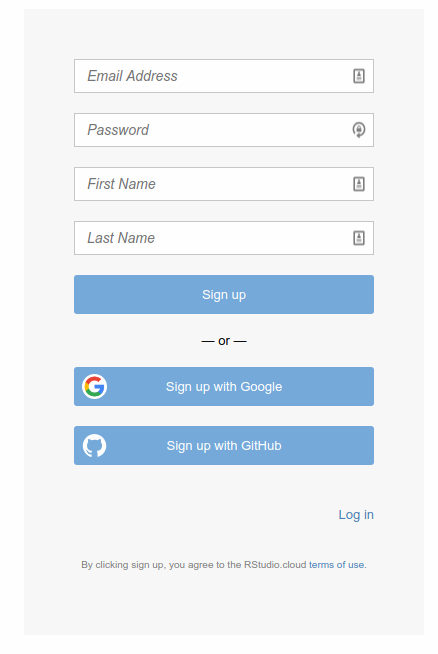
\includegraphics{Screenshot_2018-07-02_14-44-18.png}

If you're happy with using your Google account, click that button. You
will probably have to enter your Google password. (If you are doing this
on your own computer, you might not have to do that.) If you have a
GitHub account and you want to use \emph{that}, same principle. You can
also use an email address as your login to R Studio Cloud. (You can use
any e-mail address; I'm not checking.) Enter it in the top box, and
enter a password to use with R Studio Cloud in the second. (This does
not have to be, and indeed probably should not be, the same as your
email password.) Below that, enter your first and last name. This will
appear at the top right of the screen when you are logged in. Then click
Sign Up. After that, you will have to make a unique account name (which
\emph{you} actually never use, but which \texttt{rstudio.cloud} uses to
name your files). After that, you are automatically logged in.

\begin{enumerate}
\def\labelenumi{(\alph{enumi})}
\setcounter{enumi}{2}
\tightlist
\item
  Take a look around, and create a new Project. Give the new project any
  name you like.
\end{enumerate}

Solution

This is what you see now:

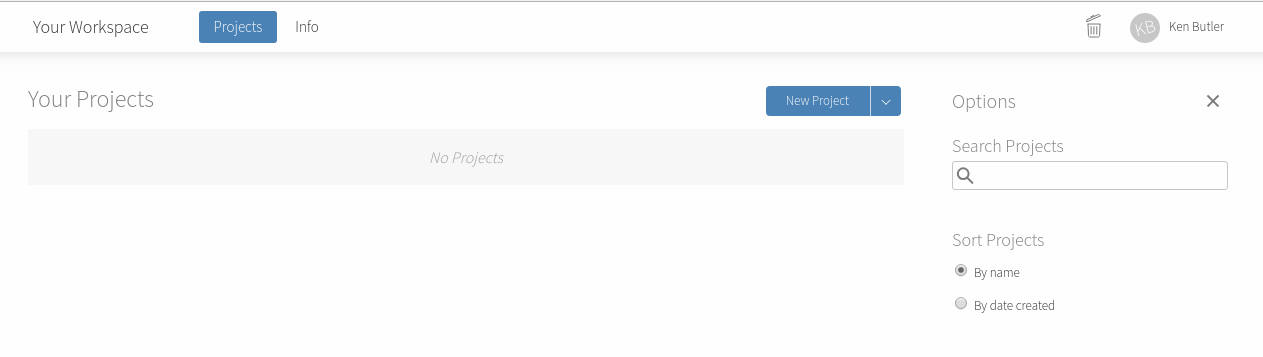
\includegraphics{Screenshot_2018-07-02_15-08-07.png}

Click on the blue New Project button to create a new Project. (A project
is a self-contained piece of work, like for example an assignment.) You
will see the words ``Loading Project'' and spinning circles for a few
moments. Then you see this:

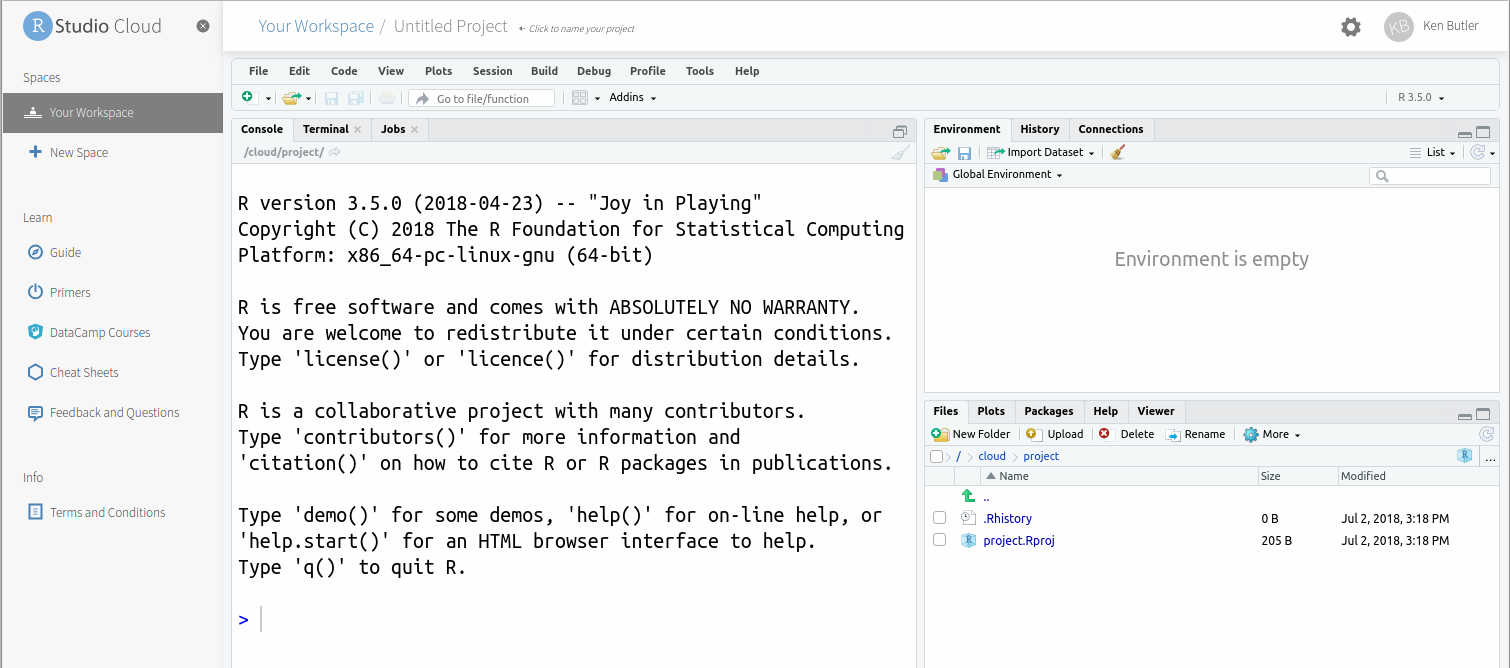
\includegraphics{Screenshot_2018-07-02_15-19-12.png}

To give your project a name, click at the top where it says Untitled
Project and type a name like Assignment 0 into the box.

\begin{enumerate}
\def\labelenumi{(\alph{enumi})}
\setcounter{enumi}{3}
\tightlist
\item
  Before we get to work, look for the blue \texttt{\textgreater{}} at
  the bottom left. Click next to it to get a flashing cursor, and then
  type what you see here (in blue):
\end{enumerate}

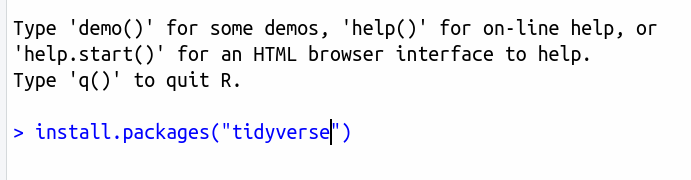
\includegraphics{Screenshot_2018-07-02_15-25-20.png}

Then press Enter.

Solution

This lets it install a bunch of things. It may take some time. If you
are watching it, look out for lines beginning with \texttt{g++}, which
are C++ code that needs to be compiled. This is the end of what I had.
Look out for the word DONE near the bottom:

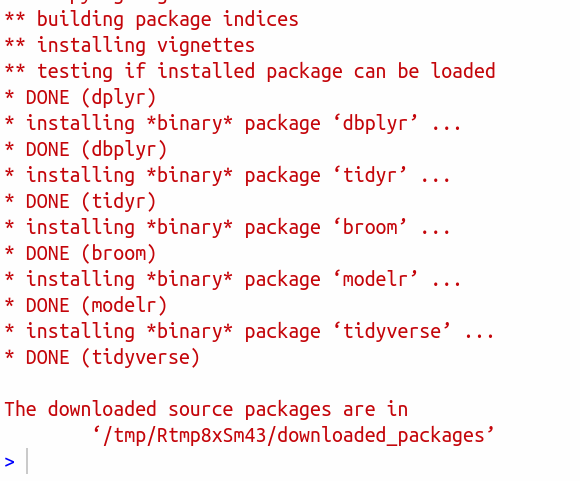
\includegraphics{Screenshot_2018-07-02_15-34-40.png}

\begin{enumerate}
\def\labelenumi{(\alph{enumi})}
\setcounter{enumi}{4}
\tightlist
\item
  Not for now, but for later: if you are on a lab computer, you should
  probably log out when you are done. To do that, find your name at the
  top right. Click on it, and two things should pop out to the right:
  Profile and Log Out. Select Log Out. You should be returned to one of
  the screens you began with, possibly the Welcome to R Studio Cloud
  one. To log back in, now or next time, look for Log In at the top
  right. Click it, to get this:
\end{enumerate}

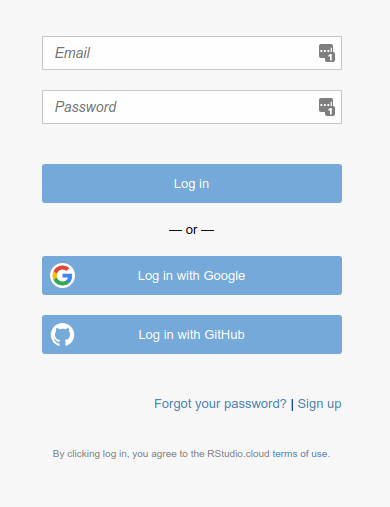
\includegraphics{Screenshot_2018-07-02_15-54-17.png}

and then you can log in with your email and password, or Google or
Github IDs, whichever you used. Now we can get down to some actual work.

\hypertarget{getting-started}{%
\section{Getting started}\label{getting-started}}

This question is to get you started using R.

\begin{enumerate}
\def\labelenumi{(\alph{enumi})}
\tightlist
\item
  Start R Studio Cloud, in some project. (If you started up a new
  project in the previous question and are still logged in, use that; if
  not, create a new project.)
\end{enumerate}

Solution

You ought to see something like this. I have a dark blue background
here, which you probably do not.

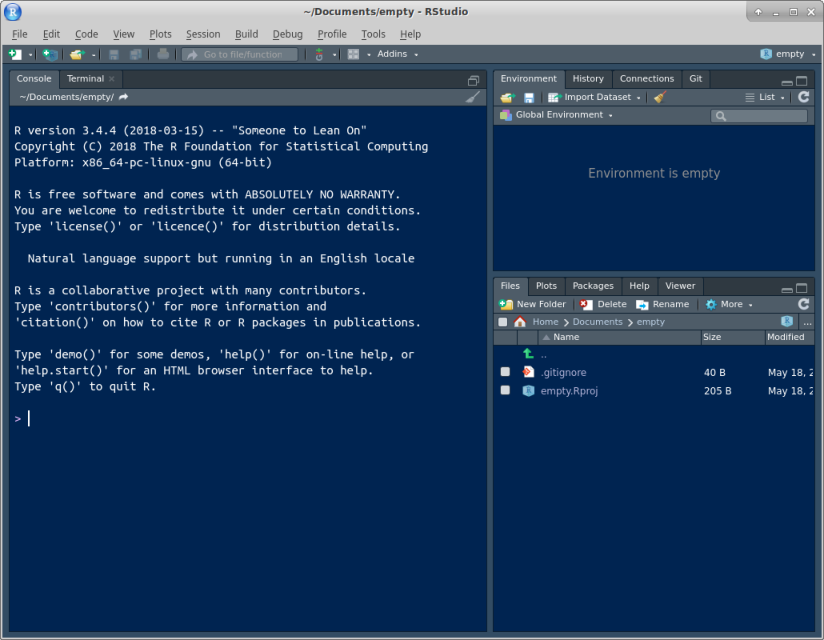
\includegraphics{empty.png}

It won't look exactly like that (for example, the background will
probably be white) but there should be one thing on the left half, and
at the top right it'll say ``Environment is empty''. Extra: if you want
to tweak things, select Tools (at the top of the screen) and from it
Global Options, then click Appearance. You can make the text bigger or
smaller via Editor Font Size, and choose a different colour scheme by
picking one of the Editor Themes (which previews on the right). My
favourite is Tomorrow Night Blue. Click Apply or OK when you have found
something you like. (I spend a lot of time in R Studio, and I like
having a dark background to be easier on my eyes.)

\begin{enumerate}
\def\labelenumi{(\alph{enumi})}
\setcounter{enumi}{1}
\tightlist
\item
  We're going to do some stuff in R here, just to get used to it. First,
  make an R Notebook by selecting File, New File and R Notebook.
\end{enumerate}

Solution

The first time, you'll be invited to ``install some packages'' to make
the Notebook thing work. Let it do that by clicking Yes. After that,
you'll have this:

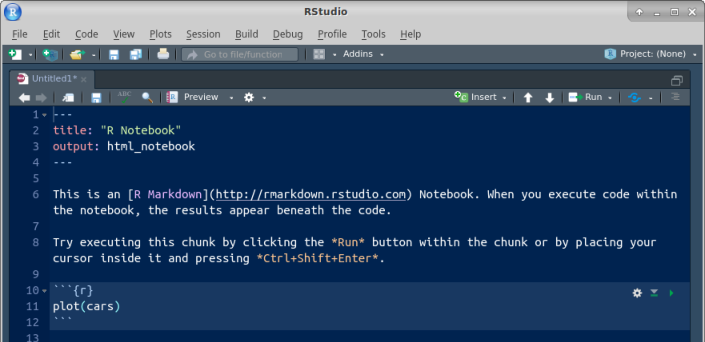
\includegraphics{rnote1.png}

Find the Insert and Run buttons along the top of the R Notebook window.
We'll be using them shortly. (The template notebook may or may not be
maximized; it doesn't matter either way. You might see all four panes or
as few as one. If you want to control that, select View at the top, then
Panes, then either Show All Panes or Zoom Source, as you prefer. In the
menus, you'll also see keyboard shortcuts for these, which you might
find worth learning.)

\begin{enumerate}
\def\labelenumi{(\alph{enumi})}
\setcounter{enumi}{2}
\tightlist
\item
  Change the title to something of your choosing. Then go down to line
  5, click on the Insert button and select R. You should see a ``code
  chunk'' appear at line 5, which we are going to use in a moment.
\end{enumerate}

Solution

Something like this:

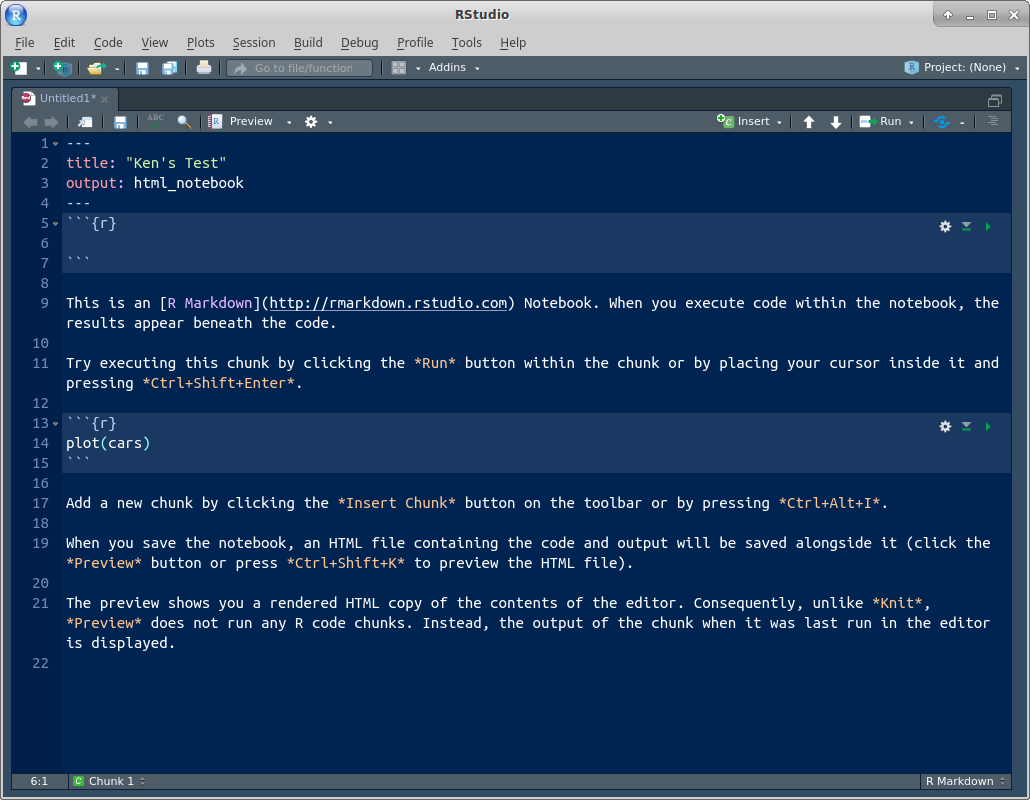
\includegraphics{chunk1.png}

\begin{enumerate}
\def\labelenumi{(\alph{enumi})}
\setcounter{enumi}{3}
\tightlist
\item
  Type the line of code shown below into the chunk in the R Notebook:
\end{enumerate}

\begin{verbatim}

mtcars
\end{verbatim}

Solution

What this will do: get hold of a built-in data set with information
about some different models of car, and display it.

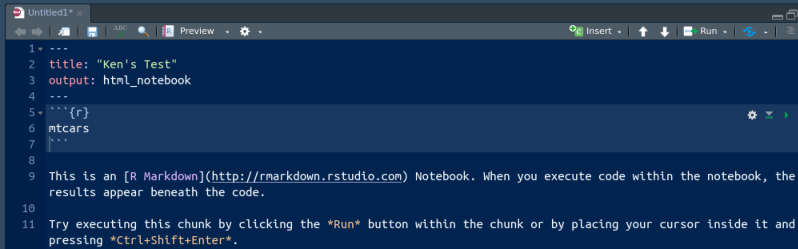
\includegraphics{chunk2.png}

In approximately five seconds, you'll be demonstrating that for
yourself.

\begin{enumerate}
\def\labelenumi{(\alph{enumi})}
\setcounter{enumi}{4}
\tightlist
\item
  Run this command. To do that, look at the top right of your code chunk
  block (shaded in a slightly different colour). You should see a gear
  symbol, a down arrow and a green ``play button''. Click the play
  button. This will run the code, and show the output below the code
  chunk.
\end{enumerate}

Solution

Here's what I get (yours will be the same).

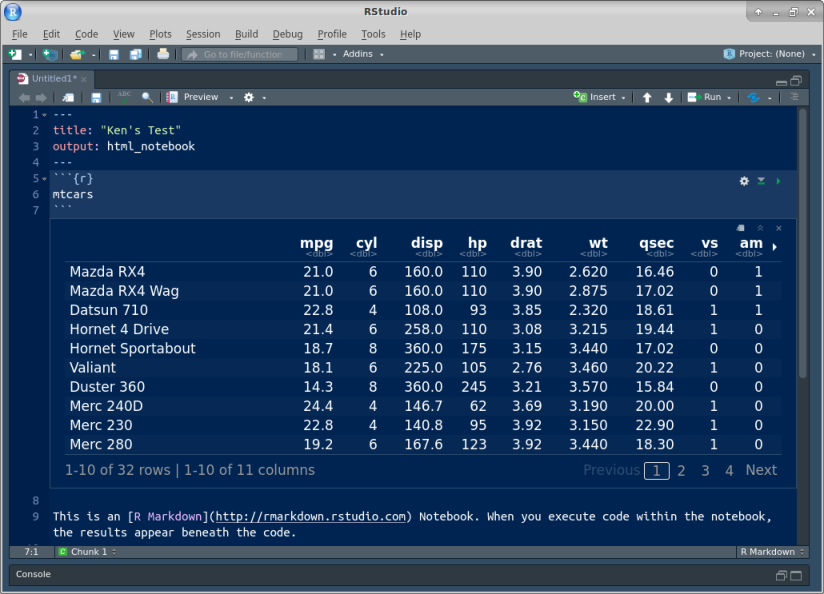
\includegraphics{chunk3.png}

This is a rectangular array of rows and columns, with individuals in
rows and variables in columns, known as a ``data frame''. When you
display a data frame in an R Notebook, you see 10 rows and as many
columns as will fit on the screen. At the bottom, it says how many rows
and columns there are altogether (here 32 rows and 11 columns), and
which ones are being displayed. You can see more rows by clicking on
Next, and if there are more columns, you'll see a little arrow next to
the rightmost column (as here next to \texttt{am}) that you can click on
to see more columns. Try it and see. Or if you want to go to a
particular collection of rows, click one of the numbers between Previous
and Next: 1 is rows 1--10, 2 is rows 11--20, and so on. The column on
the left without a header (containing the names of the cars) is called
``row names''. These have a funny kind of status, kind of a column and
kind of not a column; usually, if we need to use the names, we have to
put them in a column first. In future solutions, rather than showing you
a screenshot, expect me to show you something like this:

\begin{Shaded}
\begin{Highlighting}[]
\NormalTok{mtcars}
\end{Highlighting}
\end{Shaded}

\begin{verbatim}
## # A tibble: 32 x 11
##      mpg   cyl  disp    hp  drat    wt  qsec
##  * <dbl> <dbl> <dbl> <dbl> <dbl> <dbl> <dbl>
##  1  21       6  160    110  3.9   2.62  16.5
##  2  21       6  160    110  3.9   2.88  17.0
##  3  22.8     4  108     93  3.85  2.32  18.6
##  4  21.4     6  258    110  3.08  3.22  19.4
##  5  18.7     8  360    175  3.15  3.44  17.0
##  6  18.1     6  225    105  2.76  3.46  20.2
##  7  14.3     8  360    245  3.21  3.57  15.8
##  8  24.4     4  147.    62  3.69  3.19  20  
##  9  22.8     4  141.    95  3.92  3.15  22.9
## 10  19.2     6  168.   123  3.92  3.44  18.3
## # ... with 22 more rows, and 4 more
## #   variables: vs <dbl>, am <dbl>,
## #   gear <dbl>, carb <dbl>
\end{verbatim}

The top bit is the code, the bottom bit with the \texttt{\#\#} the
output. In this kind of display, you only see the first ten rows (by
default).

If you don't see the ``play button'', make sure that what you have
really is a code chunk. (I often accidentally delete one of the special
characters above or below the code chunk). If you can't figure it out,
delete this code chunk and make a new one. Sometimes R Studio gets
confused.

On the code chunk, the other symbols are the settings for this chunk
(you have the choice to display or not display the code or the output or
to not actually run the code). The second one, the down arrow, runs all
the chunks prior to this one (but not this one).

The output has its own little buttons. The first one pops the output out
into its own window; the second one shows or hides the output, and the
third one deletes the output (so that you have to run the chunk again to
get it back). Experiment. You can't do much damage here.

\begin{enumerate}
\def\labelenumi{(\alph{enumi})}
\setcounter{enumi}{5}
\tightlist
\item
  Something a little more interesting: \texttt{summary} obtains a
  summary of whatever you feed it (the five-number summary plus the mean
  for numerical variables). Obtain this for our data frame. To do this,
  create a new code chunk below the previous one, type
  \texttt{summary(mtcars)} into the code chunk, and run it.
\end{enumerate}

Solution

This is what you should see:

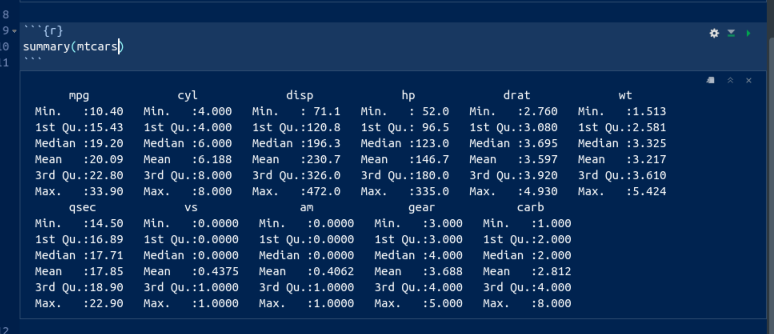
\includegraphics{chunk4.png}

or the other way:

\begin{Shaded}
\begin{Highlighting}[]
\KeywordTok{summary}\NormalTok{(mtcars)}
\end{Highlighting}
\end{Shaded}

\begin{verbatim}
##       mpg             cyl       
##  Min.   :10.40   Min.   :4.000  
##  1st Qu.:15.43   1st Qu.:4.000  
##  Median :19.20   Median :6.000  
##  Mean   :20.09   Mean   :6.188  
##  3rd Qu.:22.80   3rd Qu.:8.000  
##  Max.   :33.90   Max.   :8.000  
##       disp             hp       
##  Min.   : 71.1   Min.   : 52.0  
##  1st Qu.:120.8   1st Qu.: 96.5  
##  Median :196.3   Median :123.0  
##  Mean   :230.7   Mean   :146.7  
##  3rd Qu.:326.0   3rd Qu.:180.0  
##  Max.   :472.0   Max.   :335.0  
##       drat             wt       
##  Min.   :2.760   Min.   :1.513  
##  1st Qu.:3.080   1st Qu.:2.581  
##  Median :3.695   Median :3.325  
##  Mean   :3.597   Mean   :3.217  
##  3rd Qu.:3.920   3rd Qu.:3.610  
##  Max.   :4.930   Max.   :5.424  
##       qsec             vs        
##  Min.   :14.50   Min.   :0.0000  
##  1st Qu.:16.89   1st Qu.:0.0000  
##  Median :17.71   Median :0.0000  
##  Mean   :17.85   Mean   :0.4375  
##  3rd Qu.:18.90   3rd Qu.:1.0000  
##  Max.   :22.90   Max.   :1.0000  
##        am              gear      
##  Min.   :0.0000   Min.   :3.000  
##  1st Qu.:0.0000   1st Qu.:3.000  
##  Median :0.0000   Median :4.000  
##  Mean   :0.4062   Mean   :3.688  
##  3rd Qu.:1.0000   3rd Qu.:4.000  
##  Max.   :1.0000   Max.   :5.000  
##       carb      
##  Min.   :1.000  
##  1st Qu.:2.000  
##  Median :2.000  
##  Mean   :2.812  
##  3rd Qu.:4.000  
##  Max.   :8.000
\end{verbatim}

For the gas mileage column \texttt{mpg}, the mean is bigger than the
median, and the largest value is unusually large compared with the
others, suggesting a distribution that is skewed to the right.

There are 11 numeric (quantitative) variables, so we get the five-number
summary plus mean for each one. Categorical variables, if we had any
here, would be displayed a different way.

(In case you are wondering, the way without screenshots is obtained by
\emph{my} writing a notebook with code chunks and running them, so this
output genuinely \emph{is} obtained by running the code you see.)

\begin{enumerate}
\def\labelenumi{(\alph{enumi})}
\setcounter{enumi}{6}
\tightlist
\item
  Let's make a boxplot of the gas mileage data. This is a ``poor man's
  boxplot''; we'll see a nicer-looking way later. To do it this way,
  make another new code chunk, enter the code
  \texttt{boxplot(mtcars\$mpg)} into it, and run the chunk.
\end{enumerate}

Solution

This is what you should see:

\begin{Shaded}
\begin{Highlighting}[]
\KeywordTok{boxplot}\NormalTok{(mtcars}\OperatorTok{$}\NormalTok{mpg)}
\end{Highlighting}
\end{Shaded}

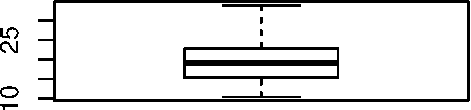
\includegraphics{01-getting-used_files/figure-latex/unnamed-chunk-8-1}

The long upper whisker supports our guess from before that the
distribution is right-skewed.

\begin{enumerate}
\def\labelenumi{(\alph{enumi})}
\setcounter{enumi}{7}
\tightlist
\item
  Some aesthetics to finish with: delete the template notebook (all the
  stuff you didn't type below your code chunks and output). Then add
  some narrative text above and below your code chunks. Above the code
  chunk is where you say what you are going to do (and maybe why you are
  doing it), and below is where you say what you conclude from the
  output you just obtained.
\end{enumerate}

Solution

My complete R Notebook is at
\url{http://www.utsc.utoronto.ca/~butler/c32/a0-notebook-1.Rmd}. Take a
look at it. I added one extra thing: my variable names have
``backticks'' around them. You'll see the effect of this in a moment.
Backtick is on the key to the left of 1 and below Esc on your keyboard,
along with a ``squiggle'' symbol that we'll be using later in the
course.

\begin{enumerate}
\def\labelenumi{(\roman{enumi})}
\tightlist
\item
  Save your notebook (the usual way with File and Save). This saves it
  \emph{on the R Studio Cloud servers} (and not on your computer). This
  means that when you come back to R Studio Cloud later, even from
  another device, this notebook will still be available to you. Now
  click Preview. This produces a pretty HTML version of your notebook.
\end{enumerate}

Solution

Note that the HTML document only contains output from the chunks you've
run in the notebook, so it's up to you to run them there first.\\
My HTML document is at
\url{http://www.utsc.utoronto.ca/~butler/c32/a0-notebook-1.nb.html}.
Here's where you see the effect of the backticks: all the variable names
are in \texttt{typewriter\ font} so that you can see they are variable
names and not something else. If you want to try this notebook out
yourself, you have a couple of options: (i) make a new R Notebook on R
Studio Cloud and copy-paste the contents of my file (it's just text), or
(ii) download my R Notebook onto your computer, and then upload it to R
Studio Cloud. Look in the Files pane bottom right, and next to New
Folder you should see Upload. Upload the file from wherever it got saved
to when you downloaded it. Extra: if you're feeling ambitious, click the
arrow to the right of Preview and select Knit to Word. The button
changes to Knit with a ball of wool beside it. Now, when you ``knit''
the notebook, you get a Word document directly --- look for it in the
Files pane. If you want to, you can hand this kind of thing in (on later
assignments), but you'll have to do a little work first: first, find it
in your Files list, then click the checkbox to the left of it, then
click More (with the gear, on the same line as New Folder and Upload),
then select Export (and click Download). This will put a copy in your
downloads folder on your computer, and you can open it from there. If
you're feeling extra-ambitious, you can try Knit to PDF. This produces
something that looks as if it was written in LaTeX, but actually wasn't.
To make this work, if you have a \texttt{library(tidyverse)} line
somewhere, as you probably will, find the code chunk it's in, and make
it look like this:

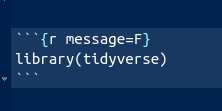
\includegraphics{Screenshot_2018-10-10_17-24-47.png}

Then it will work. Extra extra: if you like the keyboard better than the
mouse, R Studio has a lot of keyboard shortcuts. Two that are useful
now: control-alt-i inserts a code chunk where the cursor is, and
control-shift-enter runs the code chunk that the cursor is in, if it is
in one. (Mac users, ``command'' instead of ``control'' in both cases.) I
use these two a lot.

\begin{enumerate}
\def\labelenumi{(\alph{enumi})}
\setcounter{enumi}{9}
\tightlist
\item
  Optional extra: practice handing in your previewed R notebook, as if
  it were an assignment that was worth something. (It is good to get the
  practice in a low-stakes situation, so that you'll know what to do
  next week.)
\end{enumerate}

Solution

There are two steps: download the HTML file onto your computer, and then
handing it in on Quercus. To download: find the HTML file that you want
to download in the Files pane bottom right. There should be two files
starting with the same thing, eg. \texttt{test1.Rmd}, which is the
notebook you wrote, and \texttt{test1.nb.html}, which is the previewed
version of it, and is the one you want to download. (The \texttt{test1}
part is the name \emph{you} chose when you saved it.) Click the checkbox
to the left of the HTML file. Now click on More above the bottom-right
pane. This pops up a menu from which you choose Export. This will pop up
another window called Export Files, where you put the name that the file
will have on your computer. (I usually leave the name the same.) Click
Download. The file will go to your Downloads folder, or wherever things
you download off the web go. Now, to hand it in. Open up Quercus at
\texttt{q.utoronto.ca}, log in and navigate to this course. Click
Assignments. Click (the title of) Assignment 0. There is a big blue
Submit Assignment button top right. Click it. You'll get a File Upload
at the bottom of the screen. Click Choose File and find the HTML file
that you downloaded. Click Open (or equivalent on your system). The name
of the file should appear next to Choose File. Click Submit Assignment.
You'll see Submitted at the top right. If you want to try this again,
you can Re-submit Assignment as many times as you like. (For the real
thing, you can use this if you realize you made a mistake in something
you submitted. The graders' instructions, for the real thing, are to
grade the \emph{last} file submitted, so in that case you need to make
sure that the last thing submitted includes \emph{everything} that you
want graded. Here, though, it doesn't matter.)

\begin{enumerate}
\def\labelenumi{(\alph{enumi})}
\setcounter{enumi}{10}
\tightlist
\item
  Optional extra. Something more ambitious: make a scatterplot of gas
  mileage \texttt{mpg}, on the \(y\) axis, against horsepower,
  \texttt{hp}, on the \(x\)-axis.
\end{enumerate}

Solution

That goes like this. I'll explain the steps below.

\begin{Shaded}
\begin{Highlighting}[]
\KeywordTok{library}\NormalTok{(tidyverse)}
\KeywordTok{ggplot}\NormalTok{(mtcars, }\KeywordTok{aes}\NormalTok{(}\DataTypeTok{x =}\NormalTok{ hp, }\DataTypeTok{y =}\NormalTok{ mpg)) }\OperatorTok{+}\StringTok{ }\KeywordTok{geom_point}\NormalTok{()}
\end{Highlighting}
\end{Shaded}

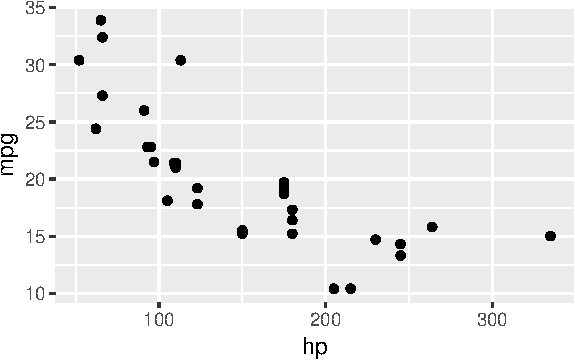
\includegraphics{01-getting-used_files/figure-latex/unnamed-chunk-9-1}
\$ \%\$ \%\$

This shows a somewhat downward trend, which is what you'd expect, since
a larger \texttt{hp} value means a more powerful engine, which will
probably consume more gas and get \emph{fewer} miles per gallon. As for
the code: to make a \texttt{ggplot} plot, as we will shortly see in
class, you first need a \texttt{ggplot} statement that says what to
plot. The first thing in a \texttt{ggplot} is a data frame
(\texttt{mtcars} here), and then the \texttt{aes} says that the plot
will have \texttt{hp} on the \(x\)-axis and \texttt{mpg} on the
\(y\)-axis, taken from the data frame that you specified. That's all of
the what-to-plot. The last thing is how to plot it;
\texttt{geom\_point()} says to plot the data values as points.

You might like to add a regression line to the plot. That is a matter of
adding this to the end of the plotting command:

\begin{Shaded}
\begin{Highlighting}[]
\KeywordTok{ggplot}\NormalTok{(mtcars, }\KeywordTok{aes}\NormalTok{(}\DataTypeTok{x =}\NormalTok{ hp, }\DataTypeTok{y =}\NormalTok{ mpg)) }\OperatorTok{+}\StringTok{ }\KeywordTok{geom_point}\NormalTok{() }\OperatorTok{+}\StringTok{ }
\StringTok{    }\KeywordTok{geom_smooth}\NormalTok{(}\DataTypeTok{method =} \StringTok{"lm"}\NormalTok{)}
\end{Highlighting}
\end{Shaded}

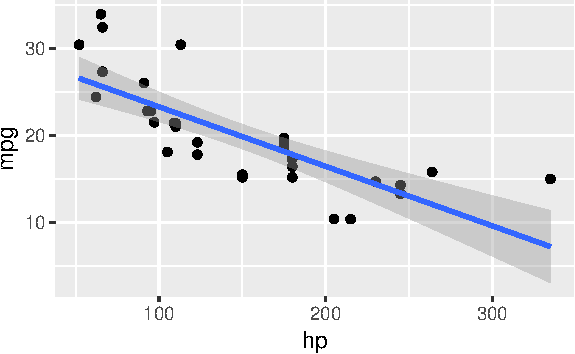
\includegraphics{01-getting-used_files/figure-latex/unnamed-chunk-10-1}

The line definitely goes downhill. Decide for yourself how well you
think a line fits these data.

\hypertarget{reading-data-from-a-file}{%
\section{Reading data from a file}\label{reading-data-from-a-file}}

In this question, we read a file from the web and do some descriptive
statistics and a graph. This is very like what you will be doing on
future assignments, so it's good to practice it now.

Take a look at the data file at
\url{https://www.utsc.utoronto.ca/~butler/c32/jumping.txt}. These are
measurements on 30 rats that were randomly made to do different amounts
of jumping by group (we'll see the details later in the course). The
control group did no jumping, and the other groups did ``low jumping''
and ``high jumping''. The first column says which jumping group each rat
was in, and the second is the rat's bone density (the experimenters'
supposition was that more jumping should go with higher bone density).

\begin{enumerate}
\def\labelenumi{(\alph{enumi})}
\tightlist
\item
  What are the two columns of data separated by? (The fancy word is
  ``delimited'').
\end{enumerate}

Solution

Exactly one space. This is true all the way down, as you can check.

\begin{enumerate}
\def\labelenumi{(\alph{enumi})}
\setcounter{enumi}{1}
\tightlist
\item
  Make a new R Notebook. Leave the first four lines, but get rid of the
  rest of the template document. Start with a code chunk containing
  \texttt{library(tidyverse)}. Run it.
\end{enumerate}

Solution

You will get either the same message as before or nothing. (I got
nothing because I had already loaded the \texttt{tidyverse} in this
session.)

\begin{enumerate}
\def\labelenumi{(\alph{enumi})}
\setcounter{enumi}{2}
\tightlist
\item
  Put the URL of the data file in a variable called \texttt{my\_url}.
  Then use \texttt{read\_delim} to read in the file. (See solutions for
  how.) \texttt{read\_delim} reads data files where the data values are
  always separated by the same single character, here a space. Save the
  data frame in a variable \texttt{rats}.
\end{enumerate}

Solution

Like this:

\begin{Shaded}
\begin{Highlighting}[]
\NormalTok{my_url =}\StringTok{ "https://www.utsc.utoronto.ca/~butler/c32/jumping.txt"}
\NormalTok{rats =}\StringTok{ }\KeywordTok{read_delim}\NormalTok{(my_url, }\StringTok{" "}\NormalTok{)}
\end{Highlighting}
\end{Shaded}

\begin{verbatim}
## Parsed with column specification:
## cols(
##   group = col_character(),
##   density = col_integer()
## )
\end{verbatim}

The second thing in \texttt{read\_delim} is the thing that separates the
data values. Often when you use \texttt{read\_delim} it'll be a space.

\begin{enumerate}
\def\labelenumi{(\alph{enumi})}
\setcounter{enumi}{3}
\tightlist
\item
  Take a look at your data frame, by making a new code chunk and putting
  the data frame's name in it (as we did with \texttt{mtcars}).
\end{enumerate}

Solution

\begin{Shaded}
\begin{Highlighting}[]
\NormalTok{rats}
\end{Highlighting}
\end{Shaded}

\begin{verbatim}
## # A tibble: 30 x 2
##    group   density
##    <chr>     <int>
##  1 Control     611
##  2 Control     621
##  3 Control     614
##  4 Control     593
##  5 Control     593
##  6 Control     653
##  7 Control     600
##  8 Control     554
##  9 Control     603
## 10 Control     569
## # ... with 20 more rows
\end{verbatim}

There are 30 rows and two columns, as there should be.

\begin{enumerate}
\def\labelenumi{(\alph{enumi})}
\setcounter{enumi}{4}
\tightlist
\item
  Find the mean bone density for rats that did each amount of jumping.
\end{enumerate}

Solution

This is something you'll see a lot: \texttt{group\_by} followed by
\texttt{summarize}. Reminder: to get that funny thing with the percent
signs (called the ``pipe symbol''), type control-shift-M (or equivalent
on a Mac):

\begin{Shaded}
\begin{Highlighting}[]
\NormalTok{rats }\OperatorTok\StringTok{ }\KeywordTok{group_by}\NormalTok{(group) }\OperatorTok\StringTok{ }\KeywordTok{summarize}\NormalTok{(}\DataTypeTok{m =} \KeywordTok{mean}\NormalTok{(density))}
\end{Highlighting}
\end{Shaded}

\begin{verbatim}
## # A tibble: 3 x 2
##   group        m
##   <chr>    <dbl>
## 1 Control   601.
## 2 Highjump  639.
## 3 Lowjump   612.
\end{verbatim}

The mean bone density is clearly highest for the high jumping group, and
not much different between the low-jumping and control groups.

\begin{enumerate}
\def\labelenumi{(\alph{enumi})}
\setcounter{enumi}{5}
\tightlist
\item
  Make a boxplot of bone density for each jumping group.
\end{enumerate}

Solution

On a boxplot, the groups go across and the values go up and down, so the
right syntax is this:

\begin{Shaded}
\begin{Highlighting}[]
\KeywordTok{ggplot}\NormalTok{(rats, }\KeywordTok{aes}\NormalTok{(}\DataTypeTok{x =}\NormalTok{ group, }\DataTypeTok{y =}\NormalTok{ density)) }\OperatorTok{+}\StringTok{ }\KeywordTok{geom_boxplot}\NormalTok{()}
\end{Highlighting}
\end{Shaded}

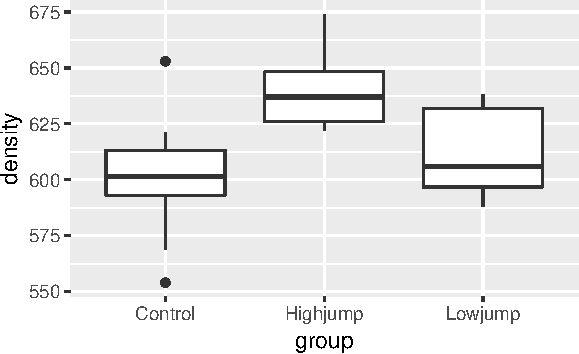
\includegraphics{01-getting-used_files/figure-latex/unnamed-chunk-14-1}

Given the amount of variability, the control and low-jump groups are
very similar (with the control group having a couple of outliers), but
the high-jump group seems to have a consistently higher bone density
than the others.

This is more or less in line with what the experimenters were guessing,
but it seems that it has to be high jumping to make a difference.

You might recognize that this is the kind of data where we would use
analysis of variance, which we will do later on in the course: we are
comparing several (here three) groups.

\hypertarget{reading-in-data-and-drawing-some-graphs}{%
\chapter{Reading in data and drawing some
graphs}\label{reading-in-data-and-drawing-some-graphs}}

\hypertarget{orange-juice}{%
\section{Orange juice}\label{orange-juice}}

The quality of orange juice produced by a manufacturer (identity
unknown) is constantly being monitored. The manufacturer has developed a
``sweetness index'' for its orange juice, for which a higher value means
sweeter juice. Is the sweetness index related to a chemical measure such
as the amount of water-soluble pectin (parts per million) in the orange
juice? Data were obtained from 24 production runs, and the sweetness and
pectin content were measured for each run. The data are in
\href{http://www.utsc.utoronto.ca/~butler/c32/ojuice.txt}{link}. Open
that link up now. You can click on that link just above to open the
file.

\begin{enumerate}
\def\labelenumi{(\alph{enumi})}
\tightlist
\item
  The data values are separated by a space. Use the appropriate
  Tidyverse function to read the data directly from the course website
  into a ``tibble''.
\end{enumerate}

Solution

Start with this (almost always):

\begin{Shaded}
\begin{Highlighting}[]
\KeywordTok{library}\NormalTok{(tidyverse)}
\end{Highlighting}
\end{Shaded}

\begin{verbatim}
## -- Attaching packages ---- tidyverse 1.2.1 --
\end{verbatim}

\begin{verbatim}
## v ggplot2 3.0.0     v purrr   0.2.5
## v tibble  1.4.2     v dplyr   0.7.6
## v tidyr   0.8.1     v stringr 1.3.1
## v readr   1.1.1     v forcats 0.3.0
\end{verbatim}

\begin{verbatim}
## -- Conflicts ------- tidyverse_conflicts() --
## x dplyr::filter() masks stats::filter()
## x dplyr::lag()    masks stats::lag()
\end{verbatim}

The appropriate function, the data values being separated by a space,
will be \texttt{read\_delim}. Put the URL as the first thing in
\texttt{read\_delim}, or (better) define it into a variable first:
\marginnote{I say *better* because otherwise the read line gets rather long. This way you read it as *the URL is some long thing that I don't care about especially, and I what I need to do is to read the data from that URL, separated by spaces.*}

\begin{Shaded}
\begin{Highlighting}[]
\NormalTok{url =}\StringTok{ "http://www.utsc.utoronto.ca/~butler/c32/ojuice.txt"}
\NormalTok{juice =}\StringTok{ }\KeywordTok{read_delim}\NormalTok{(url, }\StringTok{" "}\NormalTok{)}
\end{Highlighting}
\end{Shaded}

\begin{verbatim}
## Parsed with column specification:
## cols(
##   run = col_integer(),
##   sweetness = col_double(),
##   pectin = col_integer()
## )
\end{verbatim}

\texttt{read\_delim} (or \texttt{read\_csv} or any of the others) tell
you what variables were read in, and also tell you about any ``parsing
errors'' where it couldn't work out what was what. Here, we have three
variables, which is entirely consistent with the three columns of data
values in the file.

\texttt{read\_delim} can handle data values separated by \emph{any}
character, not just spaces, but the separating character, known as a
``delimiter'', does \emph{not} have a default, so you have to say what
it is, every time.

\begin{enumerate}
\def\labelenumi{(\alph{enumi})}
\setcounter{enumi}{1}
\tightlist
\item
  Take a look at what got read in. Do you have data for all 24 runs?
\end{enumerate}

Solution

Type the name of the data frame in a code chunk (a new one, or add it to
the end of the previous one). Because this is actually a ``tibble'',
which is what \texttt{read\_delim} reads in, you'll only actually see
the first 10 lines, but it will tell you how many lines there are
altogether, and you can click on the appropriate thing to see the rest
of it.

\begin{Shaded}
\begin{Highlighting}[]
\NormalTok{juice}
\end{Highlighting}
\end{Shaded}

\begin{verbatim}
## # A tibble: 24 x 3
##      run sweetness pectin
##    <int>     <dbl>  <int>
##  1     1       5.2    220
##  2     2       5.5    227
##  3     3       6      259
##  4     4       5.9    210
##  5     5       5.8    224
##  6     6       6      215
##  7     7       5.8    231
##  8     8       5.6    268
##  9     9       5.6    239
## 10    10       5.9    212
## # ... with 14 more rows
\end{verbatim}

I appear to have all the data. If you want further convincing, click
Next a couple of times (on yours) to be sure that the runs go down to
number 24.

\begin{enumerate}
\def\labelenumi{(\alph{enumi})}
\setcounter{enumi}{2}
\tightlist
\item
  In your data frame, where did the column (variable) names come from?
  How did R know where to get them from?
\end{enumerate}

Solution

They came from the top line of the data file, so we didn't have to
specify them. This is the default behaviour of all the \texttt{read\_}
functions, so we don't have to ask for it specially. In fact, if the top
line of your data file is \emph{not} variable names, \emph{that's} when
you have to say something special. The \texttt{read\_} functions have an
option \texttt{col\_names} which can either be \texttt{TRUE} (the
default), which means ``read them in from the top line'', \texttt{FALSE}
(``they are not there, so make some up'') or a list of column names to
use. You might use the last alternative when the column names that are
in the file are \emph{not} the ones you want to use; in that case, you
would also say \texttt{skip=1} to skip the first line. For example, with
file \texttt{a.txt} thus: \texttt{timinput\{}.txt\}\\
you could read the same data but call the columns \texttt{x} and
\texttt{y} thus:

\begin{Shaded}
\begin{Highlighting}[]
\KeywordTok{read_delim}\NormalTok{(}\StringTok{"a.txt"}\NormalTok{, }\StringTok{" "}\NormalTok{, }\DataTypeTok{col_names =} \KeywordTok{c}\NormalTok{(}\StringTok{"x"}\NormalTok{, }\StringTok{"y"}\NormalTok{), }
    \DataTypeTok{skip =} \DecValTok{1}\NormalTok{)}
\end{Highlighting}
\end{Shaded}

\begin{verbatim}
## Parsed with column specification:
## cols(
##   x = col_integer(),
##   y = col_integer()
## )
\end{verbatim}

\begin{verbatim}
## # A tibble: 3 x 2
##       x     y
##   <int> <int>
## 1     1     2
## 2     3     4
## 3     5     6
\end{verbatim}

\begin{enumerate}
\def\labelenumi{(\alph{enumi})}
\setcounter{enumi}{3}
\tightlist
\item
  The juice manufacturer was interested in whether there was a
  relationship between sweetness and pectin. To assess this, draw a
  scatterplot. Does it look as if there is any kind of a relationship?
  (I think \texttt{sweetness} is the outcome variable and
  \texttt{pectin} is explanatory, so draw your scatterplot
  appropriately.)
\end{enumerate}

Solution

This requires a \texttt{ggplot} plot. You can go back and look at the
lecture notes to figure out how to make a scatterplot: the ``what to
plot'' is the \(x\)-axis and \(y\)-axis variables, with the response on
the \(y\)-axis (starting with a data frame to get the variables from),
and the ``how to plot'' is \texttt{geom\_point} to plot the points:

\begin{Shaded}
\begin{Highlighting}[]
\KeywordTok{ggplot}\NormalTok{(juice, }\KeywordTok{aes}\NormalTok{(}\DataTypeTok{x =}\NormalTok{ pectin, }\DataTypeTok{y =}\NormalTok{ sweetness)) }\OperatorTok{+}\StringTok{ }
\StringTok{    }\KeywordTok{geom_point}\NormalTok{()}
\end{Highlighting}
\end{Shaded}

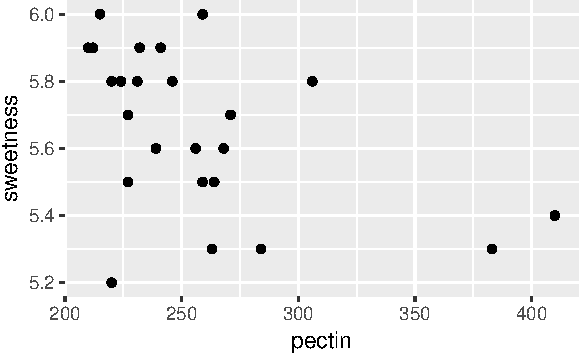
\includegraphics{02-reading-in_files/figure-latex/unnamed-chunk-8-1}

It looks to me as if there is a negative relationship: as pectin goes
up, sweetness tends to go \emph{down}. The trend appears to go top left
to bottom right.

Having said that, I'm wondering how much of the apparent trend is caused
by those two observations bottom right with pectin over 350. If you take
those away, the trend seems to me to be a lot less convincing. As an
extra, you could add a smooth trend to the plot:

\begin{Shaded}
\begin{Highlighting}[]
\KeywordTok{ggplot}\NormalTok{(juice, }\KeywordTok{aes}\NormalTok{(}\DataTypeTok{x =}\NormalTok{ pectin, }\DataTypeTok{y =}\NormalTok{ sweetness)) }\OperatorTok{+}\StringTok{ }
\StringTok{    }\KeywordTok{geom_point}\NormalTok{() }\OperatorTok{+}\StringTok{ }\KeywordTok{geom_smooth}\NormalTok{()}
\end{Highlighting}
\end{Shaded}

\begin{verbatim}
## `geom_smooth()` using method = 'loess' and formula 'y ~ x'
\end{verbatim}

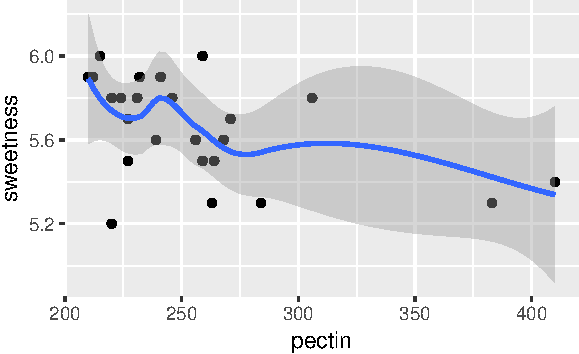
\includegraphics{02-reading-in_files/figure-latex/unnamed-chunk-9-1}

The smooth trend is kind of downhill, but not very convincing.

\hypertarget{making-soap}{%
\section{Making soap}\label{making-soap}}

A company operates two production lines in a factory for making soap
bars. The production lines are labelled A and B. A production line that
moves faster may produce more soap, but may possibly also produce more
``scrap'' (that is, bits of soap that can no longer be made into soap
bars and will have to be thrown away).

The data are in
\href{http://www.utsc.utoronto.ca/~butler/c32/soap.txt}{link}.

\begin{enumerate}
\def\labelenumi{(\alph{enumi})}
\tightlist
\item
  Read the data into R. Display the data. There should be 27 rows. Are
  there?
\end{enumerate}

Solution

Read directly from the URL, most easily:

\begin{Shaded}
\begin{Highlighting}[]
\NormalTok{url =}\StringTok{ "http://www.utsc.utoronto.ca/~butler/c32/soap.txt"}
\NormalTok{soap =}\StringTok{ }\KeywordTok{read_delim}\NormalTok{(url, }\StringTok{" "}\NormalTok{)}
\end{Highlighting}
\end{Shaded}

\begin{verbatim}
## Parsed with column specification:
## cols(
##   case = col_integer(),
##   scrap = col_integer(),
##   speed = col_integer(),
##   line = col_character()
## )
\end{verbatim}

\begin{Shaded}
\begin{Highlighting}[]
\NormalTok{soap}
\end{Highlighting}
\end{Shaded}

\begin{verbatim}
## # A tibble: 27 x 4
##     case scrap speed line 
##    <int> <int> <int> <chr>
##  1     1   218   100 a    
##  2     2   248   125 a    
##  3     3   360   220 a    
##  4     4   351   205 a    
##  5     5   470   300 a    
##  6     6   394   255 a    
##  7     7   332   225 a    
##  8     8   321   175 a    
##  9     9   410   270 a    
## 10    10   260   170 a    
## # ... with 17 more rows
\end{verbatim}

27 rows. \texttt{line}, which is either \texttt{a} or \texttt{b}, was
correctly deduced to be text.

\begin{enumerate}
\def\labelenumi{(\alph{enumi})}
\setcounter{enumi}{1}
\tightlist
\item
  Obtain a histogram of the \texttt{scrap} values, using 10 bins for
  your histogram.
\end{enumerate}

Solution

\begin{Shaded}
\begin{Highlighting}[]
\KeywordTok{ggplot}\NormalTok{(soap, }\KeywordTok{aes}\NormalTok{(}\DataTypeTok{x =}\NormalTok{ scrap)) }\OperatorTok{+}\StringTok{ }\KeywordTok{geom_histogram}\NormalTok{(}\DataTypeTok{bins =} \DecValTok{10}\NormalTok{)}
\end{Highlighting}
\end{Shaded}

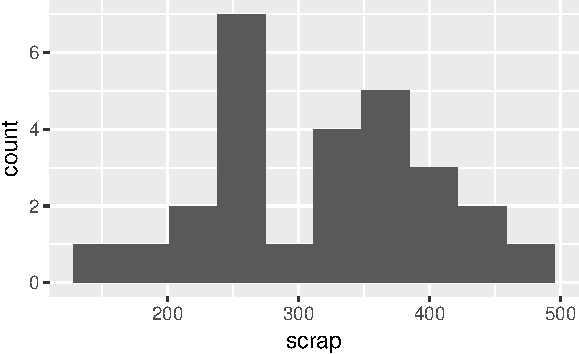
\includegraphics{02-reading-in_files/figure-latex/unnamed-chunk-11-1}

\begin{enumerate}
\def\labelenumi{(\alph{enumi})}
\setcounter{enumi}{2}
\tightlist
\item
  Comment briefly on the shape of the histogram. Is it approximately
  symmetric, skewed to the left, skewed to the right or something else?
  (By ``comment briefly'' I mean ``say in a few words why you gave the
  answer you did.'')
\end{enumerate}

Solution

I would call this ``bimodal''. There are two peaks to the histogram, one
around 250 and one around 370, with a very small frequency in between
(the bar around 300). Apart from the bimodality, there is no particular
evidence for a long tail on either end, so I don't think you could
otherwise call it anything other than symmetric. Having said that (this
is going beyond the question), the way a histogram looks can depend on
the bins you choose to draw it with. This is 8 bins rather than 10:

\begin{Shaded}
\begin{Highlighting}[]
\KeywordTok{ggplot}\NormalTok{(soap, }\KeywordTok{aes}\NormalTok{(}\DataTypeTok{x =}\NormalTok{ scrap)) }\OperatorTok{+}\StringTok{ }\KeywordTok{geom_histogram}\NormalTok{(}\DataTypeTok{bins =} \DecValTok{8}\NormalTok{)}
\end{Highlighting}
\end{Shaded}

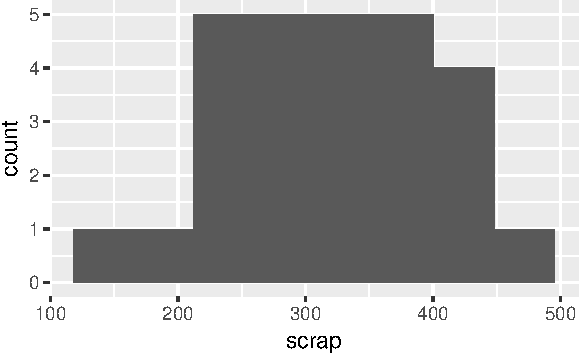
\includegraphics{02-reading-in_files/figure-latex/unnamed-chunk-12-1}

The middle low-frequency bin has gone, and this one just looks
symmetric, with a kind of ``flat top''.

\begin{enumerate}
\def\labelenumi{(\alph{enumi})}
\setcounter{enumi}{3}
\tightlist
\item
  Make side-by-side boxplots of scrap values for each production line.
\end{enumerate}

Solution

\begin{Shaded}
\begin{Highlighting}[]
\KeywordTok{ggplot}\NormalTok{(soap, }\KeywordTok{aes}\NormalTok{(}\DataTypeTok{x =}\NormalTok{ line, }\DataTypeTok{y =}\NormalTok{ scrap)) }\OperatorTok{+}\StringTok{ }\KeywordTok{geom_boxplot}\NormalTok{()}
\end{Highlighting}
\end{Shaded}

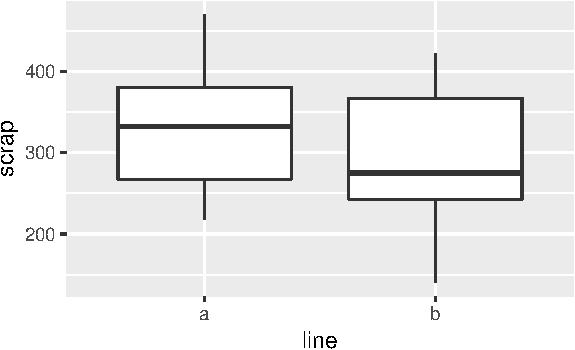
\includegraphics{02-reading-in_files/figure-latex/unnamed-chunk-13-1}

One categorical, one quantitative variable, so boxplots make sense.

\begin{enumerate}
\def\labelenumi{(\alph{enumi})}
\setcounter{enumi}{4}
\tightlist
\item
  Do you think your boxplot says that there are differences in the
  amount of scrap produced by the two production lines, or not? Explain
  briefly.
\end{enumerate}

Solution

I would say that there \emph{is} a difference between the two production
lines, with line A producing an average (median) of about 330 and line B
producing a median of about 275. But you could also make the case that,
although the medians are rather different, there is a lot of variability
and hence a lot of overlap between the two boxplots, and therefore that
there is not a ``substantial'' difference. I would say that either of
those answers are good \emph{if you
back them up with proper reasons}. This is going to be a common theme in
this course: I am going to ask you to make a decision and support it,
where the reasons you provide are often more important than the decision
you make. You might be wondering whether the medians, or means, since
there is no serious skewness here and definitely no outliers, are
``significantly different''. This is inference, which we will come to
later, but a preview looks like this:

\begin{Shaded}
\begin{Highlighting}[]
\KeywordTok{t.test}\NormalTok{(scrap }\OperatorTok{~}\StringTok{ }\NormalTok{line, }\DataTypeTok{data =}\NormalTok{ soap)}
\end{Highlighting}
\end{Shaded}

\begin{verbatim}
## 
##  Welch Two Sample t-test
## 
## data:  scrap by line
## t = 1.2493, df = 21.087, p-value =
## 0.2253
## alternative hypothesis: true difference in means is not equal to 0
## 95 percent confidence interval:
##  -26.97888 108.21222
## sample estimates:
## mean in group a mean in group b 
##        333.5333        292.9167
\end{verbatim}

They are not: the P-value of 0.22 is not anywhere near as small as 0.05,
so we can't reject the null hypothesis that the two lines have equal
mean amount of scrap.

Rusty on this stuff? Don't worry; we're going to come back to it later
in the course.

I was also wondering about something else: that bimodal histogram. Could
that be explained by the scrap values being two different production
lines being mixed together? One way to understand that is to have two
separate histograms, one for each line, side by side, which is what
facetting does. There is an extra wrinkle here that I explain
afterwards:

\begin{Shaded}
\begin{Highlighting}[]
\KeywordTok{ggplot}\NormalTok{(soap, }\KeywordTok{aes}\NormalTok{(}\DataTypeTok{x =}\NormalTok{ scrap)) }\OperatorTok{+}\StringTok{ }\KeywordTok{geom_histogram}\NormalTok{(}\DataTypeTok{bins =} \DecValTok{10}\NormalTok{) }\OperatorTok{+}\StringTok{ }
\StringTok{    }\KeywordTok{facet_grid}\NormalTok{(line }\OperatorTok{~}\StringTok{ }\NormalTok{.)}
\end{Highlighting}
\end{Shaded}

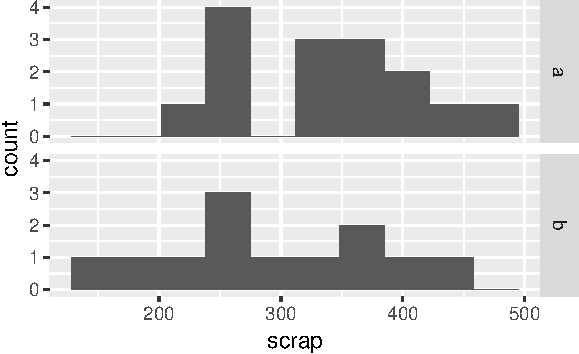
\includegraphics{02-reading-in_files/figure-latex/unnamed-chunk-15-1}

I could have used \texttt{facet\_wrap}, but that would have put the
histograms side by side, and I wanted them one above the other (for ease
of comparison, since they'll be on the same scale). \texttt{facet\_grid}
is like \texttt{facet\_wrap}, but offers you more control over where the
facets go: you can arrange them above and below by a variable, or left
and right by a variable. Whatever is facetting the plots up and down (on
the \(y\) axis) goes before the squiggle, and whatever facets them left
and right goes after. If there is nothing separating the facets in one
direction, here horizontally, the variable is replaced by a dot.

In some ways, \texttt{facet\_grid} is also \emph{less} flexible, because
the facets have to be arranged up/down or left/right by a variable. That
worked here, but if you think back to the Australian athletes, where
there were ten different sports, it was \texttt{facet\_wrap} that did
the right thing, arranging the sports along rows \emph{and} columns to
produce a pleasing display.

All right, that bimodality. I was expecting that the scrap values from
one line would be centred about one value and the scrap values from the
other line would be centred about a different value, with a gap in
between. But that's not what happened at all: the line B values are all
over the place, while it's the line A values that are actually bimodal
all by themselves. I'm not sure whether that really means anything,
since the data sets are pretty small, but it's kind of interesting.

\begin{enumerate}
\def\labelenumi{(\alph{enumi})}
\setcounter{enumi}{5}
\tightlist
\item
  We started out with the suspicion that if the line was run faster,
  there would be more scrap. We haven't assessed this yet. Draw a
  scatter plot with \texttt{scrap} on the \(y\) axis and \texttt{speed}
  on the \(x\) axis.
\end{enumerate}

Solution

Same mechanism as before:

\begin{Shaded}
\begin{Highlighting}[]
\KeywordTok{ggplot}\NormalTok{(soap, }\KeywordTok{aes}\NormalTok{(}\DataTypeTok{x =}\NormalTok{ speed, }\DataTypeTok{y =}\NormalTok{ scrap)) }\OperatorTok{+}\StringTok{ }\KeywordTok{geom_point}\NormalTok{()}
\end{Highlighting}
\end{Shaded}

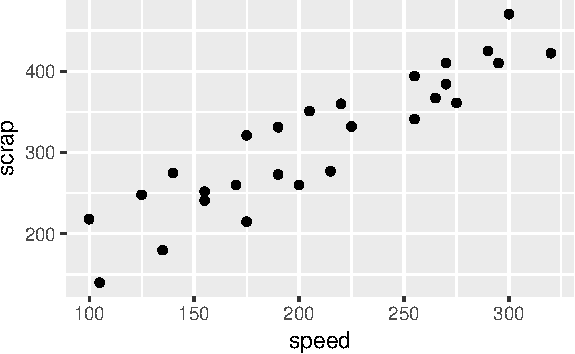
\includegraphics{02-reading-in_files/figure-latex/unnamed-chunk-16-1}

\begin{enumerate}
\def\labelenumi{(\alph{enumi})}
\setcounter{enumi}{6}
\tightlist
\item
  What do you think is the most important conclusion from your plot of
  the previous part? Describe your conclusion in the context of the
  data.
\end{enumerate}

Solution

There seems to be a pretty evident upward trend, apparently linear,
which means that if the speed of the production line is higher, the
amount of scrap produced is also higher. My last sentence was meant to
remind you that ``there is an upward trend'' is \emph{not a complete
answer}: we are concerned with what that upward trend tells us about the
data. This, in other words, confirms the suspicion expressed in the
question, which was therefore a rather large clue: more speed tends to
go with more scrap. That was as far as I wanted you to go: there seems
to be an association with speed, and there might be an association with
\texttt{line} that turned out not to be statistically significant. What
we haven't done is to assess the relationship between speed and scrap
for \emph{each} production line. To do that, we want to plot the
scrap-speed points distinguished for each production line.
\texttt{ggplot} makes that easy: you add a \texttt{colour}
\marginnote{If you are concerned about the spelling: the guy who wrote ggplot is from New Zealand, where they spell *colour* the same way we do. However, if you want to use *color*, that works too.}
to say what you want to distinguish by colour. This is two quantitative
variables and one categorical variable, if you want to think of it that
way:

\begin{Shaded}
\begin{Highlighting}[]
\KeywordTok{ggplot}\NormalTok{(soap, }\KeywordTok{aes}\NormalTok{(}\DataTypeTok{x =}\NormalTok{ speed, }\DataTypeTok{y =}\NormalTok{ scrap, }\DataTypeTok{colour =}\NormalTok{ line)) }\OperatorTok{+}\StringTok{ }
\StringTok{    }\KeywordTok{geom_point}\NormalTok{()}
\end{Highlighting}
\end{Shaded}

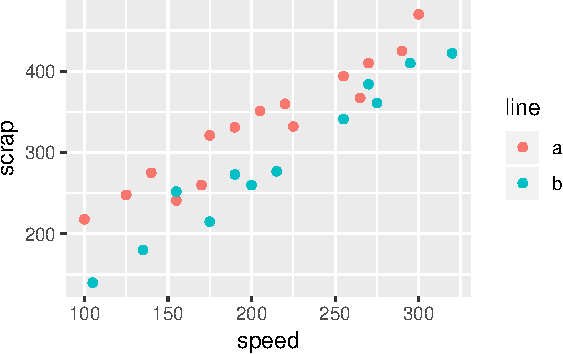
\includegraphics{02-reading-in_files/figure-latex/unnamed-chunk-17-1}

Notice that we get a legend, automatically.

What is interesting about this one is the red dots are mostly at the top
(for any given speed), and the blue dots are mostly at the bottom. That
seems to mean that \emph{when we account for speed}, there is a
difference between lines.

I want to show you one more embellishment, which is to put the
regression lines on the plot for each group separately. This is where
\texttt{ggplot} is so nice, since I just have to add one thing:

\begin{Shaded}
\begin{Highlighting}[]
\KeywordTok{ggplot}\NormalTok{(soap, }\KeywordTok{aes}\NormalTok{(}\DataTypeTok{x =}\NormalTok{ speed, }\DataTypeTok{y =}\NormalTok{ scrap, }\DataTypeTok{colour =}\NormalTok{ line)) }\OperatorTok{+}\StringTok{ }
\StringTok{    }\KeywordTok{geom_point}\NormalTok{() }\OperatorTok{+}\StringTok{ }\KeywordTok{geom_smooth}\NormalTok{(}\DataTypeTok{method =} \StringTok{"lm"}\NormalTok{, }
    \DataTypeTok{se =}\NormalTok{ F)}
\end{Highlighting}
\end{Shaded}

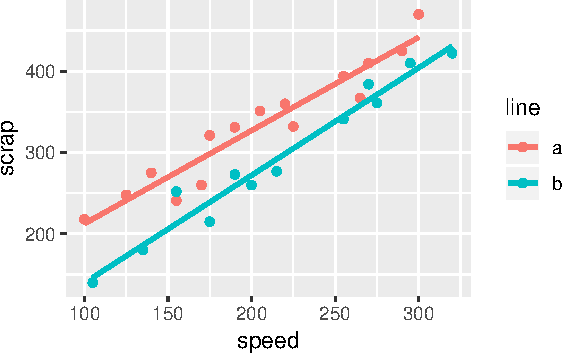
\includegraphics{02-reading-in_files/figure-latex/unnamed-chunk-18-1}

The points and lines have come out in different colours, without our
having to think too hard.

Both lines show an upward trend, with about the same slope, which means
that regardless of line, increasing the speed goes with increasing the
scrap by the same amount. The fact that the red line is above the blue
one, however, suggests that production line A produces more scrap at the
same speed than production line B.

From a management point of view, there is an interesting dynamic at
work: if you run the production line faster, you'll produce more bars of
soap, but you'll produce more scrap as well. The crucial thing for the
people in the supervisor's office is how much raw material is used per
bar of soap, and if you make the soap bars faster, you might use more
raw material, which will eat into your profits (from one angle), but you
will also have more bars of soap to sell.

Here's another way to see the same thing. I'm \emph{definitely} not
expecting you to follow the code, but you can admire the result!

\begin{Shaded}
\begin{Highlighting}[]
\NormalTok{soap2 =}\StringTok{ }\NormalTok{soap }\OperatorTok\StringTok{ }\KeywordTok{select}\NormalTok{(}\OperatorTok{-}\NormalTok{line)}
\KeywordTok{ggplot}\NormalTok{(soap, }\KeywordTok{aes}\NormalTok{(}\DataTypeTok{x =}\NormalTok{ speed, }\DataTypeTok{y =}\NormalTok{ scrap)) }\OperatorTok{+}\StringTok{ }\KeywordTok{geom_point}\NormalTok{(}\DataTypeTok{data =}\NormalTok{ soap2, }
    \DataTypeTok{colour =} \StringTok{"grey"}\NormalTok{) }\OperatorTok{+}\StringTok{ }\KeywordTok{geom_point}\NormalTok{(}\KeywordTok{aes}\NormalTok{(}\DataTypeTok{colour =}\NormalTok{ line)) }\OperatorTok{+}\StringTok{ }
\StringTok{    }\KeywordTok{facet_wrap}\NormalTok{(}\OperatorTok{~}\NormalTok{line)}
\end{Highlighting}
\end{Shaded}

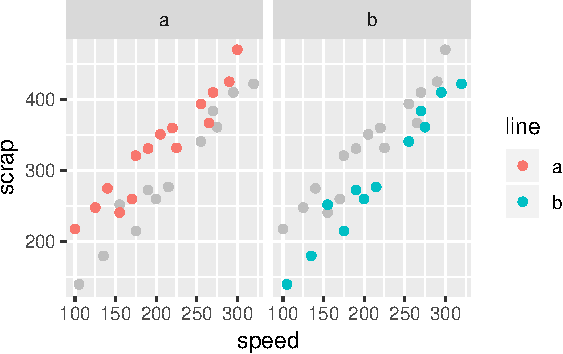
\includegraphics{02-reading-in_files/figure-latex/unnamed-chunk-19-1} \$

The idea is that we plot all the points in grey (to ``put them in the
background'') and then in each plot we plot the points again,
\emph{coloured, for the group we are looking at}: line A in the left,
line B on the right. This is another way of seeing that line A has more
scrap than line B, given the speed at which the line was being run. (I
discovered this technique only yesterday. I think the code is remarkably
concise for what it does.)

The logic of the code is:

\begin{itemize}
\item
  create a new data frame that contains everything in \texttt{soap}
  except for \texttt{line}
\item
  make a scatter plot of all the points in this new data frame, coloured
  grey
\item
  plot the points again (from the original data frame), coloured by
  which production line they're from
\item
  produce a separate scatterplot for each production line.
\end{itemize}

The trick about creating the new data frame was to enable plotting of
all points regardless of group on each subplot (``facet'' in
\texttt{ggplot} terminology), as well as the ones that come from that
production line.

I don't expect you to be able to follow all the details of the code
below, either, but I would like you to try and get the logic. What we do
is a regression predicting \texttt{scrap} from \emph{two} things:
\texttt{speed} and production \texttt{line}. The results we get are
these:

\begin{Shaded}
\begin{Highlighting}[]
\NormalTok{scrap}\FloatTok{.1}\NormalTok{ =}\StringTok{ }\KeywordTok{lm}\NormalTok{(scrap }\OperatorTok{~}\StringTok{ }\NormalTok{speed }\OperatorTok{+}\StringTok{ }\NormalTok{line, }\DataTypeTok{data =}\NormalTok{ soap)}
\KeywordTok{summary}\NormalTok{(scrap}\FloatTok{.1}\NormalTok{)}
\end{Highlighting}
\end{Shaded}

\begin{verbatim}
## 
## Call:
## lm(formula = scrap ~ speed + line, data = soap)
## 
## Residuals:
##     Min      1Q  Median      3Q     Max 
## -39.557 -14.161  -0.121  17.518  33.953 
## 
## Coefficients:
##              Estimate Std. Error t value
## (Intercept)  80.41099   14.54379   5.529
## speed         1.23074    0.06555  18.775
## lineb       -53.12920    8.21003  -6.471
##             Pr(>|t|)    
## (Intercept) 1.10e-05 ***
## speed       7.48e-16 ***
## lineb       1.08e-06 ***
## ---
## Signif. codes:  
##   0 '***' 0.001 '**' 0.01 '*' 0.05 '.' 0.1  ' ' 1
## 
## Residual standard error: 21.13 on 24 degrees of freedom
## Multiple R-squared:  0.9402, Adjusted R-squared:  0.9352 
## F-statistic: 188.6 on 2 and 24 DF,  p-value: 2.104e-15
\end{verbatim}

The P-values for \texttt{speed} and \texttt{line} are the second and
third things in the last column, \(7 \times 10^{-16}\) and
\(1 \times 10^{-6}\) respectively. These are both very strongly
significant, in contrast to the two-sample \(t\)-test where
\texttt{line} was not significant.

So does production line make a difference or not?

The plot says that it does, and the meaning of model \texttt{scrap.1}
just above is that \emph{`speed` affects scrap when you account
for `line`}, and emph\{\texttt{line} affects scrap when you account for
speed\}. (In the two-sample \(t\)-test above we didn't account for speed
at all, since the various speeds were all mixed up.)

There is a moral to this story, which I would like you to get even if
you don't get any of the statistics: if a variable makes a difference,
it should be in your model and on your graph,
\marginnote{Meaning that the graph should contain all three variables, *speed*, *scrap* and *line*.}
because it enables you to get better (more precise) conclusions about
your other variables. Here, there really is a difference between the
production lines, but the \(t\)-test was too much of a blunt instrument
to unearth it (because \texttt{speed} made a difference as well).

\hypertarget{handling-shipments}{%
\section{Handling shipments}\label{handling-shipments}}

A company called Global Electronics from time to time imports shipments
of a certain large part used as a component in several of its products.
The size of the shipment varies each time. Each shipment is sent to one
of two warehouses (labelled A and B) for handling. The data in
\href{http://www.utsc.utoronto.ca/~butler/c32/global.csv}{link} show the
\texttt{size} of each shipment (in thousands of parts) and the direct
\texttt{cost} of handling it, in thousands of dollars. Also shown is the
\texttt{warehouse} (A or B) that handled each shipment.

\begin{enumerate}
\def\labelenumi{(\alph{enumi})}
\tightlist
\item
  Read the data into R and display your data frame. How many rows and
  columns does it have?
\end{enumerate}

Solution

If you open the data file in your web browser, it will probably open as
a spreadsheet, which is not really very helpful, since then it is not
clear what to do with it. You could, I suppose, save it and upload it to
R Studio Cloud, but it requires much less brainpower to open it directly
from the URL:

\begin{Shaded}
\begin{Highlighting}[]
\NormalTok{url =}\StringTok{ "http://www.utsc.utoronto.ca/~butler/c32/global.csv"}
\NormalTok{shipments =}\StringTok{ }\KeywordTok{read_csv}\NormalTok{(url)}
\end{Highlighting}
\end{Shaded}

\begin{verbatim}
## Parsed with column specification:
## cols(
##   warehouse = col_character(),
##   size = col_integer(),
##   cost = col_double()
## )
\end{verbatim}

If you display your data frame and it looks like this, you are good (you
can give the data frame any name):

\begin{Shaded}
\begin{Highlighting}[]
\NormalTok{shipments}
\end{Highlighting}
\end{Shaded}

\begin{verbatim}
## # A tibble: 10 x 3
##    warehouse  size  cost
##    <chr>     <int> <dbl>
##  1 A           225 12.0 
##  2 B           350 14.1 
##  3 A           150  8.93
##  4 A           200 11.0 
##  5 A           175 10.0 
##  6 A           180 10.1 
##  7 B           325 13.8 
##  8 B           290 13.3 
##  9 B           400 15   
## 10 A           125  7.97
\end{verbatim}

It has 10 rows and 3 columns. \emph{You need to say this to get the
mark.}

That is, there were 10 shipments recorded, and for each of them, 3
variables were noted: the size and cost of the shipment, and the
warehouse it was handled at.

\begin{enumerate}
\def\labelenumi{(\alph{enumi})}
\setcounter{enumi}{1}
\tightlist
\item
  Make a scatterplot of the cost of handling each shipment as it depends
  on the shipment's size.
\end{enumerate}

Solution

The wording of the question says that cost is the response and so
belongs on the \(y\)-axis. To make the plot, \texttt{ggplot} with an
\texttt{x=} and a \texttt{y=} in the \texttt{aes} (the ``what to plot''
part), and a \texttt{geom\_point()} after (the ``how to plot it''):

\begin{Shaded}
\begin{Highlighting}[]
\KeywordTok{ggplot}\NormalTok{(shipments, }\KeywordTok{aes}\NormalTok{(}\DataTypeTok{x =}\NormalTok{ size, }\DataTypeTok{y =}\NormalTok{ cost)) }\OperatorTok{+}\StringTok{ }\KeywordTok{geom_point}\NormalTok{()}
\end{Highlighting}
\end{Shaded}

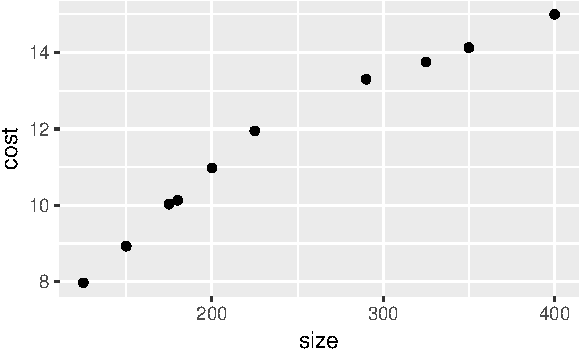
\includegraphics{02-reading-in_files/figure-latex/unnamed-chunk-23-1}

As a matter of coding, there are usually \emph{two} brackets to close
after the \texttt{aes}, the one that begins the \texttt{ggplot} and the
one that begins the \texttt{aes}.

\begin{enumerate}
\def\labelenumi{(\alph{enumi})}
\setcounter{enumi}{2}
\tightlist
\item
  What kind of relationship do you see on the scatterplot? Do you think
  a straight line would describe it appropriately? Explain briefly.
\end{enumerate}

Solution

I see an upward trend: a shipment with larger \texttt{size} costs more
to handle. If you look carefully at the scatterplot, you see that the
cost of handling a small shipment goes up fairly steeply with its size,
but the cost of handling a large shipment, while it still increases with
\texttt{size}, does not increase so fast. Thus having one straight line
to describe the whole relationship would not work so well. The
relationship is actually two different straight lines joined end-to-end,
which we will explore later, but if you think the relationship is
curved, I'll accept that. The point is to get at the idea that the rate
of increase is not constant.

\begin{enumerate}
\def\labelenumi{(\alph{enumi})}
\setcounter{enumi}{3}
\tightlist
\item
  When a shipment comes in, the cost of handling it is not known. A
  decision is made about which warehouse to send it to, and then, after
  it is handled, the cost is recorded. What do you think determines
  which warehouse an incoming shipment goes to? Provide a graph to
  support your answer.
\end{enumerate}

Solution

The veiled hint in the question is that the decision must depend on
\texttt{size}, since it cannot depend on \texttt{cost}. So we have one
quantitative variable \texttt{size} and one categorical variable
\texttt{warehouse}, which suggests drawing boxplots:

\begin{Shaded}
\begin{Highlighting}[]
\KeywordTok{ggplot}\NormalTok{(shipments, }\KeywordTok{aes}\NormalTok{(}\DataTypeTok{x =}\NormalTok{ warehouse, }\DataTypeTok{y =}\NormalTok{ size)) }\OperatorTok{+}\StringTok{ }
\StringTok{    }\KeywordTok{geom_boxplot}\NormalTok{()}
\end{Highlighting}
\end{Shaded}

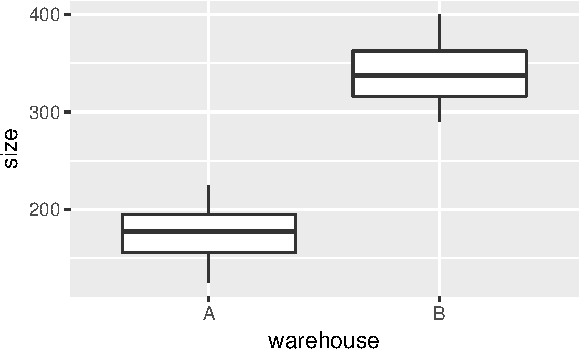
\includegraphics{02-reading-in_files/figure-latex/unnamed-chunk-24-1}

Well, there's the answer right there. When the shipment has small
\texttt{size}, it goes to warehouse A, and when it's large, it goes to
Warehouse B. We know this because \emph{all} the shipments smaller than
about 250 (thousand parts) went to A and \emph{all} the shipments larger
than that went to B. (If you want to provide a number to delineate
``small'' and ``large'', anything between the largest A, about 225, and
the smallest B, about 290, will do.)

Another way to think about this is to add something to the scatterplot
you drew before. The obvious thing is to make the two warehouses
different colours:

\begin{Shaded}
\begin{Highlighting}[]
\KeywordTok{ggplot}\NormalTok{(shipments, }\KeywordTok{aes}\NormalTok{(}\DataTypeTok{x =}\NormalTok{ size, }\DataTypeTok{y =}\NormalTok{ cost, }\DataTypeTok{colour =}\NormalTok{ warehouse)) }\OperatorTok{+}\StringTok{ }
\StringTok{    }\KeywordTok{geom_point}\NormalTok{()}
\end{Highlighting}
\end{Shaded}

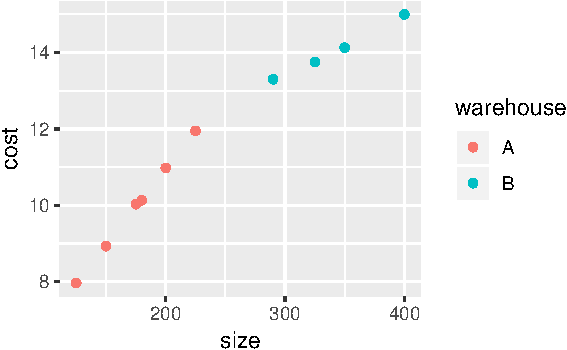
\includegraphics{02-reading-in_files/figure-latex/unnamed-chunk-25-1}

As a point of technique, you can split lines of code to make them fit on
your screen. You can do this as long as \emph{the code that ends
the line must be incomplete}, so that R knows more is to come. Ending a
line with a pipe symbol, or, as here, with one of the pluses in the
middle of a \texttt{ggplot}, will work. If you put the plus on the start
of the next line, you'll get a blank plot, because R thinks you're done
plotting. Try it and see.

Anyway, this plot tells exactly the same story: the small shipments (in
size or cost) go to Warehouse A and the large ones to Warehouse B. But
we don't know cost when the decision is made about which warehouse to
send a shipment to, so the decision must be based on \texttt{size}.

In the place where I got these data, it said ``larger shipments are sent
to Warehouse B, since this warehouse has specialized equipment that
provides greater economies of scale for larger shipments''. That is to
say, very large shipments are more expensive to handle, but not as
expensive as you might think.
\marginnote{This is the same idea that it  costs more to ride the GO bus from UTSC to York U than it does to  ride from UTSC to Scarborough Town, but if you work out how much it  costs per kilometre, the longer journey costs less per km. As of  when I'm writing this, $5.30 for the 7.2 km to Scarborough Town and  $6.75 for the 38 km to York. That's quite an economy of scale,  isn't it?}
That makes sense with our scatterplot, because the \emph{slope} for
larger shipments is less than for smaller shipments.

When we get to regression later, we'll see what happens if we fit a
straight line to data like these, and how to tell whether we really
ought to be able to do better with a different form of relationship.
There is also a trick to fit what is called a ``piecewise linear
regression'', which has one slope for small shipment sizes, a different
(smaller) slope for large ones, and joins up in the middle. But that's
well beyond our scope now.

\hypertarget{data-exploration}{%
\chapter{Data exploration}\label{data-exploration}}

\begin{Shaded}
\begin{Highlighting}[]
\KeywordTok{library}\NormalTok{(tidyverse)}
\end{Highlighting}
\end{Shaded}

\begin{verbatim}
## -- Attaching packages ---- tidyverse 1.2.1 --
\end{verbatim}

\begin{verbatim}
## v ggplot2 3.0.0     v purrr   0.2.5
## v tibble  1.4.2     v dplyr   0.7.6
## v tidyr   0.8.1     v stringr 1.3.1
## v readr   1.1.1     v forcats 0.3.0
\end{verbatim}

\begin{verbatim}
## -- Conflicts ------- tidyverse_conflicts() --
## x dplyr::filter() masks stats::filter()
## x dplyr::lag()    masks stats::lag()
\end{verbatim}

\hypertarget{north-carolina-births}{%
\section{North Carolina births}\label{north-carolina-births}}

The data in file
\href{http://www.utsc.utoronto.ca/~butler/c32/ncbirths.csv}{link} are
about 500 randomly chosen births of babies in North Carolina. There is a
lot of information: not just the weight at birth of the baby, but
whether the baby was born prematurely, the ages of the parents, whether
the parents are married, how long (in weeks) the pregnancy lasted (this
is called the ``gestation'') and so on.

\begin{enumerate}
\def\labelenumi{(\alph{enumi})}
\tightlist
\item
  Read in the data from the file into R, bearing in mind what type of
  file it is.
\end{enumerate}

Solution

This is a \texttt{.csv} file (it came from a spreadsheet), so it needs
reading in accordingly. Work directly from the URL (rather than
downloading the file, unless you are working offline):

\begin{Shaded}
\begin{Highlighting}[]
\NormalTok{myurl =}\StringTok{ "http://www.utsc.utoronto.ca/~butler/c32/ncbirths.csv"}
\NormalTok{bw =}\StringTok{ }\KeywordTok{read_csv}\NormalTok{(myurl)}
\end{Highlighting}
\end{Shaded}

\begin{verbatim}
## Parsed with column specification:
## cols(
##   `Father Age` = col_integer(),
##   `Mother Age` = col_integer(),
##   `Weeks Gestation` = col_integer(),
##   `Pre-natal Visits` = col_integer(),
##   `Marital Status` = col_integer(),
##   `Mother Weight Gained` = col_integer(),
##   `Low Birthweight?` = col_integer(),
##   `Weight (pounds)` = col_double(),
##   `Premie?` = col_integer(),
##   `Few Visits?` = col_integer()
## )
\end{verbatim}

This shows you which variables the data set has (some of the names got a
bit mangled), and it shows you that they are all integers except for the
birth weight (a decimal number).

The easiest way to find out how many rows and columns there are is
simply to list the data frame:

\begin{Shaded}
\begin{Highlighting}[]
\NormalTok{bw}
\end{Highlighting}
\end{Shaded}

\begin{verbatim}
## # A tibble: 500 x 10
##    `Father Age` `Mother Age` `Weeks Gestatio~
##           <int>        <int>            <int>
##  1           27           26               38
##  2           35           33               40
##  3           34           22               37
##  4           NA           16               38
##  5           35           33               39
##  6           32           24               36
##  7           33           33               38
##  8           38           35               38
##  9           28           29               40
## 10           NA           19               34
## # ... with 490 more rows, and 7 more
## #   variables: `Pre-natal Visits` <int>,
## #   `Marital Status` <int>, `Mother Weight
## #   Gained` <int>, `Low Birthweight?` <int>,
## #   `Weight (pounds)` <dbl>,
## #   `Premie?` <int>, `Few Visits?` <int>
\end{verbatim}

or you can take a ``glimpse'' of it:

\begin{Shaded}
\begin{Highlighting}[]
\KeywordTok{glimpse}\NormalTok{(bw)}
\end{Highlighting}
\end{Shaded}

\begin{verbatim}
## Observations: 500
## Variables: 10
## $ `Father Age`           <int> 27, 35, 3...
## $ `Mother Age`           <int> 26, 33, 2...
## $ `Weeks Gestation`      <int> 38, 40, 3...
## $ `Pre-natal Visits`     <int> 14, 11, 1...
## $ `Marital Status`       <int> 1, 1, 2, ...
## $ `Mother Weight Gained` <int> 32, 23, 5...
## $ `Low Birthweight?`     <int> 0, 0, 0, ...
## $ `Weight (pounds)`      <dbl> 6.8750, 6...
## $ `Premie?`              <int> 0, 0, 0, ...
## $ `Few Visits?`          <int> 0, 0, 0, ...
\end{verbatim}

Either of these displays show that there are 500 rows (observations,
here births) and 10 columns (variables), and they both show what the
variables are called. So they're both good as an answer to the question.

What you'll notice is that the variables have \emph{spaces} in their
names, which will require special handling later. These outputs show you
what to do about those spaces in variable names: surround the variable
name with ``backticks''. (On my keyboard, that's on the key to the left
of number 1, where the squiggle is, that looks like a backwards
apostrophe. Probably next to \texttt{Esc}, depending on the layout of
your keyboard.)

Although almost all of the variables are stored as integers, the ones
that have a question mark in their name are actually ``logical'', true
or false, with 1 denoting true and 0 false. We could convert them later
if we want to. (A question mark is not a traditional character to put in
a variable name, so we have to surround these variables with backticks
too.)

\begin{enumerate}
\def\labelenumi{(\alph{enumi})}
\setcounter{enumi}{1}
\tightlist
\item
  From your output, verify that you have the right number of
  observations and that you have several variables. Which of your
  variables correspond to birthweight, prematureness and length of
  pregnancy? (You might have to make guesses based on the names of the
  variables.)
\end{enumerate}

Solution

I do indeed have 500 observations on 10 variables (``several''). (If you
don't have several variables, check to see that you didn't use
\texttt{read\_delim} or something by mistake.) After the ``500
observations of 10 variables'' line(s) in each case, you see all the
variables by name, with what type of values they have,
\marginnote{these    are mostly *int* or *integer*.} and the first few
of the values.
\marginnote{Other possible variable types are *num* for    (real, decimal) numbers such as birth weight, *chr* for    text, and *Factor* (with the number of levels) for    factors/categorical variables. We don't have any of the last two    here. There is also *lgl* for *logical*, things that were    actually recorded as TRUE or FALSE. We have some variables that    are actually logical ones, but they are recorded as integer    values.}

The variable \texttt{Weight\ (pounds)} is the birthweight (in pounds),
\texttt{Premie?} is 1 for a premature baby and 0 for a full-term baby,
and \texttt{Weeks\ Gestation} is the number of weeks the pregnancy
lasted. Don't forget to put backticks around each of those when you use
them later.
\marginnote{The backticks look different from each other for  annoying technical reasons, but they're all backticks.}

\begin{enumerate}
\def\labelenumi{(\alph{enumi})}
\setcounter{enumi}{2}
\tightlist
\item
  The theory behind the \(t\)-test (which we do later) says that the
  distribution of birth weights should be (approximately) normally
  distributed. Obtain a histogram of the birth weights. Does it look
  approximately normal? Comment briefly. (You'll have to pick a number
  of bins for your histogram first. I don't mind very much what you
  pick, as long as it's not obviously too many or too few bins.)
\end{enumerate}

Solution

You'll have seen that I often start with 10 bins, or maybe not quite
that many if I don't have much data, and this is a decent general
principle. That would give

\begin{Shaded}
\begin{Highlighting}[]
\KeywordTok{ggplot}\NormalTok{(bw, }\KeywordTok{aes}\NormalTok{(}\DataTypeTok{x =} \StringTok{`}\DataTypeTok{Weight (pounds)}\StringTok{`}\NormalTok{)) }\OperatorTok{+}\StringTok{ }\KeywordTok{geom_histogram}\NormalTok{(}\DataTypeTok{bins =} \DecValTok{10}\NormalTok{)}
\end{Highlighting}
\end{Shaded}

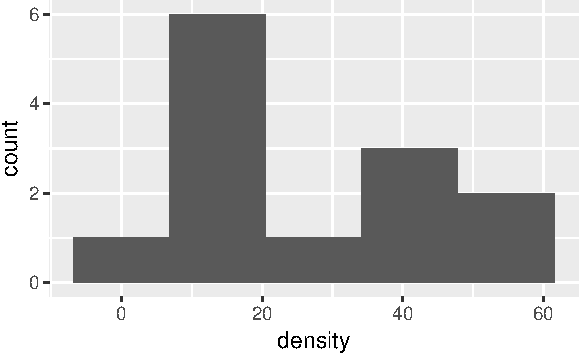
\includegraphics{03-data-summaries_files/figure-latex/unnamed-chunk-9-1}

which is perfectly acceptable. You can try something a bit more or a bit
less, and see how you like it in comparison. What you are looking for is
a nice clear picture of \emph{shape}. If you have too few bins, you'll
lose the shape:

\begin{Shaded}
\begin{Highlighting}[]
\KeywordTok{ggplot}\NormalTok{(bw, }\KeywordTok{aes}\NormalTok{(}\DataTypeTok{x =} \StringTok{`}\DataTypeTok{Weight (pounds)}\StringTok{`}\NormalTok{)) }\OperatorTok{+}\StringTok{ }\KeywordTok{geom_histogram}\NormalTok{(}\DataTypeTok{bins =} \DecValTok{4}\NormalTok{)}
\end{Highlighting}
\end{Shaded}

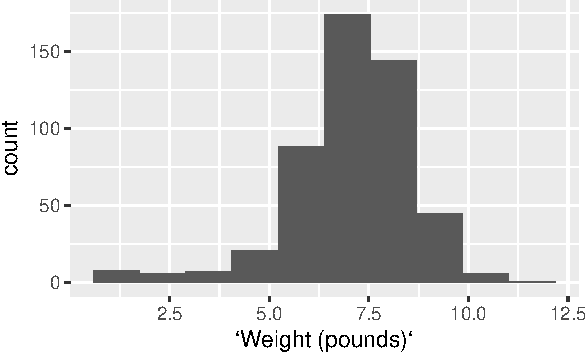
\includegraphics{03-data-summaries_files/figure-latex/unnamed-chunk-10-1}

(is that leftmost bin an indication of skewness or some observations
that happen to be smallish?)

And if you have too many, the shape will be there, but it will be hard
to make out in all the noise, with frequencies going up and down:

\begin{Shaded}
\begin{Highlighting}[]
\KeywordTok{ggplot}\NormalTok{(bw, }\KeywordTok{aes}\NormalTok{(}\DataTypeTok{x =} \StringTok{`}\DataTypeTok{Weight (pounds)}\StringTok{`}\NormalTok{)) }\OperatorTok{+}\StringTok{ }\KeywordTok{geom_histogram}\NormalTok{(}\DataTypeTok{bins =} \DecValTok{30}\NormalTok{)}
\end{Highlighting}
\end{Shaded}

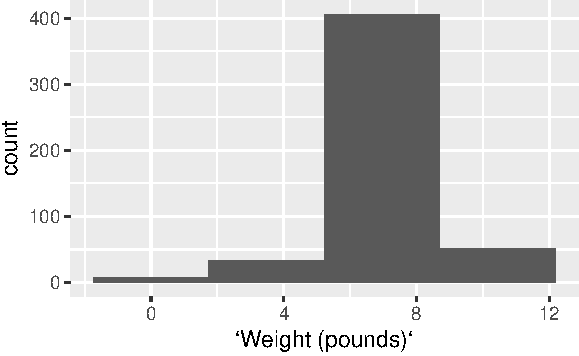
\includegraphics{03-data-summaries_files/figure-latex/unnamed-chunk-11-1}

I generally am fairly relaxed about the number of bins you use, as long
as it's not clearly too few or too many. You might have done exercises
in the past that illustrate that the choice of number of bins (or the
class intervals where you move from one bin to the next, which is
another issue that I won't explore here) can make an appreciable
difference to how a histogram looks. Extra: I had some thoughts about
this issue that I put in a blog post, that you might like to read:
\href{http://ritsokiguess.site/docs/2017/06/08/histograms-and-bins/}{link}.
The nice thing about Sturges' rule, mentioned there, is that you can
almost get a number of bins for your histogram in your head (as long as
you know the powers of 2, that is). What you do is to start with your
sample size, here \(n=500\). You find the next power of 2 above that,
which is here \(512=2^9\). You then take that power and add 1, to get 10
bins. If you don't like that, you can get R to calculate it for you:

\begin{Shaded}
\begin{Highlighting}[]
\KeywordTok{nclass.Sturges}\NormalTok{(bw}\OperatorTok{$}\StringTok{`}\DataTypeTok{Weight (pounds)}\StringTok{`}\NormalTok{)}
\end{Highlighting}
\end{Shaded}

\begin{verbatim}
## [1] 10
\end{verbatim}

The place where Sturges' rule comes from is an assumption of normal data
(actually a binomial approximation to the normal, backwards though that
sounds). If you have less than 30 observations, you'll get fewer than 6
bins, which won't do much of a job of showing the shape. Rob Hyndman
wrote a \href{https://robjhyndman.com/papers/sturges.pdf}{critical note}
about Sturges' rule in which he asserts that it is just plain wrong (if
you have taken B57, this note is very readable).

So what to use instead? Well, judgment is still better than something
automatic, but if you want a place to start from, something with a
better foundation than Sturges is the Freedman-Diaconis rule. This, in
its original formulation, gives a bin width rather than a number of
bins:

\[ 
w=2(IQR)n^{-1/3}
\]

The nice thing about this is that it uses the interquartile range, so it
won't be distorted by outliers. \texttt{geom\_histogram} can take a bin
width, so we can use it as follows:

\begin{Shaded}
\begin{Highlighting}[]
\NormalTok{w =}\StringTok{ }\DecValTok{2} \OperatorTok{*}\StringTok{ }\KeywordTok{IQR}\NormalTok{(bw}\OperatorTok{$}\StringTok{`}\DataTypeTok{Weight (pounds)}\StringTok{`}\NormalTok{) }\OperatorTok{*}\StringTok{ }\DecValTok{500}\OperatorTok{^}\NormalTok{(}\OperatorTok{-}\DecValTok{1}\OperatorTok{/}\DecValTok{3}\NormalTok{)}
\NormalTok{w}
\end{Highlighting}
\end{Shaded}

\begin{verbatim}
## [1] 0.4094743
\end{verbatim}

\begin{Shaded}
\begin{Highlighting}[]
\KeywordTok{ggplot}\NormalTok{(bw, }\KeywordTok{aes}\NormalTok{(}\DataTypeTok{x =} \StringTok{`}\DataTypeTok{Weight (pounds)}\StringTok{`}\NormalTok{)) }\OperatorTok{+}\StringTok{ }\KeywordTok{geom_histogram}\NormalTok{(}\DataTypeTok{binwidth =}\NormalTok{ w)}
\end{Highlighting}
\end{Shaded}

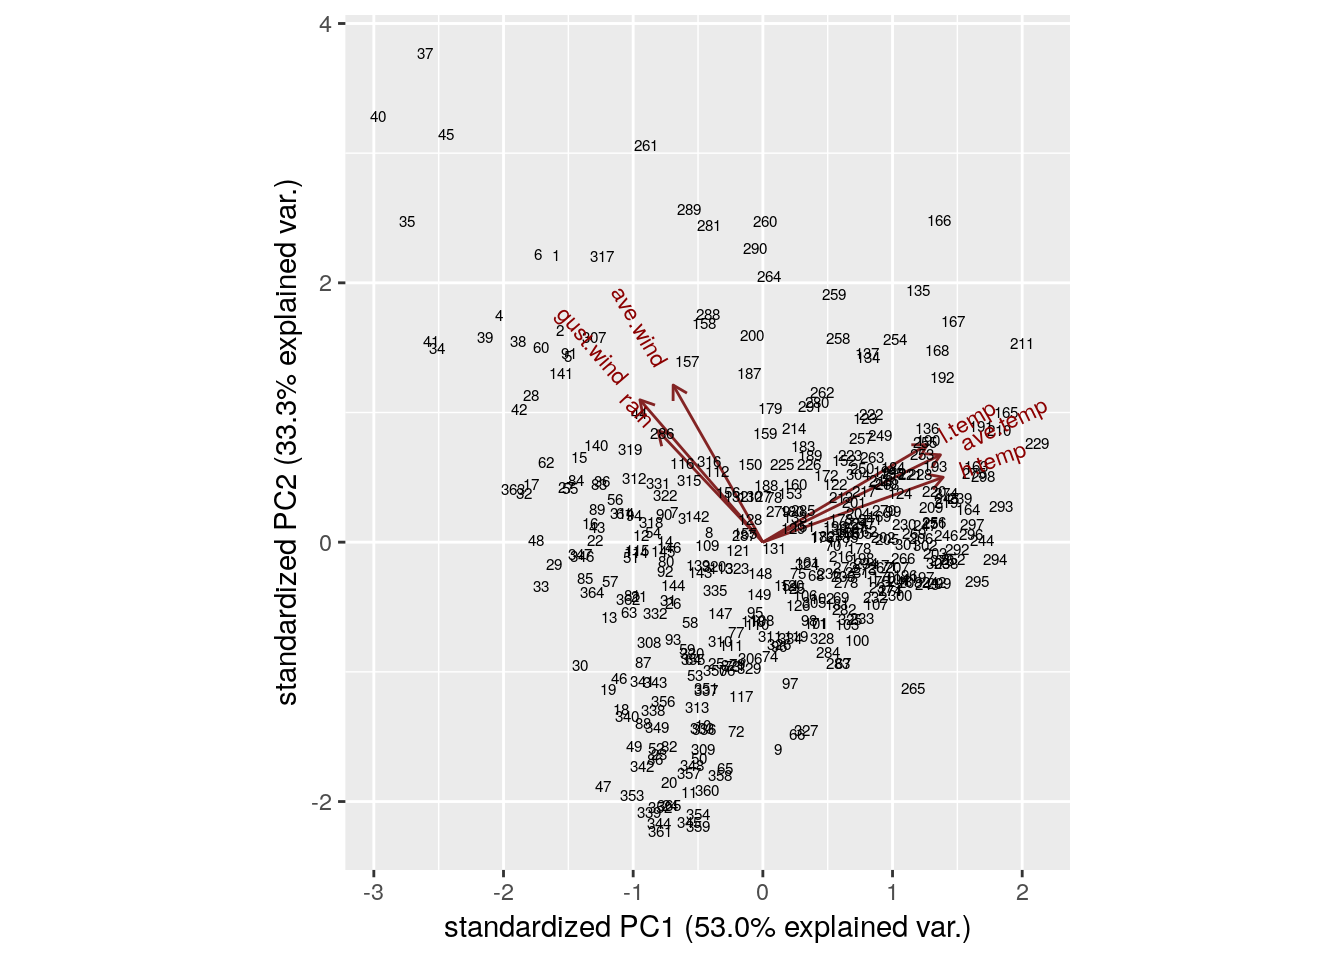
\includegraphics{03-data-summaries_files/figure-latex/unnamed-chunk-13-1}

R also has

\begin{Shaded}
\begin{Highlighting}[]
\NormalTok{nc =}\StringTok{ }\KeywordTok{nclass.FD}\NormalTok{(bw}\OperatorTok{$}\StringTok{`}\DataTypeTok{Weight (pounds)}\StringTok{`}\NormalTok{)}
\NormalTok{nc}
\end{Highlighting}
\end{Shaded}

\begin{verbatim}
## [1] 26
\end{verbatim}

which turns the Freedman-Diaconis rule into a number of bins rather than
a binwidth; using that gives the same histogram as we got with
\texttt{binwidth}.

In my opinion, Freedman-Diaconis tends to give too many bins (here there
are 26 rather than the 10 of Sturges). But I put it out there for you to
make your own call.

Another way to go is a ``density plot''. This is a smoothed-out version
of a histogram that is not obviously frequencies in bins, but which does
have a theoretical basis. It goes something like this:

\begin{Shaded}
\begin{Highlighting}[]
\KeywordTok{ggplot}\NormalTok{(bw, }\KeywordTok{aes}\NormalTok{(}\DataTypeTok{x =} \StringTok{`}\DataTypeTok{Weight (pounds)}\StringTok{`}\NormalTok{)) }\OperatorTok{+}\StringTok{ }\KeywordTok{geom_density}\NormalTok{()}
\end{Highlighting}
\end{Shaded}

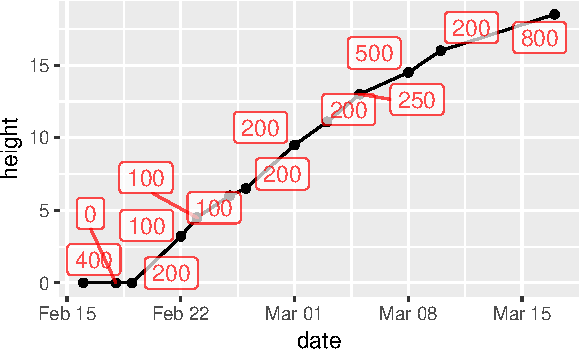
\includegraphics{03-data-summaries_files/figure-latex/unnamed-chunk-15-1}

\texttt{geom\_density} has an optional parameter that controls how
smooth or wiggly the picture is, but the default is usually good.

Alright, before we got distracted, we were assessing normality. What
about that?

It is mostly normal-looking, but I am suspicious about those \emph{very}
low birth weights, the ones below about 4 pounds. There are a few too
many of those, as I see it.

If you think this is approximately normal, you need to make some comment
along the lines of ``the shape is approximately symmetric with no
outliers''. I think my first answer is better, but this answer is worth
something, since it is a not completely unreasonable interpretation of
the histogram.

I have been making the distinction between a histogram (for one
quantitative variable) and side-by-side boxplots (for one quantitative
variable divided into groups by one categorical variable). When you
learned the boxplot, you probably learned it in the context of one
quantitative variable. You can draw a boxplot for that, too, but the
\texttt{ggplot} boxplot has an \texttt{x} as well as a \texttt{y}. What
you do to make a single boxplot is to set the \texttt{x} equal 1, which
produces a weird \(x\)-axis (that you ignore):

\begin{Shaded}
\begin{Highlighting}[]
\KeywordTok{ggplot}\NormalTok{(bw, }\KeywordTok{aes}\NormalTok{(}\DataTypeTok{x =} \DecValTok{1}\NormalTok{, }\DataTypeTok{y =} \StringTok{`}\DataTypeTok{Weight (pounds)}\StringTok{`}\NormalTok{)) }\OperatorTok{+}\StringTok{ }
\StringTok{    }\KeywordTok{geom_boxplot}\NormalTok{()}
\end{Highlighting}
\end{Shaded}

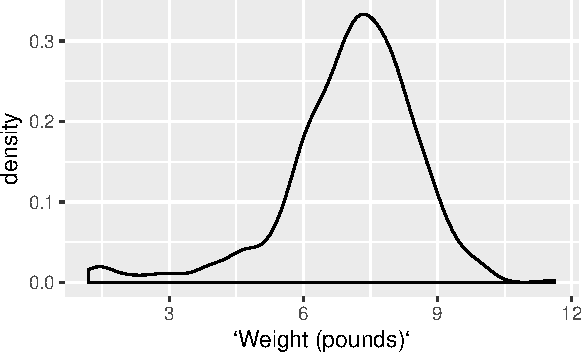
\includegraphics{03-data-summaries_files/figure-latex/unnamed-chunk-16-1}

The high weight is actually an outlier, but look at all those outliers
at the bottom!
\marginnote{When Tukey, a name we will see again, invented  the boxplot in the 1950s, 500 observations would have been  considered a big data set. He designed the boxplot to produce a  sensible number of outliers for the typical size of data set of his  day, but a boxplot of a large data set tends to have a lot of  outliers that are probably not really outliers at all.}

\emph{I} think the reason for those extra very low values is that they
are the premature births (that can result in \emph{very} small babies).
Which leads to the additional question coming up.

\hypertarget{more-about-the-nc-births}{%
\section{More about the NC births}\label{more-about-the-nc-births}}

This is an exploration of some extra issues around the North Carolina
births data set.

\begin{enumerate}
\def\labelenumi{(\alph{enumi})}
\tightlist
\item
  How short does a pregnancy have to be, for the birth to be classified
  as ``premature''? Deduce this from the data, by drawing a suitable
  graph or otherwise.
\end{enumerate}

Solution

To figure it out from the data, we can see how \texttt{Weeks\ Gestation}
depends on \texttt{Premie?}. Some possibilities are boxplots or a
scatterplot. Either of the first two graphs would get full credit (for
the graphing part: you still have to do the explanation) if this were
being marked:

\begin{Shaded}
\begin{Highlighting}[]
\KeywordTok{ggplot}\NormalTok{(bw, }\KeywordTok{aes}\NormalTok{(}\DataTypeTok{x =} \KeywordTok{factor}\NormalTok{(}\StringTok{`}\DataTypeTok{Premie?}\StringTok{`}\NormalTok{), }\DataTypeTok{y =} \StringTok{`}\DataTypeTok{Weeks Gestation}\StringTok{`}\NormalTok{)) }\OperatorTok{+}\StringTok{ }
\StringTok{    }\KeywordTok{geom_boxplot}\NormalTok{()}
\end{Highlighting}
\end{Shaded}

\begin{verbatim}
## Warning: Removed 1 rows containing non-finite
## values (stat_boxplot).
\end{verbatim}

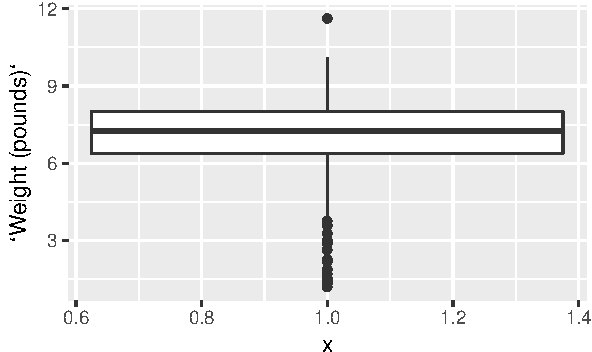
\includegraphics{03-data-summaries_files/figure-latex/unnamed-chunk-17-1}

The warning is because the prematurity of one of the babies is not
known. Or

\begin{Shaded}
\begin{Highlighting}[]
\KeywordTok{ggplot}\NormalTok{(bw, }\KeywordTok{aes}\NormalTok{(}\DataTypeTok{x =} \StringTok{`}\DataTypeTok{Premie?}\StringTok{`}\NormalTok{, }\DataTypeTok{y =} \StringTok{`}\DataTypeTok{Weeks Gestation}\StringTok{`}\NormalTok{)) }\OperatorTok{+}\StringTok{ }
\StringTok{    }\KeywordTok{geom_point}\NormalTok{()}
\end{Highlighting}
\end{Shaded}

\begin{verbatim}
## Warning: Removed 1 rows containing missing values
## (geom_point).
\end{verbatim}

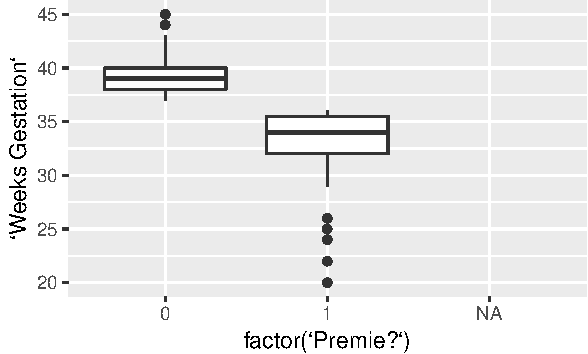
\includegraphics{03-data-summaries_files/figure-latex/unnamed-chunk-18-1}

The same warning again, for the same reason.

Notice how the graphs are similar in syntax, because the what-to-plot is
the same (apart from the \texttt{factor} thing) and we just make a small
change in how-to-plot-it. In the boxplot, the thing on the \(x\)-scale
needs to be categorical, and \texttt{Premie?} is actually a number, so
we'd better make it into a \texttt{factor}, which is R's version of a
categorical variable. \texttt{Premie.} is actually a categorical
variable (``premature'' or ``not premature'') masquerading as a
quantitative one (1 or 0). It is an ``indicator variable'', if you're
familiar with that term.

It looks as if the breakpoint is 37 weeks: a pregnancy at least that
long is considered normal, but a shorter one ends with a premature
birth. Both plots show the same thing: the `\texttt{Premie?}=1` births
all go with short pregnancies, shorter than 37 weeks. This is completely
clear cut.

Another way to attack this is to use \texttt{summarize}, finding the max
and min:

\begin{Shaded}
\begin{Highlighting}[]
\NormalTok{bw }\OperatorTok\StringTok{ }\KeywordTok{summarize}\NormalTok{(}\DataTypeTok{n =} \KeywordTok{n}\NormalTok{(), }\DataTypeTok{min =} \KeywordTok{min}\NormalTok{(}\StringTok{`}\DataTypeTok{Weeks Gestation}\StringTok{`}\NormalTok{), }
    \DataTypeTok{max =} \KeywordTok{max}\NormalTok{(}\StringTok{`}\DataTypeTok{Weeks Gestation}\StringTok{`}\NormalTok{))}
\end{Highlighting}
\end{Shaded}

\begin{verbatim}
## # A tibble: 1 x 3
##       n   min   max
##   <int> <dbl> <dbl>
## 1   500    NA    NA
\end{verbatim}

only this is for \emph{all} the babies, premature or not.
\marginnote{I  explain the missing values below.} So we want it by
prematurity, which means a \texttt{group\_by} first:

\begin{Shaded}
\begin{Highlighting}[]
\NormalTok{bw }\OperatorTok\StringTok{ }\KeywordTok{group_by}\NormalTok{(}\StringTok{`}\DataTypeTok{Premie?}\StringTok{`}\NormalTok{) }\OperatorTok\StringTok{ }\KeywordTok{summarize}\NormalTok{(}\DataTypeTok{n =} \KeywordTok{n}\NormalTok{(), }
    \DataTypeTok{min =} \KeywordTok{min}\NormalTok{(}\StringTok{`}\DataTypeTok{Weeks Gestation}\StringTok{`}\NormalTok{), }\DataTypeTok{max =} \KeywordTok{max}\NormalTok{(}\StringTok{`}\DataTypeTok{Weeks Gestation}\StringTok{`}\NormalTok{))}
\end{Highlighting}
\end{Shaded}

\begin{verbatim}
## # A tibble: 3 x 4
##   `Premie?`     n   min   max
##       <int> <int> <dbl> <dbl>
## 1         0   424    37    45
## 2         1    75    20    36
## 3        NA     1    NA    NA
\end{verbatim}

\texttt{group\_by} with a number works, even though using the number in
\texttt{Premie?} in a boxplot didn't. \texttt{group\_by} just uses the
distinct values, whether they are numbers, text or factor levels.

Any of these graphs or summaries will help you answer the question, in
the same way. The ultimate issue here is ``something that will get the
job done'': it doesn't matter so much what.

In R, \texttt{NA} means ``missing''. When you try to compute something
containing a missing value, the answer is usually missing (since you
don't know what the missing value is). That's why the first
\texttt{summarize} gave us missing values: there was one missing weeks
of gestation in with all the ones for which we had values, so the max
and min had to be missing as well. In the second \texttt{summarize}, the
one by whether a baby was born prematurely or not, we learn a bit more
about that missing \texttt{Premie?}: evidently its weeks of gestation
was missing as well, since the min and max of that were missing.
\marginnote{If there had been a weeks of gestation, we could have figured out whether it was premature or not, according to whether the weeks of gestation was less than 37.}

Here's that baby. I'm doing a bit of fiddling to show all the columns
(as rows, since there's only one actual row). Don't worry about the
second line of code below; we will investigate that later.

\begin{Shaded}
\begin{Highlighting}[]
\NormalTok{bw }\OperatorTok\StringTok{ }\KeywordTok{filter}\NormalTok{(}\KeywordTok{is.na}\NormalTok{(}\StringTok{`}\DataTypeTok{Premie?}\StringTok{`}\NormalTok{)) }\OperatorTok\StringTok{ }\KeywordTok{gather}\NormalTok{(name, }
\NormalTok{    value, }\KeywordTok{everything}\NormalTok{())}
\end{Highlighting}
\end{Shaded}

\begin{verbatim}
## # A tibble: 10 x 2
##    name                 value
##    <chr>                <dbl>
##  1 Father Age           33   
##  2 Mother Age           32   
##  3 Weeks Gestation      NA   
##  4 Pre-natal Visits      9   
##  5 Marital Status        1   
##  6 Mother Weight Gained 25   
##  7 Low Birthweight?      0   
##  8 Weight (pounds)       7.19
##  9 Premie?              NA   
## 10 Few Visits?           0
\end{verbatim}

The \emph{only} thing that was missing was its weeks of gestation, but
that prevented anyone from figuring out whether it was premature or not.

\begin{enumerate}
\def\labelenumi{(\alph{enumi})}
\setcounter{enumi}{1}
\tightlist
\item
  Explore the relationship between birth weight and length of pregancy
  (``gestation'') using a suitable graph. What do you see?
\end{enumerate}

Solution

This needs to be a scatterplot because these are both quantitative
variables:

\begin{Shaded}
\begin{Highlighting}[]
\KeywordTok{ggplot}\NormalTok{(bw, }\KeywordTok{aes}\NormalTok{(}\DataTypeTok{x =} \StringTok{`}\DataTypeTok{Weeks Gestation}\StringTok{`}\NormalTok{, }\DataTypeTok{y =} \StringTok{`}\DataTypeTok{Weight (pounds)}\StringTok{`}\NormalTok{)) }\OperatorTok{+}\StringTok{ }
\StringTok{    }\KeywordTok{geom_point}\NormalTok{()}
\end{Highlighting}
\end{Shaded}

\begin{verbatim}
## Warning: Removed 1 rows containing missing values
## (geom_point).
\end{verbatim}

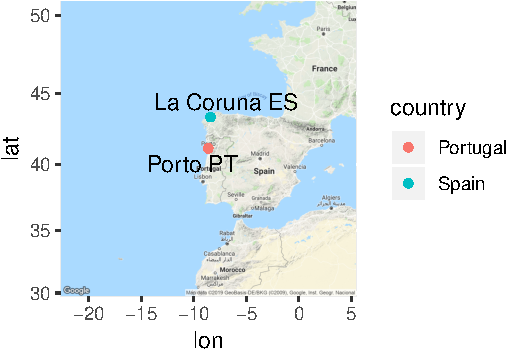
\includegraphics{03-data-summaries_files/figure-latex/unnamed-chunk-22-1}

You see a rather clear upward trend. Those very underweight babies came
from very short pregnancies, but the vast majority of pregnancies were
of more or less normal length (40 weeks is normal) and resulted in
babies of more or less normal birth weight.

I want to illustrate something else: how about \emph{colouring} the
births that were premature? Piece of cake with \texttt{ggplot}:

\begin{Shaded}
\begin{Highlighting}[]
\KeywordTok{ggplot}\NormalTok{(bw, }\KeywordTok{aes}\NormalTok{(}\DataTypeTok{x =} \StringTok{`}\DataTypeTok{Weeks Gestation}\StringTok{`}\NormalTok{, }\DataTypeTok{y =} \StringTok{`}\DataTypeTok{Weight (pounds)}\StringTok{`}\NormalTok{, }
    \DataTypeTok{colour =} \StringTok{`}\DataTypeTok{Premie?}\StringTok{`}\NormalTok{)) }\OperatorTok{+}\StringTok{ }\KeywordTok{geom_point}\NormalTok{()}
\end{Highlighting}
\end{Shaded}

\begin{verbatim}
## Warning: Removed 1 rows containing missing values
## (geom_point).
\end{verbatim}

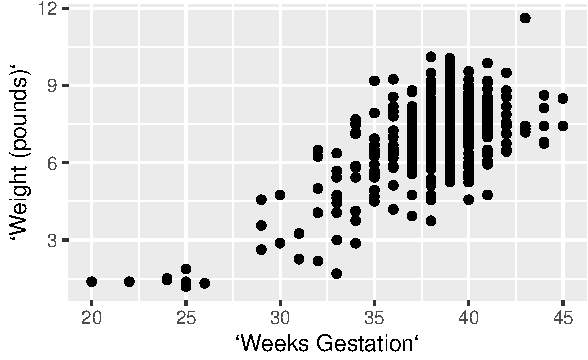
\includegraphics{03-data-summaries_files/figure-latex/unnamed-chunk-23-1}

That was rather silly because \texttt{ggplot} treated prematureness as a
\emph{continuous} variable, and plotted the values on a dark blue-light
blue scale. This is the same issue as on the boxplot above, and has the
same solution:

\begin{Shaded}
\begin{Highlighting}[]
\KeywordTok{ggplot}\NormalTok{(bw, }\KeywordTok{aes}\NormalTok{(}\DataTypeTok{x =} \StringTok{`}\DataTypeTok{Weeks Gestation}\StringTok{`}\NormalTok{, }\DataTypeTok{y =} \StringTok{`}\DataTypeTok{Weight (pounds)}\StringTok{`}\NormalTok{, }
    \DataTypeTok{colour =} \KeywordTok{factor}\NormalTok{(}\StringTok{`}\DataTypeTok{Premie?}\StringTok{`}\NormalTok{))) }\OperatorTok{+}\StringTok{ }\KeywordTok{geom_point}\NormalTok{()}
\end{Highlighting}
\end{Shaded}

\begin{verbatim}
## Warning: Removed 1 rows containing missing values
## (geom_point).
\end{verbatim}

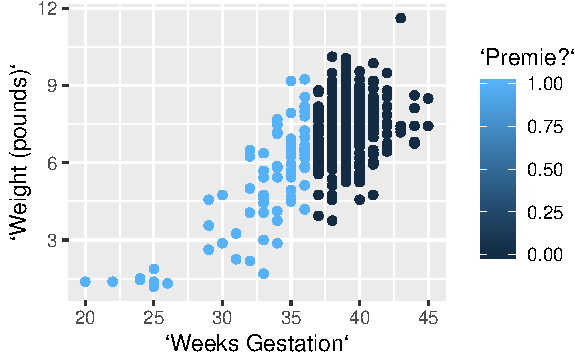
\includegraphics{03-data-summaries_files/figure-latex/unnamed-chunk-24-1}

Better.

With the normal-length pregnancies (red), there seems to be no
relationship between length of pregnancy and birth weight, just a random
variation. But with the premature births, a shorter pregnancy typically
goes with a \emph{lower} birth weight. This would be why the birth
weights for the premature births were more variable.

\begin{enumerate}
\def\labelenumi{(\alph{enumi})}
\setcounter{enumi}{2}
\tightlist
\item
  Do a web search to find the standard (North American) definition of a
  premature birth. Does that correspond to what you saw in the data?
  Cite the website you used, for example by saying ``according to
  \texttt{URL}, ldots'', with \texttt{URL} replaced by the address of
  the website you found.
\end{enumerate}

Solution

The website
\url{http://www.mayoclinic.org/diseases-conditions/premature-birth/basics/definition/con-20020050}
says that ``a premature birth is one that occurs before the start of the
37th week of pregnancy'', which is exactly what we found. (Note that I
am citing the webpage on which I found this, and I even made it into a
link so that you can check it.) The Mayo Clinic is a famous hospital
system with locations in several US states, so I think we can trust what
its website says.

\hypertarget{nenana-alaska}{%
\section{Nenana, Alaska}\label{nenana-alaska}}

Nenana, Alaska, is about 50 miles west of Fairbanks. Every spring, there
is a contest in Nenana. A wooden tripod is placed on the frozen river,
and people try to guess the exact minute when the ice melts enough for
the tripod to fall through the ice. The contest started in 1917 as an
amusement for railway workers, and has taken place every year since.
Now, hundreds of thousands of people enter their guesses on the Internet
and the prize for the winner can be as much as \$300,000.

Because so much money is at stake, and because the exact same tripod is
placed at the exact same spot on the ice every year, the data are
consistent and accurate. The data are in
\href{http://www.utsc.utoronto.ca/~butler/c32/nenana.txt}{link}.

\begin{enumerate}
\def\labelenumi{(\alph{enumi})}
\tightlist
\item
  Read the data into R. Note that the values are separated by
  \emph{tabs} rather than spaces, so you'll need an appropriate
  \texttt{read\_} to read it in.
\end{enumerate}

Solution

These are ``tab-separated values'', so \texttt{read\_tsv} is the thing,
as for the Australian athletes:

\begin{Shaded}
\begin{Highlighting}[]
\NormalTok{myurl =}\StringTok{ "http://www.utsc.utoronto.ca/~butler/c32/nenana.txt"}
\NormalTok{nenana =}\StringTok{ }\KeywordTok{read_tsv}\NormalTok{(myurl)}
\end{Highlighting}
\end{Shaded}

\begin{verbatim}
## Parsed with column specification:
## cols(
##   Year = col_integer(),
##   JulianDate = col_double(),
##   `Date&Time` = col_character()
## )
\end{verbatim}

Use whatever name you like for the data frame. One that is different
from any of the column headers is smart; then it is clear whether you
mean the whole data frame or one of its columns. \texttt{ice} or
\texttt{melt} or anything like that would also be good.

I haven't asked you to display or check the data (that's coming up), but
if you look at it and find that it didn't work, you'll know to come back
and try this part again. R usually gets it right or gives you an error.

If you look at the data, they do appear to be separated by spaces, but
the text version of the date and time \emph{also} have spaces in them,
so things might go astray if you try and read the values in without
recognizing that the actual separator is a tab:

\begin{Shaded}
\begin{Highlighting}[]
\NormalTok{x =}\StringTok{ }\KeywordTok{read_delim}\NormalTok{(myurl, }\StringTok{" "}\NormalTok{)}
\end{Highlighting}
\end{Shaded}

\begin{verbatim}
## Parsed with column specification:
## cols(
##   `Year  JulianDate  Date&Time` = col_character()
## )
\end{verbatim}

\begin{verbatim}
## Warning in rbind(names(probs), probs_f):
## number of columns of result is not a multiple
## of vector length (arg 1)
\end{verbatim}

\begin{verbatim}
## Warning: 87 parsing failures.
## row # A tibble: 5 x 5 col     row col   expected  actual file          expected   <int> <chr> <chr>     <chr>  <chr>         actual 1     1 <NA>  1 columns 5 col~ 'http://www.~ file 2     2 <NA>  1 columns 5 col~ 'http://www.~ row 3     3 <NA>  1 columns 5 col~ 'http://www.~ col 4     4 <NA>  1 columns 5 col~ 'http://www.~ expected 5     5 <NA>  1 columns 5 col~ 'http://www.~
## ... ................. ... ............................................ ........ ............................................ ...... ............................................ .... ............................................ ... ............................................ ... ............................................ ........ ............................................
## See problems(...) for more details.
\end{verbatim}

Ouch! A hint as to what went wrong comes from looking at the read-in
data frame:

\begin{Shaded}
\begin{Highlighting}[]
\NormalTok{x}
\end{Highlighting}
\end{Shaded}

\begin{verbatim}
## # A tibble: 87 x 1
##    `Year\tJulianDate\tDate&Time`
##    <chr>                        
##  1 "1917\t120.4795\tApril"      
##  2 "1918\t131.3983\tMay"        
##  3 "1919\t123.6066\tMay"        
##  4 "1920\t132.4490\tMay"        
##  5 "1921\t131.2795\tMay"        
##  6 "1922\t132.5559\tMay"        
##  7 "1923\t129.0837\tMay"        
##  8 "1924\t132.6323\tMay"        
##  9 "1925\t127.7726\tMay"        
## 10 "1926\t116.6691\tApril"      
## # ... with 77 more rows
\end{verbatim}

Those \texttt{t} symbols mean ``tab character'', which is our hint that
the values were separated by tabs rather than spaces.

More detail (if you can bear to see it) is here:

\begin{Shaded}
\begin{Highlighting}[]
\KeywordTok{problems}\NormalTok{(x)}
\end{Highlighting}
\end{Shaded}

\begin{verbatim}
## # A tibble: 87 x 5
##      row col   expected  actual file        
##    <int> <chr> <chr>     <chr>  <chr>       
##  1     1 <NA>  1 columns 5 col~ 'http://www~
##  2     2 <NA>  1 columns 5 col~ 'http://www~
##  3     3 <NA>  1 columns 5 col~ 'http://www~
##  4     4 <NA>  1 columns 5 col~ 'http://www~
##  5     5 <NA>  1 columns 5 col~ 'http://www~
##  6     6 <NA>  1 columns 5 col~ 'http://www~
##  7     7 <NA>  1 columns 5 col~ 'http://www~
##  8     8 <NA>  1 columns 5 col~ 'http://www~
##  9     9 <NA>  1 columns 5 col~ 'http://www~
## 10    10 <NA>  1 columns 5 col~ 'http://www~
## # ... with 77 more rows
\end{verbatim}

The first line of the data file (with the variable names in it) had no
spaces, only tabs, so \texttt{read\_delim} thinks there is \emph{one}
column with a very long name, but in the actual data, there are
\emph{five} space-separated columns. The text date-times are of the form
``April 30 at 11:30 AM'', which, if you think it's all separated by
spaces, is actually 5 things: April, 30, at and so on. These are the
only things that are separated by spaces, so, from that point of view,
there are five columns.

\begin{enumerate}
\def\labelenumi{(\alph{enumi})}
\setcounter{enumi}{1}
\tightlist
\item
  Find a way of displaying how many rows and columns your data frame
  has, and some of the values. Describe the first and last of the
  variables that you appear to have.
\end{enumerate}

Solution

The easiest is just to display the tibble:

\begin{Shaded}
\begin{Highlighting}[]
\NormalTok{nenana}
\end{Highlighting}
\end{Shaded}

\begin{verbatim}
## # A tibble: 87 x 3
##     Year JulianDate `Date&Time`         
##    <int>      <dbl> <chr>               
##  1  1917       120. April 30 at 11:30 AM
##  2  1918       131. May 11 at 9:33 AM   
##  3  1919       124. May 3 at 2:33 PM    
##  4  1920       132. May 11 at 10:46 AM  
##  5  1921       131. May 11 at 6:42 AM   
##  6  1922       133. May 12 at 1:20 PM   
##  7  1923       129. May 9 at 2:00 AM    
##  8  1924       133. May 11 at 3:10 PM   
##  9  1925       128. May 7 at 6:32 PM    
## 10  1926       117. April 26 at 4:03 PM 
## # ... with 77 more rows
\end{verbatim}

Alternatively, you can take a \texttt{glimpse} of it:

\begin{Shaded}
\begin{Highlighting}[]
\KeywordTok{glimpse}\NormalTok{(nenana)}
\end{Highlighting}
\end{Shaded}

\begin{verbatim}
## Observations: 87
## Variables: 3
## $ Year        <int> 1917, 1918, 1919, 19...
## $ JulianDate  <dbl> 120.4795, 131.3983, ...
## $ `Date&Time` <chr> "April 30 at 11:30 A...
\end{verbatim}

There are 87 years, and 3 columns (variables). The first column is year,
and the last column is the date and time that the tripod fell into the
river, written as a piece of text. I explain the second column in a
moment.

\begin{enumerate}
\def\labelenumi{(\alph{enumi})}
\setcounter{enumi}{2}
\tightlist
\item
  Dates and times are awkward to handle with software. (We see more ways
  later in the course.) The column \texttt{JulianDate} expresses the
  time that the tripod fell through the ice as a fractional number of
  days since December 31. This enables the time (as a fraction of the
  way through the day) to be recorded as well, the whole thing being an
  ordinary number. Make a histogram of the Julian dates. Comment briefly
  on its shape.
\end{enumerate}

Solution

With a \texttt{ggplot} histogram, we need a number of bins first. I can
do Sturges' rule in my head: the next power of 2 up from 87 (our \(n\))
is 128, which is \(2^7\), so the base 2 log of 87 rounds up to 7. That
plus one is 8, so we need 8 bins. For you, any not-insane number of bins
will do, or any not-insane bin width, if you want to go that way:

\begin{Shaded}
\begin{Highlighting}[]
\KeywordTok{ggplot}\NormalTok{(nenana, }\KeywordTok{aes}\NormalTok{(}\DataTypeTok{x =}\NormalTok{ JulianDate)) }\OperatorTok{+}\StringTok{ }\KeywordTok{geom_histogram}\NormalTok{(}\DataTypeTok{bins =} \DecValTok{8}\NormalTok{)}
\end{Highlighting}
\end{Shaded}

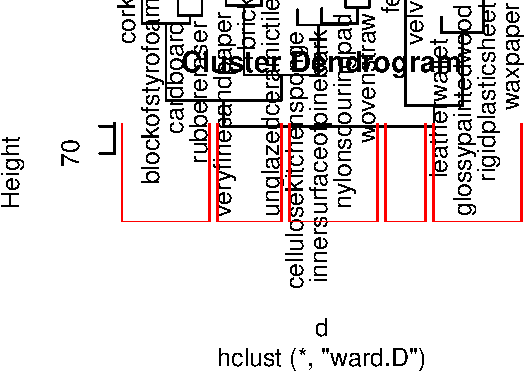
\includegraphics{03-data-summaries_files/figure-latex/unnamed-chunk-31-1}

Note that you need to type \texttt{JulianDate} exactly as it appears,
capital letters and all. R is case-sensitive.

This histogram looks more or less symmetric (and, indeed, normal). I
really don't think you can justify an answer other than ``symmetric''
here. (Or ``approximately normal'': that's good too.) If your histogram
is different, say so. I think that ``hole'' in the middle is not
especially important.

We haven't done normal quantile plots yet, but looking ahead:

\begin{Shaded}
\begin{Highlighting}[]
\KeywordTok{ggplot}\NormalTok{(nenana, }\KeywordTok{aes}\NormalTok{(}\DataTypeTok{sample =}\NormalTok{ JulianDate)) }\OperatorTok{+}\StringTok{ }\KeywordTok{stat_qq}\NormalTok{() }\OperatorTok{+}\StringTok{ }
\StringTok{    }\KeywordTok{stat_qq_line}\NormalTok{()}
\end{Highlighting}
\end{Shaded}

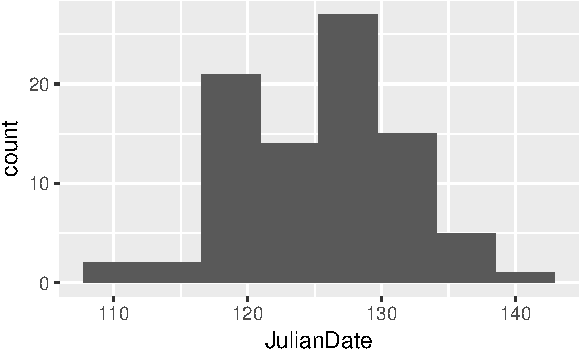
\includegraphics{03-data-summaries_files/figure-latex/unnamed-chunk-32-1}

That hugs the line pretty well, so I would call it close to
normally-distributed. It bulges away from the line because there are
more values just below 120 than you would expect for a normal. This
corresponds to the histogram bar centred just below 120 being taller
than you would have expected.
\marginnote{That is to say, the  principal deviation from normality is not the hole on the histogram, the bar centred around 123 being too short, but that the bar centred just below 120 is too *tall*.}

Extra: looking \emph{way} ahead (to almost the end of the R stuff), this
is how you handle the dates and times:

\begin{Shaded}
\begin{Highlighting}[]
\KeywordTok{library}\NormalTok{(lubridate)}
\end{Highlighting}
\end{Shaded}

\begin{verbatim}
## 
## Attaching package: 'lubridate'
\end{verbatim}

\begin{verbatim}
## The following object is masked from 'package:base':
## 
##     date
\end{verbatim}

\begin{Shaded}
\begin{Highlighting}[]
\NormalTok{nenana }\OperatorTok\StringTok{ }\KeywordTok{mutate}\NormalTok{(}\DataTypeTok{longdt =} \KeywordTok{str_c}\NormalTok{(Year, }\StringTok{" "}\NormalTok{, }\StringTok{`}\DataTypeTok{Date&Time}\StringTok{`}\NormalTok{)) }\OperatorTok\StringTok{ }
\StringTok{    }\KeywordTok{mutate}\NormalTok{(}\DataTypeTok{datetime =} \KeywordTok{ymd_hm}\NormalTok{(longdt, }\DataTypeTok{tz =} \StringTok{"America/Anchorage"}\NormalTok{))}
\end{Highlighting}
\end{Shaded}

\begin{verbatim}
## # A tibble: 87 x 5
##     Year JulianDate `Date&Time` longdt
##    <int>      <dbl> <chr>       <chr> 
##  1  1917       120. April 30 a~ 1917 ~
##  2  1918       131. May 11 at ~ 1918 ~
##  3  1919       124. May 3 at 2~ 1919 ~
##  4  1920       132. May 11 at ~ 1920 ~
##  5  1921       131. May 11 at ~ 1921 ~
##  6  1922       133. May 12 at ~ 1922 ~
##  7  1923       129. May 9 at 2~ 1923 ~
##  8  1924       133. May 11 at ~ 1924 ~
##  9  1925       128. May 7 at 6~ 1925 ~
## 10  1926       117. April 26 a~ 1926 ~
## # ... with 77 more rows, and 1 more
## #   variable: datetime <dttm>
\end{verbatim}

I am not doing any further analysis with these, so just displaying them
is good.

I have to do a preliminary step to get the date-times \emph{with} their
year in one place. \texttt{str\_c} glues pieces of text together: in
this case, the year, a space, and then the rest of the
\texttt{Date\&Time}. I stored this in \texttt{longdt}. The second
\texttt{mutate} is the business end of it: \texttt{ymd\_hm} takes a
piece of text containing a year, month (by name or number), day, hours,
minutes \emph{in that order}, and extracts those things from it, storing
the whole thing as an R date-time. Note that the AM/PM was handled
properly. The benefit of doing that is we can extract anything from the
dates, such as the month or day of week, or take differences between the
dates. Or even check that the Julian dates were calculated correctly
(the \texttt{lubridate} function is called \texttt{yday} for ``day of
year''):

\begin{Shaded}
\begin{Highlighting}[]
\NormalTok{nenana2 <-}\StringTok{ }\NormalTok{nenana }\OperatorTok\StringTok{ }\KeywordTok{mutate}\NormalTok{(}\DataTypeTok{longdt =} \KeywordTok{str_c}\NormalTok{(Year, }
    \StringTok{" "}\NormalTok{, }\StringTok{`}\DataTypeTok{Date&Time}\StringTok{`}\NormalTok{)) }\OperatorTok\StringTok{ }\KeywordTok{mutate}\NormalTok{(}\DataTypeTok{datetime =} \KeywordTok{ymd_hm}\NormalTok{(longdt, }
    \DataTypeTok{tz =} \StringTok{"America/Anchorage"}\NormalTok{)) }\OperatorTok\StringTok{ }\KeywordTok{mutate}\NormalTok{(}\DataTypeTok{jd =} \KeywordTok{yday}\NormalTok{(datetime))}
\NormalTok{nenana2 }\OperatorTok\StringTok{ }\KeywordTok{select}\NormalTok{(JulianDate, jd, datetime)}
\end{Highlighting}
\end{Shaded}

\begin{verbatim}
## # A tibble: 87 x 3
##    JulianDate    jd datetime           
##         <dbl> <dbl> <dttm>             
##  1       120.   120 1917-04-30 11:30:00
##  2       131.   131 1918-05-11 09:33:00
##  3       124.   123 1919-05-03 14:33:00
##  4       132.   132 1920-05-11 10:46:00
##  5       131.   131 1921-05-11 06:42:00
##  6       133.   132 1922-05-12 13:20:00
##  7       129.   129 1923-05-09 02:00:00
##  8       133.   132 1924-05-11 15:10:00
##  9       128.   127 1925-05-07 18:32:00
## 10       117.   116 1926-04-26 16:03:00
## # ... with 77 more rows
\end{verbatim}

Hmm, some of those are off by one. What do the off-by-one ones have in
common? Let's look at more of them. \texttt{round} rounds off to the
nearest integer (since these are actually decimal numbers):

\begin{Shaded}
\begin{Highlighting}[]
\NormalTok{nenana2 }\OperatorTok\StringTok{ }\KeywordTok{filter}\NormalTok{(}\KeywordTok{round}\NormalTok{(JulianDate) }\OperatorTok{!=}\StringTok{ }\KeywordTok{round}\NormalTok{(jd)) }\OperatorTok\StringTok{ }
\StringTok{    }\KeywordTok{select}\NormalTok{(JulianDate, jd, datetime)}
\end{Highlighting}
\end{Shaded}

\begin{verbatim}
## # A tibble: 61 x 3
##    JulianDate    jd datetime           
##         <dbl> <dbl> <dttm>             
##  1       124.   123 1919-05-03 14:33:00
##  2       133.   132 1922-05-12 13:20:00
##  3       133.   132 1924-05-11 15:10:00
##  4       128.   127 1925-05-07 18:32:00
##  5       117.   116 1926-04-26 16:03:00
##  6       128.   127 1928-05-06 16:25:00
##  7       126.   125 1929-05-05 15:41:00
##  8       129.   128 1930-05-08 19:03:00
##  9       129.   128 1933-05-08 19:30:00
## 10       121.   120 1934-04-30 14:07:00
## # ... with 51 more rows
\end{verbatim}

The ones shown here are all \emph{after noon}, and the Julian date in
the data file appears as one more than the one calculated by
\texttt{lubridate}. What has actually happened is a quirk of how tibbles
are displayed: they show 3 significant digits, \emph{rounded}. The
Julian dates given by \texttt{yday} are the whole-number part, so the
ones in the data value are that plus more than 0.5, which will round
\emph{up}. The first line of code below displays 6 significant digits
rather than only three:

\begin{Shaded}
\begin{Highlighting}[]
\KeywordTok{options}\NormalTok{(}\DataTypeTok{pillar.sigfig =} \DecValTok{6}\NormalTok{)}
\NormalTok{nenana2 }\OperatorTok\StringTok{ }\KeywordTok{filter}\NormalTok{(}\KeywordTok{round}\NormalTok{(JulianDate) }\OperatorTok{!=}\StringTok{ }\KeywordTok{round}\NormalTok{(jd)) }\OperatorTok\StringTok{ }
\StringTok{    }\KeywordTok{select}\NormalTok{(JulianDate, jd, datetime)}
\end{Highlighting}
\end{Shaded}

\begin{verbatim}
## # A tibble: 61 x 3
##    JulianDate    jd datetime           
##         <dbl> <dbl> <dttm>             
##  1    123.607   123 1919-05-03 14:33:00
##  2    132.556   132 1922-05-12 13:20:00
##  3    132.632   132 1924-05-11 15:10:00
##  4    127.773   127 1925-05-07 18:32:00
##  5    116.669   116 1926-04-26 16:03:00
##  6    127.684   127 1928-05-06 16:25:00
##  7    125.654   125 1929-05-05 15:41:00
##  8    128.794   128 1930-05-08 19:03:00
##  9    128.813   128 1933-05-08 19:30:00
## 10    120.588   120 1934-04-30 14:07:00
## # ... with 51 more rows
\end{verbatim}

Displaying more decimals shows that I was right: \texttt{jd} is (to this
accuracy) a whole number, but \texttt{JulianDate} is a decimal with
fractional part greater than 0.50.

Now I have to turn the extra signficant digits off:

\begin{Shaded}
\begin{Highlighting}[]
\KeywordTok{options}\NormalTok{(}\DataTypeTok{pillar.sigfig =} \DecValTok{3}\NormalTok{)}
\end{Highlighting}
\end{Shaded}

\begin{enumerate}
\def\labelenumi{(\alph{enumi})}
\setcounter{enumi}{3}
\tightlist
\item
  Plot \texttt{JulianDate} against \texttt{Year} on a scatterplot. What
  recent trends, if any, do you see? Comment briefly.
\end{enumerate}

Solution

\texttt{geom\_point}:

\begin{Shaded}
\begin{Highlighting}[]
\KeywordTok{ggplot}\NormalTok{(nenana, }\KeywordTok{aes}\NormalTok{(}\DataTypeTok{x =}\NormalTok{ Year, }\DataTypeTok{y =}\NormalTok{ JulianDate)) }\OperatorTok{+}\StringTok{ }
\StringTok{    }\KeywordTok{geom_point}\NormalTok{()}
\end{Highlighting}
\end{Shaded}

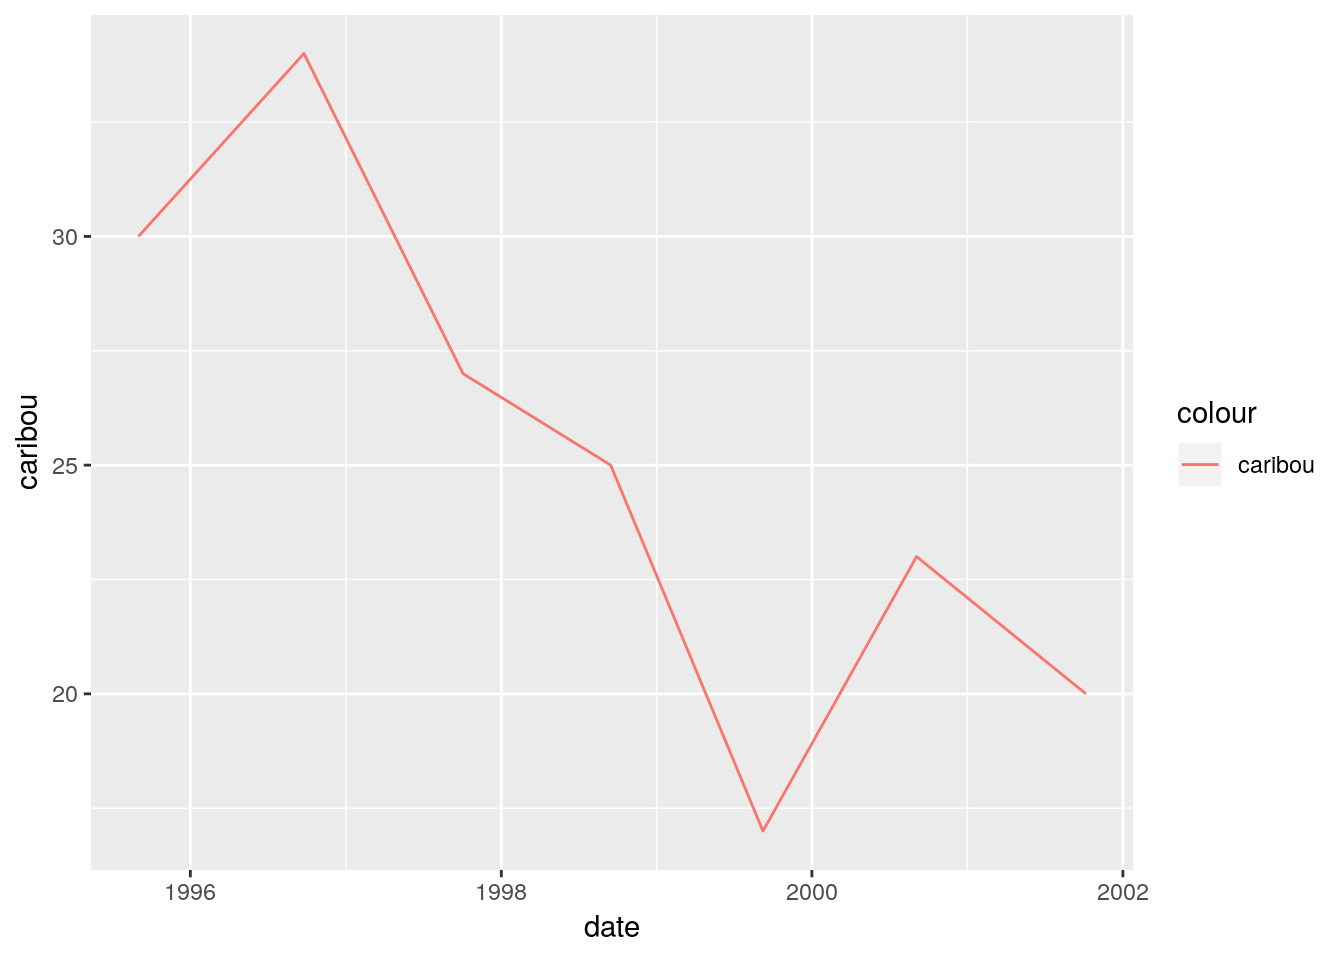
\includegraphics{03-data-summaries_files/figure-latex/unnamed-chunk-38-1}

This is actually a small-but-real downward trend, especially since about
1960, but the large amount of variability makes it hard to see, so I'm
good with either ``no trend'' or ``weak downward trend'' or anything
roughly like that. There is definitely not much trend before 1960, but
most of the really early break-ups (less than about 118) have been since
about 1990.

You can even add to the \texttt{ggplot}, by putting a smooth trend on
it:

\begin{Shaded}
\begin{Highlighting}[]
\KeywordTok{ggplot}\NormalTok{(nenana, }\KeywordTok{aes}\NormalTok{(}\DataTypeTok{x =}\NormalTok{ Year, }\DataTypeTok{y =}\NormalTok{ JulianDate)) }\OperatorTok{+}\StringTok{ }
\StringTok{    }\KeywordTok{geom_point}\NormalTok{() }\OperatorTok{+}\StringTok{ }\KeywordTok{geom_smooth}\NormalTok{()}
\end{Highlighting}
\end{Shaded}

\begin{verbatim}
## `geom_smooth()` using method = 'loess' and formula 'y ~ x'
\end{verbatim}

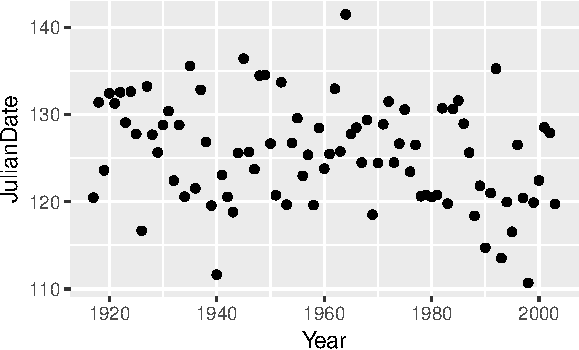
\includegraphics{03-data-summaries_files/figure-latex/unnamed-chunk-39-1}

This is R's version of a trend that is not constrained to be linear (so
that it ``lets the data speak for itself'').

Now there is something obvious to see: after about 1960, there is a
clear downward trend: the ice is breaking up earlier on average every
year. Even though there is a lot of variability, the overall trend,
viewed this way, is clear.

What does this mean, in practice? This notion of the ice melting earlier
than it used to is consistent all over the Arctic, and is one more
indication of climate change. Precisely, it is an indication that
climate change is happening, but we would have to delve further to make
any statements about the \emph{cause} of that climate change.

\hypertarget{computerized-accounting}{%
\section{Computerized accounting}\label{computerized-accounting}}

Beginning accounting students need to learn to learn to audit in a
computerized environment. A sample of beginning accounting students took
each of two tests: the Computer Attitude Scale (CAS) and the Computer
Anxiety Rating Scale (CARS). A higher score in each indicates greater
anxiety around computers. The test scores are scaled to be between 0 and
5. Also noted was each student's gender. The data are in
\url{http://www.utsc.utoronto.ca/~butler/c32/compatt.txt}. The data
values are separated by spaces.

\begin{enumerate}
\def\labelenumi{(\alph{enumi})}
\tightlist
\item
  Read the data into R. Do you have what you expected? Explain briefly.
\end{enumerate}

Solution

Read in and display the data. This, I think, is the easiest way.

\begin{Shaded}
\begin{Highlighting}[]
\NormalTok{url =}\StringTok{ "http://www.utsc.utoronto.ca/~butler/c32/compatt.txt"}
\NormalTok{anxiety =}\StringTok{ }\KeywordTok{read_delim}\NormalTok{(url, }\StringTok{" "}\NormalTok{)}
\end{Highlighting}
\end{Shaded}

\begin{verbatim}
## Parsed with column specification:
## cols(
##   gender = col_character(),
##   CAS = col_double(),
##   CARS = col_double()
## )
\end{verbatim}

\begin{Shaded}
\begin{Highlighting}[]
\NormalTok{anxiety}
\end{Highlighting}
\end{Shaded}

\begin{verbatim}
## # A tibble: 35 x 3
##    gender   CAS  CARS
##    <chr>  <dbl> <dbl>
##  1 female  2.85  2.9 
##  2 male    2.6   2.32
##  3 female  2.2   1   
##  4 male    2.65  2.58
##  5 male    2.6   2.58
##  6 male    3.2   3.05
##  7 male    3.65  3.74
##  8 female  2.55  1.9 
##  9 male    3.15  3.32
## 10 male    2.8   2.74
## # ... with 25 more rows
\end{verbatim}

There is a total of 35 students with a CAS score, a CARS score and a
gender recorded for each. This is in line with what I was expecting.
(You can also note that the genders appear to be a mixture of males and
females.)

\begin{enumerate}
\def\labelenumi{(\alph{enumi})}
\setcounter{enumi}{1}
\tightlist
\item
  How many males and females were there in the sample?
\end{enumerate}

Solution

Most easily \texttt{count}:

\begin{Shaded}
\begin{Highlighting}[]
\NormalTok{anxiety }\OperatorTok\StringTok{ }\KeywordTok{count}\NormalTok{(gender)}
\end{Highlighting}
\end{Shaded}

\begin{verbatim}
## # A tibble: 2 x 2
##   gender     n
##   <chr>  <int>
## 1 female    15
## 2 male      20
\end{verbatim}

This also works (and is therefore good):

\begin{Shaded}
\begin{Highlighting}[]
\NormalTok{anxiety }\OperatorTok\StringTok{ }\KeywordTok{group_by}\NormalTok{(gender) }\OperatorTok\StringTok{ }\KeywordTok{summarize}\NormalTok{(}\DataTypeTok{count =} \KeywordTok{n}\NormalTok{())}
\end{Highlighting}
\end{Shaded}

\begin{verbatim}
## # A tibble: 2 x 2
##   gender count
##   <chr>  <int>
## 1 female    15
## 2 male      20
\end{verbatim}

I want you to use R to do the counting (that is, don't just list out the
whole data set with \texttt{print(n=Inf)} and count the males and
females yourself). This is because you might have thousands of data
values and you need to learn how to get R (or, later, SAS) to count them
for you.

15 females and 20 males, \emph{which you should say}. I made a point of
\emph{not} saying that it is enough to get the output with the answers
on it, so you need to tell me what the answer is.

\begin{enumerate}
\def\labelenumi{(\alph{enumi})}
\setcounter{enumi}{2}
\tightlist
\item
  Do the CAS scores tend to be higher for females or for males? Draw a
  suitable graph to help you decide, and come to a conclusion.
\end{enumerate}

Solution

Gender is categorical and CAS score is quantitative, so a boxplot would
appear to be the thing:

\begin{Shaded}
\begin{Highlighting}[]
\KeywordTok{ggplot}\NormalTok{(anxiety, }\KeywordTok{aes}\NormalTok{(}\DataTypeTok{x =}\NormalTok{ gender, }\DataTypeTok{y =}\NormalTok{ CAS)) }\OperatorTok{+}\StringTok{ }\KeywordTok{geom_boxplot}\NormalTok{()}
\end{Highlighting}
\end{Shaded}

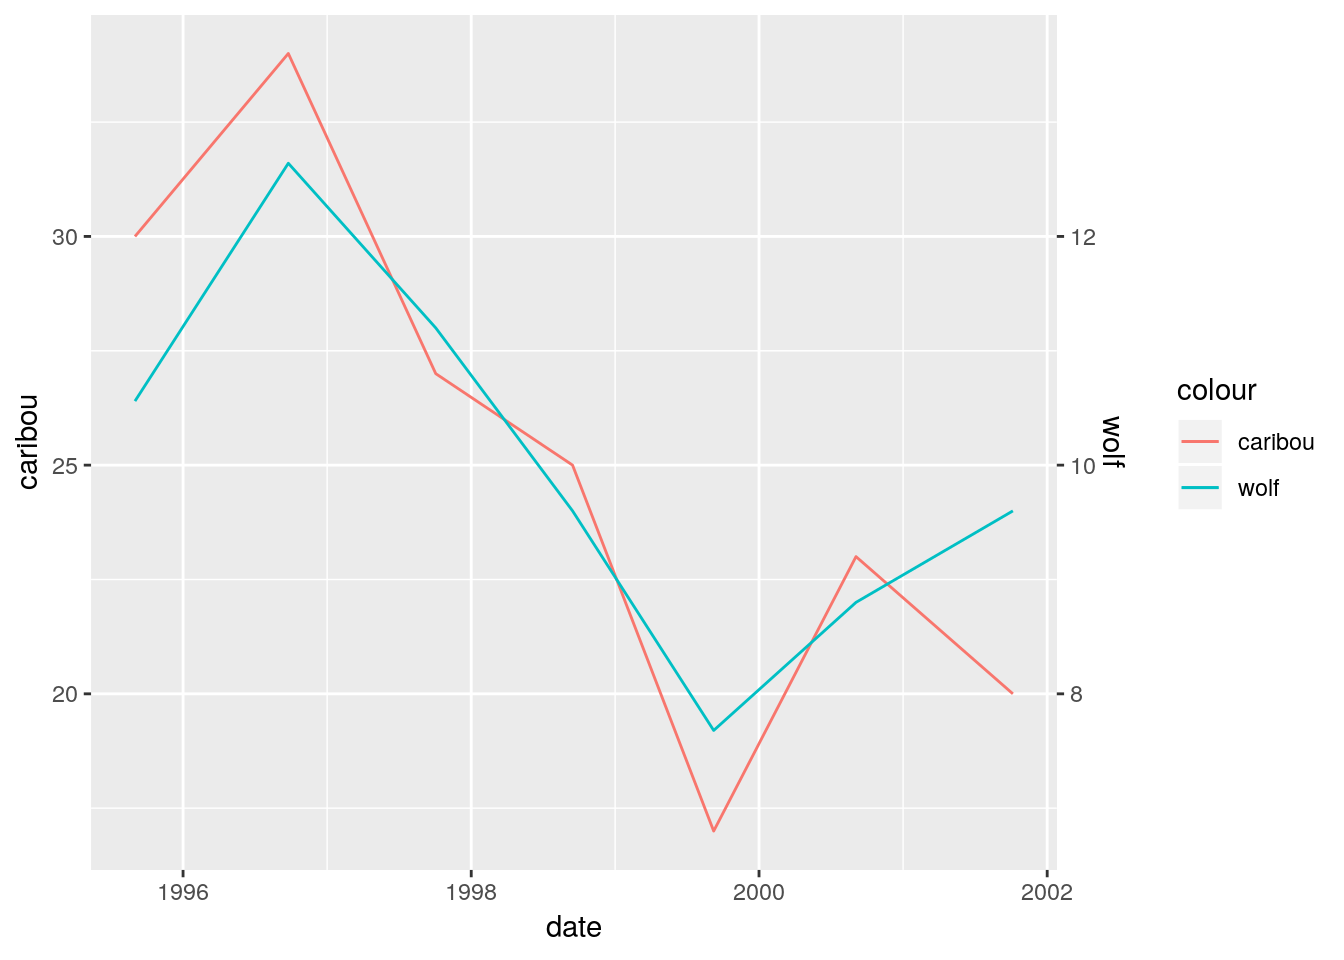
\includegraphics{03-data-summaries_files/figure-latex/unnamed-chunk-43-1}

The median for males is slightly higher, so male accountants are more
anxious around computers than female accountants are.

If you wish, side-by-side (or, better, above-and-below) histograms would
also work:

\begin{Shaded}
\begin{Highlighting}[]
\KeywordTok{ggplot}\NormalTok{(anxiety, }\KeywordTok{aes}\NormalTok{(}\DataTypeTok{x =}\NormalTok{ CAS)) }\OperatorTok{+}\StringTok{ }\KeywordTok{geom_histogram}\NormalTok{(}\DataTypeTok{bins =} \DecValTok{6}\NormalTok{) }\OperatorTok{+}\StringTok{ }
\StringTok{    }\KeywordTok{facet_wrap}\NormalTok{(}\OperatorTok{~}\NormalTok{gender, }\DataTypeTok{ncol =} \DecValTok{1}\NormalTok{)}
\end{Highlighting}
\end{Shaded}

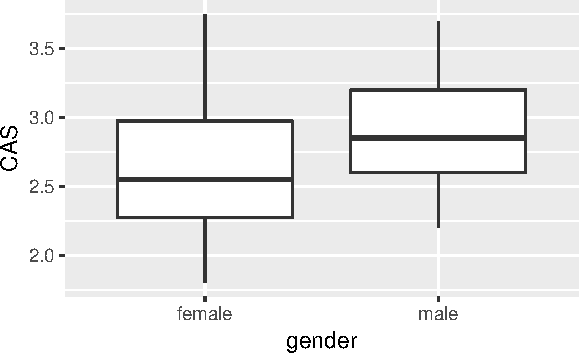
\includegraphics{03-data-summaries_files/figure-latex/unnamed-chunk-44-1}

If you go this way, you have to make a call about where the centres of
the histograms are. I guess the male one is slightly further to the
right, but it's not so easy to tell. (Make a call.)

\begin{enumerate}
\def\labelenumi{(\alph{enumi})}
\setcounter{enumi}{3}
\tightlist
\item
  Find the median CAS scores for each gender. Does this support what you
  saw on your plot? Explain briefly.
\end{enumerate}

Solution

Group-by and summarize:

\begin{Shaded}
\begin{Highlighting}[]
\NormalTok{anxiety }\OperatorTok\StringTok{ }\KeywordTok{group_by}\NormalTok{(gender) }\OperatorTok\StringTok{ }\KeywordTok{summarize}\NormalTok{(}\DataTypeTok{med =} \KeywordTok{median}\NormalTok{(CAS))}
\end{Highlighting}
\end{Shaded}

\begin{verbatim}
## # A tibble: 2 x 2
##   gender   med
##   <chr>  <dbl>
## 1 female  2.55
## 2 male    2.85
\end{verbatim}

The median is a bit higher for males, which is what I got on my boxplot
(and is apparently the same thing as is on the histograms, but it's
harder to be sure there).

\begin{enumerate}
\def\labelenumi{(\alph{enumi})}
\setcounter{enumi}{4}
\tightlist
\item
  Find the mean and standard deviation of both CAS and CARS scores (for
  all the students combined, ie.~not separated by gender) \emph{without}
  naming those columns explicitly.
\end{enumerate}

Solution

Without naming them explicitly means using some other way to pick them
out of the data frame, either \texttt{summarize\textbackslash{}\_if} or
\texttt{summarize\textbackslash{}\_at}. To do it the first way, ask what
these two columns have in common: they are the only two numeric
(quantitative) columns:

\begin{Shaded}
\begin{Highlighting}[]
\NormalTok{anxiety }\OperatorTok\StringTok{ }\KeywordTok{summarize_if}\NormalTok{(is.numeric, }\KeywordTok{funs}\NormalTok{(mean, }
\NormalTok{    sd))}
\end{Highlighting}
\end{Shaded}

\begin{verbatim}
## # A tibble: 1 x 4
##   CAS_mean CARS_mean CAS_sd CARS_sd
##      <dbl>     <dbl>  <dbl>   <dbl>
## 1     2.82      2.77  0.484   0.671
\end{verbatim}

Or the second way, asking yourself what the \emph{names} of those
columns have in common: they start with C and the gender column doesn't:

\begin{Shaded}
\begin{Highlighting}[]
\NormalTok{anxiety }\OperatorTok\StringTok{ }\KeywordTok{summarize_at}\NormalTok{(}\KeywordTok{vars}\NormalTok{(}\KeywordTok{starts_with}\NormalTok{(}\StringTok{"C"}\NormalTok{)), }
    \KeywordTok{funs}\NormalTok{(mean, sd))}
\end{Highlighting}
\end{Shaded}

\begin{verbatim}
## # A tibble: 1 x 4
##   CAS_mean CARS_mean CAS_sd CARS_sd
##      <dbl>     <dbl>  <dbl>   <dbl>
## 1     2.82      2.77  0.484   0.671
\end{verbatim}

Either of these is good, or anything equivalent (like noting that the
two anxiety scales both \texttt{ends\textbackslash{}\_with} S):

\begin{Shaded}
\begin{Highlighting}[]
\NormalTok{anxiety }\OperatorTok\StringTok{ }\KeywordTok{summarize_at}\NormalTok{(}\KeywordTok{vars}\NormalTok{(}\KeywordTok{ends_with}\NormalTok{(}\StringTok{"S"}\NormalTok{)), }
    \KeywordTok{funs}\NormalTok{(mean, sd))}
\end{Highlighting}
\end{Shaded}

\begin{verbatim}
## # A tibble: 1 x 4
##   CAS_mean CARS_mean CAS_sd CARS_sd
##      <dbl>     <dbl>  <dbl>   <dbl>
## 1     2.82      2.77  0.484   0.671
\end{verbatim}

Because I didn't say otherwise, you should tell me what the means and
SDs are, rounding off suitably: the CAS scores have mean 2.82 and SD
0.48, and the CARS scores have mean 2.77 and SD 0.67.

Yet another way to do it is to select the columns you want first (which
you can do by number so as not to name them), and then find the mean and
SD of all of them. This uses two tools that we haven't seen yet:

\begin{Shaded}
\begin{Highlighting}[]
\NormalTok{anxiety }\OperatorTok\StringTok{ }\KeywordTok{select}\NormalTok{(}\DecValTok{2}\OperatorTok{:}\DecValTok{3}\NormalTok{) }\OperatorTok\StringTok{ }\KeywordTok{summarize_all}\NormalTok{(}\KeywordTok{funs}\NormalTok{(mean, }
\NormalTok{    sd))}
\end{Highlighting}
\end{Shaded}

\begin{verbatim}
## # A tibble: 1 x 4
##   CAS_mean CARS_mean CAS_sd CARS_sd
##      <dbl>     <dbl>  <dbl>   <dbl>
## 1     2.82      2.77  0.484   0.671
\end{verbatim}

This doesn't work:

\begin{Shaded}
\begin{Highlighting}[]
\KeywordTok{summary}\NormalTok{(anxiety)}
\end{Highlighting}
\end{Shaded}

\begin{verbatim}
##     gender               CAS       
##  Length:35          Min.   :1.800  
##  Class :character   1st Qu.:2.575  
##  Mode  :character   Median :2.800  
##                     Mean   :2.816  
##                     3rd Qu.:3.150  
##                     Max.   :3.750  
##       CARS      
##  Min.   :1.000  
##  1st Qu.:2.445  
##  Median :2.790  
##  Mean   :2.771  
##  3rd Qu.:3.290  
##  Max.   :4.000
\end{verbatim}

because, although it gets the means, it does not get the standard
deviations. (I added the SD to the original question to make you find a
way other than this.)

In summary, find a way to get those answers without naming those columns
in your code, and I'm good.

In case you were wondering about how to do this separately by gender,
well, put the \texttt{group\textbackslash{}\_by} in like you did before:

\begin{Shaded}
\begin{Highlighting}[]
\NormalTok{anxiety }\OperatorTok\StringTok{ }\KeywordTok{group_by}\NormalTok{(gender) }\OperatorTok\StringTok{ }\KeywordTok{summarize_if}\NormalTok{(is.numeric, }
    \KeywordTok{funs}\NormalTok{(mean, sd))}
\end{Highlighting}
\end{Shaded}

\begin{verbatim}
## # A tibble: 2 x 5
##   gender CAS_mean CARS_mean CAS_sd CARS_sd
##   <chr>     <dbl>     <dbl>  <dbl>   <dbl>
## 1 female     2.64      2.51  0.554   0.773
## 2 male       2.94      2.96  0.390   0.525
\end{verbatim}

or

\begin{Shaded}
\begin{Highlighting}[]
\NormalTok{anxiety }\OperatorTok\StringTok{ }\KeywordTok{group_by}\NormalTok{(gender) }\OperatorTok\StringTok{ }\KeywordTok{summarize_at}\NormalTok{(}\KeywordTok{vars}\NormalTok{(}\KeywordTok{starts_with}\NormalTok{(}\StringTok{"C"}\NormalTok{)), }
    \KeywordTok{funs}\NormalTok{(mean, sd))}
\end{Highlighting}
\end{Shaded}

\begin{verbatim}
## # A tibble: 2 x 5
##   gender CAS_mean CARS_mean CAS_sd CARS_sd
##   <chr>     <dbl>     <dbl>  <dbl>   <dbl>
## 1 female     2.64      2.51  0.554   0.773
## 2 male       2.94      2.96  0.390   0.525
\end{verbatim}

The male means are slightly higher on both tests, but the male standard
deviations are a little smaller. You might be wondering whether the test
scores are related. They are both quantitative, so the obvious way to
find out is a scatterplot:

\begin{Shaded}
\begin{Highlighting}[]
\KeywordTok{ggplot}\NormalTok{(anxiety, }\KeywordTok{aes}\NormalTok{(}\DataTypeTok{x =}\NormalTok{ CAS, }\DataTypeTok{y =}\NormalTok{ CARS)) }\OperatorTok{+}\StringTok{ }\KeywordTok{geom_point}\NormalTok{()}
\end{Highlighting}
\end{Shaded}

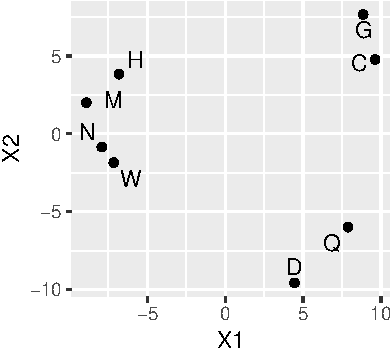
\includegraphics{03-data-summaries_files/figure-latex/unnamed-chunk-53-1}

The two variables can be on either axis, since there is no obvious
response or explanatory variable. A higher score on one scale goes with
a higher score on the other, suggesting that the two scales are
measuring the same thing.

This plot mixes up the males and females, so you might like to
distinguish them, which goes like this:

\begin{Shaded}
\begin{Highlighting}[]
\KeywordTok{ggplot}\NormalTok{(anxiety, }\KeywordTok{aes}\NormalTok{(}\DataTypeTok{x =}\NormalTok{ CAS, }\DataTypeTok{y =}\NormalTok{ CARS, }\DataTypeTok{colour =}\NormalTok{ gender)) }\OperatorTok{+}\StringTok{ }
\StringTok{    }\KeywordTok{geom_point}\NormalTok{()}
\end{Highlighting}
\end{Shaded}

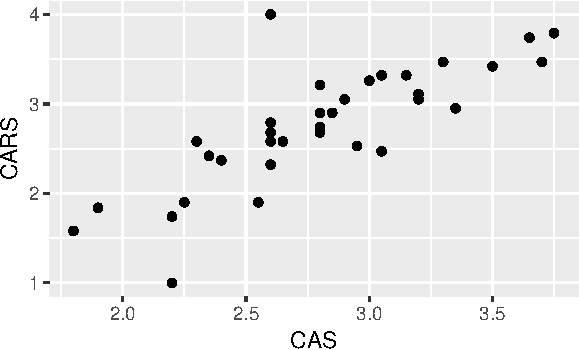
\includegraphics{03-data-summaries_files/figure-latex/unnamed-chunk-54-1}

There is a slight (but only slight) tendency for the males to be up and
to the right, and for the females to be down and to the left. This is
about what you would expect, given that the male means are slightly
bigger on both scores, but the difference in means is not that big
compared to the SD.

\hypertarget{one-sample-inference}{%
\chapter{One-sample inference}\label{one-sample-inference}}

\begin{Shaded}
\begin{Highlighting}[]
\KeywordTok{library}\NormalTok{(tidyverse)}
\end{Highlighting}
\end{Shaded}

\begin{verbatim}
## -- Attaching packages ---- tidyverse 1.2.1 --
\end{verbatim}

\begin{verbatim}
## v ggplot2 3.0.0     v purrr   0.2.5
## v tibble  1.4.2     v dplyr   0.7.6
## v tidyr   0.8.1     v stringr 1.3.1
## v readr   1.1.1     v forcats 0.3.0
\end{verbatim}

\begin{verbatim}
## -- Conflicts ------- tidyverse_conflicts() --
## x dplyr::filter() masks stats::filter()
## x dplyr::lag()    masks stats::lag()
\end{verbatim}

\hypertarget{hunter-gatherers-in-australia}{%
\section{Hunter-gatherers in
Australia}\label{hunter-gatherers-in-australia}}

A hunter-gatherer society is one where people get their food by hunting,
fishing or foraging rather than by agriculture or by raising animals.
Such societies tend to move from place to place. Anthropologists have
studied hunter-gatherer societies in forest ecosystems across the world.
The average population density of these societies is 7.38 people per 100
km\(^2\). Hunter-gatherer societies on different continents might have
different population densities, possibly because of large-scale
ecological constraints (such as resource availability), or because of
other factors, possibly social and/or historic, determining population
density.

Some hunter-gatherer societies in Australia were studied, and the
population density per 100 km\(^2\) recorded for each. The data are in
\url{http://www.utsc.utoronto.ca/~butler/c32/hg.txt}.

\begin{enumerate}
\def\labelenumi{(\alph{enumi})}
\tightlist
\item
  Read the data into R. Do you have the correct variables? How many
  hunter-gatherer societies in Australia were studied? Explain briefly.
\end{enumerate}

Solution

The data values are separated by (single) spaces, so
\texttt{read\_delim} is the thing:

\begin{Shaded}
\begin{Highlighting}[]
\NormalTok{url =}\StringTok{ "http://www.utsc.utoronto.ca/~butler/c32/hg.txt"}
\NormalTok{societies =}\StringTok{ }\KeywordTok{read_delim}\NormalTok{(url, }\StringTok{" "}\NormalTok{)}
\end{Highlighting}
\end{Shaded}

\begin{verbatim}
## Parsed with column specification:
## cols(
##   name = col_character(),
##   density = col_double()
## )
\end{verbatim}

I like to put the URL in a variable first, because if I don't, the
\texttt{read\_delim} line can be rather long. But if you want to do it
in one step, that's fine, as long as it's clear that you are doing the
right thing.

Let's look at the data frame:

\begin{Shaded}
\begin{Highlighting}[]
\NormalTok{societies}
\end{Highlighting}
\end{Shaded}

\begin{verbatim}
## # A tibble: 13 x 2
##    name       density
##    <chr>        <dbl>
##  1 jeidji       17   
##  2 kuku         50   
##  3 mamu         45   
##  4 ngatjan      59.8 
##  5 undanbi      21.7 
##  6 jinibarra    16   
##  7 ualaria       9   
##  8 barkindji    15.4 
##  9 wongaibon     5.12
## 10 jaralde      40   
## 11 tjapwurong   35   
## 12 tasmanians   13.4 
## 13 badjalang    13.4
\end{verbatim}

I have the name of each society and its population density, as promised
(so that is correct). There were 13 societies that were studied. For me,
they were all displayed. For you, you'll probably see only the first
ten, and you'll have to click Next to see the last three.

\begin{enumerate}
\def\labelenumi{(\alph{enumi})}
\setcounter{enumi}{1}
\tightlist
\item
  The question of interest is whether these Australian hunter-gatherer
  societies are like the rest of the world in terms of mean population
  density. State suitable null and alternative hypotheses. \emph{Define
  any symbols you use}: that is, if you use a symbol, you also have to
  say what it means.
\end{enumerate}

Solution

The mean for the world as a whole (``average'', as stated earlier) is
7.38. Let \(\mu\) denote the population mean for Australia (of which
these societies are a sample). Then our hypotheses are:
\[ H_0: \mu=7.38\] and \[ H_a: \mu \ne 7.38.\] There is no reason for a
one-sided alternative here, since all we are interested in is whether
Australia is different from the rest of the world. \emph{Expect to lose
a point} if you use the symbol \(\mu\) without saying what it means.

\begin{enumerate}
\def\labelenumi{(\alph{enumi})}
\setcounter{enumi}{2}
\tightlist
\item
  Test your hypotheses using a suitable test. What do you conclude, in
  the context of the data?
\end{enumerate}

Solution

A \(t\)-test, since we are testing a mean:

\begin{Shaded}
\begin{Highlighting}[]
\KeywordTok{t.test}\NormalTok{(societies}\OperatorTok{$}\NormalTok{density, }\DataTypeTok{mu =} \FloatTok{7.38}\NormalTok{)}
\end{Highlighting}
\end{Shaded}

\begin{verbatim}
## 
##  One Sample t-test
## 
## data:  societies$density
## t = 3.8627, df = 12, p-value = 0.002257
## alternative hypothesis: true mean is not equal to 7.38
## 95 percent confidence interval:
##  15.59244 36.84449
## sample estimates:
## mean of x 
##  26.21846
\end{verbatim}

The P-value is 0.0023, less than the usual \(\alpha\) of 0.05, so we
\emph{reject} the null hypothesis and conclude that the mean population
density is not equal to 7.38. That is to say, Australia is different
from the rest of the world in this sense.

As you know, ``reject the null hypothesis'' is only part of the answer,
so gets only part of the marks.

\begin{enumerate}
\def\labelenumi{(\alph{enumi})}
\setcounter{enumi}{3}
\tightlist
\item
  Do you have any doubts about the validity of your test? Explain
  briefly, using a suitable graph to support your explanation.
\end{enumerate}

Solution

The assumption behind the \(t\)-test is that the data are approximately
normal. We can assess that in several ways, but the simplest (which is
perfectly acceptable at this point) is a histogram. You'll need to pick
a suitable number of bins. This one comes from Sturges' rule:

\begin{Shaded}
\begin{Highlighting}[]
\KeywordTok{ggplot}\NormalTok{(societies, }\KeywordTok{aes}\NormalTok{(}\DataTypeTok{x =}\NormalTok{ density)) }\OperatorTok{+}\StringTok{ }\KeywordTok{geom_histogram}\NormalTok{(}\DataTypeTok{bins =} \DecValTok{5}\NormalTok{)}
\end{Highlighting}
\end{Shaded}

\includegraphics{04-one-sample-inference_files/figure-latex/unnamed-chunk-8-1}
Your conclusion might depend on how many bins you chose for your
histogram. Here's 8 bins (which is really too many with only 13
observations, but it actually shows the shape well):

\begin{Shaded}
\begin{Highlighting}[]
\KeywordTok{ggplot}\NormalTok{(societies, }\KeywordTok{aes}\NormalTok{(}\DataTypeTok{x =}\NormalTok{ density)) }\OperatorTok{+}\StringTok{ }\KeywordTok{geom_histogram}\NormalTok{(}\DataTypeTok{bins =} \DecValTok{8}\NormalTok{)}
\end{Highlighting}
\end{Shaded}

\includegraphics{04-one-sample-inference_files/figure-latex/unnamed-chunk-9-1}

or you can get a number of bins from one of the built-in functions, such
as:

\begin{Shaded}
\begin{Highlighting}[]
\NormalTok{mybins =}\StringTok{ }\KeywordTok{nclass.FD}\NormalTok{(societies}\OperatorTok{$}\NormalTok{density)}
\NormalTok{mybins}
\end{Highlighting}
\end{Shaded}

\begin{verbatim}
## [1] 3
\end{verbatim}

This one is small. The interquartile range is large and \(n\) is small,
so the binwidth will be large and therefore the number of bins will be
small.

Other choices: a one-group boxplot:

\begin{Shaded}
\begin{Highlighting}[]
\KeywordTok{ggplot}\NormalTok{(societies, }\KeywordTok{aes}\NormalTok{(}\DataTypeTok{x =} \DecValTok{1}\NormalTok{, }\DataTypeTok{y =}\NormalTok{ density)) }\OperatorTok{+}\StringTok{ }\KeywordTok{geom_boxplot}\NormalTok{()}
\end{Highlighting}
\end{Shaded}

\includegraphics{04-one-sample-inference_files/figure-latex/unnamed-chunk-11-1}

This isn't the best for assessing normality as such, but it will tell
you about lack of symmetry and outliers, which are the most important
threats to the \(t\)-test, so it's fine here. Or, a normal quantile
plot:

\begin{Shaded}
\begin{Highlighting}[]
\KeywordTok{ggplot}\NormalTok{(societies, }\KeywordTok{aes}\NormalTok{(}\DataTypeTok{sample =}\NormalTok{ density)) }\OperatorTok{+}\StringTok{ }\KeywordTok{stat_qq}\NormalTok{() }\OperatorTok{+}\StringTok{ }
\StringTok{    }\KeywordTok{stat_qq_line}\NormalTok{()}
\end{Highlighting}
\end{Shaded}

\includegraphics{04-one-sample-inference_files/figure-latex/unnamed-chunk-12-1}

This is actually the best way to assess normality, but I'm not expecting
you to use this plot here, because we may not have gotten to it in class
yet. (If you have read ahead and successfully use the plot, it's fine.)

After you have drawn your chosen plot (you need \emph{one} plot), you
need to say something about normality and thus whether you have any
doubts about the validity of your \(t\)-test. This will depend on the
graph you drew: if you think your graph is symmetric and outlier-free,
you should have no doubts about your \(t\)-test; if you think it has
something wrong with it, you should say what it is and express your
doubts. My guess is that you will think this distribution is skewed to
the right. Most of my plots are saying that.
\marginnote{The normal  quantile plot is rather interesting: it says that the uppermost  values are approximately normal, but the *smallest* eight or so  values are too bunched up to be normal. That is, normality fails not  because of the long tail on the right, but the bunching on the  left. Still right-skewed, though.}

On the website where I got these data, they were using the data as an
example for another test, precisely \emph{because} they thought the
distribution was right-skewed. Later on, we'll learn about the sign test
for the median, which I think is actually a better test here.

\hypertarget{length-of-gestation-in-north-carolina}{%
\section{Length of gestation in North
Carolina}\label{length-of-gestation-in-north-carolina}}

The data in file
\href{http://www.utsc.utoronto.ca/~butler/c32/ncbirths.csv}{link} are
about 500 randomly chosen births of babies in North Carolina. There is a
lot of information: not just the weight at birth of the baby, but
whether the baby was born prematurely, the ages of the parents, whether
the parents are married, how long (in weeks) the pregnancy lasted (this
is called the ``gestation'') and so on. We have seen these data before.

\begin{enumerate}
\def\labelenumi{(\alph{enumi})}
\tightlist
\item
  Read in the data from the file into R, bearing in mind what type of
  file it is.
\end{enumerate}

Solution

This is a \texttt{.csv} file (it came from a spreadsheet), so it needs
reading in accordingly. Work directly from the URL (rather than
downloading the file, unless you are working offline):

\begin{Shaded}
\begin{Highlighting}[]
\NormalTok{myurl =}\StringTok{ "http://www.utsc.utoronto.ca/~butler/c32/ncbirths.csv"}
\NormalTok{bw =}\StringTok{ }\KeywordTok{read_csv}\NormalTok{(myurl)}
\end{Highlighting}
\end{Shaded}

\begin{verbatim}
## Parsed with column specification:
## cols(
##   `Father Age` = col_integer(),
##   `Mother Age` = col_integer(),
##   `Weeks Gestation` = col_integer(),
##   `Pre-natal Visits` = col_integer(),
##   `Marital Status` = col_integer(),
##   `Mother Weight Gained` = col_integer(),
##   `Low Birthweight?` = col_integer(),
##   `Weight (pounds)` = col_double(),
##   `Premie?` = col_integer(),
##   `Few Visits?` = col_integer()
## )
\end{verbatim}

\begin{enumerate}
\def\labelenumi{(\alph{enumi})}
\setcounter{enumi}{1}
\tightlist
\item
  Find a 95\% confidence interval for the mean birth weight of all
  babies born in North Carolina (of which these babies are a sample). At
  the end, you should state what the confidence interval is. Giving some
  output is necessary, but \emph{not} enough by itself.
\end{enumerate}

If your variable name has a space or other special character (like a
question mark) in it, remember that you have to surround its name with
backticks, as discussed the first time we looked at these data.

Solution

This:

\begin{Shaded}
\begin{Highlighting}[]
\KeywordTok{t.test}\NormalTok{(bw}\OperatorTok{$}\StringTok{`}\DataTypeTok{Weight (pounds)}\StringTok{`}\NormalTok{)}
\end{Highlighting}
\end{Shaded}

\begin{verbatim}
## 
##  One Sample t-test
## 
## data:  bw$`Weight (pounds)`
## t = 104.94, df = 499, p-value < 2.2e-16
## alternative hypothesis: true mean is not equal to 0
## 95 percent confidence interval:
##  6.936407 7.201093
## sample estimates:
## mean of x 
##   7.06875
\end{verbatim}

or (the same, but remember to match your brackets):

\begin{Shaded}
\begin{Highlighting}[]
\KeywordTok{with}\NormalTok{(bw, }\KeywordTok{t.test}\NormalTok{(}\StringTok{`}\DataTypeTok{Weight (pounds)}\StringTok{`}\NormalTok{))}
\end{Highlighting}
\end{Shaded}

\begin{verbatim}
## 
##  One Sample t-test
## 
## data:  Weight (pounds)
## t = 104.94, df = 499, p-value < 2.2e-16
## alternative hypothesis: true mean is not equal to 0
## 95 percent confidence interval:
##  6.936407 7.201093
## sample estimates:
## mean of x 
##   7.06875
\end{verbatim}

The confidence interval goes from 6.94 to 7.20 pounds.

There is an annoyance about \texttt{t.test}. Sometimes you can use
\texttt{data=} with it, and sometimes not. When we do a two-sample
\(t\)-test later, there is a ``model formula'' with a squiggle in it,
and there we can use \texttt{data=}, but here not, so you have to use
the dollar sign or the \texttt{with} to say which data frame to get
things from. The distinction seems to be that \emph{if you are using a
model formula}, you can use \texttt{data=}, and if not, not.

This is one of those things that is a consequence of R's history. The
original \texttt{t.test} was without the model formula and thus without
the \texttt{data=}, but the model formula got ``retro-fitted'' to it
later. Since the model formula comes from things like regression, where
\texttt{data=} is legit, that had to be retro-fitted as well. Or, at
least, that's my understanding.

\begin{enumerate}
\def\labelenumi{(\alph{enumi})}
\setcounter{enumi}{2}
\tightlist
\item
  Birth weights of babies born in the United States have a mean of 7.3
  pounds. Is there any evidence that babies born in North Carolina are
  less heavy on average? State appropriate hypotheses, do your test,
  obtain a P-value and state your conclusion, in terms of the original
  data.
\end{enumerate}

Solution

Let \(\mu\) be the population mean (the mean weight of all babies born
in North Carolina). Null hypothesis is \(H_0: \mu=7.3\) pounds, and the
alternative is that the mean is less: \(H_a: \mu<7.3\) pounds.

Note that I defined \(\mu\) first before I used it.

This is a one-sided alternative, which we need to feed into
\texttt{t.test}:

\begin{Shaded}
\begin{Highlighting}[]
\KeywordTok{t.test}\NormalTok{(bw}\OperatorTok{$}\StringTok{`}\DataTypeTok{Weight (pounds)}\StringTok{`}\NormalTok{, }\DataTypeTok{mu =} \FloatTok{7.3}\NormalTok{, }\DataTypeTok{alternative =} \StringTok{"less"}\NormalTok{)}
\end{Highlighting}
\end{Shaded}

\begin{verbatim}
## 
##  One Sample t-test
## 
## data:  bw$`Weight (pounds)`
## t = -3.4331, df = 499, p-value =
## 0.0003232
## alternative hypothesis: true mean is less than 7.3
## 95 percent confidence interval:
##      -Inf 7.179752
## sample estimates:
## mean of x 
##   7.06875
\end{verbatim}

\$ \%\$

Or with \texttt{with}. If you see what I mean.

The P-value is 0.0003, which is \emph{less} than any \(\alpha\) we might
have chosen: we \emph{reject} the null hypothesis in favour of the
alternative, and thus we conclude that the mean birth weight of babies
in North Carolina is indeed less than 7.3 pounds.

``Reject the null hypothesis'' is \emph{not} a complete answer. You need
to say something about what rejecting the null hypothesis means \emph{in
this case}: that is, you must make a statement about birth weights of
babies.

\begin{enumerate}
\def\labelenumi{(\alph{enumi})}
\setcounter{enumi}{3}
\tightlist
\item
  The theory behind the \(t\)-test says that the distribution of birth
  weights should be (approximately) normally distributed. Obtain a
  histogram of the birth weights. Does it look approximately normal?
  Comment briefly. (You'll have to pick a number of bins for your
  histogram first. I don't mind very much what you pick, as long as it's
  not obviously too many or too few bins.)
\end{enumerate}

Solution

We did this before (and discussed the number of bins before), so I'll
just reproduce my 10-bin histogram (which is what I preferred, but this
is a matter of taste):

\begin{Shaded}
\begin{Highlighting}[]
\KeywordTok{ggplot}\NormalTok{(bw, }\KeywordTok{aes}\NormalTok{(}\DataTypeTok{x =} \StringTok{`}\DataTypeTok{Weight (pounds)}\StringTok{`}\NormalTok{)) }\OperatorTok{+}\StringTok{ }\KeywordTok{geom_histogram}\NormalTok{(}\DataTypeTok{bins =} \DecValTok{10}\NormalTok{)}
\end{Highlighting}
\end{Shaded}

\includegraphics{04-one-sample-inference_files/figure-latex/unnamed-chunk-17-1}

So, we were assessing normality. What about that?

It is mostly normal-looking, but I am suspicious about those \emph{very}
low birth weights, the ones below about 4 pounds. There are too many of
those, as I see it.

If you think this is approximately normal, you need to make some comment
along the lines of ``the shape is approximately symmetric with no
outliers''. I think my first answer is better, but this answer is worth
something, since it is a not completely unreasonable interpretation of
the histogram.

A normal quantile plot is better for assessing normality than a
histogram is, but I won't make you do one until we have seen the idea in
class. Here's the normal quantile plot for these data:

\begin{Shaded}
\begin{Highlighting}[]
\KeywordTok{ggplot}\NormalTok{(bw, }\KeywordTok{aes}\NormalTok{(}\DataTypeTok{sample =} \StringTok{`}\DataTypeTok{Weight (pounds)}\StringTok{`}\NormalTok{)) }\OperatorTok{+}\StringTok{ }
\StringTok{    }\KeywordTok{stat_qq}\NormalTok{() }\OperatorTok{+}\StringTok{ }\KeywordTok{stat_qq_line}\NormalTok{()}
\end{Highlighting}
\end{Shaded}

\includegraphics{04-one-sample-inference_files/figure-latex/unnamed-chunk-18-1}

This is rather striking: the lowest birthweights (the ones below 5
pounds or so) are \emph{way} too low for a normal distribution to apply.
The top end is fine (except perhaps for that one very heavy baby), but
there are too many low birthweights for a normal distribution to be
believable. Note how much clearer this story is than on the histogram.

Having said that, the \(t\)-test, especially with a sample size as big
as this (500), behaves \emph{very} well when the data are somewhat
non-normal (because it takes advantage of the Central Limit Theorem:
that is, it's the \emph{sampling distribution of the sample mean} whose
shape matters). So, even though the data are definitely not normal, I
wouldn't be too worried about our test.

This perhaps gives some insight as to why Freedman-Diaconis said we
should use so many bins for our histogram. We have a lot of low-end
outliers, so that the IQR is actually \emph{small} compared to the
overall spread of the data (as measured, say, by the SD or the range)
and so FD thinks we need a lot of bins to describe the shape. Sturges is
based on data being approximately normal, so it will tend to produce a
small number of bins for data that have outliers.

\hypertarget{inferring-ice-break-up-in-nenana}{%
\section{Inferring ice break-up in
Nenana}\label{inferring-ice-break-up-in-nenana}}

Nenana, Alaska, is about 50 miles west of Fairbanks. Every spring, there
is a contest in Nenana. A wooden tripod is placed on the frozen river,
and people try to guess the exact minute when the ice melts enough for
the tripod to fall through the ice. The contest started in 1917 as an
amusement for railway workers, and has taken place every year since.
Now, hundreds of thousands of people enter their guesses on the Internet
and the prize for the winner can be as much as \$300,000.

Because so much money is at stake, and because the exact same tripod is
placed at the exact same spot on the ice every year, the data are
consistent and accurate. The data are in
\href{http://www.utsc.utoronto.ca/~butler/c32/nenana.txt}{link}.

Yes, we saw these data before.

\begin{enumerate}
\def\labelenumi{(\alph{enumi})}
\tightlist
\item
  Read the data into R, as before, or use the data frame that you read
  in before. Note that the values are separated by \emph{tabs} rather
  than spaces, so you'll need an appropriate \texttt{read\_} to read it
  in.
\end{enumerate}

Solution

These are ``tab-separated values'', so \texttt{read\_tsv} is the thing,
as for the Australian athletes:

\begin{Shaded}
\begin{Highlighting}[]
\NormalTok{myurl =}\StringTok{ "http://www.utsc.utoronto.ca/~butler/c32/nenana.txt"}
\NormalTok{nenana =}\StringTok{ }\KeywordTok{read_tsv}\NormalTok{(myurl)}
\end{Highlighting}
\end{Shaded}

\begin{verbatim}
## Parsed with column specification:
## cols(
##   Year = col_integer(),
##   JulianDate = col_double(),
##   `Date&Time` = col_character()
## )
\end{verbatim}

Use whatever name you like for the data frame. One that is different
from any of the column headers is smart; then it is clear whether you
mean the whole data frame or one of its columns. \texttt{ice} or
\texttt{melt} or anything like that would also be good.

\begin{enumerate}
\def\labelenumi{(\alph{enumi})}
\setcounter{enumi}{1}
\tightlist
\item
  Obtain a 90\% confidence interval for the mean \texttt{JulianDate}.
  What interval do you get? Looking back at your histogram, do you have
  any doubts about the validity of what you have just done?
\end{enumerate}

Solution

This is a matter of using \texttt{t.test} and pulling out the interval.
Since we are looking for a non-standard interval, we have to remember
\texttt{conf.level} as the way to get the confidence level that we want.
I'm going with \texttt{with} this time, though the dollar-sign thing is
equally as good:

\begin{Shaded}
\begin{Highlighting}[]
\KeywordTok{with}\NormalTok{(nenana, }\KeywordTok{t.test}\NormalTok{(JulianDate, }\DataTypeTok{conf.level =} \FloatTok{0.9}\NormalTok{))}
\end{Highlighting}
\end{Shaded}

\begin{verbatim}
## 
##  One Sample t-test
## 
## data:  JulianDate
## t = 197.41, df = 86, p-value < 2.2e-16
## alternative hypothesis: true mean is not equal to 0
## 90 percent confidence interval:
##  124.4869 126.6018
## sample estimates:
## mean of x 
##  125.5443
\end{verbatim}

Between 124.5 and 126.6 days into the year. Converting that into
something we can understand (because I want to), there are
\(31+28+31+30=120\) days in January through April (in a non-leap year),
so this says that the mean breakup date is between about May 4 and May
6.

The \(t\)-test is based on an assumption of data coming from a normal
distribution. The histogram we made earlier looks pretty much normal, so
there are no doubts about normality and thus no doubts about the
validity of what we have done, on the evidence we have seen so far. (I
have some doubts on different grounds, based on another of the plots we
did earlier, which I'll explain later, but all I'm expecting you to do
is to look at the histogram and say ``Yep, that's normal enough''. Bear
in mind that the sample size is 87, which is large enough for the
Central Limit Theorem to be pretty helpful, so that we don't need the
data to be more than ``approximately normal'' for the sampling
distribution of the sample mean to be very close to \(t\) with the right
df.)

\begin{enumerate}
\def\labelenumi{(\alph{enumi})}
\setcounter{enumi}{2}
\tightlist
\item
  An old-timer in Nenana strokes his grey beard and says ``When I were
  young, I remember the tripod used to fall into the water around May
  10''. In a non-leap year, May 10 is Julian day 130. Test the null
  hypothesis that the mean \texttt{JulianDay} is 130, against the
  alternative that it is less. What do you conclude? What practical
  implication does that have (assuming that the old-timer has a good
  memory)?
\end{enumerate}

Solution

The test is \texttt{t.test} again, but this time we have to specify a
null mean and a direction of alternative:

\begin{Shaded}
\begin{Highlighting}[]
\KeywordTok{with}\NormalTok{(nenana, }\KeywordTok{t.test}\NormalTok{(JulianDate, }\DataTypeTok{mu =} \DecValTok{130}\NormalTok{, }\DataTypeTok{alternative =} \StringTok{"less"}\NormalTok{))}
\end{Highlighting}
\end{Shaded}

\begin{verbatim}
## 
##  One Sample t-test
## 
## data:  JulianDate
## t = -7.0063, df = 86, p-value =
## 2.575e-10
## alternative hypothesis: true mean is less than 130
## 95 percent confidence interval:
##      -Inf 126.6018
## sample estimates:
## mean of x 
##  125.5443
\end{verbatim}

For a test, look first at the P-value, which is 0.0000000002575: that is
to say, the P-value is very small, definitely smaller than 0.05 (or any
other \(\alpha\) you might have chosen). So we \emph{reject} the null
hypothesis, and conclude that the mean \texttt{JulianDate} is actually
\emph{less} than 130.

Now, this is the date on which the ice breaks up on average, and we have
concluded that it is \emph{earlier} than it used to be, since we are
assuming the old-timer's memory is correct.

This is evidence in favour of global warming; a small piece of evidence,
to be sure, but the ice is melting earlier than it used to all over the
Arctic, so it's not just in Nenana that it is happening. You don't need
to get to the ``global warming'' part, but I \emph{do} want you to
observe that the ice is breaking up earlier than it used to.

\begin{enumerate}
\def\labelenumi{(\alph{enumi})}
\setcounter{enumi}{3}
\tightlist
\item
  Plot \texttt{JulianDate} against \texttt{Year} on a scatterplot. What
  recent trends, if any, do you see? Comment briefly. (You did this
  before, but I have some extra comments on the graph this time, so feel
  free to just read this part.)
\end{enumerate}

Solution

I liked the \texttt{ggplot} with a smooth trend on it:

\begin{Shaded}
\begin{Highlighting}[]
\KeywordTok{ggplot}\NormalTok{(nenana, }\KeywordTok{aes}\NormalTok{(}\DataTypeTok{x =}\NormalTok{ Year, }\DataTypeTok{y =}\NormalTok{ JulianDate)) }\OperatorTok{+}\StringTok{ }
\StringTok{    }\KeywordTok{geom_point}\NormalTok{() }\OperatorTok{+}\StringTok{ }\KeywordTok{geom_smooth}\NormalTok{()}
\end{Highlighting}
\end{Shaded}

\begin{verbatim}
## `geom_smooth()` using method = 'loess' and formula 'y ~ x'
\end{verbatim}

\includegraphics{04-one-sample-inference_files/figure-latex/unnamed-chunk-22-1}

There was something obvious to see: after about 1960, there is a clear
downward trend: the ice is breaking up earlier on average every year.
Even though there is a lot of variability, the overall trend, viewed
this way, is clear (and consistent with the test we did earlier). Note
that the old-timer's value of 130 is the kind of \texttt{JulianDate} we
would typically observe around 1920, which would make the old-timer over
90 years old.

All right, why did I say I had some doubts earlier? Well, because of
this downward trend, the mean is not actually the same all the way
through, so it doesn't make all that much sense to estimate it, which is
what we were doing earlier by doing a confidence interval or a
hypothesis test. What would actually make more sense is to estimate the
mean \texttt{JulianDate} \emph{for a particular year}. This could be
done by a regression: predict \texttt{JulianDate} from \texttt{Year},
and then get a ``confidence interval for the mean response'' (as you
would have seen in B27 or will see in C67). The trend isn't really
linear, but is not that far off. I can modify the previous picture to
give you an idea. Putting in \texttt{method="lm"} fits a line; as we see
later, \texttt{lm} does regressions in R:

\begin{Shaded}
\begin{Highlighting}[]
\KeywordTok{ggplot}\NormalTok{(nenana, }\KeywordTok{aes}\NormalTok{(}\DataTypeTok{x =}\NormalTok{ Year, }\DataTypeTok{y =}\NormalTok{ JulianDate)) }\OperatorTok{+}\StringTok{ }
\StringTok{    }\KeywordTok{geom_point}\NormalTok{() }\OperatorTok{+}\StringTok{ }\KeywordTok{geom_smooth}\NormalTok{(}\DataTypeTok{method =} \StringTok{"lm"}\NormalTok{)}
\end{Highlighting}
\end{Shaded}

\includegraphics{04-one-sample-inference_files/figure-latex/unnamed-chunk-23-1}

Compare the confidence interval for the mean \texttt{JulianDate} in
1920: 126 to 131 (the shaded area on the graph), with 2000: 121 to 125.
A change of about 5 days over 80 years. And with the recent trend that
we saw above, it's probably changing faster than that now. Sobering
indeed.

\hypertarget{two-sample-inference}{%
\chapter{Two-sample inference}\label{two-sample-inference}}

\begin{Shaded}
\begin{Highlighting}[]
\KeywordTok{library}\NormalTok{(tidyverse)}
\end{Highlighting}
\end{Shaded}

\begin{verbatim}
## -- Attaching packages ---- tidyverse 1.2.1 --
\end{verbatim}

\begin{verbatim}
## v ggplot2 3.0.0     v purrr   0.2.5
## v tibble  1.4.2     v dplyr   0.7.6
## v tidyr   0.8.1     v stringr 1.3.1
## v readr   1.1.1     v forcats 0.3.0
\end{verbatim}

\begin{verbatim}
## -- Conflicts ------- tidyverse_conflicts() --
## x dplyr::filter() masks stats::filter()
## x dplyr::lag()    masks stats::lag()
\end{verbatim}

\hypertarget{children-and-electronic-devices}{%
\section{Children and electronic
devices}\label{children-and-electronic-devices}}

Do children (aged 8--17) spend more time on electronic devices now than
they did 10 years ago? Samples of 15 children aged 8--17 were taken in
each of two years, 1999 and 2009, and the children (with their parents'
help) were asked to keep a diary of the number of hours they spent using
electronic devices on a certain day. The data are in the file
\url{http://www.utsc.utoronto.ca/~butler/c32/pluggedin.txt}.

\begin{enumerate}
\def\labelenumi{(\alph{enumi})}
\tightlist
\item
  Read in the data and verify that you have 30 rows of data from two
  different years.
\end{enumerate}

Solution

I see this:

\begin{Shaded}
\begin{Highlighting}[]
\NormalTok{myurl =}\StringTok{ "http://www.utsc.utoronto.ca/~butler/c32/pluggedin.txt"}
\NormalTok{plugged =}\StringTok{ }\KeywordTok{read_delim}\NormalTok{(myurl, }\StringTok{" "}\NormalTok{)}
\end{Highlighting}
\end{Shaded}

\begin{verbatim}
## Parsed with column specification:
## cols(
##   year = col_integer(),
##   hours = col_integer()
## )
\end{verbatim}

\begin{Shaded}
\begin{Highlighting}[]
\NormalTok{plugged}
\end{Highlighting}
\end{Shaded}

\begin{verbatim}
## # A tibble: 30 x 2
##     year hours
##    <int> <int>
##  1  1999     4
##  2  1999     5
##  3  1999     7
##  4  1999     7
##  5  1999     5
##  6  1999     7
##  7  1999     5
##  8  1999     6
##  9  1999     5
## 10  1999     6
## # ... with 20 more rows
\end{verbatim}

I see only the first ten rows (with an indication that there are 20
more, so 30 altogether). In your notebook, it'll look a bit different:
again, you'll see the first 10 rows, but you'll see exactly how many
rows and columns there are, and there will be buttons ``Next'' and
``Previous'' to see earlier and later rows, and a little right-arrow to
see more columns to the right (to which is added a little left-arrow if
there are previous columns to scroll back to). If you want to check for
yourself that there are 30 rows, you can click Next a couple of times to
get down to row 30, and then see that the Next button cannot be clicked
again, and therefore that 30 rows is how many there are.

Or, you can summarize the years by counting how many there are of each:

\begin{Shaded}
\begin{Highlighting}[]
\NormalTok{plugged }\OperatorTok\StringTok{ }\KeywordTok{count}\NormalTok{(year)}
\end{Highlighting}
\end{Shaded}

\begin{verbatim}
## # A tibble: 2 x 2
##    year     n
##   <int> <int>
## 1  1999    15
## 2  2009    15
\end{verbatim}

or the more verbose form of the same thing:

\begin{Shaded}
\begin{Highlighting}[]
\NormalTok{plugged }\OperatorTok\StringTok{ }\KeywordTok{group_by}\NormalTok{(year) }\OperatorTok\StringTok{ }\KeywordTok{summarize}\NormalTok{(}\DataTypeTok{rows =} \KeywordTok{n}\NormalTok{())}
\end{Highlighting}
\end{Shaded}

\begin{verbatim}
## # A tibble: 2 x 2
##    year  rows
##   <int> <int>
## 1  1999    15
## 2  2009    15
\end{verbatim}

Any of those says that it looks good. 30 rows, 1999 and 2009, 15
measurements for each.

\begin{enumerate}
\def\labelenumi{(\alph{enumi})}
\setcounter{enumi}{1}
\tightlist
\item
  Draw side-by-side boxplots of the number of hours for each year.
  \texttt{year} is a numeric variable that we want to treat as a factor,
  so we need to \emph{make} it into a factor.
\end{enumerate}

Solution

\begin{Shaded}
\begin{Highlighting}[]
\KeywordTok{ggplot}\NormalTok{(plugged, }\KeywordTok{aes}\NormalTok{(}\DataTypeTok{x =} \KeywordTok{factor}\NormalTok{(year), }\DataTypeTok{y =}\NormalTok{ hours)) }\OperatorTok{+}\StringTok{ }
\StringTok{    }\KeywordTok{geom_boxplot}\NormalTok{()}
\end{Highlighting}
\end{Shaded}

\includegraphics{05-two-sample-inference_files/figure-latex/unnamed-chunk-5-1}

The \texttt{fct\_inorder} trick from assignment 1 will also work, since
the years are in the data in the order we want them to be displayed.

The median for 2009 is noticeably higher, and there is no skewness or
outliers worth worrying about.

The measurements for the two years have a very similar spread, so there
would be no problem running the pooled test here.

You might be bothered by the \texttt{factor(year)} on the \(x\)-axis. To
get around that, you can define year-as-factor \emph{first}, using
\texttt{mutate}, then feed your new column into the boxplot. That goes
like this. There is a wrinkle that I explain afterwards:

\begin{Shaded}
\begin{Highlighting}[]
\NormalTok{plugged }\OperatorTok\StringTok{ }\KeywordTok{mutate}\NormalTok{(}\DataTypeTok{the_year =} \KeywordTok{factor}\NormalTok{(year)) }\OperatorTok\StringTok{ }
\StringTok{    }\KeywordTok{ggplot}\NormalTok{(}\KeywordTok{aes}\NormalTok{(}\DataTypeTok{x =}\NormalTok{ the_year, }\DataTypeTok{y =}\NormalTok{ hours)) }\OperatorTok{+}\StringTok{ }\KeywordTok{geom_boxplot}\NormalTok{()}
\end{Highlighting}
\end{Shaded}

\includegraphics{05-two-sample-inference_files/figure-latex/unnamed-chunk-6-1}

You could even redefine \texttt{year} to be the factor version of itself
(if you don't need the year-as-number anywhere else). The wrinkle I
mentioned above is that in the \texttt{ggplot} you \emph{do
not} name the data frame first; the data frame used is the (nameless)
data frame that came out of the previous step, not \texttt{plugged} but
\texttt{plugged} with a new column \texttt{the\_year}.

Note how the \(x\)-axis now has the name of the new variable.

If you forget to make \texttt{year} into a factor, this happens:

\begin{Shaded}
\begin{Highlighting}[]
\KeywordTok{ggplot}\NormalTok{(plugged, }\KeywordTok{aes}\NormalTok{(}\DataTypeTok{x =}\NormalTok{ year, }\DataTypeTok{y =}\NormalTok{ hours)) }\OperatorTok{+}\StringTok{ }\KeywordTok{geom_boxplot}\NormalTok{()}
\end{Highlighting}
\end{Shaded}

\begin{verbatim}
## Warning: Continuous x aesthetic -- did you
## forget aes(group=...)?
\end{verbatim}

\includegraphics{05-two-sample-inference_files/figure-latex/unnamed-chunk-7-1}

You get \emph{one} boxplot, for all the hours, without distinguishing by
year, and a warning message that tries (and fails) to read our mind:
yes, we have a continuous, quantitative \texttt{x}, but
\texttt{geom\_boxplot} doesn't take a \texttt{group}.

\begin{enumerate}
\def\labelenumi{(\alph{enumi})}
\setcounter{enumi}{2}
\tightlist
\item
  Test whether the mean number of hours has \emph{increased} since
\end{enumerate}

\begin{enumerate}
\def\labelenumi{\arabic{enumi}.}
\setcounter{enumi}{1998}
\tightlist
\item
  Which test did R do?
\end{enumerate}

Solution

The hard part to remember is how you specify a one-sided test in R; it's
\texttt{alternative="less"} (rather than ``greater'') because 1999 is
``before'' 2009:

\begin{Shaded}
\begin{Highlighting}[]
\KeywordTok{t.test}\NormalTok{(hours }\OperatorTok{~}\StringTok{ }\NormalTok{year, }\DataTypeTok{data =}\NormalTok{ plugged, }\DataTypeTok{alternative =} \StringTok{"less"}\NormalTok{)}
\end{Highlighting}
\end{Shaded}

\begin{verbatim}
## 
##  Welch Two Sample t-test
## 
## data:  hours by year
## t = -3.3323, df = 24.861, p-value =
## 0.001348
## alternative hypothesis: true difference in means is less than 0
## 95 percent confidence interval:
##        -Inf -0.8121415
## sample estimates:
## mean in group 1999 mean in group 2009 
##           5.933333           7.600000
\end{verbatim}

The P-value is 0.0013. R does the Welch-Satterthwaite test by default
(the unequal-variances one). Since we didn't change that, that's what we
got. (The pooled test is below.)

This is the cleanest way to do it, because this version of
\texttt{t.test}, with a ``model formula'' (the thing with the squiggle)
allows a \texttt{data=} to say which data frame to get things from. The
other ways, using (for example) \texttt{with}, also work:

\begin{Shaded}
\begin{Highlighting}[]
\KeywordTok{with}\NormalTok{(plugged, }\KeywordTok{t.test}\NormalTok{(hours }\OperatorTok{~}\StringTok{ }\NormalTok{year, }\DataTypeTok{alternative =} \StringTok{"less"}\NormalTok{))}
\end{Highlighting}
\end{Shaded}

\begin{verbatim}
## 
##  Welch Two Sample t-test
## 
## data:  hours by year
## t = -3.3323, df = 24.861, p-value =
## 0.001348
## alternative hypothesis: true difference in means is less than 0
## 95 percent confidence interval:
##        -Inf -0.8121415
## sample estimates:
## mean in group 1999 mean in group 2009 
##           5.933333           7.600000
\end{verbatim}

This also works, but is \emph{ugly}:

\begin{Shaded}
\begin{Highlighting}[]
\KeywordTok{t.test}\NormalTok{(plugged}\OperatorTok{$}\NormalTok{hours }\OperatorTok{~}\StringTok{ }\NormalTok{plugged}\OperatorTok{$}\NormalTok{year, }\DataTypeTok{alternative =} \StringTok{"less"}\NormalTok{)}
\end{Highlighting}
\end{Shaded}

\begin{verbatim}
## 
##  Welch Two Sample t-test
## 
## data:  plugged$hours by plugged$year
## t = -3.3323, df = 24.861, p-value =
## 0.001348
## alternative hypothesis: true difference in means is less than 0
## 95 percent confidence interval:
##        -Inf -0.8121415
## sample estimates:
## mean in group 1999 mean in group 2009 
##           5.933333           7.600000
\end{verbatim}

Ugly because you've just typed the name of the data frame and the dollar
sign \emph{twice} for no reason. As a general principle, if you as a
programmer are repeating yourself, you should stop and ask yourself how
you can avoid the repeat.

If you want the pooled test in R, you have to ask for it:

\begin{Shaded}
\begin{Highlighting}[]
\KeywordTok{t.test}\NormalTok{(hours }\OperatorTok{~}\StringTok{ }\NormalTok{year, }\DataTypeTok{alternative =} \StringTok{"less"}\NormalTok{, }\DataTypeTok{data =}\NormalTok{ plugged, }
    \DataTypeTok{var.equal =}\NormalTok{ T)}
\end{Highlighting}
\end{Shaded}

\begin{verbatim}
## 
##  Two Sample t-test
## 
## data:  hours by year
## t = -3.3323, df = 28, p-value =
## 0.001216
## alternative hypothesis: true difference in means is less than 0
## 95 percent confidence interval:
##        -Inf -0.8158312
## sample estimates:
## mean in group 1999 mean in group 2009 
##           5.933333           7.600000
\end{verbatim}

As is often the case, the P-values for the pooled and
Welch-Satterthwaite tests are very similar, so from that point of view
it doesn't matter much which one you use. If you remember back to the
boxplots, the number of hours had about the same spread for the two
years, so if you used the pooled test instead of the Welch-Satterthwaite
test, that would have been just fine.

There is a school of thought that says we should learn the
Welch-Satterthwaite test and use that always. This is because W-S (i)
works when the populations from which the groups are sampled have
different SDs and (ii) is pretty good even when those SDs are the same.

The pooled test can go badly wrong if the groups have very different
SDs. The story is this: if the larger sample is from the population with
the larger SD, the probability of a type I error will be smaller than
\(\alpha\), and if the larger sample is from the population with the
\emph{smaller} SD, the probability of a type I error will be larger than
\(\alpha\). This is why you see S-W in STAB22. You see the pooled test
in STAB57 because the logic of its derivation is so much clearer,
\marginnote{I return to this issue when we look at the same data  in SAS later.}
not because it's really the better test in practice. The theory says
that if your data are normal in both groups with the same variance, then
the pooled test is best, but it says \emph{nothing} about the quality of
the pooled test if any of that goes wrong. The usual approach to
assessing things like this is via simulation, as we do for estimating
power (later): generate some random data eg. from normal distributions
with the same means, SDs 10 and 20 and sample sizes 15 and 30, run the
pooled \(t\)-test, see if you reject, then repeat lots of times and see
whether you reject about 5\% of the time. Then do the same thing again
with the sample sizes switched around. Or, do the same thing with
Welch-Satterthwaite.

\begin{enumerate}
\def\labelenumi{(\alph{enumi})}
\setcounter{enumi}{3}
\tightlist
\item
  Obtain a 99\% confidence interval for the difference in means.
\end{enumerate}

Solution

Take off the thing that made it one-sided, and put in a thing that gets
the right CI:

\begin{Shaded}
\begin{Highlighting}[]
\KeywordTok{t.test}\NormalTok{(hours }\OperatorTok{~}\StringTok{ }\NormalTok{year, }\DataTypeTok{data =}\NormalTok{ plugged, }\DataTypeTok{conf.level =} \FloatTok{0.99}\NormalTok{)}
\end{Highlighting}
\end{Shaded}

\begin{verbatim}
## 
##  Welch Two Sample t-test
## 
## data:  hours by year
## t = -3.3323, df = 24.861, p-value =
## 0.002696
## alternative hypothesis: true difference in means is not equal to 0
## 99 percent confidence interval:
##  -3.0614628 -0.2718705
## sample estimates:
## mean in group 1999 mean in group 2009 
##           5.933333           7.600000
\end{verbatim}

\(-3.06\) to \(-0.27\). The interval contains only negative values,
which is consistent with our having rejected a null hypothesis of no
difference in means.

\hypertarget{parking-close-to-the-curb}{%
\section{Parking close to the curb}\label{parking-close-to-the-curb}}

In 2009, the Toronto Star commissioned a survey to address the issue of
who is better at parking a car: men or women. The researchers recorded
93 drivers who were parallel-parking their car in downtown Toronto, and
for each driver, recorded the distance between the car and the curb, in
inches, when the driver was finished parking their car. The data are in
an Excel spreadsheet,
\href{http://www.utsc.utoronto.ca/~butler/c32/parking.xlsx}{link}. (Let
me know if you cannot handle this format.) Click on the link. The data
will probably download automatically. Check the folder on your computer
where things get downloaded.
\marginnote{Mine is rather  prosaically called *Downloads*.} If the
spreadsheet is just displayed and not downloaded, save it somewhere on
your computer.

\begin{enumerate}
\def\labelenumi{(\alph{enumi})}
\tightlist
\item
  There are two sheets in this spreadsheet workbook. They are of the
  same data in two different formats. Take a look at Sheet 1 and Sheet
  2. Describe the format of the data in each case. Which will be the
  most suitable data layout, bearing in mind that one of the first
  things we do is to make side-by-side boxplots of parking distances for
  males and females? Explain briefly.
\end{enumerate}

Solution

The data in Sheet 1 has one column of parking distances for males, and
another for females. This is often how you see data of this sort laid
out. Sheet 2 has \emph{one} column of parking distances, all combined
together, and a second column indicating the gender of the driver whose
distance is in the first column. If you look back at the kind of data
we've used to make side-by-side boxplots, it's always been in the format
of Sheet 2: one column containing all the values of the variable we're
interested in, with a second column indicating which group each
observation belongs to (``group'' here being ``gender of driver''). So
we need to use the data in Sheet 2, because the data in Sheet 1 are not
easy to handle with R. The layout of Sheet 2 is the way R likes to do
most things: so-called ``long format'' with a lot of rows and not many
columns. This is true for descriptive stuff: side-by-side boxplots or
histograms or means by group, as well as modelling such as (here) a
two-sample \(t\)-test, or (in other circumstances, as with several
groups) a one-way analysis of variance. Hadley Wickham, the guy behind
the \texttt{tidyverse}, likes to talk about ``tidy data'' (like Sheet
2), with each column containing a variable, and ``untidy data'' (like
Sheet 1), where the two columns are the same thing (distances), but
under different circumstances (genders). As we'll see later, it is
possible to convert from one format to the other. Usually you want to
make untidy data tidy (the function for this is called \texttt{gather}).

\begin{enumerate}
\def\labelenumi{(\alph{enumi})}
\setcounter{enumi}{1}
\tightlist
\item
  Read your preferred sheet directly into R, \emph{without} using a
  \texttt{.csv} file. (There is a clue in the lecture notes, in the
  section about reading in files.) If you get stuck, make a
  \texttt{.csv} file and read that in.
\end{enumerate}

Solution

The direct way is to use the package \texttt{readxl}. This has a
\texttt{read\_excel} that works the same way as any of the other
\texttt{read\_} functions. You'll have to make sure that you read in
sheet 2, since that's the one you want. There is some setup first. There
are a couple of ways you can do that:

\begin{itemize}
\item
  Download the spreadsheet to your computer, and upload it to your
  project on R Studio Cloud (or, if you are running R Studio on your
  computer, use something like \texttt{file.choose} to get the file from
  wherever it got downloaded to).
\item
  Use the function \texttt{download.file} to get the file from the URL
  and store it in your project folder directly. This also works in R
  Studio Cloud, and completely by-passes the download-upload steps that
  you would have to do otherwise. (I am grateful to Rose Gao for this
  idea.) Here is how you can use \texttt{download.file} here:
\end{itemize}

\begin{Shaded}
\begin{Highlighting}[]
\NormalTok{my_url =}\StringTok{ "http://www.utsc.utoronto.ca/~butler/c32/parking.xlsx"}
\NormalTok{local =}\StringTok{ "parking.xlsx"}
\KeywordTok{download.file}\NormalTok{(my_url, local, }\DataTypeTok{mode =} \StringTok{"wb"}\NormalTok{)}
\end{Highlighting}
\end{Shaded}

When you've gotten the spreadsheet into your project folder via one of
those two ways, you go ahead and do this:

\begin{Shaded}
\begin{Highlighting}[]
\KeywordTok{library}\NormalTok{(readxl)}
\NormalTok{parking =}\StringTok{ }\KeywordTok{read_excel}\NormalTok{(}\StringTok{"parking.xlsx"}\NormalTok{, }\DataTypeTok{sheet =} \DecValTok{2}\NormalTok{)}
\NormalTok{parking}
\end{Highlighting}
\end{Shaded}

\begin{verbatim}
## # A tibble: 93 x 2
##    distance gender
##       <dbl> <chr> 
##  1      0.5 male  
##  2      1   male  
##  3      1.5 male  
##  4      1.5 male  
##  5      1.5 male  
##  6      3   male  
##  7      3.5 male  
##  8      5   male  
##  9      6   male  
## 10      6   male  
## # ... with 83 more rows
\end{verbatim}

You have to do it this way, using the version of the spreadsheet on your
computer, since \texttt{read\_excel} won't take a URL, or if it does, I
can't make it work.
\marginnote{Let me know if you  have more success than I did.} I put the
spreadsheet in R Studio's current folder, so I could read it in by name,
or you can do the \texttt{f=file.choose()} thing, find it, then read it
in. The \texttt{sheet=} thing can take either a number (as here: the
second sheet in the workbook), or a name (whatever name the sheet has on
its tab in the workbook).

Extra: Rose actually came up with a better idea, which I will show you
and explain:

\begin{Shaded}
\begin{Highlighting}[]
\NormalTok{tf =}\StringTok{ }\KeywordTok{tempfile}\NormalTok{()}
\KeywordTok{download.file}\NormalTok{(my_url, tf, }\DataTypeTok{mode =} \StringTok{"wb"}\NormalTok{)}
\NormalTok{p =}\StringTok{ }\KeywordTok{read_excel}\NormalTok{(tf, }\DataTypeTok{sheet =} \DecValTok{2}\NormalTok{)}
\end{Highlighting}
\end{Shaded}

What \texttt{tempfile()} does is to create a temporary file to hold the
spreadsheet that you are about to download. After downloading the
spreadsheet to the temporary file, you then use \texttt{read\_excel} to
read \emph{from the temporary file} into the data frame.

The advantage of this approach is that the temporary file disappears as
soon as you close R, and so you don't have a copy of the spreadsheet
lying around that you don't need (once you have created the data frame
that I called \texttt{parking}, anyway).

If you are wondering about that \texttt{mode} thing on
\texttt{download.file}: files are of two different types, ``text'' (like
the text of an email, that you can open and look at in something like
Notepad), and ``binary'' that you can't look at directly, but for which
you need special software like Word or Excel to decode it for you.
\marginnote{A Word or Excel document has all kinds of formatting  information hidden in the file as well as the text that you see on  the screen.}\\
The first character in \texttt{mode} is either \texttt{w} for ``write a
new file'', which is what we want here, or \texttt{a} for ``append'',
which would mean adding to the end of a file that already exists. Thus
\texttt{mode="wb"} means ``create a new binary file''. End of Extra. If
you can't make any of this work, then do it in two steps: save the
appropriate sheet as a \texttt{.csv} file, and then read the
\texttt{.csv} file using \texttt{read\_csv}. If you experiment, you'll
find that saving a spreadsheet workbook as \texttt{.csv} only saves the
sheet you're looking at, so make sure you are looking at sheet 2 before
you Save As \texttt{.csv}. I did that, and called my saved \texttt{.csv}
\texttt{parking2.csv} (because it was from sheet 2, but you can use any
name you like). Then I read this into R thus:

\begin{Shaded}
\begin{Highlighting}[]
\NormalTok{parking2 =}\StringTok{ }\KeywordTok{read_csv}\NormalTok{(}\StringTok{"parking2.csv"}\NormalTok{)}
\end{Highlighting}
\end{Shaded}

\begin{verbatim}
## Parsed with column specification:
## cols(
##   distance = col_double(),
##   gender = col_character()
## )
\end{verbatim}

\begin{Shaded}
\begin{Highlighting}[]
\NormalTok{parking2}
\end{Highlighting}
\end{Shaded}

\begin{verbatim}
## # A tibble: 93 x 2
##    distance gender
##       <dbl> <chr> 
##  1      0.5 male  
##  2      1   male  
##  3      1.5 male  
##  4      1.5 male  
##  5      1.5 male  
##  6      3   male  
##  7      3.5 male  
##  8      5   male  
##  9      6   male  
## 10      6   male  
## # ... with 83 more rows
\end{verbatim}

The read-in data frame \texttt{parking} has 93 rows (\(47+46=93\)
drivers) and two columns: the distance from the curb that the driver
ended up at, and the gender of the driver. This is as the spreadsheet
Sheet 2 was, and the first few distances match the ones in the
spreadsheet.

If I were grading this, you'd get some credit for the \texttt{.csv}
route, but I really wanted you to figure out how to read the Excel
spreadsheet directly, so that's what would be worth full marks.

You might want to check that you have some males and some females, and
how many of each, which you could do this way:

\begin{Shaded}
\begin{Highlighting}[]
\NormalTok{parking }\OperatorTok\StringTok{ }\KeywordTok{count}\NormalTok{(gender)}
\end{Highlighting}
\end{Shaded}

\begin{verbatim}
## # A tibble: 2 x 2
##   gender     n
##   <chr>  <int>
## 1 female    47
## 2 male      46
\end{verbatim}

\begin{enumerate}
\def\labelenumi{(\alph{enumi})}
\setcounter{enumi}{2}
\tightlist
\item
  Obtain side-by-side boxplots of parking distances for males and
  females. Does one gender seem to be better at parking than the other?
  Explain briefly.
\end{enumerate}

Solution

With the right data set, this is a piece of cake:

\begin{Shaded}
\begin{Highlighting}[]
\KeywordTok{ggplot}\NormalTok{(parking, }\KeywordTok{aes}\NormalTok{(}\DataTypeTok{x =}\NormalTok{ gender, }\DataTypeTok{y =}\NormalTok{ distance)) }\OperatorTok{+}\StringTok{ }
\StringTok{    }\KeywordTok{geom_boxplot}\NormalTok{()}
\end{Highlighting}
\end{Shaded}

\includegraphics{05-two-sample-inference_files/figure-latex/unnamed-chunk-18-1}

The outcome variable is distance from the curb, so smaller should be
better (more accurate parking). With that in mind, the median for
females is a little smaller than for males (about 8.5 vs.~about 10), so
it seems that on average females are more accurate parkers than males
are. The difference is small, however (and so you might be wondering at
this point whether it's a statistically significant difference --- don't
worry, that's coming up).

Before I leave this one, I want to show you something else:
above-and-below histograms, as another way of comparing males and
females (two or more groups, in general). First, we make a histogram of
all the distances, without distinguishing by gender:

\begin{Shaded}
\begin{Highlighting}[]
\KeywordTok{ggplot}\NormalTok{(parking, }\KeywordTok{aes}\NormalTok{(}\DataTypeTok{x =}\NormalTok{ distance)) }\OperatorTok{+}\StringTok{ }\KeywordTok{geom_histogram}\NormalTok{(}\DataTypeTok{bins =} \DecValTok{8}\NormalTok{)}
\end{Highlighting}
\end{Shaded}

\includegraphics{05-two-sample-inference_files/figure-latex/unnamed-chunk-19-1}

That big outlier is the very inaccurate male driver.

Now, how do we get a \emph{separate} histogram for each \texttt{gender}?
In \texttt{ggplot}, separate plots for each ``something'' are called
\textbf{facets}, and the way to get facets arranged as you want them is
called \texttt{facet\_grid}. Let me show you the code first, and then
explain how it works:

\begin{Shaded}
\begin{Highlighting}[]
\KeywordTok{ggplot}\NormalTok{(parking, }\KeywordTok{aes}\NormalTok{(}\DataTypeTok{x =}\NormalTok{ distance)) }\OperatorTok{+}\StringTok{ }\KeywordTok{geom_histogram}\NormalTok{(}\DataTypeTok{bins =} \DecValTok{7}\NormalTok{) }\OperatorTok{+}\StringTok{ }
\StringTok{    }\KeywordTok{facet_grid}\NormalTok{(gender }\OperatorTok{~}\StringTok{ }\NormalTok{.)}
\end{Highlighting}
\end{Shaded}

\includegraphics{05-two-sample-inference_files/figure-latex/unnamed-chunk-20-1}

\texttt{facet\_grid} takes a ``model formula'' with a squiggle, with
\(y\) on the left and \(x\) on the right. We want to compare our two
histograms, one for males and one for females, and I think the best way
to compare histograms is to have one on top of the other. Note that the
same \texttt{distance} scale is used for both histograms, so that it is
a fair comparison. The above-and-below is accomplished by having
\texttt{gender} as the \(y\) in the arrangement of the facets, so it
goes before the squiggle. We don't have any \(x\) in the arrangement of
the facets, and we tell \texttt{ggplot} this by putting a dot where the
\(x\) would be.
\marginnote{You might have a second categorical variable  by which you want to arrange the facets left and right, and that  would go where the dot is.}

You can also use \texttt{facet\_wrap} for this, but you have to be more
careful since you don't have any control over how the histograms come
out (you probably get them side by side, which is not so helpful for
comparing distributions). You can make it work by using \texttt{ncol=1}
to arrange ``all'' the histograms in one column:

\begin{Shaded}
\begin{Highlighting}[]
\KeywordTok{ggplot}\NormalTok{(parking, }\KeywordTok{aes}\NormalTok{(}\DataTypeTok{x =}\NormalTok{ distance)) }\OperatorTok{+}\StringTok{ }\KeywordTok{geom_histogram}\NormalTok{(}\DataTypeTok{bins =} \DecValTok{7}\NormalTok{) }\OperatorTok{+}\StringTok{ }
\StringTok{    }\KeywordTok{facet_wrap}\NormalTok{(}\OperatorTok{~}\NormalTok{gender, }\DataTypeTok{ncol =} \DecValTok{1}\NormalTok{)}
\end{Highlighting}
\end{Shaded}

\includegraphics{05-two-sample-inference_files/figure-latex/unnamed-chunk-21-1}

The centres of both histograms are somewhere around 10, so it's hard to
see any real difference between males and females here. Maybe this is
further evidence that the small difference we saw between the boxplots
is really not worth getting excited about.

You might be concerned about how you know what to put with the
squiggle-thing in \texttt{facet\_grid} and \texttt{facet\_wrap}. The
answer is that \texttt{facet\_wrap} \emph{only} has something to the
right of the squiggle (which \texttt{ggplot} then decides how to
arrange), but \texttt{facet\_grid} \emph{must} have something on
\emph{both} sides of the squiggle (how to arrange in the \(y\) direction
on the left, how to arrange in the \(x\) direction on the right), and if
you don't have anything else to put there, you put a dot. Here's my
\texttt{facet\_grid} code from above, again:

\begin{Shaded}
\begin{Highlighting}[]
\KeywordTok{ggplot}\NormalTok{(parking, }\KeywordTok{aes}\NormalTok{(}\DataTypeTok{x =}\NormalTok{ distance)) }\OperatorTok{+}\StringTok{ }\KeywordTok{geom_histogram}\NormalTok{(}\DataTypeTok{bins =} \DecValTok{7}\NormalTok{) }\OperatorTok{+}\StringTok{ }
\StringTok{    }\KeywordTok{facet_grid}\NormalTok{(gender }\OperatorTok{~}\StringTok{ }\NormalTok{.)}
\end{Highlighting}
\end{Shaded}

We wanted gender to go up and down, and we had nothing to go left and
right, hence the dot. Contrast that with my \texttt{facet\_wrap} code:
\marginnote{I took out the *ncol* since that confuses the  explanation here.}

\begin{Shaded}
\begin{Highlighting}[]
\KeywordTok{ggplot}\NormalTok{(parking, }\KeywordTok{aes}\NormalTok{(}\DataTypeTok{x =}\NormalTok{ distance)) }\OperatorTok{+}\StringTok{ }\KeywordTok{geom_histogram}\NormalTok{(}\DataTypeTok{bins =} \DecValTok{7}\NormalTok{) }\OperatorTok{+}\StringTok{ }
\StringTok{    }\KeywordTok{facet_wrap}\NormalTok{(}\OperatorTok{~}\NormalTok{gender)}
\end{Highlighting}
\end{Shaded}

This says ``make a separate facet for each gender'', but it doesn't say
anything about how to arrange them. The choice of bins for my
histogram(s) came from Sturges' rule: with \(n\) being the number of
observations, you use \(k\) bins where \(k=\log_2(n)+1\), rounded up. If
we were to make a histogram of all the parking distances combined
together, we would have \(n=47+48=95\) observations, so we should use
this many bins:

\begin{Shaded}
\begin{Highlighting}[]
\NormalTok{sturges =}\StringTok{ }\KeywordTok{log}\NormalTok{(}\DecValTok{95}\NormalTok{, }\DecValTok{2}\NormalTok{) }\OperatorTok{+}\StringTok{ }\DecValTok{1}
\NormalTok{sturges}
\end{Highlighting}
\end{Shaded}

\begin{verbatim}
## [1] 7.569856
\end{verbatim}

Round this up to 8. (The second thing in \texttt{log} is the base of the
logs, if you specify it, otherwise it defaults to \(e\) and gives you
``natural'' logs.) I seem to have the powers of 2 in my head, so I can
do it mentally by saying ``the next power of 2 is 128, which is \(2^7\),
so I need \(7+1=8\) bins.''

Or:

\begin{Shaded}
\begin{Highlighting}[]
\KeywordTok{with}\NormalTok{(parking, }\KeywordTok{nclass.Sturges}\NormalTok{(distance))}
\end{Highlighting}
\end{Shaded}

\begin{verbatim}
## [1] 8
\end{verbatim}

Sturges' rule tends to produce not enough bins if \(n\) is small, so be
prepared to increase it a bit if you don't have much data. I think that
gives a fairly bare-bones picture of the shape: skewed to the right with
outlier.

The other rule we saw was Freedman-Diaconis:

\begin{Shaded}
\begin{Highlighting}[]
\KeywordTok{with}\NormalTok{(parking, }\KeywordTok{nclass.FD}\NormalTok{(distance))}
\end{Highlighting}
\end{Shaded}

\begin{verbatim}
## [1] 14
\end{verbatim}

and that leads to this histogram:

\begin{Shaded}
\begin{Highlighting}[]
\KeywordTok{ggplot}\NormalTok{(parking, }\KeywordTok{aes}\NormalTok{(}\DataTypeTok{x =}\NormalTok{ distance)) }\OperatorTok{+}\StringTok{ }\KeywordTok{geom_histogram}\NormalTok{(}\DataTypeTok{bins =} \DecValTok{14}\NormalTok{)}
\end{Highlighting}
\end{Shaded}

\includegraphics{05-two-sample-inference_files/figure-latex/unnamed-chunk-27-1}

That gives rather more detail (a lot more bars: the binwidth in the
Sturges-rule histogram is about 7, or twice what you see here), but in
this case the overall story is about the same.

In the case of faceted histograms, you would want to apply a rule that
uses the number of observations in \emph{each} histogram. The facets
might have quite different numbers of observations, but you can only use
one \texttt{binwidth} (or \texttt{bins}), so you may have to compromise.
For example, using Sturges' rule based on 47 observations (the number of
males; the number of females is one more):

\begin{Shaded}
\begin{Highlighting}[]
\KeywordTok{log}\NormalTok{(}\DecValTok{47}\NormalTok{, }\DecValTok{2}\NormalTok{) }\OperatorTok{+}\StringTok{ }\DecValTok{1}
\end{Highlighting}
\end{Shaded}

\begin{verbatim}
## [1] 6.554589
\end{verbatim}

and so each facet should have that many bins, rounded up. That's where I
got my 7 for the facetted histogram from. This one doesn't work
immediately with \texttt{nclass.Sturges}, because we do not have
\emph{one} column whose length is the number of observations we want: we
have one column of distances that are males and females mixed up. To do
\emph{that}, \texttt{filter} one of the genders first:

\begin{Shaded}
\begin{Highlighting}[]
\NormalTok{parking }\OperatorTok\StringTok{ }\KeywordTok{filter}\NormalTok{(gender }\OperatorTok{==}\StringTok{ "female"}\NormalTok{) }\OperatorTok\StringTok{ }\KeywordTok{with}\NormalTok{(., }
    \KeywordTok{nclass.Sturges}\NormalTok{(distance))}
\end{Highlighting}
\end{Shaded}

\begin{verbatim}
## [1] 7
\end{verbatim}

I used the ``dot'' trick again, which you can read as ``it'': ``from
\texttt{parking}, take only the rows for the females, and with it, give
me the number of bins for a histogram by Sturges' rule.''

\begin{enumerate}
\def\labelenumi{(\alph{enumi})}
\setcounter{enumi}{3}
\tightlist
\item
  Explain briefly why this is two independent samples rather than
  matched pairs.
\end{enumerate}

Solution

There is no way to pair any male with a corresponding female, because
they are unrelated people. You might also notice that there are not even
the \emph{same number} of males and females, so there can be no way of
pairing them up without leaving one over. (In general, if the two
samples are paired, there must be the same number of observations in
each; if there are different numbers in each, as here, they cannot be
paired.) If you want that more mathematically, let \(n_1\) and \(n_2\)
be the two sample sizes; then: \[
\mbox{Paired} \Longrightarrow n_1=n_2
\]

from which it follows logically (the ``contrapositive'') that

\[
n_1 \ne n_2 \Longrightarrow \mbox{not paired}
\] You'll note from the logic that if the two sample sizes are the same,
that tells you \emph{nothing} about whether it's paired or independent
samples: it could be either, and in that case you have to look at the
description of the data to decide between them.

Here, anything that gets at why the males and females cannot be paired
up is good.

\begin{enumerate}
\def\labelenumi{(\alph{enumi})}
\setcounter{enumi}{4}
\tightlist
\item
  Run a suitable \(t\)-test for comparing parking distances for males
  and females. What do you conclude, in the context of the data?
\end{enumerate}

Solution

A two-sample \(t\)-test. I think either the Welch or the pooled one can
be justified (and I would expect them to give similar answers). You can
do the Welch one either without comment or by asserting that the
boxplots show different spreads; if you are going to do the pooled one,
you need to say that the spreads are ``about equal'', by comparing the
heights of the boxes on the boxplots:

\begin{Shaded}
\begin{Highlighting}[]
\KeywordTok{t.test}\NormalTok{(distance }\OperatorTok{~}\StringTok{ }\NormalTok{gender, }\DataTypeTok{data =}\NormalTok{ parking)}
\end{Highlighting}
\end{Shaded}

\begin{verbatim}
## 
##  Welch Two Sample t-test
## 
## data:  distance by gender
## t = -1.3238, df = 79.446, p-value =
## 0.1894
## alternative hypothesis: true difference in means is not equal to 0
## 95 percent confidence interval:
##  -4.5884103  0.9228228
## sample estimates:
## mean in group female   mean in group male 
##             9.308511            11.141304
\end{verbatim}

This is the Welch-Satterthwaite version of the test, the one that does
not assume equal SDs in the two groups. The P-value of 0.1894 is not
small, so there is no evidence of any difference in parking accuracy
between males and females.

Or, this being the pooled one:

\begin{Shaded}
\begin{Highlighting}[]
\KeywordTok{t.test}\NormalTok{(distance }\OperatorTok{~}\StringTok{ }\NormalTok{gender, }\DataTypeTok{data =}\NormalTok{ parking, }\DataTypeTok{var.equal =}\NormalTok{ T)}
\end{Highlighting}
\end{Shaded}

\begin{verbatim}
## 
##  Two Sample t-test
## 
## data:  distance by gender
## t = -1.329, df = 91, p-value = 0.1872
## alternative hypothesis: true difference in means is not equal to 0
## 95 percent confidence interval:
##  -4.5722381  0.9066506
## sample estimates:
## mean in group female   mean in group male 
##             9.308511            11.141304
\end{verbatim}

You might have thought, looking at the boxplots, that the groups had
about the same SD (based, for example, on noting that the two boxes were
about the same height, so the IQRs were about the same). In that case,
you might run a pooled \(t\)-test, which here gives an almost identical
P-value of 0.1872, and the exact same conclusion.

\begin{enumerate}
\def\labelenumi{(\alph{enumi})}
\setcounter{enumi}{5}
\tightlist
\item
  Why might you have some doubts about the \(t\)-test that you just did?
  Explain briefly.
\end{enumerate}

Solution

The two-sample \(t\)-test is based on an assumption of
normally-distributed data within each group. If you go back and look at
the boxplots, you'll see either (depending on your point of view) that
both groups are right-skewed, or that both groups have outliers, neither
of which fits a normal distribution. The outlier in the male group is
particularly egregious.
\marginnote{Google defines this as            meaning *outstandingly bad, shocking*.}
So I think we are entitled to question whether a two-sample \(t\)-test
is the right thing to do. Having said that, we should go back and
remember that the \(t\)-tests are ``robust to departures from
normality'' (since we are working with the Central Limit Theorem here),
and therefore that this test might be quite good even though the data
are not normal, because the sample sizes of 40-plus are large (by the
standards of what typically makes the Central Limit Theorem work for
us). So it may not be as bad as it seems. A common competitor for the
two-sample \(t\)-test is the Mann-Whitney test. This doesn't assume
normality, but it \emph{does} assume symmetric distributions, which it's
not clear that we have here. I like a test called Mood's Median Test,
which is kind of the two-sample equivalent of the sign test (which we
will also see later). It goes like this: Work out the overall median of
all the distances, regardless of gender:

\begin{Shaded}
\begin{Highlighting}[]
\NormalTok{parking }\OperatorTok\StringTok{ }\KeywordTok{summarize}\NormalTok{(}\DataTypeTok{med =} \KeywordTok{median}\NormalTok{(distance))}
\end{Highlighting}
\end{Shaded}

\begin{verbatim}
## # A tibble: 1 x 1
##     med
##   <dbl>
## 1     9
\end{verbatim}

The overall median is 9.

Count up how many distances of each gender were above or below the
overall median. (Strictly, I'm supposed to throw away any values that
are exactly equal to the overall median, but I won't here for clarity of
exposition.)

\begin{Shaded}
\begin{Highlighting}[]
\NormalTok{tab =}\StringTok{ }\KeywordTok{with}\NormalTok{(parking, }\KeywordTok{table}\NormalTok{(gender, distance }\OperatorTok{<}\StringTok{ }\DecValTok{9}\NormalTok{))}
\NormalTok{tab}
\end{Highlighting}
\end{Shaded}

\begin{verbatim}
##         
## gender   FALSE TRUE
##   female    23   24
##   male      27   19
\end{verbatim}

For example, 19 of the male drivers had a distance (strictly) less than
9. Both genders are pretty close to 50--50 above and below the overall
median, which suggests that the males and females have about the same
median. This can be tested (it's a chi-squared test for independence, if
you know that):

\begin{Shaded}
\begin{Highlighting}[]
\KeywordTok{chisq.test}\NormalTok{(tab, }\DataTypeTok{correct =}\NormalTok{ F)}
\end{Highlighting}
\end{Shaded}

\begin{verbatim}
## 
##  Pearson's Chi-squared test
## 
## data:  tab
## X-squared = 0.89075, df = 1, p-value =
## 0.3453
\end{verbatim}

This is even less significant (P-value 0.3453) than the two-sample
\(t\)-test, and so is consistent with our conclusion from before that
there is actually no difference between males and females in terms of
average parking distance. The Mood's median test is believable because
it is not affected by outliers or distribution shape.

\begin{enumerate}
\def\labelenumi{(\alph{enumi})}
\setcounter{enumi}{6}
\tightlist
\item
  The Toronto Star in its report said that females are more accurate at
  parking their cars. Why do you think they concluded that, and do you
  think they were right to do so? Explain briefly.
\end{enumerate}

Solution

The conclusion from the boxplots was that the female median distance was
less than the males, slightly, in this sample. That is probably what the
Star seized on. Were they right? Well, that was why we did the test of
significance. We were trying to see whether this observed difference
between males and females was ``real'' (would hold up if you looked at
``all'' male and female drivers) or ``reproducible'' (you would expect
to see it again if you did another study like this one). The large,
non-significant P-values in all our tests tell us that the difference
observed here was nothing more than chance. So it was not reasonable to
conclude that females generally are more accurate at parallel-parking
than males are.

\hypertarget{power-and-sample-size}{%
\chapter{Power and sample size}\label{power-and-sample-size}}

\begin{Shaded}
\begin{Highlighting}[]
\KeywordTok{library}\NormalTok{(tidyverse)}
\end{Highlighting}
\end{Shaded}

\begin{verbatim}
## -- Attaching packages ---- tidyverse 1.2.1 --
\end{verbatim}

\begin{verbatim}
## v ggplot2 3.0.0     v purrr   0.2.5
## v tibble  1.4.2     v dplyr   0.7.6
## v tidyr   0.8.1     v stringr 1.3.1
## v readr   1.1.1     v forcats 0.3.0
\end{verbatim}

\begin{verbatim}
## -- Conflicts ------- tidyverse_conflicts() --
## x dplyr::filter() masks stats::filter()
## x dplyr::lag()    masks stats::lag()
\end{verbatim}

\hypertarget{simulating-power}{%
\section{Simulating power}\label{simulating-power}}

This question investigates power by simulation.

\begin{enumerate}
\def\labelenumi{(\alph{enumi})}
\tightlist
\item
  Use \texttt{rnorm} to generate 10 random values from a normal
  distribution with mean 20 and SD 2. Do your values look reasonable?
  Explain briefly. (You don't need to draw a graph.)
\end{enumerate}

Solution

\texttt{rnorm} with the number of values first, then the mean, then the
SD:

\begin{Shaded}
\begin{Highlighting}[]
\NormalTok{x =}\StringTok{ }\KeywordTok{rnorm}\NormalTok{(}\DecValTok{10}\NormalTok{, }\DecValTok{20}\NormalTok{, }\DecValTok{2}\NormalTok{)}
\NormalTok{x}
\end{Highlighting}
\end{Shaded}

\begin{verbatim}
##  [1] 21.59476 18.64044 21.83231 18.76556
##  [5] 18.64861 21.81889 21.62614 20.18249
##  [9] 16.91266 20.63490
\end{verbatim}

95\% of the sampled values should be within 2 SDs of the mean, that is,
between 16 and 24 (or 99.7\% should be within 3 SDs of the mean, between
14 and 26). None of my values are even outside the interval 16 to 24,
though yours may be different.

I saved mine in a variable and then displayed them, which you don't need
to do. I did because there's another way of assessing them for
reasonableness: turn the sample into \(z\)-scores and see whether the
values you get look like \(z\)-scores (that is, most of them are between
\(-2\) and 2, for example):

\begin{Shaded}
\begin{Highlighting}[]
\NormalTok{(x }\OperatorTok{-}\StringTok{ }\DecValTok{20}\NormalTok{)}\OperatorTok{/}\DecValTok{2}
\end{Highlighting}
\end{Shaded}

\begin{verbatim}
##  [1]  0.79738130 -0.67977910  0.91615386
##  [4] -0.61722168 -0.67569291  0.90944266
##  [7]  0.81307163  0.09124563 -1.54367207
## [10]  0.31744905
\end{verbatim}

These ones look very much like \(z\)-scores. This, if you think about
it, is really the flip-side of 68--95--99.7, so it's another way of
implementing the same idea.

You might also think of finding the \emph{sample} mean and SD, and
demonstrating that they are close to the right answers. Mine are:

\begin{Shaded}
\begin{Highlighting}[]
\KeywordTok{mean}\NormalTok{(x)}
\end{Highlighting}
\end{Shaded}

\begin{verbatim}
## [1] 20.06568
\end{verbatim}

\begin{Shaded}
\begin{Highlighting}[]
\KeywordTok{sd}\NormalTok{(x)}
\end{Highlighting}
\end{Shaded}

\begin{verbatim}
## [1] 1.731305
\end{verbatim}

The sample SD is more variable than the sample mean, so it can get
further away from the population SD than the sample mean does from the
population mean.

The downside to this idea is that it doesn't get at assessing the
normality, which looking at \(z\)-scores or equivalent does. Maybe
coupling the above with a boxplot would have helped, had I not said ``no
graphs'', since then you'd (hopefully) see no outliers and a roughly
symmetric shape.

This is old-fashioned ``base R'' technology; you could do it with a data
frame like this:

\begin{Shaded}
\begin{Highlighting}[]
\NormalTok{d =}\StringTok{ }\KeywordTok{tibble}\NormalTok{(}\DataTypeTok{x =} \KeywordTok{rnorm}\NormalTok{(}\DecValTok{10}\NormalTok{, }\DecValTok{20}\NormalTok{, }\DecValTok{2}\NormalTok{))}
\NormalTok{d}
\end{Highlighting}
\end{Shaded}

\begin{verbatim}
## # A tibble: 10 x 1
##        x
##    <dbl>
##  1  20.6
##  2  19.3
##  3  20.2
##  4  18.7
##  5  21.3
##  6  17.8
##  7  19.8
##  8  20.9
##  9  21.7
## 10  20.6
\end{verbatim}

\begin{Shaded}
\begin{Highlighting}[]
\NormalTok{d }\OperatorTok\StringTok{ }\KeywordTok{summarize}\NormalTok{(}\DataTypeTok{m =} \KeywordTok{mean}\NormalTok{(x), }\DataTypeTok{s =} \KeywordTok{sd}\NormalTok{(x))}
\end{Highlighting}
\end{Shaded}

\begin{verbatim}
## # A tibble: 1 x 2
##       m     s
##   <dbl> <dbl>
## 1  20.1  1.21
\end{verbatim}

These are different random numbers, but are about equally what you'd
expect. (These ones are a bit less variable than you'd expect, but with
only ten values, don't expect perfection.)

Some discussion about the kind of values you should get, and whether or
not you get them, is what is called for here. I want you to say
something convincing about how the values you get come from a normal
distribution with mean 20 \emph{and} SD 2. ``Close to 20'' is not the
whole answer here, because that doesn't get at ``how close to 20?'':
that is, it talks about the mean but not about the SD.

\begin{enumerate}
\def\labelenumi{(\alph{enumi})}
\setcounter{enumi}{1}
\tightlist
\item
  Estimate by simulation the power of a \(t\)-test to reject a null
  hypothesis of 20 when the true mean is also 20, the population SD is
  2, and the sample size is 10, against a (default) two-sided
  alternative. Remember the steps: (i) generate a lot of random samples
  from the true distribution, (ii) run the \(t\)-test with the required
  null mean, (iii) pull out the P-values, (iv) count how many of them
  are 0.05 or less.
\end{enumerate}

Solution

Once you get the hang of these, they all look almost the same. This one
is easier than some because we don't have to do anything special to get
a two-sided alternative hypothesis:

\begin{Shaded}
\begin{Highlighting}[]
\NormalTok{pvals <-}\StringTok{ }\KeywordTok{rerun}\NormalTok{(}\DecValTok{1000}\NormalTok{, }\KeywordTok{rnorm}\NormalTok{(}\DecValTok{10}\NormalTok{, }\DecValTok{20}\NormalTok{, }\DecValTok{2}\NormalTok{)) }\OperatorTok\StringTok{ }\KeywordTok{map}\NormalTok{(}\OperatorTok{~}\KeywordTok{t.test}\NormalTok{(., }
    \DataTypeTok{mu =} \DecValTok{20}\NormalTok{)) }\OperatorTok\StringTok{ }\KeywordTok{map_dbl}\NormalTok{(}\StringTok{"p.value"}\NormalTok{)}
\KeywordTok{tibble}\NormalTok{(pvals) }\OperatorTok\StringTok{ }\KeywordTok{count}\NormalTok{(pvals }\OperatorTok{<=}\StringTok{ }\FloatTok{0.05}\NormalTok{)}
\end{Highlighting}
\end{Shaded}

\begin{verbatim}
## # A tibble: 2 x 2
##   `pvals <= 0.05`     n
##   <lgl>           <int>
## 1 FALSE             958
## 2 TRUE               42
\end{verbatim}

The power is about 4.2\%. This seems depressingly small, but see the
next part.

\begin{enumerate}
\def\labelenumi{(\alph{enumi})}
\setcounter{enumi}{2}
\tightlist
\item
  In the simulation you just did, was the null hypothesis true or false?
  Do you want to reject the null hypothesis or not? Explain briefly why
  the simulation results you got were (or were not) about what you would
  expect.
\end{enumerate}

Solution

The null mean and the true mean were both 20: that is, the null
hypothesis was correct, and rejecting it would be a mistake, to be
precise a type I error. We were doing the test at \(\alpha=0.05\) (by
comparing our collection of simulated P-values with 0.05), so we should
be making a type I error 5\% of the time. This is entirely in line with
the 4.2\% of (wrong) rejections that I had. Your estimation is likely to
be different from mine, but you should be rejecting about 5\% of the
time. If your result is very different from 5\%, that's an invitation to
go back and check your code. On the other hand, if it \emph{is} about
5\%, that ought to give you confidence to go on and use the same ideas
for the next part.

\begin{enumerate}
\def\labelenumi{(\alph{enumi})}
\setcounter{enumi}{3}
\tightlist
\item
  By copying, pasting and editing your code from the previous part,
  estimate the power of the test of \(H_0: \mu=20\) (against a two-sided
  alternative) when the true population mean is 22 (rather than 20).
\end{enumerate}

Solution

Here's the code we just used:

\begin{Shaded}
\begin{Highlighting}[]
\NormalTok{pvals <-}\StringTok{ }\KeywordTok{rerun}\NormalTok{(}\DecValTok{1000}\NormalTok{, }\KeywordTok{rnorm}\NormalTok{(}\DecValTok{10}\NormalTok{, }\DecValTok{20}\NormalTok{, }\DecValTok{2}\NormalTok{)) }\OperatorTok\StringTok{ }\KeywordTok{map}\NormalTok{(}\OperatorTok{~}\KeywordTok{t.test}\NormalTok{(., }
    \DataTypeTok{mu =} \DecValTok{20}\NormalTok{)) }\OperatorTok\StringTok{ }\KeywordTok{map_dbl}\NormalTok{(}\StringTok{"p.value"}\NormalTok{)}
\KeywordTok{tibble}\NormalTok{(pvals) }\OperatorTok\StringTok{ }\KeywordTok{count}\NormalTok{(pvals }\OperatorTok{<=}\StringTok{ }\FloatTok{0.05}\NormalTok{)}
\end{Highlighting}
\end{Shaded}

One of those 20s needs to become 22. Not the one in the \texttt{t.test},
since the hypotheses have not changed. So we need to change the 20 in
the \texttt{rnorm} line to 22, since that's where we're generating data
from the true distribution. The rest of it stays the same:

\begin{Shaded}
\begin{Highlighting}[]
\NormalTok{pvals <-}\StringTok{ }\KeywordTok{rerun}\NormalTok{(}\DecValTok{1000}\NormalTok{, }\KeywordTok{rnorm}\NormalTok{(}\DecValTok{10}\NormalTok{, }\DecValTok{22}\NormalTok{, }\DecValTok{2}\NormalTok{)) }\OperatorTok\StringTok{ }\KeywordTok{map}\NormalTok{(}\OperatorTok{~}\KeywordTok{t.test}\NormalTok{(., }
    \DataTypeTok{mu =} \DecValTok{20}\NormalTok{)) }\OperatorTok\StringTok{ }\KeywordTok{map_dbl}\NormalTok{(}\StringTok{"p.value"}\NormalTok{)}
\KeywordTok{tibble}\NormalTok{(pvals) }\OperatorTok\StringTok{ }\KeywordTok{count}\NormalTok{(pvals }\OperatorTok{<=}\StringTok{ }\FloatTok{0.05}\NormalTok{)}
\end{Highlighting}
\end{Shaded}

\begin{verbatim}
## # A tibble: 2 x 2
##   `pvals <= 0.05`     n
##   <lgl>           <int>
## 1 FALSE             202
## 2 TRUE              798
\end{verbatim}

This time, we \emph{want} to reject, since the null hypothesis is false.
So look at the \texttt{TRUE} count of 798: the power is about
\(798/1000 \simeq 80\%\). We are very likely to correctly reject a null
of 20 when the mean is actually 22.

Another way to reason that the power should be fairly large is to think
about what kind of sample you are likely to get from the true
distribution: one with a mean around 22 and an SD around 2. Thus the
\(t\)-statistic should be somewhere around this (we have a sample size
of 10):

\begin{Shaded}
\begin{Highlighting}[]
\NormalTok{t_stat =}\StringTok{ }\NormalTok{(}\DecValTok{22} \OperatorTok{-}\StringTok{ }\DecValTok{20}\NormalTok{)}\OperatorTok{/}\NormalTok{(}\DecValTok{2}\OperatorTok{/}\KeywordTok{sqrt}\NormalTok{(}\DecValTok{10}\NormalTok{))}
\NormalTok{t_stat}
\end{Highlighting}
\end{Shaded}

\begin{verbatim}
## [1] 3.162278
\end{verbatim}

and the two-sided P-value should be about

\begin{Shaded}
\begin{Highlighting}[]
\DecValTok{2} \OperatorTok{*}\StringTok{ }\NormalTok{(}\DecValTok{1} \OperatorTok{-}\StringTok{ }\KeywordTok{pt}\NormalTok{(t_stat, }\DecValTok{10} \OperatorTok{-}\StringTok{ }\DecValTok{1}\NormalTok{))}
\end{Highlighting}
\end{Shaded}

\begin{verbatim}
## [1] 0.01150799
\end{verbatim}

Of course, with your actual data, you will sometimes be less lucky than
this (a sample mean nearer 20 or a larger sample SD), but sometimes you
will be luckier. But the suggestion is that most of the time, the
P-value will be pretty small and you will end up correctly rejecting.

The quantity \texttt{t\_stat} above, 3.16, is known to some people as an
``effect size'', and summarizes how far apart the null and true means
are, relative to the amount of variability present (in the sampling
distribution of the sample mean). As effect sizes go, this one is pretty
large.

\begin{enumerate}
\def\labelenumi{(\alph{enumi})}
\setcounter{enumi}{4}
\tightlist
\item
  Use R to calculate this power exactly (without simulation). Compare
  the exact result with your simulation.
\end{enumerate}

Solution

This is \texttt{power.t.test}. The quantity \texttt{delta} is the
difference between true and null means:

\begin{Shaded}
\begin{Highlighting}[]
\KeywordTok{power.t.test}\NormalTok{(}\DataTypeTok{n =} \DecValTok{10}\NormalTok{, }\DataTypeTok{delta =} \DecValTok{22} \OperatorTok{-}\StringTok{ }\DecValTok{20}\NormalTok{, }\DataTypeTok{sd =} \DecValTok{2}\NormalTok{, }
    \DataTypeTok{type =} \StringTok{"one.sample"}\NormalTok{, }\DataTypeTok{alternative =} \StringTok{"two.sided"}\NormalTok{)}
\end{Highlighting}
\end{Shaded}

\begin{verbatim}
## 
##      One-sample t test power calculation 
## 
##               n = 10
##           delta = 2
##              sd = 2
##       sig.level = 0.05
##           power = 0.8030962
##     alternative = two.sided
\end{verbatim}

This, 0.803, is very close to the 0.798 I got from my simulation. Which
makes me think I did them both right. This is not a watertight proof,
though: for example, I might have made a mistake and gotten lucky
somewhere. But it does at least give me confidence. Extra: when you
estimate power by simulation, what you are doing is rejecting or not
with a certain probability (which is the same for all simulations). So
the number of times you actually \emph{do} reject has a binomial
distribution with \(n\) equal to the number of simulated P-values you
got (1000 in my case; you could do more) and a \(p\) that the simulation
is trying to estimate. This is inference for a proportion, exactly what
\texttt{prop.test} does.

Recall that \texttt{prop.test} has as input:

\begin{itemize}
\item
  a number of ``successes'' (rejections of the null in our case)
\item
  the number of trials (simulated tests)
\item
  the null-hypothesis value of \texttt{p} (optional if you only want a
  CI)
\item
  (optional) a confidence level \texttt{conf.level}.
\end{itemize}

In part (b), we knew that the probability of (incorrectly) rejecting
should have been 0.05 and we rejected 42 times out of 1000:

\begin{Shaded}
\begin{Highlighting}[]
\KeywordTok{prop.test}\NormalTok{(}\DecValTok{42}\NormalTok{, }\DecValTok{1000}\NormalTok{, }\FloatTok{0.05}\NormalTok{)}
\end{Highlighting}
\end{Shaded}

\begin{verbatim}
## 
##  1-sample proportions test with
##  continuity correction
## 
## data:  42 out of 1000, null probability 0.05
## X-squared = 1.1842, df = 1, p-value =
## 0.2765
## alternative hypothesis: true p is not equal to 0.05
## 95 percent confidence interval:
##  0.03079269 0.05685194
## sample estimates:
##     p 
## 0.042
\end{verbatim}

Looking at the P-value, we definitely fail to reject that the
probability of (incorrectly) rejecting is the 0.05 that it should be.
Ouch. That's true, but unnecessarily confusing. Look at the confidence
interval instead, 0.031 to 0.057. The right answer is 0.05, which is
inside that interval, so good.

In part (c), we didn't know what the power was going to be (not until we
calculated it with \texttt{power.t.test}, anyway), so we go straight for
a confidence interval; the default 95\% confidence level is fine. We
(correctly) rejected 798 times out of 1000:

\begin{Shaded}
\begin{Highlighting}[]
\KeywordTok{prop.test}\NormalTok{(}\DecValTok{798}\NormalTok{, }\DecValTok{1000}\NormalTok{)}
\end{Highlighting}
\end{Shaded}

\begin{verbatim}
## 
##  1-sample proportions test with
##  continuity correction
## 
## data:  798 out of 1000, null probability 0.5
## X-squared = 354.02, df = 1, p-value <
## 2.2e-16
## alternative hypothesis: true p is not equal to 0.5
## 95 percent confidence interval:
##  0.7714759 0.8221976
## sample estimates:
##     p 
## 0.798
\end{verbatim}

I left out the 3rd input since we're not doing a test, and ignore the
P-value that comes out. (The default null proportion is 0.5, which often
makes sense, but not here.)

According to the confidence interval, the estimated power is between
0.771 and 0.822. This interval definitely includes what we now know is
the right answer of 0.803.

This might be an accurate enough assessment of the power for you, but if
not, you can do more simulations, say 10,000:

\begin{Shaded}
\begin{Highlighting}[]
\NormalTok{pvals <-}\StringTok{ }\KeywordTok{rerun}\NormalTok{(}\DecValTok{10000}\NormalTok{, }\KeywordTok{rnorm}\NormalTok{(}\DecValTok{10}\NormalTok{, }\DecValTok{22}\NormalTok{, }\DecValTok{2}\NormalTok{)) }\OperatorTok\StringTok{ }\KeywordTok{map}\NormalTok{(}\OperatorTok{~}\KeywordTok{t.test}\NormalTok{(., }
    \DataTypeTok{mu =} \DecValTok{20}\NormalTok{)) }\OperatorTok\StringTok{ }\KeywordTok{map_dbl}\NormalTok{(}\StringTok{"p.value"}\NormalTok{)}
\KeywordTok{tibble}\NormalTok{(pvals) }\OperatorTok\StringTok{ }\KeywordTok{count}\NormalTok{(pvals }\OperatorTok{<=}\StringTok{ }\FloatTok{0.05}\NormalTok{)}
\end{Highlighting}
\end{Shaded}

\begin{verbatim}
## # A tibble: 2 x 2
##   `pvals <= 0.05`     n
##   <lgl>           <int>
## 1 FALSE            2004
## 2 TRUE             7996
\end{verbatim}

I copied and pasted my code again, which means that I'm dangerously
close to turning it into a function, but anyway.

The confidence interval for the power is then

\begin{Shaded}
\begin{Highlighting}[]
\KeywordTok{prop.test}\NormalTok{(}\DecValTok{7996}\NormalTok{, }\DecValTok{10000}\NormalTok{)}
\end{Highlighting}
\end{Shaded}

\begin{verbatim}
## 
##  1-sample proportions test with
##  continuity correction
## 
## data:  7996 out of 10000, null probability 0.5
## X-squared = 3589.2, df = 1, p-value <
## 2.2e-16
## alternative hypothesis: true p is not equal to 0.5
## 95 percent confidence interval:
##  0.7915892 0.8073793
## sample estimates:
##      p 
## 0.7996
\end{verbatim}

that is, from 0.792 to 0.807, which once again includes the right answer
of 0.803. The first interval, based on 1,000 simulations, has length
0.051, while this interval has length 0.015. The first interval is more
than three times as long as the second, which is about what you'd expect
since the first one is based on 10 times fewer simulations, and thus
ought to be a factor of \(\sqrt{10}\simeq 3.16\) times longer.

This means that you can estimate power as accurately as you like by
doing a large enough number of simulations. Provided, that is, that you
are prepared to wait a possibly long time for it to finish working!

\hypertarget{calculating-power-and-sample-size-for-estimating-mean}{%
\section{Calculating power and sample size for estimating
mean}\label{calculating-power-and-sample-size-for-estimating-mean}}

We are planning a study to estimate a population mean. The population
standard deviation is believed to be 20, and the population distribution
is believed to be approximately normal. We will be testing the null
hypothesis that the population mean is 100. Suppose the population mean
is actually 110, and we want to determine how likely we are to
(correctly) reject the null hypothesis in this case, using a two-sided
(but one-sample) test with \(\alpha=0.05\).

\begin{enumerate}
\def\labelenumi{(\alph{enumi})}
\tightlist
\item
  We will take a sample of size \(n=30\). Calculate the power of this
  test.
\end{enumerate}

Solution

\texttt{power.t.test}. Fill in: sample size \texttt{n}, difference in
means \texttt{delta} (\(10=110-100\)), population SD \texttt{sd}, type
of test \texttt{type} (\texttt{one.sample}) and kind of alternative
hypothesis \texttt{alternative} (\texttt{two.sided}). Leave out
\texttt{power} since that's what we want:

\begin{Shaded}
\begin{Highlighting}[]
\KeywordTok{power.t.test}\NormalTok{(}\DataTypeTok{n =} \DecValTok{30}\NormalTok{, }\DataTypeTok{delta =} \DecValTok{10}\NormalTok{, }\DataTypeTok{sd =} \DecValTok{20}\NormalTok{, }\DataTypeTok{type =} \StringTok{"one.sample"}\NormalTok{, }
    \DataTypeTok{alternative =} \StringTok{"two.sided"}\NormalTok{)}
\end{Highlighting}
\end{Shaded}

\begin{verbatim}
## 
##      One-sample t test power calculation 
## 
##               n = 30
##           delta = 10
##              sd = 20
##       sig.level = 0.05
##           power = 0.7539627
##     alternative = two.sided
\end{verbatim}

I meant ``calculate'' exactly rather than ``estimate'' (by simulation).
Though if you want to, you can do that as well, thus:

\begin{Shaded}
\begin{Highlighting}[]
\NormalTok{pvals <-}\StringTok{ }\KeywordTok{rerun}\NormalTok{(}\DecValTok{1000}\NormalTok{, }\KeywordTok{rnorm}\NormalTok{(}\DecValTok{30}\NormalTok{, }\DecValTok{110}\NormalTok{, }\DecValTok{20}\NormalTok{)) }\OperatorTok\StringTok{ }\KeywordTok{map}\NormalTok{(}\OperatorTok{~}\KeywordTok{t.test}\NormalTok{(., }
    \DataTypeTok{mu =} \DecValTok{100}\NormalTok{)) }\OperatorTok\StringTok{ }\KeywordTok{map_dbl}\NormalTok{(}\StringTok{"p.value"}\NormalTok{)}
\KeywordTok{tibble}\NormalTok{(pvals) }\OperatorTok\StringTok{ }\KeywordTok{count}\NormalTok{(pvals }\OperatorTok{<=}\StringTok{ }\FloatTok{0.05}\NormalTok{)}
\end{Highlighting}
\end{Shaded}

\begin{verbatim}
## # A tibble: 2 x 2
##   `pvals <= 0.05`     n
##   <lgl>           <int>
## 1 FALSE             257
## 2 TRUE              743
\end{verbatim}

That came out alarmingly close to the exact answer.

\begin{enumerate}
\def\labelenumi{(\alph{enumi})}
\setcounter{enumi}{1}
\tightlist
\item
  Find the sample size necessary to obtain a power of at least 0.80
  under these conditions. What sample size do you need? Explain briefly
  how your answer is consistent with (a).
\end{enumerate}

Solution

Again, the implication is ``by calculation''. This time, in
\texttt{power.t.test}, put in 0.80 for \texttt{power} and leave out
\texttt{n}. The order of things doesn't matter (since I have named
everything that's going into \texttt{power.t.test}):

\begin{Shaded}
\begin{Highlighting}[]
\KeywordTok{power.t.test}\NormalTok{(}\DataTypeTok{delta =} \DecValTok{10}\NormalTok{, }\DataTypeTok{power =} \FloatTok{0.8}\NormalTok{, }\DataTypeTok{sd =} \DecValTok{20}\NormalTok{, }
    \DataTypeTok{type =} \StringTok{"one.sample"}\NormalTok{, }\DataTypeTok{alternative =} \StringTok{"two.sided"}\NormalTok{)}
\end{Highlighting}
\end{Shaded}

\begin{verbatim}
## 
##      One-sample t test power calculation 
## 
##               n = 33.3672
##           delta = 10
##              sd = 20
##       sig.level = 0.05
##           power = 0.8
##     alternative = two.sided
\end{verbatim}

To get sample size for power at least 0.80, we have to round 33.36
\emph{up} to the next whole number, ie.~\(n=34\) is needed. (A sample of
size 33 wouldn't quite have enough power.)

This answer is consistent with (a) because a sample size of 30 gave a
power a bit less than 0.80, and so to increase the power by a little
(0.75 to 0.80), we had to increase the sample size by a little (30 to
34).

Estimating sample sizes by simulation is tricky, because the sample size
has to be input to the simulation. That means your only strategy is to
try different sample sizes until you find one that gives the right
power.

In this case, we know that a sample of size 30 doesn't give quite enough
power, so we have to up the sample size a bit. How about we try 40? I
copied and pasted my code from above and changed 30 to 40:

\begin{Shaded}
\begin{Highlighting}[]
\NormalTok{pvals <-}\StringTok{ }\KeywordTok{rerun}\NormalTok{(}\DecValTok{1000}\NormalTok{, }\KeywordTok{rnorm}\NormalTok{(}\DecValTok{40}\NormalTok{, }\DecValTok{110}\NormalTok{, }\DecValTok{20}\NormalTok{)) }\OperatorTok\StringTok{ }\KeywordTok{map}\NormalTok{(}\OperatorTok{~}\KeywordTok{t.test}\NormalTok{(., }
    \DataTypeTok{mu =} \DecValTok{100}\NormalTok{)) }\OperatorTok\StringTok{ }\KeywordTok{map_dbl}\NormalTok{(}\StringTok{"p.value"}\NormalTok{)}
\KeywordTok{tibble}\NormalTok{(pvals) }\OperatorTok\StringTok{ }\KeywordTok{count}\NormalTok{(pvals }\OperatorTok{<=}\StringTok{ }\FloatTok{0.05}\NormalTok{)}
\end{Highlighting}
\end{Shaded}

\begin{verbatim}
## # A tibble: 2 x 2
##   `pvals <= 0.05`     n
##   <lgl>           <int>
## 1 FALSE             130
## 2 TRUE              870
\end{verbatim}

Now the power is a bit too big, so we don't need a sample size quite as
big as 40. So probably our next guess would be 35. But before we copy
and paste again, we should be thinking about making a function of it
first, with the sample size as input. Copy-paste once more and edit:

\begin{Shaded}
\begin{Highlighting}[]
\NormalTok{sim_power =}\StringTok{ }\ControlFlowTok{function}\NormalTok{(n) \{}
\NormalTok{    pvals <-}\StringTok{ }\KeywordTok{rerun}\NormalTok{(}\DecValTok{1000}\NormalTok{, }\KeywordTok{rnorm}\NormalTok{(}\DecValTok{30}\NormalTok{, }\DecValTok{110}\NormalTok{, }\DecValTok{20}\NormalTok{)) }\OperatorTok\StringTok{ }
\StringTok{        }\KeywordTok{map}\NormalTok{(}\OperatorTok{~}\KeywordTok{t.test}\NormalTok{(., }\DataTypeTok{mu =} \DecValTok{100}\NormalTok{)) }\OperatorTok\StringTok{ }\KeywordTok{map_dbl}\NormalTok{(}\StringTok{"p.value"}\NormalTok{)}
    \KeywordTok{tibble}\NormalTok{(pvals) }\OperatorTok\StringTok{ }\KeywordTok{count}\NormalTok{(pvals }\OperatorTok{<=}\StringTok{ }\FloatTok{0.05}\NormalTok{)}
\NormalTok{\}}
\end{Highlighting}
\end{Shaded}

In the grand scheme of things, we might want to have the null and true
means, population SD and \(\alpha\) be inputs to the function as well,
so that we have a more general tool, but this will do for now.

Let's run it with a sample size of 35:

\begin{Shaded}
\begin{Highlighting}[]
\KeywordTok{sim_power}\NormalTok{(}\DecValTok{35}\NormalTok{)}
\end{Highlighting}
\end{Shaded}

\begin{verbatim}
## # A tibble: 2 x 2
##   `pvals <= 0.05`     n
##   <lgl>           <int>
## 1 FALSE             238
## 2 TRUE              762
\end{verbatim}

and I'm going to call that good. (Because there is randomness in the
estimation of the power, don't expect to get \emph{too} close to the
right answer. This one came out a fair bit less than the right answer;
the power for \(n=35\) should be a bit \emph{more} than 0.80.)

Now that you have the software to do it, you can see that figuring out a
sample size like this, at least roughly, won't take very long: each one
of these simulations takes maybe seconds to run, and all you have to do
is copy and paste the previous one, and edit it to contain the new
sample size before running it again. You're making the computer work
hard while you lazily sip your coffee, but there's no harm in that:
programmer's brain cells are more valuable than computer CPU cycles, and
you might as well save your brain cells for when you really need them.

\hypertarget{simulating-power-for-proportions}{%
\section{Simulating power for
proportions}\label{simulating-power-for-proportions}}

In opinion surveys (and other places), we are testing for a proportion
\(p\) (for example, the proportion of people agreeing with some
statement). Often, we want to know whether the proportion is ``really''
greater than 0.5.
\marginnote{That would mean assessing whether  an observed proportion could be greater than 0.5 just by chance, or  whether it is bigger enough than 0.5 to reject chance as a  plausible explanation.}\\
That would entail testing a null \(H_0: p=0.5\) against an alternative
\(H_a: p>0.5\). This is usually done by calculating the test statistic
\[ z = { \hat{p} - 0.5 \over \sqrt{0.25/n}},\] where \(\hat{p}\) is the
observed proportion in the sample, and getting a P-value from the upper
tail of a standard normal distribution. (The 0.25 is \(p(1-p)\) where
\(p=0.5\).) This is what \texttt{prop.test} does, as we investigate
shortly.

\begin{enumerate}
\def\labelenumi{(\alph{enumi})}
\tightlist
\item
  Use \texttt{rbinom} to generate a random value from a binomial
  distribution with \(n=100\) and \(p=0.6\). There are three inputs to
  \texttt{rbinom}: the first one should be the number 1, and the second
  and third are the \(n\) and \(p\) of the binomial distribution.
\end{enumerate}

Solution

I am doing some preparatory work that you don't need to do:

\begin{Shaded}
\begin{Highlighting}[]
\KeywordTok{set.seed}\NormalTok{(}\DecValTok{457299}\NormalTok{)}
\end{Highlighting}
\end{Shaded}

By setting the ``seed'' for the random number generator, I guarantee
that I will get the same answers every time I run my code below (and
therefore I can talk about my answers without worrying that they will
change). Up to you whether you do this. You can ``seed'' the random
number generator with any number you like. A lot of people use
\texttt{1}. Mahinda seems to like \texttt{123}. Mine is an old phone
number.

And so to work:

\begin{Shaded}
\begin{Highlighting}[]
\KeywordTok{rbinom}\NormalTok{(}\DecValTok{1}\NormalTok{, }\DecValTok{100}\NormalTok{, }\FloatTok{0.6}\NormalTok{)}
\end{Highlighting}
\end{Shaded}

\begin{verbatim}
## [1] 60
\end{verbatim}

I got exactly 60\% successes this time. You probably won't get exactly
60, but you should get somewhere close. (If you use my random number
seed and use the random number generator exactly the same way I did, you
should get the same values I did.)

For fun, you can see what happens if you change the 1:

\begin{Shaded}
\begin{Highlighting}[]
\KeywordTok{rbinom}\NormalTok{(}\DecValTok{3}\NormalTok{, }\DecValTok{100}\NormalTok{, }\FloatTok{0.6}\NormalTok{)}
\end{Highlighting}
\end{Shaded}

\begin{verbatim}
## [1] 58 57 55
\end{verbatim}

Three random binomials, that happened to come out just below 60. We're
going to leave the first input as 1, though, and let \texttt{rerun}
handle ``lots of sampled values'' later.

\begin{enumerate}
\def\labelenumi{(\alph{enumi})}
\setcounter{enumi}{1}
\tightlist
\item
  Using the random binomial that you generated just above, use
  \texttt{prop.test} to test whether it could reasonably have come from
  a binomial population with \(n=100\) and \(p=0.5\), or whether \(p\)
  is actually bigger than 0.5. (Of course, you know it actually did not
  come from a population with \(p=0.5\).) \texttt{prop.test} has, for
  us, four inputs, thus:
\end{enumerate}

\begin{itemize}
\item
  the observed number of successes
\item
  the \texttt{n} of the binomial distribution
\item
  the null-hypothesis \texttt{p} of the binomial distribution
\item
  the alternative hypothesis, here ``greater''
\end{itemize}

Solution

I got exactly 60 successes, so I do this:

\begin{Shaded}
\begin{Highlighting}[]
\KeywordTok{prop.test}\NormalTok{(}\DecValTok{60}\NormalTok{, }\DecValTok{100}\NormalTok{, }\FloatTok{0.5}\NormalTok{, }\DataTypeTok{alternative =} \StringTok{"greater"}\NormalTok{)}
\end{Highlighting}
\end{Shaded}

\begin{verbatim}
## 
##  1-sample proportions test with
##  continuity correction
## 
## data:  60 out of 100, null probability 0.5
## X-squared = 3.61, df = 1, p-value =
## 0.02872
## alternative hypothesis: true p is greater than 0.5
## 95 percent confidence interval:
##  0.5127842 1.0000000
## sample estimates:
##   p 
## 0.6
\end{verbatim}

The P-value should at least be fairly small, since 60 is a bit bigger
than 50. (Think about tossing a coin 100 times; would 60 heads make you
doubt the coin's fairness? The above says it should.)

\begin{enumerate}
\def\labelenumi{(\alph{enumi})}
\setcounter{enumi}{2}
\tightlist
\item
  Run \texttt{prop.test} again, just as you did before, but this time
  save the result, and extract the piece of it called \texttt{p.value}.
  Is that the P-value from your test?
\end{enumerate}

Solution

Copying and pasting:

\begin{Shaded}
\begin{Highlighting}[]
\NormalTok{p_test =}\StringTok{ }\KeywordTok{prop.test}\NormalTok{(}\DecValTok{60}\NormalTok{, }\DecValTok{100}\NormalTok{, }\FloatTok{0.5}\NormalTok{, }\DataTypeTok{alternative =} \StringTok{"greater"}\NormalTok{)}
\NormalTok{p_test}\OperatorTok{$}\NormalTok{p.value}
\end{Highlighting}
\end{Shaded}

\begin{verbatim}
## [1] 0.02871656
\end{verbatim}

Yep, the same.

\begin{enumerate}
\def\labelenumi{(\alph{enumi})}
\setcounter{enumi}{3}
\tightlist
\item
  Use \texttt{rerun} to estimate the power of a test of \(H_0: p=0.5\)
  against \(H_a: p>0.5\) when \(n=500\) and \(p=0.56\), using
  \(\alpha=0.05\). There are three steps:
\end{enumerate}

\begin{itemize}
\item
  use \texttt{rerun} to generate random samples from binomial
  distributions with \(n=500\) and \(p=0.56\), repeated ``many'' times
  (something like 1000 or 10,000 is good)
\item
  use \texttt{map} to run \texttt{prop.test} on each of those random
  samples
\item
  use \texttt{map\_dbl} to extract the P-value for each test and save
  the results (in a vector called, perhaps, \texttt{pvals}).
\end{itemize}

So I lied: the fourth and final step is to count how many of those
P-values are 0.05 or less.

Solution

The previous parts, using \texttt{rbinom} and \texttt{prop.test}, were
meant to provide you with the ingredients for this part. The first step
is to use \texttt{rbinom}. The first input is 1 since we only want one
random binomial each time (the \texttt{rerun} will handle the fact that
you actually want lots of them). The second step runs
\texttt{prop.test}; the first input to that is each one of the numbers
of successes from the first step. (This is an implied for-each, with
each of the simulated binomials playing the role of ``it'', in turn.).
The last part is to pull out all the P-values and make a table of them,
just like the example in class.

\begin{Shaded}
\begin{Highlighting}[]
\NormalTok{pvals <-}\StringTok{ }\KeywordTok{rerun}\NormalTok{(}\DecValTok{10000}\NormalTok{, }\KeywordTok{rbinom}\NormalTok{(}\DecValTok{1}\NormalTok{, }\DecValTok{500}\NormalTok{, }\FloatTok{0.56}\NormalTok{)) }\OperatorTok\StringTok{ }
\StringTok{    }\KeywordTok{map}\NormalTok{(}\OperatorTok{~}\KeywordTok{prop.test}\NormalTok{(., }\DecValTok{500}\NormalTok{, }\FloatTok{0.5}\NormalTok{, }\DataTypeTok{alternative =} \StringTok{"greater"}\NormalTok{)) }\OperatorTok\StringTok{ }
\StringTok{    }\KeywordTok{map_dbl}\NormalTok{(}\StringTok{"p.value"}\NormalTok{)}
\KeywordTok{tibble}\NormalTok{(pvals) }\OperatorTok\StringTok{ }\KeywordTok{count}\NormalTok{(pvals }\OperatorTok{<=}\StringTok{ }\FloatTok{0.05}\NormalTok{)}
\end{Highlighting}
\end{Shaded}

\begin{verbatim}
## # A tibble: 2 x 2
##   `pvals <= 0.05`     n
##   <lgl>           <int>
## 1 FALSE            1491
## 2 TRUE             8509
\end{verbatim}

The estimated power is about 85\%. That is, if \(p\) is actually 0.56
and we have a sample of size 500, we have a good chance of (correctly)
rejecting that \(p=0.5\).

Extra: It turns out that SAS can work out this power by calculation
(using \texttt{proc\ power}). SAS says our power is also about 85\%, as
our simulation said. I was actually pleased that my simulation came out
so close to the right answer.

In contrast to \texttt{power.t.test}, SAS's \texttt{proc\ power} handles
power analyses for a lot of things, including analysis of variance,
correlation and (multiple) regression. What these have in common is some
normal-based theory that allows you (under assumptions of sufficiently
normal-shaped populations) to calculate the exact answer (that is, the
distribution of the test statistic when the \emph{alternative}
hypothesis is true). The case we looked at is one of those because of
the normal approximation to the binomial: once \(n\) gets big,
particularly if \(p\) is somewhere near 0.5, the binomial is very well
approximated by a normal with the right mean and SD.

The moral of this story is that when you have a decently large sample,
\(n=500\) in this case, \(p\) doesn't have to get very far away from 0.5
before you can correctly reject 0.5. Bear in mind that sample sizes for
estimating proportions need to be larger than those for estimating
means, so \(n=500\) is large without being huge. The practical upshot is
that if you design a survey and give it to 500 (or more) randomly chosen
people, the proportion of people in favour doesn't have to be much above
50\% for you to correctly infer that it \emph{is} above 50\%, most of
the time.

\hypertarget{the-sign-test-and-moods-median-test}{%
\chapter{The sign test and Mood's median
test}\label{the-sign-test-and-moods-median-test}}

\begin{Shaded}
\begin{Highlighting}[]
\KeywordTok{library}\NormalTok{(tidyverse)}
\end{Highlighting}
\end{Shaded}

\begin{verbatim}
## -- Attaching packages ---- tidyverse 1.2.1 --
\end{verbatim}

\begin{verbatim}
## v ggplot2 3.0.0     v purrr   0.2.5
## v tibble  1.4.2     v dplyr   0.7.6
## v tidyr   0.8.1     v stringr 1.3.1
## v readr   1.1.1     v forcats 0.3.0
\end{verbatim}

\begin{verbatim}
## -- Conflicts ------- tidyverse_conflicts() --
## x dplyr::filter() masks stats::filter()
## x dplyr::lag()    masks stats::lag()
\end{verbatim}

\begin{Shaded}
\begin{Highlighting}[]
\KeywordTok{library}\NormalTok{(smmr)}
\end{Highlighting}
\end{Shaded}

\hypertarget{running-a-maze}{%
\section{Running a maze}\label{running-a-maze}}

A researcher is trying to design a maze that can be run by rats in about
60 seconds. One particular maze was run by a sample of 21 rats, with the
times shown in \url{http://www.utsc.utoronto.ca/~butler/c32/maze.txt}.

\begin{enumerate}
\def\labelenumi{(\alph{enumi})}
\tightlist
\item
  Read the data into R. What (if anything) are the data values delimited
  by?
\end{enumerate}

Solution

Take a look at the data file first. There is only one column of data, so
you can treat it as being delimited by anything you like: a space, or a
comma (the file can also be treated as a \texttt{.csv}), etc.:

\begin{Shaded}
\begin{Highlighting}[]
\NormalTok{myurl =}\StringTok{ "http://www.utsc.utoronto.ca/~butler/c32/maze.txt"}
\NormalTok{times =}\StringTok{ }\KeywordTok{read_delim}\NormalTok{(myurl, }\StringTok{" "}\NormalTok{)}
\end{Highlighting}
\end{Shaded}

\begin{verbatim}
## Parsed with column specification:
## cols(
##   time = col_double()
## )
\end{verbatim}

\begin{Shaded}
\begin{Highlighting}[]
\NormalTok{times}
\end{Highlighting}
\end{Shaded}

\begin{verbatim}
## # A tibble: 21 x 1
##     time
##    <dbl>
##  1  38.4
##  2  46.2
##  3  62.5
##  4  38  
##  5  62.8
##  6  33.9
##  7  50.4
##  8  35  
##  9  52.8
## 10  60.1
## # ... with 11 more rows
\end{verbatim}

\begin{enumerate}
\def\labelenumi{(\alph{enumi})}
\setcounter{enumi}{1}
\tightlist
\item
  Run a sign test, doing it yourself as we did in class: count the
  number of values above and below 60, take the \emph{smaller} of those,
  and find the probability of a value of that or smaller still on a
  binomial distribution with \(n=21\) and \(p=0.5\) (we have 21 data
  points), doubling the answer because the test is two-sided.
\end{enumerate}

Solution

Count how many values are above and below 60:

\begin{Shaded}
\begin{Highlighting}[]
\NormalTok{times }\OperatorTok\StringTok{ }\KeywordTok{count}\NormalTok{(time }\OperatorTok{>}\StringTok{ }\DecValTok{60}\NormalTok{)}
\end{Highlighting}
\end{Shaded}

\begin{verbatim}
## # A tibble: 2 x 2
##   `time > 60`     n
##   <lgl>       <int>
## 1 FALSE          16
## 2 TRUE            5
\end{verbatim}

5 above and 16 below. Then find out how likely it is that a binomial
with \(n=21, p=0.5\) would produce 5 or fewer successes:

\begin{Shaded}
\begin{Highlighting}[]
\NormalTok{p =}\StringTok{ }\KeywordTok{sum}\NormalTok{(}\KeywordTok{dbinom}\NormalTok{(}\DecValTok{0}\OperatorTok{:}\DecValTok{5}\NormalTok{, }\DecValTok{21}\NormalTok{, }\FloatTok{0.5}\NormalTok{))}
\NormalTok{p}
\end{Highlighting}
\end{Shaded}

\begin{verbatim}
## [1] 0.01330185
\end{verbatim}

or if you prefer count upwards from 16:

\begin{Shaded}
\begin{Highlighting}[]
\KeywordTok{sum}\NormalTok{(}\KeywordTok{dbinom}\NormalTok{(}\DecValTok{16}\OperatorTok{:}\DecValTok{21}\NormalTok{, }\DecValTok{21}\NormalTok{, }\FloatTok{0.5}\NormalTok{))}
\end{Highlighting}
\end{Shaded}

\begin{verbatim}
## [1] 0.01330185
\end{verbatim}

and double it to get a two-sided P-value:

\begin{Shaded}
\begin{Highlighting}[]
\DecValTok{2} \OperatorTok{*}\StringTok{ }\NormalTok{p}
\end{Highlighting}
\end{Shaded}

\begin{verbatim}
## [1] 0.0266037
\end{verbatim}

We'll compare this with \texttt{smmr} in a moment.

\begin{enumerate}
\def\labelenumi{(\alph{enumi})}
\setcounter{enumi}{2}
\tightlist
\item
  Install my package \texttt{smmr}, if you haven't already. To do this,
  you first need to install the package \texttt{devtools} (if you
  haven't already), by going to the console and typing
\end{enumerate}

\begin{Shaded}
\begin{Highlighting}[]
\KeywordTok{install.packages}\NormalTok{(}\StringTok{"devtools"}\NormalTok{)}
\end{Highlighting}
\end{Shaded}

When that's all done, install \texttt{smmr} thus:

\begin{Shaded}
\begin{Highlighting}[]
\KeywordTok{library}\NormalTok{(devtools)}
\KeywordTok{install_github}\NormalTok{(}\StringTok{"nxskok/smmr"}\NormalTok{)}
\end{Highlighting}
\end{Shaded}

That all needs to be done only once. Then, each R Studio session where
you want to use \texttt{smmr} needs this:

\begin{Shaded}
\begin{Highlighting}[]
\KeywordTok{library}\NormalTok{(smmr)}
\end{Highlighting}
\end{Shaded}

As usual, only the \texttt{library} thing only needs to be done every
time.

When you have \texttt{smmr} installed, use \texttt{sign\_test} from that
package to re-run your sign test. Do you get the same P-value?

Solution

The sign test function takes a data frame, an (unquoted) column name
from that data frame of data to test the median of, and a null median
(which defaults to 0 if you omit it):

\begin{Shaded}
\begin{Highlighting}[]
\KeywordTok{library}\NormalTok{(smmr)}
\KeywordTok{sign_test}\NormalTok{(times, time, }\DecValTok{60}\NormalTok{)}
\end{Highlighting}
\end{Shaded}

\begin{verbatim}
## $above_below
## below above 
##    16     5 
## 
## $p_values
##   alternative    p_value
## 1       lower 0.01330185
## 2       upper 0.99640131
## 3   two-sided 0.02660370
\end{verbatim}

This shows you two things: a count of the values below and above the
null median, and then the P-values according to the various alternative
hypotheses you might have.

In our case, we see again the 16 maze-running times below 60 seconds and
5 above (one of which was a long way above, but we don't care about that
here). We were testing whether the median was different from 60, so we
look at the two-sided P-value of 0.0266, which is exactly what we had
before.

If \texttt{sign\_test} doesn't work for you (perhaps because it needs a
function \texttt{enquo} that you don't have), there is an alternative
function \texttt{sign\_test0} that doesn't use it. It requires as input
a \emph{column} of values (extracted from the data frame) and a null
median, thus:

\begin{Shaded}
\begin{Highlighting}[]
\KeywordTok{sign_test0}\NormalTok{(times}\OperatorTok{$}\NormalTok{time, }\DecValTok{60}\NormalTok{)}
\end{Highlighting}
\end{Shaded}

\begin{verbatim}
## $above_below
## below above 
##    16     5 
## 
## $p_values
##   alternative    p_value
## 1       lower 0.01330185
## 2       upper 0.99640131
## 3   two-sided 0.02660370
\end{verbatim}

The output should be, and here is, identical.

\begin{enumerate}
\def\labelenumi{(\alph{enumi})}
\setcounter{enumi}{3}
\tightlist
\item
  Package \texttt{smmr} also has a function \texttt{pval\_sign}, which
  has the same input as \texttt{sign\_test}, but with the null median
  \emph{first}. Run it on your data and see what it gives.
\end{enumerate}

Solution

Try it and see:

\begin{Shaded}
\begin{Highlighting}[]
\KeywordTok{pval_sign}\NormalTok{(}\DecValTok{60}\NormalTok{, times, time)}
\end{Highlighting}
\end{Shaded}

\begin{verbatim}
## [1] 0.0266037
\end{verbatim}

The two-sided P-value, and that is all. We'll be using this in a minute.

Alternatively, there is also this, which needs a null median and a
\emph{column} as input:

\begin{Shaded}
\begin{Highlighting}[]
\KeywordTok{pval_sign0}\NormalTok{(}\DecValTok{60}\NormalTok{, times}\OperatorTok{$}\NormalTok{time)}
\end{Highlighting}
\end{Shaded}

\begin{verbatim}
## [1] 0.0266037
\end{verbatim}

\begin{enumerate}
\def\labelenumi{(\alph{enumi})}
\setcounter{enumi}{4}
\tightlist
\item
  Obtain a 95\% confidence interval for the median based on these data.
  Do this two ways. First, use the trial and error way from class
  (either the try-lots-of-values way or the bisection way; either is
  good). Second, use \texttt{ci\_median} from \texttt{smmr}. The latter
  takes as input a data frame, a column name (unquoted) and optionally a
  \texttt{conf.level} that defaults to 0.95.
\end{enumerate}

Solution

The reason for showing you \texttt{pval\_sign} in the previous part is
that this is a building block for the confidence interval. What we do is
to try various null medians and find out which ones give P-values less
than 0.05 (outside the interval) and which ones bigger (inside). We know
that the value 60 is outside the 95\% CI, and the sample median is close
to 50 (which we expect to be inside), so sensible values to try for the
upper end of the interval would be between 50 and 60:

\begin{Shaded}
\begin{Highlighting}[]
\KeywordTok{pval_sign}\NormalTok{(}\DecValTok{58}\NormalTok{, times, time)}
\end{Highlighting}
\end{Shaded}

\begin{verbatim}
## [1] 0.0266037
\end{verbatim}

\begin{Shaded}
\begin{Highlighting}[]
\KeywordTok{pval_sign}\NormalTok{(}\DecValTok{55}\NormalTok{, times, time)}
\end{Highlighting}
\end{Shaded}

\begin{verbatim}
## [1] 0.6636238
\end{verbatim}

So, 55 is inside the interval and 58 is outside. I could investigate
further in similar fashion, but I thought I would try a whole bunch of
null medians all at once. That goes like this:

\begin{Shaded}
\begin{Highlighting}[]
\NormalTok{meds =}\StringTok{ }\KeywordTok{seq}\NormalTok{(}\DecValTok{55}\NormalTok{, }\DecValTok{58}\NormalTok{, }\FloatTok{0.25}\NormalTok{)}
\NormalTok{meds}
\end{Highlighting}
\end{Shaded}

\begin{verbatim}
##  [1] 55.00 55.25 55.50 55.75 56.00 56.25
##  [7] 56.50 56.75 57.00 57.25 57.50 57.75
## [13] 58.00
\end{verbatim}

\begin{Shaded}
\begin{Highlighting}[]
\NormalTok{pvals =}\StringTok{ }\KeywordTok{map_dbl}\NormalTok{(meds, pval_sign, times, time)}
\KeywordTok{data.frame}\NormalTok{(meds, pvals)}
\end{Highlighting}
\end{Shaded}

\begin{verbatim}
##     meds      pvals
## 1  55.00 0.66362381
## 2  55.25 0.38331032
## 3  55.50 0.26317596
## 4  55.75 0.18924713
## 5  56.00 0.18924713
## 6  56.25 0.18924713
## 7  56.50 0.07835388
## 8  56.75 0.07835388
## 9  57.00 0.07835388
## 10 57.25 0.07835388
## 11 57.50 0.07835388
## 12 57.75 0.02660370
## 13 58.00 0.02660370
\end{verbatim}

So values for the median all the way up to and including 57.5 are in the
confidence interval.

What \texttt{map\_dbl} does is to take a vector of values, here the ones
in \texttt{meds} (55 through 58 in steps of 0.25), feed them into a
function, here \texttt{pval\_sign}, one by one and gather together the
results. \texttt{pval\_sign} has two other inputs, \texttt{times} and
\texttt{time}, which are added to \texttt{map\_dbl} at the end. (They
are the same no matter what median we are testing.) So, putting the
calculated P-values side by side with the null medians they belong to
shows you which medians are inside the confidence interval and which are
outside.

The function is called \texttt{map\_dbl} because \emph{my} function
called \texttt{pval\_sign} that is called repeatedly returns a single
decimal number (a \texttt{dbl}). There is also, for example,
\texttt{map\_chr} for repeatedly calling a function that returns a
single piece of text, and plain \texttt{map} that is used when the
repeatedly-called function returns a data frame.

Since you don't know about \texttt{map\_dbl}, I didn't want to confuse
things more than necessary, but now that you \emph{do} know what it
does, you might be in a better position to understand this more
Tidyverse-flavoured code, with the \texttt{map\_dbl} inside a
\texttt{mutate} and the data frame created as we go:

\begin{Shaded}
\begin{Highlighting}[]
\KeywordTok{tibble}\NormalTok{(}\DataTypeTok{meds =} \KeywordTok{seq}\NormalTok{(}\DecValTok{55}\NormalTok{, }\DecValTok{58}\NormalTok{, }\FloatTok{0.25}\NormalTok{)) }\OperatorTok\StringTok{ }\KeywordTok{mutate}\NormalTok{(}\DataTypeTok{pvals =} \KeywordTok{map_dbl}\NormalTok{(meds, }
\NormalTok{    pval_sign, times, time))}
\end{Highlighting}
\end{Shaded}

\begin{verbatim}
## # A tibble: 13 x 2
##     meds  pvals
##    <dbl>  <dbl>
##  1  55   0.664 
##  2  55.2 0.383 
##  3  55.5 0.263 
##  4  55.8 0.189 
##  5  56   0.189 
##  6  56.2 0.189 
##  7  56.5 0.0784
##  8  56.8 0.0784
##  9  57   0.0784
## 10  57.2 0.0784
## 11  57.5 0.0784
## 12  57.8 0.0266
## 13  58   0.0266
\end{verbatim}

Now for the other end of the interval. I'm going to do this a different
way: more efficient, but less transparent. The first thing I need is a
pair of values for the median: one inside the interval and one outside.
Let's try 40 and 50:

\begin{Shaded}
\begin{Highlighting}[]
\KeywordTok{pval_sign}\NormalTok{(}\DecValTok{40}\NormalTok{, times, time)}
\end{Highlighting}
\end{Shaded}

\begin{verbatim}
## [1] 0.00719738
\end{verbatim}

\begin{Shaded}
\begin{Highlighting}[]
\KeywordTok{pval_sign}\NormalTok{(}\DecValTok{50}\NormalTok{, times, time)}
\end{Highlighting}
\end{Shaded}

\begin{verbatim}
## [1] 1
\end{verbatim}

OK, so 40 is outside and 50 is inside. So what do I guess for the next
value to try? I could do something clever like assuming that the
relationship between hypothesized median and P-value is \emph{linear},
and then guessing where that line crosses 0.05. But I'm going to assume
\emph{nothing} about the relationship except that it goes uphill, and
therefore crosses 0.05 somewhere. So my next guess is halfway between
the two values I tried before:

\begin{Shaded}
\begin{Highlighting}[]
\KeywordTok{pval_sign}\NormalTok{(}\DecValTok{45}\NormalTok{, times, time)}
\end{Highlighting}
\end{Shaded}

\begin{verbatim}
## [1] 0.07835388
\end{verbatim}

So, 45 is inside the interval, and my (slightly) improved guess at the
bottom end of the interval is that it's between 40 and 45. So next, I
try halfway between \emph{those}:

\begin{Shaded}
\begin{Highlighting}[]
\KeywordTok{pval_sign}\NormalTok{(}\FloatTok{42.5}\NormalTok{, times, time)}
\end{Highlighting}
\end{Shaded}

\begin{verbatim}
## [1] 0.0266037
\end{verbatim}

42.5 is outside, so the bottom end of the interval is between 42.5 and
45.

What we are doing is narrowing down where the interval's bottom end is.
We started by knowing it to within 10, and now we know it to within 2.5.
So if we keep going, we'll know it as accurately as we wish.

This is called a ``bisection'' method, because at each step, we're
dividing our interval by 2.

There is one piece of decision-making at each step: if the P-value for
the median you try is greater than 0.05, that becomes the top end of
your interval (as when we tried 45); if it is less, it becomes the
bottom end (when we tried 42.5).

This all begs to be automated into a loop. It's not a \texttt{for}-type
loop, because we don't know how many times we'll be going around. It's a
\texttt{while} loop: keep going while something is true. Here's how it
goes:

\begin{Shaded}
\begin{Highlighting}[]
\NormalTok{lo =}\StringTok{ }\DecValTok{40}
\NormalTok{hi =}\StringTok{ }\DecValTok{50}
\ControlFlowTok{while}\NormalTok{ (}\KeywordTok{abs}\NormalTok{(hi }\OperatorTok{-}\StringTok{ }\NormalTok{lo) }\OperatorTok{>}\StringTok{ }\FloatTok{0.1}\NormalTok{) \{}
\NormalTok{    try =}\StringTok{ }\NormalTok{(hi }\OperatorTok{+}\StringTok{ }\NormalTok{lo)}\OperatorTok{/}\DecValTok{2}
\NormalTok{    ptry =}\StringTok{ }\KeywordTok{pval_sign}\NormalTok{(try, times, time)}
    \KeywordTok{print}\NormalTok{(}\KeywordTok{c}\NormalTok{(try, ptry))}
    \ControlFlowTok{if}\NormalTok{ (ptry }\OperatorTok{<}\StringTok{ }\FloatTok{0.05}\NormalTok{) \{}
\NormalTok{        lo =}\StringTok{ }\NormalTok{try}
\NormalTok{    \} }\ControlFlowTok{else}\NormalTok{ \{}
\NormalTok{        hi =}\StringTok{ }\NormalTok{try}
\NormalTok{    \}}
\NormalTok{\}}
\end{Highlighting}
\end{Shaded}

\begin{verbatim}
## [1] 45.00000000  0.07835388
## [1] 42.5000000  0.0266037
## [1] 43.7500000  0.0266037
## [1] 44.37500000  0.07835388
## [1] 44.0625000  0.0266037
## [1] 44.2187500  0.0266037
## [1] 44.2968750  0.0266037
\end{verbatim}

\begin{Shaded}
\begin{Highlighting}[]
\NormalTok{lo}
\end{Highlighting}
\end{Shaded}

\begin{verbatim}
## [1] 44.29688
\end{verbatim}

\begin{Shaded}
\begin{Highlighting}[]
\KeywordTok{pval_sign}\NormalTok{(lo, times, time)}
\end{Highlighting}
\end{Shaded}

\begin{verbatim}
## [1] 0.0266037
\end{verbatim}

\begin{Shaded}
\begin{Highlighting}[]
\NormalTok{hi}
\end{Highlighting}
\end{Shaded}

\begin{verbatim}
## [1] 44.375
\end{verbatim}

\begin{Shaded}
\begin{Highlighting}[]
\KeywordTok{pval_sign}\NormalTok{(hi, times, time)}
\end{Highlighting}
\end{Shaded}

\begin{verbatim}
## [1] 0.07835388
\end{verbatim}

The loop stopped because 44.297 and 44.375 are less than 0.1 apart. The
first of those is outside the interval and the second is inside. So the
bottom end of our interval is 44.375, to this accuracy. If you want it
more accurately, change 0.1 in the \texttt{while} line to something
smaller (but then you'll be waiting longer for the answer).

I put the \texttt{print} statement in the loop so that you could see
what values were being tried, and what P-values they were producing.
What happens with these is that the P-value jumps at each data value, so
you won't get a P-value exactly 0.05; you'll get one above and one
below.

Likewise, you can use the function with a zero on its name and feed it a
column rather than a data frame and a column name:

\begin{Shaded}
\begin{Highlighting}[]
\NormalTok{meds =}\StringTok{ }\KeywordTok{seq}\NormalTok{(}\DecValTok{55}\NormalTok{, }\DecValTok{58}\NormalTok{, }\FloatTok{0.25}\NormalTok{)}
\NormalTok{meds}
\end{Highlighting}
\end{Shaded}

\begin{verbatim}
##  [1] 55.00 55.25 55.50 55.75 56.00 56.25
##  [7] 56.50 56.75 57.00 57.25 57.50 57.75
## [13] 58.00
\end{verbatim}

\begin{Shaded}
\begin{Highlighting}[]
\NormalTok{pvals =}\StringTok{ }\KeywordTok{map_dbl}\NormalTok{(meds, pval_sign0, times}\OperatorTok{$}\NormalTok{time)}
\KeywordTok{data.frame}\NormalTok{(meds, pvals)}
\end{Highlighting}
\end{Shaded}

\begin{verbatim}
##     meds      pvals
## 1  55.00 0.66362381
## 2  55.25 0.38331032
## 3  55.50 0.26317596
## 4  55.75 0.18924713
## 5  56.00 0.18924713
## 6  56.25 0.18924713
## 7  56.50 0.07835388
## 8  56.75 0.07835388
## 9  57.00 0.07835388
## 10 57.25 0.07835388
## 11 57.50 0.07835388
## 12 57.75 0.02660370
## 13 58.00 0.02660370
\end{verbatim}

Or adapt the idea I had above for bisection. All that was a lot of work,
but I wanted you to see it all once, so that you know where the
confidence interval is coming from. \texttt{smmr} also has a function
\texttt{ci\_median} that does all of the above without you having to do
it. As I first wrote it, it was using the trial and error thing with
\texttt{map\_dbl}, but I chose to rewrite it with the bisection idea,
because I thought that would be more accurate.

\begin{Shaded}
\begin{Highlighting}[]
\KeywordTok{ci_median}\NormalTok{(times, time)}
\end{Highlighting}
\end{Shaded}

\begin{verbatim}
## [1] 44.30747 57.59766
\end{verbatim}

This is a more accurate interval than we got above. (The \texttt{while}
loop for the bisection keeps going until the two guesses at the
appropriate end of the interval are less than 0.01 apart, by default.)
\marginnote{You can change this by adding something  like *tol=1e-4* to the end of your *ci_median*.}

If you want some other confidence level, you add \texttt{conf.level} on
the end, as you would for \texttt{t.test}:

\begin{Shaded}
\begin{Highlighting}[]
\KeywordTok{ci_median}\NormalTok{(times, time, }\DataTypeTok{conf.level =} \FloatTok{0.75}\NormalTok{)}
\end{Highlighting}
\end{Shaded}

\begin{verbatim}
## [1] 46.20444 55.49473
\end{verbatim}

A 75\% CI, just for fun. This is a shorter interval than the 95\% one,
as it should be.

Likewise there is a \texttt{ci\_median0} that takes a column and an
optional confidence level:

\begin{Shaded}
\begin{Highlighting}[]
\KeywordTok{ci_median0}\NormalTok{(times}\OperatorTok{$}\NormalTok{time)}
\end{Highlighting}
\end{Shaded}

\begin{verbatim}
## [1] 44.30747 57.59766
\end{verbatim}

\begin{Shaded}
\begin{Highlighting}[]
\KeywordTok{ci_median0}\NormalTok{(times}\OperatorTok{$}\NormalTok{time, }\DataTypeTok{conf.level =} \FloatTok{0.75}\NormalTok{)}
\end{Highlighting}
\end{Shaded}

\begin{verbatim}
## [1] 46.20444 55.49473
\end{verbatim}

with the same results. Try \texttt{ci\_median} first, and if it doesn't
work, try \texttt{ci\_median0}.

\hypertarget{chocolate-chips}{%
\section{Chocolate chips}\label{chocolate-chips}}

A famous cookie manufacturer claims that their bags of chocolate chip
cookies contain ``more than 1100 chocolate chips on average''. A
diligent group of students buys 16 bags of these cookies and counts the
number of chocolate chips in each bag. The results are in
\url{http://www.utsc.utoronto.ca/~butler/c32/chips.txt}.

\begin{enumerate}
\def\labelenumi{(\alph{enumi})}
\tightlist
\item
  Read in and display (some of) the data.
\end{enumerate}

Solution

I'll pretend it's a \texttt{.csv} this time, just for fun. Give the data
frame a name different from \texttt{chips}, so that you don't get
confused:

\begin{Shaded}
\begin{Highlighting}[]
\NormalTok{bags =}\StringTok{ }\KeywordTok{read_csv}\NormalTok{(}\StringTok{"chips.txt"}\NormalTok{)}
\end{Highlighting}
\end{Shaded}

\begin{verbatim}
## Parsed with column specification:
## cols(
##   chips = col_integer()
## )
\end{verbatim}

\begin{Shaded}
\begin{Highlighting}[]
\NormalTok{bags}
\end{Highlighting}
\end{Shaded}

\begin{verbatim}
## # A tibble: 16 x 1
##    chips
##    <int>
##  1  1219
##  2  1214
##  3  1087
##  4  1200
##  5  1419
##  6  1121
##  7  1325
##  8  1345
##  9  1244
## 10  1258
## 11  1356
## 12  1132
## 13  1191
## 14  1270
## 15  1295
## 16  1135
\end{verbatim}

That looks sensible.

\begin{enumerate}
\def\labelenumi{(\alph{enumi})}
\setcounter{enumi}{1}
\tightlist
\item
  Build your own sign test in R for testing that the median is 1100
  chocolate chips, against the alternative that it is greater. (Do this
  as in class: count the appropriate thing, compare it with an
  appropriate binomial distribution, and obtain a P-value.
\end{enumerate}

Solution

The null median is 1100, so we count the number of values above and
below:

\begin{Shaded}
\begin{Highlighting}[]
\NormalTok{bags }\OperatorTok\StringTok{ }\KeywordTok{count}\NormalTok{(chips }\OperatorTok{<}\StringTok{ }\DecValTok{1100}\NormalTok{)}
\end{Highlighting}
\end{Shaded}

\begin{verbatim}
## # A tibble: 2 x 2
##   `chips < 1100`     n
##   <lgl>          <int>
## 1 FALSE             15
## 2 TRUE               1
\end{verbatim}

The un-standard thing there is that we can put a logical condition
directly into the \texttt{count}. If you don't think of that, you can
also do this, which creates a new variable \texttt{less} that is
\texttt{TRUE} or \texttt{FALSE} for each bag appropriately:

\begin{Shaded}
\begin{Highlighting}[]
\NormalTok{bags }\OperatorTok\StringTok{ }\KeywordTok{mutate}\NormalTok{(}\DataTypeTok{less =}\NormalTok{ (chips }\OperatorTok{<}\StringTok{ }\DecValTok{1100}\NormalTok{)) }\OperatorTok\StringTok{ }\KeywordTok{count}\NormalTok{(less)}
\end{Highlighting}
\end{Shaded}

\begin{verbatim}
## # A tibble: 2 x 2
##   less      n
##   <lgl> <int>
## 1 FALSE    15
## 2 TRUE      1
\end{verbatim}

or the more verbose

\begin{Shaded}
\begin{Highlighting}[]
\NormalTok{bags }\OperatorTok\StringTok{ }\KeywordTok{mutate}\NormalTok{(}\DataTypeTok{less =}\NormalTok{ (chips }\OperatorTok{<}\StringTok{ }\DecValTok{1100}\NormalTok{)) }\OperatorTok\StringTok{ }\KeywordTok{group_by}\NormalTok{(less) }\OperatorTok\StringTok{ }
\StringTok{    }\KeywordTok{summarize}\NormalTok{(}\DataTypeTok{howmany =} \KeywordTok{n}\NormalTok{())}
\end{Highlighting}
\end{Shaded}

\begin{verbatim}
## # A tibble: 2 x 2
##   less  howmany
##   <lgl>   <int>
## 1 FALSE      15
## 2 TRUE        1
\end{verbatim}

Just one value below, with all the rest above. Getting the right
P-value, properly, requires some careful thought (but you will probably
get the right answer anyway). If the alternative hypothesis is true, and
the median is actually bigger than 1100 (say, 1200), you would expect
half the data values to be bigger than 1200 and half smaller. So
\emph{more} than half the data values would be bigger than \emph{1100},
and fewer than half of them would be less than 1100. So, if we are going
to reject the null (as it looks as if we will), that small number of
values below 1100 is what we want.

The P-value is the probability of a value 1 or less in a binomial
distribution with \(n=16, p=0.5\):

\begin{Shaded}
\begin{Highlighting}[]
\KeywordTok{sum}\NormalTok{(}\KeywordTok{dbinom}\NormalTok{(}\DecValTok{0}\OperatorTok{:}\DecValTok{1}\NormalTok{, }\DecValTok{16}\NormalTok{, }\FloatTok{0.5}\NormalTok{))}
\end{Highlighting}
\end{Shaded}

\begin{verbatim}
## [1] 0.0002593994
\end{verbatim}

Or, equivalently, count \emph{up} from 15:

\begin{Shaded}
\begin{Highlighting}[]
\KeywordTok{sum}\NormalTok{(}\KeywordTok{dbinom}\NormalTok{(}\DecValTok{15}\OperatorTok{:}\DecValTok{16}\NormalTok{, }\DecValTok{16}\NormalTok{, }\FloatTok{0.5}\NormalTok{))}
\end{Highlighting}
\end{Shaded}

\begin{verbatim}
## [1] 0.0002593994
\end{verbatim}

This is correctly one-sided, so we don't have to do anything with it.

\begin{enumerate}
\def\labelenumi{(\alph{enumi})}
\setcounter{enumi}{2}
\tightlist
\item
  Use my R package \texttt{smmr} to reproduce your sign test above, and
  verify that you get consistent results. (See the maze-design question
  for instructions on installing this, if you haven't yet.)
\end{enumerate}

Solution

This will mean reading the output carefully:

\begin{Shaded}
\begin{Highlighting}[]
\KeywordTok{library}\NormalTok{(smmr)}
\KeywordTok{sign_test}\NormalTok{(bags, chips, }\DecValTok{1100}\NormalTok{)}
\end{Highlighting}
\end{Shaded}

\begin{verbatim}
## $above_below
## below above 
##     1    15 
## 
## $p_values
##   alternative      p_value
## 1       lower 0.9999847412
## 2       upper 0.0002593994
## 3   two-sided 0.0005187988
\end{verbatim}

This time, we're doing a one-sided test, specifically an
\emph{upper-tail} test, since we are looking for evidence that the
median is \emph{greater than} 1100. The results are exactly what we got
``by hand'': 15 values above and one below, and a P-value (look along
the \texttt{upper} line) of 0.00026. The two-sided P-value of 0.00052
rounds to the same 0.0005 as SAS got.

Alternatively, you can do this:

\begin{Shaded}
\begin{Highlighting}[]
\KeywordTok{sign_test0}\NormalTok{(bags}\OperatorTok{$}\NormalTok{chips, }\DecValTok{1100}\NormalTok{)}
\end{Highlighting}
\end{Shaded}

\begin{verbatim}
## $above_below
## below above 
##     1    15 
## 
## $p_values
##   alternative      p_value
## 1       lower 0.9999847412
## 2       upper 0.0002593994
## 3   two-sided 0.0005187988
\end{verbatim}

with the same result (but only go this way if you need to).

\begin{enumerate}
\def\labelenumi{(\alph{enumi})}
\setcounter{enumi}{3}
\tightlist
\item
  Use \texttt{smmr} to obtain a 95\% confidence interval for the median
  number of chocolate chips per bag of cookies.
\end{enumerate}

Solution

Once everything is in place, this is simplicity itself:

\begin{Shaded}
\begin{Highlighting}[]
\KeywordTok{ci_median}\NormalTok{(bags, chips)}
\end{Highlighting}
\end{Shaded}

\begin{verbatim}
## [1] 1135.003 1324.996
\end{verbatim}

1135 to 1325. I would round these off to whole numbers, since the data
values are all whole numbers. These values are all above 1100, which
supports the conclusion we got above that the median is above 1100. This
is as it should be, because the CI is ``all those medians that would
\emph{not} be rejected by the sign test''.

Or,

\begin{Shaded}
\begin{Highlighting}[]
\KeywordTok{ci_median0}\NormalTok{(bags}\OperatorTok{$}\NormalTok{chips)}
\end{Highlighting}
\end{Shaded}

\begin{verbatim}
## [1] 1135.003 1324.996
\end{verbatim}

\hypertarget{the-power-of-the-sign-test}{%
\section{The power of the sign test}\label{the-power-of-the-sign-test}}

I've mentioned several times that the sign test has less power than the
\(t\)-test. Let's investigate this with a specific example.

Let's suppose we are testing \(H_0: \mu=40\) against
\(H_a: \mu \ne 40\), where \(\mu\) is the population mean (and median,
as we shall see). Our population actually has a normal distribution with
mean 50 and SD 15, so that the null hypothesis is \emph{wrong} and we
want to reject it most of the time. On the other hand, the population
actually \emph{is} normally-distributed and so the \(t\)-test is the
right one to use.

(This is an old question, so I tackle the simulated power differently
than I did it in class this time. But see if you can follow what I do
here.)

\begin{enumerate}
\def\labelenumi{(\alph{enumi})}
\tightlist
\item
  Use \texttt{power.t.test} to find the probability that a \(t\)-test
  correctly rejects the null hypothesis using a sample size of \(n=10\).
\end{enumerate}

Solution

\begin{Shaded}
\begin{Highlighting}[]
\KeywordTok{power.t.test}\NormalTok{(}\DataTypeTok{delta =} \DecValTok{50} \OperatorTok{-}\StringTok{ }\DecValTok{40}\NormalTok{, }\DataTypeTok{n =} \DecValTok{10}\NormalTok{, }\DataTypeTok{sd =} \DecValTok{15}\NormalTok{, }
    \DataTypeTok{type =} \StringTok{"one.sample"}\NormalTok{, }\DataTypeTok{alternative =} \StringTok{"two.sided"}\NormalTok{)}
\end{Highlighting}
\end{Shaded}

\begin{verbatim}
## 
##      One-sample t test power calculation 
## 
##               n = 10
##           delta = 10
##              sd = 15
##       sig.level = 0.05
##           power = 0.4691805
##     alternative = two.sided
\end{verbatim}

The power is 0.469. Not great, but we'll see how this stacks up against
the sign test.

\begin{enumerate}
\def\labelenumi{(\alph{enumi})}
\setcounter{enumi}{1}
\tightlist
\item
  What code in R would draw a random sample of size 10 from the
  \emph{true} population distribution and save the sample in a variable?
\end{enumerate}

Solution

The data actually have a normal distribution with mean 50 and SD 15, so
we use \texttt{rnorm} with this mean and SD, obtaining 10 values:

\begin{Shaded}
\begin{Highlighting}[]
\NormalTok{x =}\StringTok{ }\KeywordTok{rnorm}\NormalTok{(}\DecValTok{10}\NormalTok{, }\DecValTok{50}\NormalTok{, }\DecValTok{15}\NormalTok{)}
\NormalTok{x}
\end{Highlighting}
\end{Shaded}

\begin{verbatim}
##  [1]  26.10615  68.17161  45.01648  58.01135
##  [5]  57.88518  32.42153 102.24645  59.73514
##  [9]  36.83044  27.34806
\end{verbatim}

\begin{enumerate}
\def\labelenumi{(\alph{enumi})}
\setcounter{enumi}{2}
\tightlist
\item
  What code would count how many of the sampled values are less than 40
  and how many are greater (or equal)?
\end{enumerate}

Solution

The way we know this is to put \texttt{x} into a data frame first:

\begin{Shaded}
\begin{Highlighting}[]
\KeywordTok{tibble}\NormalTok{(x) }\OperatorTok\StringTok{ }\KeywordTok{count}\NormalTok{(x }\OperatorTok{<}\StringTok{ }\DecValTok{40}\NormalTok{)}
\end{Highlighting}
\end{Shaded}

\begin{verbatim}
## # A tibble: 2 x 2
##   `x < 40`     n
##   <lgl>    <int>
## 1 FALSE        6
## 2 TRUE         4
\end{verbatim}

2 values less (and 8 greater-or-equal).

\begin{enumerate}
\def\labelenumi{(\alph{enumi})}
\setcounter{enumi}{3}
\tightlist
\item
  It turns out the sign test would reject \(H_0: M=40\) against
  \(H_a: M \ne 40\) at \(\alpha=0.05\) if the smaller of the numbers in
  the last part is 1 or less. (\(M\) is the population median.) Add to
  your pipeline to obtain \texttt{TRUE} if you should reject the null
  for your data and \texttt{FALSE} otherwise.
\end{enumerate}

Solution

This is actually easier than you might think. The output from
\texttt{count} is a data frame with a column called \texttt{n}, whose
minimum value you want. I add to my pipeline:

\begin{Shaded}
\begin{Highlighting}[]
\KeywordTok{tibble}\NormalTok{(x) }\OperatorTok\StringTok{ }\KeywordTok{count}\NormalTok{(x }\OperatorTok{<}\StringTok{ }\DecValTok{40}\NormalTok{) }\OperatorTok\StringTok{ }\KeywordTok{summarize}\NormalTok{(}\DataTypeTok{the_min =} \KeywordTok{min}\NormalTok{(n)) }\OperatorTok\StringTok{ }
\StringTok{    }\KeywordTok{mutate}\NormalTok{(}\DataTypeTok{is_rejected =}\NormalTok{ (the_min }\OperatorTok{<=}\StringTok{ }\DecValTok{1}\NormalTok{))}
\end{Highlighting}
\end{Shaded}

\begin{verbatim}
## # A tibble: 1 x 2
##   the_min is_rejected
##     <dbl> <lgl>      
## 1       4 FALSE
\end{verbatim}

This will fail sometimes. If all 10 of your sample values are greater
than 40, which they might turn out to be, you'll get a table with only
one line, \texttt{FALSE} and 10; the minimum of the \texttt{n} values is
10 (since there is only one), and it will falsely say that you should
not reject. The fix is

\begin{Shaded}
\begin{Highlighting}[]
\KeywordTok{tibble}\NormalTok{(x) }\OperatorTok\StringTok{ }\KeywordTok{count}\NormalTok{(x }\OperatorTok{<}\StringTok{ }\DecValTok{40}\NormalTok{) }\OperatorTok\StringTok{ }\KeywordTok{summarize}\NormalTok{(}\DataTypeTok{the_min =} \KeywordTok{min}\NormalTok{(n)) }\OperatorTok\StringTok{ }
\StringTok{    }\KeywordTok{mutate}\NormalTok{(}\DataTypeTok{is_rejected =}\NormalTok{ (the_min }\OperatorTok{<=}\StringTok{ }\DecValTok{1} \OperatorTok{|}\StringTok{ }\NormalTok{the_min }\OperatorTok{==}\StringTok{ }
\StringTok{        }\DecValTok{10}\NormalTok{))}
\end{Highlighting}
\end{Shaded}

\begin{verbatim}
## # A tibble: 1 x 2
##   the_min is_rejected
##     <dbl> <lgl>      
## 1       4 FALSE
\end{verbatim}

The above is almost the right thing, but not quite: we only want that
value that I called \texttt{is\_rejected}, rather than the whole data
frame, so a \texttt{pull} will grab it:

\begin{Shaded}
\begin{Highlighting}[]
\KeywordTok{tibble}\NormalTok{(x) }\OperatorTok\StringTok{ }\KeywordTok{count}\NormalTok{(x }\OperatorTok{<}\StringTok{ }\DecValTok{40}\NormalTok{) }\OperatorTok\StringTok{ }\KeywordTok{summarize}\NormalTok{(}\DataTypeTok{the_min =} \KeywordTok{min}\NormalTok{(n)) }\OperatorTok\StringTok{ }
\StringTok{    }\KeywordTok{mutate}\NormalTok{(}\DataTypeTok{is_rejected =}\NormalTok{ (the_min }\OperatorTok{<=}\StringTok{ }\DecValTok{1} \OperatorTok{|}\StringTok{ }\NormalTok{the_min }\OperatorTok{==}\StringTok{ }
\StringTok{        }\DecValTok{10}\NormalTok{)) }\OperatorTok\StringTok{ }\KeywordTok{pull}\NormalTok{(is_rejected)}
\end{Highlighting}
\end{Shaded}

\begin{verbatim}
## [1] FALSE
\end{verbatim}

You might be wondering where the ``1 or less'' came from. Getting a
P-value for the sign test involves the binomial distribution: if the
null is correct, each data value is independently either above or below
40, with probability 0.5 of each, so the number of values below 40 (say)
is binomial with \(n=10\) and \(p=0.5\). The P-value for 1 observed
value below 40 and the rest above is

\begin{Shaded}
\begin{Highlighting}[]
\DecValTok{2} \OperatorTok{*}\StringTok{ }\KeywordTok{pbinom}\NormalTok{(}\DecValTok{1}\NormalTok{, }\DecValTok{10}\NormalTok{, }\FloatTok{0.5}\NormalTok{)}
\end{Highlighting}
\end{Shaded}

\begin{verbatim}
## [1] 0.02148438
\end{verbatim}

which is less than 0.05; the P-value for 2 values below 40 and the rest
above is

\begin{Shaded}
\begin{Highlighting}[]
\DecValTok{2} \OperatorTok{*}\StringTok{ }\KeywordTok{pbinom}\NormalTok{(}\DecValTok{2}\NormalTok{, }\DecValTok{10}\NormalTok{, }\FloatTok{0.5}\NormalTok{)}
\end{Highlighting}
\end{Shaded}

\begin{verbatim}
## [1] 0.109375
\end{verbatim}

which is bigger than 0.05.

You might have encountered the term ``critical region'' for a test. This
is the values of your test statistic that you would reject the null
hypothesis for. In this case, the critical region is 1 and 0
observations below 40, along with 1 and 0 observations above 40.

When you're thinking about power, I think it's easiest to think in terms
of the critical region (rather than directly in terms of P-values) since
you have a certain \(\alpha\) in mind all the way through, 0.05 in the
power examples that I've done. The steps are then:

\begin{itemize}
\item
  Work out the critical region for your test, the values of the test
  statistic (or sample mean or sample count) that would lead to
  rejecting the null hypothesis.
\item
  Under your particular alternative hypothesis, find the probability of
  falling into your critical region.
\end{itemize}

When I say ``work out'', I mean either calculating (along the lines of
STAB57), or simulating, as we have done here.

\begin{enumerate}
\def\labelenumi{(\alph{enumi})}
\setcounter{enumi}{4}
\tightlist
\item
  Use \texttt{rerun} to simulate the above process 1000 times: drawing a
  random sample from a normal distribution with mean 50 and SD 15,
  counting the number of values below and above 40, rejecting if the
  minimum of those is 1 or less, then counting the number of rejections
  out of 1000.
\end{enumerate}

Solution

The way we've used \texttt{rerun} is to use it to select the random
samples, and then we use \texttt{map} ideas to do what we want to do
with each random sample, along the lines of what we did with the one
random sample above. This is liable to go wrong the first few times, so
make sure that each line works before you go on to the next.
(\texttt{rerun} will produce you a \texttt{list} of random samples, with
each of which you want to do something.) While you're debugging, try it
with a small number of random samples like 5. I start with setting the
random number seed, so it comes out the same each time. I discuss the
results below and the code below that.

\begin{Shaded}
\begin{Highlighting}[]
\KeywordTok{set.seed}\NormalTok{(}\DecValTok{457299}\NormalTok{)}
\KeywordTok{rerun}\NormalTok{(}\DecValTok{1000}\NormalTok{, }\KeywordTok{rnorm}\NormalTok{(}\DecValTok{10}\NormalTok{, }\DecValTok{50}\NormalTok{, }\DecValTok{15}\NormalTok{)) }\OperatorTok\StringTok{ }\KeywordTok{map}\NormalTok{(}\OperatorTok{~}\KeywordTok{tibble}\NormalTok{(}\DataTypeTok{x =}\NormalTok{ .)) }\OperatorTok\StringTok{ }
\StringTok{    }\KeywordTok{map}\NormalTok{(}\OperatorTok{~}\KeywordTok{count}\NormalTok{(., x }\OperatorTok{<}\StringTok{ }\DecValTok{40}\NormalTok{)) }\OperatorTok\StringTok{ }\KeywordTok{map}\NormalTok{(}\OperatorTok{~}\KeywordTok{summarize}\NormalTok{(., }
    \DataTypeTok{the_min =} \KeywordTok{min}\NormalTok{(n))) }\OperatorTok\StringTok{ }\KeywordTok{map}\NormalTok{(}\OperatorTok{~}\KeywordTok{mutate}\NormalTok{(., }\DataTypeTok{is_rejected =}\NormalTok{ (the_min }\OperatorTok{<=}\StringTok{ }
\StringTok{    }\DecValTok{1} \OperatorTok{|}\StringTok{ }\NormalTok{the_min }\OperatorTok{==}\StringTok{ }\DecValTok{10}\NormalTok{))) }\OperatorTok\StringTok{ }\KeywordTok{map_lgl}\NormalTok{(}\OperatorTok{~}\KeywordTok{pull}\NormalTok{(., }
\NormalTok{    is_rejected)) }\OperatorTok\StringTok{ }\KeywordTok{tibble}\NormalTok{(}\DataTypeTok{was_true =}\NormalTok{ .) }\OperatorTok\StringTok{ }
\StringTok{    }\KeywordTok{count}\NormalTok{(was_true)}
\end{Highlighting}
\end{Shaded}

\begin{verbatim}
## # A tibble: 2 x 2
##   was_true     n
##   <lgl>    <int>
## 1 FALSE      757
## 2 TRUE       243
\end{verbatim}

The estimated power of the sign test is 0.243, since that was the number
of times a simulated sample gave us 0 or 1 values above or below 40 (and
the rest on the other side).

All right, that code is seriously scary. Let me try to take you through
it.

\begin{itemize}
\item
  The \texttt{rerun} line is the same kind of thing we had before:
  generate 1000 different random samples of size 10 from a normal
  distribution with mean 50 and SD 15.
\item
  The output from the previous step is a \texttt{list} of vectors. But
  we like data frames to count things in, so for each vector we turn it
  into a data frame, filling a column called \texttt{x} with whatever
  was in each vector (that random sample). So now we have 1000 data
  frames each containing a column called \texttt{x}.
\item
  Next, in each of those data frames, count up how many of the
  \texttt{x} values are less than 40. This will produce a data frame
  each time containing a column \texttt{n} that is the frequencies. Here
  and below, the \texttt{.} is used to denote ``it'': that is, each of
  the elements of the list created originally by \texttt{rerun} that we
  are doing something with. Also, at the moment, the output for each
  element of the list is a data frame, so we stick with \texttt{map} for
  the time being.
\item
  Next, for each of those tables of frequencies, find the smallest one
  and call it \texttt{the\_min}. (As discussed above, all the values
  might be bigger than 40, in which case \texttt{the\_min} will be 10
  rather than 0, which we handle next.)
\item
  Next, we create a new column called \texttt{is\_rejected} which says
  that we should reject a median of 40 if the minimum value we just
  calculated is 1 or less, or if it happens to be 10, in which case that
  would have been the only entry in the frequency table, so that the
  missing one would have been zero.
\item
  Next, we pull out only the true-or-false value in
  \texttt{is\_rejected}. At last, the answer here is not a data frame
  but a simple logical value; \texttt{map\_lgl} is like
  \texttt{map\_dbl} except that the thing we are doing returns a
  \texttt{TRUE} or a \texttt{FALSE} rather than a number.
\item
  At this point we have a vector of 1000 true-or-false. We want to count
  them, so we put them into a data frame (with a column called
  \texttt{was\_true}), and in the last line, count them up. There are
  243 (correct) rejections and 757 (incorrect) non-rejections.
\end{itemize}

You may now breathe again.

I'm now thinking a better way to do this is to write a function that
takes a sample (in a vector) and returns a TRUE or FALSE according to
whether or not a median of 40 would be rejected for that sample:

\begin{Shaded}
\begin{Highlighting}[]
\NormalTok{is_reject =}\StringTok{ }\ControlFlowTok{function}\NormalTok{(x) \{}
    \KeywordTok{tibble}\NormalTok{(}\DataTypeTok{x =}\NormalTok{ x) }\OperatorTok\StringTok{ }\KeywordTok{count}\NormalTok{(x }\OperatorTok{<}\StringTok{ }\DecValTok{40}\NormalTok{) }\OperatorTok\StringTok{ }\KeywordTok{summarize}\NormalTok{(}\DataTypeTok{the_min =} \KeywordTok{min}\NormalTok{(n)) }\OperatorTok\StringTok{ }
\StringTok{        }\KeywordTok{mutate}\NormalTok{(}\DataTypeTok{is_rejected =}\NormalTok{ the_min }\OperatorTok{<=}\StringTok{ }\DecValTok{1} \OperatorTok{|}\StringTok{ }\NormalTok{the_min }\OperatorTok{==}\StringTok{ }
\StringTok{            }\DecValTok{10}\NormalTok{) }\OperatorTok\StringTok{ }\KeywordTok{pull}\NormalTok{(is_rejected)}
\NormalTok{\}}
\end{Highlighting}
\end{Shaded}

Now, we have to use that. This function will be ``mapped'' over for each
of the random samples that come out of \texttt{rerun}, but now there
will be only one \texttt{map} because the complication of the multiple
\texttt{maps} has been subsumed into this one function. I'll set my
random number seed so that I get the same results as before:

\begin{Shaded}
\begin{Highlighting}[]
\KeywordTok{set.seed}\NormalTok{(}\DecValTok{457299}\NormalTok{)}
\KeywordTok{rerun}\NormalTok{(}\DecValTok{1000}\NormalTok{, }\KeywordTok{rnorm}\NormalTok{(}\DecValTok{10}\NormalTok{, }\DecValTok{50}\NormalTok{, }\DecValTok{15}\NormalTok{)) }\OperatorTok\StringTok{ }\KeywordTok{map_lgl}\NormalTok{(}\OperatorTok{~}\KeywordTok{is_reject}\NormalTok{(.)) }\OperatorTok\StringTok{ }
\StringTok{    }\KeywordTok{tibble}\NormalTok{(}\DataTypeTok{rejected =}\NormalTok{ .) }\OperatorTok\StringTok{ }\KeywordTok{count}\NormalTok{(rejected)}
\end{Highlighting}
\end{Shaded}

\begin{verbatim}
## # A tibble: 2 x 2
##   rejected     n
##   <lgl>    <int>
## 1 FALSE      757
## 2 TRUE       243
\end{verbatim}

Same results, and yeah, I like that a lot better.

\begin{enumerate}
\def\labelenumi{(\alph{enumi})}
\setcounter{enumi}{5}
\tightlist
\item
  Which is more powerful in this case, the sign test or the \(t\)-test?
  How do you know?
\end{enumerate}

Solution

The power of the sign test is estimated as 0.243, which is quite a bit
less than the power of the \(t\)-test, which we found back in (a) to be
0.469. So the \(t\)-test, in this situation where it is valid, is the
right test to use: it is (i) valid and (ii) more powerful. So the
\(t\)-test is more powerful. One way to think about how \emph{much} more
powerful is to ask ``how much smaller of a sample size would be needed
for the \(t\)-test to have the same power as this sign test?'' The power
of my sign test was 0.243, so in \texttt{power.t.test} we set
\texttt{power} equal to that and omit the sample size \texttt{n}:

\begin{Shaded}
\begin{Highlighting}[]
\KeywordTok{power.t.test}\NormalTok{(}\DataTypeTok{delta =} \DecValTok{50} \OperatorTok{-}\StringTok{ }\DecValTok{40}\NormalTok{, }\DataTypeTok{power =} \FloatTok{0.243}\NormalTok{, }\DataTypeTok{sd =} \DecValTok{15}\NormalTok{, }
    \DataTypeTok{type =} \StringTok{"one.sample"}\NormalTok{, }\DataTypeTok{alternative =} \StringTok{"two.sided"}\NormalTok{)}
\end{Highlighting}
\end{Shaded}

\begin{verbatim}
## 
##      One-sample t test power calculation 
## 
##               n = 5.599293
##           delta = 10
##              sd = 15
##       sig.level = 0.05
##           power = 0.243
##     alternative = two.sided
\end{verbatim}

A sample of size 6 gives the same power for the \(t\)-test that a sample
of size 10 does for the sign test. The ratio of these two sample sizes
is called the \emph{relative efficiency} of the two tests: in this case,
the \(t\)-test is \(10/6=1.67\) times more efficient. The data that you
have are being used ``more efficiently'' by the \(t\)-test. It is
possible to derive
\marginnote{Meaning, I forget how to do it.      But it has something to do with looking at alternatives that are      very close to the null.}\\
the limiting relative efficiency of the \(t\) test relative to the sign
test when the data are actually normal, as the sample size gets larger.
This turns out not to depend on how far wrong the null is (as long as it
is the same for both the \(t\)-test and the sign test). This
``asymptotic relative efficiency'' is \(\pi/2=1.57\). Our relative
efficiency for power 0.243, namely 1.67, was pretty close to this, even
though our sample sizes 10 and 6 are not especially close to infinity.
This says that, if your data are actually from a normal distribution,
you do a lot better to use the \(t\)-test than the sign test, because
the sign test is wasteful of data (it only uses above/below rather than
the actual values). If your data are \emph{not} from a normal
distribution, then the story can be very different. Of course you knew I
would investigate this. There is a distribution called the ``Laplace''
or ``double exponential'' distribution, that has very long tails.
\marginnote{If you've ever run    into the exponential distribution, you'll recall that this is    right skewed with a very long tail. The Laplace distribution looks    like two of these glued back to back.}
The distribution is not in base R, but there is a package called
\texttt{smoothmest} that contains a function \texttt{rdoublex} to
generate random values from this distribution. So we're going to do a
simulation investigation of the power of the sign test for Laplace data,
by the same simulation technique that we did above. Like the normal, the
Laplace distribution is symmetric, so its mean and median are the same
(which makes our life easier).
\marginnote{This is about the *only*  way in which the normal and Laplace distributions are alike.}

Let's test the hypothesis that the median is zero. We'll suppose that
the true median is 0.5 (this is called \texttt{mu} in
\texttt{rdoublex}). The first problem we run into is that we can't use
\texttt{power.t.test} because they assume normal data, which we are far
from having. So we have to do two simulations: one to simulate the power
of the \(t\) test, and one to simulate the power of the sign test.

To simulate the \(t\) test, we first have to generate some Laplace data
with the true mean of 0.5. We'll use a sample size of 50 throughout
these simulations.

\begin{Shaded}
\begin{Highlighting}[]
\KeywordTok{library}\NormalTok{(smoothmest)}
\end{Highlighting}
\end{Shaded}

\begin{verbatim}
## Loading required package: MASS
\end{verbatim}

\begin{verbatim}
## 
## Attaching package: 'MASS'
\end{verbatim}

\begin{verbatim}
## The following object is masked from 'package:dplyr':
## 
##     select
\end{verbatim}

\begin{Shaded}
\begin{Highlighting}[]
\NormalTok{rl =}\StringTok{ }\KeywordTok{rdoublex}\NormalTok{(}\DecValTok{50}\NormalTok{, }\DataTypeTok{mu =} \FloatTok{0.5}\NormalTok{)}
\NormalTok{rl}
\end{Highlighting}
\end{Shaded}

\begin{verbatim}
##  [1] -0.33323285  0.70569291 -1.22513053
##  [4]  0.68517708  0.12778518  0.50749949
##  [7]  0.26700527  1.90236874  0.53288312
## [10] -0.37374732  0.27256566  0.53365929
## [13]  0.43581431 -0.01545866  0.18594908
## [16] -0.40403202  1.13540289  0.16137306
## [19] -0.23360644 -0.74050354  2.92089551
## [22] -2.72173880  0.48428815  1.23636045
## [25]  0.17078618  1.72456334  0.07903058
## [28]  0.25210411  0.09512810  2.52310082
## [31] -2.13629814  0.81851434  0.74615575
## [34] -0.26068744  2.70683355  1.46981530
## [37]  1.45646489 -0.20232517  6.65249860
## [40]  1.51575026 -0.07606399 -1.11338640
## [43] -1.20427995 -0.70986104 -1.66466321
## [46]  0.55346854  0.66091469  0.72100677
## [49]  0.92025176  0.98922656
\end{verbatim}

This seems to have some unusual values, far away from zero:

\begin{Shaded}
\begin{Highlighting}[]
\KeywordTok{tibble}\NormalTok{(rl) }\OperatorTok\StringTok{ }\KeywordTok{ggplot}\NormalTok{(}\KeywordTok{aes}\NormalTok{(}\DataTypeTok{sample =}\NormalTok{ rl)) }\OperatorTok{+}\StringTok{ }\KeywordTok{stat_qq}\NormalTok{() }\OperatorTok{+}\StringTok{ }
\StringTok{    }\KeywordTok{stat_qq_line}\NormalTok{()}
\end{Highlighting}
\end{Shaded}

\includegraphics{07-sign-mood-median_files/figure-latex/unnamed-chunk-48-1}

You see the long tails compared to the normal.

Now, we feed these values into \texttt{t.test} and see whether we reject
a null median of zero (at \(\alpha=0.05\)):

\begin{Shaded}
\begin{Highlighting}[]
\NormalTok{tt =}\StringTok{ }\KeywordTok{t.test}\NormalTok{(rl)}
\NormalTok{tt}
\end{Highlighting}
\end{Shaded}

\begin{verbatim}
## 
##  One Sample t-test
## 
## data:  rl
## t = 2.2556, df = 49, p-value = 0.0286
## alternative hypothesis: true mean is not equal to 0
## 95 percent confidence interval:
##  0.04959344 0.85981931
## sample estimates:
## mean of x 
## 0.4547064
\end{verbatim}

Or we can just pull out the P-value and even compare it to 0.05:

\begin{Shaded}
\begin{Highlighting}[]
\NormalTok{pval =}\StringTok{ }\NormalTok{tt}\OperatorTok{$}\NormalTok{p.value}
\NormalTok{pval}
\end{Highlighting}
\end{Shaded}

\begin{verbatim}
## [1] 0.02859596
\end{verbatim}

\begin{Shaded}
\begin{Highlighting}[]
\NormalTok{is.reject =}\StringTok{ }\NormalTok{(pval }\OperatorTok{<=}\StringTok{ }\FloatTok{0.05}\NormalTok{)}
\NormalTok{is.reject}
\end{Highlighting}
\end{Shaded}

\begin{verbatim}
## [1] TRUE
\end{verbatim}

\$

This one has a small P-value and so the null median of 0 should be
(correctly) rejected.

We'll use these ideas to simulate the power of the \(t\)-test for these
data, testing a mean of 0. This uses the same ideas as for any power
simulation; the difference here is the true distribution:

\begin{Shaded}
\begin{Highlighting}[]
\NormalTok{pvals <-}\StringTok{ }\KeywordTok{rerun}\NormalTok{(}\DecValTok{1000}\NormalTok{, }\KeywordTok{rdoublex}\NormalTok{(}\DecValTok{50}\NormalTok{, }\DataTypeTok{mu =} \FloatTok{0.5}\NormalTok{)) }\OperatorTok\StringTok{ }
\StringTok{    }\KeywordTok{map}\NormalTok{(}\OperatorTok{~}\KeywordTok{t.test}\NormalTok{(., }\DataTypeTok{mu =} \DecValTok{0}\NormalTok{)) }\OperatorTok\StringTok{ }\KeywordTok{map_dbl}\NormalTok{(}\StringTok{"p.value"}\NormalTok{)}
\end{Highlighting}
\end{Shaded}

and then count them:

\begin{Shaded}
\begin{Highlighting}[]
\KeywordTok{tibble}\NormalTok{(pvals) }\OperatorTok\StringTok{ }\KeywordTok{count}\NormalTok{(pvals }\OperatorTok{<=}\StringTok{ }\FloatTok{0.05}\NormalTok{)}
\end{Highlighting}
\end{Shaded}

\begin{verbatim}
## # A tibble: 2 x 2
##   `pvals <= 0.05`     n
##   <lgl>           <int>
## 1 FALSE             304
## 2 TRUE              696
\end{verbatim}

And now we simulate the sign test. Since what we want is a P-value from
a vector, the easiest way to do this is to use \texttt{pval\_sign0} from
\texttt{smmr}, which returns exactly the two-sided P-value that we want,
so that the procedure is a step simpler:

\begin{Shaded}
\begin{Highlighting}[]
\NormalTok{pvals_sign <-}\StringTok{ }\KeywordTok{rerun}\NormalTok{(}\DecValTok{1000}\NormalTok{, }\KeywordTok{rdoublex}\NormalTok{(}\DecValTok{50}\NormalTok{, }\DataTypeTok{mu =} \FloatTok{0.5}\NormalTok{)) }\OperatorTok\StringTok{ }
\StringTok{    }\KeywordTok{map_dbl}\NormalTok{(}\OperatorTok{~}\KeywordTok{pval_sign0}\NormalTok{(}\DecValTok{0}\NormalTok{, .))}
\end{Highlighting}
\end{Shaded}

and then

\begin{Shaded}
\begin{Highlighting}[]
\KeywordTok{tibble}\NormalTok{(pvals_sign) }\OperatorTok\StringTok{ }\KeywordTok{count}\NormalTok{(pvals_sign }\OperatorTok{<=}\StringTok{ }\FloatTok{0.05}\NormalTok{)}
\end{Highlighting}
\end{Shaded}

\begin{verbatim}
## # A tibble: 2 x 2
##   `pvals_sign <= 0.05`     n
##   <lgl>                <int>
## 1 FALSE                  239
## 2 TRUE                   761
\end{verbatim}

For data from this Laplace distribution, the power of this \(t\)-test is
0.696, but the power of the sign test on the same data is 0.761,
\emph{bigger}. For Laplace-distributed data, the sign test is
\emph{more} powerful than the \(t\)-test.

This is not to say that you will ever run into data that comes from the
Laplace distribution. But the moral of the story is that the sign test
\emph{can} be more powerful than the \(t\)-test, under the right
circumstances (and the above simulation is the ``proof'' of that
statement). So a blanket statement like ``the sign test is not very
powerful'' needs to be qualified a bit: when your data come from a
sufficiently long-tailed distribution, the sign test can be more
powerful relative to the \(t\)-test than you would think.

I finish by ``unloading'' the two packages that got loaded:

\begin{Shaded}
\begin{Highlighting}[]
\KeywordTok{detach}\NormalTok{(package}\OperatorTok{:}\NormalTok{smoothmest, }\DataTypeTok{unload =}\NormalTok{ T)}
\KeywordTok{detach}\NormalTok{(package}\OperatorTok{:}\NormalTok{MASS, }\DataTypeTok{unload =}\NormalTok{ T)}
\end{Highlighting}
\end{Shaded}

\hypertarget{sugar-in-breakfast-cereals}{%
\section{Sugar in breakfast cereals}\label{sugar-in-breakfast-cereals}}

The data for this question are in
\url{http://www.utsc.utoronto.ca/~butler/c32/cereal-sugar.txt}. The
story here is whether breakfast cereals marketed to children have a lot
of sugar in them; in particular, whether they have more sugar on average
than cereals marketed to adults.

\begin{enumerate}
\def\labelenumi{(\alph{enumi})}
\tightlist
\item
  Read in the data (to R) and display the data set. Do you have a
  variable that distinguishes the children's cereals from the adults'
  cereals, and another that contains the amount of sugar?
\end{enumerate}

Solution

\begin{Shaded}
\begin{Highlighting}[]
\NormalTok{my_url =}\StringTok{ "http://www.utsc.utoronto.ca/~butler/c32/cereal-sugar.txt"}
\NormalTok{cereals =}\StringTok{ }\KeywordTok{read_delim}\NormalTok{(my_url, }\StringTok{" "}\NormalTok{)}
\end{Highlighting}
\end{Shaded}

\begin{verbatim}
## Parsed with column specification:
## cols(
##   who = col_character(),
##   sugar = col_double()
## )
\end{verbatim}

\begin{Shaded}
\begin{Highlighting}[]
\NormalTok{cereals}
\end{Highlighting}
\end{Shaded}

\begin{verbatim}
## # A tibble: 40 x 2
##    who      sugar
##    <chr>    <dbl>
##  1 children  40.3
##  2 children  55  
##  3 children  45.7
##  4 children  43.3
##  5 children  50.3
##  6 children  45.9
##  7 children  53.5
##  8 children  43  
##  9 children  44.2
## 10 children  44  
## # ... with 30 more rows
\end{verbatim}

The variable \texttt{who} is a categorical variable saying who the
cereal is intended for, and the variable \texttt{sugar} says how much
sugar each cereal has.

\begin{enumerate}
\def\labelenumi{(\alph{enumi})}
\setcounter{enumi}{1}
\tightlist
\item
  Calculate the mean sugar content for each group of cereals (the
  adults' ones and the children's ones). Do they look similar or
  different?
\end{enumerate}

Solution

\texttt{group\_by} and \texttt{summarize}:

\begin{Shaded}
\begin{Highlighting}[]
\NormalTok{cereals }\OperatorTok\StringTok{ }\KeywordTok{group_by}\NormalTok{(who) }\OperatorTok\StringTok{ }\KeywordTok{summarize}\NormalTok{(}\DataTypeTok{sugar_mean =} \KeywordTok{mean}\NormalTok{(sugar))}
\end{Highlighting}
\end{Shaded}

\begin{verbatim}
## # A tibble: 2 x 2
##   who      sugar_mean
##   <chr>         <dbl>
## 1 adults         10.9
## 2 children       46.6
\end{verbatim}

These means look very different, though it would be better to look at a
boxplot (coming up in a moment).

\begin{enumerate}
\def\labelenumi{(\alph{enumi})}
\setcounter{enumi}{2}
\tightlist
\item
  Make side-by-side boxplots of the sugar contents of the two types of
  cereal. What do you see that is out of the ordinary?
\end{enumerate}

Solution

The usual:

\begin{Shaded}
\begin{Highlighting}[]
\KeywordTok{ggplot}\NormalTok{(cereals, }\KeywordTok{aes}\NormalTok{(}\DataTypeTok{x =}\NormalTok{ who, }\DataTypeTok{y =}\NormalTok{ sugar)) }\OperatorTok{+}\StringTok{ }\KeywordTok{geom_boxplot}\NormalTok{()}
\end{Highlighting}
\end{Shaded}

\includegraphics{07-sign-mood-median_files/figure-latex/unnamed-chunk-58-1}

I see outliers: two high ones on the adults' cereals, and one high and
one low on the children's cereals.

My thought above about the means being very different is definitely
supported by the medians being very different on the boxplots. We should
have no trouble declaring that the ``typical'' amounts of sugar in the
adults' and children's cereals are different.

\begin{enumerate}
\def\labelenumi{(\alph{enumi})}
\setcounter{enumi}{3}
\tightlist
\item
  Explain briefly why you would not trust a two-sample \(t\)-test with
  these data. (That is, say what the problem is, and why it's a
  problem.)
\end{enumerate}

Solution

The problem is the outliers (which is rather a giveaway), but the reason
it's a problem is that the two-sample \(t\)-test assumes (approximately)
normal data, and a normal distribution doesn't have outliers. Not only
do you need to note the outliers, but you also need to say why the
outliers cause a problem \emph{in this case}. Anything less than that is
not a complete answer.

\begin{enumerate}
\def\labelenumi{(\alph{enumi})}
\setcounter{enumi}{4}
\tightlist
\item
  Run a suitable test to see whether the ``typical'' amount of sugar
  differs between adult's and children's cereals. Justify the test that
  you run. (You can use the version of your test that lives in a
  package, if that is easier for you.) What do you conclude, in the
  context of the data?
\end{enumerate}

Solution

Having ruled out the two-sample \(t\)-test, we are left with Mood's
median test. I didn't need you to build it yourself, so you can use
package \texttt{smmr} to run it with:

\begin{Shaded}
\begin{Highlighting}[]
\KeywordTok{library}\NormalTok{(smmr)}
\KeywordTok{median_test}\NormalTok{(cereals, sugar, who)}
\end{Highlighting}
\end{Shaded}

\begin{verbatim}
## $table
##           above
## group      above below
##   adults       2    19
##   children    18     1
## 
## $test
##        what        value
## 1 statistic 2.897243e+01
## 2        df 1.000000e+00
## 3   P-value 7.341573e-08
\end{verbatim}

We conclude that there \emph{is} a difference between the median amounts
of sugar between the two groups of cereals, the P-value of 0.00000007
being extremely small.

Why did it come out so small? Because the amount of sugar was smaller
than the overall median for almost all the adult cereals, and larger
than the overall median for almost all the children's ones. That is, the
children's cereals really do have more sugar.

Mood's median test doesn't come with a confidence interval (for the
difference in population medians), because whether or not a certain
difference in medians is rejected depends on what those medians actually
are, and the idea of the duality of the test and CI doesn't carry over
as we would like.

My daughter likes chocolate Cheerios, but she also likes Shredded Wheat
and \emph{Bran Flakes}. Go figure. (Her current favourite is Raisin
Bran, even though she doesn't like raisins by themselves.)

Mood's median test is the test we should trust, but you might be curious
about how the \(t\)-test stacks up here:

\begin{Shaded}
\begin{Highlighting}[]
\KeywordTok{t.test}\NormalTok{(sugar }\OperatorTok{~}\StringTok{ }\NormalTok{who, }\DataTypeTok{data =}\NormalTok{ cereals)}
\end{Highlighting}
\end{Shaded}

\begin{verbatim}
## 
##  Welch Two Sample t-test
## 
## data:  sugar by who
## t = -11.002, df = 37.968, p-value =
## 2.278e-13
## alternative hypothesis: true difference in means is not equal to 0
## 95 percent confidence interval:
##  -42.28180 -29.13925
## sample estimates:
##   mean in group adults 
##               10.90000 
## mean in group children 
##               46.61053
\end{verbatim}

The P-value is \emph{even smaller}, and we have the advantage of getting
a confidence interval for the difference in means: from about 30 to
about 40 units less sugar in the adult cereals. Whatever the units were.

\hypertarget{fear-of-math}{%
\section{Fear of math}\label{fear-of-math}}

Two new short courses have been proposed for helping students who suffer
from severe math phobia. The courses are labelled A and B. Ten students
were randomly allocated to one of these two courses, and each student's
score on a math phobia test was recorded after they completed their
course. The math phobia test produces whole-number scores between 0 and
10, with a higher score indicating a greater fear of mathematics. The
data can be found in
\href{http://www.utsc.utoronto.ca/~butler/c32/mathphobia.txt}{link}. We
start with R for this question.

\begin{enumerate}
\def\labelenumi{(\alph{enumi})}
\tightlist
\item
  Read in the data and check, however you like, that you have 10
  observations, 5 from each course.
\end{enumerate}

Solution

This doesn't need much comment:

\begin{Shaded}
\begin{Highlighting}[]
\NormalTok{my_url =}\StringTok{ "http://www.utsc.utoronto.ca/~butler/c32/mathphobia.txt"}
\NormalTok{math =}\StringTok{ }\KeywordTok{read_delim}\NormalTok{(my_url, }\StringTok{" "}\NormalTok{)}
\end{Highlighting}
\end{Shaded}

\begin{verbatim}
## Parsed with column specification:
## cols(
##   course = col_character(),
##   phobia = col_integer()
## )
\end{verbatim}

\begin{Shaded}
\begin{Highlighting}[]
\NormalTok{math}
\end{Highlighting}
\end{Shaded}

\begin{verbatim}
## # A tibble: 10 x 2
##    course phobia
##    <chr>   <int>
##  1 a           8
##  2 a           7
##  3 a           7
##  4 a           6
##  5 a           6
##  6 b           9
##  7 b           8
##  8 b           7
##  9 b           2
## 10 b           1
\end{verbatim}

This will do, counting the \texttt{a} and \texttt{b}. Or, to save
yourself that trouble:

\begin{Shaded}
\begin{Highlighting}[]
\NormalTok{math }\OperatorTok\StringTok{ }\KeywordTok{count}\NormalTok{(course)}
\end{Highlighting}
\end{Shaded}

\begin{verbatim}
## # A tibble: 2 x 2
##   course     n
##   <chr>  <int>
## 1 a          5
## 2 b          5
\end{verbatim}

Five each. The story is to get the computer to do the grunt work for
you, if you can make it do so. Other ways:

\begin{Shaded}
\begin{Highlighting}[]
\NormalTok{math }\OperatorTok\StringTok{ }\KeywordTok{group_by}\NormalTok{(course) }\OperatorTok\StringTok{ }\KeywordTok{summarize}\NormalTok{(}\DataTypeTok{count =} \KeywordTok{n}\NormalTok{())}
\end{Highlighting}
\end{Shaded}

\begin{verbatim}
## # A tibble: 2 x 2
##   course count
##   <chr>  <int>
## 1 a          5
## 2 b          5
\end{verbatim}

and this:

\begin{Shaded}
\begin{Highlighting}[]
\KeywordTok{with}\NormalTok{(math, }\KeywordTok{table}\NormalTok{(course))}
\end{Highlighting}
\end{Shaded}

\begin{verbatim}
## course
## a b 
## 5 5
\end{verbatim}

giving the same answer. Lots of ways.

Extra: there is an experimental design issue here. You might have
noticed that each student did only \emph{one} of the courses. Couldn't
students do both, in a matched-pairs kind of way? Well, it's a bit like
the kids learning to read in that if the first of the courses reduces a
student's anxiety, the second course won't appear to do much good (even
if it actually would have been helpful had the student done that one
first). This is the same idea as the kids learning to read: once you've
learned to read, you've learned to read, and learning to read a second
way won't help much. The place where matched pairs scores is when you
can ``wipe out'' the effect of one treatment before a subject gets the
other one. We have an example of kids throwing baseballs and softballs
that is like that: if you throw one kind of ball, that won't affect how
far you can throw the other kind.

\begin{enumerate}
\def\labelenumi{(\alph{enumi})}
\setcounter{enumi}{1}
\tightlist
\item
  Do a two-sample \(t\)-test to assess whether there is a difference in
  mean phobia scores after the students have taken the two courses. What
  do you conclude? (You have no \textsl{a
  priori}
  \marginnote{That is, before looking at the data. This is  Latin. It's also the place that the Bayesian *prior distribution*  comes from. The *posterior distribution* comes from the Latin  *a posteriori*, which means *afterwards*, that is, after  you have looked at the data.}
  reason to suppose that a particular one of the tests will produce a
  higher mean than the other, so do a two-sided test.)
\end{enumerate}

Solution

A two-sided test is the default, so there is not much to do here:

\begin{Shaded}
\begin{Highlighting}[]
\KeywordTok{t.test}\NormalTok{(phobia }\OperatorTok{~}\StringTok{ }\NormalTok{course, }\DataTypeTok{data =}\NormalTok{ math)}
\end{Highlighting}
\end{Shaded}

\begin{verbatim}
## 
##  Welch Two Sample t-test
## 
## data:  phobia by course
## t = 0.83666, df = 4.4199, p-value =
## 0.4456
## alternative hypothesis: true difference in means is not equal to 0
## 95 percent confidence interval:
##  -3.076889  5.876889
## sample estimates:
## mean in group a mean in group b 
##             6.8             5.4
\end{verbatim}

The P-value of 0.4456 is nowhere near less than 0.05, so there is no
evidence at all that the\\
mean math phobia scores are different between the two courses.

\begin{enumerate}
\def\labelenumi{(\alph{enumi})}
\setcounter{enumi}{2}
\tightlist
\item
  Draw boxplots of the math phobia scores for each group (one line of
  code). What is the most striking thing that you notice?
\end{enumerate}

Solution

\begin{Shaded}
\begin{Highlighting}[]
\KeywordTok{ggplot}\NormalTok{(math, }\KeywordTok{aes}\NormalTok{(}\DataTypeTok{x =}\NormalTok{ course, }\DataTypeTok{y =}\NormalTok{ phobia)) }\OperatorTok{+}\StringTok{ }\KeywordTok{geom_boxplot}\NormalTok{()}
\end{Highlighting}
\end{Shaded}

\includegraphics{07-sign-mood-median_files/figure-latex/unnamed-chunk-66-1}

Boxplot \texttt{a} is just weird. The bar across the middle is actually
at the top, and it has no bottom. (Noting something sensible like this
is enough.) Boxplot \texttt{b} is hugely spread out.
\marginnote{The two groups have very different spreads, but that is  not a problem as long as we remember to do the Welch-Satterthwaite  test that does not assume equal spreads. This is the default in R,  so we are good, at least with that.}

By way of explanation: the course \texttt{a} scores have a number of
values equal so that the 3rd quartile and the median are the name, and
also that the first quartile and the minimum value are the same:

\begin{Shaded}
\begin{Highlighting}[]
\NormalTok{tmp =}\StringTok{ }\NormalTok{math }\OperatorTok\StringTok{ }\KeywordTok{filter}\NormalTok{(course }\OperatorTok{==}\StringTok{ "a"}\NormalTok{)}
\NormalTok{tmp }\OperatorTok\StringTok{ }\KeywordTok{count}\NormalTok{(phobia)}
\end{Highlighting}
\end{Shaded}

\begin{verbatim}
## # A tibble: 3 x 2
##   phobia     n
##    <int> <int>
## 1      6     2
## 2      7     2
## 3      8     1
\end{verbatim}

\begin{Shaded}
\begin{Highlighting}[]
\KeywordTok{summary}\NormalTok{(tmp)}
\end{Highlighting}
\end{Shaded}

\begin{verbatim}
##     course              phobia   
##  Length:5           Min.   :6.0  
##  Class :character   1st Qu.:6.0  
##  Mode  :character   Median :7.0  
##                     Mean   :6.8  
##                     3rd Qu.:7.0  
##                     Max.   :8.0
\end{verbatim}

The phobia scores from course A are two 6's, two 7's and an 8. The
median and third quartile are both 7, and the first quartile is the same
as the lowest value, 6.

Technique note: I wanted to do two things with the phobia scores from
course A: count up how many of each score, and show you what the
five-number summary looks like. One pipe won't do this (the pipe
``branches''), so I saved what I needed to use, before it branched, into
a data frame \texttt{tmp} and then used \texttt{tmp} twice. Pipes are
powerful, but not \emph{all}-powerful.

\begin{enumerate}
\def\labelenumi{(\alph{enumi})}
\setcounter{enumi}{3}
\tightlist
\item
  Explain briefly why a \(t\)-test would not be good for these data.
  (There are two things that you need to say.)
\end{enumerate}

Solution

The easiest way to structure this is to ask yourself first what the
\(t\)-test needs, and second whether you have it. The \(t\)-test assumes
(approximately) normal data. The boxplot for group \texttt{a} doesn't
even look symmetric, and the one for group \texttt{b} has an oddly
asymmetric box. So I think the normality is in question here, and
therefore another test would be better. (This is perhaps a bit glib of
an answer, since there are only 5 values in each group, and so they can
certainly look non-normal even if they actually are normal, but these
values are all integers, so it is perhaps wise to be cautious.) We have
the machinery to assess the normality for these, in one shot:

\begin{Shaded}
\begin{Highlighting}[]
\KeywordTok{ggplot}\NormalTok{(math, }\KeywordTok{aes}\NormalTok{(}\DataTypeTok{sample =}\NormalTok{ phobia)) }\OperatorTok{+}\StringTok{ }\KeywordTok{stat_qq}\NormalTok{() }\OperatorTok{+}\StringTok{ }
\StringTok{    }\KeywordTok{stat_qq_line}\NormalTok{() }\OperatorTok{+}\StringTok{ }\KeywordTok{facet_wrap}\NormalTok{(}\OperatorTok{~}\NormalTok{course, }\DataTypeTok{ncol =} \DecValTok{1}\NormalTok{, }
    \DataTypeTok{scales =} \StringTok{"free"}\NormalTok{)}
\end{Highlighting}
\end{Shaded}

\includegraphics{07-sign-mood-median_files/figure-latex/unnamed-chunk-68-1}

I don't know what \emph{you} make of those, but they both look pretty
straight to me (and there are only five observations, so it's hard to
judge). Course \texttt{b} maybe has a ``hole'' in it (three large values
and two small ones). Maybe. I dunno. What I would \emph{really} be
worried about is outliers, and at least we don't have those. I mentioned
in class that the \(t\)-tests are robust to non-normality. I ought to
have expanded on that a bit: what really makes the \(t\)-test still
behave itself with non-normality is when you have \emph{large} samples,
that is, when the Central Limit Theorem has had a chance to take hold.
(That's what drives the normality not really being necessary in most
cases.) But, even with small samples, exact normality doesn't matter so
much. Here, we have two tiny samples, and so we have to insist a bit
more, but only a bit more, on a more-or-less normal shape in each group.
(It's kind of a double jeopardy in that the situation where normality
matters most, namely with small samples, is where it's the hardest to
judge, because samples of size 5 even from a normal distribution can
look very non-normal.) But, the biggest threats to the \(t\)-test are
big-time skewness and outliers, and we are not suffering too badly from
those.

\begin{enumerate}
\def\labelenumi{(\alph{enumi})}
\setcounter{enumi}{4}
\tightlist
\item
  Run a suitable test to compare the ``typical'' scores for the two
  courses. (You can use the version from a package rather than building
  your own.) What do you conclude?
\end{enumerate}

Solution

This is an invite to use \texttt{smmr}:

\begin{Shaded}
\begin{Highlighting}[]
\KeywordTok{library}\NormalTok{(smmr)}
\KeywordTok{median_test}\NormalTok{(math, phobia, course)}
\end{Highlighting}
\end{Shaded}

\begin{verbatim}
## $table
##      above
## group above below
##     a     1     2
##     b     2     2
## 
## $test
##        what     value
## 1 statistic 0.1944444
## 2        df 1.0000000
## 3   P-value 0.6592430
\end{verbatim}

We are nowhere near rejecting equal medians; in fact, both courses are
very close to 50--50 above and below the overall median.

If you look at the frequency table, you might be confused by something:
there were 10 observations, but there are only \(1+2+2+2=7\) in the
table. This is because three of the observations were equal to the
overall median, and had to be thrown away:

\begin{Shaded}
\begin{Highlighting}[]
\NormalTok{math }\OperatorTok\StringTok{ }\KeywordTok{summarize}\NormalTok{(}\DataTypeTok{med =} \KeywordTok{median}\NormalTok{(phobia))}
\end{Highlighting}
\end{Shaded}

\begin{verbatim}
## # A tibble: 1 x 1
##     med
##   <dbl>
## 1     7
\end{verbatim}

\begin{Shaded}
\begin{Highlighting}[]
\NormalTok{math }\OperatorTok\StringTok{ }\KeywordTok{count}\NormalTok{(phobia)}
\end{Highlighting}
\end{Shaded}

\begin{verbatim}
## # A tibble: 6 x 2
##   phobia     n
##    <int> <int>
## 1      1     1
## 2      2     1
## 3      6     2
## 4      7     3
## 5      8     2
## 6      9     1
\end{verbatim}

The overall median was 7. Because the actual data were really discrete
(the phobia scores could only be whole numbers), we risked losing a lot
of our data when we did this test (and we didn't have much to begin
with). The other thing to say is that with small sample sizes, the
frequencies in the table have to be \emph{very} lopsided for you to have
a chance of rejecting the null. Something like this is what you'd need:

\begin{Shaded}
\begin{Highlighting}[]
\NormalTok{x =}\StringTok{ }\KeywordTok{c}\NormalTok{(}\DecValTok{1}\NormalTok{, }\DecValTok{1}\NormalTok{, }\DecValTok{2}\NormalTok{, }\DecValTok{6}\NormalTok{, }\DecValTok{6}\NormalTok{, }\DecValTok{6}\NormalTok{, }\DecValTok{7}\NormalTok{, }\DecValTok{8}\NormalTok{, }\DecValTok{9}\NormalTok{, }\DecValTok{10}\NormalTok{)}
\NormalTok{g =}\StringTok{ }\KeywordTok{c}\NormalTok{(}\DecValTok{1}\NormalTok{, }\DecValTok{1}\NormalTok{, }\DecValTok{1}\NormalTok{, }\DecValTok{1}\NormalTok{, }\DecValTok{1}\NormalTok{, }\DecValTok{2}\NormalTok{, }\DecValTok{2}\NormalTok{, }\DecValTok{2}\NormalTok{, }\DecValTok{2}\NormalTok{, }\DecValTok{2}\NormalTok{)}
\NormalTok{d =}\StringTok{ }\KeywordTok{tibble}\NormalTok{(x, g)}
\KeywordTok{median_test}\NormalTok{(d, x, g)}
\end{Highlighting}
\end{Shaded}

\begin{verbatim}
## $table
##      above
## group above below
##     1     0     3
##     2     4     0
## 
## $test
##        what       value
## 1 statistic 7.000000000
## 2        df 1.000000000
## 3   P-value 0.008150972
\end{verbatim}

I faked it up so that we had 10 observations, three of which were equal
to the overall median. Of the rest, all the small ones were in group 1
and all the large ones were in group 2. This is lopsided enough to
reject with, though, because of the small frequencies, there actually
was a warning about ``chi-squared approximation may be inaccurate''.
\marginnote{There *was*, in the   *chisq.test* inside *median_test*, but in  *smmr* I didn't pass that warning back to the outside world.}

\hypertarget{medical-instructions}{%
\section{Medical instructions}\label{medical-instructions}}

Do people understand medical instructions better at certain times of the
day? In a study, students in a grade 12 class are randomly divided into
two groups, A and B. All students see a video describing how to use an
infant forehead thermometer. The students in Group A see the video at
8:30 am, while the students in Group B see the same video at 3:00 pm (on
the same day). The next day, all the students are given a test on the
material in the video (graded out of 100). The observed scores are in
\href{http://www.utsc.utoronto.ca/~butler/c32/forehead.txt}{link}
(values separated by spaces).

\begin{enumerate}
\def\labelenumi{(\alph{enumi})}
\tightlist
\item
  Read the data into R and display the (first ten) values.
\end{enumerate}

Solution

Separated by spaces, so \texttt{read\_delim}:

\begin{Shaded}
\begin{Highlighting}[]
\NormalTok{my_url =}\StringTok{ "http://www.utsc.utoronto.ca/~butler/c32/forehead.txt"}
\NormalTok{instr =}\StringTok{ }\KeywordTok{read_delim}\NormalTok{(my_url, }\StringTok{" "}\NormalTok{)}
\end{Highlighting}
\end{Shaded}

\begin{verbatim}
## Parsed with column specification:
## cols(
##   group = col_character(),
##   score = col_integer()
## )
\end{verbatim}

\begin{Shaded}
\begin{Highlighting}[]
\NormalTok{instr}
\end{Highlighting}
\end{Shaded}

\begin{verbatim}
## # A tibble: 18 x 2
##    group score
##    <chr> <int>
##  1 A        88
##  2 A        89
##  3 A        79
##  4 A       100
##  5 A        98
##  6 A        89
##  7 A        65
##  8 A        94
##  9 A        95
## 10 A        91
## 11 B        87
## 12 B        69
## 13 B        78
## 14 B        79
## 15 B        83
## 16 B        90
## 17 B        85
## 18 B        58
\end{verbatim}

\begin{enumerate}
\def\labelenumi{(\alph{enumi})}
\setcounter{enumi}{1}
\tightlist
\item
  Obtain a suitable plot that will enable you to assess the assumptions
  for a two-sample \(t\)-test.
\end{enumerate}

Solution

We need the values in each group to be approximately normally
distributed. Side-by-side boxplots will do it:

\begin{Shaded}
\begin{Highlighting}[]
\KeywordTok{ggplot}\NormalTok{(instr, }\KeywordTok{aes}\NormalTok{(}\DataTypeTok{x =}\NormalTok{ group, }\DataTypeTok{y =}\NormalTok{ score)) }\OperatorTok{+}\StringTok{ }\KeywordTok{geom_boxplot}\NormalTok{()}
\end{Highlighting}
\end{Shaded}

\includegraphics{07-sign-mood-median_files/figure-latex/unnamed-chunk-73-1}

or, if you like, separate (facetted) normal quantile plots, which I
would do this way:

\begin{Shaded}
\begin{Highlighting}[]
\KeywordTok{ggplot}\NormalTok{(instr, }\KeywordTok{aes}\NormalTok{(}\DataTypeTok{sample =}\NormalTok{ score)) }\OperatorTok{+}\StringTok{ }\KeywordTok{stat_qq}\NormalTok{() }\OperatorTok{+}\StringTok{ }
\StringTok{    }\KeywordTok{stat_qq_line}\NormalTok{() }\OperatorTok{+}\StringTok{ }\KeywordTok{facet_wrap}\NormalTok{(}\OperatorTok{~}\NormalTok{group, }\DataTypeTok{ncol =} \DecValTok{1}\NormalTok{)}
\end{Highlighting}
\end{Shaded}

\includegraphics{07-sign-mood-median_files/figure-latex/unnamed-chunk-74-1}

\begin{enumerate}
\def\labelenumi{(\alph{enumi})}
\setcounter{enumi}{2}
\tightlist
\item
  Why might you have doubts about using a two-sample \(t\)-test here?
\end{enumerate}

Solution

We are looking for non-normality in at least one of the groups. Here,
both groups have an outlier at the low end that would be expected to
pull the mean downward. I don't think there is left-skewness here, since
there is no particular evidence of the high-end values being bunched up:
the problem in both cases with normality is at the low end. One way or
another, I'm expecting you to have noticed the outliers. Extra: last
year, when I first drew the normal quantile plots, there was no
\texttt{stat\_qq\_line}, so you had to imagine where the line went if
you did it this way. Without the line, these plots look somewhat curved,
which would have pointed to left-skewness, but now we see that the
lowest observation is too low, and maybe the second-lowest one as well,
while the other observations are just fine.

\begin{enumerate}
\def\labelenumi{(\alph{enumi})}
\setcounter{enumi}{3}
\tightlist
\item
  Run Mood's median test as in class (\emph{without} using
  \texttt{smmr}). What do you conclude, in the context of the data? What
  recommendation would you make about the time of day to see the video?
  (You might get a warning about ``chisquared approximation being
  incorrect'', which you can ignore here.)
\end{enumerate}

Solution

The overall median first:

\begin{Shaded}
\begin{Highlighting}[]
\NormalTok{instr }\OperatorTok\StringTok{ }\KeywordTok{summarize}\NormalTok{(}\DataTypeTok{med =} \KeywordTok{median}\NormalTok{(score))}
\end{Highlighting}
\end{Shaded}

\begin{verbatim}
## # A tibble: 1 x 1
##     med
##   <dbl>
## 1  87.5
\end{verbatim}

87.5, which is not equal to any of the data values (they are all
integers). This will avoid any issues with values-equal-to-median later.

Then, create and save a table of the value by group and above/below
median. You can count either above or below (it comes out equivalently
either way):

\begin{Shaded}
\begin{Highlighting}[]
\NormalTok{tab =}\StringTok{ }\KeywordTok{with}\NormalTok{(instr, }\KeywordTok{table}\NormalTok{(group, score }\OperatorTok{>}\StringTok{ }\FloatTok{87.5}\NormalTok{))}
\NormalTok{tab}
\end{Highlighting}
\end{Shaded}

\begin{verbatim}
##      
## group FALSE TRUE
##     A     2    8
##     B     7    1
\end{verbatim}

Then, chi-squared test for independence (the null) or association of
some kind (the alternative). The \texttt{correct=F} is saying not to do
Yates's correction, so that it would come out the same if you were doing
it by hand (``observed minus expected, squared, divided by expected''
and all that stuff).

\begin{Shaded}
\begin{Highlighting}[]
\KeywordTok{chisq.test}\NormalTok{(tab, }\DataTypeTok{correct =}\NormalTok{ F)}
\end{Highlighting}
\end{Shaded}

\begin{verbatim}
## Warning in chisq.test(tab, correct = F): Chi-
## squared approximation may be incorrect
\end{verbatim}

\begin{verbatim}
## 
##  Pearson's Chi-squared test
## 
## data:  tab
## X-squared = 8.1, df = 1, p-value =
## 0.004427
\end{verbatim}

The P-value is 0.0044, which is (much) smaller than 0.05, and therefore
you can reject independence and conclude association: that is, whether a
student scores above or below the median depends on which group they are
in, or, that the median scores are different for the two groups.

The warning is because the expected frequencies are on the small side
(if you have done this kind of problem by hand, you might remember
something about ``expected frequencies less than 5''. This is that.)
Here, the P-value is so small that we can afford to have it be
inaccurate by a bit and still not affect the conclusion, so I think we
are safe.

As for which group is better, well, the easiest way is to go back to
your boxplots and see that the median for group A (8:30 am) is
substantially higher than for group B (3:00pm). But you can also see it
from your frequency table, if you displayed it:

\begin{Shaded}
\begin{Highlighting}[]
\NormalTok{tab}
\end{Highlighting}
\end{Shaded}

\begin{verbatim}
##      
## group FALSE TRUE
##     A     2    8
##     B     7    1
\end{verbatim}

Most of the people in the 8:30 am group scored above the median, and
most of the people in the 3:00 pm group scored below the median. So the
scores at 8:30 am were better overall.

As I write this, it is just after 3:00 pm and I am about to make myself
a pot of tea!

Extra: about that \texttt{correct=F} thing. There was a point of view
for a long time that when you are dealing with a \(2 \times 2\) table,
you can get better P-values by, before squaring ``observed minus
expected'', taking 0.5 away from the absolute value of the difference.
This is called Yates's correction. It is in the same spirit as the
``continuity correction'' that you might have encountered in the normal
approximation to the binomial, where in the binomial you have to have a
whole number of successes, but the normal allows fractional values as
well. In about the 1960s, the usefulness of Yates's correction was shot
down, for general contingency tables. There is, however, one case where
it \emph{is} useful, and that is the case where the row totals and
column totals are \emph{fixed}.

What do I mean by that? Well, first let's look at a case where the
totals are \emph{not} all fixed. Consider a survey in which you want to
see whether males and females agree or disagree on some burning issue of
the day. You collect random samples of, say, 500 males and 500 females,
and you count how many of them say Yes or No to your statement.
\marginnote{To simplify things, we'll assume that everyone gave a Yes or a No answer, though you could add a column like *No answer* if you wanted to make it more realistic.}
You might get results like this:

\begin{verbatim}

Yes  No  Total
Males    197 303   500
Females  343 157   500
Total    540 460  1000
\end{verbatim}

In this table, the row totals must be 500, because you asked this many
males and this many females, and each one must have answered something.
The column totals, however, are not fixed: you didn't know, ahead of
time, that 540 people would answer ``yes''. That was just the way the
data turned out, and if you did another survey with the same design,
you'd probably get a different number of people saying ``yes''.

For another example, let's go back to Fisher (yes, \emph{that} Fisher).
A ``lady'' of his acquaintance claimed to be able, by drinking a cup of
tea with milk and sugar in it, whether the milk or the sugar had been
added first. Fisher, or, more likely, his housekeeper, prepared 8 cups
of tea, 4 with milk first and 4 with sugar first. The lady knew that
four of the cups had milk first, and her job was to say which four. The
results might have been like this:

\begin{verbatim}

Actual 
Milk first  sugar first  Total
Lady   Milk first        3            1         4
says   sugar first       1            3         4
Total             4            4         8
\end{verbatim}

This time, all of the row totals and all of the column totals must be 4,
regardless of what the lady thinks. Even if she thinks 5 of the cups of
tea actually had milk first, she is going to pick 4 of them to say that
they have milk first, since she knows there are only 4. In this case,
all of the row and column totals are fixed at 4, and the right analysis
is called Fisher's Exact Test, based on the hypergeometric distribution.
In a \(2\times 2\) table like this one, there is only one ``degree of
freedom'', since as soon as you specify one of the frequencies, say the
number of cups where the lady said milk first and they actually were
milk first, you can work out the others. But, leaving that aside, the
usual chi-squared analysis is a perfectly good approximation, especially
if the frequencies are large, and especially if you use Yates's
correction.

It is clear that Fisher must have been English, since he was able to get
a publication out of drinking tea.

How does that apply to Mood's median test? Well, let's remind ourselves
of the table we had:

\begin{Shaded}
\begin{Highlighting}[]
\NormalTok{tab}
\end{Highlighting}
\end{Shaded}

\begin{verbatim}
##      
## group FALSE TRUE
##     A     2    8
##     B     7    1
\end{verbatim}

We know how many students were in each group: 10 in group A and 8 in B.
So the row totals are fixed. What about the columns? These are whether
each observation was above or below the overall median. There were 18
observations altogether, so there \emph{must} be 9 above and 9 below.
\marginnote{Except in the case of the previous problem, where there were multiple observations equal to the overall median. Which we ignore for the moment.}
So the column totals are fixed as well. All totals fixed, so we should
be using Yates's correction. I didn't, because I wanted to keep things
simple, but I should have done.

R's \texttt{chisq.test} by default \emph{always} uses Yates's
correction, and if you don't want it, you have to say
\texttt{correct=F}. Which is why I have been doing so all through.

\begin{enumerate}
\def\labelenumi{(\alph{enumi})}
\setcounter{enumi}{4}
\tightlist
\item
  Run Mood's median test on these data using my \texttt{smmr} package,
  and verify that you get the same answer.
\end{enumerate}

Solution

Not much to it, since the data is already read in:

\begin{Shaded}
\begin{Highlighting}[]
\KeywordTok{library}\NormalTok{(smmr)}
\KeywordTok{median_test}\NormalTok{(instr, score, group)}
\end{Highlighting}
\end{Shaded}

\begin{verbatim}
## $table
##      above
## group above below
##     A     8     2
##     B     1     7
## 
## $test
##        what       value
## 1 statistic 8.100000000
## 2        df 1.000000000
## 3   P-value 0.004426526
\end{verbatim}

Identical, test statistic, degrees of freedom and P-value. The table of
frequencies is also the same, just with columns rearranged. (In
\texttt{smmr} I counted the number of values below the overall median,
whereas in my build-it-yourself I counted the number of values above.)

\hypertarget{matched-pairs-t-and-sign-test}{%
\chapter{Matched pairs t and sign
test}\label{matched-pairs-t-and-sign-test}}

\begin{Shaded}
\begin{Highlighting}[]
\KeywordTok{library}\NormalTok{(tidyverse)}
\end{Highlighting}
\end{Shaded}

\begin{verbatim}
## -- Attaching packages ---- tidyverse 1.2.1 --
\end{verbatim}

\begin{verbatim}
## v ggplot2 3.0.0     v purrr   0.2.5
## v tibble  1.4.2     v dplyr   0.7.6
## v tidyr   0.8.1     v stringr 1.3.1
## v readr   1.1.1     v forcats 0.3.0
\end{verbatim}

\begin{verbatim}
## -- Conflicts ------- tidyverse_conflicts() --
## x dplyr::filter() masks stats::filter()
## x dplyr::lag()    masks stats::lag()
\end{verbatim}

\begin{Shaded}
\begin{Highlighting}[]
\KeywordTok{library}\NormalTok{(smmr)}
\end{Highlighting}
\end{Shaded}

\hypertarget{measuring-body-fat}{%
\section{Measuring body fat}\label{measuring-body-fat}}

Athletes are concerned with measuring their body fat percentage. Two
different methods are available: one using ultrasound, and the other
using X-ray technology. We are interested in whether there is a
difference in the mean body fat percentage as measured by these two
methods, and if so, how big that difference is. Data on 16 athletes are
at \href{http://www.utsc.utoronto.ca/~butler/c32/bodyfat.txt}{link}.

\begin{enumerate}
\def\labelenumi{(\alph{enumi})}
\tightlist
\item
  Explain briefly why a matched pairs analysis is more suitable for
  these data than a two-independent-samples analysis (using a two-sample
  \(t\)-test). You might find that looking at the data (clicking on the
  link) helps you figure this out.
\end{enumerate}

Solution

The data file looks like this: \texttt{timinput\{bodyf}t.txt\} The data
are two measurements for each of the 16 athletes: that is, each athlete
had their body fat percentage measured using \emph{both} of the two
methods. Extra: a two-sample \(t\) approach would be reasonable if one
set of 16 athletes had been measured by X-ray and \emph{another
different} set of 16 athletes had been measured by ultrasound. (That is,
if there had been 32 athletes in total, with each one randomly assigned
to \emph{one} of the measurement methods.) But that's not what happened.
It is easy to measure one athlete's body fat percentage using both of
the two methods, so a matched pairs design is easy to implement (as well
as being better). If you use two independent samples (each athlete doing
only one measurement method), you introduce an extra source of
variability: athletes differ one from another in body fat, as well as
differing possibly by measurement method. If you use a matched-pairs
design, you remove the athlete-to-athlete differences, leaving only the
differences due to measurement method.

\begin{enumerate}
\def\labelenumi{(\alph{enumi})}
\setcounter{enumi}{1}
\tightlist
\item
  Read in the data and check that you have a sensible number of rows and
  columns.
\end{enumerate}

Solution

This kind of thing. Since you looked at the data (didn't you?), you'll
know that the values are separated by single spaces:

\begin{Shaded}
\begin{Highlighting}[]
\NormalTok{myurl =}\StringTok{ "http://www.utsc.utoronto.ca/~butler/c32/bodyfat.txt"}
\NormalTok{bodyfat =}\StringTok{ }\KeywordTok{read_delim}\NormalTok{(myurl, }\StringTok{" "}\NormalTok{)}
\end{Highlighting}
\end{Shaded}

\begin{verbatim}
## Parsed with column specification:
## cols(
##   athlete = col_integer(),
##   xray = col_double(),
##   ultrasound = col_double()
## )
\end{verbatim}

\begin{Shaded}
\begin{Highlighting}[]
\NormalTok{bodyfat}
\end{Highlighting}
\end{Shaded}

\begin{verbatim}
## # A tibble: 16 x 3
##    athlete  xray ultrasound
##      <int> <dbl>      <dbl>
##  1       1  5          4.75
##  2       2  7          3.75
##  3       3  9.25       9   
##  4       4 12         11.8 
##  5       5 17.2       17   
##  6       6 29.5       27.5 
##  7       7  5.5        6.5 
##  8       8  6          6.75
##  9       9  8          8.75
## 10      10  8.5        9.5 
## 11      11  9.25       9.5 
## 12      12 11         12   
## 13      13 12         12.2 
## 14      14 14         15.5 
## 15      15 17         18   
## 16      16 18         18.2
\end{verbatim}

16 rows (athletes) and 3 columns, one for each measurement method and
one labelling the athletes. All good.

Since 16 is not too much bigger than 10, I got the whole data frame
here. (At least, I think that's the reason I got more than 10 rows.) In
an R Notebook, you'll see the first ten rows as normal, with a button to
click to see the other six.

\begin{enumerate}
\def\labelenumi{(\alph{enumi})}
\setcounter{enumi}{2}
\tightlist
\item
  Carry out a suitable test to determine whether the means are the same
  or different. (At this point, obtain the R output including a
  P-value.)
\end{enumerate}

Solution

Feed the two columns into \texttt{t.test} along with \texttt{paired=T}.
This is a two-sided test, so we don't have to take any special steps for
that. Note that we're back to the ``old-fashioned'' version of
\texttt{t.test} that \emph{does not} allow \texttt{data=}, so we have to
go the \texttt{with} way:

\begin{Shaded}
\begin{Highlighting}[]
\KeywordTok{with}\NormalTok{(bodyfat, }\KeywordTok{t.test}\NormalTok{(xray, ultrasound, }\DataTypeTok{paired =}\NormalTok{ T))}
\end{Highlighting}
\end{Shaded}

\begin{verbatim}
## 
##  Paired t-test
## 
## data:  xray and ultrasound
## t = -0.30801, df = 15, p-value = 0.7623
## alternative hypothesis: true difference in means is not equal to 0
## 95 percent confidence interval:
##  -0.7425068  0.5550068
## sample estimates:
## mean of the differences 
##                -0.09375
\end{verbatim}

\begin{enumerate}
\def\labelenumi{(\alph{enumi})}
\setcounter{enumi}{3}
\tightlist
\item
  What do you conclude from the test?
\end{enumerate}

Solution

The P-value of 0.7623 is not at all small, so there is no way we can
reject the null hypothesis. \marginnote{My hat stays on my head.} There
is no evidence of a difference in means; we can act as if the two
methods produce the same mean body fat percentage. That is to say, on
this evidence we can use either method, whichever one is cheaper or more
convenient. Extra: an informal way of seeing whether this is reasonable
is to see how often the first value of the pair is larger, and how often
the second. If the null hypothesis is true, there should be about a
50--50 split, but if false, there should be a very uneven split. Here
that would go like this:

\begin{Shaded}
\begin{Highlighting}[]
\KeywordTok{with}\NormalTok{(bodyfat, }\KeywordTok{table}\NormalTok{(xray }\OperatorTok{>}\StringTok{ }\NormalTok{ultrasound))}
\end{Highlighting}
\end{Shaded}

\begin{verbatim}
## 
## FALSE  TRUE 
##    10     6
\end{verbatim}

or like this:

\begin{Shaded}
\begin{Highlighting}[]
\NormalTok{bodyfat }\OperatorTok\StringTok{ }\KeywordTok{count}\NormalTok{(xray }\OperatorTok{>}\StringTok{ }\NormalTok{ultrasound)}
\end{Highlighting}
\end{Shaded}

\begin{verbatim}
## # A tibble: 2 x 2
##   `xray > ultrasound`     n
##   <lgl>               <int>
## 1 FALSE                  10
## 2 TRUE                    6
\end{verbatim}

6 times the X-ray value was bigger, and 10 times the ultrasound value
was. A pretty even split, so it's not surprising that we failed to
reject the null. (You might recognize this as an informal version of the
sign test.)

\begin{enumerate}
\def\labelenumi{(\alph{enumi})}
\setcounter{enumi}{4}
\tightlist
\item
  Obtain a 95\% confidence interval for the population mean difference.
  How is the interval consistent with your test?
\end{enumerate}

Solution

You don't even need to do any more coding: the test was two-sided, so
just pick the confidence interval off the output above: \(-0.74\) to
0.56. The interval includes both positive and negative values (or, 0 is
inside the interval), so the difference could go either way. This is
entirely consistent with not being able to reject the null.

\begin{enumerate}
\def\labelenumi{(\alph{enumi})}
\setcounter{enumi}{5}
\tightlist
\item
  Calculate the differences, and make a normal quantile plot of them. Is
  there any evidence that normality of differences fails? Explain
  briefly. (If we haven't gotten to normal quantile plots in class when
  you read this, make a different plot to assess this issue.)
\end{enumerate}

Solution

The smoothest
\marginnote{I learned yesterday that the Welsh word for *ironing* is *smwddio*, which seems weird until you say    it out loud: it sounds like *smoothio*.}
way to do this is to use a pipeline: use a \texttt{mutate} to create the
column of differences, and then pipe that into \texttt{ggplot}, omitting
the data frame that would normally go first (the input data frame here
is the new one with the differences in it, which doesn't have a name).
I'll make a normal quantile plot in a moment, but if we haven't talked
about that yet, the plot to make is a histogram:

\begin{Shaded}
\begin{Highlighting}[]
\NormalTok{bodyfat }\OperatorTok\StringTok{ }\KeywordTok{mutate}\NormalTok{(}\DataTypeTok{diff =}\NormalTok{ xray }\OperatorTok{-}\StringTok{ }\NormalTok{ultrasound) }\OperatorTok\StringTok{ }
\StringTok{    }\KeywordTok{ggplot}\NormalTok{(}\KeywordTok{aes}\NormalTok{(}\DataTypeTok{x =}\NormalTok{ diff)) }\OperatorTok{+}\StringTok{ }\KeywordTok{geom_histogram}\NormalTok{(}\DataTypeTok{bins =} \DecValTok{6}\NormalTok{)}
\end{Highlighting}
\end{Shaded}

\includegraphics{08-matched-pairs-sign_files/figure-latex/unnamed-chunk-6-1}

I don't know whether you'd call that ``approximately normal'' or not. We
are in kind of a double-bind with this one: the sample size is small, so
normality matters, but with a small sample, the data might not look very
normal. It's kind of skewed right, but most of the evidence for the
skewness is contained in those two observations with difference 2 and
above, which is pretty flimsy evidence for anything. (In the normal
quantile plot below, the suggestion is that those two observations
really are a bit too large. It's easier to tell there.)

Below, I'm repeating the calculation of the differences, which is
inefficient. If I'm going to draw two graphs of the differences, the
right way is to calculate the differences \emph{and save the data
frame}, then use that new data frame twice. But you're probably only
going to draw either the histogram or the normal quantile plot, not
both, so you can use the appropriate one of my two bits of code. The
normal quantile plot:

\begin{Shaded}
\begin{Highlighting}[]
\NormalTok{bodyfat }\OperatorTok\StringTok{ }\KeywordTok{mutate}\NormalTok{(}\DataTypeTok{diff =}\NormalTok{ xray }\OperatorTok{-}\StringTok{ }\NormalTok{ultrasound) }\OperatorTok\StringTok{ }
\StringTok{    }\KeywordTok{ggplot}\NormalTok{(}\KeywordTok{aes}\NormalTok{(}\DataTypeTok{sample =}\NormalTok{ diff)) }\OperatorTok{+}\StringTok{ }\KeywordTok{stat_qq}\NormalTok{() }\OperatorTok{+}\StringTok{ }\KeywordTok{stat_qq_line}\NormalTok{()}
\end{Highlighting}
\end{Shaded}

\includegraphics{08-matched-pairs-sign_files/figure-latex/unnamed-chunk-7-1}

This is showing a little evidence of skewness or outliers (depending on
your point of view: either is good). The lowest and highest values are
both too high, and the pattern of points on the plot is kind of curved
(which would be evidence of skewness). Or you could say that the two
highest values are too high, with the other values being more or less in
line (that would be evidence of outliers at the upper end). I like
outliers better than skewness, since those bottom-end points are not far
off the line. I would also accept ``no substantial problems'', if you
can make the case that those two highest points are not too far off the
line. With only 16 observations as we have here, even truly normal data
would stray off the line a bit.

As ever, your explanation is more important than your conclusion. Can
you justify what you think?

If you took your differences the other way around, as
\texttt{ultrasound} minus \texttt{xray}, your plot will also be the
other way around, with the ``outliers'' at the bottom. That's good too.

Where this is going (which I didn't ask you) is whether or not we trust
the result of the matched pairs test. I would say that the test is so
far from being significant, and the failure of normality is not gross,
that it is hard to imagine \emph{any} alternative test coming up with a
significant result. So I would be happy to trust this paired \(t\)-test.

\hypertarget{throwing-baseballs-and-softballs}{%
\section{Throwing baseballs and
softballs}\label{throwing-baseballs-and-softballs}}

Can students throw a baseball farther than a softball? A statistics
class, containing 24 students, went out to a football field to try to
answer this question. Each student warmed up and then threw each type of
ball as far as they could. The order of ball types was randomized: some
students threw the baseball first, and some threw the softball first. (A
softball is bigger than a baseball, so we might expect that a softball
would be harder to throw a long way than a baseball.) The data are in
\url{http://www.utsc.utoronto.ca/~butler/c32/throw.txt} in three
columns: the first is a number identifying the student, the second is
the distance thrown with the baseball (in yards) and the third is the
distance thrown with the softball (also in yards).

\begin{enumerate}
\def\labelenumi{(\alph{enumi})}
\tightlist
\item
  Read the data into R. You'll need to supply some names to the columns.
\end{enumerate}

Solution

This kind of thing:

\begin{Shaded}
\begin{Highlighting}[]
\NormalTok{myurl =}\StringTok{ "http://www.utsc.utoronto.ca/~butler/c32/throw.txt"}
\NormalTok{throws =}\StringTok{ }\KeywordTok{read_delim}\NormalTok{(myurl, }\StringTok{" "}\NormalTok{, }\DataTypeTok{col_names =} \KeywordTok{c}\NormalTok{(}\StringTok{"student"}\NormalTok{, }
    \StringTok{"baseball"}\NormalTok{, }\StringTok{"softball"}\NormalTok{))}
\end{Highlighting}
\end{Shaded}

\begin{verbatim}
## Parsed with column specification:
## cols(
##   student = col_integer(),
##   baseball = col_integer(),
##   softball = col_integer()
## )
\end{verbatim}

\begin{Shaded}
\begin{Highlighting}[]
\NormalTok{throws}
\end{Highlighting}
\end{Shaded}

\begin{verbatim}
## # A tibble: 24 x 3
##    student baseball softball
##      <int>    <int>    <int>
##  1       1       65       57
##  2       2       90       58
##  3       3       75       66
##  4       4       73       61
##  5       5       79       65
##  6       6       68       56
##  7       7       58       53
##  8       8       41       41
##  9       9       56       44
## 10      10       70       65
## # ... with 14 more rows
\end{verbatim}

This is one of those times where we have to tell R what names to give
the columns. Or you can put \texttt{col\_names=F} and leave the columns
called \texttt{X1,\ X2,\ X3} or whatever they end up as.

\begin{enumerate}
\def\labelenumi{(\alph{enumi})}
\setcounter{enumi}{1}
\tightlist
\item
  Calculate a column of differences, baseball minus softball, \emph{in}
  the data frame.
\end{enumerate}

Solution

Add it to the data frame using \texttt{mutate}. Use the right-arrow
assignment to create what I called \texttt{throws2} below, or put
something like \texttt{throws2=} on the beginning of the line. Your
choice.

\begin{Shaded}
\begin{Highlighting}[]
\NormalTok{throws2 <-}\StringTok{ }\NormalTok{throws }\OperatorTok\StringTok{ }\KeywordTok{mutate}\NormalTok{(}\DataTypeTok{diff =}\NormalTok{ baseball }\OperatorTok{-}\StringTok{ }
\StringTok{    }\NormalTok{softball)}
\end{Highlighting}
\end{Shaded}

\begin{enumerate}
\def\labelenumi{(\alph{enumi})}
\setcounter{enumi}{2}
\tightlist
\item
  Carry out a sign test in R, testing the null hypothesis that the
  median difference is zero, against the alternative that it is greater
  than zero. Obtain a P-value. Your option whether you use \texttt{smmr}
  or not.
\end{enumerate}

Solution

I think using \texttt{smmr} is way easier, so I'll do that first. There
is even a shortcut in that the null median defaults to zero, which is
exactly what we want here:

\begin{Shaded}
\begin{Highlighting}[]
\KeywordTok{library}\NormalTok{(smmr)}
\KeywordTok{sign_test}\NormalTok{(throws2, diff)}
\end{Highlighting}
\end{Shaded}

\begin{verbatim}
## $above_below
## below above 
##     2    21 
## 
## $p_values
##   alternative      p_value
## 1       lower 9.999971e-01
## 2       upper 3.302097e-05
## 3   two-sided 6.604195e-05
\end{verbatim}

We want, this time, the upper-tailed one-sided test, since we want to
prove that students can throw a baseball a \emph{longer} distance than a
softball. Thus the P-value we want is 0.000033.

To build it yourself, you know the steps by now. First step is to count
how many differences are greater and less than zero:

\begin{Shaded}
\begin{Highlighting}[]
\KeywordTok{table}\NormalTok{(throws2}\OperatorTok{$}\NormalTok{diff }\OperatorTok{>}\StringTok{ }\DecValTok{0}\NormalTok{)}
\end{Highlighting}
\end{Shaded}

\begin{verbatim}
## 
## FALSE  TRUE 
##     3    21
\end{verbatim}

or

\begin{Shaded}
\begin{Highlighting}[]
\KeywordTok{table}\NormalTok{(throws2}\OperatorTok{$}\NormalTok{diff }\OperatorTok{<}\StringTok{ }\DecValTok{0}\NormalTok{)}
\end{Highlighting}
\end{Shaded}

\begin{verbatim}
## 
## FALSE  TRUE 
##    22     2
\end{verbatim}

or, since we have things in a data frame,

\begin{Shaded}
\begin{Highlighting}[]
\NormalTok{throws2 }\OperatorTok\StringTok{ }\KeywordTok{count}\NormalTok{(diff }\OperatorTok{>}\StringTok{ }\DecValTok{0}\NormalTok{)}
\end{Highlighting}
\end{Shaded}

\begin{verbatim}
## # A tibble: 2 x 2
##   `diff > 0`     n
##   <lgl>      <int>
## 1 FALSE          3
## 2 TRUE          21
\end{verbatim}

or count those less than zero. I'd take any of those.

Note that these are \emph{not all the same}. One of the differences is
in fact exactly zero. The technically right thing to do with the zero
difference is to throw it away (leaving 23 differences with 2 negative
and 21 positive). I would take that, or 2 or 3 negative differences out
of 24 (depending on whether you count ``greater than zero'' or ``less
than zero''). We hope that this won't make a material difference to the
P-value; it'll make some difference, but won't (we hope) change the
conclusion about whether to reject.

Second step is to get a P-value for whichever one of those you got, from
the appropriate binomial distribution.

The P-value is the probability of getting 21 (or 22) positive
differences out of 24 (or 23) or more, since this is the end of the
distribution we should be at if the alternative hypothesis is correct.
Thus any of these will get you a defensible P-value:

\begin{Shaded}
\begin{Highlighting}[]
\KeywordTok{sum}\NormalTok{(}\KeywordTok{dbinom}\NormalTok{(}\DecValTok{21}\OperatorTok{:}\DecValTok{23}\NormalTok{, }\DecValTok{23}\NormalTok{, }\FloatTok{0.5}\NormalTok{))}
\end{Highlighting}
\end{Shaded}

\begin{verbatim}
## [1] 3.302097e-05
\end{verbatim}

\begin{Shaded}
\begin{Highlighting}[]
\KeywordTok{sum}\NormalTok{(}\KeywordTok{dbinom}\NormalTok{(}\DecValTok{22}\OperatorTok{:}\DecValTok{24}\NormalTok{, }\DecValTok{24}\NormalTok{, }\FloatTok{0.5}\NormalTok{))}
\end{Highlighting}
\end{Shaded}

\begin{verbatim}
## [1] 1.7941e-05
\end{verbatim}

\begin{Shaded}
\begin{Highlighting}[]
\KeywordTok{sum}\NormalTok{(}\KeywordTok{dbinom}\NormalTok{(}\DecValTok{21}\OperatorTok{:}\DecValTok{24}\NormalTok{, }\DecValTok{24}\NormalTok{, }\FloatTok{0.5}\NormalTok{))}
\end{Highlighting}
\end{Shaded}

\begin{verbatim}
## [1] 0.0001385808
\end{verbatim}

\begin{Shaded}
\begin{Highlighting}[]
\KeywordTok{sum}\NormalTok{(}\KeywordTok{dbinom}\NormalTok{(}\DecValTok{0}\OperatorTok{:}\DecValTok{2}\NormalTok{, }\DecValTok{23}\NormalTok{, }\FloatTok{0.5}\NormalTok{))}
\end{Highlighting}
\end{Shaded}

\begin{verbatim}
## [1] 3.302097e-05
\end{verbatim}

\begin{Shaded}
\begin{Highlighting}[]
\KeywordTok{sum}\NormalTok{(}\KeywordTok{dbinom}\NormalTok{(}\DecValTok{0}\OperatorTok{:}\DecValTok{2}\NormalTok{, }\DecValTok{24}\NormalTok{, }\FloatTok{0.5}\NormalTok{))}
\end{Highlighting}
\end{Shaded}

\begin{verbatim}
## [1] 1.7941e-05
\end{verbatim}

\begin{Shaded}
\begin{Highlighting}[]
\KeywordTok{sum}\NormalTok{(}\KeywordTok{dbinom}\NormalTok{(}\DecValTok{0}\OperatorTok{:}\DecValTok{3}\NormalTok{, }\DecValTok{24}\NormalTok{, }\FloatTok{0.5}\NormalTok{))}
\end{Highlighting}
\end{Shaded}

\begin{verbatim}
## [1] 0.0001385808
\end{verbatim}

The first and fourth of those are the same as \texttt{smmr} (throwing
away the exactly-median value).

As we hoped, there is no \emph{material} difference here: there is no
doubt with any of these possibilities that we will reject a median
difference of zero in favour of a median difference greater than zero.

\hypertarget{throwing-baseballs-and-softballs-again}{%
\section{Throwing baseballs and softballs,
again}\label{throwing-baseballs-and-softballs-again}}

Previously, you carried out a sign test to determine whether students
could throw a baseball farther than a softball. This time, we will
calculate a confidence interval for the median difference baseball minus
softball, using the results of sign tests.

\begin{enumerate}
\def\labelenumi{(\alph{enumi})}
\tightlist
\item
  Read the data into R from
  \href{http://www.utsc.utoronto.ca/~butler/c32/throw.txt}{link}, giving
  appropriate names to the columns, and add a column of differences.
\end{enumerate}

Solution

I did it this way, combining the reading of the data with the
calculation of the differences in \emph{one} pipe:

\begin{Shaded}
\begin{Highlighting}[]
\NormalTok{myurl =}\StringTok{ "http://www.utsc.utoronto.ca/~butler/c32/throw.txt"}
\NormalTok{throws =}\StringTok{ }\KeywordTok{read_delim}\NormalTok{(myurl, }\StringTok{" "}\NormalTok{, }\DataTypeTok{col_names =} \KeywordTok{c}\NormalTok{(}\StringTok{"student"}\NormalTok{, }
    \StringTok{"baseball"}\NormalTok{, }\StringTok{"softball"}\NormalTok{)) }\OperatorTok\StringTok{ }\KeywordTok{mutate}\NormalTok{(}\DataTypeTok{diff =}\NormalTok{ baseball }\OperatorTok{-}\StringTok{ }
\StringTok{    }\NormalTok{softball)}
\end{Highlighting}
\end{Shaded}

\begin{verbatim}
## Parsed with column specification:
## cols(
##   student = col_integer(),
##   baseball = col_integer(),
##   softball = col_integer()
## )
\end{verbatim}

\begin{Shaded}
\begin{Highlighting}[]
\NormalTok{throws}
\end{Highlighting}
\end{Shaded}

\begin{verbatim}
## # A tibble: 24 x 4
##    student baseball softball  diff
##      <int>    <int>    <int> <int>
##  1       1       65       57     8
##  2       2       90       58    32
##  3       3       75       66     9
##  4       4       73       61    12
##  5       5       79       65    14
##  6       6       68       56    12
##  7       7       58       53     5
##  8       8       41       41     0
##  9       9       56       44    12
## 10      10       70       65     5
## # ... with 14 more rows
\end{verbatim}

\begin{enumerate}
\def\labelenumi{(\alph{enumi})}
\setcounter{enumi}{1}
\tightlist
\item
  Use \texttt{smmr} to find a 95\% confidence interval for the median
  difference.
\end{enumerate}

Solution

\texttt{ci\_median}, with 95\% being the default confidence level:

\begin{Shaded}
\begin{Highlighting}[]
\KeywordTok{ci_median}\NormalTok{(throws, diff)}
\end{Highlighting}
\end{Shaded}

\begin{verbatim}
## [1] 2.002930 8.999023
\end{verbatim}

2 to 9. The ends of a CI for the median will be data values, which are
all whole numbers, so round off that 8.999.

\begin{enumerate}
\def\labelenumi{(\alph{enumi})}
\setcounter{enumi}{2}
\tightlist
\item
  What function in \texttt{smmr} will run a two-sided sign test and
  return only the P-value? Check that it works by testing whether the
  median difference for your data is zero or different from zero.
\end{enumerate}

Solution

The rest of the way, we are trying to reproduce that confidence interval
by finding it ourselves. The function is called \texttt{pval\_sign}. If
you haven't run into it before, in R Studio click on Packages, find
\texttt{smmr}, and click on its name. This will bring up package help,
which includes a list of all the functions in the package, along with a
brief description of what each one does. (Clicking on a function name
brings up the help for that function.) Let's check that it works
properly by repeating the previous \texttt{sign\_test} and verifying
that \texttt{pval\_sign} gives the same thing:

\begin{Shaded}
\begin{Highlighting}[]
\KeywordTok{sign_test}\NormalTok{(throws, diff, }\DecValTok{0}\NormalTok{)}
\end{Highlighting}
\end{Shaded}

\begin{verbatim}
## $above_below
## below above 
##     2    21 
## 
## $p_values
##   alternative      p_value
## 1       lower 9.999971e-01
## 2       upper 3.302097e-05
## 3   two-sided 6.604195e-05
\end{verbatim}

\begin{Shaded}
\begin{Highlighting}[]
\KeywordTok{pval_sign}\NormalTok{(}\DecValTok{0}\NormalTok{, throws, diff)}
\end{Highlighting}
\end{Shaded}

\begin{verbatim}
## [1] 6.604195e-05
\end{verbatim}

The P-values are the same (for the two-sided test) and both small, so
the median difference is not zero.

\begin{enumerate}
\def\labelenumi{(\alph{enumi})}
\setcounter{enumi}{3}
\tightlist
\item
  Based on your P-value, do you think 0 is inside the confidence
  interval or not? Explain briefly.
\end{enumerate}

Solution

Absolutely not. The median difference is definitely not zero, so zero
cannot be in the confidence interval. Our suspicion, from the one-sided
test from earlier, is that the differences were mostly positive (people
could throw a baseball farther than a softball, in most cases). So the
confidence interval ought to contain only positive values. I ask this
because it drives what happens below.

\begin{enumerate}
\def\labelenumi{(\alph{enumi})}
\setcounter{enumi}{4}
\tightlist
\item
  Obtain a 95\% confidence interval for the population median
  difference, baseball minus softball, using a trial-and-error procedure
  that determines whether a number of possible medians are inside or
  outside the CI.
\end{enumerate}

Solution

I've given you a fair bit of freedom to tackle this as you wish.
Anything that makes sense is good: whatever mixture of mindlessness,
guesswork and cleverness that you want to employ. The most mindless way
to try some values one at a time and see what you get, eg.:

\begin{Shaded}
\begin{Highlighting}[]
\KeywordTok{pval_sign}\NormalTok{(}\DecValTok{1}\NormalTok{, throws, diff)}
\end{Highlighting}
\end{Shaded}

\begin{verbatim}
## [1] 0.001489639
\end{verbatim}

\begin{Shaded}
\begin{Highlighting}[]
\KeywordTok{pval_sign}\NormalTok{(}\DecValTok{5}\NormalTok{, throws, diff)}
\end{Highlighting}
\end{Shaded}

\begin{verbatim}
## [1] 1.168188
\end{verbatim}

So median 1 is outside and median 5 is inside the 95\% interval. Keep
trying values until you've figured out where the lower and upper ends of
the interval are: where the P-values cross from below 0.05 to above, or
vice versa.

Something more intelligent is to make a long list of potential medians,
and get the P-value for each of them, eg.:

\begin{Shaded}
\begin{Highlighting}[]
\NormalTok{d =}\StringTok{ }\KeywordTok{tibble}\NormalTok{(}\DataTypeTok{my.med =} \KeywordTok{seq}\NormalTok{(}\DecValTok{0}\NormalTok{, }\DecValTok{20}\NormalTok{, }\DecValTok{2}\NormalTok{))}
\NormalTok{d }\OperatorTok\StringTok{ }\KeywordTok{mutate}\NormalTok{(}\DataTypeTok{pvals =} \KeywordTok{map_dbl}\NormalTok{(my.med, }\OperatorTok{~}\KeywordTok{pval_sign}\NormalTok{(., }
\NormalTok{    throws, diff)))}
\end{Highlighting}
\end{Shaded}

\begin{verbatim}
## # A tibble: 11 x 2
##    my.med      pvals
##     <dbl>      <dbl>
##  1      0 0.0000660 
##  2      2 0.0525    
##  3      4 0.839     
##  4      6 0.678     
##  5      8 0.210     
##  6     10 0.0227    
##  7     12 0.00149   
##  8     14 0.0000660 
##  9     16 0.0000359 
## 10     18 0.00000572
## 11     20 0.00000298
\end{verbatim}

2 is just inside the interval, 8 is also inside, and 10 is outside. Some
closer investigation:

\begin{Shaded}
\begin{Highlighting}[]
\NormalTok{d =}\StringTok{ }\KeywordTok{tibble}\NormalTok{(}\DataTypeTok{my.med =} \KeywordTok{seq}\NormalTok{(}\DecValTok{0}\NormalTok{, }\DecValTok{2}\NormalTok{, }\FloatTok{0.5}\NormalTok{))}
\NormalTok{d }\OperatorTok\StringTok{ }\KeywordTok{mutate}\NormalTok{(}\DataTypeTok{pvals =} \KeywordTok{map_dbl}\NormalTok{(my.med, }\OperatorTok{~}\KeywordTok{pval_sign}\NormalTok{(., }
\NormalTok{    throws, diff)))}
\end{Highlighting}
\end{Shaded}

\begin{verbatim}
## # A tibble: 5 x 2
##   my.med     pvals
##    <dbl>     <dbl>
## 1    0   0.0000660
## 2    0.5 0.000277 
## 3    1   0.00149  
## 4    1.5 0.0227   
## 5    2   0.0525
\end{verbatim}

The bottom end of the interval actually is 2, since 2 is inside and 1.5
is outside.

\begin{Shaded}
\begin{Highlighting}[]
\NormalTok{d =}\StringTok{ }\KeywordTok{tibble}\NormalTok{(}\DataTypeTok{my.med =} \KeywordTok{seq}\NormalTok{(}\DecValTok{8}\NormalTok{, }\DecValTok{10}\NormalTok{, }\FloatTok{0.5}\NormalTok{))}
\NormalTok{d }\OperatorTok\StringTok{ }\KeywordTok{mutate}\NormalTok{(}\DataTypeTok{pvals =} \KeywordTok{map_dbl}\NormalTok{(my.med, }\OperatorTok{~}\KeywordTok{pval_sign}\NormalTok{(., }
\NormalTok{    throws, diff)))}
\end{Highlighting}
\end{Shaded}

\begin{verbatim}
## # A tibble: 5 x 2
##   my.med  pvals
##    <dbl>  <dbl>
## 1    8   0.210 
## 2    8.5 0.152 
## 3    9   0.0525
## 4    9.5 0.0227
## 5   10   0.0227
\end{verbatim}

The top end is 9, 9 being inside and 9.5 outside.

Since the data values are all whole numbers, I think this is accurate
enough. The most sophisticated way is the ``bisection'' idea we saw
before. We already have a kickoff for this, since we found, mindlessly,
that 1 is outside the interval on the low end and 5 is inside, so the
lower limit has to be between 1 and 5. Let's try halfway between, ie.~3:

\begin{Shaded}
\begin{Highlighting}[]
\KeywordTok{pval_sign}\NormalTok{(}\DecValTok{3}\NormalTok{, throws, diff)}
\end{Highlighting}
\end{Shaded}

\begin{verbatim}
## [1] 0.3833103
\end{verbatim}

Inside, so lower limit is between 1 and 3. This can be automated, thus:

\begin{Shaded}
\begin{Highlighting}[]
\NormalTok{lo =}\StringTok{ }\DecValTok{1}
\NormalTok{hi =}\StringTok{ }\DecValTok{3}
\ControlFlowTok{while}\NormalTok{ (}\KeywordTok{abs}\NormalTok{(hi }\OperatorTok{-}\StringTok{ }\NormalTok{lo) }\OperatorTok{>}\StringTok{ }\FloatTok{0.1}\NormalTok{) \{}
\NormalTok{    try =}\StringTok{ }\NormalTok{(lo }\OperatorTok{+}\StringTok{ }\NormalTok{hi)}\OperatorTok{/}\DecValTok{2}
\NormalTok{    ptry =}\StringTok{ }\KeywordTok{pval_sign}\NormalTok{(try, throws, diff)}
    \ControlFlowTok{if}\NormalTok{ (ptry }\OperatorTok{>}\StringTok{ }\FloatTok{0.05}\NormalTok{) \{}
\NormalTok{        hi =}\StringTok{ }\NormalTok{try}
\NormalTok{    \} }\ControlFlowTok{else}\NormalTok{ \{}
\NormalTok{        lo =}\StringTok{ }\NormalTok{try}
\NormalTok{    \}}
\NormalTok{\}}
\KeywordTok{c}\NormalTok{(lo, hi)}
\end{Highlighting}
\end{Shaded}

\begin{verbatim}
## [1] 1.9375 2.0000
\end{verbatim}

The difficult bit is to decide whether the value \texttt{try} becomes
the new \texttt{lo} or the new \texttt{hi}. If the P-value for the
median of \texttt{try} is greater than 0.05, \texttt{try} is inside the
interval, and it becomes the new \texttt{hi}; otherwise it's outside and
becomes the new \texttt{lo}. Whatever the values are, \texttt{lo} is
always outside the interval and \texttt{hi} is always inside, and they
move closer and closer to each other.

At the other end of the interval, \texttt{lo} is inside and \texttt{hi}
is outside, so there is a little switching around within the loop. For
starting values, you can be fairly mindless: for example, we know that 5
is inside and something big like 20 must be outside:

\begin{Shaded}
\begin{Highlighting}[]
\NormalTok{lo =}\StringTok{ }\DecValTok{5}
\NormalTok{hi =}\StringTok{ }\DecValTok{20}
\ControlFlowTok{while}\NormalTok{ (}\KeywordTok{abs}\NormalTok{(hi }\OperatorTok{-}\StringTok{ }\NormalTok{lo) }\OperatorTok{>}\StringTok{ }\FloatTok{0.1}\NormalTok{) \{}
\NormalTok{    try =}\StringTok{ }\NormalTok{(lo }\OperatorTok{+}\StringTok{ }\NormalTok{hi)}\OperatorTok{/}\DecValTok{2}
\NormalTok{    ptry =}\StringTok{ }\KeywordTok{pval_sign}\NormalTok{(try, throws, diff)}
    \ControlFlowTok{if}\NormalTok{ (ptry }\OperatorTok{>}\StringTok{ }\FloatTok{0.05}\NormalTok{) \{}
\NormalTok{        lo =}\StringTok{ }\NormalTok{try}
\NormalTok{    \} }\ControlFlowTok{else}\NormalTok{ \{}
\NormalTok{        hi =}\StringTok{ }\NormalTok{try}
\NormalTok{    \}}
\NormalTok{\}}
\KeywordTok{c}\NormalTok{(lo, hi)}
\end{Highlighting}
\end{Shaded}

\begin{verbatim}
## [1] 8.984375 9.042969
\end{verbatim}

The interval goes from 2 to (as calculated here) about 9. (This is
apparently the same as \texttt{ci\_median} in \texttt{smmr} got.)
\texttt{ci\_median} uses the bisection method with a smaller
``tolerance'' than we did, so its answer is more accurate. It looks as
if the interval goes from 2 to 9: that is, students can throw a baseball
on average between 2 and 9 feet further than they can throw a softball.

\hypertarget{changes-in-salary}{%
\section{Changes in salary}\label{changes-in-salary}}

A company is growing and would like to attract more employees. The
company would like to advertise that salaries there are increasing. To
do this, the company randomly samples 20 employees that have been
working there since January 2016, and for each of these employees,
records their salary in January 2016 and January 2017. The data, with
salaries in thousands of dollars, are in
\href{https://www.utsc.utoronto.ca/~butler/c32/salaryinc.txt}{link}.

\begin{enumerate}
\def\labelenumi{(\alph{enumi})}
\tightlist
\item
  Read the data into R and demonstrate that you have two salaries for
  each of 20 employees.
\end{enumerate}

Solution

Looking at the file, we see that the values are separated by exactly one
space:

\begin{Shaded}
\begin{Highlighting}[]
\NormalTok{my_url =}\StringTok{ "https://www.utsc.utoronto.ca/~butler/c32/salaryinc.txt"}
\NormalTok{salaries =}\StringTok{ }\KeywordTok{read_delim}\NormalTok{(my_url, }\StringTok{" "}\NormalTok{)}
\end{Highlighting}
\end{Shaded}

\begin{verbatim}
## Parsed with column specification:
## cols(
##   employee = col_character(),
##   jan2016 = col_double(),
##   jan2017 = col_double()
## )
\end{verbatim}

\begin{Shaded}
\begin{Highlighting}[]
\NormalTok{salaries}
\end{Highlighting}
\end{Shaded}

\begin{verbatim}
## # A tibble: 20 x 3
##    employee jan2016 jan2017
##    <chr>      <dbl>   <dbl>
##  1 A           36      39.5
##  2 B           41.2    47  
##  3 C           40      45  
##  4 D           42.8    49  
##  5 E           51      57.8
##  6 F           50.5    54  
##  7 G           56      62  
##  8 I           57.8    69.9
##  9 J           62      66.8
## 10 K           65.5    71  
## 11 L           66      72  
## 12 M           68.9    74  
## 13 N           71      80  
## 14 O           72.3    79  
## 15 P           74.6    80  
## 16 Q           77      83.1
## 17 R           79.9    82.5
## 18 S           81      92  
## 19 T           83.2    85  
## 20 U           90     101
\end{verbatim}

There are 20 employees (rows), and two columns of salaries: for each
employee in the data set, their salary in January 2016 and in January
2017 (thus, two salaries for each employee).

\begin{enumerate}
\def\labelenumi{(\alph{enumi})}
\setcounter{enumi}{1}
\tightlist
\item
  To compare the salaries, explain briefly why a matched-pairs test
  would be better than a two-sample test.
\end{enumerate}

Solution

A matched-pairs test would be better because we have two observations
(salaries) for each subject (employee). A two-sample test would be
appropriate if we had two separate sets of employees, one set with their
salaries recorded in 2016 and the other with their salaries recorded in
2017. That is not what we have here. You can go after this either way:
why a matched-pairs approach is appropriate, or why a two-sample
approach is not (or a bit of both).

\begin{enumerate}
\def\labelenumi{(\alph{enumi})}
\setcounter{enumi}{2}
\tightlist
\item
  Make a suitable graph to assess the assumptions for a matched-pairs
  \(t\)-test. What does your graph tell you?
\end{enumerate}

Solution

This requires thought first before you do any coding (and this is the
reason for this one being four points). What has to be at least
approximately normally distributed is the set of \emph{differences},
salary at one time point minus the salary at the other, for each
employee. The individual salaries don't have to be normally distributed
at all. We don't have the differences here, so we have to calculate them
first. The smoothest way is to make a pipeline:

\begin{Shaded}
\begin{Highlighting}[]
\NormalTok{salaries }\OperatorTok\StringTok{ }\KeywordTok{mutate}\NormalTok{(}\DataTypeTok{diff =}\NormalTok{ jan2017 }\OperatorTok{-}\StringTok{ }\NormalTok{jan2016) }\OperatorTok\StringTok{ }
\StringTok{    }\KeywordTok{ggplot}\NormalTok{(}\KeywordTok{aes}\NormalTok{(}\DataTypeTok{sample =}\NormalTok{ diff)) }\OperatorTok{+}\StringTok{ }\KeywordTok{stat_qq}\NormalTok{() }\OperatorTok{+}\StringTok{ }\KeywordTok{stat_qq_line}\NormalTok{()}
\end{Highlighting}
\end{Shaded}

\includegraphics{08-matched-pairs-sign_files/figure-latex/unnamed-chunk-27-1}

A couple of coding notes: (i) you can take the differences 2016 minus
2017 if you like (then they will tend to be negative), (ii)
\texttt{ggplot} used in a pipeline like this does \emph{not} have a data
frame first (the data frame used is the nameless output from the
\texttt{mutate}, with the differences in it).

Also, there's no problem doing the \texttt{mutate}, saving that, and
then feeding the saved data frame into \texttt{ggplot}. If you find that
clearer, go for it.

As for what I see: I think those points get a bit far from the line at
the high and low ends: the high values are too high and the low values
are too low, which is to say that we have outliers at both ends, or the
distribution has long tails (either way of saying it is good).

The important conclusion here is whether these differences are normal
\emph{enough} to trust a matched pairs \(t\)-test here. We have a sample
of size 20, so the central limit theorem will help us some, but you can
reasonably say that these tails are too long and that we should not
trust a matched-pairs \(t\)-test.

I actually wanted you to practice doing a matched-pairs \(t\)-test
anyway, hence my comment in the next part, but the result is probably
not \emph{so} trustworthy.

\begin{enumerate}
\def\labelenumi{(\alph{enumi})}
\setcounter{enumi}{3}
\tightlist
\item
  Carry out a suitable matched-pairs \(t\)-test on these data. (If you
  thought in the previous part that this was the wrong thing to do, do
  it anyway for the purposes of this assignment.) What do you conclude?
\end{enumerate}

Solution

The company is trying to prove that salaries are \emph{increasing} over
time, so we need a one-sided alternative. Following through the
procedure, even though you may not trust it much:

\begin{Shaded}
\begin{Highlighting}[]
\KeywordTok{with}\NormalTok{(salaries, }\KeywordTok{t.test}\NormalTok{(jan2016, jan2017, }\DataTypeTok{alternative =} \StringTok{"less"}\NormalTok{, }
    \DataTypeTok{paired =}\NormalTok{ T))}
\end{Highlighting}
\end{Shaded}

\begin{verbatim}
## 
##  Paired t-test
## 
## data:  jan2016 and jan2017
## t = -10.092, df = 19, p-value =
## 2.271e-09
## alternative hypothesis: true difference in means is less than 0
## 95 percent confidence interval:
##       -Inf -5.125252
## sample estimates:
## mean of the differences 
##                  -6.185
\end{verbatim}

You could also have the years the other way around, in which case the
alternative has to be the other way around as well:

\begin{Shaded}
\begin{Highlighting}[]
\KeywordTok{with}\NormalTok{(salaries, }\KeywordTok{t.test}\NormalTok{(jan2017, jan2016, }\DataTypeTok{alternative =} \StringTok{"greater"}\NormalTok{, }
    \DataTypeTok{paired =}\NormalTok{ T))}
\end{Highlighting}
\end{Shaded}

\begin{verbatim}
## 
##  Paired t-test
## 
## data:  jan2017 and jan2016
## t = 10.092, df = 19, p-value =
## 2.271e-09
## alternative hypothesis: true difference in means is greater than 0
## 95 percent confidence interval:
##  5.125252      Inf
## sample estimates:
## mean of the differences 
##                   6.185
\end{verbatim}

Or, if you saved the data frame with the differences in it, do a
one-sample test on those, again making sure that you get the
\texttt{alternative} right. I didn't save it, so I'm calculating the
differences again:

\begin{Shaded}
\begin{Highlighting}[]
\NormalTok{salaries }\OperatorTok\StringTok{ }\KeywordTok{mutate}\NormalTok{(}\DataTypeTok{diff =}\NormalTok{ jan2017 }\OperatorTok{-}\StringTok{ }\NormalTok{jan2016) }\OperatorTok\StringTok{ }
\StringTok{    }\KeywordTok{with}\NormalTok{(., }\KeywordTok{t.test}\NormalTok{(diff, }\DataTypeTok{mu =} \DecValTok{0}\NormalTok{, }\DataTypeTok{alternative =} \StringTok{"greater"}\NormalTok{))}
\end{Highlighting}
\end{Shaded}

\begin{verbatim}
## 
##  One Sample t-test
## 
## data:  diff
## t = 10.092, df = 19, p-value =
## 2.271e-09
## alternative hypothesis: true mean is greater than 0
## 95 percent confidence interval:
##  5.125252      Inf
## sample estimates:
## mean of x 
##     6.185
\end{verbatim}

Whichever way you do it, the P-value is the same
\(2.271 \times 10^{-9}\), which is a whole lot less than 0.05, so there
is no doubt at all that salaries are increasing.

(Your intuition ought to have expected something like this, because
everyone's 2017 salary appears to be greater than their 2016 salary.)

Extra: you might be feeling that we ought to be doing a matched-pairs
sign test, which you could do this way:

\begin{Shaded}
\begin{Highlighting}[]
\KeywordTok{library}\NormalTok{(smmr)}
\NormalTok{salaries }\OperatorTok\StringTok{ }\KeywordTok{mutate}\NormalTok{(}\DataTypeTok{diff =}\NormalTok{ jan2017 }\OperatorTok{-}\StringTok{ }\NormalTok{jan2016) }\OperatorTok\StringTok{ }
\StringTok{    }\KeywordTok{sign_test}\NormalTok{(diff, }\DecValTok{0}\NormalTok{)}
\end{Highlighting}
\end{Shaded}

\begin{verbatim}
## $above_below
## below above 
##     0    20 
## 
## $p_values
##   alternative      p_value
## 1       lower 1.000000e+00
## 2       upper 9.536743e-07
## 3   two-sided 1.907349e-06
\end{verbatim}

and then take the ``upper'' P-value, which is in the same ballpark as
the one from the \(t\)-test. So the salaries really are increasing,
whether you believe the \(t\)-test or not. And note that \emph{every
single employee's salary increased}.

(Again, the ``missing'' data frame in \texttt{sign\_test} is the
nameless one with the differences in it.)

\begin{enumerate}
\def\labelenumi{(\alph{enumi})}
\setcounter{enumi}{4}
\tightlist
\item
  The company would like to estimate \emph{how
  much} salaries are increasing, on average. Obtain some output that
  will enable the company to assess this, and tell the CEO which piece
  of the output they should look at.
\end{enumerate}

Solution

A confidence interval. 95\% is fine. As before, we have to run
\texttt{t.test} again because we ran a one-sided test and a confidence
interval for us is two-sided:

\begin{Shaded}
\begin{Highlighting}[]
\KeywordTok{with}\NormalTok{(salaries, }\KeywordTok{t.test}\NormalTok{(jan2017, jan2016, }\DataTypeTok{paired =}\NormalTok{ T))}
\end{Highlighting}
\end{Shaded}

\begin{verbatim}
## 
##  Paired t-test
## 
## data:  jan2017 and jan2016
## t = 10.092, df = 19, p-value =
## 4.542e-09
## alternative hypothesis: true difference in means is not equal to 0
## 95 percent confidence interval:
##  4.902231 7.467769
## sample estimates:
## mean of the differences 
##                   6.185
\end{verbatim}

Between about \$5,000 and about \$7,500. This is what to tell the CEO.

\hypertarget{body-fat-revisited}{%
\section{Body fat revisited}\label{body-fat-revisited}}

Athletes are concerned with measuring their body fat percentage. Two
different methods are available: one using ultrasound, and the other
using X-ray technology. We are interested in whether there is a
difference in the mean body fat percentage as measured by these two
methods, and if so, how big that difference is. Data on 16 athletes are
at \href{http://www.utsc.utoronto.ca/~butler/c32/bodyfat.txt}{link}.

We saw this data set before.

\begin{enumerate}
\def\labelenumi{(\alph{enumi})}
\tightlist
\item
  Read in the data again.
\end{enumerate}

Solution

This kind of thing. Since you looked at the data (didn't you?), you'll
know that the values are separated by single spaces:

\begin{Shaded}
\begin{Highlighting}[]
\NormalTok{myurl =}\StringTok{ "http://www.utsc.utoronto.ca/~butler/c32/bodyfat.txt"}
\NormalTok{bodyfat =}\StringTok{ }\KeywordTok{read_delim}\NormalTok{(myurl, }\StringTok{" "}\NormalTok{)}
\end{Highlighting}
\end{Shaded}

\begin{verbatim}
## Parsed with column specification:
## cols(
##   athlete = col_integer(),
##   xray = col_double(),
##   ultrasound = col_double()
## )
\end{verbatim}

\begin{Shaded}
\begin{Highlighting}[]
\NormalTok{bodyfat}
\end{Highlighting}
\end{Shaded}

\begin{verbatim}
## # A tibble: 16 x 3
##    athlete  xray ultrasound
##      <int> <dbl>      <dbl>
##  1       1  5          4.75
##  2       2  7          3.75
##  3       3  9.25       9   
##  4       4 12         11.8 
##  5       5 17.2       17   
##  6       6 29.5       27.5 
##  7       7  5.5        6.5 
##  8       8  6          6.75
##  9       9  8          8.75
## 10      10  8.5        9.5 
## 11      11  9.25       9.5 
## 12      12 11         12   
## 13      13 12         12.2 
## 14      14 14         15.5 
## 15      15 17         18   
## 16      16 18         18.2
\end{verbatim}

\begin{enumerate}
\def\labelenumi{(\alph{enumi})}
\setcounter{enumi}{1}
\tightlist
\item
  Calculate the differences, and make a normal quantile plot of them. Is
  there any evidence that normality of differences fails? Explain
  briefly.
\end{enumerate}

Solution

This is a good place to look ahead. We'll need the differences in two
places, most likely: first for the normal quantile plot, and second for
the matched-pairs sign test. So we should calculate and save them first:

\begin{Shaded}
\begin{Highlighting}[]
\NormalTok{bodyfat2 <-}\StringTok{ }\NormalTok{bodyfat }\OperatorTok\StringTok{ }\KeywordTok{mutate}\NormalTok{(}\DataTypeTok{diff =}\NormalTok{ xray }\OperatorTok{-}\StringTok{ }\NormalTok{ultrasound)}
\end{Highlighting}
\end{Shaded}

I seem to be using a 2 on the end to name my dataframe-with-differences,
but you can use whatever name you like.

Then, not forgetting to use the data frame that we just made:

\begin{Shaded}
\begin{Highlighting}[]
\KeywordTok{ggplot}\NormalTok{(bodyfat2, }\KeywordTok{aes}\NormalTok{(}\DataTypeTok{sample =}\NormalTok{ diff)) }\OperatorTok{+}\StringTok{ }\KeywordTok{stat_qq}\NormalTok{() }\OperatorTok{+}\StringTok{ }
\StringTok{    }\KeywordTok{stat_qq_line}\NormalTok{()}
\end{Highlighting}
\end{Shaded}

\includegraphics{08-matched-pairs-sign_files/figure-latex/unnamed-chunk-35-1}

This is showing a little evidence of skewness or outliers (depending on
your point of view: either is good). The lowest and highest values are
both too high, and the pattern of points on the plot is kind of curved
(which would be evidence of skewness). Or you could say that the two
highest values are too high, with the other values being more or less in
line (that would be evidence of outliers at the upper end). I like
outliers better than skewness, since those bottom-end points are not far
off the line. I would also accept ``no substantial problems'', if you
can make the case that those two highest points are not too far off the
line. With only 16 observations as we have here, even truly normal data
would stray off the line a bit.

As ever, your explanation is more important than your conclusion. Can
you justify what you think?

If you took your differences the other way around, as
\texttt{ultrasound} minus \texttt{xray}, your plot will also be the
other way around, with the ``outliers'' at the bottom. That's good too.

\begin{enumerate}
\def\labelenumi{(\alph{enumi})}
\setcounter{enumi}{2}
\tightlist
\item
  Previously, we did a matched-pairs \(t\)-test for these data. In the
  light of your normal quantile plot, do you think that was a good idea?
  Explain briefly.
\end{enumerate}

Solution

We are looking for the differences to be approximately normal, bearing
in mind that we have a sample of size 16, which is not that large. Say
what you think here; the points, if I were giving any here, would be for
the way in which you support it. The comment I made before when we did a
matched-pairs \(t\)-test was that the P-value was so large and
non-significant that it was hard to imagine any other test giving a
significant result. Another way of saying that is that I considered
these differences to be ``normal enough'', given the circumstances. You
might very well take a different view. You could say that these
differences are clearly not normal, and that the sample size of 16 is
not large enough to get any substantial help from the Central Limit
Theorem. From that point of view, running the \(t\)-test is clearly not
advisable.

\begin{enumerate}
\def\labelenumi{(\alph{enumi})}
\setcounter{enumi}{3}
\tightlist
\item
  Use the sign test appropriately to compare the two methods for
  measuring body fat. (Use \texttt{smmr} if you wish.) What do you
  conclude, as ever in the context of the data?
\end{enumerate}

Solution

That means using a sign test to test the null hypothesis that the median
difference is zero, against the alternative that it is not zero. (I
don't see anything here to indicate that we are looking only for
positive or only for negative differences, so I think two-sided is
right. You need some reason to do a one-sided test, and there isn't one
here.)

Remembering again to use the data frame that has the differences in it:

\begin{Shaded}
\begin{Highlighting}[]
\KeywordTok{sign_test}\NormalTok{(bodyfat2, diff, }\DecValTok{0}\NormalTok{)}
\end{Highlighting}
\end{Shaded}

\begin{verbatim}
## $above_below
## below above 
##    10     6 
## 
## $p_values
##   alternative   p_value
## 1       lower 0.2272491
## 2       upper 0.8949432
## 3   two-sided 0.4544983
\end{verbatim}

The two-sided P-value is 0.4545, so we are nowhere near rejecting the
null hypothesis that the median difference is zero. There is no evidence
that the two methods for measuring body fat show any difference on
average.

The table of aboves and belows says that there were 6 positive
differences and 10 negative ones. This is not far from an even split, so
the lack of significance is entirely what we would expect.

Extra: this is the same conclusion that we drew the last time we looked
at these data (with a matched-pairs \(t\)-test). That supports what I
said then, which is that the \(t\)-test was so far from being
significant, that it could be very wrong without changing the
conclusion. That is what seems to have happened.

\hypertarget{normal-quantile-plots}{%
\chapter{Normal quantile plots}\label{normal-quantile-plots}}

\begin{Shaded}
\begin{Highlighting}[]
\KeywordTok{library}\NormalTok{(tidyverse)}
\end{Highlighting}
\end{Shaded}

\begin{verbatim}
## -- Attaching packages ---- tidyverse 1.2.1 --
\end{verbatim}

\begin{verbatim}
## v ggplot2 3.0.0     v purrr   0.2.5
## v tibble  1.4.2     v dplyr   0.7.6
## v tidyr   0.8.1     v stringr 1.3.1
## v readr   1.1.1     v forcats 0.3.0
\end{verbatim}

\begin{verbatim}
## -- Conflicts ------- tidyverse_conflicts() --
## x dplyr::filter() masks stats::filter()
## x dplyr::lag()    masks stats::lag()
\end{verbatim}

\hypertarget{lengths-of-heliconia-flowers}{%
\section{Lengths of heliconia
flowers}\label{lengths-of-heliconia-flowers}}

The tropical flower \emph{Heliconia} is fertilized by hummingbirds, a
different species for each variety of Heliconia. Over time, the lengths
of the flowers and the form of the hummingbirds' beaks have evolved to
match each other. The length of the Heliconia flower is therefore an
important measurement. Does it have a normal distribution for each
variety?

The data set at
\url{http://www.utsc.utoronto.ca/~butler/c32/heliconia.csv} contains the
lengths (in millimetres) of samples of flowers from each of three
varieties of Heliconia: \emph{bihai}, \emph{caribaea} red, and
\emph{caribaea} yellow.

\begin{enumerate}
\def\labelenumi{(\alph{enumi})}
\tightlist
\item
  Read the data into R. There are different numbers of length
  measurements for each variety. How does this show up in the data
  frame? (Look at all the rows, not just the first ten.)
\end{enumerate}

Solution

The usual \texttt{read\_csv}:

\begin{Shaded}
\begin{Highlighting}[]
\NormalTok{heliconia =}\StringTok{ }\KeywordTok{read_csv}\NormalTok{(}\StringTok{"heliconia.csv"}\NormalTok{)}
\end{Highlighting}
\end{Shaded}

\begin{verbatim}
## Parsed with column specification:
## cols(
##   bihai = col_double(),
##   caribaea_red = col_double(),
##   caribaea_yellow = col_double()
## )
\end{verbatim}

I suggested to look at \emph{all} the rows. Here's why:

\begin{Shaded}
\begin{Highlighting}[]
\NormalTok{heliconia }\OperatorTok\StringTok{ }\KeywordTok{print}\NormalTok{(}\DataTypeTok{n =} \OtherTok{Inf}\NormalTok{)}
\end{Highlighting}
\end{Shaded}

\begin{verbatim}
## # A tibble: 23 x 3
##    bihai caribaea_red caribaea_yellow
##    <dbl>        <dbl>           <dbl>
##  1  47.1         41.9            36.8
##  2  46.8         42.0            37.0
##  3  46.8         41.9            36.5
##  4  47.1         43.1            36.1
##  5  46.7         41.5            36.0
##  6  47.4         41.7            35.4
##  7  46.4         39.8            38.1
##  8  46.6         40.6            37.1
##  9  48.1         39.6            35.2
## 10  48.3         42.2            36.8
## 11  48.2         40.7            36.7
## 12  50.3         37.9            35.7
## 13  50.1         39.2            36.0
## 14  46.3         37.4            34.6
## 15  46.9         38.2            34.6
## 16  48.4         38.1            NA  
## 17  NA           38.1            NA  
## 18  NA           38.0            NA  
## 19  NA           38.8            NA  
## 20  NA           38.2            NA  
## 21  NA           38.9            NA  
## 22  NA           37.8            NA  
## 23  NA           38.0            NA
\end{verbatim}

The varieties with fewer values have missings (NAs) attached to the end.
This is because all the columns in a data frame have to have the same
number of values. (The missings won't impact what we do below --- we get
a warning but not an error, and the plots are the same as they would be
without the missings --- but you might be aesthetically offended by
them, in which case you can read what I do later on.)

\begin{enumerate}
\def\labelenumi{(\alph{enumi})}
\setcounter{enumi}{1}
\tightlist
\item
  Make a normal quantile plot for the variety \emph{bihai}.
\end{enumerate}

Solution

There's a certain amount of repetitiveness here (that we work around
later):

\begin{Shaded}
\begin{Highlighting}[]
\KeywordTok{ggplot}\NormalTok{(heliconia, }\KeywordTok{aes}\NormalTok{(}\DataTypeTok{sample =}\NormalTok{ bihai)) }\OperatorTok{+}\StringTok{ }\KeywordTok{stat_qq}\NormalTok{() }\OperatorTok{+}\StringTok{ }
\StringTok{    }\KeywordTok{stat_qq_line}\NormalTok{()}
\end{Highlighting}
\end{Shaded}

\begin{verbatim}
## Warning: Removed 7 rows containing non-finite
## values (stat_qq).
\end{verbatim}

\begin{verbatim}
## Warning: Removed 7 rows containing non-finite
## values (stat_qq_line).
\end{verbatim}

\includegraphics{09-normal-quantile_files/figure-latex/unnamed-chunk-4-1}

I'm saving the comments until we've seen all three.

\begin{enumerate}
\def\labelenumi{(\alph{enumi})}
\setcounter{enumi}{2}
\tightlist
\item
  Make a normal quantile plot for the variety \emph{Caribaea} red (note
  that the variable name in the data frame has an underscore in it).
\end{enumerate}

Solution

Same idea again:

\begin{Shaded}
\begin{Highlighting}[]
\KeywordTok{ggplot}\NormalTok{(heliconia, }\KeywordTok{aes}\NormalTok{(}\DataTypeTok{sample =}\NormalTok{ caribaea_red)) }\OperatorTok{+}\StringTok{ }
\StringTok{    }\KeywordTok{stat_qq}\NormalTok{() }\OperatorTok{+}\StringTok{ }\KeywordTok{stat_qq_line}\NormalTok{()}
\end{Highlighting}
\end{Shaded}

\includegraphics{09-normal-quantile_files/figure-latex/unnamed-chunk-5-1}

\begin{enumerate}
\def\labelenumi{(\alph{enumi})}
\setcounter{enumi}{3}
\tightlist
\item
  Make a normal quantile plot for the variety \emph{Caribaea} yellow
  (this also has an underscore in it).
\end{enumerate}

Solution

And, one more time:

\begin{Shaded}
\begin{Highlighting}[]
\KeywordTok{ggplot}\NormalTok{(heliconia, }\KeywordTok{aes}\NormalTok{(}\DataTypeTok{sample =}\NormalTok{ caribaea_yellow)) }\OperatorTok{+}\StringTok{ }
\StringTok{    }\KeywordTok{stat_qq}\NormalTok{() }\OperatorTok{+}\StringTok{ }\KeywordTok{stat_qq_line}\NormalTok{()}
\end{Highlighting}
\end{Shaded}

\begin{verbatim}
## Warning: Removed 8 rows containing non-finite
## values (stat_qq).
\end{verbatim}

\begin{verbatim}
## Warning: Removed 8 rows containing non-finite
## values (stat_qq_line).
\end{verbatim}

\includegraphics{09-normal-quantile_files/figure-latex/unnamed-chunk-6-1}

I did a lot of copying and pasting there.

\begin{enumerate}
\def\labelenumi{(\alph{enumi})}
\setcounter{enumi}{4}
\tightlist
\item
  Which of the three varieties is closest to having a normal
  distribution? Explain (very) briefly.
\end{enumerate}

Solution

Look at the three plots, and see which one stays closest to the line. To
my mind, this is clearly the last one, \emph{Caribaea} yellow. So your
answer ought to be ``\emph{Caribaea} yellow, because the points are
closest to the line''. This, I would say, is acceptably close to normal,
so using a \(t\)-test here would be fine. The answer ``the last one'' is
not quite complete, because I asked you which \emph{variety}, so your
answer needs to name a variety.

\begin{enumerate}
\def\labelenumi{(\alph{enumi})}
\setcounter{enumi}{5}
\tightlist
\item
  For each of the two other varieties, apart from the one you mentioned
  in the last part, describe briefly how their distributions fail to be
  normal.
\end{enumerate}

Solution

Let's look at \emph{bihai} first. I see this one as an almost classic
curve: the points are above the line, then below, then above again. If
you look at the data scale (\(y\)-axis), the points are too bunched up
to be normal at the bottom, and too spread out at the top: that is,
skewed to the \emph{right}. You might also (reasonably) take the view
that the points at the bottom are close to the line (not sure about the
very smallest one, though), but the points at the top are farther away,
so that what we have here is two outliers at the top. I'm OK with that.
It's often difficult to distinguish between skewness and outliers (at
the end of the long tail). What you conclude can often depend on how you
look. We also had to look at the second plot, \emph{caribaea} red. This
is a rather strange one: the points veer away from the line at the ends,
but look carefully: it is \emph{not} outliers at both ends, but rather
the points are \emph{too bunched up} to be normal at both ends: that is,
the distribution has \emph{short tails} compared to the normal. It is
something more like a uniform distribution, which has no tails at all,
than a normal distribution, which won't have outliers but it \emph{does}
have some kind of tails. So, ``short tails''. Extra: that's all you
needed, but I mentioned above that you might have been offended
aesthetically by those missing values that were not really missing.
Let's see if we can do this aesthetically. As you might expect, it uses
several of the tools from the ``tidyverse''. First, tidy the data. The
three columns of the data frame are all lengths, just lengths of
different things, which need to be labelled. This is \texttt{gather}
from \texttt{tidyr}.

\begin{Shaded}
\begin{Highlighting}[]
\NormalTok{heliconia.long =}\StringTok{ }\NormalTok{heliconia }\OperatorTok\StringTok{ }\KeywordTok{gather}\NormalTok{(variety, }
\NormalTok{    length, bihai}\OperatorTok{:}\NormalTok{caribaea_yellow, }\DataTypeTok{na.rm =}\NormalTok{ T)}
\NormalTok{heliconia.long}
\end{Highlighting}
\end{Shaded}

\begin{verbatim}
## # A tibble: 54 x 2
##    variety length
##  * <chr>    <dbl>
##  1 bihai     47.1
##  2 bihai     46.8
##  3 bihai     46.8
##  4 bihai     47.1
##  5 bihai     46.7
##  6 bihai     47.4
##  7 bihai     46.4
##  8 bihai     46.6
##  9 bihai     48.1
## 10 bihai     48.3
## # ... with 44 more rows
\end{verbatim}

This is now aesthetic as well as tidy: all those \texttt{NA} lines have
gone (you can check that there are now \(16+23+15=54\) rows of actual
data, as there should be).

Now, how to get a normal quantile plot for each variety? This is
\texttt{facet\_wrap} on the end of the \texttt{ggplot} again.

\begin{Shaded}
\begin{Highlighting}[]
\KeywordTok{ggplot}\NormalTok{(heliconia.long, }\KeywordTok{aes}\NormalTok{(}\DataTypeTok{sample =}\NormalTok{ length)) }\OperatorTok{+}\StringTok{ }
\StringTok{    }\KeywordTok{stat_qq}\NormalTok{() }\OperatorTok{+}\StringTok{ }\KeywordTok{stat_qq_line}\NormalTok{() }\OperatorTok{+}\StringTok{ }\KeywordTok{facet_wrap}\NormalTok{(}\OperatorTok{~}\NormalTok{variety, }
    \DataTypeTok{scale =} \StringTok{"free"}\NormalTok{)}
\end{Highlighting}
\end{Shaded}

\includegraphics{09-normal-quantile_files/figure-latex/unnamed-chunk-8-1}

These are a bit elongated vertically. The \texttt{scale="free"} allows a
different vertical scale for each plot (otherwise there would be one
vertical scale for all three plots); I decided that was best here since
the typical lengths for the three varieties are different.
\emph{Caribaea} yellow is more or less straight, \emph{bihai} has
outliers (and may also be curved), \emph{caribaea} red has that peculiar
S-bend shape.

I didn't really like the vertical elongation. I'd rather have the plots
be almost square, which they would be if we put them in three cells of a
\(2 \times 2\) grid. \texttt{facet\_wrap} has \texttt{nrow} and
\texttt{ncol} which you can use one or both of to make this happen. This
creates an array of plots with two columns and as many rows as needed:

\begin{Shaded}
\begin{Highlighting}[]
\KeywordTok{ggplot}\NormalTok{(heliconia.long, }\KeywordTok{aes}\NormalTok{(}\DataTypeTok{sample =}\NormalTok{ length)) }\OperatorTok{+}\StringTok{ }
\StringTok{    }\KeywordTok{stat_qq}\NormalTok{() }\OperatorTok{+}\StringTok{ }\KeywordTok{stat_qq_line}\NormalTok{() }\OperatorTok{+}\StringTok{ }\KeywordTok{facet_wrap}\NormalTok{(}\OperatorTok{~}\NormalTok{variety, }
    \DataTypeTok{scale =} \StringTok{"free"}\NormalTok{, }\DataTypeTok{ncol =} \DecValTok{2}\NormalTok{)}
\end{Highlighting}
\end{Shaded}

\includegraphics{09-normal-quantile_files/figure-latex/unnamed-chunk-9-1}

I think the square plots make it easier to see the shape of these:
curved, S-bend, straightish. Almost the same code will get a histogram
for each variety, which I'll also make squarish:

\begin{Shaded}
\begin{Highlighting}[]
\KeywordTok{ggplot}\NormalTok{(heliconia.long, }\KeywordTok{aes}\NormalTok{(}\DataTypeTok{x =}\NormalTok{ length)) }\OperatorTok{+}\StringTok{ }\KeywordTok{geom_histogram}\NormalTok{(}\DataTypeTok{binwidth =} \DecValTok{1}\NormalTok{) }\OperatorTok{+}\StringTok{ }
\StringTok{    }\KeywordTok{facet_wrap}\NormalTok{(}\OperatorTok{~}\NormalTok{variety, }\DataTypeTok{scale =} \StringTok{"free"}\NormalTok{, }\DataTypeTok{ncol =} \DecValTok{2}\NormalTok{)}
\end{Highlighting}
\end{Shaded}

\includegraphics{09-normal-quantile_files/figure-latex/unnamed-chunk-10-1}

\emph{bihai} has those two outliers, \emph{caribaea} red has no tails to
speak of (or you might say ``it's bimodal'', which would be another
explanation of the pattern on the normal quantile plot
\marginnote{If you  have studied a thing called kurtosis, the fourth moment about  the mean, you'll know that this measures *both* tail length  *and* peakedness, so a short-tailed distribution also has a  strong peak. Or, maybe, in this case, two strong peaks.}),
and \emph{caribaea} yellow is shoulder-shruggingly normal (I looked at
that and said, ``well, I \emph{guess} it's normal''.) After you've
looked at the normal quantile plots, you see what a crude tool a
histogram is for assessing normality.

\hypertarget{ferritin-and-normality}{%
\section{Ferritin and normality}\label{ferritin-and-normality}}

In the lecture notes, we looked at some data on different athletes from
the Australian Institute of Sport. This data set can be found at
\url{http://www.utsc.utoronto.ca/~butler/c32/ais.txt}. Recall that the
values are separated by \emph{tabs}. In this question, we will assess
one of the variables in the data set for normality.

(a){[}1{]} Read the data set into R. (Only one point since you can copy
from the lecture notes.)

Solution

\texttt{read\_tsv} is the right thing:

\begin{Shaded}
\begin{Highlighting}[]
\NormalTok{my_url =}\StringTok{ "http://www.utsc.utoronto.ca/~butler/c32/ais.txt"}
\NormalTok{athletes =}\StringTok{ }\KeywordTok{read_tsv}\NormalTok{(my_url)}
\end{Highlighting}
\end{Shaded}

\begin{verbatim}
## Parsed with column specification:
## cols(
##   Sex = col_character(),
##   Sport = col_character(),
##   RCC = col_double(),
##   WCC = col_double(),
##   Hc = col_double(),
##   Hg = col_double(),
##   Ferr = col_integer(),
##   BMI = col_double(),
##   SSF = col_double(),
##   `%Bfat` = col_double(),
##   LBM = col_double(),
##   Ht = col_double(),
##   Wt = col_double()
## )
\end{verbatim}

\begin{Shaded}
\begin{Highlighting}[]
\NormalTok{athletes}
\end{Highlighting}
\end{Shaded}

\begin{verbatim}
## # A tibble: 202 x 13
##    Sex   Sport   RCC   WCC    Hc    Hg  Ferr
##    <chr> <chr> <dbl> <dbl> <dbl> <dbl> <int>
##  1 fema~ Netb~  4.56  13.3  42.2  13.6    20
##  2 fema~ Netb~  4.15   6    38    12.7    59
##  3 fema~ Netb~  4.16   7.6  37.5  12.3    22
##  4 fema~ Netb~  4.32   6.4  37.7  12.3    30
##  5 fema~ Netb~  4.06   5.8  38.7  12.8    78
##  6 fema~ Netb~  4.12   6.1  36.6  11.8    21
##  7 fema~ Netb~  4.17   5    37.4  12.7   109
##  8 fema~ Netb~  3.8    6.6  36.5  12.4   102
##  9 fema~ Netb~  3.96   5.5  36.3  12.4    71
## 10 fema~ Netb~  4.44   9.7  41.4  14.1    64
## # ... with 192 more rows, and 6 more
## #   variables: BMI <dbl>, SSF <dbl>,
## #   `%Bfat` <dbl>, LBM <dbl>, Ht <dbl>,
## #   Wt <dbl>
\end{verbatim}

I listed the data to check that I had it right, but I didn't ask you to.
(If you didn't have it right, that will show up soon enough.)

(b){[}3{]} One of the variables, \texttt{Ferr}, is a measurement of
Ferritin for each athlete. Obtain a normal quantile plot of the Ferritin
values, for all the athletes together. What do you conclude about the
shape of the distribution? Explain briefly.

Solution

As you would expect:

\begin{Shaded}
\begin{Highlighting}[]
\KeywordTok{ggplot}\NormalTok{(athletes, }\KeywordTok{aes}\NormalTok{(}\DataTypeTok{sample =}\NormalTok{ Ferr)) }\OperatorTok{+}\StringTok{ }\KeywordTok{stat_qq}\NormalTok{() }\OperatorTok{+}\StringTok{ }
\StringTok{    }\KeywordTok{stat_qq_line}\NormalTok{()}
\end{Highlighting}
\end{Shaded}

\includegraphics{09-normal-quantile_files/figure-latex/unnamed-chunk-12-1}

This is almost a classic right skew: the values are too bunched up at
the bottom and too spread out at the top. The curved shape should be
making you think ``skewed'' and then you can work out which way it's
skewed.

(c){[}3{]} It is possible that the shape you found in the previous part
is because the athletes from all the different sports were mixed
together. Use \texttt{ggplot} to obtain one normal quantile plot for
each sport, collected together on one plot.

Solution

Your previous plot had all the sports mixed together. To that you add
something that will put each sport in its own facet:

\begin{Shaded}
\begin{Highlighting}[]
\KeywordTok{ggplot}\NormalTok{(athletes, }\KeywordTok{aes}\NormalTok{(}\DataTypeTok{sample =}\NormalTok{ Ferr)) }\OperatorTok{+}\StringTok{ }\KeywordTok{stat_qq}\NormalTok{() }\OperatorTok{+}\StringTok{ }
\StringTok{    }\KeywordTok{stat_qq_line}\NormalTok{() }\OperatorTok{+}\StringTok{ }\KeywordTok{facet_wrap}\NormalTok{(}\OperatorTok{~}\NormalTok{Sport)}
\end{Highlighting}
\end{Shaded}

\includegraphics{09-normal-quantile_files/figure-latex/unnamed-chunk-13-1}

(d){[}2{]} Looking at the plots in the previous part, would you say that
the Ferritin values for each sport individually have a more normal shape
than they do for all the sports together? Explain briefly.

Solution

There are a couple of ways you can go, and as ever I'm looking mostly
for consistency of argument. The two major directions you can go are (i)
most of these plots are still curved the same way as the previous one,
and (ii) they are mostly straighter than they were before. Possible
lines of argument include that pretty much all of these plots are
right-skewed still, with the same upward-opening curve. Pretty much the
only one that doesn't is Gymnastics, for which there are only four
observations, so you can't really tell. So, by this argument, Ferritin
just \emph{does} have a right-skewed distribution, and breaking things
out by sport doesn't make much difference to that. Or, you could go
another way and say that the plot of all the data together was
\emph{very} curved, and these plots are much less curved, that is to
say, much less skewed. Some of them, such as basketball and netball, are
almost straight, and they are almost normally distributed. Some of the
distributions, such as track sprinting (\texttt{TSprnt}), are definitely
still right-skewed, but not as seriously so as before. Decide what you
think and then discuss how you see it.

\hypertarget{analysis-of-variance}{%
\chapter{Analysis of variance}\label{analysis-of-variance}}

\begin{Shaded}
\begin{Highlighting}[]
\KeywordTok{library}\NormalTok{(tidyverse)}
\end{Highlighting}
\end{Shaded}

\begin{verbatim}
## -- Attaching packages ---- tidyverse 1.2.1 --
\end{verbatim}

\begin{verbatim}
## v ggplot2 3.0.0     v purrr   0.2.5
## v tibble  1.4.2     v dplyr   0.7.6
## v tidyr   0.8.1     v stringr 1.3.1
## v readr   1.1.1     v forcats 0.3.0
\end{verbatim}

\begin{verbatim}
## -- Conflicts ------- tidyverse_conflicts() --
## x dplyr::filter() masks stats::filter()
## x dplyr::lag()    masks stats::lag()
\end{verbatim}

\hypertarget{movie-ratings-and-lengths}{%
\section{Movie ratings and lengths}\label{movie-ratings-and-lengths}}

Before a movie is shown in theatres, it receives a ``rating'' that says
what kind of material it contains.
\href{https://en.wikipedia.org/wiki/Motion_Picture_Association_of_America_film_rating_system}{link}
explains the categories, from G (suitable for children) to R (anyone
under 17 must be accompanied by parent/guardian). In 2011, two students
collected data on the length (in minutes) and the rating category, for
15 movies of each rating category, randomly chosen from all the movies
released that year. The data are at
\href{http://www.utsc.utoronto.ca/~butler/c32/movie-lengths.csv}{link}.

\begin{enumerate}
\def\labelenumi{(\alph{enumi})}
\tightlist
\item
  Read the data into R, and display (some of) what you read in.
\end{enumerate}

Solution

\texttt{read\_csv}:

\begin{Shaded}
\begin{Highlighting}[]
\NormalTok{my_url =}\StringTok{ "http://www.utsc.utoronto.ca/~butler/c32/movie-lengths.csv"}
\NormalTok{movies =}\StringTok{ }\KeywordTok{read_csv}\NormalTok{(my_url)}
\end{Highlighting}
\end{Shaded}

\begin{verbatim}
## Parsed with column specification:
## cols(
##   length = col_integer(),
##   rating = col_character()
## )
\end{verbatim}

\begin{Shaded}
\begin{Highlighting}[]
\NormalTok{movies}
\end{Highlighting}
\end{Shaded}

\begin{verbatim}
## # A tibble: 60 x 2
##    length rating
##     <int> <chr> 
##  1     25 G     
##  2     75 G     
##  3     88 G     
##  4     63 G     
##  5     76 G     
##  6     97 G     
##  7     68 G     
##  8     82 G     
##  9     98 G     
## 10     74 G     
## # ... with 50 more rows
\end{verbatim}

Something that looks like a length in minutes, and a rating.

\begin{enumerate}
\def\labelenumi{(\alph{enumi})}
\setcounter{enumi}{1}
\tightlist
\item
  Count how many movies there are of each rating.
\end{enumerate}

Solution

\begin{Shaded}
\begin{Highlighting}[]
\NormalTok{movies }\OperatorTok\StringTok{ }\KeywordTok{count}\NormalTok{(rating)}
\end{Highlighting}
\end{Shaded}

\begin{verbatim}
## # A tibble: 4 x 2
##   rating     n
##   <chr>  <int>
## 1 G         15
## 2 PG        15
## 3 PG-13     15
## 4 R         15
\end{verbatim}

Fifteen of each rating. (It's common to have the same number of
observations in each group, but not necessary for a one-way ANOVA.)

\begin{enumerate}
\def\labelenumi{(\alph{enumi})}
\setcounter{enumi}{2}
\tightlist
\item
  Carry out an ANOVA and a Tukey analysis (if warranted).
\end{enumerate}

Solution

ANOVA first:

\begin{Shaded}
\begin{Highlighting}[]
\NormalTok{length}\FloatTok{.1}\NormalTok{ =}\StringTok{ }\KeywordTok{aov}\NormalTok{(length }\OperatorTok{~}\StringTok{ }\NormalTok{rating, }\DataTypeTok{data =}\NormalTok{ movies)}
\KeywordTok{summary}\NormalTok{(length}\FloatTok{.1}\NormalTok{)}
\end{Highlighting}
\end{Shaded}

\begin{verbatim}
##             Df Sum Sq Mean Sq F value
## rating       3  14624    4875   11.72
## Residuals   56  23295     416        
##               Pr(>F)    
## rating      4.59e-06 ***
## Residuals               
## ---
## Signif. codes:  
##   0 '***' 0.001 '**' 0.01 '*' 0.05 '.' 0.1  ' ' 1
\end{verbatim}

This P-value is 0.00000459, which is way less than 0.05.

Having rejected the null (which said ``all means equal''), we now need
to do Tukey, thus:

\begin{Shaded}
\begin{Highlighting}[]
\KeywordTok{TukeyHSD}\NormalTok{(length}\FloatTok{.1}\NormalTok{)}
\end{Highlighting}
\end{Shaded}

\begin{verbatim}
##   Tukey multiple comparisons of means
##     95% family-wise confidence level
## 
## Fit: aov(formula = length ~ rating, data = movies)
## 
## $rating
##                diff        lwr       upr
## PG-G      26.333333   6.613562 46.053104
## PG-13-G   42.800000  23.080229 62.519771
## R-G       30.600000  10.880229 50.319771
## PG-13-PG  16.466667  -3.253104 36.186438
## R-PG       4.266667 -15.453104 23.986438
## R-PG-13  -12.200000 -31.919771  7.519771
##              p adj
## PG-G     0.0044541
## PG-13-G  0.0000023
## R-G      0.0007379
## PG-13-PG 0.1327466
## R-PG     0.9397550
## R-PG-13  0.3660019
\end{verbatim}

Cast your eye down the \texttt{p\ adj} column and look for the ones that
are significant, here the first three. These are all comparisons with
the G (``general'') movies, which are shorter on average than the others
(which are not significantly different from each other).

If you like, you can make a table of means to verify that:

\begin{Shaded}
\begin{Highlighting}[]
\NormalTok{movies }\OperatorTok\StringTok{ }\KeywordTok{group_by}\NormalTok{(rating) }\OperatorTok\StringTok{ }\KeywordTok{summarize}\NormalTok{(}\DataTypeTok{mean =} \KeywordTok{mean}\NormalTok{(length))}
\end{Highlighting}
\end{Shaded}

\begin{verbatim}
## # A tibble: 4 x 2
##   rating  mean
##   <chr>  <dbl>
## 1 G       80.6
## 2 PG     107. 
## 3 PG-13  123. 
## 4 R      111.
\end{verbatim}

When we do this problem in SAS, you'll see the Tukey get handled a
different way, one that you might find more appealing.

\begin{enumerate}
\def\labelenumi{(\alph{enumi})}
\setcounter{enumi}{3}
\tightlist
\item
  Make a graph to assess whether this ANOVA is trustworthy. Discuss your
  graph and its implications briefly.
\end{enumerate}

Solution

The obvious graph is a boxplot:

\begin{Shaded}
\begin{Highlighting}[]
\KeywordTok{ggplot}\NormalTok{(movies, }\KeywordTok{aes}\NormalTok{(}\DataTypeTok{x =}\NormalTok{ rating, }\DataTypeTok{y =}\NormalTok{ length)) }\OperatorTok{+}\StringTok{ }
\StringTok{    }\KeywordTok{geom_boxplot}\NormalTok{()}
\end{Highlighting}
\end{Shaded}

\includegraphics{10-analysis-of-variance_files/figure-latex/unnamed-chunk-7-1}

For ANOVA, we are looking for approximately normal distributions within
each group and approximately equal spreads. Without the outliers, I
would be more or less happy with that, but the G movies have a low
outlier that would pull the mean down and the PG and PG-13 movies have
outliers that would pull the mean up. So a comparison of means might
make the differences look more significant than they should. Having said
that, you could also say that the ANOVA is \emph{very} significant, so
even considering the effect of the outliers, the differences between G
and the others are still likely to be significant.

Extra: the way to go if you don't trust the ANOVA is (as for the
two-sample \(t\)) the Mood's median test. This applies to any number of
groups, and works in the same way as before:

\begin{Shaded}
\begin{Highlighting}[]
\KeywordTok{library}\NormalTok{(smmr)}
\KeywordTok{median_test}\NormalTok{(movies, length, rating)}
\end{Highlighting}
\end{Shaded}

\begin{verbatim}
## $table
##        above
## group   above below
##   G         2    13
##   PG        7     7
##   PG-13    12     3
##   R         8     6
## 
## $test
##        what        value
## 1 statistic 13.752380952
## 2        df  3.000000000
## 3   P-value  0.003262334
\end{verbatim}

Still significant, though not quite as small a P-value as before (which
echoes our thoughts about what the outliers might do to the means). If
you look at the table above the test results, you see that the G movies
are mostly shorter than the overall median, but now the PG-13 movies are
mostly \emph{longer}. So the picture is a little different.

Mood's median test does not naturally come with something like Tukey.
What you can do is to do all the pairwise Mood's median tests, between
each pair of groups, and then adjust to allow for your having done
several tests at once. I thought this was generally useful enough that I
put it into \texttt{smmr} under the name
\texttt{pairwise\_median\_test}:

\begin{Shaded}
\begin{Highlighting}[]
\KeywordTok{pairwise_median_test}\NormalTok{(movies, length, rating)}
\end{Highlighting}
\end{Shaded}

\begin{verbatim}
## # A tibble: 6 x 4
##   g1    g2      p_value adj_p_value
##   <chr> <chr>     <dbl>       <dbl>
## 1 G     PG    0.00799      0.0479  
## 2 G     PG-13 0.0000590    0.000354
## 3 G     R     0.0106       0.0635  
## 4 PG    PG-13 0.0106       0.0635  
## 5 PG    R     0.715        4.29    
## 6 PG-13 R     0.273        1.64
\end{verbatim}

You can ignore those (adjusted) P-values rather stupidly bigger than 1.
These are not significant.

There are two significant differences in median length: between G movies
and the two flavours of PG movies. The G movies are significantly
shorter (as you can tell from the boxplot), but the difference between G
and R movies is no longer significant (a change from the regular ANOVA).

You may be puzzled by something in the boxplot: how is it that the G
movies are significantly shorter than the PG movies, but not
significantly shorter than the R movies, \emph{when the difference in
medians between G and R movies is bigger}? In Tukey, if the difference
in means is bigger, the P-value is smaller.
\marginnote{Actually, this doesn't always work if the sample  sizes in each group are different. If you're comparing two small  groups, it takes a *very large* difference in means to get a  small P-value. But in this case the sample sizes are all the same.}
The resolution to this puzzle, such as it is, is that Mood's median test
is not directly comparing the medians of the groups (despite its name);
it's counting values above and below a \emph{joint} median, which might
be a different story.

\hypertarget{deer-and-how-much-they-eat}{%
\section{Deer and how much they eat}\label{deer-and-how-much-they-eat}}

Do adult deer eat different amounts of food at different times of the
year? The data in
\href{http://www.utsc.utoronto.ca/~butler/c32/deer.txt}{link} are the
weights of food (in kilograms) consumed by randomly selected adult deer
observed at different times of the year (in February, May, August and
November). We will assume that these were different deer observed in the
different months. (If the same animals had been observed at different
times, we would have been in the domain of ``repeated measures'', which
would require a different analysis, beyond the scope of this course.)

\begin{enumerate}
\def\labelenumi{(\alph{enumi})}
\tightlist
\item
  Read the data into R, and calculate numbers of observations and the
  median amounts of food eaten each month.
\end{enumerate}

Solution

The usual stuff for data values separated by spaces:

\begin{Shaded}
\begin{Highlighting}[]
\NormalTok{myurl =}\StringTok{ "http://www.utsc.utoronto.ca/~butler/c32/deer.txt"}
\NormalTok{deer =}\StringTok{ }\KeywordTok{read_delim}\NormalTok{(myurl, }\StringTok{" "}\NormalTok{)}
\end{Highlighting}
\end{Shaded}

\begin{verbatim}
## Parsed with column specification:
## cols(
##   month = col_character(),
##   food = col_double()
## )
\end{verbatim}

and then, recalling that \texttt{n()} is the handy way of getting the
number of observations in each group:

\begin{Shaded}
\begin{Highlighting}[]
\NormalTok{deer }\OperatorTok\StringTok{ }\KeywordTok{group_by}\NormalTok{(month) }\OperatorTok\StringTok{ }\KeywordTok{summarize}\NormalTok{(}\DataTypeTok{n =} \KeywordTok{n}\NormalTok{(), }
    \DataTypeTok{med =} \KeywordTok{median}\NormalTok{(food))}
\end{Highlighting}
\end{Shaded}

\begin{verbatim}
## # A tibble: 4 x 3
##   month     n   med
##   <chr> <int> <dbl>
## 1 Aug       6  4.7 
## 2 Feb       5  4.8 
## 3 May       6  4.35
## 4 Nov       5  5.2
\end{verbatim}

When you want the number of observations \emph{plus} some other
summaries, as here, the group-by and summarize idea is the way, using
\texttt{n()} to get the number of observations in each group.
\texttt{count} counts the number of observations per group when you
\emph{only} have grouping variables.

The medians differ a bit, but it's hard to judge without a sense of
spread, which the boxplots (next) provide. November is a bit higher and
May a bit lower.

\begin{enumerate}
\def\labelenumi{(\alph{enumi})}
\setcounter{enumi}{1}
\tightlist
\item
  Make side-by-side boxplots of the amount of food eaten each month.
  Comment briefly on what you see.
\end{enumerate}

Solution

\begin{Shaded}
\begin{Highlighting}[]
\KeywordTok{ggplot}\NormalTok{(deer, }\KeywordTok{aes}\NormalTok{(}\DataTypeTok{x =}\NormalTok{ month, }\DataTypeTok{y =}\NormalTok{ food)) }\OperatorTok{+}\StringTok{ }\KeywordTok{geom_boxplot}\NormalTok{()}
\end{Highlighting}
\end{Shaded}

\includegraphics{10-analysis-of-variance_files/figure-latex/unnamed-chunk-12-1}

This offers the suggestion that maybe November will be significantly
higher than the rest and May significantly lower, or at least they will
be significantly different from each other.

This is perhaps getting ahead of the game: we should be thinking about
spread and shape. Bear in mind that there are only 5 or 6 observations
in each group, so you won't be able to say much about normality. In any
case, we are going to be doing a Mood's median test, so any lack of
normality doesn't matter (eg. perhaps that 4.4 observation in August).
Given the small sample sizes, I actually think the spreads are quite
similar.

Another way of looking at the data, especially with these small sample
sizes, is a ``dot plot'': instead of making a boxplot for each month, we
plot the actual points for each month as if we were making a
scatterplot:

\begin{Shaded}
\begin{Highlighting}[]
\KeywordTok{ggplot}\NormalTok{(deer, }\KeywordTok{aes}\NormalTok{(}\DataTypeTok{x =}\NormalTok{ month, }\DataTypeTok{y =}\NormalTok{ food)) }\OperatorTok{+}\StringTok{ }\KeywordTok{geom_point}\NormalTok{()}
\end{Highlighting}
\end{Shaded}

\includegraphics{10-analysis-of-variance_files/figure-latex/unnamed-chunk-13-1}

Wait a minute. There were five deer in February and six in August. Where
did they go?

The problem is \emph{overplotting}: more than one of the deer plotted in
the same place on the plot, because the amounts of food eaten were only
given to one decimal place and there were some duplicated values. One
way to solve this is to randomly move the points around so that no two
of them plot in the same place. This is called \emph{jittering}, and is
done like this:

\begin{Shaded}
\begin{Highlighting}[]
\KeywordTok{ggplot}\NormalTok{(deer, }\KeywordTok{aes}\NormalTok{(}\DataTypeTok{x =}\NormalTok{ month, }\DataTypeTok{y =}\NormalTok{ food)) }\OperatorTok{+}\StringTok{ }\KeywordTok{geom_jitter}\NormalTok{(}\DataTypeTok{width =} \DecValTok{0}\NormalTok{, }
    \DataTypeTok{height =} \FloatTok{0.05}\NormalTok{)}
\end{Highlighting}
\end{Shaded}

\includegraphics{10-analysis-of-variance_files/figure-latex/unnamed-chunk-14-1}

Now you see all the deer, and you can see that two pairs of points in
August and one pair of points in February are close enough on the
jittered plot that they would have been the same to one decimal place.

I wanted to keep the points above the months they belong to, so I only
allowed vertical jitter (that's the \texttt{width} and \texttt{height}
in the \texttt{geom\_jitter}; the width is zero so there is no
horizontal jittering). If you like, you can colour the months; it's up
to you whether you think that's making the plot easier to read, or is
overkill (see my point on the facetted plots on the 2017 midterm).

This way you see the whole distribution for each month. Normally it's
nicer to see the summary made by the boxplots, but here there are not
very many points. The value of 4.4 in August does look quite a bit lower
than the rest, but the other months look believably normal given the
small sample sizes. I don't know about equal spreads (November looks
more spread out), but normality looks believable. Maybe this is the kind
of situation in which Welch's ANOVA is a good idea. (If you believe that
the normality-with-unequal-spreads is a reasonable assumption to make,
then the Welch ANOVA will be more powerful than the Mood's median test,
and so should be preferred.)

\begin{enumerate}
\def\labelenumi{(\alph{enumi})}
\setcounter{enumi}{2}
\tightlist
\item
  Run a Mood's median test as in lecture (ie.~not using \texttt{smmr}).
  What do you conclude, in the context of the data?
\end{enumerate}

Solution

To give you some practice with the mechanics, first find the overall
median:

\begin{Shaded}
\begin{Highlighting}[]
\NormalTok{deer }\OperatorTok\StringTok{ }\KeywordTok{summarize}\NormalTok{(}\DataTypeTok{med =} \KeywordTok{median}\NormalTok{(food))}
\end{Highlighting}
\end{Shaded}

\begin{verbatim}
## # A tibble: 1 x 1
##     med
##   <dbl>
## 1   4.7
\end{verbatim}

or

\begin{Shaded}
\begin{Highlighting}[]
\KeywordTok{median}\NormalTok{(deer}\OperatorTok{$}\NormalTok{food)}
\end{Highlighting}
\end{Shaded}

\begin{verbatim}
## [1] 4.7
\end{verbatim}

I like the first way because it's the same idea as we did before, just
not differentiating by month. I think there are some observations
exactly equal to the median, which will mess things up later:

\begin{Shaded}
\begin{Highlighting}[]
\NormalTok{deer }\OperatorTok\StringTok{ }\KeywordTok{filter}\NormalTok{(food }\OperatorTok{==}\StringTok{ }\FloatTok{4.7}\NormalTok{)}
\end{Highlighting}
\end{Shaded}

\begin{verbatim}
## # A tibble: 4 x 2
##   month  food
##   <chr> <dbl>
## 1 Feb     4.7
## 2 Feb     4.7
## 3 Aug     4.7
## 4 Aug     4.7
\end{verbatim}

There are, two in February and two in August.

Next, make (and save) a table of the observations within each month that
are above and below this median:

\begin{Shaded}
\begin{Highlighting}[]
\NormalTok{tab1 =}\StringTok{ }\KeywordTok{with}\NormalTok{(deer, }\KeywordTok{table}\NormalTok{(month, food }\OperatorTok{<}\StringTok{ }\FloatTok{4.7}\NormalTok{))}
\NormalTok{tab1}
\end{Highlighting}
\end{Shaded}

\begin{verbatim}
##      
## month FALSE TRUE
##   Aug     4    2
##   Feb     5    0
##   May     0    6
##   Nov     5    0
\end{verbatim}

or

\begin{Shaded}
\begin{Highlighting}[]
\NormalTok{tab2 =}\StringTok{ }\KeywordTok{with}\NormalTok{(deer, }\KeywordTok{table}\NormalTok{(month, food }\OperatorTok{>}\StringTok{ }\FloatTok{4.7}\NormalTok{))}
\NormalTok{tab2}
\end{Highlighting}
\end{Shaded}

\begin{verbatim}
##      
## month FALSE TRUE
##   Aug     4    2
##   Feb     2    3
##   May     6    0
##   Nov     0    5
\end{verbatim}

Either of these is good, but note that they are different. Two of the
February observations (the ones that were exactly 4.7) have ``switched
sides'', and (look carefully) two of the August ones also. Hence the
test results will be different, and \texttt{smmr} (later) will give
different results again:

\begin{Shaded}
\begin{Highlighting}[]
\KeywordTok{chisq.test}\NormalTok{(tab1, }\DataTypeTok{correct =}\NormalTok{ F)}
\end{Highlighting}
\end{Shaded}

\begin{verbatim}
## Warning in chisq.test(tab1, correct = F):
## Chi-squared approximation may be incorrect
\end{verbatim}

\begin{verbatim}
## 
##  Pearson's Chi-squared test
## 
## data:  tab1
## X-squared = 16.238, df = 3, p-value =
## 0.001013
\end{verbatim}

\begin{Shaded}
\begin{Highlighting}[]
\KeywordTok{chisq.test}\NormalTok{(tab2, }\DataTypeTok{correct =}\NormalTok{ F)}
\end{Highlighting}
\end{Shaded}

\begin{verbatim}
## Warning in chisq.test(tab2, correct = F):
## Chi-squared approximation may be incorrect
\end{verbatim}

\begin{verbatim}
## 
##  Pearson's Chi-squared test
## 
## data:  tab2
## X-squared = 11.782, df = 3, p-value =
## 0.008168
\end{verbatim}

The warnings are because of the small frequencies. If you've done these
by hand before (which you will have if you took PSYC08), you'll remember
that thing about ``expected frequencies less than 5''. This is that. It
means ``don't take those P-values \emph{too} seriously.''

The P-values are different, but they are both clearly significant, so
the median amounts of food eaten in the different months are not all the
same. (This is the same ``there are differences'' that you get from an
ANOVA, which you would follow up with Tukey.) Despite the injunction not
to take the P-values too seriously, I think these are small enough that
they could be off by a bit without affecting the conclusion.

The first table came out with a smaller P-value because it looked more
extreme: all of the February measurements were taken as higher than the
overall median (since we were counting ``strictly less'' and ``the
rest''). In the second table, the February measurements look more evenly
split, so the overall P-value is not quite so small.

You can make a guess as to what \texttt{smmr} will come out with (next),
since it throws away any data values exactly equal to the median.

\begin{enumerate}
\def\labelenumi{(\alph{enumi})}
\setcounter{enumi}{3}
\tightlist
\item
  Run a Mood's median test using \texttt{smmr}, and compare the results
  with the previous part.
\end{enumerate}

Solution

Off we go:

\begin{Shaded}
\begin{Highlighting}[]
\KeywordTok{library}\NormalTok{(smmr)}
\KeywordTok{median_test}\NormalTok{(deer, food, month)}
\end{Highlighting}
\end{Shaded}

\begin{verbatim}
## $table
##      above
## group above below
##   Aug     2     2
##   Feb     3     0
##   May     0     6
##   Nov     5     0
## 
## $test
##        what        value
## 1 statistic 13.950000000
## 2        df  3.000000000
## 3   P-value  0.002974007
\end{verbatim}

The P-value came out in between the other two, but the conclusion is the
same all three ways: the months are not all the same in terms of median
food eaten. The researchers can then go ahead and try to figure out
\emph{why} the animals eat different amounts in the different months.

You might be wondering how you could get rid of the equal-to-median
values in the build-it-yourself way. This is \texttt{filter} from
\texttt{dplyr}, which you use first:

\begin{Shaded}
\begin{Highlighting}[]
\NormalTok{deer2 =}\StringTok{ }\NormalTok{deer }\OperatorTok\StringTok{ }\KeywordTok{filter}\NormalTok{(food }\OperatorTok{!=}\StringTok{ }\FloatTok{4.7}\NormalTok{)}
\NormalTok{tab3 =}\StringTok{ }\KeywordTok{with}\NormalTok{(deer2, }\KeywordTok{table}\NormalTok{(month, food }\OperatorTok{<}\StringTok{ }\FloatTok{4.7}\NormalTok{))}
\NormalTok{tab3}
\end{Highlighting}
\end{Shaded}

\begin{verbatim}
##      
## month FALSE TRUE
##   Aug     2    2
##   Feb     3    0
##   May     0    6
##   Nov     5    0
\end{verbatim}

\begin{Shaded}
\begin{Highlighting}[]
\KeywordTok{chisq.test}\NormalTok{(tab3)}
\end{Highlighting}
\end{Shaded}

\begin{verbatim}
## Warning in chisq.test(tab3): Chi-squared
## approximation may be incorrect
\end{verbatim}

\begin{verbatim}
## 
##  Pearson's Chi-squared test
## 
## data:  tab3
## X-squared = 13.95, df = 3, p-value =
## 0.002974
\end{verbatim}

which is exactly what \texttt{smmr} does, so the answer is identical.
\marginnote{The computer scientists among you will note that I  should not use equals or not-equals to compare a decimal  floating-point number, since decimal numbers are not represented exactly in the computer. R, however, is ahead of us here, since when you try to do food not equal to 4.7, it tests whether food is more than a small distance away from 4.7, which is the right way to do it. In R, therefore, code like my *food !=  4.7* does exactly what I want, but in something like C, it *does not*, and you have to be more careful: *abs(food-4.7)>1e-8*, or something like that. The small number *1e-8* is typically equal to **machine epsilon**, the smallest number on a computer that is distinguishable from zero.}
How would an ANOVA come out here? My guess is, very similarly:

\begin{Shaded}
\begin{Highlighting}[]
\NormalTok{deer}\FloatTok{.1}\NormalTok{ =}\StringTok{ }\KeywordTok{aov}\NormalTok{(food }\OperatorTok{~}\StringTok{ }\NormalTok{month, }\DataTypeTok{data =}\NormalTok{ deer)}
\KeywordTok{summary}\NormalTok{(deer}\FloatTok{.1}\NormalTok{)}
\end{Highlighting}
\end{Shaded}

\begin{verbatim}
##             Df Sum Sq Mean Sq F value
## month        3 2.3065  0.7688   22.08
## Residuals   18 0.6267  0.0348        
##               Pr(>F)    
## month       2.94e-06 ***
## Residuals               
## ---
## Signif. codes:  
##   0 '***' 0.001 '**' 0.01 '*' 0.05 '.' 0.1  ' ' 1
\end{verbatim}

\begin{Shaded}
\begin{Highlighting}[]
\KeywordTok{TukeyHSD}\NormalTok{(deer}\FloatTok{.1}\NormalTok{)}
\end{Highlighting}
\end{Shaded}

\begin{verbatim}
##   Tukey multiple comparisons of means
##     95% family-wise confidence level
## 
## Fit: aov(formula = food ~ month, data = deer)
## 
## $month
##               diff         lwr        upr
## Feb-Aug  0.1533333 -0.16599282  0.4726595
## May-Aug -0.3333333 -0.63779887 -0.0288678
## Nov-Aug  0.5733333  0.25400718  0.8926595
## May-Feb -0.4866667 -0.80599282 -0.1673405
## Nov-Feb  0.4200000  0.08647471  0.7535253
## Nov-May  0.9066667  0.58734052  1.2259928
##             p adj
## Feb-Aug 0.5405724
## May-Aug 0.0290758
## Nov-Aug 0.0004209
## May-Feb 0.0021859
## Nov-Feb 0.0109631
## Nov-May 0.0000013
\end{verbatim}

The conclusion is the same, but the P-value on the \(F\)-test is much
smaller. I think this is because the \(F\)-test uses the actual values,
rather than just whether they are bigger or smaller than 4.7. The Tukey
says that all the months are different in terms of (now) mean, except
for February and August, which were those two very similar ones on the
boxplot.

\begin{enumerate}
\def\labelenumi{(\alph{enumi})}
\setcounter{enumi}{4}
\tightlist
\item
  How is it that Mood's median test does not completely answer the
  question you really want to answer? How might you get an answer to the
  question you \emph{really} want answered? Explain briefly, and obtain
  the answer you \emph{really} want, discussing your results briefly.
\end{enumerate}

Solution

That's rather a lot, so let's take those things one at a time.
\marginnote{Most of these parts are old from assignment questions that I actually asked a previous class to do, but not this part. I added it later.}

Mood's median test is really like the \(F\)-test in ANOVA: it's testing
the null hypothesis that the groups (months) all have the same median
(of food eaten), against the alternative that the null is not true. We
rejected this null, but we don't know which months differ significantly
from which. To resolve this in ANOVA, we do Tukey (or Games-Howell if we
did the Welch ANOVA). The corresponding thing here is to do all the
possible two-group Mood tests on all the pairs of groups, and, after
adjusting for doing (here) six tests at once, look at the adjusted
P-values to see how the months differ in terms of food eaten.

This is accomplished in \texttt{smmr} via
\texttt{pairwise\_median\_test}, thus:

\begin{Shaded}
\begin{Highlighting}[]
\KeywordTok{pairwise_median_test}\NormalTok{(deer, food, month)}
\end{Highlighting}
\end{Shaded}

\begin{verbatim}
## # A tibble: 6 x 4
##   g1    g2    p_value adj_p_value
##   <chr> <chr>   <dbl>       <dbl>
## 1 Aug   Feb   0.147       0.884  
## 2 Aug   May   0.0209      0.126  
## 3 Aug   Nov   0.00270     0.0162 
## 4 Feb   May   0.00157     0.00939
## 5 Feb   Nov   0.0578      0.347  
## 6 May   Nov   0.00157     0.00939
\end{verbatim}

This compares each month with each other month. Looking at the last
column, there are only three significant differences: August-November,
February-May and May-November. Going back to the table of medians we
made in (a), November is significantly higher (in terms of median food
eaten) than August and May (but not February), and February is
significantly higher than May. The other differences are not big enough
to be significant.

Extra: Pairwise median tests done this way are not likely to be very
sensitive (that is, powerful), for a couple of reasons: (i) the usual
one that the median tests don't use the data very efficiently, and (ii)
the way I go from the unadjusted to the adjusted P-values is via
Bonferroni (here, multiply the P-values by 6), which is known to be safe
but conservative. This is why the Tukey produced more significant
differences among the months than the pairwise median tests did.

\hypertarget{movie-ratings-again}{%
\section{Movie ratings again}\label{movie-ratings-again}}

??q:movies-b?? This question again uses the movie rating data at
\href{http://www.utsc.utoronto.ca/~butler/c32/movie-lengths.csv}{link}.

\begin{enumerate}
\def\labelenumi{(\alph{enumi})}
\tightlist
\item
  Read the data into R and obtain the number of movies of each rating
  and the \emph{median} length of movies of each rating.
\end{enumerate}

Solution

Reading in is as in the other question using these data (just copy your
code, or mine). No credit for that, since you've done it before.

\begin{Shaded}
\begin{Highlighting}[]
\NormalTok{my_url =}\StringTok{ "http://www.utsc.utoronto.ca/~butler/c32/movie-lengths.csv"}
\NormalTok{movies =}\StringTok{ }\KeywordTok{read_csv}\NormalTok{(my_url)}
\end{Highlighting}
\end{Shaded}

\begin{verbatim}
## Parsed with column specification:
## cols(
##   length = col_integer(),
##   rating = col_character()
## )
\end{verbatim}

\begin{Shaded}
\begin{Highlighting}[]
\NormalTok{movies}
\end{Highlighting}
\end{Shaded}

\begin{verbatim}
## # A tibble: 60 x 2
##    length rating
##     <int> <chr> 
##  1     25 G     
##  2     75 G     
##  3     88 G     
##  4     63 G     
##  5     76 G     
##  6     97 G     
##  7     68 G     
##  8     82 G     
##  9     98 G     
## 10     74 G     
## # ... with 50 more rows
\end{verbatim}

Now, the actual for-credit part, which is a \texttt{group\_by} and
\texttt{summarize}:

\begin{Shaded}
\begin{Highlighting}[]
\NormalTok{movies }\OperatorTok\StringTok{ }\KeywordTok{group_by}\NormalTok{(rating) }\OperatorTok\StringTok{ }\KeywordTok{summarize}\NormalTok{(}\DataTypeTok{count =} \KeywordTok{n}\NormalTok{(), }
    \DataTypeTok{med =} \KeywordTok{median}\NormalTok{(length))}
\end{Highlighting}
\end{Shaded}

\begin{verbatim}
## # A tibble: 4 x 3
##   rating count   med
##   <chr>  <int> <int>
## 1 G         15    82
## 2 PG        15   100
## 3 PG-13     15   117
## 4 R         15   103
\end{verbatim}

The G movies have a smaller median than the others, but also the PG-13
movies seem to be longer on average (not what we found before).

\begin{enumerate}
\def\labelenumi{(\alph{enumi})}
\setcounter{enumi}{1}
\tightlist
\item
  Obtain a suitable graph that assesses the assumptions for ANOVA. Why
  do you think it is not reasonable to run ANOVA here? Explain briefly.
\end{enumerate}

Solution

The graph would seem to be a boxplot, side by side for each group:

\begin{Shaded}
\begin{Highlighting}[]
\KeywordTok{ggplot}\NormalTok{(movies, }\KeywordTok{aes}\NormalTok{(}\DataTypeTok{x =}\NormalTok{ rating, }\DataTypeTok{y =}\NormalTok{ length)) }\OperatorTok{+}\StringTok{ }
\StringTok{    }\KeywordTok{geom_boxplot}\NormalTok{()}
\end{Highlighting}
\end{Shaded}

\includegraphics{10-analysis-of-variance_files/figure-latex/unnamed-chunk-27-1}

We are looking for approximate normal distributions with approximately
equal spreads, which I don't think we have: there are outliers, at the
low end for G movies, and at the high end for PG and PG-13 movies. Also,
you might observe that the distribution of lengths for R movies is
skewed to the right. (Noting either the outliers or skewness as a reason
for not believing normality is enough, since all we need is \emph{one}
way that normality fails.)

I think the spreads (as measured by the interquartile ranges) are
acceptably similar, but since we have rejected normality, it is a bit
late for that.

So I think it is far from reasonable to run an ANOVA here. In my opinion
15 observations in each group is not enough to gain much from the
Central Limit Theorem either.

Extra: since part of the assumption for ANOVA is (approximate)
normality, it would also be entirely reasonable to make normal quantile
plots, one for each movie type, facetted. Remember the process: you
pretend that you are making a normal quantile plot for all the data
together, regardless of group, and then at the last minute, you throw in
a \texttt{facet\_wrap}. I've written the code out on three lines, so
that you can see the pieces: the ``what to plot'', then the normal
quantile plot part, then the facetting:

\begin{Shaded}
\begin{Highlighting}[]
\KeywordTok{ggplot}\NormalTok{(movies, }\KeywordTok{aes}\NormalTok{(}\DataTypeTok{sample =}\NormalTok{ length)) }\OperatorTok{+}\StringTok{ }\KeywordTok{stat_qq}\NormalTok{() }\OperatorTok{+}\StringTok{ }
\StringTok{    }\KeywordTok{stat_qq_line}\NormalTok{() }\OperatorTok{+}\StringTok{ }\KeywordTok{facet_wrap}\NormalTok{(}\OperatorTok{~}\NormalTok{rating)}
\end{Highlighting}
\end{Shaded}

\includegraphics{10-analysis-of-variance_files/figure-latex/unnamed-chunk-28-1}

Since there are four movie ratings, \texttt{facet\_wrap} has arranged
them into a \(2\times 2\) grid, which satisfyingly means that each
normal quantile plot is more or less square and thus easy to interpret.

The principal problem unveiled by these plots is outliers. It looks as
if the G movies have one low outlier, the PG movies have two high
outliers, the PG-13 movies have one or maybe three high outliers
(depending on how you count them), and the R movies have none. Another
way to look at the last two is you could call them curved, with too much
bunching up at the bottom and (on PG-13) too much spread-out-ness at the
top, indicating right-skewed distributions. The distribution of lengths
of the R-rated movies is too bunched up at the bottom, but as you would
expect for a normal at the top. The R movies show the right-skewedness
in an odd way: usually this skewness shows up by having too many high
values, but this time it's having too \emph{few} \emph{low} values.

The assumption for ANOVA is that all four of these are at least
approximately normal (with the same spread). We found problems with the
normality on at least three of them, so we definitely have doubts about
trusting ANOVA here.

I could have used \texttt{scales=free} here to get a separate \(y\)-axis
for each plot, but since the \(y\)-axis is movie length each time, and
all four groups would be expected to have at least roughly similar movie
lengths, I left it as it was. (The other advantage of leaving the scales
the same is that you can compare spread by comparing the slopes of the
lines on these graphs; since the lines connect the observed and
theoretical quartiles, a steeper slope means a larger IQR. Here, the R
line is steepest and the PG line is flattest. Compare this with the
spreads of the boxplots.)

Extra extra: if you want, you can compare the normal quantile plots with
the boxplots to see whether you get the same conclusion from both. For
the G movies, the low outlier shows up both ways, and the rest of the
distribution is at least more or less normal. For the PG movies, I'd say
the distribution is basically normal except for the highest two values
(on both plots). For the PG-13 movies, only the highest value shows up
as an outlier, but the next two apparent outliers on the normal quantile
plot are at the upper end of the long upper whisker, so the boxplot is
saying ``right-skewed with one upper outlier'' rather than ``three upper
outliers''. The distribution of the R movies is skewed right, with the
bunching at the bottom showing up as the very small lower whisker.

The boxplots and the normal quantile plots are basically telling the
same story in each case, but they are doing it in a slightly different
way.

\begin{enumerate}
\def\labelenumi{(\alph{enumi})}
\setcounter{enumi}{2}
\tightlist
\item
  Run a Mood's median test (use \texttt{smmr} if you like). What do you
  conclude, in the context of the data?
\end{enumerate}

Solution

The smart way is to use \texttt{smmr}, since it is much easier:

\begin{Shaded}
\begin{Highlighting}[]
\KeywordTok{library}\NormalTok{(smmr)}
\KeywordTok{median_test}\NormalTok{(movies, length, rating)}
\end{Highlighting}
\end{Shaded}

\begin{verbatim}
## $table
##        above
## group   above below
##   G         2    13
##   PG        7     7
##   PG-13    12     3
##   R         8     6
## 
## $test
##        what        value
## 1 statistic 13.752380952
## 2        df  3.000000000
## 3   P-value  0.003262334
\end{verbatim}

The movies do not all have the same median length, or at least one of
the rating types has movies of different median length from the others.
Or something equivalent to that. It's the same conclusion as for ANOVA,
only with medians instead of means.

You can speculate about why the test came out significant. My guess is
that the G movies are shorter than average, and that the PG-13 movies
are longer than average. (We had the first conclusion before, but not
the second. This is where medians are different from means.)

The easiest way to see which movie types really differ in length from
which is to do all the pairwise median tests, which is in \texttt{smmr}
thus:

\begin{Shaded}
\begin{Highlighting}[]
\KeywordTok{pairwise_median_test}\NormalTok{(movies, length, rating)}
\end{Highlighting}
\end{Shaded}

\begin{verbatim}
## # A tibble: 6 x 4
##   g1    g2      p_value adj_p_value
##   <chr> <chr>     <dbl>       <dbl>
## 1 G     PG    0.00799      0.0479  
## 2 G     PG-13 0.0000590    0.000354
## 3 G     R     0.0106       0.0635  
## 4 PG    PG-13 0.0106       0.0635  
## 5 PG    R     0.715        4.29    
## 6 PG-13 R     0.273        1.64
\end{verbatim}

The inputs for this are the same ones in the same order as for
\texttt{median\_test}. (A design decision on my part, since otherwise
\emph{I} would never have been able to remember how to run these!) Only
the first two of these are significant (look in the last column). We can
remind ourselves of the sample medians:

\begin{Shaded}
\begin{Highlighting}[]
\NormalTok{movies }\OperatorTok\StringTok{ }\KeywordTok{group_by}\NormalTok{(rating) }\OperatorTok\StringTok{ }\KeywordTok{summarize}\NormalTok{(}\DataTypeTok{count =} \KeywordTok{n}\NormalTok{(), }
    \DataTypeTok{med =} \KeywordTok{median}\NormalTok{(length))}
\end{Highlighting}
\end{Shaded}

\begin{verbatim}
## # A tibble: 4 x 3
##   rating count   med
##   <chr>  <int> <int>
## 1 G         15    82
## 2 PG        15   100
## 3 PG-13     15   117
## 4 R         15   103
\end{verbatim}

The G movies are significantly shorter than the PG and PG-13 movies, but
not quite significantly different from the R movies. This is a little
odd, since the difference in sample medians between G and PG,
significant, is \emph{less} than for G and R (not significant). There
are several Extras here, which you can skip if you don't care about the
background. First, we can do the median test by hand: This has about
four steps: (i) find the median of all the data, (ii) make a table
tabulating the number of values above and below the overall median for
each group, (iii) test the table for association, (iv) draw a
conclusion. Thus (i):

\begin{Shaded}
\begin{Highlighting}[]
\KeywordTok{median}\NormalTok{(movies}\OperatorTok{$}\NormalTok{length)}
\end{Highlighting}
\end{Shaded}

\begin{verbatim}
## [1] 100
\end{verbatim}

or

\begin{Shaded}
\begin{Highlighting}[]
\NormalTok{movies }\OperatorTok\StringTok{ }\KeywordTok{summarize}\NormalTok{(}\DataTypeTok{med =} \KeywordTok{median}\NormalTok{(length))}
\end{Highlighting}
\end{Shaded}

\begin{verbatim}
## # A tibble: 1 x 1
##     med
##   <dbl>
## 1   100
\end{verbatim}

or store it in a variable, and then (ii):

\begin{Shaded}
\begin{Highlighting}[]
\NormalTok{tab1 =}\StringTok{ }\KeywordTok{with}\NormalTok{(movies, }\KeywordTok{table}\NormalTok{(length }\OperatorTok{<}\StringTok{ }\DecValTok{100}\NormalTok{, rating))}
\NormalTok{tab1}
\end{Highlighting}
\end{Shaded}

\begin{verbatim}
##        rating
##          G PG PG-13  R
##   FALSE  2  8    12  9
##   TRUE  13  7     3  6
\end{verbatim}

or

\begin{Shaded}
\begin{Highlighting}[]
\NormalTok{tab2 =}\StringTok{ }\KeywordTok{with}\NormalTok{(movies, }\KeywordTok{table}\NormalTok{(length }\OperatorTok{>}\StringTok{ }\DecValTok{100}\NormalTok{, rating))}
\NormalTok{tab2}
\end{Highlighting}
\end{Shaded}

\begin{verbatim}
##        rating
##          G PG PG-13  R
##   FALSE 13  8     3  7
##   TRUE   2  7    12  8
\end{verbatim}

These differ because there are evidently some movies of length exactly
100 minutes, and it matters whether you count \(<\) and \(\ge\) (as in
\texttt{tab1}) or \(>\) and \(le\) (\texttt{tab2}). Either is good.

Was I right about movies of length exactly 100 minutes?

\begin{Shaded}
\begin{Highlighting}[]
\NormalTok{movies }\OperatorTok\StringTok{ }\KeywordTok{filter}\NormalTok{(length }\OperatorTok{==}\StringTok{ }\DecValTok{100}\NormalTok{)}
\end{Highlighting}
\end{Shaded}

\begin{verbatim}
## # A tibble: 2 x 2
##   length rating
##    <int> <chr> 
## 1    100 PG    
## 2    100 R
\end{verbatim}

One PG and one R. It makes a difference to the R movies, but if you look
carefully, it makes a difference to the PG movies as well, because the
False and True switch roles between \texttt{tab1} and \texttt{tab2}
(compare the G movies, for instance). You need to store your table in a
variable because it has to get passed on to \texttt{chisq.test} below,
(iii):

\begin{Shaded}
\begin{Highlighting}[]
\KeywordTok{chisq.test}\NormalTok{(tab1, }\DataTypeTok{correct =}\NormalTok{ F)}
\end{Highlighting}
\end{Shaded}

\begin{verbatim}
## 
##  Pearson's Chi-squared test
## 
## data:  tab1
## X-squared = 14.082, df = 3, p-value =
## 0.002795
\end{verbatim}

or

\begin{Shaded}
\begin{Highlighting}[]
\KeywordTok{chisq.test}\NormalTok{(tab2, }\DataTypeTok{correct =}\NormalTok{ F)}
\end{Highlighting}
\end{Shaded}

\begin{verbatim}
## 
##  Pearson's Chi-squared test
## 
## data:  tab2
## X-squared = 13.548, df = 3, p-value =
## 0.003589
\end{verbatim}

Either is correct, or, actually, without the \texttt{correct=F}.
\marginnote{see discussion elsewhere about Yates' Correction and fixed margins.}

The conclusion (iv) is the same either way: the null of no association
is clearly rejected (with a P-value of 0.0028 or 0.0036 as appropriate),
and therefore whether a movie is longer or shorter than median length
depends on what rating it has: that is, the median lengths do differ
among the ratings. The same conclusion, in other words, as the
\(F\)-test gave, though with not quite such a small P-value.

Second, you might be curious about how we might do something like Tukey
having found some significant differences (that is, what's lurking in
the background of \texttt{pairwise\_median\_test}).

Let's first suppose we are comparing G and PG movies. We need to pull
out just those, and then compare them using \texttt{smmr}. Because the
first input to \texttt{median\_test} is a data frame, it fits neatly
into a pipe (with the data frame omitted):

\begin{Shaded}
\begin{Highlighting}[]
\NormalTok{movies }\OperatorTok\StringTok{ }\KeywordTok{filter}\NormalTok{(rating }\OperatorTok{==}\StringTok{ "G"} \OperatorTok{|}\StringTok{ }\NormalTok{rating }\OperatorTok{==}\StringTok{ "PG"}\NormalTok{) }\OperatorTok\StringTok{ }
\StringTok{    }\KeywordTok{median_test}\NormalTok{(length, rating)}
\end{Highlighting}
\end{Shaded}

\begin{verbatim}
## $table
##      above
## group above below
##    G      4    11
##    PG    10     3
## 
## $test
##        what       value
## 1 statistic 7.035897436
## 2        df 1.000000000
## 3   P-value 0.007989183
\end{verbatim}

We're going to be doing this about six times --- \({4 \choose 2}=6\)
choices of two rating groups to compare out of the four --- so we should
have a function to do it. I think the input to the function should be a
data frame that has a column called \texttt{rating}, and two names of
ratings to compare:

\begin{Shaded}
\begin{Highlighting}[]
\NormalTok{comp2 =}\StringTok{ }\ControlFlowTok{function}\NormalTok{(rat_}\DecValTok{1}\NormalTok{, rat_}\DecValTok{2}\NormalTok{, d) \{}
\NormalTok{    d }\OperatorTok\StringTok{ }\KeywordTok{filter}\NormalTok{(rating }\OperatorTok{==}\StringTok{ }\NormalTok{rat_}\DecValTok{1} \OperatorTok{|}\StringTok{ }\NormalTok{rating }\OperatorTok{==}\StringTok{ }\NormalTok{rat_}\DecValTok{2}\NormalTok{) }\OperatorTok\StringTok{ }
\StringTok{        }\KeywordTok{median_test}\NormalTok{(length, rating)}
\NormalTok{\}}
\end{Highlighting}
\end{Shaded}

The way I wrote this function is that you have to specify the movie
ratings in quotes. It is \emph{possible} to write it in such a way that
you input them without quotes, \texttt{tidyverse} style, but that gets
into ``non-standard evaluation'' and \texttt{enquo()} and \texttt{!!},
which (i) I have to look up every time I want to do it, and (ii) I am
feeling that the effort involved in explaining it to you is going to
exceed the benefit you will gain from it. I mastered it enough to make
it work in \texttt{smmr} (note that you specify column names without
quotes there). There are tutorials on this kind of thing if you're
interested.

Anyway, testing:

\begin{Shaded}
\begin{Highlighting}[]
\KeywordTok{comp2}\NormalTok{(}\StringTok{"G"}\NormalTok{, }\StringTok{"PG"}\NormalTok{, movies)}
\end{Highlighting}
\end{Shaded}

\begin{verbatim}
## $table
##      above
## group above below
##    G      4    11
##    PG    10     3
## 
## $test
##        what       value
## 1 statistic 7.035897436
## 2        df 1.000000000
## 3   P-value 0.007989183
\end{verbatim}

That works, but I really only want to pick out the P-value, which is in
the list item \texttt{test} in the column \texttt{value}, the third
entry. So let's rewrite the function to return just that:

\begin{Shaded}
\begin{Highlighting}[]
\NormalTok{comp2 =}\StringTok{ }\ControlFlowTok{function}\NormalTok{(rat_}\DecValTok{1}\NormalTok{, rat_}\DecValTok{2}\NormalTok{, d) \{}
\NormalTok{    d }\OperatorTok\StringTok{ }\KeywordTok{filter}\NormalTok{(rating }\OperatorTok{==}\StringTok{ }\NormalTok{rat_}\DecValTok{1} \OperatorTok{|}\StringTok{ }\NormalTok{rating }\OperatorTok{==}\StringTok{ }\NormalTok{rat_}\DecValTok{2}\NormalTok{) }\OperatorTok\StringTok{ }
\StringTok{        }\KeywordTok{median_test}\NormalTok{(length, rating) }\OperatorTok\StringTok{ }\KeywordTok{pluck}\NormalTok{(}\StringTok{"test"}\NormalTok{, }
        \StringTok{"value"}\NormalTok{, }\DecValTok{3}\NormalTok{)}
\NormalTok{\}}
\KeywordTok{comp2}\NormalTok{(}\StringTok{"G"}\NormalTok{, }\StringTok{"PG"}\NormalTok{, movies)}
\end{Highlighting}
\end{Shaded}

\begin{verbatim}
## [1] 0.007989183
\end{verbatim}

Gosh.

What \texttt{median\_test} returns is an R \texttt{list} that has two
things in it, one called \texttt{table} and one called \texttt{test}.
The thing called \texttt{test} is a data frame with a column called
\texttt{value} that contains the P-values. The third of these is the
two-sided P-value that we want.

You might not have seen \texttt{pluck} before. This is a way of getting
things out of complicated data structures. This one takes the output
from \texttt{median\_test} and from it grabs the piece called
\texttt{test}. This is a data frame. Next, we want the column called
\texttt{value}, and from that we want the third row. These are specified
one after the other to \texttt{pluck} and it pulls out the right thing.

So now our function returns just the P-value.

I have to say that it took me several goes and some playing around in R
Studio to sort this one out. Once I thought I understood \texttt{pluck},
I wondered why my function was not returning a value. And then I
realized that I was saving the value inside the function and not
returning it. Ooops. The nice thing about \texttt{pluck} is that I can
put it on the end of the pipeline and and it will pull out (and return)
whatever I want it to.

Let's grab a hold of the different rating groups we have:

\begin{Shaded}
\begin{Highlighting}[]
\NormalTok{the_ratings =}\StringTok{ }\KeywordTok{unique}\NormalTok{(movies}\OperatorTok{$}\NormalTok{rating)}
\NormalTok{the_ratings}
\end{Highlighting}
\end{Shaded}

\begin{verbatim}
## [1] "G"     "PG-13" "PG"    "R"
\end{verbatim}

The Pythonisti among you will know how to finish this off: do a
loop-inside-a-loop over the rating groups, and get the P-value for each
pair. You can do that in R, if you must. It's not pretty at all, but it
works:

\begin{Shaded}
\begin{Highlighting}[]
\NormalTok{ii =}\StringTok{ }\KeywordTok{character}\NormalTok{(}\DecValTok{0}\NormalTok{)}
\NormalTok{jj =}\StringTok{ }\KeywordTok{character}\NormalTok{(}\DecValTok{0}\NormalTok{)}
\NormalTok{pp =}\StringTok{ }\KeywordTok{numeric}\NormalTok{(}\DecValTok{0}\NormalTok{)}
\ControlFlowTok{for}\NormalTok{ (i }\ControlFlowTok{in}\NormalTok{ the_ratings) \{}
    \ControlFlowTok{for}\NormalTok{ (j }\ControlFlowTok{in}\NormalTok{ the_ratings) \{}
\NormalTok{        pval =}\StringTok{ }\KeywordTok{comp2}\NormalTok{(i, j, movies)}
\NormalTok{        ii =}\StringTok{ }\KeywordTok{c}\NormalTok{(ii, i)}
\NormalTok{        jj =}\StringTok{ }\KeywordTok{c}\NormalTok{(jj, j)}
\NormalTok{        pp =}\StringTok{ }\KeywordTok{c}\NormalTok{(pp, pval)}
\NormalTok{    \}}
\NormalTok{\}}
\KeywordTok{tibble}\NormalTok{(ii, jj, pp)}
\end{Highlighting}
\end{Shaded}

\begin{verbatim}
## # A tibble: 16 x 3
##    ii    jj           pp
##    <chr> <chr>     <dbl>
##  1 G     G     1        
##  2 G     PG-13 0.0000590
##  3 G     PG    0.00799  
##  4 G     R     0.0106   
##  5 PG-13 G     0.0000590
##  6 PG-13 PG-13 1        
##  7 PG-13 PG    0.0106   
##  8 PG-13 R     0.273    
##  9 PG    G     0.00799  
## 10 PG    PG-13 0.0106   
## 11 PG    PG    1        
## 12 PG    R     0.715    
## 13 R     G     0.0106   
## 14 R     PG-13 0.273    
## 15 R     PG    0.715    
## 16 R     R     1
\end{verbatim}

This is a lot of fiddling about, since you have to initialize three
vectors, and then update them every time through the loop. It's hard to
read, because the actual business part of the loop is the calculation of
the P-value, and that's almost hidden by all the book-keeping. (It's
also slow and inefficient, though the slowness doesn't matter too much
here since it's not a very big problem.)

Let's try another way:

\begin{Shaded}
\begin{Highlighting}[]
\KeywordTok{crossing}\NormalTok{(}\DataTypeTok{first =}\NormalTok{ the_ratings, }\DataTypeTok{second =}\NormalTok{ the_ratings)}
\end{Highlighting}
\end{Shaded}

\begin{verbatim}
## # A tibble: 16 x 2
##    first second
##    <chr> <chr> 
##  1 G     G     
##  2 G     PG    
##  3 G     PG-13 
##  4 G     R     
##  5 PG    G     
##  6 PG    PG    
##  7 PG    PG-13 
##  8 PG    R     
##  9 PG-13 G     
## 10 PG-13 PG    
## 11 PG-13 PG-13 
## 12 PG-13 R     
## 13 R     G     
## 14 R     PG    
## 15 R     PG-13 
## 16 R     R
\end{verbatim}

This does ``all possible combinations'' of one rating with another. We
don't actually need all of that; we just need the ones where the first
one is (alphabetically) strictly less than the second one. This is
because we're never comparing a rating with itself, and each pair of
ratings appears twice, once in alphabetical order, and once the other
way around. The ones we need are these:

\begin{Shaded}
\begin{Highlighting}[]
\KeywordTok{crossing}\NormalTok{(}\DataTypeTok{first =}\NormalTok{ the_ratings, }\DataTypeTok{second =}\NormalTok{ the_ratings) }\OperatorTok\StringTok{ }
\StringTok{    }\KeywordTok{filter}\NormalTok{(first }\OperatorTok{<}\StringTok{ }\NormalTok{second)}
\end{Highlighting}
\end{Shaded}

\begin{verbatim}
## # A tibble: 6 x 2
##   first second
##   <chr> <chr> 
## 1 G     PG    
## 2 G     PG-13 
## 3 G     R     
## 4 PG    PG-13 
## 5 PG    R     
## 6 PG-13 R
\end{verbatim}

A technique thing to note: instead of asking ``how do I pick out the
distinct pairs of ratings?'', I use two simpler tools: first I make all
the combinations of pairs of ratings, and then out of those, pick the
ones that are alphabetically in ascending order, which we know how to
do.

Now we want to call our function \texttt{comp2} for each of the things
in \texttt{first} \emph{and} each of the things in \texttt{second}, and
make a new column called \texttt{pval} that contains exactly that. This
(coming fresh from page 332 of the R book, this being the first time
I've ever used it)
\marginnote{This was a year ago when I first  wrote this.} is exactly
what the texttt\{map2\} family of functions does. In our case,
\texttt{comp2} returns a decimal number, a \texttt{dbl}, so
\texttt{map2\_dbl} does it. Thus:

\begin{Shaded}
\begin{Highlighting}[]
\KeywordTok{crossing}\NormalTok{(}\DataTypeTok{first =}\NormalTok{ the_ratings, }\DataTypeTok{second =}\NormalTok{ the_ratings) }\OperatorTok\StringTok{ }
\StringTok{    }\KeywordTok{filter}\NormalTok{(first }\OperatorTok{<}\StringTok{ }\NormalTok{second) }\OperatorTok\StringTok{ }\KeywordTok{mutate}\NormalTok{(}\DataTypeTok{pval =} \KeywordTok{map2_dbl}\NormalTok{(first, }
\NormalTok{    second, }\OperatorTok{~}\KeywordTok{comp2}\NormalTok{(.x, .y, movies)))}
\end{Highlighting}
\end{Shaded}

\begin{verbatim}
## # A tibble: 6 x 3
##   first second      pval
##   <chr> <chr>      <dbl>
## 1 G     PG     0.00799  
## 2 G     PG-13  0.0000590
## 3 G     R      0.0106   
## 4 PG    PG-13  0.0106   
## 5 PG    R      0.715    
## 6 PG-13 R      0.273
\end{verbatim}

The logic of \texttt{map2\_dbl} is ``for each of the things in
\texttt{first}, and each of the things in \texttt{second}, taken in
parallel, call the function \texttt{comp2} with those two inputs in that
order, always with data frame \texttt{movies}''. The \texttt{.x} and
\texttt{.y} play the role of the \texttt{.} that we usually have inside
a map, but now we're ``mapping'' over two things rather than just one,
so that they cannot both be called \texttt{.}.

One more thing: we're doing 6 tests at once here, so we're giving
ourselves 6 chances to reject a null (all medians equal) that might have
been true. So the true probability of a type I error is no longer 0.05
but something bigger.

The easiest way around that is to do a so-called Bonferroni adjustment:
instead of rejecting if the P-value is less than 0.05, we only reject if
it is less than \(0.05/6\), since we are doing 6 tests. This is a fiddly
calculation to do by hand, but it's easy to build in another
\texttt{mutate}, thus:
\marginnote{In the pairwise median  test in *smmr*, I did this backwards: rather than changing the alpha that you compare each P-value with from 0.05 to 0.05/6, I  flip it around so that you adjust the P-values by *multiplying*  them by 6, and then comparing the adjusted P-values with the usual  0.05. It comes to the same place in the end, except that this way  you can get adjusted P-values that are greater than 1, which makes no sense. You read those as being definitely not significant.}

\begin{Shaded}
\begin{Highlighting}[]
\KeywordTok{crossing}\NormalTok{(}\DataTypeTok{first =}\NormalTok{ the_ratings, }\DataTypeTok{second =}\NormalTok{ the_ratings) }\OperatorTok\StringTok{ }
\StringTok{    }\KeywordTok{filter}\NormalTok{(first }\OperatorTok{<}\StringTok{ }\NormalTok{second) }\OperatorTok\StringTok{ }\KeywordTok{mutate}\NormalTok{(}\DataTypeTok{pval =} \KeywordTok{map2_dbl}\NormalTok{(first, }
\NormalTok{    second, }\OperatorTok{~}\KeywordTok{comp2}\NormalTok{(.x, .y, movies))) }\OperatorTok\StringTok{ }\KeywordTok{mutate}\NormalTok{(}\DataTypeTok{reject =}\NormalTok{ pval }\OperatorTok{<}\StringTok{ }
\StringTok{    }\FloatTok{0.05}\OperatorTok{/}\DecValTok{6}\NormalTok{)}
\end{Highlighting}
\end{Shaded}

\begin{verbatim}
## # A tibble: 6 x 4
##   first second      pval reject
##   <chr> <chr>      <dbl> <lgl> 
## 1 G     PG     0.00799   TRUE  
## 2 G     PG-13  0.0000590 TRUE  
## 3 G     R      0.0106    FALSE 
## 4 PG    PG-13  0.0106    FALSE 
## 5 PG    R      0.715     FALSE 
## 6 PG-13 R      0.273     FALSE
\end{verbatim}

And not a loop in sight.

This is how I coded it in \texttt{pairwise\_median\_test}. If you want
to check it, it's on Github:
\href{https://raw.githubusercontent.com/nxskok/smmr/master/R/pairwise_median_test.R}{link}.
The function \texttt{median\_test\_pair} is the same as \texttt{comp2}
above.

So the only significant differences are now G compared to PG and PG-13.
There is not a significant difference in median movie length between G
and R, though it is a close call. We thought the PG-13 movies might have
a significantly different median from other rating groups beyond G, but
they turn out not to have. (The third and fourth comparisons would have
been significant had we not made the Bonferroni adjustment to compensate
for doing six tests at once; with that adjustment, we only reject if the
P-value is less than \(0.05/6=0.0083\), and so 0.0106 is not quite small
enough to reject with.)

Listing the rating groups sorted by median would give you an idea of how
far different the medians have to be to be significantly different:

\begin{Shaded}
\begin{Highlighting}[]
\NormalTok{medians =}\StringTok{ }\NormalTok{movies }\OperatorTok\StringTok{ }\KeywordTok{group_by}\NormalTok{(rating) }\OperatorTok\StringTok{ }\KeywordTok{summarize}\NormalTok{(}\DataTypeTok{med =} \KeywordTok{median}\NormalTok{(length)) }\OperatorTok\StringTok{ }
\StringTok{    }\KeywordTok{arrange}\NormalTok{(}\KeywordTok{desc}\NormalTok{(med))}
\NormalTok{medians}
\end{Highlighting}
\end{Shaded}

\begin{verbatim}
## # A tibble: 4 x 2
##   rating   med
##   <chr>  <int>
## 1 PG-13    117
## 2 R        103
## 3 PG       100
## 4 G         82
\end{verbatim}

Something rather interesting has happened: even though the comparison of
G and PG (18 apart) is significant, the comparison of G and R (21 apart)
is not significant. This seems very odd, but it happens because the Mood
median test is not actually literally comparing the sample medians, but
only assessing the splits of values above and below the median of the
combined sample. A subtlety, rather than an error, I'd say.

Here's something extremely flashy to finish with:

\begin{Shaded}
\begin{Highlighting}[]
\KeywordTok{crossing}\NormalTok{(}\DataTypeTok{first =}\NormalTok{ the_ratings, }\DataTypeTok{second =}\NormalTok{ the_ratings) }\OperatorTok\StringTok{ }
\StringTok{    }\KeywordTok{filter}\NormalTok{(first }\OperatorTok{<}\StringTok{ }\NormalTok{second) }\OperatorTok\StringTok{ }\KeywordTok{mutate}\NormalTok{(}\DataTypeTok{pval =} \KeywordTok{map2_dbl}\NormalTok{(first, }
\NormalTok{    second, }\OperatorTok{~}\KeywordTok{comp2}\NormalTok{(.x, .y, movies))) }\OperatorTok\StringTok{ }\KeywordTok{mutate}\NormalTok{(}\DataTypeTok{reject =}\NormalTok{ pval }\OperatorTok{<}\StringTok{ }
\StringTok{    }\FloatTok{0.05}\OperatorTok{/}\DecValTok{6}\NormalTok{) }\OperatorTok\StringTok{ }\KeywordTok{left_join}\NormalTok{(medians, }\DataTypeTok{by =} \KeywordTok{c}\NormalTok{(}\DataTypeTok{first =} \StringTok{"rating"}\NormalTok{)) }\OperatorTok\StringTok{ }
\StringTok{    }\KeywordTok{left_join}\NormalTok{(medians, }\DataTypeTok{by =} \KeywordTok{c}\NormalTok{(}\DataTypeTok{second =} \StringTok{"rating"}\NormalTok{))}
\end{Highlighting}
\end{Shaded}

\begin{verbatim}
## # A tibble: 6 x 6
##   first second      pval reject med.x med.y
##   <chr> <chr>      <dbl> <lgl>  <int> <int>
## 1 G     PG     0.00799   TRUE      82   100
## 2 G     PG-13  0.0000590 TRUE      82   117
## 3 G     R      0.0106    FALSE     82   103
## 4 PG    PG-13  0.0106    FALSE    100   117
## 5 PG    R      0.715     FALSE    100   103
## 6 PG-13 R      0.273     FALSE    117   103
\end{verbatim}

The additional two lines look up the medians of the rating groups in
\texttt{first}, then \texttt{second}, so that you can see the actual
medians of the groups being compared each time. You see that medians
different by 30 are definitely different, ones differing by 15 or less
are definitely not different, and ones differing by about 20 could go
either way.

I think that's \emph{quite} enough of that.

\hypertarget{atomic-weight-of-carbon}{%
\section{Atomic weight of carbon}\label{atomic-weight-of-carbon}}

??q:carbon?? The atomic weight of the chemical element carbon is 12. Two
methods of measuring the atomic weight of samples of carbon were
compared. The results are shown in
\href{http://www.utsc.utoronto.ca/~butler/c32/carbon.txt}{link}. The
methods are labelled 1 and 2. The first task is to find out whether the
two methods have different ``typical'' measures (mean or median, as
appropriate) of the atomic weight of carbon.

For this question, compose a report in R Markdown. (R Markdown is what
you use in an R Notebook, but you can also have a separate R Markdown
document from which you can produce HTML, Word etc. output.) See part
(a) for how to get this started.

Your report should read like an actual report, not just the answers to
some questions that I set you. To help with that, write some text that
links the parts of the report together smoothly, so that it reads as a
coherent whole. The grader had 3 discretionary marks to award for the
overall quality of your writing. The scale for this was:

\begin{itemize}
\item
  3 points: excellent writing. The report flows smoothly, is easy to
  read, and contains everything it should (and nothing it shouldn't).
\item
  2 points: satisfactory writing. Not the easiest to read, but says what
  it should, and it looks at least somewhat like a report rather than a
  string of answers to questions.
\item
  1 point: writing that is hard to read or to understand. If you get
  this (or 0), you should consider what you need to do to improve when
  you write your project.
\item
  0 points: you answered the questions, but you did almost nothing to
  make it read like a report.
\end{itemize}

\begin{enumerate}
\def\labelenumi{(\alph{enumi})}
\tightlist
\item
  Create a new R Markdown document. To do this, in R Studio, select
  File, New File, R Markdown. Type the report title and your name in the
  boxes, and leave the output on the default HTML. Click OK.
\end{enumerate}

Solution

You'll see the title and your name in a section at the top of the
document, and below that you'll see a template document, as you would
for an R Notebook. The difference is that where you are used to seeing
Preview, it now says ``knit'', but this has the same effect of producing
the formatted version of your report.

\begin{enumerate}
\def\labelenumi{(\alph{enumi})}
\setcounter{enumi}{1}
\tightlist
\item
  Write an introduction that explains the purpose of this study and the
  data collected in your own words.
\end{enumerate}

Solution

Something like this:

\begin{quote}
This study is intended to compare two different methods
(labelled 1 and 2) for measuring the atomic weight of carbon
(which is known in actual fact to be 12). Fifteen samples of
carbon were used; ten of these were assessed using method 1 and
the remaining five using method 2. The primary interest in this
particular study is to see whether there is a difference in the
mean or median atomic weight as measured by the two methods.
\end{quote}

Before that, start a new section like this: \texttt{\#\#\ Introduction}.
Also, get used to expressing your understanding in your words, not mine.
(Using my words, in this course, is likely to be worth very little.)

\begin{enumerate}
\def\labelenumi{(\alph{enumi})}
\setcounter{enumi}{2}
\tightlist
\item
  Begin an appropriately-titled new section in your report, read the
  data into R and display the results.
\end{enumerate}

Solution

Values separated by spaces:

\begin{Shaded}
\begin{Highlighting}[]
\NormalTok{my_url =}\StringTok{ "http://www.utsc.utoronto.ca/~butler/c32/carbon.txt"}
\NormalTok{carbon =}\StringTok{ }\KeywordTok{read_delim}\NormalTok{(my_url, }\StringTok{" "}\NormalTok{)}
\end{Highlighting}
\end{Shaded}

\begin{verbatim}
## Parsed with column specification:
## cols(
##   method = col_integer(),
##   weight = col_double()
## )
\end{verbatim}

\begin{Shaded}
\begin{Highlighting}[]
\NormalTok{carbon}
\end{Highlighting}
\end{Shaded}

\begin{verbatim}
## # A tibble: 15 x 2
##    method weight
##     <int>  <dbl>
##  1      1   12.0
##  2      1   12.0
##  3      1   12.0
##  4      1   12.0
##  5      1   12.0
##  6      1   12.0
##  7      1   12.0
##  8      1   12.0
##  9      1   12.0
## 10      1   12.0
## 11      2   12.0
## 12      2   12.0
## 13      2   12.0
## 14      2   12.0
## 15      2   12.0
\end{verbatim}

I would expect you to include, without being told to include it, some
text in your report indicating that you have sensible data: two methods
labelled 1 and 2 as promised, and a bunch
\marginnote{It's  probably better in a report to use language a bit more formal than  *a bunch*. Something like *a number* would be better.}
of atomic weights close to the nominal figure of 12.

\begin{enumerate}
\def\labelenumi{(\alph{enumi})}
\setcounter{enumi}{3}
\tightlist
\item
  Make an appropriate plot to compare the measurements obtained by the
  two methods. You might need to do something about the two methods
  being given as numbers even though they are really only identifiers.
  (If you do, your report ought to say what you did and why.)
\end{enumerate}

Solution

The appropriate plot, with a categorical method and quantitative weight,
is something like a boxplot. If you're not careful, \texttt{method} will
get treated as a quantitative variable, which you don't want; the
easiest way around that, for a boxplot at least, is to turn it into a
factor like this:

\begin{Shaded}
\begin{Highlighting}[]
\KeywordTok{ggplot}\NormalTok{(carbon, }\KeywordTok{aes}\NormalTok{(}\DataTypeTok{x =} \KeywordTok{factor}\NormalTok{(method), }\DataTypeTok{y =}\NormalTok{ weight)) }\OperatorTok{+}\StringTok{ }
\StringTok{    }\KeywordTok{geom_boxplot}\NormalTok{()}
\end{Highlighting}
\end{Shaded}

\includegraphics{10-analysis-of-variance_files/figure-latex/unnamed-chunk-52-1}

If you insist, you could do a faceted histogram (above and below, for
preference):

\begin{Shaded}
\begin{Highlighting}[]
\KeywordTok{ggplot}\NormalTok{(carbon, }\KeywordTok{aes}\NormalTok{(}\DataTypeTok{x =}\NormalTok{ weight)) }\OperatorTok{+}\StringTok{ }\KeywordTok{geom_histogram}\NormalTok{(}\DataTypeTok{bins =} \DecValTok{5}\NormalTok{) }\OperatorTok{+}\StringTok{ }
\StringTok{    }\KeywordTok{facet_wrap}\NormalTok{(}\OperatorTok{~}\NormalTok{method, }\DataTypeTok{ncol =} \DecValTok{1}\NormalTok{)}
\end{Highlighting}
\end{Shaded}

\includegraphics{10-analysis-of-variance_files/figure-latex/unnamed-chunk-53-1}

There are really not enough data values for a histogram to be of much
help, so I don't like this as much.

If you are thinking ahead (we are going to be doing a \(t\)-test), then
you'll realize that normality is the kind of thing we're looking for, in
which case normal quantile plots would be the thing. However, we might
have to be rather forgiving for method 2 since there are only 5
observations:

\begin{Shaded}
\begin{Highlighting}[]
\KeywordTok{ggplot}\NormalTok{(carbon, }\KeywordTok{aes}\NormalTok{(}\DataTypeTok{sample =}\NormalTok{ weight)) }\OperatorTok{+}\StringTok{ }\KeywordTok{stat_qq}\NormalTok{() }\OperatorTok{+}\StringTok{ }
\StringTok{    }\KeywordTok{stat_qq_line}\NormalTok{() }\OperatorTok{+}\StringTok{ }\KeywordTok{facet_wrap}\NormalTok{(}\OperatorTok{~}\NormalTok{method)}
\end{Highlighting}
\end{Shaded}

\includegraphics{10-analysis-of-variance_files/figure-latex/unnamed-chunk-54-1}

I don't mind these coming out side by side, though I would rather have
them squarer.

I would say, boxplots are the best, normal quantile plots are also
acceptable, but expect to lose something for histograms because they
offer only a rather crude comparison in this case.

\begin{enumerate}
\def\labelenumi{(\alph{enumi})}
\setcounter{enumi}{4}
\tightlist
\item
  Comment briefly on what you see in your plot.
\end{enumerate}

Solution

In boxplots, if that's what you drew, there are several things that
deserve comment: the medians, the spreads and the shapes. The median for
method 1 is a little bit lower than for method 2 (the means are probably
more different, given the shapes of the boxes). The spread for method 2
is a lot bigger. (Looking forward, that suggests a Welch-Satterthwaite
rather than a pooled test.) As for shape, the method 2 measurements seem
more or less symmetric (the whiskers are equal anyway, even if the
position of the median in the box isn't), but the method 1 measurements
have a low outlier. The histograms are hard to compare. Try to say
something about centre and spread and shape. I think the method 2
histogram has a slightly higher centre and definitely bigger spread. On
my histogram for method 1, the distribution looks skewed left. If you
did normal quantile plots, say something sensible about normality for
each of the two methods. For method 1, I would say the low value is an
outlier and the rest of the values look pretty straight. Up to you
whether you think there is a curve on the plot (which would indicate
skewness, but then that highest value is too high: it would be bunched
up with the other values below 12.01 if there were really skewness). For
method 2, it's really hard to say anything since there are only five
values. Given where the line goes, there isn't much you can say to doubt
normality. Perhaps the best you can say here is that in a sample of size
5, it's difficult to assess normality at all.

\begin{enumerate}
\def\labelenumi{(\alph{enumi})}
\setcounter{enumi}{5}
\tightlist
\item
  Carry out the most appropriate \(t\)-test. (You might like to begin
  another new section in your report here.)
\end{enumerate}

Solution

This would be the Welch-Satterthwaite version of the two-sample
\(t\)-test, since the two groups do appear to have different spreads:

\begin{Shaded}
\begin{Highlighting}[]
\KeywordTok{t.test}\NormalTok{(weight }\OperatorTok{~}\StringTok{ }\NormalTok{method, }\DataTypeTok{data =}\NormalTok{ carbon)}
\end{Highlighting}
\end{Shaded}

\begin{verbatim}
## 
##  Welch Two Sample t-test
## 
## data:  weight by method
## t = -1.817, df = 5.4808, p-value =
## 0.1238
## alternative hypothesis: true difference in means is not equal to 0
## 95 percent confidence interval:
##  -0.027777288  0.004417288
## sample estimates:
## mean in group 1 mean in group 2 
##        12.00260        12.01428
\end{verbatim}

Imagining that this is a report that would go to your boss, you ought to
defend your choice of the Welch-Satterthwaite test (as I did above), and
not just do the default \(t\)-test without comment.

If, in your discussion above, you thought the spreads were equal enough,
then you should do the pooled \(t\)-test here, which goes like this:

\begin{Shaded}
\begin{Highlighting}[]
\KeywordTok{t.test}\NormalTok{(weight }\OperatorTok{~}\StringTok{ }\NormalTok{method, }\DataTypeTok{data =}\NormalTok{ carbon, }\DataTypeTok{var.equal =}\NormalTok{ T)}
\end{Highlighting}
\end{Shaded}

\begin{verbatim}
## 
##  Two Sample t-test
## 
## data:  weight by method
## t = -2.1616, df = 13, p-value = 0.04989
## alternative hypothesis: true difference in means is not equal to 0
## 95 percent confidence interval:
##  -2.335341e-02 -6.588810e-06
## sample estimates:
## mean in group 1 mean in group 2 
##        12.00260        12.01428
\end{verbatim}

The point here is that you should do the right test based on your
conclusion. Being consistent is the most important thing. (In this case,
note that the P-values are very different. We'll get to that shortly.)

If we were doing this in SAS, as we see later, we'd get a test at the
bottom of the output that compares the two variances. I feel that it's
just as good to eyeball the spreads and make a call about whether they
are ``reasonably close''. Or even, to always do the Welch-Satterthwaite
test on the basis that it is pretty good even if the two populations
have the same variance. (If this last point of view is one that you
share, you ought to say something about that when you do your
\(t\)-test.)

Extra: I guess this is a good place to say something about tests for
comparing variances, given that you might be pondering that. There are
several that I can think of, that R can do, of which I mention two.

The first is the \(F\)-test for variances that you might have learned in
B57 (that is the basis for the ANOVA \(F\)-test):

\begin{Shaded}
\begin{Highlighting}[]
\KeywordTok{var.test}\NormalTok{(weight }\OperatorTok{~}\StringTok{ }\NormalTok{method, }\DataTypeTok{data =}\NormalTok{ carbon)}
\end{Highlighting}
\end{Shaded}

\begin{verbatim}
## 
##  F test to compare two variances
## 
## data:  weight by method
## F = 0.35768, num df = 9, denom df = 4,
## p-value = 0.1845
## alternative hypothesis: true ratio of variances is not equal to 1
## 95 percent confidence interval:
##  0.04016811 1.68758230
## sample estimates:
## ratio of variances 
##          0.3576842
\end{verbatim}

This, unfortunately, is rather dependent on the data in the two groups
being approximately normal. Since we are talking variances rather than
means, there is no Central Limit Theorem to rescue us for large samples
(quite aside from the fact that these samples are \emph{not} large).
Since the ANOVA \(F\)-test is based on the same theory, this is why
normality is also more important in ANOVA than it is in a \(t\)-test.

The second is Levene's test. This doesn't depend on normality (at least,
not nearly so much), so I like it better in general:

\begin{Shaded}
\begin{Highlighting}[]
\KeywordTok{library}\NormalTok{(car)}
\end{Highlighting}
\end{Shaded}

\begin{verbatim}
## Loading required package: carData
\end{verbatim}

\begin{verbatim}
## 
## Attaching package: 'car'
\end{verbatim}

\begin{verbatim}
## The following object is masked from 'package:dplyr':
## 
##     recode
\end{verbatim}

\begin{verbatim}
## The following object is masked from 'package:purrr':
## 
##     some
\end{verbatim}

\begin{Shaded}
\begin{Highlighting}[]
\KeywordTok{leveneTest}\NormalTok{(weight }\OperatorTok{~}\StringTok{ }\KeywordTok{factor}\NormalTok{(method), }\DataTypeTok{data =}\NormalTok{ carbon)}
\end{Highlighting}
\end{Shaded}

\begin{verbatim}
## Levene's Test for Homogeneity of Variance (center = median)
##       Df F value Pr(>F)
## group  1  0.9887 0.3382
##       13
\end{verbatim}

Levene's test takes a different approach: first the absolute differences
from the group medians are calculated, and then an ANOVA is run on the
absolute differences. If, say, one of the groups has a larger spread
than the other(s), its absolute differences from the median will tend to
be bigger.
\marginnote{The use of absolute  differences, and the median, downplays the influence of outliers. The assumption here is that the absolute differences from the medians are approximately normal, which seems a less big assumption than assuming the actual data are approximately normal.}
As for what we conclude here, well, neither of the variance tests show
any significance at all, so from that point of view there is no evidence
against using the pooled \(t\)-test. Having said that, the samples are
small, and so it would be difficult to \emph{prove} that the two methods
have different variance, even if they actually did.
\marginnote{This is coming back to the *power* of something like Levene's test; the power of any test is not going to be very big if the sample sizes are small.}

Things are never as clear-cut as you would like. In the end, it all
comes down to making a call and defending it.

\begin{enumerate}
\def\labelenumi{(\alph{enumi})}
\setcounter{enumi}{6}
\tightlist
\item
  Do the most appropriate test you know that does not assume
  normally-distributed data.
\end{enumerate}

Solution

That would be Mood's median test. Since I didn't say anything about
building it yourself, feel free to use \texttt{smmr}:

\begin{Shaded}
\begin{Highlighting}[]
\KeywordTok{library}\NormalTok{(smmr)}
\KeywordTok{median_test}\NormalTok{(carbon, weight, method)}
\end{Highlighting}
\end{Shaded}

\begin{verbatim}
## $table
##      above
## group above below
##     1     3     6
##     2     4     1
## 
## $test
##        what      value
## 1 statistic 2.80000000
## 2        df 1.00000000
## 3   P-value 0.09426431
\end{verbatim}

As an aside, if you have run into a non-parametric test such as
Mann-Whitney or Kruskal-Wallis that applies in this situation, be
careful about using it here, because they have additional assumptions
that you may not want to trust. Mann-Whitney started life as a test for
``equal distributions''. \marginnote{The test goes back to the 1940s.}
This means that the null is equal location \emph{and} equal spread, and
if you reject the null, one of those has failed. But here, we suspect
that equal spread will fail, so that the Mann-Whitney test may end up
rejecting \emph{whether or not} the medians are different, so it won't
answer the question you want an answer to. Mood's median test doesn't
have that problem; all it's saying if the null is true is that the
medians are equal; the spreads could be anything at all.

The same kind of issues apply to the signed-rank test vs.~the sign test.
In the case of the signed-rank test, the extra assumption is of a
symmetric distribution --- to my mind, if you don't believe normality,
you probably don't have much confidence in symmetry either. That's why I
like the sign test and Mood's median test: in the situation where you
don't want to be dealing with assumptions, these tests don't make you
worry about that.

Another comment that you don't need to make is based on the
not-quite-significance of the Mood test. The P-value is less than 0.10
but not less than 0.05, so it doesn't quite reach significance by the
usual standard. But if you look up at the table, the frequencies seem
rather unbalanced: 6 out of the remaining 9 weights in group 1 are below
the overall median, but 4 out of 5 weights in group 2 are above. This
seems as if it ought to be significant, but bear in mind that the sample
sizes are small, and thus Mood's median test needs \emph{very}
unbalanced frequencies, which we don't quite have here.

\begin{enumerate}
\def\labelenumi{(\alph{enumi})}
\setcounter{enumi}{7}
\tightlist
\item
  Discuss the results of your tests and what they say about the two
  methods for measuring the atomic weight of carbon. If it seems
  appropriate, put the discussion into a section called Conclusions.
\end{enumerate}

Solution

Begin by pulling out the P-values for your preferred test(s) and say
what they mean. The P-value for the Welch-Satterthwaite \(t\)-test is
0.1238, which indicates no difference in mean atomic weights between the
two methods. The Mood median test gives a similarly non-significant
0.0943, indicating no difference in the \emph{median} weights. If you
think both tests are plausible, then give both P-values and do a
compare-and-contrast with them; if you think that one of the tests is
clearly preferable, then say so (and why) and focus on that test's
results. If you thought the pooled test was the right one, then you'll
have a bit more discussion to do, since its P-value is 0.0499, and at
\(\alpha=0.05\) this test disagrees with the others. If you are
comparing this test with the Mood test, you ought to make some kind of
reasoned recommendation about which test to believe. As ever, be
consistent in your reasoning. This dataset, where I found it, was
actually being used to illustrate a case where the pooled and the
Welch-Satterthwaite tests disagreed. The authors of the original paper
that used this dataset (a 1987 paper by Rayner and Best,
\cite{rayner-best}; the data come from 1924!) point out that the pooled
\(t\)-test can be especially misleading when the smaller sample is also
the one with the larger variance. This is what happened here. In the
Rayner and Best paper, the Mood (or the Mann-Whitney) test was not being
considered, but I think it's good practice to draw a picture and make a
call about which test is appropriate. I loaded package \texttt{car}
above; I'd better be tidy and unload it before I go on:

\begin{Shaded}
\begin{Highlighting}[]
\KeywordTok{detach}\NormalTok{(package}\OperatorTok{:}\NormalTok{car, }\DataTypeTok{unload =}\NormalTok{ T)}
\end{Highlighting}
\end{Shaded}

\hypertarget{tidying-and-selecting-data}{%
\chapter{Tidying and selecting data}\label{tidying-and-selecting-data}}

\begin{Shaded}
\begin{Highlighting}[]
\KeywordTok{library}\NormalTok{(tidyverse)}
\end{Highlighting}
\end{Shaded}

\begin{verbatim}
## -- Attaching packages ---- tidyverse 1.2.1 --
\end{verbatim}

\begin{verbatim}
## v ggplot2 3.0.0     v purrr   0.2.5
## v tibble  1.4.2     v dplyr   0.7.6
## v tidyr   0.8.1     v stringr 1.3.1
## v readr   1.1.1     v forcats 0.3.0
\end{verbatim}

\begin{verbatim}
## -- Conflicts ------- tidyverse_conflicts() --
## x dplyr::filter() masks stats::filter()
## x dplyr::lag()    masks stats::lag()
\end{verbatim}

\hypertarget{tidying-the-jays-data}{%
\section{Tidying the Jays data}\label{tidying-the-jays-data}}

This question is about the Blue Jays data set (that I used in class).

\begin{enumerate}
\def\labelenumi{(\alph{enumi})}
\tightlist
\item
  The Blue Jays baseball data set is at
  \href{http://www.utsc.utoronto.ca/~butler/c32/jays15-home.csv}{link}.
  Read it into R. Check that you have 25 rows and a bunch of variables.
\end{enumerate}

Solution

Save the URL into a variable and then read from the URL, using
\texttt{read\_csv} because it's a \texttt{.csv} file:

\begin{Shaded}
\begin{Highlighting}[]
\NormalTok{myurl =}\StringTok{ "http://www.utsc.utoronto.ca/~butler/c32/jays15-home.csv"}
\NormalTok{jays =}\StringTok{ }\KeywordTok{read_csv}\NormalTok{(myurl)}
\end{Highlighting}
\end{Shaded}

\begin{verbatim}
## Parsed with column specification:
## cols(
##   .default = col_character(),
##   row = col_integer(),
##   game = col_integer(),
##   runs = col_integer(),
##   Oppruns = col_integer(),
##   innings = col_integer(),
##   position = col_integer(),
##   `game time` = col_time(format = ""),
##   attendance = col_integer()
## )
\end{verbatim}

\begin{verbatim}
## See spec(...) for full column specifications.
\end{verbatim}

\begin{Shaded}
\begin{Highlighting}[]
\NormalTok{jays}
\end{Highlighting}
\end{Shaded}

\begin{verbatim}
## # A tibble: 25 x 21
##      row  game date  box   team  venue opp  
##    <int> <int> <chr> <chr> <chr> <chr> <chr>
##  1    82     7 Mond~ boxs~ TOR   <NA>  TBR  
##  2    83     8 Tues~ boxs~ TOR   <NA>  TBR  
##  3    84     9 Wedn~ boxs~ TOR   <NA>  TBR  
##  4    85    10 Thur~ boxs~ TOR   <NA>  TBR  
##  5    86    11 Frid~ boxs~ TOR   <NA>  ATL  
##  6    87    12 Satu~ boxs~ TOR   <NA>  ATL  
##  7    88    13 Sund~ boxs~ TOR   <NA>  ATL  
##  8    89    14 Tues~ boxs~ TOR   <NA>  BAL  
##  9    90    15 Wedn~ boxs~ TOR   <NA>  BAL  
## 10    91    16 Thur~ boxs~ TOR   <NA>  BAL  
## # ... with 15 more rows, and 14 more
## #   variables: result <chr>, runs <int>,
## #   Oppruns <int>, innings <int>, wl <chr>,
## #   position <int>, gb <chr>, winner <chr>,
## #   loser <chr>, save <chr>, `game
## #   time` <time>, Daynight <chr>,
## #   attendance <int>, streak <chr>
\end{verbatim}

If you must, copy and paste the spreadsheet into R Studio, and read it
in with \texttt{read\_delim} (or possibly \texttt{read\_tsv}), but this
runs the risk of being defeated by spreadsheet cells that contain
spaces. I don't think there are any here, but you might run into a
pitcher whose name has more than one word, like (Andy) Van Hekken, who
is in the Seattle Mariners farm system.
\marginnote{I found this by  googling, after I had scrolled past all the pages of articles about  the baseball pitcher who *lives* in a van.}

Anyway, 25 rows and 21 columns. As usual, it's a tibble, so you see 10
rows and as many columns as will fit. This is often enough to see
whether we have the right thing (as we appear to have, here). You can
run through all the columns and check that they're the right kind of
thing; most of them are text with a few numbers and one \texttt{time},
which is \texttt{game\ time}, the length of the game in hours and
minutes, which is turned into an R \texttt{time} in hours, minutes and
seconds.

With all those columns, \texttt{read\_csv} doesn't tell you what column
specification it inferred for all of them, but you can type

\begin{Shaded}
\begin{Highlighting}[]
\KeywordTok{spec}\NormalTok{(jays)}
\end{Highlighting}
\end{Shaded}

\begin{verbatim}
## cols(
##   row = col_integer(),
##   game = col_integer(),
##   date = col_character(),
##   box = col_character(),
##   team = col_character(),
##   venue = col_character(),
##   opp = col_character(),
##   result = col_character(),
##   runs = col_integer(),
##   Oppruns = col_integer(),
##   innings = col_integer(),
##   wl = col_character(),
##   position = col_integer(),
##   gb = col_character(),
##   winner = col_character(),
##   loser = col_character(),
##   save = col_character(),
##   `game time` = col_time(format = ""),
##   Daynight = col_character(),
##   attendance = col_integer(),
##   streak = col_character()
## )
\end{verbatim}

to find it all out.

\begin{enumerate}
\def\labelenumi{(\alph{enumi})}
\setcounter{enumi}{1}
\tightlist
\item
  Pick out only the games that were against the New York Yankees (the
  variable \texttt{opp} is equal to \texttt{NYY}). Investigate all the
  columns. What do you notice about these games?
\end{enumerate}

Solution

I get to do this:

\begin{Shaded}
\begin{Highlighting}[]
\NormalTok{jays }\OperatorTok\StringTok{ }\KeywordTok{filter}\NormalTok{(opp }\OperatorTok{==}\StringTok{ "NYY"}\NormalTok{) }\OperatorTok\StringTok{ }\KeywordTok{print}\NormalTok{(}\DataTypeTok{width =} \OtherTok{Inf}\NormalTok{)}
\end{Highlighting}
\end{Shaded}

\begin{verbatim}
## # A tibble: 3 x 21
##     row  game date             box      team 
##   <int> <int> <chr>            <chr>    <chr>
## 1    92    27 Monday, May 4    boxscore TOR  
## 2    93    28 Tuesday, May 5   boxscore TOR  
## 3    94    29 Wednesday, May 6 boxscore TOR  
##   venue opp   result  runs Oppruns innings
##   <chr> <chr> <chr>  <int>   <int>   <int>
## 1 <NA>  NYY   W          3       1      NA
## 2 <NA>  NYY   L          3       6      NA
## 3 <NA>  NYY   W          5       1      NA
##   wl    position gb    winner  loser   
##   <chr>    <int> <chr> <chr>   <chr>   
## 1 13-14        4 3.5   Dickey  Martin  
## 2 13-15        5 4.5   Pineda  Estrada 
## 3 14-15        3 3.5   Buehrle Sabathia
##   save   `game time` Daynight attendance
##   <chr>  <time>      <chr>         <int>
## 1 Cecil  02:18       N             19217
## 2 Miller 02:54       N             21519
## 3 <NA>   02:30       N             21312
##   streak
##   <chr> 
## 1 +     
## 2 -     
## 3 +
\end{verbatim}

but you will probably need to click the little right-arrow at the top to
see more columns.

What I notice is that these games are all on consecutive nights (against
the same team). This is quite common, and goes back to the far-off days
when teams travelled by train: teams play several games on one visit,
rather than coming back many times.
\marginnote{Hockey is  similar: teams go on road trips, playing several different teams  before returning home. Hockey teams, though, tend to play each team  only once on a road trip: for example, a west coast team like the  Canucks might play a game in each of Toronto, Montreal, Boston and  New York on a road trip. Well, maybe three games in the New York  area: one each against the Rangers, Islanders and Devils.}
You might have noticed something else; that's fine for this. For
example, ``each of the games lasted less than three hours'', or ``the
attendances were all small'' (since we looked at all the attendances in
class). I just want you to notice something meaningful that seems to be
interesting about these games.

You could also print all the columns in two or more goes, using
\texttt{select}, for example:

\begin{Shaded}
\begin{Highlighting}[]
\NormalTok{jays }\OperatorTok\StringTok{ }\KeywordTok{filter}\NormalTok{(opp }\OperatorTok{==}\StringTok{ "NYY"}\NormalTok{) }\OperatorTok\StringTok{ }\KeywordTok{select}\NormalTok{(row}\OperatorTok{:}\NormalTok{innings) }\OperatorTok\StringTok{ }
\StringTok{    }\KeywordTok{print}\NormalTok{(}\DataTypeTok{width =} \OtherTok{Inf}\NormalTok{)}
\end{Highlighting}
\end{Shaded}

\begin{verbatim}
## # A tibble: 3 x 11
##     row  game date             box      team 
##   <int> <int> <chr>            <chr>    <chr>
## 1    92    27 Monday, May 4    boxscore TOR  
## 2    93    28 Tuesday, May 5   boxscore TOR  
## 3    94    29 Wednesday, May 6 boxscore TOR  
##   venue opp   result  runs Oppruns innings
##   <chr> <chr> <chr>  <int>   <int>   <int>
## 1 <NA>  NYY   W          3       1      NA
## 2 <NA>  NYY   L          3       6      NA
## 3 <NA>  NYY   W          5       1      NA
\end{verbatim}

\begin{Shaded}
\begin{Highlighting}[]
\NormalTok{jays }\OperatorTok\StringTok{ }\KeywordTok{filter}\NormalTok{(opp }\OperatorTok{==}\StringTok{ "NYY"}\NormalTok{) }\OperatorTok\StringTok{ }\KeywordTok{select}\NormalTok{(wl}\OperatorTok{:}\NormalTok{streak) }\OperatorTok\StringTok{ }
\StringTok{    }\KeywordTok{print}\NormalTok{(}\DataTypeTok{width =} \OtherTok{Inf}\NormalTok{)}
\end{Highlighting}
\end{Shaded}

\begin{verbatim}
## # A tibble: 3 x 10
##   wl    position gb    winner  loser   
##   <chr>    <int> <chr> <chr>   <chr>   
## 1 13-14        4 3.5   Dickey  Martin  
## 2 13-15        5 4.5   Pineda  Estrada 
## 3 14-15        3 3.5   Buehrle Sabathia
##   save   `game time` Daynight attendance
##   <chr>  <time>      <chr>         <int>
## 1 Cecil  02:18       N             19217
## 2 Miller 02:54       N             21519
## 3 <NA>   02:30       N             21312
##   streak
##   <chr> 
## 1 +     
## 2 -     
## 3 +
\end{verbatim}

\begin{enumerate}
\def\labelenumi{(\alph{enumi})}
\setcounter{enumi}{2}
\tightlist
\item
  From the whole data frame, pick out only the games where the
  attendance was more than 30,000, showing only the columns
  \texttt{attendance} and \texttt{Daynight}. How many of them are there
  (just count them)? How many are day games and how many night games
  (just count those too)?
\end{enumerate}

Solution

Two steps, since we selecting rows \emph{and} columns.

\begin{Shaded}
\begin{Highlighting}[]
\NormalTok{jays }\OperatorTok\StringTok{ }\KeywordTok{filter}\NormalTok{(attendance }\OperatorTok{>}\StringTok{ }\DecValTok{30000}\NormalTok{) }\OperatorTok\StringTok{ }\KeywordTok{select}\NormalTok{(}\KeywordTok{c}\NormalTok{(attendance, }
\NormalTok{    Daynight))}
\end{Highlighting}
\end{Shaded}

\begin{verbatim}
## # A tibble: 8 x 2
##   attendance Daynight
##        <int> <chr>   
## 1      48414 N       
## 2      34743 D       
## 3      44794 D       
## 4      30430 N       
## 5      42917 D       
## 6      42419 D       
## 7      33086 D       
## 8      37929 D
\end{verbatim}

Or this way, since we are selecting \emph{consecutive} columns:

\begin{Shaded}
\begin{Highlighting}[]
\NormalTok{jays }\OperatorTok\StringTok{ }\KeywordTok{filter}\NormalTok{(attendance }\OperatorTok{>}\StringTok{ }\DecValTok{30000}\NormalTok{) }\OperatorTok\StringTok{ }\KeywordTok{select}\NormalTok{(}\KeywordTok{c}\NormalTok{(Daynight}\OperatorTok{:}\NormalTok{attendance))}
\end{Highlighting}
\end{Shaded}

\begin{verbatim}
## # A tibble: 8 x 2
##   Daynight attendance
##   <chr>         <int>
## 1 N             48414
## 2 D             34743
## 3 D             44794
## 4 N             30430
## 5 D             42917
## 6 D             42419
## 7 D             33086
## 8 D             37929
\end{verbatim}

There are eight games selected (see the eight rows in the result). Only
two of them are night games, while the other six are day (weekend)
games.

If you wanted to, you could automate the counting, like this:

\begin{Shaded}
\begin{Highlighting}[]
\NormalTok{jays }\OperatorTok\StringTok{ }\KeywordTok{filter}\NormalTok{(attendance }\OperatorTok{>}\StringTok{ }\DecValTok{30000}\NormalTok{) }\OperatorTok\StringTok{ }\KeywordTok{count}\NormalTok{(Daynight)}
\end{Highlighting}
\end{Shaded}

\begin{verbatim}
## # A tibble: 2 x 2
##   Daynight     n
##   <chr>    <int>
## 1 D            6
## 2 N            2
\end{verbatim}

Six day games and two night games.

\begin{enumerate}
\def\labelenumi{(\alph{enumi})}
\setcounter{enumi}{3}
\tightlist
\item
  Display the mean and standard deviation of attendances at all day and
  night games.
\end{enumerate}

Solution

Two steps: the grouping according to what I want to group by, then
summarizing according to what I want to summarize by. Since I am
summarizing, only the summaries find their way into the final data
frame, so I don't need to ``select out'' the other variables:

\begin{Shaded}
\begin{Highlighting}[]
\NormalTok{jays }\OperatorTok\StringTok{ }\KeywordTok{group_by}\NormalTok{(Daynight) }\OperatorTok\StringTok{ }\KeywordTok{summarize}\NormalTok{(}\DataTypeTok{mean.att =} \KeywordTok{mean}\NormalTok{(attendance), }
    \DataTypeTok{sd.att =} \KeywordTok{sd}\NormalTok{(attendance))}
\end{Highlighting}
\end{Shaded}

\begin{verbatim}
## # A tibble: 2 x 3
##   Daynight mean.att sd.att
##   <chr>       <dbl>  <dbl>
## 1 D          37885.  5775.
## 2 N          20087.  8084.
\end{verbatim}

The mean attendances are about 38 thousand and about 20 thousand. Note
that the night games have much the larger SD, possibly because of the
large outlier night attendance (opening night). Which we can also
investigate.

\begin{Shaded}
\begin{Highlighting}[]
\NormalTok{jays }\OperatorTok\StringTok{ }\KeywordTok{group_by}\NormalTok{(Daynight) }\OperatorTok\StringTok{ }\KeywordTok{summarize}\NormalTok{(}\DataTypeTok{median.att =} \KeywordTok{median}\NormalTok{(attendance), }
    \DataTypeTok{iqr.att =} \KeywordTok{IQR}\NormalTok{(attendance))}
\end{Highlighting}
\end{Shaded}

\begin{verbatim}
## # A tibble: 2 x 3
##   Daynight median.att iqr.att
##   <chr>         <dbl>   <dbl>
## 1 D            37929    8754.
## 2 N            17928.   6005.
\end{verbatim}

This time, the night attendances have a \emph{smaller} spread and a
noticeably smaller median (compared to the mean), so it must have been
the outlier that made the difference. There was another high value that
R marked as an outlier:

\begin{Shaded}
\begin{Highlighting}[]
\KeywordTok{ggplot}\NormalTok{(jays, }\KeywordTok{aes}\NormalTok{(}\DataTypeTok{x =}\NormalTok{ Daynight, }\DataTypeTok{y =}\NormalTok{ attendance)) }\OperatorTok{+}\StringTok{ }
\StringTok{    }\KeywordTok{geom_boxplot}\NormalTok{()}
\end{Highlighting}
\end{Shaded}

\includegraphics{11-tidying-and-selecting-data_files/figure-latex/unnamed-chunk-11-1}

So when you take away those unusual values, the night game attendances
are indeed less variable.

The right test, as you might have guessed, for comparing the medians of
these non-normal data, is Mood's median test:

\begin{Shaded}
\begin{Highlighting}[]
\KeywordTok{library}\NormalTok{(smmr)}
\KeywordTok{median_test}\NormalTok{(jays, attendance, Daynight)}
\end{Highlighting}
\end{Shaded}

\begin{verbatim}
## $table
##      above
## group above below
##     D     7     0
##     N     5    12
## 
## $test
##        what       value
## 1 statistic 9.882352941
## 2        df 1.000000000
## 3   P-value 0.001668714
\end{verbatim}

There was one attendance exactly equal to the overall median (as you
would expect: with an odd number of data values, the median is one of
the data values). \texttt{smmr} removed it; if you did the test by hand,
what happens to it depends on whether you counted aboves or belows, and
this will have a small effect on the P-value, though not on the
conclusion.

The overall median attendance was 21,000, and \emph{none} of the day
games had attendance less than that. With the small frequencies, the
accuracy of the P-value is a bit questionable, but taking it at face
value, there \emph{is} a significant difference between median
attendances at day and night games.
\marginnote{If you do this by  hand, you'll get a warning about the chi-squared approximation  being inaccurate. This is because of the small frequencies, and  *not* because of the outliers. Those are not damaging the test  at all.}

\begin{enumerate}
\def\labelenumi{(\alph{enumi})}
\setcounter{enumi}{4}
\tightlist
\item
  Make normal quantile plots of the day attendances and the night
  attendances, separately. Do you see any evidence of non-normality?
  (You would expect to on the night attendances because of the big
  opening-night value.)
\end{enumerate}

Solution

The best way to do this is facetted normal quantile plots. Remember that
the facetting part goes right at the end:

\begin{Shaded}
\begin{Highlighting}[]
\KeywordTok{ggplot}\NormalTok{(jays, }\KeywordTok{aes}\NormalTok{(}\DataTypeTok{sample =}\NormalTok{ attendance)) }\OperatorTok{+}\StringTok{ }\KeywordTok{stat_qq}\NormalTok{() }\OperatorTok{+}\StringTok{ }
\StringTok{    }\KeywordTok{stat_qq_line}\NormalTok{() }\OperatorTok{+}\StringTok{ }\KeywordTok{facet_wrap}\NormalTok{(}\OperatorTok{~}\NormalTok{Daynight, }\DataTypeTok{ncol =} \DecValTok{1}\NormalTok{)}
\end{Highlighting}
\end{Shaded}

\includegraphics{11-tidying-and-selecting-data_files/figure-latex/unnamed-chunk-13-1}

The day attendances are pretty normal, though it is hard to be sure with
only 7 of them.

The night attendances are not normal. The lone point top right is the
outlier. On top of that, the lowest attendances are not quite low enough
and the second-highest attendance is a bit too high, so there is a bit
of evidence of right-skewness as well as just the one outlier.

If you leave out the \texttt{ncol=1}, you'll get the two normal quantile
plots side by side (which means that each one is tall and skinny, and
thus hard to read). The \texttt{ncol=1} displays all the facets in
\emph{one} column, and though it would be nice to have the graphs be
about square, landscape mode is easier to read than portrait mode.

One of the reasons for skewness is often a limit on the values of the
variable. The Rogers Centre has a capacity around 55,000. The day game
attendances don't get especially close to that, which suggests that
everyone who wants to go to the game can get a ticket. In that sort of
situation, you'd expect attendances to vary around a ``typical'' value,
with a random deviation that depends on things like the weather and the
opposing team, which is the typical situation in which you get
bell-shaped data. (If the Jays often sold out their stadium for day
games, you'd see a lot of attendances close to the capacity, with a few
lower: ie., a left skew.)

As for the night games, well, there seems to be a minimum attendance
that the Blue Jays get, somewhere around 15,000: no matter who they're
playing or what the weather's like, this many people will show up
(season-ticket holders, for example). On special occasions, such as
opening night, the attendance will be much bigger, which points to a
\emph{right} skew.

\hypertarget{baseball-and-softball-spaghetti}{%
\section{Baseball and softball
spaghetti}\label{baseball-and-softball-spaghetti}}

On a previous assignment, we found that students could throw a baseball
further than they could throw a softball. In this question, we will make
a graph called a ``spaghetti plot'' to illustrate this graphically. (The
issue previously was that the data were matched pairs: the same students
threw both balls.)

This seems to work most naturally by building a pipe, a line or two at a
time. See if you can do it that way. (If you can't, use lots of
temporary data frames, one to hold the result of each part.)

\begin{enumerate}
\def\labelenumi{(\alph{enumi})}
\tightlist
\item
  Read in the data again from
  \href{http://www.utsc.utoronto.ca/~butler/c32/throw.txt}{link}. The
  variables had no names, so supply some, as you did before.
\end{enumerate}

Solution

Literal copy and paste:

\begin{Shaded}
\begin{Highlighting}[]
\NormalTok{myurl =}\StringTok{ "http://www.utsc.utoronto.ca/~butler/c32/throw.txt"}
\NormalTok{throws =}\StringTok{ }\KeywordTok{read_delim}\NormalTok{(myurl, }\StringTok{" "}\NormalTok{, }\DataTypeTok{col_names =} \KeywordTok{c}\NormalTok{(}\StringTok{"student"}\NormalTok{, }
    \StringTok{"baseball"}\NormalTok{, }\StringTok{"softball"}\NormalTok{))}
\end{Highlighting}
\end{Shaded}

\begin{verbatim}
## Parsed with column specification:
## cols(
##   student = col_integer(),
##   baseball = col_integer(),
##   softball = col_integer()
## )
\end{verbatim}

\begin{Shaded}
\begin{Highlighting}[]
\NormalTok{throws}
\end{Highlighting}
\end{Shaded}

\begin{verbatim}
## # A tibble: 24 x 3
##    student baseball softball
##      <int>    <int>    <int>
##  1       1       65       57
##  2       2       90       58
##  3       3       75       66
##  4       4       73       61
##  5       5       79       65
##  6       6       68       56
##  7       7       58       53
##  8       8       41       41
##  9       9       56       44
## 10      10       70       65
## # ... with 14 more rows
\end{verbatim}

\begin{enumerate}
\def\labelenumi{(\alph{enumi})}
\setcounter{enumi}{1}
\tightlist
\item
  Create a new column that is the students turned into a
  \texttt{factor}, adding it to your data frame.
\end{enumerate}

Solution

Feed \texttt{student} into \texttt{factor}, creating a new column with
\texttt{mutate}:

\begin{Shaded}
\begin{Highlighting}[]
\NormalTok{throws }\OperatorTok\StringTok{ }\KeywordTok{mutate}\NormalTok{(}\DataTypeTok{fs =} \KeywordTok{factor}\NormalTok{(student))}
\end{Highlighting}
\end{Shaded}

\begin{verbatim}
## # A tibble: 24 x 4
##    student baseball softball fs   
##      <int>    <int>    <int> <fct>
##  1       1       65       57 1    
##  2       2       90       58 2    
##  3       3       75       66 3    
##  4       4       73       61 4    
##  5       5       79       65 5    
##  6       6       68       56 6    
##  7       7       58       53 7    
##  8       8       41       41 8    
##  9       9       56       44 9    
## 10      10       70       65 10   
## # ... with 14 more rows
\end{verbatim}

This doesn't look any different from the original student numbers, but
note the variable type at the top of the column.

\begin{enumerate}
\def\labelenumi{(\alph{enumi})}
\setcounter{enumi}{2}
\tightlist
\item
  Gather together all the throwing distances into one column, making a
  second column that says which ball was thrown.
\end{enumerate}

Solution

Literally \texttt{gather} (from \texttt{tidyr}):

\begin{Shaded}
\begin{Highlighting}[]
\NormalTok{throws }\OperatorTok\StringTok{ }\KeywordTok{mutate}\NormalTok{(}\DataTypeTok{fs =} \KeywordTok{factor}\NormalTok{(student)) }\OperatorTok\StringTok{ }\KeywordTok{gather}\NormalTok{(ball, }
\NormalTok{    distance, baseball}\OperatorTok{:}\NormalTok{softball)}
\end{Highlighting}
\end{Shaded}

\begin{verbatim}
## # A tibble: 48 x 4
##    student fs    ball     distance
##      <int> <fct> <chr>       <int>
##  1       1 1     baseball       65
##  2       2 2     baseball       90
##  3       3 3     baseball       75
##  4       4 4     baseball       73
##  5       5 5     baseball       79
##  6       6 6     baseball       68
##  7       7 7     baseball       58
##  8       8 8     baseball       41
##  9       9 9     baseball       56
## 10      10 10    baseball       70
## # ... with 38 more rows
\end{verbatim}

Two columns to include, consecutive ones, or two to omit, the first and
last. So I think it's easier to name the ones you want to include.

If you want to show off a little, you can use a select-helper, noting
that the columns you want to gather up all end in ``ball'':

\begin{Shaded}
\begin{Highlighting}[]
\NormalTok{throws }\OperatorTok\StringTok{ }\KeywordTok{mutate}\NormalTok{(}\DataTypeTok{fs =} \KeywordTok{factor}\NormalTok{(student)) }\OperatorTok\StringTok{ }\KeywordTok{gather}\NormalTok{(ball, }
\NormalTok{    distance, }\KeywordTok{ends_with}\NormalTok{(}\StringTok{"ball"}\NormalTok{))}
\end{Highlighting}
\end{Shaded}

\begin{verbatim}
## # A tibble: 48 x 4
##    student fs    ball     distance
##      <int> <fct> <chr>       <int>
##  1       1 1     baseball       65
##  2       2 2     baseball       90
##  3       3 3     baseball       75
##  4       4 4     baseball       73
##  5       5 5     baseball       79
##  6       6 6     baseball       68
##  7       7 7     baseball       58
##  8       8 8     baseball       41
##  9       9 9     baseball       56
## 10      10 10    baseball       70
## # ... with 38 more rows
\end{verbatim}

with the same result. Use whichever you like.

\begin{enumerate}
\def\labelenumi{(\alph{enumi})}
\setcounter{enumi}{3}
\tightlist
\item
  Using your new data frame, make a ``scatterplot'' of throwing distance
  against type of ball.
\end{enumerate}

Solution

The obvious thing:

\begin{Shaded}
\begin{Highlighting}[]
\NormalTok{throws }\OperatorTok\StringTok{ }\KeywordTok{mutate}\NormalTok{(}\DataTypeTok{fs =} \KeywordTok{factor}\NormalTok{(student)) }\OperatorTok\StringTok{ }\KeywordTok{gather}\NormalTok{(ball, }
\NormalTok{    distance, baseball}\OperatorTok{:}\NormalTok{softball) }\OperatorTok\StringTok{ }\KeywordTok{ggplot}\NormalTok{(}\KeywordTok{aes}\NormalTok{(}\DataTypeTok{x =}\NormalTok{ ball, }
    \DataTypeTok{y =}\NormalTok{ distance)) }\OperatorTok{+}\StringTok{ }\KeywordTok{geom_point}\NormalTok{()}
\end{Highlighting}
\end{Shaded}

\includegraphics{11-tidying-and-selecting-data_files/figure-latex/unnamed-chunk-18-1}

What this plot is missing is an indication of which student threw which
ball. As it stands now, it could be an inferior version of a boxplot of
distances thrown for each ball (which would imply that they are two
independent sets of students, something that is not true).

\begin{enumerate}
\def\labelenumi{(\alph{enumi})}
\setcounter{enumi}{4}
\tightlist
\item
  Add two things to your plot: something that will distinguish the
  students by colour (this works best if the thing distinguished by
  colour is a factor), \marginnote{You can try it without. See below.}
  and something that will join the two points for the same student by a
  line.
\end{enumerate}

Solution

A \texttt{colour} and a \texttt{group} in the \texttt{aes}, and a
\texttt{geom\_line}:

\begin{Shaded}
\begin{Highlighting}[]
\NormalTok{throws }\OperatorTok\StringTok{ }\KeywordTok{mutate}\NormalTok{(}\DataTypeTok{fs =} \KeywordTok{factor}\NormalTok{(student)) }\OperatorTok\StringTok{ }\KeywordTok{gather}\NormalTok{(ball, }
\NormalTok{    distance, baseball}\OperatorTok{:}\NormalTok{softball) }\OperatorTok\StringTok{ }\KeywordTok{ggplot}\NormalTok{(}\KeywordTok{aes}\NormalTok{(}\DataTypeTok{x =}\NormalTok{ ball, }
    \DataTypeTok{y =}\NormalTok{ distance, }\DataTypeTok{group =}\NormalTok{ fs, }\DataTypeTok{colour =}\NormalTok{ fs)) }\OperatorTok{+}\StringTok{ }
\StringTok{    }\KeywordTok{geom_point}\NormalTok{() }\OperatorTok{+}\StringTok{ }\KeywordTok{geom_line}\NormalTok{()}
\end{Highlighting}
\end{Shaded}

\includegraphics{11-tidying-and-selecting-data_files/figure-latex/unnamed-chunk-19-1}

You can see what happens if you use the student as a number:

\begin{Shaded}
\begin{Highlighting}[]
\NormalTok{throws }\OperatorTok\StringTok{ }\KeywordTok{mutate}\NormalTok{(}\DataTypeTok{fs =} \KeywordTok{factor}\NormalTok{(student)) }\OperatorTok\StringTok{ }\KeywordTok{gather}\NormalTok{(ball, }
\NormalTok{    distance, baseball}\OperatorTok{:}\NormalTok{softball) }\OperatorTok\StringTok{ }\KeywordTok{ggplot}\NormalTok{(}\KeywordTok{aes}\NormalTok{(}\DataTypeTok{x =}\NormalTok{ ball, }
    \DataTypeTok{y =}\NormalTok{ distance, }\DataTypeTok{group =}\NormalTok{ student, }\DataTypeTok{colour =}\NormalTok{ student)) }\OperatorTok{+}\StringTok{ }
\StringTok{    }\KeywordTok{geom_point}\NormalTok{() }\OperatorTok{+}\StringTok{ }\KeywordTok{geom_line}\NormalTok{()}
\end{Highlighting}
\end{Shaded}

\includegraphics{11-tidying-and-selecting-data_files/figure-latex/unnamed-chunk-20-1}

Now the student numbers are distinguished as a shade of blue (on an
implied continuous scale: even a nonsensical fractional student number
like 17.5 would be a shade of blue). This is not actually so bad here,
because all we are trying to do is to distinguish the students
sufficiently from each other so that we can see where the spaghetti
strands go. But I like the multi-coloured one better.

\begin{enumerate}
\def\labelenumi{(\alph{enumi})}
\setcounter{enumi}{5}
\tightlist
\item
  The legend is not very informative. Remove it from the plot, using
  \texttt{guides}.
\end{enumerate}

Solution

You won't have seen this before. Here's what to do: Find what's at the
top of the legend that you want to remove. Here that is \texttt{fs}.
Find where \texttt{fs} appears in your \texttt{aes}. It actually appears
in two places: in \texttt{group} and \texttt{colour}. I think the legend
we want to get rid of is actually the \texttt{colour} one, so we do
this:

\begin{Shaded}
\begin{Highlighting}[]
\NormalTok{throws }\OperatorTok\StringTok{ }\KeywordTok{mutate}\NormalTok{(}\DataTypeTok{fs =} \KeywordTok{factor}\NormalTok{(student)) }\OperatorTok\StringTok{ }\KeywordTok{gather}\NormalTok{(ball, }
\NormalTok{    distance, baseball}\OperatorTok{:}\NormalTok{softball) }\OperatorTok\StringTok{ }\KeywordTok{ggplot}\NormalTok{(}\KeywordTok{aes}\NormalTok{(}\DataTypeTok{x =}\NormalTok{ ball, }
    \DataTypeTok{y =}\NormalTok{ distance, }\DataTypeTok{group =}\NormalTok{ fs, }\DataTypeTok{colour =}\NormalTok{ fs)) }\OperatorTok{+}\StringTok{ }
\StringTok{    }\KeywordTok{geom_point}\NormalTok{() }\OperatorTok{+}\StringTok{ }\KeywordTok{geom_line}\NormalTok{() }\OperatorTok{+}\StringTok{ }\KeywordTok{guides}\NormalTok{(}\DataTypeTok{colour =}\NormalTok{ F)}
\end{Highlighting}
\end{Shaded}

\includegraphics{11-tidying-and-selecting-data_files/figure-latex/unnamed-chunk-21-1}

That seems to have done it.

\begin{enumerate}
\def\labelenumi{(\alph{enumi})}
\setcounter{enumi}{6}
\tightlist
\item
  What do you see on the final spaghetti plot? What does that tell you
  about the relative distances a student can throw a baseball vs.~a
  softball? Explain briefly, blah blah blah.
\end{enumerate}

Solution

Most of the spaghetti strands go downhill from baseball to softball, or
at least very few of them go uphill. That tells us that most students
can throw a baseball further than a softball. That was the same
impression that the matched-pairs \(t\)-test gave us. But the spaghetti
plot tells us something else. If you look carefully, you see that most
of the big drops are for students who could throw a baseball a long way.
These students also threw a softball further than the other students,
but not by as much. Most of the spaghetti strands in the bottom half of
the plot go more or less straight across. This indicates that students
who cannot throw a baseball very far will throw a softball about the
same distance as they threw the baseball. There is an argument you could
make here that the difference between distances thrown is a
\emph{proportional} one, something like ``a student typically throws a
baseball 20\% further than a softball''. That could be assessed by
comparing not the distances themselves, but the logs of the distances:
in other words, making a log transformation of all the distances.
(Distances have a lower limit of zero, so you might expect observed
distances to be skewed to the right, which is another argument for
making some kind of transformation.)

\hypertarget{ethanol-and-sleep-time-in-rats}{%
\section{Ethanol and sleep time in
rats}\label{ethanol-and-sleep-time-in-rats}}

A biologist wished to study the effects of ethanol on sleep time in
rats. A sample of 20 rats (all the same age) was selected, and each rat
was given an injection having a particular concentration (0, 1, 2 or 4
grams per kilogram of body weight) of ethanol. These are labelled
\texttt{e0,\ e1,\ e2,\ e4}. The ``0'' treatment was a control group. The
rapid eye movement (REM) sleep time was then recorded for each rat. The
data are in
\href{http://www.utsc.utoronto.ca/~butler/c32/ratsleep.txt}{link}.

\begin{enumerate}
\def\labelenumi{(\alph{enumi})}
\tightlist
\item
  Read the data in from the file. Check that you have four rows of
  observations and five columns of sleep times.
\end{enumerate}

Solution

Separated by single spaces:

\begin{Shaded}
\begin{Highlighting}[]
\NormalTok{sleep1 =}\StringTok{ }\KeywordTok{read_delim}\NormalTok{(}\StringTok{"ratsleep.txt"}\NormalTok{, }\StringTok{" "}\NormalTok{)}
\end{Highlighting}
\end{Shaded}

\begin{verbatim}
## Parsed with column specification:
## cols(
##   treatment = col_character(),
##   obs1 = col_double(),
##   obs2 = col_double(),
##   obs3 = col_double(),
##   obs4 = col_double(),
##   obs5 = col_double()
## )
\end{verbatim}

\begin{Shaded}
\begin{Highlighting}[]
\NormalTok{sleep1}
\end{Highlighting}
\end{Shaded}

\begin{verbatim}
## # A tibble: 4 x 6
##   treatment  obs1  obs2  obs3  obs4  obs5
##   <chr>     <dbl> <dbl> <dbl> <dbl> <dbl>
## 1 e0         88.6  73.2  91.4  68    75.2
## 2 e1         63    53.9  69.2  50.1  71.5
## 3 e2         44.9  59.5  40.2  56.3  38.7
## 4 e4         31    39.6  45.3  25.2  22.7
\end{verbatim}

There are six columns, but one of them labels the groups, and there are
correctly five columns of sleep times.

I used a ``temporary'' name for my data frame, because I'm going to be
doing some processing on it in a minute, and I want to reserve the name
\texttt{sleep} for my processed data frame.

\begin{enumerate}
\def\labelenumi{(\alph{enumi})}
\setcounter{enumi}{1}
\tightlist
\item
  Unfortunately, the data are in the wrong format. All the sleep times
  for each treatment group are on one row, and we should have \emph{one}
  column containing \emph{all} the sleep times, and the corresponding
  row should show which treatment group that sleep time came from. If
  you prefer to skip this part: read in the data from
  \href{http://www.utsc.utoronto.ca/~butler/c32/ratsleep2.txt}{link},
  and proceed to the boxplots in (c). The \texttt{tidyr} function
  \texttt{gather} turns wide format (which we have) into long format
  (which we want). \texttt{gather} needs four things fed into it: a data
  frame, what makes the columns different, what makes them the same, and
  finally which columns are to be \texttt{gather}ed together (combined
  into one column), the first one, a colon, and the last one. Save the
  result of \texttt{gather} into a data frame, and look at it. Do you
  have 20 rows of not-very-many variables?
\end{enumerate}

Solution

What makes the columns \texttt{obs1} through \texttt{obs5} different is
that they are different observation numbers (``replicates'', in the
jargon). I'll call that \texttt{rep}. What makes them the same is that
they are all sleep times. Columns \texttt{obs1} through \texttt{obs5}
are the ones we want to combine, thus. Here is where I use the name
\texttt{sleep}: I save the result of the \texttt{gather} into a data
frame \texttt{sleep}. Note that I also used the
brackets-around-the-outside to display what I had, so that I didn't have
to do a separate display. This is a handy way of saving \emph{and}
displaying in one shot:

\begin{Shaded}
\begin{Highlighting}[]
\NormalTok{(sleep <-}\StringTok{ }\NormalTok{sleep1 }\OperatorTok\StringTok{ }\KeywordTok{gather}\NormalTok{(rep, sleeptime, obs1}\OperatorTok{:}\NormalTok{obs5))}
\end{Highlighting}
\end{Shaded}

\begin{verbatim}
## # A tibble: 20 x 3
##    treatment rep   sleeptime
##    <chr>     <chr>     <dbl>
##  1 e0        obs1       88.6
##  2 e1        obs1       63  
##  3 e2        obs1       44.9
##  4 e4        obs1       31  
##  5 e0        obs2       73.2
##  6 e1        obs2       53.9
##  7 e2        obs2       59.5
##  8 e4        obs2       39.6
##  9 e0        obs3       91.4
## 10 e1        obs3       69.2
## 11 e2        obs3       40.2
## 12 e4        obs3       45.3
## 13 e0        obs4       68  
## 14 e1        obs4       50.1
## 15 e2        obs4       56.3
## 16 e4        obs4       25.2
## 17 e0        obs5       75.2
## 18 e1        obs5       71.5
## 19 e2        obs5       38.7
## 20 e4        obs5       22.7
\end{verbatim}

We have 20 rows of 3 columns. I got all the rows, but you will probably
get an output with ten rows as usual, and will need to click Next to see
the last ten rows. The initial display will say how many rows (20) and
columns (3) you have.

The column \texttt{rep} is not very interesting: it just says which
observation each one was within its group.
\marginnote{Sometimes the  column playing the role of *rep* *is* interesting to us, but  not here.}
The interesting things are \texttt{treatment} and \texttt{sleeptime},
which are the two variables we'll need for our analysis of variance.

\begin{enumerate}
\def\labelenumi{(\alph{enumi})}
\setcounter{enumi}{2}
\tightlist
\item
  Using your new data frame, make side-by-side boxplots of sleep time by
  treatment group.
\end{enumerate}

Solution

\begin{Shaded}
\begin{Highlighting}[]
\KeywordTok{ggplot}\NormalTok{(sleep, }\KeywordTok{aes}\NormalTok{(}\DataTypeTok{x =}\NormalTok{ treatment, }\DataTypeTok{y =}\NormalTok{ sleeptime)) }\OperatorTok{+}\StringTok{ }
\StringTok{    }\KeywordTok{geom_boxplot}\NormalTok{()}
\end{Highlighting}
\end{Shaded}

\includegraphics{11-tidying-and-selecting-data_files/figure-latex/unnamed-chunk-24-1}

\begin{enumerate}
\def\labelenumi{(\alph{enumi})}
\setcounter{enumi}{3}
\tightlist
\item
  In your boxplots, how does the median sleep time appear to depend on
  treatment group?
\end{enumerate}

Solution

It appears to \emph{decrease} as the dose of ethanol increases, and
pretty substantially so (in that the differences ought to be
significant, but that's coming up).

\begin{enumerate}
\def\labelenumi{(\alph{enumi})}
\setcounter{enumi}{4}
\tightlist
\item
  There is an assumption about spread that the analysis of variance
  needs in order to be reliable. Do your boxplots indicate that this
  assumption is satisfied for these data, bearing in mind that you have
  only five observations per group?
\end{enumerate}

Solution

The assumption is that the population SDs of each group are all equal.
Now, the boxplots show IQRs, which are kind of a surrogate for SD, and
because we only have five observations per group to base the IQRs on,
the \emph{sample} IQRs might vary a bit. So we should look at the
heights of the boxes on the boxplot, and see whether they are grossly
unequal. They appear to be to be of very similar heights, all things
considered, so I am happy. If you want the SDs themselves:

\begin{Shaded}
\begin{Highlighting}[]
\NormalTok{sleep }\OperatorTok\StringTok{ }\KeywordTok{group_by}\NormalTok{(treatment) }\OperatorTok\StringTok{ }\KeywordTok{summarize}\NormalTok{(}\DataTypeTok{stddev =} \KeywordTok{sd}\NormalTok{(sleeptime))}
\end{Highlighting}
\end{Shaded}

\begin{verbatim}
## # A tibble: 4 x 2
##   treatment stddev
##   <chr>      <dbl>
## 1 e0         10.2 
## 2 e1          9.34
## 3 e2          9.46
## 4 e4          9.56
\end{verbatim}

Those are \emph{very} similar, given only 5 observations per group. No
problems here.

\begin{enumerate}
\def\labelenumi{(\alph{enumi})}
\setcounter{enumi}{5}
\tightlist
\item
  Run an analysis of variance to see whether sleep time differs
  significantly among treatment groups. What do you conclude?
\end{enumerate}

Solution

I use \texttt{aov} here, because I might be following up with Tukey in a
minute:

\begin{Shaded}
\begin{Highlighting}[]
\NormalTok{sleep}\FloatTok{.1}\NormalTok{ =}\StringTok{ }\KeywordTok{aov}\NormalTok{(sleeptime }\OperatorTok{~}\StringTok{ }\NormalTok{treatment, }\DataTypeTok{data =}\NormalTok{ sleep)}
\KeywordTok{summary}\NormalTok{(sleep}\FloatTok{.1}\NormalTok{)}
\end{Highlighting}
\end{Shaded}

\begin{verbatim}
##             Df Sum Sq Mean Sq F value
## treatment    3   5882    1961   21.09
## Residuals   16   1487      93        
##               Pr(>F)    
## treatment   8.32e-06 ***
## Residuals               
## ---
## Signif. codes:  
##   0 '***' 0.001 '**' 0.01 '*' 0.05 '.' 0.1  ' ' 1
\end{verbatim}

This is a very small P-value, so my conclusion is that the mean sleep
times are not all the same for the treatment groups. Further than that I
am not entitled to say (yet).

The technique here is to save the output from \texttt{aov} in something,
look at that (via \texttt{summary}), and then that same something gets
fed into \texttt{TukeyHSD} later.

\begin{enumerate}
\def\labelenumi{(\alph{enumi})}
\setcounter{enumi}{6}
\tightlist
\item
  Would it be a good idea to run Tukey's method here? Explain briefly
  why or why not, and if you think it would be a good idea, run it.
\end{enumerate}

Solution

Tukey's method is useful when (i) we have run an analysis of variance
and got a significant result and (ii) when we want to know which groups
differ significantly from which. Both (i) and (ii) are true here. So:

\begin{Shaded}
\begin{Highlighting}[]
\KeywordTok{TukeyHSD}\NormalTok{(sleep}\FloatTok{.1}\NormalTok{)}
\end{Highlighting}
\end{Shaded}

\begin{verbatim}
##   Tukey multiple comparisons of means
##     95% family-wise confidence level
## 
## Fit: aov(formula = sleeptime ~ treatment, data = sleep)
## 
## $treatment
##         diff       lwr         upr     p adj
## e1-e0 -17.74 -35.18636  -0.2936428 0.0455781
## e2-e0 -31.36 -48.80636 -13.9136428 0.0005142
## e4-e0 -46.52 -63.96636 -29.0736428 0.0000056
## e2-e1 -13.62 -31.06636   3.8263572 0.1563545
## e4-e1 -28.78 -46.22636 -11.3336428 0.0011925
## e4-e2 -15.16 -32.60636   2.2863572 0.1005398
\end{verbatim}

\begin{enumerate}
\def\labelenumi{(\alph{enumi})}
\setcounter{enumi}{7}
\tightlist
\item
  What do you conclude from Tukey's method? (This is liable to be a bit
  complicated.) Is there a treatment that is clearly best, in terms of
  the sleep time being largest?
\end{enumerate}

Solution

All the differences are significant except treatment \texttt{e2}
vs.~\texttt{e1} and \texttt{e4}. All the differences involving the
control group \texttt{e0} are significant, and if you look back at the
boxplots in (c), you'll see that the control group \texttt{e0} had the
\emph{highest} mean sleep time. So the control group is best (from this
point of view), or another way of saying it is that \emph{any} dose of
ethanol is significantly reducing mean sleep time. The other comparisons
are a bit confusing, because the 1-4 difference is significant, but
neither of the differences involving 2 are. That is, 1 is better than 4,
but 2 is not significantly worse than 1 nor better than 4. This seems
like it should be a logical impossibility, but the story is that we
don't have enough data to decide where 2 fits relative to 1 or 4. If we
had 10 or 20 observations per group, we might be able to conclude that 2
is in between 1 and 4 as the boxplots suggest.

\hypertarget{growth-of-tomatoes}{%
\section{Growth of tomatoes}\label{growth-of-tomatoes}}

A biology graduate student exposed each of 32 tomato plants to one of
four different colours of light (8 plants to each colour). The growth
rate of each plant, in millimetres per week, was recorded. The data are
in \href{http://www.utsc.utoronto.ca/~butler/c32/tomatoes.txt}{link}.

\begin{enumerate}
\def\labelenumi{(\alph{enumi})}
\tightlist
\item
  Read the data into R and confirm that you have 8 rows and 5 columns of
  data.
\end{enumerate}

Solution

This kind of thing:

\begin{Shaded}
\begin{Highlighting}[]
\NormalTok{my_url =}\StringTok{ "http://www.utsc.utoronto.ca/~butler/c32/tomatoes.txt"}
\NormalTok{toms1 =}\StringTok{ }\KeywordTok{read_delim}\NormalTok{(my_url, }\StringTok{" "}\NormalTok{)}
\end{Highlighting}
\end{Shaded}

\begin{verbatim}
## Parsed with column specification:
## cols(
##   plant = col_integer(),
##   blue = col_double(),
##   red = col_double(),
##   yellow = col_double(),
##   green = col_double()
## )
\end{verbatim}

\begin{Shaded}
\begin{Highlighting}[]
\NormalTok{toms1}
\end{Highlighting}
\end{Shaded}

\begin{verbatim}
## # A tibble: 8 x 5
##   plant  blue   red yellow green
##   <int> <dbl> <dbl>  <dbl> <dbl>
## 1     1  5.34  13.7   4.61  2.72
## 2     2  7.45  13.0   6.63  1.08
## 3     3  7.15  10.2   5.29  3.97
## 4     4  5.53  13.1   5.29  2.66
## 5     5  6.34  11.1   4.76  3.69
## 6     6  7.16  11.4   5.57  1.96
## 7     7  7.77  14.0   6.57  3.38
## 8     8  5.09  13.5   5.25  1.87
\end{verbatim}

I do indeed have 8 rows and 5 columns.

With only 8 rows, listing the data like this is good.

\begin{enumerate}
\def\labelenumi{(\alph{enumi})}
\setcounter{enumi}{1}
\tightlist
\item
  Re-arrange the data so that you have \emph{one} column containing all
  the growth rates, and another column saying which colour light each
  plant was exposed to. (The aim here is to produce something suitable
  for feeding into \texttt{aov} later.)
\end{enumerate}

Solution

This is a job for \texttt{gather}:

\begin{Shaded}
\begin{Highlighting}[]
\NormalTok{toms2 =}\StringTok{ }\NormalTok{toms1 }\OperatorTok\StringTok{ }\KeywordTok{gather}\NormalTok{(colour, growthrate, blue}\OperatorTok{:}\NormalTok{green)}
\NormalTok{toms2}
\end{Highlighting}
\end{Shaded}

\begin{verbatim}
## # A tibble: 32 x 3
##    plant colour growthrate
##    <int> <chr>       <dbl>
##  1     1 blue         5.34
##  2     2 blue         7.45
##  3     3 blue         7.15
##  4     4 blue         5.53
##  5     5 blue         6.34
##  6     6 blue         7.16
##  7     7 blue         7.77
##  8     8 blue         5.09
##  9     1 red         13.7 
## 10     2 red         13.0 
## # ... with 22 more rows
\end{verbatim}

Reminder: data frame to gather, what makes the columns different
(they're different colours), what makes them the same (they're all
growth rates), which columns to gather together (all the colour ones).

Since the column \texttt{plant} was never mentioned, this gets repeated
as necessary, so now it denotes ``plant within colour group'', which in
this case is not very useful. (Where you have matched pairs, or repeated
measures in general, you \emph{do} want to keep track of which
individual is which. But this is not repeated measures because plant
number 1 in the blue group and plant number 1 in the red group are
\emph{different} plants.)

There were 8 rows originally and 4 different colours, so there should
be, and are, \(8 \times 4=32\) rows in the gathered-up data set.

\begin{enumerate}
\def\labelenumi{(\alph{enumi})}
\setcounter{enumi}{2}
\tightlist
\item
  Save the data in the new format to a text file. This is most easily
  done using \texttt{write\_csv}, which is the opposite of
  \texttt{read\_csv}. It requires two things: a data frame, and the name
  of a file to save in, which should have a \texttt{.csv} extension.
\end{enumerate}

Solution

The code is easy enough:

\begin{Shaded}
\begin{Highlighting}[]
\KeywordTok{write_csv}\NormalTok{(toms2, }\StringTok{"tomatoes2.csv"}\NormalTok{)}
\end{Highlighting}
\end{Shaded}

If no error, it worked. That's all you need.

To verify (for my satisfaction) that it was saved correctly:

\begin{Shaded}
\begin{Highlighting}[]
\FunctionTok{cat}\NormalTok{ tomatoes2.csv }
\end{Highlighting}
\end{Shaded}

\begin{verbatim}
## plant,colour,growthrate
## 1,blue,5.34
## 2,blue,7.45
## 3,blue,7.15
## 4,blue,5.53
## 5,blue,6.34
## 6,blue,7.16
## 7,blue,7.77
## 8,blue,5.09
## 1,red,13.67
## 2,red,13.04
## 3,red,10.16
## 4,red,13.12
## 5,red,11.06
## 6,red,11.43
## 7,red,13.98
## 8,red,13.49
## 1,yellow,4.61
## 2,yellow,6.63
## 3,yellow,5.29
## 4,yellow,5.29
## 5,yellow,4.76
## 6,yellow,5.57
## 7,yellow,6.57
## 8,yellow,5.25
## 1,green,2.72
## 2,green,1.08
## 3,green,3.97
## 4,green,2.66
## 5,green,3.69
## 6,green,1.96
## 7,green,3.38
## 8,green,1.87
\end{verbatim}

On my system, that will list the contents of the file. Or you can just
open it in R Studio (if you saved it the way I did, it'll be in the same
folder, and you can find it in the Files pane.)

\begin{enumerate}
\def\labelenumi{(\alph{enumi})}
\setcounter{enumi}{3}
\tightlist
\item
  Make a suitable boxplot, and use it to assess the assumptions for
  ANOVA. What do you conclude? Explain briefly.
\end{enumerate}

Solution

Nothing terribly surprising here. My data frame is called
\texttt{toms2}, for some reason:

\begin{Shaded}
\begin{Highlighting}[]
\KeywordTok{ggplot}\NormalTok{(toms2, }\KeywordTok{aes}\NormalTok{(}\DataTypeTok{x =}\NormalTok{ colour, }\DataTypeTok{y =}\NormalTok{ growthrate)) }\OperatorTok{+}\StringTok{ }
\StringTok{    }\KeywordTok{geom_boxplot}\NormalTok{()}
\end{Highlighting}
\end{Shaded}

\includegraphics{11-tidying-and-selecting-data_files/figure-latex/unnamed-chunk-32-1}

There are no outliers, but there is a little skewness (compare the
\emph{whiskers}, not the placement of the median within the box, because
what matters with skewness is the \emph{tails}, not the middle of the
distribution; it's problems in the tails that make the mean unsuitable
as a measure of centre). The Red group looks the most skewed. Also, the
Yellow group has smaller spread than the others (we assume that the
population variances within each group are equal). The thing to bear in
mind here, though, is that there are only eight observations per group,
so the distributions could appear to have unequal variances or some
non-normality by chance.

My take is that these data, all things considered, are \emph{just
about} OK for ANOVA. Another option would be to do Welch's ANOVA as well
and compare with the regular ANOVA: if they give more or less the same
P-value, that's a sign that I didn't need to worry.

Extra: some people like to run a formal test on the variances to test
them for equality. My favourite (for reasons explained elsewhere) is the
Levene test, if you insist on going this way. It lives in package
\texttt{car}, and \emph{does not} take a \texttt{data=}, so you need to
do the \texttt{with} thing:

\begin{Shaded}
\begin{Highlighting}[]
\KeywordTok{library}\NormalTok{(car)}
\end{Highlighting}
\end{Shaded}

\begin{verbatim}
## Loading required package: carData
\end{verbatim}

\begin{verbatim}
## 
## Attaching package: 'car'
\end{verbatim}

\begin{verbatim}
## The following object is masked from 'package:dplyr':
## 
##     recode
\end{verbatim}

\begin{verbatim}
## The following object is masked from 'package:purrr':
## 
##     some
\end{verbatim}

\begin{Shaded}
\begin{Highlighting}[]
\KeywordTok{with}\NormalTok{(toms2, }\KeywordTok{leveneTest}\NormalTok{(growthrate, colour))}
\end{Highlighting}
\end{Shaded}

\begin{verbatim}
## Warning in leveneTest.default(growthrate,
## colour): colour coerced to factor.
\end{verbatim}

\begin{verbatim}
## Levene's Test for Homogeneity of Variance (center = median)
##       Df F value Pr(>F)
## group  3  0.9075 0.4499
##       28
\end{verbatim}

The warning is because \texttt{colour} was actually text, but the test
did the right thing by turning it into a factor, so that's OK.

There is no way we can reject equal variances in the four groups. The
\(F\)-statistic is less than 1, in fact, which says that if the four
groups have the same population variances, the sample variances will be
\emph{more} different than the ones we observed on average, and so there
is no way that these sample variances indicate different population
variances. (This is because of 8 observations only per group; if there
had been 80 observations per group, it would have been a different
story.) Decide for yourself whether you're surprised by this.

With that in mind, I think the regular ANOVA will be perfectly good, and
we would expect that and the Welch ANOVA to give very similar results.

I don't need \texttt{car} again, so let's get rid of it:

\begin{Shaded}
\begin{Highlighting}[]
\KeywordTok{detach}\NormalTok{(}\StringTok{"package:car"}\NormalTok{, }\DataTypeTok{unload =}\NormalTok{ T)}
\end{Highlighting}
\end{Shaded}

\begin{enumerate}
\def\labelenumi{(\alph{enumi})}
\setcounter{enumi}{4}
\tightlist
\item
  Run (regular) ANOVA on these data. What do you conclude? (Optional
  extra: if you think that some other variant of ANOVA would be better,
  run that as well and compare the results.)
\end{enumerate}

Solution

\texttt{aov}, bearing in mind that Tukey is likely to follow:

\begin{Shaded}
\begin{Highlighting}[]
\NormalTok{toms}\FloatTok{.1}\NormalTok{ =}\StringTok{ }\KeywordTok{aov}\NormalTok{(growthrate }\OperatorTok{~}\StringTok{ }\NormalTok{colour, }\DataTypeTok{data =}\NormalTok{ toms2)}
\KeywordTok{summary}\NormalTok{(toms}\FloatTok{.1}\NormalTok{)}
\end{Highlighting}
\end{Shaded}

\begin{verbatim}
##             Df Sum Sq Mean Sq F value
## colour       3  410.5  136.82   118.2
## Residuals   28   32.4    1.16        
##               Pr(>F)    
## colour      5.28e-16 ***
## Residuals               
## ---
## Signif. codes:  
##   0 '***' 0.001 '**' 0.01 '*' 0.05 '.' 0.1  ' ' 1
\end{verbatim}

This is a tiny P-value, so the mean growth rate for the different
colours is definitely \emph{not} the same for all colours. Or, if you
like, one or more of the colours has a different mean growth rate than
the others.

This, remember, is as far as we go right now.

Extra: if you thought that normality was OK but not equal spreads, then
Welch ANOVA is the way to go:

\begin{Shaded}
\begin{Highlighting}[]
\NormalTok{toms}\FloatTok{.2}\NormalTok{ =}\StringTok{ }\KeywordTok{oneway.test}\NormalTok{(growthrate }\OperatorTok{~}\StringTok{ }\NormalTok{colour, }\DataTypeTok{data =}\NormalTok{ toms2)}
\NormalTok{toms}\FloatTok{.2}
\end{Highlighting}
\end{Shaded}

\begin{verbatim}
## 
##  One-way analysis of means (not
##  assuming equal variances)
## 
## data:  growthrate and colour
## F = 81.079, num df = 3.000, denom df =
## 15.227, p-value = 1.377e-09
\end{verbatim}

The P-value is not \emph{quite} as small as for the regular ANOVA, but
it is still very small, and the conclusion is the same.

If you had doubts about the normality (that were sufficiently great,
even given the small sample sizes), then go with Mood's median test for
multiple groups:

\begin{Shaded}
\begin{Highlighting}[]
\KeywordTok{library}\NormalTok{(smmr)}
\KeywordTok{median_test}\NormalTok{(toms2, growthrate, colour)}
\end{Highlighting}
\end{Shaded}

\begin{verbatim}
## $table
##         above
## group    above below
##   blue       5     3
##   green      0     8
##   red        8     0
##   yellow     3     5
## 
## $test
##        what        value
## 1 statistic 1.700000e+01
## 2        df 3.000000e+00
## 3   P-value 7.067424e-04
\end{verbatim}

The P-value is again extremely small (though not quite as small as for
the other two tests, for the usual reason that Mood's median test
doesn't use the data very efficiently: it doesn't use how \emph{far}
above or below the overall median the data values are.)

The story here, as ever, is consistency: whatever you thought was wrong,
looking at the boxplots, needs to guide the test you do. This should
probably be a flow chart, but this way works too:

\begin{itemize}
\item
  if you are not happy with normality, go with \texttt{median\_test}
  from \texttt{smmr} (Mood's median test).
\item
  if you are happy with normality and equal variances, go with
  \texttt{aov}.
\item
  if you are happy with normality but not equal variances, go with
  \texttt{oneway.test} (Welch ANOVA).
\end{itemize}

So the first thing to think about is normality, and if you are OK with
normality, then think about equal spreads. Bear in mind that you need to
be willing to tolerate a certain amount of non-normality and inequality
in the spreads, given that your data are only samples from their
populations. (Don't expect perfection, in short.)

\begin{enumerate}
\def\labelenumi{(\alph{enumi})}
\setcounter{enumi}{5}
\tightlist
\item
  If warranted, run a suitable follow-up. (If not warranted, explain
  briefly why not.)
\end{enumerate}

Solution

Whichever flavour of ANOVA you ran (regular ANOVA, Welch ANOVA, Mood's
median test), you got the same conclusion for these data: that the
average growth rates were not all the same for the four colours. That,
as you'll remember, is as far as you go. To find out which colours
differ from which in terms of growth rate, you need to run some kind of
multiple-comparisons follow-up, the right one for the analysis you did.
Looking at the boxplots suggests that red is clearly best and green
clearly worst, and it is possible that all the colours are significantly
different from each other.) If you did regular ANOVA, Tukey is what you
need:

\begin{Shaded}
\begin{Highlighting}[]
\KeywordTok{TukeyHSD}\NormalTok{(toms}\FloatTok{.1}\NormalTok{)}
\end{Highlighting}
\end{Shaded}

\begin{verbatim}
##   Tukey multiple comparisons of means
##     95% family-wise confidence level
## 
## Fit: aov(formula = growthrate ~ colour, data = toms2)
## 
## $colour
##                 diff       lwr        upr
## green-blue   -3.8125 -5.281129 -2.3438706
## red-blue      6.0150  4.546371  7.4836294
## yellow-blue  -0.9825 -2.451129  0.4861294
## red-green     9.8275  8.358871 11.2961294
## yellow-green  2.8300  1.361371  4.2986294
## yellow-red   -6.9975 -8.466129 -5.5288706
##                  p adj
## green-blue   0.0000006
## red-blue     0.0000000
## yellow-blue  0.2825002
## red-green    0.0000000
## yellow-green 0.0000766
## yellow-red   0.0000000
\end{verbatim}

All of the differences are (strongly) significant, except for yellow and
blue, the two with middling growth rates on the boxplot. Thus we would
have no hesitation in saying that growth rate is biggest in red light
and smallest in green light.

If you did Welch ANOVA, you need Games-Howell, which you have to get
from one of the packages that offers it:

\begin{Shaded}
\begin{Highlighting}[]
\KeywordTok{library}\NormalTok{(PMCMRplus)}
\KeywordTok{gamesHowellTest}\NormalTok{(growthrate }\OperatorTok{~}\StringTok{ }\KeywordTok{factor}\NormalTok{(colour), }\DataTypeTok{data =}\NormalTok{ toms2)}
\end{Highlighting}
\end{Shaded}

\begin{verbatim}
## 
##  Pairwise comparisons using Games-Howell test
\end{verbatim}

\begin{verbatim}
## data: growthrate by factor(colour)
\end{verbatim}

\begin{verbatim}
##        blue    green   red    
## green  1.6e-05 -       -      
## red    1.5e-06 4.8e-09 -      
## yellow 0.18707 0.00011 5.8e-07
\end{verbatim}

\begin{verbatim}
## 
## P value adjustment method: none
\end{verbatim}

\begin{verbatim}
## alternative hypothesis: two.sided
\end{verbatim}

The conclusions are the same as for the Tukey: all the means are
significantly different except for yellow and blue. Finally, if you did
Mood's median test, you need this one:

\begin{Shaded}
\begin{Highlighting}[]
\KeywordTok{pairwise_median_test}\NormalTok{(toms2, growthrate, colour)}
\end{Highlighting}
\end{Shaded}

\begin{verbatim}
## # A tibble: 6 x 4
##   g1    g2       p_value adj_p_value
##   <chr> <chr>      <dbl>       <dbl>
## 1 blue  green  0.0000633    0.000380
## 2 blue  red    0.0000633    0.000380
## 3 blue  yellow 0.317        1.90    
## 4 green red    0.0000633    0.000380
## 5 green yellow 0.0000633    0.000380
## 6 red   yellow 0.0000633    0.000380
\end{verbatim}

Same conclusions again. This is what I would have guessed; the
conclusions from Tukey were so clear-cut that it really didn't matter
which way you went; you'd come to the same conclusion.

That said, what I am looking for from you is a sensible choice of
analysis of variance (ANOVA, Welch's ANOVA or Mood's median test) for a
good reason, followed by the \emph{right} follow-up for the test you
did. Even though the conclusions are all the same no matter what you do
here, I want you to get used to following the right method, so that you
will be able to do the right thing when it \emph{does} matter.

\hypertarget{pain-relief-in-migraine-headaches-again}{%
\section{Pain relief in migraine headaches
(again)}\label{pain-relief-in-migraine-headaches-again}}

The data in
\href{http://www.utsc.utoronto.ca/~butler/c32/migraine.txt}{link} are
from a study of pain relief in migraine headaches. Specifically, 27
subjects were randomly assigned to receive \emph{one} of three pain
relieving drugs, labelled A, B and C. Each subject reported the number
of hours of pain relief they obtained (that is, the number of hours
between taking the drug and the migraine symptoms returning). A higher
value is therefore better. Can we make some recommendation about which
drug is best for the population of migraine sufferers?

\begin{enumerate}
\def\labelenumi{(\alph{enumi})}
\tightlist
\item
  Read in and display the data. Take a look at the data file first, and
  see if you can say why \texttt{read\_table} will work and
  \texttt{read\_delim} will not.
\end{enumerate}

Solution

The key is two things: the data values are \emph{lined up in columns},
and \emph{there is more than one space between values}. The second thing
is why \texttt{read\_delim} will not work. If you look carefully at the
data file, you'll see that the column names are above and aligned with
the columns, which is what \texttt{read\_table} wants. If the column
names had \emph{not} been aligned with the columns, we would have needed
\texttt{read\_table2}.

\begin{Shaded}
\begin{Highlighting}[]
\NormalTok{my_url =}\StringTok{ "http://www.utsc.utoronto.ca/~butler/c32/migraine.txt"}
\NormalTok{migraine =}\StringTok{ }\KeywordTok{read_table}\NormalTok{(my_url)}
\end{Highlighting}
\end{Shaded}

\begin{verbatim}
## Parsed with column specification:
## cols(
##   DrugA = col_integer(),
##   DrugB = col_integer(),
##   DrugC = col_integer()
## )
\end{verbatim}

\begin{Shaded}
\begin{Highlighting}[]
\NormalTok{migraine}
\end{Highlighting}
\end{Shaded}

\begin{verbatim}
## # A tibble: 9 x 3
##   DrugA DrugB DrugC
##   <int> <int> <int>
## 1     4     6     6
## 2     5     8     7
## 3     4     4     6
## 4     3     5     6
## 5     2     4     7
## 6     4     6     5
## 7     3     5     6
## 8     4    11     5
## 9     4    10     5
\end{verbatim}

Success.

\begin{enumerate}
\def\labelenumi{(\alph{enumi})}
\setcounter{enumi}{1}
\tightlist
\item
  What is it about the experimental design that makes a one-way analysis
  of variance plausible for data like this?
\end{enumerate}

Solution

Each experimental subject only tested \emph{one} drug, so that we have
27 independent observations, nine from each drug. This is exactly the
setup that a one-way ANOVA requires. Compare that to, for example, a
situation where you had only 9 subjects, but they each tested \emph{all}
the drugs (so that each subject produced three measurements). That is
like a three-measurement version of matched pairs, a so-called
\textbf{repeated-measures design}, which requires its own kind of
analysis.
\marginnote{To allow for the fact that measurements on the same      subject are not independent but correlated.}

\begin{enumerate}
\def\labelenumi{(\alph{enumi})}
\setcounter{enumi}{2}
\tightlist
\item
  What is wrong with the current format of the data as far as doing a
  one-way ANOVA analysis is concerned? (This is related to the idea of
  whether or not the data are ``tidy''.)
\end{enumerate}

Solution

For our analysis, we need one column of pain relief time and one column
labelling the drug that the subject in question took. Or, if you prefer
to think about what would make these data ``tidy'': there are 27
subjects, so there ought to be 27 rows, and all three columns are
measurements of pain relief, so they ought to be in one column.

\begin{enumerate}
\def\labelenumi{(\alph{enumi})}
\setcounter{enumi}{3}
\tightlist
\item
  ``Tidy'' the data to produce a data frame suitable for your analysis.
\end{enumerate}

Solution

\texttt{gather} the columns that are all measurements of one thing. The
syntax of \texttt{gather} is: what makes the columns different, what
makes them the same, and which columns need to be gathered together. Use
a pipe to name the dataframe to work with. I'm going to save my new data
frame:

\begin{Shaded}
\begin{Highlighting}[]
\NormalTok{(migraine2 <-}\StringTok{ }\NormalTok{migraine }\OperatorTok\StringTok{ }\KeywordTok{gather}\NormalTok{(drug, painrelief, }
\NormalTok{    DrugA}\OperatorTok{:}\NormalTok{DrugC))}
\end{Highlighting}
\end{Shaded}

\begin{verbatim}
## # A tibble: 27 x 2
##    drug  painrelief
##    <chr>      <int>
##  1 DrugA          4
##  2 DrugA          5
##  3 DrugA          4
##  4 DrugA          3
##  5 DrugA          2
##  6 DrugA          4
##  7 DrugA          3
##  8 DrugA          4
##  9 DrugA          4
## 10 DrugB          6
## # ... with 17 more rows
\end{verbatim}

The brackets around the whole thing print out the result as well as
saving it. If you don't have those, you'll need to type
\texttt{migraine2} again to display it.

We do indeed have a new data frame with 27 rows, one per observation,
and 2 columns, one for each variable: the pain relief hours, plus a
column identifying which drug that pain relief time came from. Exactly
what \texttt{aov} needs.

You can probably devise a better name for your new data frame.

\begin{enumerate}
\def\labelenumi{(\alph{enumi})}
\setcounter{enumi}{4}
\tightlist
\item
  Go ahead and run your one-way ANOVA (and Tukey if necessary). Assume
  for this that the pain relief hours in each group are sufficiently
  close to normally distributed with sufficiently equal spreads.
\end{enumerate}

Solution

My last sentence absolves us from doing the boxplots that we would
normally insist on doing.

\begin{Shaded}
\begin{Highlighting}[]
\NormalTok{painrelief}\FloatTok{.1}\NormalTok{ =}\StringTok{ }\KeywordTok{aov}\NormalTok{(painrelief }\OperatorTok{~}\StringTok{ }\NormalTok{drug, }\DataTypeTok{data =}\NormalTok{ migraine2)}
\KeywordTok{summary}\NormalTok{(painrelief}\FloatTok{.1}\NormalTok{)}
\end{Highlighting}
\end{Shaded}

\begin{verbatim}
##             Df Sum Sq Mean Sq F value
## drug         2  41.19   20.59   7.831
## Residuals   24  63.11    2.63        
##              Pr(>F)   
## drug        0.00241 **
## Residuals             
## ---
## Signif. codes:  
##   0 '***' 0.001 '**' 0.01 '*' 0.05 '.' 0.1  ' ' 1
\end{verbatim}

There are (strongly) significant differences among the drugs, so it is
definitely worth firing up Tukey to figure out where the differences
are:

\begin{Shaded}
\begin{Highlighting}[]
\KeywordTok{TukeyHSD}\NormalTok{(painrelief}\FloatTok{.1}\NormalTok{)}
\end{Highlighting}
\end{Shaded}

\begin{verbatim}
##   Tukey multiple comparisons of means
##     95% family-wise confidence level
## 
## Fit: aov(formula = painrelief ~ drug, data = migraine2)
## 
## $drug
##                   diff        lwr      upr
## DrugB-DrugA  2.8888889  0.9798731 4.797905
## DrugC-DrugA  2.2222222  0.3132065 4.131238
## DrugC-DrugB -0.6666667 -2.5756824 1.242349
##                 p adj
## DrugB-DrugA 0.0025509
## DrugC-DrugA 0.0203671
## DrugC-DrugB 0.6626647
\end{verbatim}

Both the differences involving drug A are significant, and because a
high value of \texttt{painrelief} is better, in both cases drug A is
\emph{worse} than the other drugs. Drugs B and C are not significantly
different from each other.

Extra: we can also use the ``pipe'' to do this all in one go:

\begin{Shaded}
\begin{Highlighting}[]
\NormalTok{migraine }\OperatorTok\StringTok{ }\KeywordTok{gather}\NormalTok{(drug, painrelief, DrugA}\OperatorTok{:}\NormalTok{DrugC) }\OperatorTok\StringTok{ }
\StringTok{    }\KeywordTok{aov}\NormalTok{(painrelief }\OperatorTok{~}\StringTok{ }\NormalTok{drug, }\DataTypeTok{data =}\NormalTok{ .) }\OperatorTok\StringTok{ }\KeywordTok{summary}\NormalTok{()}
\end{Highlighting}
\end{Shaded}

\begin{verbatim}
##             Df Sum Sq Mean Sq F value
## drug         2  41.19   20.59   7.831
## Residuals   24  63.11    2.63        
##              Pr(>F)   
## drug        0.00241 **
## Residuals             
## ---
## Signif. codes:  
##   0 '***' 0.001 '**' 0.01 '*' 0.05 '.' 0.1  ' ' 1
\end{verbatim}

with the same results as before. Notice that I never actually created a
second data frame by name; it was created by \texttt{gather} and then
immediately used as input to \texttt{aov}.
\marginnote{And then thrown away.} I also used the \texttt{data=.} trick
to use ``the data frame that came out of the previous step'' as my input
to \texttt{aov}.

Read the above like this: ``take \texttt{migraine}, and then gather
together the \texttt{DrugA} through \texttt{DrugC} columns into a column
\texttt{painrelief}, labelling each by its drug, and then do an ANOVA of
\texttt{painrelief} by \texttt{drug}, and then summarize the results.''

What is even more alarming is that I can feed the output from
\texttt{aov} straight into \texttt{TukeyHSD}:

\begin{Shaded}
\begin{Highlighting}[]
\NormalTok{migraine }\OperatorTok\StringTok{ }\KeywordTok{gather}\NormalTok{(drug, painrelief, DrugA}\OperatorTok{:}\NormalTok{DrugC) }\OperatorTok\StringTok{ }
\StringTok{    }\KeywordTok{aov}\NormalTok{(painrelief }\OperatorTok{~}\StringTok{ }\NormalTok{drug, }\DataTypeTok{data =}\NormalTok{ .) }\OperatorTok\StringTok{ }\KeywordTok{TukeyHSD}\NormalTok{()}
\end{Highlighting}
\end{Shaded}

\begin{verbatim}
##   Tukey multiple comparisons of means
##     95% family-wise confidence level
## 
## Fit: aov(formula = painrelief ~ drug, data = .)
## 
## $drug
##                   diff        lwr      upr
## DrugB-DrugA  2.8888889  0.9798731 4.797905
## DrugC-DrugA  2.2222222  0.3132065 4.131238
## DrugC-DrugB -0.6666667 -2.5756824 1.242349
##                 p adj
## DrugB-DrugA 0.0025509
## DrugC-DrugA 0.0203671
## DrugC-DrugB 0.6626647
\end{verbatim}

I wasn't sure whether this would work, since the output from
\texttt{aov} is an R \texttt{list} rather than a data frame, but the
output from \texttt{aov} is sent into \texttt{TukeyHSD} whatever kind of
thing it is.

What I am missing here is to display the result of \texttt{aov}
\emph{and} use it as input to \texttt{TukeyHSD}. Of course, I had to
discover that this could be solved, and indeed it can:

\begin{Shaded}
\begin{Highlighting}[]
\NormalTok{migraine }\OperatorTok\StringTok{ }\KeywordTok{gather}\NormalTok{(drug, painrelief, DrugA}\OperatorTok{:}\NormalTok{DrugC) }\OperatorTok\StringTok{ }
\StringTok{    }\KeywordTok{aov}\NormalTok{(painrelief }\OperatorTok{~}\StringTok{ }\NormalTok{drug, }\DataTypeTok{data =}\NormalTok{ .) }\OperatorTok\StringTok{ }\NormalTok{\{}
    \KeywordTok{print}\NormalTok{(}\KeywordTok{summary}\NormalTok{(.))}
\NormalTok{    .}
\NormalTok{\} }\OperatorTok\StringTok{ }\KeywordTok{TukeyHSD}\NormalTok{()}
\end{Highlighting}
\end{Shaded}

\begin{verbatim}
##             Df Sum Sq Mean Sq F value
## drug         2  41.19   20.59   7.831
## Residuals   24  63.11    2.63        
##              Pr(>F)   
## drug        0.00241 **
## Residuals             
## ---
## Signif. codes:  
##   0 '***' 0.001 '**' 0.01 '*' 0.05 '.' 0.1  ' ' 1
\end{verbatim}

\begin{verbatim}
##   Tukey multiple comparisons of means
##     95% family-wise confidence level
## 
## Fit: aov(formula = painrelief ~ drug, data = .)
## 
## $drug
##                   diff        lwr      upr
## DrugB-DrugA  2.8888889  0.9798731 4.797905
## DrugC-DrugA  2.2222222  0.3132065 4.131238
## DrugC-DrugB -0.6666667 -2.5756824 1.242349
##                 p adj
## DrugB-DrugA 0.0025509
## DrugC-DrugA 0.0203671
## DrugC-DrugB 0.6626647
\end{verbatim}

The odd-looking second-last line of that uses that \texttt{.} trick for
``whatever came out of the previous step''. The thing inside the curly
brackets is two commands one after the other; the first is to display
the \texttt{summary} of that \texttt{aov}
\marginnote{It needs  *print* around it to display it, as you need *print*  to display something within a loop or a function.}
and the second part after the \texttt{;} is to just pass whatever came
out of the previous line, the output from \texttt{aov}, on, unchanged,
into \texttt{TukeyHSD}.

In the Unix world this is called \texttt{tee}, where you print something
\emph{and} pass it on to the next step. The name \texttt{tee} comes from
a (real) pipe that plumbers would use to split water flow into two,
which looks like a letter T.

\begin{enumerate}
\def\labelenumi{(\alph{enumi})}
\setcounter{enumi}{5}
\tightlist
\item
  What recommendation would you make about the best drug or drugs?
  Explain briefly.
\end{enumerate}

Solution

Drug A is significantly the worst, so we eliminate that. But there is no
significant difference between drugs B and C, so we have no reproducible
reason for preferring one rather than the other. Thus, we recommend
``either B or C''. If you weren't sure which way around the drugs
actually came out, then you should work out the mean pain relief score
by drug:

\begin{Shaded}
\begin{Highlighting}[]
\NormalTok{migraine2 }\OperatorTok\StringTok{ }\KeywordTok{group_by}\NormalTok{(drug) }\OperatorTok\StringTok{ }\KeywordTok{summarize}\NormalTok{(}\DataTypeTok{m =} \KeywordTok{mean}\NormalTok{(painrelief))}
\end{Highlighting}
\end{Shaded}

\begin{verbatim}
## # A tibble: 3 x 2
##   drug      m
##   <chr> <dbl>
## 1 DrugA  3.67
## 2 DrugB  6.56
## 3 DrugC  5.89
\end{verbatim}

These confirm that A is worst, and there is nothing much to choose
between B and C. You should \emph{not} recommend drug C over drug B on
this evidence, just because its (sample) mean is higher than B's. The
point about significant differences is that they are supposed to stand
up to replication: in another experiment, or in real-life experiences
with these drugs, the mean pain relief score for drug A is expected to
be worst, but between drugs B and C, sometimes the mean of B will come
out higher and sometimes C's mean will be higher, because there is no
significant difference between them.
\marginnote{This talks about *means* rather  than individual observations; in individual cases, sometimes even  drug *A* will come out best. But we're interested in  population means, since we want to do the greatest good for the  greatest number. *Greatest good for the greatest number*  is from Jeremy Bentham, 1748--1832, British    philosopher and advocate of utilitarianism.}
Another way is to draw a boxplot of pain-relief scores:

\begin{Shaded}
\begin{Highlighting}[]
\KeywordTok{ggplot}\NormalTok{(migraine2, }\KeywordTok{aes}\NormalTok{(}\DataTypeTok{x =}\NormalTok{ drug, }\DataTypeTok{y =}\NormalTok{ painrelief)) }\OperatorTok{+}\StringTok{ }
\StringTok{    }\KeywordTok{geom_boxplot}\NormalTok{()}
\end{Highlighting}
\end{Shaded}

\includegraphics{11-tidying-and-selecting-data_files/figure-latex/unnamed-chunk-49-1}

The medians of drugs B and C are actually exactly the same. Because the
pain relief values are all whole numbers (and there are only 9 in each
group), you get that thing where enough of them are equal that the
median and third quartiles are equal, actually for all three groups.

Despite the outlier, I'm willing to call these groups sufficiently
symmetric for the ANOVA to be OK (but I didn't ask you to draw the
boxplot, because I didn't want to confuse the issue with this. The point
of this question was to get the data tidy enough to do an analysis.)
Think about it for a moment: that outlier is a value of 8. This is
really not that much bigger than the value of 7 that is the highest one
on drug C. The 7 for drug C is not an outlier. The only reason the 8
came out as an outlier was because the IQR was only 1. If the IQR on
drug B had happened to be a bit bigger, the 8 would not have been an
outlier.

As I said, I didn't want you to have to get into this, but if you are
worried, you know what the remedy is --- Mood's median test. Don't
forget to use the right data frame:

\begin{Shaded}
\begin{Highlighting}[]
\KeywordTok{library}\NormalTok{(smmr)}
\KeywordTok{median_test}\NormalTok{(migraine2, painrelief, drug)}
\end{Highlighting}
\end{Shaded}

\begin{verbatim}
## $table
##        above
## group   above below
##   DrugA     0     8
##   DrugB     5     2
##   DrugC     6     0
## 
## $test
##        what        value
## 1 statistic 1.527273e+01
## 2        df 2.000000e+00
## 3   P-value 4.825801e-04
\end{verbatim}

Because the pain relief scores are integers, there are probably a lot of
them equal to the overall median. There were 27 observations altogether,
but Mood's median test will discard any that are equal to this value.
There must have been 9 observations in each group to start with, but if
you look at each row of the table, there are only 8 observations listed
for drug A, 7 for drug B and 6 for drug C, so there must have been 1, 2
and 3 (totalling 6) observations equal to the median that were
discarded.

The P-value is a little bigger than came out of the \(F\)-test, but the
conclusion is still that there are definitely differences among the
drugs in terms of pain relief. The table at the top of the output again
suggests that drug A is worse than the others, but to confirm that you'd
have to do Mood's median test on all three \emph{pairs} of drugs, and
then use Bonferroni to allow for your having done three tests:

\begin{Shaded}
\begin{Highlighting}[]
\KeywordTok{pairwise_median_test}\NormalTok{(migraine2, painrelief, drug)}
\end{Highlighting}
\end{Shaded}

\begin{verbatim}
## # A tibble: 3 x 4
##   g1    g2     p_value adj_p_value
##   <chr> <chr>    <dbl>       <dbl>
## 1 DrugA DrugB 0.00721     0.0216  
## 2 DrugA DrugC 0.000183    0.000548
## 3 DrugB DrugC 0.921       2.76
\end{verbatim}

Drug A gives worse pain relief (fewer hours) than both drugs B and C,
which are not significantly different from each hour. This is exactly
what you would have guessed from the boxplot.

I gotta do something about those adjusted P-values bigger than 1!

\hypertarget{location-species-and-disease-in-plants}{%
\section{Location, species and disease in
plants}\label{location-species-and-disease-in-plants}}

The table below is a ``contingency table'', showing frequencies of
diseased and undiseased plants of two different species in two different
locations:

\begin{verbatim}

Species     Disease present         Disease absent
Location X Location Y  Location X Location Y
A            44         12          38        10
B            28         22          20        18
\end{verbatim}

The data were saved as
\href{http://www.utsc.utoronto.ca/~butler/c32/disease.txt}{link}. In
that file, the columns are coded by two letters: a \texttt{p} or an
\texttt{a} to denote presence or absence of disease, and an \texttt{x}
or a \texttt{y} to denote location X or Y. The data are separated by
multiple spaces and aligned with the variable names.

\begin{enumerate}
\def\labelenumi{(\alph{enumi})}
\tightlist
\item
  Read in and display the data.
\end{enumerate}

Solution

\texttt{read\_table} again. You know this because, when you looked at
the data file, which of course you did (didn't you?), you saw that the
data values were aligned by columns with multiple spaces between them:

\begin{Shaded}
\begin{Highlighting}[]
\NormalTok{my_url =}\StringTok{ "http://www.utsc.utoronto.ca/~butler/c32/disease.txt"}
\NormalTok{tbl =}\StringTok{ }\KeywordTok{read_table}\NormalTok{(my_url)}
\end{Highlighting}
\end{Shaded}

\begin{verbatim}
## Parsed with column specification:
## cols(
##   Species = col_character(),
##   px = col_integer(),
##   py = col_integer(),
##   ax = col_integer(),
##   ay = col_integer()
## )
\end{verbatim}

\begin{Shaded}
\begin{Highlighting}[]
\NormalTok{tbl}
\end{Highlighting}
\end{Shaded}

\begin{verbatim}
## # A tibble: 2 x 5
##   Species    px    py    ax    ay
##   <chr>   <int> <int> <int> <int>
## 1 A          44    12    38    10
## 2 B          28    22    20    18
\end{verbatim}

I was thinking ahead, since I'll be wanting to have one of my columns
called \texttt{disease}, so I'm \emph{not} calling the data frame
\texttt{disease}.

You'll also have noticed that I simplified the data frame that I had you
read in, because the original contingency table I showed you has
\emph{two} header rows, and we have to have \emph{one} header row. So I
mixed up the information in the two header rows into one.

(b)??part:nottidy?? Explain briefly how these data are not ``tidy''.

Solution

The simple answer is that there are 8 frequencies, that each ought to be
in a row by themselves. Or, if you like, there are three variables,
Species, Disease status and Location, and each of \emph{those} should be
in a \emph{column} of its own. Either one of these ideas, or something
like it, is good. I need you to demonstrate that you know something
about ``tidy data'' in this context.

\begin{enumerate}
\def\labelenumi{(\alph{enumi})}
\setcounter{enumi}{2}
\tightlist
\item
  Use a suitable \texttt{tidyr} tool to get all the things that are the
  same into a single column. (You'll need to make up a temporary name
  for the other new column that you create.) Show your result.
\end{enumerate}

Solution

\texttt{gather} is the tool. All the columns apart from \texttt{Species}
contain frequencies, so that's what's ``the same''. They are frequencies
in disease-location combinations, so I'll call the column of ``what's
different'' \texttt{disloc}. Feel free to call it \texttt{temp} for now
if you prefer:

\begin{Shaded}
\begin{Highlighting}[]
\NormalTok{(tbl}\FloatTok{.2}\NormalTok{ <-}\StringTok{ }\NormalTok{tbl }\OperatorTok\StringTok{ }\KeywordTok{gather}\NormalTok{(disloc, frequency, px}\OperatorTok{:}\NormalTok{ay))}
\end{Highlighting}
\end{Shaded}

\begin{verbatim}
## # A tibble: 8 x 3
##   Species disloc frequency
##   <chr>   <chr>      <int>
## 1 A       px            44
## 2 B       px            28
## 3 A       py            12
## 4 B       py            22
## 5 A       ax            38
## 6 B       ax            20
## 7 A       ay            10
## 8 B       ay            18
\end{verbatim}

This also works (``gather together everything but \texttt{Species}''):

\begin{Shaded}
\begin{Highlighting}[]
\NormalTok{(tbl}\FloatTok{.2}\NormalTok{ <-}\StringTok{ }\NormalTok{tbl }\OperatorTok\StringTok{ }\KeywordTok{gather}\NormalTok{(disloc, frequency, }\OperatorTok{-}\NormalTok{Species))}
\end{Highlighting}
\end{Shaded}

\begin{verbatim}
## # A tibble: 8 x 3
##   Species disloc frequency
##   <chr>   <chr>      <int>
## 1 A       px            44
## 2 B       px            28
## 3 A       py            12
## 4 B       py            22
## 5 A       ax            38
## 6 B       ax            20
## 7 A       ay            10
## 8 B       ay            18
\end{verbatim}

\begin{enumerate}
\def\labelenumi{(\alph{enumi})}
\setcounter{enumi}{3}
\tightlist
\item
  Explain briefly how the data frame you just created is still not
  ``tidy'' yet.
\end{enumerate}

Solution

The column I called \texttt{disloc} actually contains \emph{two}
variables, disease and location, which need to be split up. A check on
this is that we have two columns (not including the frequencies), but
back in (??part:nottidy??) we found \emph{three} variables, so there
ought to be three non-frequency columns.

\begin{enumerate}
\def\labelenumi{(\alph{enumi})}
\setcounter{enumi}{4}
\tightlist
\item
  Use one more \texttt{tidyr} tool to make these data tidy, and show
  your result.
\end{enumerate}

Solution

This means splitting up \texttt{disloc} into two separate columns,
splitting after the first character, thus:

\begin{Shaded}
\begin{Highlighting}[]
\NormalTok{(tbl}\FloatTok{.3}\NormalTok{ <-}\StringTok{ }\NormalTok{tbl}\FloatTok{.2} \OperatorTok\StringTok{ }\KeywordTok{separate}\NormalTok{(disloc, }\KeywordTok{c}\NormalTok{(}\StringTok{"disease"}\NormalTok{, }
    \StringTok{"location"}\NormalTok{), }\DecValTok{1}\NormalTok{))}
\end{Highlighting}
\end{Shaded}

\begin{verbatim}
## # A tibble: 8 x 4
##   Species disease location frequency
##   <chr>   <chr>   <chr>        <int>
## 1 A       p       x               44
## 2 B       p       x               28
## 3 A       p       y               12
## 4 B       p       y               22
## 5 A       a       x               38
## 6 B       a       x               20
## 7 A       a       y               10
## 8 B       a       y               18
\end{verbatim}

This is now tidy: eight frequencies in rows, and three non-frequency
columns. (Go back and look at your answer to part (??part:nottidy??) and
note that the issues you found there have all been resolved now.)

\begin{enumerate}
\def\labelenumi{(\alph{enumi})}
\setcounter{enumi}{5}
\tightlist
\item
  Let's see if we can re-construct the original contingency table (or
  something equivalent to it). Use the function \texttt{xtabs}. This
  requires first a model formula with the frequency variable on the left
  of the squiggle, and the other variables separated by plus signs on
  the right. Second it requires a data frame, with \texttt{data=}. Feed
  your data frame from the previous part into \texttt{xtabs}. Save the
  result in a variable and display the result.
\end{enumerate}

Solution

\begin{Shaded}
\begin{Highlighting}[]
\NormalTok{tbl}\FloatTok{.4}\NormalTok{ =}\StringTok{ }\KeywordTok{xtabs}\NormalTok{(frequency }\OperatorTok{~}\StringTok{ }\NormalTok{Species }\OperatorTok{+}\StringTok{ }\NormalTok{disease }\OperatorTok{+}\StringTok{ }
\StringTok{    }\NormalTok{location, }\DataTypeTok{data =}\NormalTok{ tbl}\FloatTok{.3}\NormalTok{)}
\NormalTok{tbl}\FloatTok{.4}
\end{Highlighting}
\end{Shaded}

\begin{verbatim}
## , , location = x
## 
##        disease
## Species  a  p
##       A 38 44
##       B 20 28
## 
## , , location = y
## 
##        disease
## Species  a  p
##       A 10 12
##       B 18 22
\end{verbatim}

This shows a pair of contingency tables, one each for each of the two
locations (in general, the variable you put last on the right side of
the model formula). You can check that everything corresponds with the
original data layout at the beginning of the question, possibly with
some things rearranged (but with the same frequencies in the same
places).

\begin{enumerate}
\def\labelenumi{(\alph{enumi})}
\setcounter{enumi}{6}
\tightlist
\item
  Take the output from the last part and feed it into the function
  \texttt{ftable}. How has the output been changed? Which do you like
  better? Explain briefly.
\end{enumerate}

Solution

This:

\begin{Shaded}
\begin{Highlighting}[]
\KeywordTok{ftable}\NormalTok{(tbl}\FloatTok{.4}\NormalTok{)}
\end{Highlighting}
\end{Shaded}

\begin{verbatim}
##                 location  x  y
## Species disease               
## A       a                38 10
##         p                44 12
## B       a                20 18
##         p                28 22
\end{verbatim}

This is the same output, but shown more compactly. (Rather like a
vertical version of the original data, in fact.) I like \texttt{ftable}
better because it displays the data in the smallest amount of space,
though I'm fine if you prefer the \texttt{xtabs} output because it
spreads things out more. This is a matter of taste. Pick one and tell me
why you prefer it, and I'm good.

That's the end of what you had to do, but I thought I would do some
modelling and try to find out what's associated with disease. The
appropriate modelling with frequencies is called ``log-linear
modelling'', and it assumes that the log of the frequencies has a linear
relationship with the effects of the other variables. This is not quite
as simple as the log transformations we had before, because bigger
frequencies are going to be more variable, so we fit a generalized
linear model with a Poisson-distributed response and log link. (It's
better if you know what that means, but you ought to be able to follow
the logic if you don't.)

First, fit a model predicting frequency from everything, including all
the interactions. (The reason for doing it this way will become clear
later):

\begin{Shaded}
\begin{Highlighting}[]
\NormalTok{model}\FloatTok{.1}\NormalTok{ =}\StringTok{ }\KeywordTok{glm}\NormalTok{(frequency }\OperatorTok{~}\StringTok{ }\NormalTok{Species }\OperatorTok{*}\StringTok{ }\NormalTok{location }\OperatorTok{*}\StringTok{ }
\StringTok{    }\NormalTok{disease, }\DataTypeTok{data =}\NormalTok{ tbl}\FloatTok{.3}\NormalTok{, }\DataTypeTok{family =} \StringTok{"poisson"}\NormalTok{)}
\KeywordTok{drop1}\NormalTok{(model}\FloatTok{.1}\NormalTok{, }\DataTypeTok{test =} \StringTok{"Chisq"}\NormalTok{)}
\end{Highlighting}
\end{Shaded}

\begin{verbatim}
## Single term deletions
## 
## Model:
## frequency ~ Species * location * disease
##                          Df Deviance    AIC
## <none>                      0.000000 55.291
## Species:location:disease  1 0.070257 53.362
##                               LRT Pr(>Chi)
## <none>                                    
## Species:location:disease 0.070257    0.791
\end{verbatim}

The residuals are all zero because this model fits perfectly. The
problem is that it is very complicated, so it offers no insight. So what
we do is to look at the highest-order interaction
\texttt{Species:location:disease} and see whether it is significant. It
is not, so we can remove it. This is reminiscent of variable selection
in regression, where we pull the least significant thing out of the
model in turn until we can go no further. But here, we have additional
things to think about: we have to get rid of all the three-way
interactions before we can tackle the two-way ones, and all the two-way
ones before we can tackle the main effects. There is a so-called
``nested'' structure happening here that says you don't look at, say,
\texttt{Species}, until you have removed \emph{all} the higher-order
interactions involving \texttt{Species}. Not clear yet? Don't fret.
\texttt{drop1} allows you to assess what is currently up for grabs
(here, only the three-way interaction, which is not significant, so out
it comes).

Let's get rid of that three-way interaction. This is another use for
\texttt{update} that we've seen in connection with multiple regression
(to make small changes to a big model):

\begin{Shaded}
\begin{Highlighting}[]
\NormalTok{model}\FloatTok{.2}\NormalTok{ =}\StringTok{ }\KeywordTok{update}\NormalTok{(model}\FloatTok{.1}\NormalTok{, . }\OperatorTok{~}\StringTok{ }\NormalTok{. }\OperatorTok{-}\StringTok{ }\NormalTok{Species}\OperatorTok{:}\NormalTok{location}\OperatorTok{:}\NormalTok{disease)}
\KeywordTok{drop1}\NormalTok{(model}\FloatTok{.2}\NormalTok{, }\DataTypeTok{test =} \StringTok{"Chisq"}\NormalTok{)}
\end{Highlighting}
\end{Shaded}

\begin{verbatim}
## Single term deletions
## 
## Model:
## frequency ~ Species + location + disease + Species:location + 
##     Species:disease + location:disease
##                  Df Deviance    AIC     LRT
## <none>                0.0703 53.362        
## Species:location  1  13.0627 64.354 12.9924
## Species:disease   1   0.2696 51.561  0.1993
## location:disease  1   0.1043 51.396  0.0340
##                   Pr(>Chi)    
## <none>                        
## Species:location 0.0003128 ***
## Species:disease  0.6552865    
## location:disease 0.8536877    
## ---
## Signif. codes:  
##   0 '***' 0.001 '**' 0.01 '*' 0.05 '.' 0.1  ' ' 1
\end{verbatim}

Notice how \texttt{update} saved us having to write the whole model out
again.

Now the three two-way interactions are up for grabs:
\texttt{Species:location}, \texttt{Species:disease} and
\texttt{location:disease}. The last of these is the least significant,
so out it comes. I did some copying and pasting, but I had to remember
which model I was working with and what I was removing:

\begin{Shaded}
\begin{Highlighting}[]
\NormalTok{model}\FloatTok{.3}\NormalTok{ =}\StringTok{ }\KeywordTok{update}\NormalTok{(model}\FloatTok{.2}\NormalTok{, . }\OperatorTok{~}\StringTok{ }\NormalTok{. }\OperatorTok{-}\StringTok{ }\NormalTok{location}\OperatorTok{:}\NormalTok{disease)}
\KeywordTok{drop1}\NormalTok{(model}\FloatTok{.3}\NormalTok{, }\DataTypeTok{test =} \StringTok{"Chisq"}\NormalTok{)}
\end{Highlighting}
\end{Shaded}

\begin{verbatim}
## Single term deletions
## 
## Model:
## frequency ~ Species + location + disease + Species:location + 
##     Species:disease
##                  Df Deviance    AIC     LRT
## <none>                0.1043 51.396        
## Species:location  1  13.0678 62.359 12.9635
## Species:disease   1   0.2746 49.566  0.1703
##                   Pr(>Chi)    
## <none>                        
## Species:location 0.0003176 ***
## Species:disease  0.6798021    
## ---
## Signif. codes:  
##   0 '***' 0.001 '**' 0.01 '*' 0.05 '.' 0.1  ' ' 1
\end{verbatim}

\texttt{Species:disease} comes out, but it looks as if
\texttt{Species:location} will have to stay:

\begin{Shaded}
\begin{Highlighting}[]
\NormalTok{model}\FloatTok{.4}\NormalTok{ =}\StringTok{ }\KeywordTok{update}\NormalTok{(model}\FloatTok{.3}\NormalTok{, . }\OperatorTok{~}\StringTok{ }\NormalTok{. }\OperatorTok{-}\StringTok{ }\NormalTok{Species}\OperatorTok{:}\NormalTok{disease)}
\KeywordTok{drop1}\NormalTok{(model}\FloatTok{.4}\NormalTok{, }\DataTypeTok{test =} \StringTok{"Chisq"}\NormalTok{)}
\end{Highlighting}
\end{Shaded}

\begin{verbatim}
## Single term deletions
## 
## Model:
## frequency ~ Species + location + disease + Species:location
##                  Df Deviance    AIC     LRT
## <none>                0.2746 49.566        
## disease           1   2.3617 49.653  2.0871
## Species:location  1  13.2381 60.530 12.9635
##                   Pr(>Chi)    
## <none>                        
## disease          0.1485461    
## Species:location 0.0003176 ***
## ---
## Signif. codes:  
##   0 '***' 0.001 '**' 0.01 '*' 0.05 '.' 0.1  ' ' 1
\end{verbatim}

\texttt{Species:location} indeed stays. That means that anything
``contained in'' it also has to stay, regardless of its main effect. So
the only candidate for removal now is \texttt{disease}: not significant,
out it comes:

\begin{Shaded}
\begin{Highlighting}[]
\NormalTok{model}\FloatTok{.5}\NormalTok{ =}\StringTok{ }\KeywordTok{update}\NormalTok{(model}\FloatTok{.4}\NormalTok{, . }\OperatorTok{~}\StringTok{ }\NormalTok{. }\OperatorTok{-}\StringTok{ }\NormalTok{disease)}
\KeywordTok{drop1}\NormalTok{(model}\FloatTok{.5}\NormalTok{, }\DataTypeTok{test =} \StringTok{"Chisq"}\NormalTok{)}
\end{Highlighting}
\end{Shaded}

\begin{verbatim}
## Single term deletions
## 
## Model:
## frequency ~ Species + location + Species:location
##                  Df Deviance    AIC    LRT
## <none>                2.3617 49.653       
## Species:location  1  15.3252 60.617 12.963
##                   Pr(>Chi)    
## <none>                        
## Species:location 0.0003176 ***
## ---
## Signif. codes:  
##   0 '***' 0.001 '**' 0.01 '*' 0.05 '.' 0.1  ' ' 1
\end{verbatim}

And now we have to stop.

What does this final model mean? Well, frequency depends significantly
on the \texttt{Species:location} combination, but not on anything else.
To see how, we make a contingency table of species by location
(totalling up over disease status, since that is not significant):

\begin{Shaded}
\begin{Highlighting}[]
\KeywordTok{xtabs}\NormalTok{(frequency }\OperatorTok{~}\StringTok{ }\NormalTok{Species }\OperatorTok{+}\StringTok{ }\NormalTok{location, }\DataTypeTok{data =}\NormalTok{ tbl}\FloatTok{.3}\NormalTok{)}
\end{Highlighting}
\end{Shaded}

\begin{verbatim}
##        location
## Species  x  y
##       A 82 22
##       B 48 40
\end{verbatim}

Most of the species A's are at location X, but the species B's are about
evenly divided between the two locations. Or, if you prefer (equally
good): location X has mostly species A, while location Y has mostly
species B. You can condition on either variable and compare the
conditional distribution of the other one.

Now, this is rather interesting, because this began as a study of
disease, but disease has completely disappeared from our final model!
That means that nothing in our final model has any relationship with
disease. Indeed, if you check the original table, you'll find that
disease is present slightly more than it's absent, for all combinations
of species and location. That is, neither species nor location has any
particular association with (effect on) disease, since disease
prevalence doesn't change appreciably if you change location, species or
the combination of them.

The way an association with disease would show up is if a
\texttt{disease:}something interaction had been significant and had
stayed in the model, that something would have been associated with
disease. For example, if the \texttt{disease:Species} table had looked
like this:

\begin{Shaded}
\begin{Highlighting}[]
\NormalTok{disease =}\StringTok{ }\KeywordTok{c}\NormalTok{(}\StringTok{"a"}\NormalTok{, }\StringTok{"a"}\NormalTok{, }\StringTok{"p"}\NormalTok{, }\StringTok{"p"}\NormalTok{)}
\NormalTok{Species =}\StringTok{ }\KeywordTok{c}\NormalTok{(}\StringTok{"A"}\NormalTok{, }\StringTok{"B"}\NormalTok{, }\StringTok{"A"}\NormalTok{, }\StringTok{"B"}\NormalTok{)}
\NormalTok{frequency =}\StringTok{ }\KeywordTok{c}\NormalTok{(}\DecValTok{10}\NormalTok{, }\DecValTok{50}\NormalTok{, }\DecValTok{30}\NormalTok{, }\DecValTok{30}\NormalTok{)}
\NormalTok{xx =}\StringTok{ }\KeywordTok{data.frame}\NormalTok{(disease, Species, frequency)}
\KeywordTok{xtabs}\NormalTok{(frequency }\OperatorTok{~}\StringTok{ }\NormalTok{disease }\OperatorTok{+}\StringTok{ }\NormalTok{Species)}
\end{Highlighting}
\end{Shaded}

\begin{verbatim}
##        Species
## disease  A  B
##       a 10 50
##       p 30 30
\end{verbatim}

For species A, disease is present 75\% of the time, but for species B
it's present less than 40\% of the time. So in this one there ought to
be a significant association between disease and species:

\begin{Shaded}
\begin{Highlighting}[]
\NormalTok{xx}\FloatTok{.1}\NormalTok{ =}\StringTok{ }\KeywordTok{glm}\NormalTok{(frequency }\OperatorTok{~}\StringTok{ }\NormalTok{disease }\OperatorTok{*}\StringTok{ }\NormalTok{Species, }\DataTypeTok{data =}\NormalTok{ xx, }
    \DataTypeTok{family =} \StringTok{"poisson"}\NormalTok{)}
\KeywordTok{drop1}\NormalTok{(xx}\FloatTok{.1}\NormalTok{, }\DataTypeTok{test =} \StringTok{"Chisq"}\NormalTok{)}
\end{Highlighting}
\end{Shaded}

\begin{verbatim}
## Single term deletions
## 
## Model:
## frequency ~ disease * Species
##                 Df Deviance    AIC    LRT
## <none>                0.000 28.400       
## disease:Species  1   15.518 41.918 15.518
##                  Pr(>Chi)    
## <none>                       
## disease:Species 8.171e-05 ***
## ---
## Signif. codes:  
##   0 '***' 0.001 '**' 0.01 '*' 0.05 '.' 0.1  ' ' 1
\end{verbatim}

And so there is. Nothing can come out of the model. (This is the same
kind of test as a chi-squared test for association, if you know about
that. The log-linear model is a multi-variable generalization of that.)

\hypertarget{cars}{%
\section{Cars}\label{cars}}

My cars data file can be found at
\href{http://www.utsc.utoronto.ca/~butler/c32/cars.csv}{link}. The
values in the data file are separated by commas; the car names are up to
29 characters long. Display your results for each part after (a). In R,
displaying a \texttt{tibble} normally shows its first ten lines, which
is all you need here; there's no need to display all the lines.

\begin{enumerate}
\def\labelenumi{(\alph{enumi})}
\tightlist
\item
  Read the data into R and list the values.
\end{enumerate}

Solution

\texttt{read\_csv} will do it:

\begin{Shaded}
\begin{Highlighting}[]
\NormalTok{my_url =}\StringTok{ "http://www.utsc.utoronto.ca/~butler/c32/cars.csv"}
\NormalTok{cars =}\StringTok{ }\KeywordTok{read_csv}\NormalTok{(my_url)}
\end{Highlighting}
\end{Shaded}

\begin{verbatim}
## Parsed with column specification:
## cols(
##   car = col_character(),
##   MPG = col_double(),
##   weight = col_double(),
##   cylinders = col_integer(),
##   hp = col_integer(),
##   country = col_character()
## )
\end{verbatim}

\begin{Shaded}
\begin{Highlighting}[]
\NormalTok{cars}
\end{Highlighting}
\end{Shaded}

\begin{verbatim}
## # A tibble: 38 x 6
##    car    MPG weight cylinders    hp country
##    <ch> <dbl>  <dbl>     <int> <int> <chr>  
##  1 Bui~  28.4   2.67         4    90 U.S.   
##  2 Dod~  30.9   2.23         4    75 U.S.   
##  3 Mer~  20.8   3.07         6    85 U.S.   
##  4 Fia~  37.3   2.13         4    69 Italy  
##  5 Peu~  16.2   3.41         6   133 France 
##  6 VW ~  31.9   1.92         4    71 Germany
##  7 Ply~  34.2   2.2          4    70 U.S.   
##  8 Maz~  34.1   1.98         4    65 Japan  
##  9 Bui~  16.9   4.36         8   155 U.S.   
## 10 Aud~  20.3   2.83         5   103 Germany
## # ... with 28 more rows
\end{verbatim}

\begin{enumerate}
\def\labelenumi{(\alph{enumi})}
\setcounter{enumi}{1}
\tightlist
\item
  Display only the car names and the countries they come from.
\end{enumerate}

Solution

\begin{Shaded}
\begin{Highlighting}[]
\NormalTok{cars }\OperatorTok\StringTok{ }\KeywordTok{select}\NormalTok{(car, country)}
\end{Highlighting}
\end{Shaded}

\begin{verbatim}
## # A tibble: 38 x 2
##    car                country
##    <chr>              <chr>  
##  1 Buick Skylark      U.S.   
##  2 Dodge Omni         U.S.   
##  3 Mercury Zephyr     U.S.   
##  4 Fiat Strada        Italy  
##  5 Peugeot 694 SL     France 
##  6 VW Rabbit          Germany
##  7 Plymouth Horizon   U.S.   
##  8 Mazda GLC          Japan  
##  9 Buick Estate Wagon U.S.   
## 10 Audi 5000          Germany
## # ... with 28 more rows
\end{verbatim}

This \emph{almost} works, but not quite:

\begin{Shaded}
\begin{Highlighting}[]
\NormalTok{cars }\OperatorTok\StringTok{ }\KeywordTok{select}\NormalTok{(}\KeywordTok{starts_with}\NormalTok{(}\StringTok{"c"}\NormalTok{))}
\end{Highlighting}
\end{Shaded}

\begin{verbatim}
## # A tibble: 38 x 3
##    car                cylinders country
##    <chr>                  <int> <chr>  
##  1 Buick Skylark              4 U.S.   
##  2 Dodge Omni                 4 U.S.   
##  3 Mercury Zephyr             6 U.S.   
##  4 Fiat Strada                4 Italy  
##  5 Peugeot 694 SL             6 France 
##  6 VW Rabbit                  4 Germany
##  7 Plymouth Horizon           4 U.S.   
##  8 Mazda GLC                  4 Japan  
##  9 Buick Estate Wagon         8 U.S.   
## 10 Audi 5000                  5 Germany
## # ... with 28 more rows
\end{verbatim}

It gets \emph{all} the columns that start with \texttt{c}, which
includes \texttt{cylinders} as well.

\begin{enumerate}
\def\labelenumi{(\alph{enumi})}
\setcounter{enumi}{2}
\tightlist
\item
  Display everything \emph{except} horsepower:
\end{enumerate}

Solution

Naming what you \emph{don't} want is sometimes easier:

\begin{Shaded}
\begin{Highlighting}[]
\NormalTok{cars }\OperatorTok\StringTok{ }\KeywordTok{select}\NormalTok{(}\OperatorTok{-}\NormalTok{hp)}
\end{Highlighting}
\end{Shaded}

\begin{verbatim}
## # A tibble: 38 x 5
##    car          MPG weight cylinders country
##    <chr>      <dbl>  <dbl>     <int> <chr>  
##  1 Buick Sky~  28.4   2.67         4 U.S.   
##  2 Dodge Omni  30.9   2.23         4 U.S.   
##  3 Mercury Z~  20.8   3.07         6 U.S.   
##  4 Fiat Stra~  37.3   2.13         4 Italy  
##  5 Peugeot 6~  16.2   3.41         6 France 
##  6 VW Rabbit   31.9   1.92         4 Germany
##  7 Plymouth ~  34.2   2.2          4 U.S.   
##  8 Mazda GLC   34.1   1.98         4 Japan  
##  9 Buick Est~  16.9   4.36         8 U.S.   
## 10 Audi 5000   20.3   2.83         5 Germany
## # ... with 28 more rows
\end{verbatim}

\begin{enumerate}
\def\labelenumi{(\alph{enumi})}
\setcounter{enumi}{3}
\tightlist
\item
  Display only the cars that have 8-cylinder engines (but display all
  the variables for those cars).
\end{enumerate}

Solution

This:

\begin{Shaded}
\begin{Highlighting}[]
\NormalTok{cars }\OperatorTok\StringTok{ }\KeywordTok{filter}\NormalTok{(cylinders }\OperatorTok{==}\StringTok{ }\DecValTok{8}\NormalTok{)}
\end{Highlighting}
\end{Shaded}

\begin{verbatim}
## # A tibble: 8 x 6
##   car     MPG weight cylinders    hp country
##   <chr> <dbl>  <dbl>     <int> <int> <chr>  
## 1 Buic~  16.9   4.36         8   155 U.S.   
## 2 Chev~  19.2   3.60         8   125 U.S.   
## 3 Chry~  18.5   3.94         8   150 U.S.   
## 4 Ford~  17.6   3.72         8   129 U.S.   
## 5 Dodg~  18.2   3.83         8   135 U.S.   
## 6 Ford~  15.5   4.05         8   142 U.S.   
## 7 Merc~  16.5   3.96         8   138 U.S.   
## 8 Chev~  17     3.84         8   130 U.S.
\end{verbatim}

8 of them, all from the US.

\begin{enumerate}
\def\labelenumi{(\alph{enumi})}
\setcounter{enumi}{4}
\tightlist
\item
  Display the cylinders and horsepower for the cars that have horsepower
  70 or less.
\end{enumerate}

Solution

This one is selecting some observations and some variables:

\begin{Shaded}
\begin{Highlighting}[]
\NormalTok{cars }\OperatorTok\StringTok{ }\KeywordTok{filter}\NormalTok{(hp }\OperatorTok{<=}\StringTok{ }\DecValTok{70}\NormalTok{) }\OperatorTok\StringTok{ }\KeywordTok{select}\NormalTok{(cylinders}\OperatorTok{:}\NormalTok{hp)}
\end{Highlighting}
\end{Shaded}

\begin{verbatim}
## # A tibble: 6 x 2
##   cylinders    hp
##       <int> <int>
## 1         4    69
## 2         4    70
## 3         4    65
## 4         4    65
## 5         4    68
## 6         4    68
\end{verbatim}

Cylinders and horsepower are consecutive columns, so we can select them
either using the colon \texttt{:} or by \texttt{c(cylinders,hp)}.

You can also do the \texttt{filter} and the \texttt{select} the other
way around. This one works because the \emph{rows} you want to choose
are determined by a column you're going to keep. If you wanted to
display the cylinders and horsepower of the cars with \texttt{mpg} over
30, you would have to choose the rows first, because after you've chosen
the columns, there is no \texttt{mpg} any more.

\begin{enumerate}
\def\labelenumi{(\alph{enumi})}
\setcounter{enumi}{5}
\tightlist
\item
  Find the mean and SD of gas mileage of the cars with 4 cylinders.
\end{enumerate}

Solution

\begin{Shaded}
\begin{Highlighting}[]
\NormalTok{cars }\OperatorTok\StringTok{ }\KeywordTok{filter}\NormalTok{(cylinders }\OperatorTok{==}\StringTok{ }\DecValTok{4}\NormalTok{) }\OperatorTok\StringTok{ }\KeywordTok{summarize}\NormalTok{(}\DataTypeTok{m =} \KeywordTok{mean}\NormalTok{(MPG), }
    \DataTypeTok{s =} \KeywordTok{sd}\NormalTok{(MPG))}
\end{Highlighting}
\end{Shaded}

\begin{verbatim}
## # A tibble: 1 x 2
##       m     s
##   <dbl> <dbl>
## 1  30.0  4.18
\end{verbatim}

Or you can get the mean and SD of gas mileage for all numbers of
cylinders, and pick out the one you want:

\begin{Shaded}
\begin{Highlighting}[]
\NormalTok{cars }\OperatorTok\StringTok{ }\KeywordTok{group_by}\NormalTok{(cylinders) }\OperatorTok\StringTok{ }\KeywordTok{summarize}\NormalTok{(}\DataTypeTok{m =} \KeywordTok{mean}\NormalTok{(MPG), }
    \DataTypeTok{s =} \KeywordTok{sd}\NormalTok{(MPG))}
\end{Highlighting}
\end{Shaded}

\begin{verbatim}
## # A tibble: 4 x 3
##   cylinders     m     s
##       <int> <dbl> <dbl>
## 1         4  30.0  4.18
## 2         5  20.3 NA   
## 3         6  21.1  4.08
## 4         8  17.4  1.19
\end{verbatim}

Top row is the same as before. And since the output is a data frame, you
can do any of these things with \emph{that}, for example:

\begin{Shaded}
\begin{Highlighting}[]
\NormalTok{cars }\OperatorTok\StringTok{ }\KeywordTok{group_by}\NormalTok{(cylinders) }\OperatorTok\StringTok{ }\KeywordTok{summarize}\NormalTok{(}\DataTypeTok{m =} \KeywordTok{mean}\NormalTok{(MPG), }
    \DataTypeTok{s =} \KeywordTok{sd}\NormalTok{(MPG)) }\OperatorTok\StringTok{ }\KeywordTok{filter}\NormalTok{(cylinders }\OperatorTok{==}\StringTok{ }\DecValTok{4}\NormalTok{)}
\end{Highlighting}
\end{Shaded}

\begin{verbatim}
## # A tibble: 1 x 3
##   cylinders     m     s
##       <int> <dbl> <dbl>
## 1         4  30.0  4.18
\end{verbatim}

to pick out just the right row. This is a very easy kind of question to
set on an exam. Just so you know.

\hypertarget{number-1-songs}{%
\section{Number 1 songs}\label{number-1-songs}}

The data file \href{http://stat405.had.co.nz/data/billboard.csv}{link}
contains a lot of information about songs popular in 2000. This dataset
is untidy. Our ultimate aim is to answer ``which song occupied the \#1
position for the largest number of weeks?''. To do that, we will build a
pipe that starts from the data frame read in from the URL above, and
finishes with an answer to the question. I will take you through this
step by step. Each part will involve adding something to the pipe you
built previously (possibly after removing a line or two that you used to
display the previous result).

\begin{enumerate}
\def\labelenumi{(\alph{enumi})}
\tightlist
\item
  Read the data and display what you have.
\end{enumerate}

Solution

\begin{Shaded}
\begin{Highlighting}[]
\NormalTok{billboard =}\StringTok{ }\KeywordTok{read_csv}\NormalTok{(}\StringTok{"http://stat405.had.co.nz/data/billboard.csv"}\NormalTok{)}
\end{Highlighting}
\end{Shaded}

\begin{verbatim}
## Parsed with column specification:
## cols(
##   .default = col_integer(),
##   artist.inverted = col_character(),
##   track = col_character(),
##   time = col_time(format = ""),
##   genre = col_character(),
##   date.entered = col_date(format = ""),
##   date.peaked = col_date(format = ""),
##   x66th.week = col_character(),
##   x67th.week = col_character(),
##   x68th.week = col_character(),
##   x69th.week = col_character(),
##   x70th.week = col_character(),
##   x71st.week = col_character(),
##   x72nd.week = col_character(),
##   x73rd.week = col_character(),
##   x74th.week = col_character(),
##   x75th.week = col_character(),
##   x76th.week = col_character()
## )
\end{verbatim}

\begin{verbatim}
## See spec(...) for full column specifications.
\end{verbatim}

There are a \emph{lot} of columns. What does this look like?

\begin{Shaded}
\begin{Highlighting}[]
\NormalTok{billboard}
\end{Highlighting}
\end{Shaded}

\begin{verbatim}
## # A tibble: 317 x 83
##     year artist.inverted track time  genre
##    <int> <chr>           <chr> <tim> <chr>
##  1  2000 Destiny's Child Inde~ 03:38 Rock 
##  2  2000 Santana         Mari~ 04:18 Rock 
##  3  2000 Savage Garden   I Kn~ 04:07 Rock 
##  4  2000 Madonna         Music 03:45 Rock 
##  5  2000 Aguilera, Chri~ Come~ 03:38 Rock 
##  6  2000 Janet           Does~ 04:17 Rock 
##  7  2000 Destiny's Child Say ~ 04:31 Rock 
##  8  2000 Iglesias, Enri~ Be W~ 03:36 Latin
##  9  2000 Sisqo           Inco~ 03:52 Rock 
## 10  2000 Lonestar        Amaz~ 04:25 Coun~
## # ... with 307 more rows, and 78 more
## #   variables: date.entered <date>,
## #   date.peaked <date>, x1st.week <int>,
## #   x2nd.week <int>, x3rd.week <int>,
## #   x4th.week <int>, x5th.week <int>,
## #   x6th.week <int>, x7th.week <int>,
## #   x8th.week <int>, x9th.week <int>,
## #   x10th.week <int>, x11th.week <int>,
## #   x12th.week <int>, x13th.week <int>,
## #   x14th.week <int>, x15th.week <int>,
## #   x16th.week <int>, x17th.week <int>,
## #   x18th.week <int>, x19th.week <int>,
## #   x20th.week <int>, x21st.week <int>,
## #   x22nd.week <int>, x23rd.week <int>,
## #   x24th.week <int>, x25th.week <int>,
## #   x26th.week <int>, x27th.week <int>,
## #   x28th.week <int>, x29th.week <int>,
## #   x30th.week <int>, x31st.week <int>,
## #   x32nd.week <int>, x33rd.week <int>,
## #   x34th.week <int>, x35th.week <int>,
## #   x36th.week <int>, x37th.week <int>,
## #   x38th.week <int>, x39th.week <int>,
## #   x40th.week <int>, x41st.week <int>,
## #   x42nd.week <int>, x43rd.week <int>,
## #   x44th.week <int>, x45th.week <int>,
## #   x46th.week <int>, x47th.week <int>,
## #   x48th.week <int>, x49th.week <int>,
## #   x50th.week <int>, x51st.week <int>,
## #   x52nd.week <int>, x53rd.week <int>,
## #   x54th.week <int>, x55th.week <int>,
## #   x56th.week <int>, x57th.week <int>,
## #   x58th.week <int>, x59th.week <int>,
## #   x60th.week <int>, x61st.week <int>,
## #   x62nd.week <int>, x63rd.week <int>,
## #   x64th.week <int>, x65th.week <int>,
## #   x66th.week <chr>, x67th.week <chr>,
## #   x68th.week <chr>, x69th.week <chr>,
## #   x70th.week <chr>, x71st.week <chr>,
## #   x72nd.week <chr>, x73rd.week <chr>,
## #   x74th.week <chr>, x75th.week <chr>,
## #   x76th.week <chr>
\end{verbatim}

On yours, you will definitely see a little arrow top right saying
``there are more columns'', and you will have to click on it several
times to see them all.

\begin{enumerate}
\def\labelenumi{(\alph{enumi})}
\setcounter{enumi}{1}
\tightlist
\item
  The columns \texttt{x1st.week} through \texttt{x76th.week} contain the
  rank of each song in the Billboard chart in that week, with week 1
  being the first week that the song appeared in the chart. Convert all
  these columns into two: an indication of week, called \texttt{week},
  and of rank, called \texttt{rank}. Most songs appeared in the
  Billboard chart for a lot less than 76 weeks, so there are missing
  values, which you want to remove. (I say ``indication of week'' since
  this will probably be text at the moment). Display your new data
  frame. Do you have fewer columns? Why do you have a lot more rows?
  Explain briefly.
\end{enumerate}

Solution

This is \texttt{gather}ing up all those columns, with \texttt{na.rm=T}
to get rid of the missings:

\begin{Shaded}
\begin{Highlighting}[]
\NormalTok{billboard }\OperatorTok\StringTok{ }\KeywordTok{gather}\NormalTok{(week, rank, x1st.week}\OperatorTok{:}\NormalTok{x76th.week, }
    \DataTypeTok{na.rm =}\NormalTok{ T)}
\end{Highlighting}
\end{Shaded}

\begin{verbatim}
## # A tibble: 5,307 x 9
##     year artist.inverted track time  genre
##  * <int> <chr>           <chr> <tim> <chr>
##  1  2000 Destiny's Child Inde~ 03:38 Rock 
##  2  2000 Santana         Mari~ 04:18 Rock 
##  3  2000 Savage Garden   I Kn~ 04:07 Rock 
##  4  2000 Madonna         Music 03:45 Rock 
##  5  2000 Aguilera, Chri~ Come~ 03:38 Rock 
##  6  2000 Janet           Does~ 04:17 Rock 
##  7  2000 Destiny's Child Say ~ 04:31 Rock 
##  8  2000 Iglesias, Enri~ Be W~ 03:36 Latin
##  9  2000 Sisqo           Inco~ 03:52 Rock 
## 10  2000 Lonestar        Amaz~ 04:25 Coun~
## # ... with 5,297 more rows, and 4 more
## #   variables: date.entered <date>,
## #   date.peaked <date>, week <chr>,
## #   rank <chr>
\end{verbatim}

Another way to do this is with a select-helper: all those column names
end with \texttt{week}, so we can select them all thus:

\begin{Shaded}
\begin{Highlighting}[]
\NormalTok{billboard }\OperatorTok\StringTok{ }\KeywordTok{gather}\NormalTok{(week, rank, }\KeywordTok{ends_with}\NormalTok{(}\StringTok{"week"}\NormalTok{), }
    \DataTypeTok{na.rm =}\NormalTok{ T)}
\end{Highlighting}
\end{Shaded}

\begin{verbatim}
## # A tibble: 5,307 x 9
##     year artist.inverted track time  genre
##  * <int> <chr>           <chr> <tim> <chr>
##  1  2000 Destiny's Child Inde~ 03:38 Rock 
##  2  2000 Santana         Mari~ 04:18 Rock 
##  3  2000 Savage Garden   I Kn~ 04:07 Rock 
##  4  2000 Madonna         Music 03:45 Rock 
##  5  2000 Aguilera, Chri~ Come~ 03:38 Rock 
##  6  2000 Janet           Does~ 04:17 Rock 
##  7  2000 Destiny's Child Say ~ 04:31 Rock 
##  8  2000 Iglesias, Enri~ Be W~ 03:36 Latin
##  9  2000 Sisqo           Inco~ 03:52 Rock 
## 10  2000 Lonestar        Amaz~ 04:25 Coun~
## # ... with 5,297 more rows, and 4 more
## #   variables: date.entered <date>,
## #   date.peaked <date>, week <chr>,
## #   rank <chr>
\end{verbatim}

There are now only 9 columns, a lot fewer than we started with. This is
(I didn't need you to say) because we have collected together all those
\texttt{week} columns into one (a column called \texttt{rank} with an
indication of which \texttt{week} it came from). The logic of the
\texttt{gather} is that all those columns contain ranks (which is what
make them the same), but they are ranks from different weeks (which is
what makes them different).

What has actually happened is that we have turned ``wide'' format into
``long'' format. This is not very insightful, so I would like you to go
a bit further in your explanation. The original data frame encodes the
rank of each song in each week, and what the \texttt{gather} has done is
to make that explicit: in the new data frame, each song's rank in each
week appears in \emph{one} row, so that there are as many rows as there
are song-week combinations. The original data frame had 317 songs over
76 weeks, so this many:

\begin{Shaded}
\begin{Highlighting}[]
\DecValTok{317} \OperatorTok{*}\StringTok{ }\DecValTok{76}
\end{Highlighting}
\end{Shaded}

\begin{verbatim}
## [1] 24092
\end{verbatim}

song-week combinations.

Not every song appeared in the Billboard chart for 76 weeks, so our tidy
data frame has a lot fewer rows than this.

You need to say that the original data frame had each song appearing
once (on one line), but now each song appears on multiple rows, one for
each week that the song was in the chart. Or something equivalent to
that.

\begin{enumerate}
\def\labelenumi{(\alph{enumi})}
\setcounter{enumi}{2}
\tightlist
\item
  Display just your two new columns (for the first few rows). Add
  something appropriate onto the end of your pipe to do this.
\end{enumerate}

Solution

A \texttt{select} is the thing:

\begin{Shaded}
\begin{Highlighting}[]
\NormalTok{billboard }\OperatorTok\StringTok{ }\KeywordTok{gather}\NormalTok{(week, rank, x1st.week}\OperatorTok{:}\NormalTok{x76th.week, }
    \DataTypeTok{na.rm =}\NormalTok{ T) }\OperatorTok\StringTok{ }\KeywordTok{select}\NormalTok{(week, rank)}
\end{Highlighting}
\end{Shaded}

\begin{verbatim}
## # A tibble: 5,307 x 2
##    week      rank 
##  * <chr>     <chr>
##  1 x1st.week 78   
##  2 x1st.week 15   
##  3 x1st.week 71   
##  4 x1st.week 41   
##  5 x1st.week 57   
##  6 x1st.week 59   
##  7 x1st.week 83   
##  8 x1st.week 63   
##  9 x1st.week 77   
## 10 x1st.week 81   
## # ... with 5,297 more rows
\end{verbatim}

\begin{enumerate}
\def\labelenumi{(\alph{enumi})}
\setcounter{enumi}{3}
\tightlist
\item
  Both your \texttt{week} and \texttt{rank} columns are (probably) text.
  Create new columns that contain just the numeric values, and display
  just your new columns, again adding onto the end of your pipe. (In the
  previous part, you probably had some code that picked out a few
  columns to display them. Get rid of that.)
\end{enumerate}

Solution

\texttt{parse\_number} is the easiest. Create new columns, with
\texttt{mutate}, that are the \texttt{parse\_number}-ed versions of the
old ones.

\begin{Shaded}
\begin{Highlighting}[]
\NormalTok{billboard }\OperatorTok\StringTok{ }\KeywordTok{gather}\NormalTok{(week, rank, x1st.week}\OperatorTok{:}\NormalTok{x76th.week, }
    \DataTypeTok{na.rm =}\NormalTok{ T) }\OperatorTok\StringTok{ }\KeywordTok{mutate}\NormalTok{(}\DataTypeTok{week_number =} \KeywordTok{parse_number}\NormalTok{(week), }
    \DataTypeTok{rank_number =} \KeywordTok{parse_number}\NormalTok{(rank)) }\OperatorTok\StringTok{ }\KeywordTok{select}\NormalTok{(}\KeywordTok{ends_with}\NormalTok{(}\StringTok{"number"}\NormalTok{))}
\end{Highlighting}
\end{Shaded}

\begin{verbatim}
## # A tibble: 5,307 x 2
##    week_number rank_number
##          <dbl>       <dbl>
##  1           1          78
##  2           1          15
##  3           1          71
##  4           1          41
##  5           1          57
##  6           1          59
##  7           1          83
##  8           1          63
##  9           1          77
## 10           1          81
## # ... with 5,297 more rows
\end{verbatim}

You see that these are indeed numbers. (I gave my new columns names that
ended with \texttt{number}, which meant that I could select them with
the select-helper \texttt{ends\_with}. I'm not insisting that you do
this, but it's a handy trick.)

Since \texttt{rank} already looks like a number, but happens to be text,
you can also convert it with \texttt{as.numeric} (or
\texttt{as.integer}, since it is actually text that looks like a whole
number). For converting \texttt{rank}, these are also good, but for
converting \texttt{week}, you need something that will pull out the
number. (\texttt{str\_extract} from \texttt{stringr} will also do it,
but that's beyond our scope now. It's on page 212 of the R book if you
wish to investigate it. But \texttt{parse\_number} is a lot easier.)

\begin{enumerate}
\def\labelenumi{(\alph{enumi})}
\setcounter{enumi}{4}
\tightlist
\item
  The meaning of your week-number column is that it refers to the number
  of weeks \emph{after} the song first appeared in the Billboard chart.
  That is, if a song's first appearance (in \texttt{date.entered)} is
  July 24, then week 1 is July 24, week 2 is July 31, week 3 is August
  7, and so on. Create a column \texttt{current} by adding the
  appropriate number of \emph{days}, based on your week number, to
  \texttt{date.entered}. Display \texttt{date.entered}, your week
  number, and \texttt{current} to show that you have calculated the
  right thing. Note that you can add a number of days onto a date and
  you will get another date.
\end{enumerate}

Solution

There is a (small) gotcha here: if you read carefully, you'll see that
``week 1'' is actually ``week 0'' in terms of the number of days to add
on to \texttt{date.entered}. So you have to subtract one from the number
of weeks before you multiply it by seven to get a number of days. After
that thinking, this:

\begin{Shaded}
\begin{Highlighting}[]
\NormalTok{billboard }\OperatorTok\StringTok{ }\KeywordTok{gather}\NormalTok{(week, rank, x1st.week}\OperatorTok{:}\NormalTok{x76th.week, }
    \DataTypeTok{na.rm =}\NormalTok{ T) }\OperatorTok\StringTok{ }\KeywordTok{mutate}\NormalTok{(}\DataTypeTok{week_number =} \KeywordTok{parse_number}\NormalTok{(week), }
    \DataTypeTok{rank_number =} \KeywordTok{parse_number}\NormalTok{(rank)) }\OperatorTok\StringTok{ }\KeywordTok{mutate}\NormalTok{(}\DataTypeTok{current =}\NormalTok{ date.entered }\OperatorTok{+}\StringTok{ }
\StringTok{    }\NormalTok{(week_number }\OperatorTok{-}\StringTok{ }\DecValTok{1}\NormalTok{) }\OperatorTok{*}\StringTok{ }\DecValTok{7}\NormalTok{) }\OperatorTok\StringTok{ }\KeywordTok{select}\NormalTok{(date.entered, }
\NormalTok{    week_number, current)}
\end{Highlighting}
\end{Shaded}

\begin{verbatim}
## # A tibble: 5,307 x 3
##    date.entered week_number current   
##    <date>             <dbl> <date>    
##  1 2000-09-23             1 2000-09-23
##  2 2000-02-12             1 2000-02-12
##  3 1999-10-23             1 1999-10-23
##  4 2000-08-12             1 2000-08-12
##  5 2000-08-05             1 2000-08-05
##  6 2000-06-17             1 2000-06-17
##  7 1999-12-25             1 1999-12-25
##  8 2000-04-01             1 2000-04-01
##  9 2000-06-24             1 2000-06-24
## 10 1999-06-05             1 1999-06-05
## # ... with 5,297 more rows
\end{verbatim}

Don't forget to use your \texttt{week}-turned-into-number, or else it
won't work! (This bit me too, so you don't need to feel bad.)

You can also combine the three column-definition statements into one
mutate. It doesn't matter; as soon as you have defined a column, you can
use it in defining another column, even within the same \texttt{mutate}.

Anyway, the rows displayed are all \texttt{week\_number} 1, so the
\texttt{current} date should be the same as \texttt{date.entered}, and
is. (These are all the first week that a song is in the Billboard
chart).

You might be thinking that this is not much of a check, and you would be
right. A handy trick is to display a random sample of 10 (say) out of
the 5,000-odd rows of the data frame. To do that, add the line
\texttt{sample\_n(10)} on the end, like this:

\begin{Shaded}
\begin{Highlighting}[]
\NormalTok{billboard }\OperatorTok\StringTok{ }\KeywordTok{gather}\NormalTok{(week, rank, x1st.week}\OperatorTok{:}\NormalTok{x76th.week, }
    \DataTypeTok{na.rm =}\NormalTok{ T) }\OperatorTok\StringTok{ }\KeywordTok{mutate}\NormalTok{(}\DataTypeTok{week_number =} \KeywordTok{parse_number}\NormalTok{(week), }
    \DataTypeTok{rank_number =} \KeywordTok{parse_number}\NormalTok{(rank)) }\OperatorTok\StringTok{ }\KeywordTok{mutate}\NormalTok{(}\DataTypeTok{current =}\NormalTok{ date.entered }\OperatorTok{+}\StringTok{ }
\StringTok{    }\NormalTok{(week_number }\OperatorTok{-}\StringTok{ }\DecValTok{1}\NormalTok{) }\OperatorTok{*}\StringTok{ }\DecValTok{7}\NormalTok{) }\OperatorTok\StringTok{ }\KeywordTok{select}\NormalTok{(date.entered, }
\NormalTok{    week_number, current) }\OperatorTok\StringTok{ }\KeywordTok{sample_n}\NormalTok{(}\DecValTok{10}\NormalTok{)}
\end{Highlighting}
\end{Shaded}

\begin{verbatim}
## # A tibble: 10 x 3
##    date.entered week_number current   
##    <date>             <dbl> <date>    
##  1 2000-03-18            27 2000-09-16
##  2 2000-08-12             3 2000-08-26
##  3 2000-09-23             4 2000-10-14
##  4 1999-12-04            11 2000-02-12
##  5 2000-01-22             8 2000-03-11
##  6 2000-05-27            16 2000-09-09
##  7 2000-04-29             5 2000-05-27
##  8 2000-06-10             4 2000-07-01
##  9 2000-04-15            12 2000-07-01
## 10 2000-08-26            18 2000-12-23
\end{verbatim}

This gives a variety of rows to check. The first \texttt{current} should
be \(27-1=26\) weeks, or about 6 months, after the date the song entered
the chart, and so it is; the second one should be \(3-1=2\) weeks after
entry, and it is. The third one should be 3 weeks after September 23;
this is (as I figure it) September \(23+21=44\), and September has 30
days, so this is really October 14. Check.

Your random selection of rows is likely to be different from mine, but
the same kind of thinking will enable you to check whether it makes
sense.

\begin{enumerate}
\def\labelenumi{(\alph{enumi})}
\setcounter{enumi}{5}
\tightlist
\item
  Reaching the \#1 rank on the Billboard chart is one of the highest
  accolades in the popular music world. List all the songs that reached
  \texttt{rank} 1. For these songs, list the artist (as given in the
  data set), the song title, and the date(s) for which the song was
  ranked number 1. Arrange the songs in date order of being ranked \#1.
  Display all the songs (I found 55 of them).
\end{enumerate}

Solution

To the previous pipe, add the last lines below. You can use either
\texttt{rank} (text) or what I called \texttt{rank\_number} (a number).
It doesn't matter here, since we are only checking for equal-to, not
something like ``less than'':

\begin{Shaded}
\begin{Highlighting}[]
\NormalTok{billboard }\OperatorTok\StringTok{ }\KeywordTok{gather}\NormalTok{(week, rank, x1st.week}\OperatorTok{:}\NormalTok{x76th.week, }
    \DataTypeTok{na.rm =}\NormalTok{ T) }\OperatorTok\StringTok{ }\KeywordTok{mutate}\NormalTok{(}\DataTypeTok{week_number =} \KeywordTok{parse_number}\NormalTok{(week), }
    \DataTypeTok{rank_number =} \KeywordTok{parse_number}\NormalTok{(rank)) }\OperatorTok\StringTok{ }\KeywordTok{mutate}\NormalTok{(}\DataTypeTok{current =}\NormalTok{ date.entered }\OperatorTok{+}\StringTok{ }
\StringTok{    }\NormalTok{(week_number }\OperatorTok{-}\StringTok{ }\DecValTok{1}\NormalTok{) }\OperatorTok{*}\StringTok{ }\DecValTok{7}\NormalTok{) }\OperatorTok\StringTok{ }\KeywordTok{filter}\NormalTok{(rank }\OperatorTok{==}\StringTok{ }
\StringTok{    }\DecValTok{1}\NormalTok{) }\OperatorTok\StringTok{ }\KeywordTok{arrange}\NormalTok{(current) }\OperatorTok\StringTok{ }\KeywordTok{select}\NormalTok{(artist.inverted, }
\NormalTok{    track, current)}
\end{Highlighting}
\end{Shaded}

\begin{verbatim}
## # A tibble: 55 x 3
##    artist.inverted   track        current   
##    <chr>             <chr>        <date>    
##  1 Aguilera, Christ~ What A Girl~ 2000-01-15
##  2 Aguilera, Christ~ What A Girl~ 2000-01-22
##  3 Savage Garden     I Knew I Lo~ 2000-01-29
##  4 Savage Garden     I Knew I Lo~ 2000-02-05
##  5 Savage Garden     I Knew I Lo~ 2000-02-12
##  6 Carey, Mariah     Thank God I~ 2000-02-19
##  7 Savage Garden     I Knew I Lo~ 2000-02-26
##  8 Lonestar          Amazed       2000-03-04
##  9 Lonestar          Amazed       2000-03-11
## 10 Destiny's Child   Say My Name  2000-03-18
## # ... with 45 more rows
\end{verbatim}

You'll see the first ten rows, as here, but with clickable buttons to
see the next 10 (and the previous 10 if you have moved beyond 1--10).
The ``artist'' column is called \texttt{artist.inverted} because, if the
artist is a single person rather than a group, their last name is listed
first. The song title appears in the column \texttt{track}.

The song by Destiny's Child spills into 2001 because it entered the
chart in 2000, and the data set keeps a record of all such songs until
they drop out of the chart. I'm not sure what happened to the song that
was \#1 on January 8, 2000; maybe it entered the chart in 1999
\marginnote{Which was the title of a song by Prince.} and so is not
listed here.

\begin{enumerate}
\def\labelenumi{(\alph{enumi})}
\setcounter{enumi}{6}
\tightlist
\item
  Use R to find out which song held the \#1 rank for the largest number
  of weeks. For this, you can assume that the song titles are all unique
  (if it's the same song title, it's the same song), but the artists
  might not be (for example, Madonna might have had two different songs
  reach the \#1 rank). The information you need is in the output you
  obtained for the previous part, so it's a matter of adding some code
  to the end of that. The last mark was for displaying \emph{only} the
  song that was ranked \#1 for the largest number of weeks, or for
  otherwise making it easy to see which song it was.
\end{enumerate}

Solution

This is a question of using \texttt{count}, but on the \texttt{track}
title:

\begin{Shaded}
\begin{Highlighting}[]
\NormalTok{billboard }\OperatorTok\StringTok{ }\KeywordTok{gather}\NormalTok{(week, rank, x1st.week}\OperatorTok{:}\NormalTok{x76th.week, }
    \DataTypeTok{na.rm =}\NormalTok{ T) }\OperatorTok\StringTok{ }\KeywordTok{mutate}\NormalTok{(}\DataTypeTok{week_number =} \KeywordTok{parse_number}\NormalTok{(week), }
    \DataTypeTok{rank_number =} \KeywordTok{parse_number}\NormalTok{(rank)) }\OperatorTok\StringTok{ }\KeywordTok{mutate}\NormalTok{(}\DataTypeTok{current =}\NormalTok{ date.entered }\OperatorTok{+}\StringTok{ }
\StringTok{    }\NormalTok{(week_number }\OperatorTok{-}\StringTok{ }\DecValTok{1}\NormalTok{) }\OperatorTok{*}\StringTok{ }\DecValTok{7}\NormalTok{) }\OperatorTok\StringTok{ }\KeywordTok{filter}\NormalTok{(rank }\OperatorTok{==}\StringTok{ }
\StringTok{    }\DecValTok{1}\NormalTok{) }\OperatorTok\StringTok{ }\KeywordTok{arrange}\NormalTok{(current) }\OperatorTok\StringTok{ }\KeywordTok{select}\NormalTok{(artist.inverted, }
\NormalTok{    track, current) }\OperatorTok\StringTok{ }\KeywordTok{count}\NormalTok{(track)}
\end{Highlighting}
\end{Shaded}

\begin{verbatim}
## # A tibble: 17 x 2
##    track                                   n
##    <chr>                               <int>
##  1 Amazed                                  2
##  2 Bent                                    1
##  3 Be With You                             3
##  4 Come On Over Baby (All I Want Is Y~     4
##  5 Doesn't Really Matter                   3
##  6 Everything You Want                     1
##  7 I Knew I Loved You                      4
##  8 Incomplete                              2
##  9 Independent Women Part I               11
## 10 It's Gonna Be Me                        2
## 11 Maria, Maria                           10
## 12 Music                                   4
## 13 Say My Name                             3
## 14 Thank God I Found You                   1
## 15 Try Again                               1
## 16 What A Girl Wants                       2
## 17 With Arms Wide Open                     1
\end{verbatim}

Then you can scan down the \texttt{n} column, find that the biggest
number is 11, and say: it's the song ``Independent Women Part I'' by
Destiny's Child. This is 3 points (out of 4, when the question was to be
handed in).

But, this is a data frame, so anything we can do to a data frame we can
do to this, like listing out only the row(s) where \texttt{n} is equal
to its maximum value:

\begin{Shaded}
\begin{Highlighting}[]
\NormalTok{billboard }\OperatorTok\StringTok{ }\KeywordTok{gather}\NormalTok{(week, rank, x1st.week}\OperatorTok{:}\NormalTok{x76th.week, }
    \DataTypeTok{na.rm =}\NormalTok{ T) }\OperatorTok\StringTok{ }\KeywordTok{mutate}\NormalTok{(}\DataTypeTok{week_number =} \KeywordTok{parse_number}\NormalTok{(week), }
    \DataTypeTok{rank_number =} \KeywordTok{parse_number}\NormalTok{(rank)) }\OperatorTok\StringTok{ }\KeywordTok{mutate}\NormalTok{(}\DataTypeTok{current =}\NormalTok{ date.entered }\OperatorTok{+}\StringTok{ }
\StringTok{    }\NormalTok{(week_number }\OperatorTok{-}\StringTok{ }\DecValTok{1}\NormalTok{) }\OperatorTok{*}\StringTok{ }\DecValTok{7}\NormalTok{) }\OperatorTok\StringTok{ }\KeywordTok{filter}\NormalTok{(rank }\OperatorTok{==}\StringTok{ }
\StringTok{    }\DecValTok{1}\NormalTok{) }\OperatorTok\StringTok{ }\KeywordTok{arrange}\NormalTok{(current) }\OperatorTok\StringTok{ }\KeywordTok{select}\NormalTok{(artist.inverted, }
\NormalTok{    track, current) }\OperatorTok\StringTok{ }\KeywordTok{count}\NormalTok{(track) }\OperatorTok\StringTok{ }\KeywordTok{filter}\NormalTok{(n }\OperatorTok{==}\StringTok{ }
\StringTok{    }\KeywordTok{max}\NormalTok{(n))}
\end{Highlighting}
\end{Shaded}

\begin{verbatim}
## # A tibble: 1 x 2
##   track                        n
##   <chr>                    <int>
## 1 Independent Women Part I    11
\end{verbatim}

or arranging them in (most logically, descending) order by \texttt{n} to
make it easier to pick out the top one:

\begin{Shaded}
\begin{Highlighting}[]
\NormalTok{billboard }\OperatorTok\StringTok{ }\KeywordTok{gather}\NormalTok{(week, rank, x1st.week}\OperatorTok{:}\NormalTok{x76th.week, }
    \DataTypeTok{na.rm =}\NormalTok{ T) }\OperatorTok\StringTok{ }\KeywordTok{mutate}\NormalTok{(}\DataTypeTok{week_number =} \KeywordTok{parse_number}\NormalTok{(week), }
    \DataTypeTok{rank_number =} \KeywordTok{parse_number}\NormalTok{(rank)) }\OperatorTok\StringTok{ }\KeywordTok{mutate}\NormalTok{(}\DataTypeTok{current =}\NormalTok{ date.entered }\OperatorTok{+}\StringTok{ }
\StringTok{    }\NormalTok{(week_number }\OperatorTok{-}\StringTok{ }\DecValTok{1}\NormalTok{) }\OperatorTok{*}\StringTok{ }\DecValTok{7}\NormalTok{) }\OperatorTok\StringTok{ }\KeywordTok{filter}\NormalTok{(rank }\OperatorTok{==}\StringTok{ }
\StringTok{    }\DecValTok{1}\NormalTok{) }\OperatorTok\StringTok{ }\KeywordTok{arrange}\NormalTok{(current) }\OperatorTok\StringTok{ }\KeywordTok{select}\NormalTok{(artist.inverted, }
\NormalTok{    track, current) }\OperatorTok\StringTok{ }\KeywordTok{count}\NormalTok{(track) }\OperatorTok\StringTok{ }\KeywordTok{arrange}\NormalTok{(}\KeywordTok{desc}\NormalTok{(n))}
\end{Highlighting}
\end{Shaded}

\begin{verbatim}
## # A tibble: 17 x 2
##    track                                   n
##    <chr>                               <int>
##  1 Independent Women Part I               11
##  2 Maria, Maria                           10
##  3 Come On Over Baby (All I Want Is Y~     4
##  4 I Knew I Loved You                      4
##  5 Music                                   4
##  6 Be With You                             3
##  7 Doesn't Really Matter                   3
##  8 Say My Name                             3
##  9 Amazed                                  2
## 10 Incomplete                              2
## 11 It's Gonna Be Me                        2
## 12 What A Girl Wants                       2
## 13 Bent                                    1
## 14 Everything You Want                     1
## 15 Thank God I Found You                   1
## 16 Try Again                               1
## 17 With Arms Wide Open                     1
\end{verbatim}

Either of those will net you the 4th point.

If you want to be a little bit more careful, you can make an
artist-track combination as below. This would catch occasions where the
same song by two different artists made it to \#1, or two different
songs that happened to have the same title did. It's not very likely
that the same artist would record two \emph{different} songs with the
same title, though it is possible that the same song by the same artist
could appear in the Billboard chart on two different occasions.
\marginnote{As, for example, when Prince died.}

I think I want to create an artist-song combo fairly early in my pipe,
and then display \emph{that} later, something like this. This means
replacing \texttt{track} by my \texttt{combo} later in the pipe,
wherever it appears:

\begin{Shaded}
\begin{Highlighting}[]
\NormalTok{billboard }\OperatorTok\StringTok{ }\KeywordTok{gather}\NormalTok{(week, rank, x1st.week}\OperatorTok{:}\NormalTok{x76th.week, }
    \DataTypeTok{na.rm =}\NormalTok{ T) }\OperatorTok\StringTok{ }\KeywordTok{mutate}\NormalTok{(}\DataTypeTok{week_number =} \KeywordTok{parse_number}\NormalTok{(week), }
    \DataTypeTok{rank_number =} \KeywordTok{parse_number}\NormalTok{(rank)) }\OperatorTok\StringTok{ }\KeywordTok{mutate}\NormalTok{(}\DataTypeTok{combo =} \KeywordTok{paste}\NormalTok{(track, }
\NormalTok{    artist.inverted, }\DataTypeTok{sep =} \StringTok{" by "}\NormalTok{)) }\OperatorTok\StringTok{ }\KeywordTok{mutate}\NormalTok{(}\DataTypeTok{current =}\NormalTok{ date.entered }\OperatorTok{+}\StringTok{ }
\StringTok{    }\NormalTok{(week_number }\OperatorTok{-}\StringTok{ }\DecValTok{1}\NormalTok{) }\OperatorTok{*}\StringTok{ }\DecValTok{7}\NormalTok{) }\OperatorTok\StringTok{ }\KeywordTok{filter}\NormalTok{(rank }\OperatorTok{==}\StringTok{ }
\StringTok{    }\DecValTok{1}\NormalTok{) }\OperatorTok\StringTok{ }\KeywordTok{arrange}\NormalTok{(current) }\OperatorTok\StringTok{ }\KeywordTok{select}\NormalTok{(combo, }
\NormalTok{    current) }\OperatorTok\StringTok{ }\KeywordTok{count}\NormalTok{(combo) }\OperatorTok\StringTok{ }\KeywordTok{arrange}\NormalTok{(}\KeywordTok{desc}\NormalTok{(n))}
\end{Highlighting}
\end{Shaded}

\begin{verbatim}
## # A tibble: 17 x 2
##    combo                                   n
##    <chr>                               <int>
##  1 Independent Women Part I by Destin~    11
##  2 Maria, Maria by Santana                10
##  3 Come On Over Baby (All I Want Is Y~     4
##  4 I Knew I Loved You by Savage Garden     4
##  5 Music by Madonna                        4
##  6 Be With You by Iglesias, Enrique        3
##  7 Doesn't Really Matter by Janet          3
##  8 Say My Name by Destiny's Child          3
##  9 Amazed by Lonestar                      2
## 10 Incomplete by Sisqo                     2
## 11 It's Gonna Be Me by N'Sync              2
## 12 What A Girl Wants by Aguilera, Chr~     2
## 13 Bent by matchbox twenty                 1
## 14 Everything You Want by Vertical Ho~     1
## 15 Thank God I Found You by Carey, Ma~     1
## 16 Try Again by Aaliyah                    1
## 17 With Arms Wide Open by Creed            1
\end{verbatim}

I don't think it makes any difference here, but it might in other years,
or if you look over several years where you might get cover versions of
the same song performed by different artists.

Zero-point bonus: how many of these artists have you heard of? How many
have your parents heard of? (I followed popular music quite closely much
earlier than this, in the early 1980s in the UK. I remember both Madonna
and U2 when they \emph{first} became famous. U2's first single was
called ``Fire'' and it just scraped into the UK top 40. Things changed
after that.)

\hypertarget{bikes-on-college}{%
\section{Bikes on College}\label{bikes-on-college}}

The City of Toronto collects all kinds of data on aspects of life in the
city. See
\href{http://www1.toronto.ca/wps/portal/contentonly?vgnextoid=1a66e03bb8d1e310VgnVCM10000071d60f89RCRD}{link}.
One collection of data is records of the number of cyclists on certain
downtown streets. The data in
\href{http://www.utsc.utoronto.ca/~butler/c32/bikes.csv}{link} are a
record of the cyclists on College Street on the block west from Huron to
Spadina on September 24, 2010. In the spreadsheet, each row relates to
one cyclist. The first column is the time the cyclist was observed (to
the nearest 15 minutes). After that, there are four pairs of columns.
The observer filled in (exactly) one X in each pair of columns,
according to whether (i) the cyclist was male or female, (ii) was or was
not wearing a helmet, (iii) was or was not carrying a passenger on the
bike, (iv) was or was not riding on the sidewalk. We want to create a
tidy data frame that has the time in each row, and has columns
containing appropriate values, often \texttt{TRUE} or \texttt{FALSE},
for each of the four variables measured.

I will lead you through the process, which will involve developing a
(long) pipe, one step at a time.

\begin{enumerate}
\def\labelenumi{(\alph{enumi})}
\tightlist
\item
  Take a look at the spreadsheet (using Excel or similar: this may open
  when you click the link). Are there any obvious header rows? Is there
  any extra material before the data start? Explain briefly.
\end{enumerate}

Solution

This is what I see (you should see something that looks like this):

\includegraphics{bikes-ss.png}

There are really \emph{two} rows of headers (the rows highlighted in
yellow). The actual information that says what the column pair is about
is in the first of those two rows, and the second row indicates which
category of the information above this column refers to. This is not the
usual way that the column headers encode what the columns are about: we
are used to having \emph{one} column \texttt{gender} that would take the
values \texttt{female} or \texttt{male}, or a column \texttt{helmet}
containing the values \texttt{yes} or \texttt{no}. (You might be sensing
\texttt{gather} here, which may be one way of tackling this, but I lead
you into another idea below.) There are also six lines above the
highlighted ones that contain background information about this study.
(This is where I got the information about the date of the study and
which block of which street it is about.) I am looking for two things:
the apparent header line is actually two lines (the ones in yellow), and
there are extra lines above that which are not data.

(b)??part:firstpart?? Read the data into an R data frame. Read
\emph{without} headers, and instruct R how many lines to skip over using
\texttt{skip=} and a suitable number. When this is working, display the
first few lines of your data frame. Note that your columns have names
\texttt{X1} through \texttt{X9}.

Solution

The actual data start on line 9, so we need to skip 8 lines.
\texttt{col\_names=F} is the way to say that we have no column names
(not ones that we want to use, anyway). Just typing the name of the data
frame will display ``a few'' (that is, 10) lines of it, so that you can
check it for plausibleness:

\begin{Shaded}
\begin{Highlighting}[]
\NormalTok{my_url =}\StringTok{ "http://www.utsc.utoronto.ca/~butler/c32/bikes.csv"}
\NormalTok{bikes =}\StringTok{ }\KeywordTok{read_csv}\NormalTok{(my_url, }\DataTypeTok{skip =} \DecValTok{8}\NormalTok{, }\DataTypeTok{col_names =}\NormalTok{ F)}
\end{Highlighting}
\end{Shaded}

\begin{verbatim}
## Parsed with column specification:
## cols(
##   X1 = col_time(format = ""),
##   X2 = col_character(),
##   X3 = col_character(),
##   X4 = col_character(),
##   X5 = col_character(),
##   X6 = col_character(),
##   X7 = col_character(),
##   X8 = col_character(),
##   X9 = col_character()
## )
\end{verbatim}

\begin{Shaded}
\begin{Highlighting}[]
\NormalTok{bikes}
\end{Highlighting}
\end{Shaded}

\begin{verbatim}
## # A tibble: 1,958 x 9
##    X1     X2    X3    X4    X5    X6    X7   
##    <time> <chr> <chr> <chr> <chr> <chr> <chr>
##  1 07:00  X     <NA>  <NA>  X     <NA>  X    
##  2    NA  X     <NA>  <NA>  X     <NA>  X    
##  3    NA  X     <NA>  <NA>  X     <NA>  X    
##  4    NA  X     <NA>  <NA>  X     <NA>  X    
##  5    NA  X     <NA>  <NA>  X     <NA>  X    
##  6 07:15  X     <NA>  X     <NA>  <NA>  X    
##  7    NA  <NA>  X     X     <NA>  <NA>  X    
##  8    NA  X     <NA>  X     <NA>  <NA>  X    
##  9    NA  <NA>  X     X     <NA>  <NA>  X    
## 10    NA  X     <NA>  X     <NA>  <NA>  X    
## # ... with 1,948 more rows, and 2 more
## #   variables: X8 <chr>, X9 <chr>
\end{verbatim}

This seems to have worked: a column with times in it, and four pairs of
columns, with exactly one of each pair having an X in it. The variable
names \texttt{X1} through \texttt{X9} were generated by
\texttt{read\_csv}, as it does when you read in data with
\texttt{col\_names=F}. The times are correctly \texttt{time}s, and the
other columns are all text. The blank cells in the spreadsheet have
appeared in our data frame as ``missing'' (\texttt{NA}). The notation
\texttt{\textless{}NA\textgreater{}} means ``missing text'' (as opposed
to a missing number, say).

The first line in our data frame contains the first 7:00 (am) cyclist,
so it looks as if we skipped the right number of lines.

\begin{enumerate}
\def\labelenumi{(\alph{enumi})}
\setcounter{enumi}{2}
\tightlist
\item
  What do you notice about the times in your first column? What do you
  think those ``missing'' times should be?
\end{enumerate}

Solution

There are some times and some missing values. It seems a reasonable
guess that the person recording the data only recorded a time when a new
period of 15 minutes had begun, so that the missing times should be the
same as the previous non-missing one: For example, the first five rows
are cyclists observed at 7:00 am (or, at least, between 7:00 and 7:15).
So they should be recorded as 7:00, and the ones in rows 7--10 should be
recorded as 7:15, and so on.

\begin{enumerate}
\def\labelenumi{(\alph{enumi})}
\setcounter{enumi}{3}
\tightlist
\item
  Find something from the \texttt{tidyverse} that will fill
  \marginnote{Oh, what a giveaway.} in those missing values with the
  right thing. Start a pipe from the data frame you read in, that
  updates the appropriate column with the filled-in times.
\end{enumerate}

Solution

\texttt{fill} from \texttt{tidyr} fills in the missing times with the
previous non-missing value. (This will mean finding the help for
\texttt{fill} in R Studio or online.) I told you it was a giveaway. If
you look in the help for \texttt{fill} via \texttt{?fill} (or if you
Google \texttt{tidyr::fill}, which is the full name for ``the
\texttt{fill} that lives in \texttt{tidyr}''), you'll see that it
requires up to two things (not including the data frame): a column to
fill, and a direction to fill it (the default of ``down'' is exactly
what we want). Thus:

\begin{Shaded}
\begin{Highlighting}[]
\NormalTok{bikes }\OperatorTok\StringTok{ }\KeywordTok{fill}\NormalTok{(X1)}
\end{Highlighting}
\end{Shaded}

\begin{verbatim}
## # A tibble: 1,958 x 9
##    X1     X2    X3    X4    X5    X6    X7   
##    <time> <chr> <chr> <chr> <chr> <chr> <chr>
##  1 07:00  X     <NA>  <NA>  X     <NA>  X    
##  2 07:00  X     <NA>  <NA>  X     <NA>  X    
##  3 07:00  X     <NA>  <NA>  X     <NA>  X    
##  4 07:00  X     <NA>  <NA>  X     <NA>  X    
##  5 07:00  X     <NA>  <NA>  X     <NA>  X    
##  6 07:15  X     <NA>  X     <NA>  <NA>  X    
##  7 07:15  <NA>  X     X     <NA>  <NA>  X    
##  8 07:15  X     <NA>  X     <NA>  <NA>  X    
##  9 07:15  <NA>  X     X     <NA>  <NA>  X    
## 10 07:15  X     <NA>  X     <NA>  <NA>  X    
## # ... with 1,948 more rows, and 2 more
## #   variables: X8 <chr>, X9 <chr>
\end{verbatim}

Success!

We will probably want to rename \texttt{X1} to something like
\texttt{time}, so let's do that now before we forget. There is a
\texttt{rename} that does about what you'd expect:

\begin{Shaded}
\begin{Highlighting}[]
\NormalTok{bikes }\OperatorTok\StringTok{ }\KeywordTok{fill}\NormalTok{(X1) }\OperatorTok\StringTok{ }\KeywordTok{rename}\NormalTok{(}\DataTypeTok{Time =}\NormalTok{ X1)}
\end{Highlighting}
\end{Shaded}

\begin{verbatim}
## # A tibble: 1,958 x 9
##    Time   X2    X3    X4    X5    X6    X7   
##    <time> <chr> <chr> <chr> <chr> <chr> <chr>
##  1 07:00  X     <NA>  <NA>  X     <NA>  X    
##  2 07:00  X     <NA>  <NA>  X     <NA>  X    
##  3 07:00  X     <NA>  <NA>  X     <NA>  X    
##  4 07:00  X     <NA>  <NA>  X     <NA>  X    
##  5 07:00  X     <NA>  <NA>  X     <NA>  X    
##  6 07:15  X     <NA>  X     <NA>  <NA>  X    
##  7 07:15  <NA>  X     X     <NA>  <NA>  X    
##  8 07:15  X     <NA>  X     <NA>  <NA>  X    
##  9 07:15  <NA>  X     X     <NA>  <NA>  X    
## 10 07:15  X     <NA>  X     <NA>  <NA>  X    
## # ... with 1,948 more rows, and 2 more
## #   variables: X8 <chr>, X9 <chr>
\end{verbatim}

The only thing I keep forgetting is that the syntax of \texttt{rename}
is ``new name equals old name''. Sometimes I think it's the other way
around, and then I wonder why it doesn't work.

I gave it a capital T so as not to confuse it with other things in R
called \texttt{time}.

\begin{enumerate}
\def\labelenumi{(\alph{enumi})}
\setcounter{enumi}{4}
\tightlist
\item
  R's \texttt{ifelse} function works like \texttt{=IF} in Excel. You use
  it to create values for a new variable, for example in a
  \texttt{mutate}. The first input to it is a logical condition
  (something that is either true or false); the second is the value your
  new variable should take if the condition is true, and the third is
  the value of your new variable if the condition is false. Create a new
  column \texttt{gender} in your data frame that is ``male'' or
  ``female'' depending on the value of your \texttt{X2} column, using
  \texttt{mutate}. (You can assume that exactly one of the second and
  third columns has an \texttt{X} in it.) Add your code to the end of
  your pipe and display (the first 10 rows of) the result.
\end{enumerate}

Solution

Under the assumption we are making, we only have to look at column
\texttt{X2} and we ignore \texttt{X3} totally:

\begin{Shaded}
\begin{Highlighting}[]
\NormalTok{bikes }\OperatorTok\StringTok{ }\KeywordTok{fill}\NormalTok{(X1) }\OperatorTok\StringTok{ }\KeywordTok{rename}\NormalTok{(}\DataTypeTok{Time =}\NormalTok{ X1) }\OperatorTok\StringTok{ }\KeywordTok{mutate}\NormalTok{(}\DataTypeTok{gender =} \KeywordTok{ifelse}\NormalTok{(X2 }\OperatorTok{==}\StringTok{ }
\StringTok{    "X"}\NormalTok{, }\StringTok{"male"}\NormalTok{, }\StringTok{"female"}\NormalTok{))}
\end{Highlighting}
\end{Shaded}

\begin{verbatim}
## # A tibble: 1,958 x 10
##    Time   X2    X3    X4    X5    X6    X7   
##    <time> <chr> <chr> <chr> <chr> <chr> <chr>
##  1 07:00  X     <NA>  <NA>  X     <NA>  X    
##  2 07:00  X     <NA>  <NA>  X     <NA>  X    
##  3 07:00  X     <NA>  <NA>  X     <NA>  X    
##  4 07:00  X     <NA>  <NA>  X     <NA>  X    
##  5 07:00  X     <NA>  <NA>  X     <NA>  X    
##  6 07:15  X     <NA>  X     <NA>  <NA>  X    
##  7 07:15  <NA>  X     X     <NA>  <NA>  X    
##  8 07:15  X     <NA>  X     <NA>  <NA>  X    
##  9 07:15  <NA>  X     X     <NA>  <NA>  X    
## 10 07:15  X     <NA>  X     <NA>  <NA>  X    
## # ... with 1,948 more rows, and 3 more
## #   variables: X8 <chr>, X9 <chr>,
## #   gender <chr>
\end{verbatim}

Oh, that didn't work. The gender column is either \texttt{male} or
missing; the two missing ones here should say \texttt{female}. What
happened? Let's just look at our logical condition this time:

\begin{Shaded}
\begin{Highlighting}[]
\NormalTok{bikes }\OperatorTok\StringTok{ }\KeywordTok{fill}\NormalTok{(X1) }\OperatorTok\StringTok{ }\KeywordTok{rename}\NormalTok{(}\DataTypeTok{Time =}\NormalTok{ X1) }\OperatorTok\StringTok{ }\KeywordTok{mutate}\NormalTok{(}\DataTypeTok{isX =}\NormalTok{ (X2 }\OperatorTok{==}\StringTok{ }
\StringTok{    "X"}\NormalTok{))}
\end{Highlighting}
\end{Shaded}

\begin{verbatim}
## # A tibble: 1,958 x 10
##    Time   X2    X3    X4    X5    X6    X7   
##    <time> <chr> <chr> <chr> <chr> <chr> <chr>
##  1 07:00  X     <NA>  <NA>  X     <NA>  X    
##  2 07:00  X     <NA>  <NA>  X     <NA>  X    
##  3 07:00  X     <NA>  <NA>  X     <NA>  X    
##  4 07:00  X     <NA>  <NA>  X     <NA>  X    
##  5 07:00  X     <NA>  <NA>  X     <NA>  X    
##  6 07:15  X     <NA>  X     <NA>  <NA>  X    
##  7 07:15  <NA>  X     X     <NA>  <NA>  X    
##  8 07:15  X     <NA>  X     <NA>  <NA>  X    
##  9 07:15  <NA>  X     X     <NA>  <NA>  X    
## 10 07:15  X     <NA>  X     <NA>  <NA>  X    
## # ... with 1,948 more rows, and 3 more
## #   variables: X8 <chr>, X9 <chr>, isX <lgl>
\end{verbatim}

This is not true and false, it is true and missing. The idea is that if
\texttt{X2} is missing, we don't (in general) know what its value is: it
might even be \texttt{X}! So if \texttt{X2} is missing, any comparison
of it with another value ought to be missing as well.

That's in general. Here, we know where those missing values came from:
they were blank cells in the spreadsheet, so we actually have more
information.

Perhaps a better way to go is to test whether \texttt{X2} is missing (in
which case, it's a female cyclist). R has a function \texttt{is.na}
which is \texttt{TRUE} if the thing inside it is missing and
\texttt{FALSE} if the thing inside it has some non-missing value. In our
case, it goes like this:

\begin{Shaded}
\begin{Highlighting}[]
\NormalTok{bikes }\OperatorTok\StringTok{ }\KeywordTok{fill}\NormalTok{(X1) }\OperatorTok\StringTok{ }\KeywordTok{rename}\NormalTok{(}\DataTypeTok{Time =}\NormalTok{ X1) }\OperatorTok\StringTok{ }\KeywordTok{mutate}\NormalTok{(}\DataTypeTok{gender =} \KeywordTok{ifelse}\NormalTok{(}\KeywordTok{is.na}\NormalTok{(X2), }
    \StringTok{"female"}\NormalTok{, }\StringTok{"male"}\NormalTok{))}
\end{Highlighting}
\end{Shaded}

\begin{verbatim}
## # A tibble: 1,958 x 10
##    Time   X2    X3    X4    X5    X6    X7   
##    <time> <chr> <chr> <chr> <chr> <chr> <chr>
##  1 07:00  X     <NA>  <NA>  X     <NA>  X    
##  2 07:00  X     <NA>  <NA>  X     <NA>  X    
##  3 07:00  X     <NA>  <NA>  X     <NA>  X    
##  4 07:00  X     <NA>  <NA>  X     <NA>  X    
##  5 07:00  X     <NA>  <NA>  X     <NA>  X    
##  6 07:15  X     <NA>  X     <NA>  <NA>  X    
##  7 07:15  <NA>  X     X     <NA>  <NA>  X    
##  8 07:15  X     <NA>  X     <NA>  <NA>  X    
##  9 07:15  <NA>  X     X     <NA>  <NA>  X    
## 10 07:15  X     <NA>  X     <NA>  <NA>  X    
## # ... with 1,948 more rows, and 3 more
## #   variables: X8 <chr>, X9 <chr>,
## #   gender <chr>
\end{verbatim}

Or you can test \texttt{X3} for missingness: if missing, it's male,
otherwise it's female. That also works.

This made an assumption that the person recording the X's actually
\emph{did} mark an X in exactly one of the columns. For example, the
columns could \emph{both} be missing, or \emph{both} have an X in them.
This gives us more things to check, at least three. \texttt{ifelse} is
good for something with only two alternatives, but when you have more,
\texttt{case\_when} is much better.
\marginnote{In some languages it is called *switch*. Python  appears not to have it. What you do there instead is to use a Python  dictionary to pick out the value you want.}
Here's how that goes. Our strategy is to check for three things: (i)
\texttt{X2} has an \texttt{X} and \texttt{X3} is missing; (ii)
\texttt{X2} is missing and \texttt{X3} has an \texttt{X}; (iii) anything
else, which is an error:

\begin{Shaded}
\begin{Highlighting}[]
\NormalTok{bikes }\OperatorTok\StringTok{ }\KeywordTok{fill}\NormalTok{(X1) }\OperatorTok\StringTok{ }\KeywordTok{rename}\NormalTok{(}\DataTypeTok{Time =}\NormalTok{ X1) }\OperatorTok\StringTok{ }\KeywordTok{mutate}\NormalTok{(}\DataTypeTok{gender =} \KeywordTok{case_when}\NormalTok{(X2 }\OperatorTok{==}\StringTok{ }
\StringTok{    "X"} \OperatorTok{&}\StringTok{ }\KeywordTok{is.na}\NormalTok{(X3) }\OperatorTok{~}\StringTok{ "Male"}\NormalTok{, }\KeywordTok{is.na}\NormalTok{(X2) }\OperatorTok{&}\StringTok{ }\NormalTok{X3 }\OperatorTok{==}\StringTok{ }
\StringTok{    "X"} \OperatorTok{~}\StringTok{ "Female"}\NormalTok{, }\OtherTok{TRUE} \OperatorTok{~}\StringTok{ "Error!"}\NormalTok{))}
\end{Highlighting}
\end{Shaded}

\begin{verbatim}
## # A tibble: 1,958 x 10
##    Time   X2    X3    X4    X5    X6    X7   
##    <time> <chr> <chr> <chr> <chr> <chr> <chr>
##  1 07:00  X     <NA>  <NA>  X     <NA>  X    
##  2 07:00  X     <NA>  <NA>  X     <NA>  X    
##  3 07:00  X     <NA>  <NA>  X     <NA>  X    
##  4 07:00  X     <NA>  <NA>  X     <NA>  X    
##  5 07:00  X     <NA>  <NA>  X     <NA>  X    
##  6 07:15  X     <NA>  X     <NA>  <NA>  X    
##  7 07:15  <NA>  X     X     <NA>  <NA>  X    
##  8 07:15  X     <NA>  X     <NA>  <NA>  X    
##  9 07:15  <NA>  X     X     <NA>  <NA>  X    
## 10 07:15  X     <NA>  X     <NA>  <NA>  X    
## # ... with 1,948 more rows, and 3 more
## #   variables: X8 <chr>, X9 <chr>,
## #   gender <chr>
\end{verbatim}

It seems nicest to format it like that, with the squiggles lining up, so
you can see what possible values \texttt{gender} might take.

The structure of the \texttt{case\_when} is that the thing you're
checking for goes on the left of the squiggle, and the value you want
your new variable to take goes on the right. What it does is to go down
the list of conditions that you are checking for, and as soon as it
finds one that is true, it grabs the value on the right of the squiggle
and moves on to the next row. The usual way to write these is to have a
catch-all condition at the end that is always true, serving to make sure
that your new variable always gets \emph{some} value. \texttt{TRUE} is,
um, always true. If you want an English word for the last condition of
your \texttt{case\_when}, ``otherwise'' is a nice one.

I wanted to check that the observer did check exactly one of \texttt{V2}
and \texttt{V3} as I asserted, which can be done by gluing this onto the
end:

\begin{Shaded}
\begin{Highlighting}[]
\NormalTok{bikes }\OperatorTok\StringTok{ }\KeywordTok{fill}\NormalTok{(X1) }\OperatorTok\StringTok{ }\KeywordTok{rename}\NormalTok{(}\DataTypeTok{Time =}\NormalTok{ X1) }\OperatorTok\StringTok{ }\KeywordTok{mutate}\NormalTok{(}\DataTypeTok{gender =} \KeywordTok{case_when}\NormalTok{(X2 }\OperatorTok{==}\StringTok{ }
\StringTok{    "X"} \OperatorTok{&}\StringTok{ }\KeywordTok{is.na}\NormalTok{(X3) }\OperatorTok{~}\StringTok{ "Male"}\NormalTok{, }\KeywordTok{is.na}\NormalTok{(X2) }\OperatorTok{&}\StringTok{ }\NormalTok{X3 }\OperatorTok{==}\StringTok{ }
\StringTok{    "X"} \OperatorTok{~}\StringTok{ "Female"}\NormalTok{, }\OtherTok{TRUE} \OperatorTok{~}\StringTok{ "Error!"}\NormalTok{)) }\OperatorTok\StringTok{ }\KeywordTok{count}\NormalTok{(gender)}
\end{Highlighting}
\end{Shaded}

\begin{verbatim}
## # A tibble: 2 x 2
##   gender     n
##   <chr>  <int>
## 1 Female   861
## 2 Male    1097
\end{verbatim}

There are only Males and Females, so the observer really did mark
exactly one X. (As a bonus, you see that there were slightly more male
cyclists than female ones.)

Extra: I was wondering how \texttt{gather} would play out here. The way
to do it seems to be to rename the columns first:

\begin{Shaded}
\begin{Highlighting}[]
\NormalTok{bikes }\OperatorTok\StringTok{ }\KeywordTok{fill}\NormalTok{(X1) }\OperatorTok\StringTok{ }\KeywordTok{rename}\NormalTok{(}\DataTypeTok{Time =}\NormalTok{ X1) }\OperatorTok\StringTok{ }\KeywordTok{rename}\NormalTok{(}\DataTypeTok{male =}\NormalTok{ X2, }
    \DataTypeTok{female =}\NormalTok{ X3)}
\end{Highlighting}
\end{Shaded}

\begin{verbatim}
## # A tibble: 1,958 x 9
##    Time male  female X4    X5    X6    X7   
##    <ti> <chr> <chr>  <chr> <chr> <chr> <chr>
##  1 07:~ X     <NA>   <NA>  X     <NA>  X    
##  2 07:~ X     <NA>   <NA>  X     <NA>  X    
##  3 07:~ X     <NA>   <NA>  X     <NA>  X    
##  4 07:~ X     <NA>   <NA>  X     <NA>  X    
##  5 07:~ X     <NA>   <NA>  X     <NA>  X    
##  6 07:~ X     <NA>   X     <NA>  <NA>  X    
##  7 07:~ <NA>  X      X     <NA>  <NA>  X    
##  8 07:~ X     <NA>   X     <NA>  <NA>  X    
##  9 07:~ <NA>  X      X     <NA>  <NA>  X    
## 10 07:~ X     <NA>   X     <NA>  <NA>  X    
## # ... with 1,948 more rows, and 2 more
## #   variables: X8 <chr>, X9 <chr>
\end{verbatim}

and then gather them up:

\begin{Shaded}
\begin{Highlighting}[]
\NormalTok{bikes }\OperatorTok\StringTok{ }\KeywordTok{fill}\NormalTok{(X1) }\OperatorTok\StringTok{ }\KeywordTok{rename}\NormalTok{(}\DataTypeTok{Time =}\NormalTok{ X1) }\OperatorTok\StringTok{ }\KeywordTok{rename}\NormalTok{(}\DataTypeTok{male =}\NormalTok{ X2, }
    \DataTypeTok{female =}\NormalTok{ X3) }\OperatorTok\StringTok{ }\KeywordTok{gather}\NormalTok{(gender, what, male}\OperatorTok{:}\NormalTok{female)}
\end{Highlighting}
\end{Shaded}

\begin{verbatim}
## # A tibble: 3,916 x 9
##    Time   X4    X5    X6    X7    X8    X9   
##    <time> <chr> <chr> <chr> <chr> <chr> <chr>
##  1 07:00  <NA>  X     <NA>  X     <NA>  X    
##  2 07:00  <NA>  X     <NA>  X     <NA>  X    
##  3 07:00  <NA>  X     <NA>  X     <NA>  X    
##  4 07:00  <NA>  X     <NA>  X     <NA>  X    
##  5 07:00  <NA>  X     <NA>  X     <NA>  X    
##  6 07:15  X     <NA>  <NA>  X     <NA>  X    
##  7 07:15  X     <NA>  <NA>  X     <NA>  X    
##  8 07:15  X     <NA>  <NA>  X     <NA>  X    
##  9 07:15  X     <NA>  <NA>  X     X     <NA> 
## 10 07:15  X     <NA>  <NA>  X     <NA>  X    
## # ... with 3,906 more rows, and 2 more
## #   variables: gender <chr>, what <chr>
\end{verbatim}

I wasn't quite sure what to call ``what makes them the same'', at least
not until I had seen how it came out. This is where the \texttt{X} or
missing goes, so we want the lines where \texttt{what} is equal to
\texttt{X}:

\begin{Shaded}
\begin{Highlighting}[]
\NormalTok{bikes }\OperatorTok\StringTok{ }\KeywordTok{fill}\NormalTok{(X1) }\OperatorTok\StringTok{ }\KeywordTok{rename}\NormalTok{(}\DataTypeTok{Time =}\NormalTok{ X1) }\OperatorTok\StringTok{ }\KeywordTok{rename}\NormalTok{(}\DataTypeTok{male =}\NormalTok{ X2, }
    \DataTypeTok{female =}\NormalTok{ X3) }\OperatorTok\StringTok{ }\KeywordTok{gather}\NormalTok{(gender, what, male}\OperatorTok{:}\NormalTok{female) }\OperatorTok\StringTok{ }
\StringTok{    }\KeywordTok{filter}\NormalTok{(what }\OperatorTok{==}\StringTok{ "X"}\NormalTok{)}
\end{Highlighting}
\end{Shaded}

\begin{verbatim}
## # A tibble: 1,958 x 9
##    Time   X4    X5    X6    X7    X8    X9   
##    <time> <chr> <chr> <chr> <chr> <chr> <chr>
##  1 07:00  <NA>  X     <NA>  X     <NA>  X    
##  2 07:00  <NA>  X     <NA>  X     <NA>  X    
##  3 07:00  <NA>  X     <NA>  X     <NA>  X    
##  4 07:00  <NA>  X     <NA>  X     <NA>  X    
##  5 07:00  <NA>  X     <NA>  X     <NA>  X    
##  6 07:15  X     <NA>  <NA>  X     <NA>  X    
##  7 07:15  X     <NA>  <NA>  X     <NA>  X    
##  8 07:15  X     <NA>  <NA>  X     <NA>  X    
##  9 07:15  X     <NA>  <NA>  X     <NA>  X    
## 10 07:15  X     <NA>  <NA>  X     <NA>  X    
## # ... with 1,948 more rows, and 2 more
## #   variables: gender <chr>, what <chr>
\end{verbatim}

Another way to do this is to remove the missings in the \texttt{gather}:

\begin{Shaded}
\begin{Highlighting}[]
\NormalTok{bikes }\OperatorTok\StringTok{ }\KeywordTok{fill}\NormalTok{(X1) }\OperatorTok\StringTok{ }\KeywordTok{rename}\NormalTok{(}\DataTypeTok{Time =}\NormalTok{ X1) }\OperatorTok\StringTok{ }\KeywordTok{rename}\NormalTok{(}\DataTypeTok{male =}\NormalTok{ X2, }
    \DataTypeTok{female =}\NormalTok{ X3) }\OperatorTok\StringTok{ }\KeywordTok{gather}\NormalTok{(gender, what, male}\OperatorTok{:}\NormalTok{female, }
    \DataTypeTok{na.rm =}\NormalTok{ T)}
\end{Highlighting}
\end{Shaded}

\begin{verbatim}
## # A tibble: 1,958 x 9
##    Time   X4    X5    X6    X7    X8    X9   
##  * <time> <chr> <chr> <chr> <chr> <chr> <chr>
##  1 07:00  <NA>  X     <NA>  X     <NA>  X    
##  2 07:00  <NA>  X     <NA>  X     <NA>  X    
##  3 07:00  <NA>  X     <NA>  X     <NA>  X    
##  4 07:00  <NA>  X     <NA>  X     <NA>  X    
##  5 07:00  <NA>  X     <NA>  X     <NA>  X    
##  6 07:15  X     <NA>  <NA>  X     <NA>  X    
##  7 07:15  X     <NA>  <NA>  X     <NA>  X    
##  8 07:15  X     <NA>  <NA>  X     <NA>  X    
##  9 07:15  X     <NA>  <NA>  X     <NA>  X    
## 10 07:15  X     <NA>  <NA>  X     <NA>  X    
## # ... with 1,948 more rows, and 2 more
## #   variables: gender <chr>, what <chr>
\end{verbatim}

In case you are wondering where the females went, all the males are
listed first this way, and then all the females. To verify this, we can
count the males and females obtained this way, and we should get the
same thing we got before:

\begin{Shaded}
\begin{Highlighting}[]
\NormalTok{bikes }\OperatorTok\StringTok{ }\KeywordTok{fill}\NormalTok{(X1) }\OperatorTok\StringTok{ }\KeywordTok{rename}\NormalTok{(}\DataTypeTok{Time =}\NormalTok{ X1) }\OperatorTok\StringTok{ }\KeywordTok{rename}\NormalTok{(}\DataTypeTok{male =}\NormalTok{ X2, }
    \DataTypeTok{female =}\NormalTok{ X3) }\OperatorTok\StringTok{ }\KeywordTok{gather}\NormalTok{(gender, what, male}\OperatorTok{:}\NormalTok{female, }
    \DataTypeTok{na.rm =}\NormalTok{ T) }\OperatorTok\StringTok{ }\KeywordTok{count}\NormalTok{(gender)}
\end{Highlighting}
\end{Shaded}

\begin{verbatim}
## # A tibble: 2 x 2
##   gender     n
##   <chr>  <int>
## 1 female   861
## 2 male    1097
\end{verbatim}

And this is what we had before.

\begin{enumerate}
\def\labelenumi{(\alph{enumi})}
\setcounter{enumi}{5}
\tightlist
\item
  Create variables \texttt{helmet}, \texttt{passenger} and
  \texttt{sidewalk} in your data frame that are \texttt{TRUE} if the
  ``Yes'' column contains \texttt{X} and \texttt{FALSE} otherwise. This
  will use \texttt{mutate} again, but you don't need \texttt{ifelse}:
  just set the variable equal to the appropriate logical condition. As
  before, the best way to create these variables is to test the
  appropriate things for missingness. Note that you can create as many
  new variables as you like in one \texttt{mutate}. Show the first few
  lines of your new data frame. (Add your code onto the end of the pipe
  you made above.)
\end{enumerate}

Solution

On the face of it, the way to do this is to go looking for \texttt{X}'s:

\begin{Shaded}
\begin{Highlighting}[]
\NormalTok{bikes }\OperatorTok\StringTok{ }\KeywordTok{fill}\NormalTok{(X1) }\OperatorTok\StringTok{ }\KeywordTok{rename}\NormalTok{(}\DataTypeTok{Time =}\NormalTok{ X1) }\OperatorTok\StringTok{ }\KeywordTok{mutate}\NormalTok{(}\DataTypeTok{gender =} \KeywordTok{ifelse}\NormalTok{(}\KeywordTok{is.na}\NormalTok{(X2), }
    \StringTok{"female"}\NormalTok{, }\StringTok{"male"}\NormalTok{)) }\OperatorTok\StringTok{ }\KeywordTok{mutate}\NormalTok{(}\DataTypeTok{helmet =}\NormalTok{ (X4 }\OperatorTok{==}\StringTok{ }
\StringTok{    "X"}\NormalTok{), }\DataTypeTok{passenger =}\NormalTok{ (X6 }\OperatorTok{==}\StringTok{ "X"}\NormalTok{), }\DataTypeTok{sidewalk =}\NormalTok{ (X8 }\OperatorTok{==}\StringTok{ }
\StringTok{    "X"}\NormalTok{))}
\end{Highlighting}
\end{Shaded}

\begin{verbatim}
## # A tibble: 1,958 x 13
##    Time   X2    X3    X4    X5    X6    X7   
##    <time> <chr> <chr> <chr> <chr> <chr> <chr>
##  1 07:00  X     <NA>  <NA>  X     <NA>  X    
##  2 07:00  X     <NA>  <NA>  X     <NA>  X    
##  3 07:00  X     <NA>  <NA>  X     <NA>  X    
##  4 07:00  X     <NA>  <NA>  X     <NA>  X    
##  5 07:00  X     <NA>  <NA>  X     <NA>  X    
##  6 07:15  X     <NA>  X     <NA>  <NA>  X    
##  7 07:15  <NA>  X     X     <NA>  <NA>  X    
##  8 07:15  X     <NA>  X     <NA>  <NA>  X    
##  9 07:15  <NA>  X     X     <NA>  <NA>  X    
## 10 07:15  X     <NA>  X     <NA>  <NA>  X    
## # ... with 1,948 more rows, and 6 more
## #   variables: X8 <chr>, X9 <chr>,
## #   gender <chr>, helmet <lgl>,
## #   passenger <lgl>, sidewalk <lgl>
\end{verbatim}

But, we run into the same problem that we did with \texttt{gender}: the
new variables are either \texttt{TRUE} or missing, never \texttt{FALSE}.

The solution is the same: look for the things that are \emph{missing} if
the cyclist is wearing a helmet, carrying a passenger or riding on the
sidewalk. These are \texttt{X5,\ X7,\ X9} respectively:

\begin{Shaded}
\begin{Highlighting}[]
\NormalTok{bikes }\OperatorTok\StringTok{ }\KeywordTok{fill}\NormalTok{(X1) }\OperatorTok\StringTok{ }\KeywordTok{rename}\NormalTok{(}\DataTypeTok{Time =}\NormalTok{ X1) }\OperatorTok\StringTok{ }\KeywordTok{mutate}\NormalTok{(}\DataTypeTok{gender =} \KeywordTok{ifelse}\NormalTok{(}\KeywordTok{is.na}\NormalTok{(X2), }
    \StringTok{"female"}\NormalTok{, }\StringTok{"male"}\NormalTok{)) }\OperatorTok\StringTok{ }\KeywordTok{mutate}\NormalTok{(}\DataTypeTok{helmet =} \KeywordTok{is.na}\NormalTok{(X5), }
    \DataTypeTok{passenger =} \KeywordTok{is.na}\NormalTok{(X7), }\DataTypeTok{sidewalk =} \KeywordTok{is.na}\NormalTok{(X9))}
\end{Highlighting}
\end{Shaded}

\begin{verbatim}
## # A tibble: 1,958 x 13
##    Time   X2    X3    X4    X5    X6    X7   
##    <time> <chr> <chr> <chr> <chr> <chr> <chr>
##  1 07:00  X     <NA>  <NA>  X     <NA>  X    
##  2 07:00  X     <NA>  <NA>  X     <NA>  X    
##  3 07:00  X     <NA>  <NA>  X     <NA>  X    
##  4 07:00  X     <NA>  <NA>  X     <NA>  X    
##  5 07:00  X     <NA>  <NA>  X     <NA>  X    
##  6 07:15  X     <NA>  X     <NA>  <NA>  X    
##  7 07:15  <NA>  X     X     <NA>  <NA>  X    
##  8 07:15  X     <NA>  X     <NA>  <NA>  X    
##  9 07:15  <NA>  X     X     <NA>  <NA>  X    
## 10 07:15  X     <NA>  X     <NA>  <NA>  X    
## # ... with 1,948 more rows, and 6 more
## #   variables: X8 <chr>, X9 <chr>,
## #   gender <chr>, helmet <lgl>,
## #   passenger <lgl>, sidewalk <lgl>
\end{verbatim}

Again, you can do the \texttt{mutate} all on one line if you want to, or
all four variable assignments in one \texttt{mutate}, but I used
newlines and indentation to make the structure clear.

It is less elegant, though equally good for the purposes of the
assignment, to use \texttt{ifelse} for these as well, which would go
like this, for example:

\begin{Shaded}
\begin{Highlighting}[]
\NormalTok{bikes }\OperatorTok\StringTok{ }\KeywordTok{fill}\NormalTok{(X1) }\OperatorTok\StringTok{ }\KeywordTok{rename}\NormalTok{(}\DataTypeTok{Time =}\NormalTok{ X1) }\OperatorTok\StringTok{ }\KeywordTok{mutate}\NormalTok{(}\DataTypeTok{gender =} \KeywordTok{ifelse}\NormalTok{(X2 }\OperatorTok{==}\StringTok{ }
\StringTok{    "X"}\NormalTok{, }\StringTok{"male"}\NormalTok{, }\StringTok{"female"}\NormalTok{)) }\OperatorTok\StringTok{ }\KeywordTok{mutate}\NormalTok{(}\DataTypeTok{helmet =} \KeywordTok{ifelse}\NormalTok{(}\KeywordTok{is.na}\NormalTok{(X5), }
\NormalTok{    T, F))}
\end{Highlighting}
\end{Shaded}

\begin{verbatim}
## # A tibble: 1,958 x 11
##    Time   X2    X3    X4    X5    X6    X7   
##    <time> <chr> <chr> <chr> <chr> <chr> <chr>
##  1 07:00  X     <NA>  <NA>  X     <NA>  X    
##  2 07:00  X     <NA>  <NA>  X     <NA>  X    
##  3 07:00  X     <NA>  <NA>  X     <NA>  X    
##  4 07:00  X     <NA>  <NA>  X     <NA>  X    
##  5 07:00  X     <NA>  <NA>  X     <NA>  X    
##  6 07:15  X     <NA>  X     <NA>  <NA>  X    
##  7 07:15  <NA>  X     X     <NA>  <NA>  X    
##  8 07:15  X     <NA>  X     <NA>  <NA>  X    
##  9 07:15  <NA>  X     X     <NA>  <NA>  X    
## 10 07:15  X     <NA>  X     <NA>  <NA>  X    
## # ... with 1,948 more rows, and 4 more
## #   variables: X8 <chr>, X9 <chr>,
## #   gender <chr>, helmet <lgl>
\end{verbatim}

and the same for \texttt{passenger} and \texttt{sidewalk}. The warning
is, whenever you see a \texttt{T} and an \texttt{F} in an
\texttt{ifelse}, that you could probably get rid of the \texttt{ifelse}
and use the logical condition directly.
\marginnote{If I  was helping you, and you were struggling with *ifelse* but  finally mastered it, it seemed easier to suggest that you used it  again for the others.}
For texttt\{gender\}, though, you need the \texttt{ifelse} (or a
\texttt{case\_when}) because the values you want it to take are
\texttt{male} and \texttt{female}, something other than \texttt{TRUE}
and \texttt{FALSE}.

I like to put brackets around logical conditions when I am assigning
them to a variable. If I don't, I get something like

\begin{Shaded}
\begin{Highlighting}[]
\NormalTok{helmet =}\StringTok{ }\NormalTok{V4 }\OperatorTok{==}\StringTok{ "X"}
\end{Highlighting}
\end{Shaded}

which actually works, but is very hard to read. Well, I \emph{think} it
works. Let's check:

\begin{Shaded}
\begin{Highlighting}[]
\NormalTok{exes =}\StringTok{ }\KeywordTok{c}\NormalTok{(}\StringTok{"X"}\NormalTok{, }\StringTok{""}\NormalTok{, }\StringTok{"X"}\NormalTok{, }\StringTok{""}\NormalTok{, }\StringTok{"X"}\NormalTok{)}
\NormalTok{y =}\StringTok{ }\NormalTok{exes }\OperatorTok{==}\StringTok{ "X"}
\NormalTok{y}
\end{Highlighting}
\end{Shaded}

\begin{verbatim}
## [1]  TRUE FALSE  TRUE FALSE  TRUE
\end{verbatim}

Yes it does. But I would never recommend writing it this way, because
unless you are paying attention, you won't notice which \texttt{=} is
saving in a variable, and which one is ``logically equal''.

It works because of a thing called ``operator precedence'': the
logical-equals is evaluated first, and the result of that is saved in
the variable. But unless you or your readers remember that, it's better
to write

\begin{Shaded}
\begin{Highlighting}[]
\NormalTok{y =}\StringTok{ }\NormalTok{(exes }\OperatorTok{==}\StringTok{ "X"}\NormalTok{)}
\end{Highlighting}
\end{Shaded}

to draw attention to the order of calculation. This is the same reason
that

\begin{Shaded}
\begin{Highlighting}[]
\DecValTok{4} \OperatorTok{+}\StringTok{ }\DecValTok{5} \OperatorTok{*}\StringTok{ }\DecValTok{6}
\end{Highlighting}
\end{Shaded}

\begin{verbatim}
## [1] 34
\end{verbatim}

evaluates this way rather than doing the addition first and getting 54.
BODMAS and all that.

The \texttt{gather} approach works for these too. Rename the columns as
\texttt{yes} and \texttt{no}, and then give the ``what makes them the
same'' column a name like \texttt{helmet}. Give the ``what makes them
different'' column a name like \texttt{what2}, to make it easier to
remove later. And then do the same with the others, one \texttt{gather}
at a time.

(g)??part:lastpart?? Finally (for the data manipulation), get rid of all
the original columns, keeping only the new ones that you created. Save
the results in a data frame and display its first few rows.

Solution

This is a breath of fresh air after all the thinking needed above: this
is just \texttt{select}, added to the end:

\begin{Shaded}
\begin{Highlighting}[]
\NormalTok{mybikes =}\StringTok{ }\NormalTok{bikes }\OperatorTok\StringTok{ }\KeywordTok{fill}\NormalTok{(X1) }\OperatorTok\StringTok{ }\KeywordTok{rename}\NormalTok{(}\DataTypeTok{Time =}\NormalTok{ X1) }\OperatorTok\StringTok{ }
\StringTok{    }\KeywordTok{mutate}\NormalTok{(}\DataTypeTok{gender =} \KeywordTok{ifelse}\NormalTok{(}\KeywordTok{is.na}\NormalTok{(X2), }\StringTok{"female"}\NormalTok{, }
        \StringTok{"male"}\NormalTok{)) }\OperatorTok\StringTok{ }\KeywordTok{mutate}\NormalTok{(}\DataTypeTok{helmet =} \KeywordTok{is.na}\NormalTok{(X5), }
    \DataTypeTok{passenger =} \KeywordTok{is.na}\NormalTok{(X7), }\DataTypeTok{sidewalk =} \KeywordTok{is.na}\NormalTok{(X9)) }\OperatorTok\StringTok{ }
\StringTok{    }\KeywordTok{select}\NormalTok{(}\OperatorTok{-}\NormalTok{(X2}\OperatorTok{:}\NormalTok{X9))}
\NormalTok{mybikes}
\end{Highlighting}
\end{Shaded}

\begin{verbatim}
## # A tibble: 1,958 x 5
##    Time   gender helmet passenger sidewalk
##    <time> <chr>  <lgl>  <lgl>     <lgl>   
##  1 07:00  male   FALSE  FALSE     FALSE   
##  2 07:00  male   FALSE  FALSE     FALSE   
##  3 07:00  male   FALSE  FALSE     FALSE   
##  4 07:00  male   FALSE  FALSE     FALSE   
##  5 07:00  male   FALSE  FALSE     FALSE   
##  6 07:15  male   TRUE   FALSE     FALSE   
##  7 07:15  female TRUE   FALSE     FALSE   
##  8 07:15  male   TRUE   FALSE     FALSE   
##  9 07:15  female TRUE   FALSE     TRUE    
## 10 07:15  male   TRUE   FALSE     FALSE   
## # ... with 1,948 more rows
\end{verbatim}

You might not have renamed your \texttt{X1}, in which case, you still
have it, but need to keep it (because it holds the times).

Another way to do this is to use a ``select-helper'', thus:

\begin{Shaded}
\begin{Highlighting}[]
\NormalTok{bikes }\OperatorTok\StringTok{ }\KeywordTok{fill}\NormalTok{(X1) }\OperatorTok\StringTok{ }\KeywordTok{rename}\NormalTok{(}\DataTypeTok{Time =}\NormalTok{ X1) }\OperatorTok\StringTok{ }\KeywordTok{mutate}\NormalTok{(}\DataTypeTok{gender =} \KeywordTok{ifelse}\NormalTok{(}\KeywordTok{is.na}\NormalTok{(X2), }
    \StringTok{"female"}\NormalTok{, }\StringTok{"male"}\NormalTok{)) }\OperatorTok\StringTok{ }\KeywordTok{mutate}\NormalTok{(}\DataTypeTok{helmet =} \KeywordTok{is.na}\NormalTok{(X5), }
    \DataTypeTok{passenger =} \KeywordTok{is.na}\NormalTok{(X7), }\DataTypeTok{sidewalk =} \KeywordTok{is.na}\NormalTok{(X9)) }\OperatorTok\StringTok{ }
\StringTok{    }\KeywordTok{select}\NormalTok{(}\OperatorTok{-}\KeywordTok{num_range}\NormalTok{(}\StringTok{"X"}\NormalTok{, }\DecValTok{2}\OperatorTok{:}\DecValTok{9}\NormalTok{))}
\end{Highlighting}
\end{Shaded}

\begin{verbatim}
## # A tibble: 1,958 x 5
##    Time   gender helmet passenger sidewalk
##    <time> <chr>  <lgl>  <lgl>     <lgl>   
##  1 07:00  male   FALSE  FALSE     FALSE   
##  2 07:00  male   FALSE  FALSE     FALSE   
##  3 07:00  male   FALSE  FALSE     FALSE   
##  4 07:00  male   FALSE  FALSE     FALSE   
##  5 07:00  male   FALSE  FALSE     FALSE   
##  6 07:15  male   TRUE   FALSE     FALSE   
##  7 07:15  female TRUE   FALSE     FALSE   
##  8 07:15  male   TRUE   FALSE     FALSE   
##  9 07:15  female TRUE   FALSE     TRUE    
## 10 07:15  male   TRUE   FALSE     FALSE   
## # ... with 1,948 more rows
\end{verbatim}

This means ``get rid of all the columns whose names are \emph{X}
followed by a number 2 through 9''.

The pipe looks long and forbidding, but you built it (and tested it) a
little at a time. Which is how you do it.

\begin{enumerate}
\def\labelenumi{(\alph{enumi})}
\setcounter{enumi}{7}
\tightlist
\item
  The next few parts are a quick-fire analysis of the data set. They can
  all be solved using \texttt{count}. How many male and how many female
  cyclists were observed in total?
\end{enumerate}

Solution

I already got this one when I was checking for observer-notation errors
earlier:

\begin{Shaded}
\begin{Highlighting}[]
\NormalTok{mybikes }\OperatorTok\StringTok{ }\KeywordTok{count}\NormalTok{(gender)}
\end{Highlighting}
\end{Shaded}

\begin{verbatim}
## # A tibble: 2 x 2
##   gender     n
##   <chr>  <int>
## 1 female   861
## 2 male    1097
\end{verbatim}

861 females and 1097 males.

\begin{enumerate}
\def\labelenumi{(\roman{enumi})}
\tightlist
\item
  How many male and female cyclists were not wearing helmets?
\end{enumerate}

Solution

You can count two variables at once, in which case you get counts of all
combinations of them:

\begin{Shaded}
\begin{Highlighting}[]
\NormalTok{mybikes }\OperatorTok\StringTok{ }\KeywordTok{count}\NormalTok{(gender, helmet)}
\end{Highlighting}
\end{Shaded}

\begin{verbatim}
## # A tibble: 4 x 3
##   gender helmet     n
##   <chr>  <lgl>  <int>
## 1 female FALSE    403
## 2 female TRUE     458
## 3 male   FALSE    604
## 4 male   TRUE     493
\end{verbatim}

403 females and 604 males were not wearing helmets, picking out what we
need.

The real question of interest here is ``what \emph{proportion} of male
and female cyclists were not wearing helmets?''
\marginnote{But I didn't want to complicate this question any farther.}
This has a rather elegant solution that I will have to explain. First,
let's go back to the \texttt{group\_by} and \texttt{summarize} version
of the \texttt{count} here:

\begin{Shaded}
\begin{Highlighting}[]
\NormalTok{mybikes }\OperatorTok\StringTok{ }\KeywordTok{group_by}\NormalTok{(gender, helmet) }\OperatorTok\StringTok{ }\KeywordTok{summarize}\NormalTok{(}\DataTypeTok{the_ount =} \KeywordTok{n}\NormalTok{())}
\end{Highlighting}
\end{Shaded}

\begin{verbatim}
## # A tibble: 4 x 3
## # Groups:   gender [?]
##   gender helmet the_ount
##   <chr>  <lgl>     <int>
## 1 female FALSE       403
## 2 female TRUE        458
## 3 male   FALSE       604
## 4 male   TRUE        493
\end{verbatim}

That's the same table we got just now. Now, let's calculate a proportion
and see what happens:

\begin{Shaded}
\begin{Highlighting}[]
\NormalTok{mybikes }\OperatorTok\StringTok{ }\KeywordTok{group_by}\NormalTok{(gender, helmet) }\OperatorTok\StringTok{ }\KeywordTok{summarize}\NormalTok{(}\DataTypeTok{the_count =} \KeywordTok{n}\NormalTok{()) }\OperatorTok\StringTok{ }
\StringTok{    }\KeywordTok{mutate}\NormalTok{(}\DataTypeTok{prop =}\NormalTok{ the_count}\OperatorTok{/}\KeywordTok{sum}\NormalTok{(the_count))}
\end{Highlighting}
\end{Shaded}

\begin{verbatim}
## # A tibble: 4 x 4
## # Groups:   gender [2]
##   gender helmet the_count  prop
##   <chr>  <lgl>      <int> <dbl>
## 1 female FALSE        403 0.468
## 2 female TRUE         458 0.532
## 3 male   FALSE        604 0.551
## 4 male   TRUE         493 0.449
\end{verbatim}

We seem to have the proportions of males and females who were and were
not wearing a helmet, and you can check that this is indeed the case,
for example:

\begin{Shaded}
\begin{Highlighting}[]
\DecValTok{403}\OperatorTok{/}\NormalTok{(}\DecValTok{403} \OperatorTok{+}\StringTok{ }\DecValTok{458}\NormalTok{)}
\end{Highlighting}
\end{Shaded}

\begin{verbatim}
## [1] 0.4680604
\end{verbatim}

47\% of females were not wearing helmets, while 55\% of males were
helmetless. (You can tell from the original frequencies that a small
majority of females wore helmets and a small majority of males did not.)

Now, we have to ask ourselves: how on earth did that work?

When you calculate a summary (like our \texttt{sum(count)} above), it
figures that you can't want the sum by gender-helmet combination, since
you already have those in \texttt{count}. You must want the sum
\emph{over} something. What? What happens is that it goes back to the
\texttt{group\_by} and ``peels off'' the last thing there, which in this
case is \texttt{helmet}, leaving only \texttt{gender}. It then sums the
counts for each gender, giving us what we wanted.

It just blows my mind that someone (ie., Hadley Wickham) could (i) think
that this would be a nice syntax to have (instead of just being an
error), (ii) find a way to implement it and (iii) find a nice logical
explanation (``peeling off'') to explain how it worked.

What happens if we switch the order of the things in the
\texttt{group\_by}?

\begin{Shaded}
\begin{Highlighting}[]
\NormalTok{mybikes }\OperatorTok\StringTok{ }\KeywordTok{group_by}\NormalTok{(helmet, gender) }\OperatorTok\StringTok{ }\KeywordTok{summarize}\NormalTok{(}\DataTypeTok{the_count =} \KeywordTok{n}\NormalTok{()) }\OperatorTok\StringTok{ }
\StringTok{    }\KeywordTok{mutate}\NormalTok{(}\DataTypeTok{prop =}\NormalTok{ the_count}\OperatorTok{/}\KeywordTok{sum}\NormalTok{(the_count))}
\end{Highlighting}
\end{Shaded}

\begin{verbatim}
## # A tibble: 4 x 4
## # Groups:   helmet [2]
##   helmet gender the_count  prop
##   <lgl>  <chr>      <int> <dbl>
## 1 FALSE  female       403 0.400
## 2 FALSE  male         604 0.600
## 3 TRUE   female       458 0.482
## 4 TRUE   male         493 0.518
\end{verbatim}

Now we get the proportion of helmeted riders of each gender, which is
not the same as what we had before. Before, we had ``out of males'' and
``out of females''; now we have ``out of helmeted riders'' and ``out of
helmetless riders''. (The riders with helmets are almost 50--50 males
and females, but the riders without helmets are about 60\% male.)

This is row and column proportions in a contingency table, B22 style.

Now, I have to see whether the \texttt{count} variant of this works:

\begin{Shaded}
\begin{Highlighting}[]
\NormalTok{mybikes }\OperatorTok\StringTok{ }\KeywordTok{count}\NormalTok{(gender, helmet) }\OperatorTok\StringTok{ }\KeywordTok{mutate}\NormalTok{(}\DataTypeTok{prop =}\NormalTok{ n}\OperatorTok{/}\KeywordTok{sum}\NormalTok{(n))}
\end{Highlighting}
\end{Shaded}

\begin{verbatim}
## # A tibble: 4 x 4
##   gender helmet     n  prop
##   <chr>  <lgl>  <int> <dbl>
## 1 female FALSE    403 0.206
## 2 female TRUE     458 0.234
## 3 male   FALSE    604 0.308
## 4 male   TRUE     493 0.252
\end{verbatim}

It doesn't. Well, it kind of does, but it divided by the sum of all of
them rather than ``peeling off'', so these are overall proportions
rather than row or column proportions.

So I think you have to do this the \texttt{group\_by} and
\texttt{summarize} way.

\begin{enumerate}
\def\labelenumi{(\alph{enumi})}
\setcounter{enumi}{9}
\tightlist
\item
  How many cyclists were riding on the sidewalk \emph{and} carrying a
  passenger?
\end{enumerate}

Solution

Not too many, I'd hope. Again:

\begin{Shaded}
\begin{Highlighting}[]
\NormalTok{mybikes }\OperatorTok\StringTok{ }\KeywordTok{count}\NormalTok{(passenger, sidewalk)}
\end{Highlighting}
\end{Shaded}

\begin{verbatim}
## # A tibble: 3 x 3
##   passenger sidewalk     n
##   <lgl>     <lgl>    <int>
## 1 FALSE     FALSE     1880
## 2 FALSE     TRUE        73
## 3 TRUE      FALSE        5
\end{verbatim}

We're looking for the ``true'', ``true'' entry of that table, which
seems to have vanished. That means the count is \emph{zero}: none at
all. (There were only 5 passenger-carrying riders, and they were all on
the road.)

\begin{enumerate}
\def\labelenumi{(\alph{enumi})}
\setcounter{enumi}{10}
\tightlist
\item
  What was the busiest 15-minute period of the day, and how many
  cyclists were there then?
\end{enumerate}

Solution

The obvious way is to list every 15-minute period and eyeball the
largest frequency. There are quite a few 15-minute periods, so be
prepared to hit Next a few times (or use \texttt{View}):

\begin{Shaded}
\begin{Highlighting}[]
\NormalTok{mybikes }\OperatorTok\StringTok{ }\KeywordTok{count}\NormalTok{(Time) }\OperatorTok\StringTok{ }\KeywordTok{print}\NormalTok{(}\DataTypeTok{n =} \OtherTok{Inf}\NormalTok{)}
\end{Highlighting}
\end{Shaded}

\begin{verbatim}
## # A tibble: 48 x 2
##    Time       n
##    <time> <int>
##  1 07:00      5
##  2 07:15      8
##  3 07:30      9
##  4 07:45      5
##  5 08:00     18
##  6 08:15     14
##  7 08:30     12
##  8 08:45     22
##  9 09:00     17
## 10 09:15     15
## 11 09:30     16
## 12 09:45     12
## 13 10:00      8
## 14 10:15     21
## 15 10:30     22
## 16 10:45     19
## 17 11:00     30
## 18 11:15     14
## 19 11:30     27
## 20 11:45     28
## 21 12:00     22
## 22 12:15     35
## 23 12:30     40
## 24 12:45     33
## 25 13:00     44
## 26 13:15     46
## 27 13:30     29
## 28 13:45     41
## 29 14:00     36
## 30 14:15     45
## 31 14:30     33
## 32 14:45     50
## 33 15:00     49
## 34 15:15     51
## 35 15:30     61
## 36 15:45     79
## 37 16:00    101
## 38 16:15     56
## 39 16:30     51
## 40 16:45     75
## 41 17:00    104
## 42 17:15    128
## 43 17:30     80
## 44 17:45     73
## 45 18:00     75
## 46 18:15     78
## 47 18:30     63
## 48 18:45     58
\end{verbatim}

17:15, or 5:15 pm, with 128 cyclists.

But, computers are meant to save us that kind of effort. How? Note that
the output from \texttt{count} is itself a data frame, so anything you
can do to a data frame, you can do to \emph{it}: for example, display
only the rows where the frequency equals the maximum frequency:

\begin{Shaded}
\begin{Highlighting}[]
\NormalTok{mybikes }\OperatorTok\StringTok{ }\KeywordTok{count}\NormalTok{(Time) }\OperatorTok\StringTok{ }\KeywordTok{filter}\NormalTok{(n }\OperatorTok{==}\StringTok{ }\KeywordTok{max}\NormalTok{(n))}
\end{Highlighting}
\end{Shaded}

\begin{verbatim}
## # A tibble: 1 x 2
##   Time       n
##   <time> <int>
## 1 17:15    128
\end{verbatim}

That will actually display \emph{all} the times where the cyclist count
equals the maximum, of which there might be more than one.

\hypertarget{regression}{%
\chapter{Regression}\label{regression}}

\begin{Shaded}
\begin{Highlighting}[]
\KeywordTok{library}\NormalTok{(tidyverse)}
\end{Highlighting}
\end{Shaded}

\begin{verbatim}
## -- Attaching packages ---- tidyverse 1.2.1 --
\end{verbatim}

\begin{verbatim}
## v ggplot2 3.0.0     v purrr   0.2.5
## v tibble  1.4.2     v dplyr   0.7.6
## v tidyr   0.8.1     v stringr 1.3.1
## v readr   1.1.1     v forcats 0.3.0
\end{verbatim}

\begin{verbatim}
## -- Conflicts ------- tidyverse_conflicts() --
## x dplyr::filter() masks stats::filter()
## x dplyr::lag()    masks stats::lag()
\end{verbatim}

\hypertarget{rainfall-in-california}{%
\section{Rainfall in California}\label{rainfall-in-california}}

The data in
\href{http://www.utsc.utoronto.ca/~butler/c32/calirain.txt}{link} are
rainfall and other measurements for 30 weather stations in California.
Our aim is to understand how well the annual rainfall at these stations
(measured in inches) can be predicted from the other measurements, which
are the altitude (in feet above sea level), the latitude (degrees north
of the equator) and the distance from the coast (in miles).

\begin{enumerate}
\def\labelenumi{(\alph{enumi})}
\tightlist
\item
  Read the data into R. You'll have to be careful here, since the values
  are space-delimited, but sometimes by more than one space, to make the
  columns line up. \texttt{read\_table2}, with filename or url, will
  read it in. One of the variables is called \texttt{rainfall}, so as
  long as you \emph{do not} call the data frame that, you should be
  safe.
\end{enumerate}

Solution

I used \texttt{rains} as the name of my data frame:

\begin{Shaded}
\begin{Highlighting}[]
\NormalTok{my_url =}\StringTok{ "http://www.utsc.utoronto.ca/~butler/c32/calirain.txt"}
\NormalTok{rains =}\StringTok{ }\KeywordTok{read_table2}\NormalTok{(my_url)}
\end{Highlighting}
\end{Shaded}

\begin{verbatim}
## Parsed with column specification:
## cols(
##   station = col_character(),
##   rainfall = col_double(),
##   altitude = col_integer(),
##   latitude = col_double(),
##   fromcoast = col_integer()
## )
\end{verbatim}

I have the right number of rows and columns.

There is also \texttt{read\_table}, but that requires \emph{all} the
columns, including the header row, to be lined up. You can try that here
and see how it fails.

I don't need you to investigate the data yet (that happens in the next
part), but this is interesting (to me):

\begin{Shaded}
\begin{Highlighting}[]
\NormalTok{rains}
\end{Highlighting}
\end{Shaded}

\begin{verbatim}
## # A tibble: 30 x 5
##    station rainfall altitude latitude
##    <chr>      <dbl>    <int>    <dbl>
##  1 Eureka      39.6       43     40.8
##  2 RedBlu~     23.3      341     40.2
##  3 Thermal     18.2     4152     33.8
##  4 FortBr~     37.5       74     39.4
##  5 SodaSp~     49.3     6752     39.3
##  6 SanFra~     21.8       52     37.8
##  7 Sacram~     18.1       25     38.5
##  8 SanJose     14.2       95     37.4
##  9 GiantF~     42.6     6360     36.6
## 10 Salinas     13.8       74     36.7
## # ... with 20 more rows, and 1 more
## #   variable: fromcoast <int>
\end{verbatim}

Some of the station names are two words, but they have been smooshed
into one word, so that \texttt{read\_table2} will recognize them as a
single thing. Someone had already done that for us, so I didn't even
have to do it myself.

If the station names had been two genuine words, a \texttt{.csv} would
probably have been the best choice (the actual data values being
separated by commas then, and not spaces).

\begin{enumerate}
\def\labelenumi{(\alph{enumi})}
\setcounter{enumi}{1}
\tightlist
\item
  Make a boxplot of the rainfall figures, and explain why the values are
  reasonable. (A rainfall cannot be negative, and it is unusual for a
  annual rainfall to exceed 60 inches.) A \texttt{ggplot} boxplot needs
  \emph{something} on the \(x\)-axis: the number 1 will do.
\end{enumerate}

Solution

\begin{Shaded}
\begin{Highlighting}[]
\KeywordTok{ggplot}\NormalTok{(rains, }\KeywordTok{aes}\NormalTok{(}\DataTypeTok{y =}\NormalTok{ rainfall, }\DataTypeTok{x =} \DecValTok{1}\NormalTok{)) }\OperatorTok{+}\StringTok{ }\KeywordTok{geom_boxplot}\NormalTok{()}
\end{Highlighting}
\end{Shaded}

\includegraphics{12-regression_files/figure-latex/unnamed-chunk-4-1}

There is only one rainfall over 60 inches, and the smallest one is close
to zero but positive, so that is good.

Another possible plot here is a histogram, since there is only one
quantitative variable:

\begin{Shaded}
\begin{Highlighting}[]
\KeywordTok{ggplot}\NormalTok{(rains, }\KeywordTok{aes}\NormalTok{(}\DataTypeTok{x =}\NormalTok{ rainfall)) }\OperatorTok{+}\StringTok{ }\KeywordTok{geom_histogram}\NormalTok{(}\DataTypeTok{bins =} \DecValTok{7}\NormalTok{)}
\end{Highlighting}
\end{Shaded}

\includegraphics{12-regression_files/figure-latex/unnamed-chunk-5-1}

This clearly shows the rainfall value above 60 inches, but some other
things are less clear: are those two rainfall values around 50 inches
above or below 50, and are those six rainfall values near zero actually
above zero? Extra: What stations have those extreme values? Should you
wish to find out:

\begin{Shaded}
\begin{Highlighting}[]
\NormalTok{rains }\OperatorTok\StringTok{ }\KeywordTok{filter}\NormalTok{(rainfall }\OperatorTok{>}\StringTok{ }\DecValTok{60}\NormalTok{)}
\end{Highlighting}
\end{Shaded}

\begin{verbatim}
## # A tibble: 1 x 5
##   station rainfall altitude latitude
##   <chr>      <dbl>    <int>    <dbl>
## 1 Cresce~     74.9       35     41.7
## # ... with 1 more variable: fromcoast <int>
\end{verbatim}

This is a place right on the Pacific coast, almost up into Oregon (it's
almost the northernmost of all the stations). So it makes sense that it
would have a high rainfall, if anywhere does. (If you know anything
about rainy places, you'll probably think of Vancouver and Seattle, in
the Pacific Northwest.) Here it is:
\href{https://www.google.ca/maps/place/Crescent+City,+CA,+USA/@41.7552589,-123.9652917,8.42z/data=!4m5!3m4!1s0x54d066375c6288db:0x76e89ab07375e62e!8m2!3d41.7557501!4d-124.2025913}{link}.
Which station has less than 2 inches of annual rainfall?

\begin{Shaded}
\begin{Highlighting}[]
\NormalTok{rains }\OperatorTok\StringTok{ }\KeywordTok{filter}\NormalTok{(rainfall }\OperatorTok{<}\StringTok{ }\DecValTok{2}\NormalTok{)}
\end{Highlighting}
\end{Shaded}

\begin{verbatim}
## # A tibble: 1 x 5
##   station rainfall altitude latitude
##   <chr>      <dbl>    <int>    <dbl>
## 1 DeathV~     1.66     -178     36.5
## # ... with 1 more variable: fromcoast <int>
\end{verbatim}

The name of the station is a clue: this one is in the desert. So you'd
expect very little rain. Its altitude is \emph{negative}, so it's
actually \emph{below} sea level. This is correct. Here is where it is:
\href{https://www.google.ca/maps/place/Death+Valley,+CA,+USA/@36.6341288,-118.2252974,7.75z/data=!4m5!3m4!1s0x80c739a21e8fffb1:0x1c897383d723dd25!8m2!3d36.5322649!4d-116.9325408}{link}.

\begin{enumerate}
\def\labelenumi{(\alph{enumi})}
\setcounter{enumi}{2}
\tightlist
\item
  Plot \texttt{rainfall} against each of the other quantitative
  variables (that is, not \texttt{station}).
\end{enumerate}

Solution

That is, \texttt{altitude}, \texttt{latitude} and \texttt{fromcoast}.
The obvious way to do this (perfectly acceptable) is one plot at a time:

\begin{Shaded}
\begin{Highlighting}[]
\KeywordTok{ggplot}\NormalTok{(rains, }\KeywordTok{aes}\NormalTok{(}\DataTypeTok{y =}\NormalTok{ rainfall, }\DataTypeTok{x =}\NormalTok{ altitude)) }\OperatorTok{+}\StringTok{ }
\StringTok{    }\KeywordTok{geom_point}\NormalTok{()}
\end{Highlighting}
\end{Shaded}

\includegraphics{12-regression_files/figure-latex/unnamed-chunk-8-1}

\begin{Shaded}
\begin{Highlighting}[]
\KeywordTok{ggplot}\NormalTok{(rains, }\KeywordTok{aes}\NormalTok{(}\DataTypeTok{y =}\NormalTok{ rainfall, }\DataTypeTok{x =}\NormalTok{ latitude)) }\OperatorTok{+}\StringTok{ }
\StringTok{    }\KeywordTok{geom_point}\NormalTok{()}
\end{Highlighting}
\end{Shaded}

\includegraphics{12-regression_files/figure-latex/unnamed-chunk-9-1}

and finally

\begin{Shaded}
\begin{Highlighting}[]
\KeywordTok{ggplot}\NormalTok{(rains, }\KeywordTok{aes}\NormalTok{(}\DataTypeTok{y =}\NormalTok{ rainfall, }\DataTypeTok{x =}\NormalTok{ fromcoast)) }\OperatorTok{+}\StringTok{ }
\StringTok{    }\KeywordTok{geom_point}\NormalTok{()}
\end{Highlighting}
\end{Shaded}

\includegraphics{12-regression_files/figure-latex/unnamed-chunk-10-1}

You can add a smooth trend to these if you want. Up to you. Just the
points is fine with me.

Here is a funky way to get all three plots in one shot:

\begin{Shaded}
\begin{Highlighting}[]
\NormalTok{rains }\OperatorTok\StringTok{ }\KeywordTok{gather}\NormalTok{(xname, x, altitude}\OperatorTok{:}\NormalTok{fromcoast) }\OperatorTok\StringTok{ }
\StringTok{    }\KeywordTok{ggplot}\NormalTok{(}\KeywordTok{aes}\NormalTok{(}\DataTypeTok{x =}\NormalTok{ x, }\DataTypeTok{y =}\NormalTok{ rainfall)) }\OperatorTok{+}\StringTok{ }\KeywordTok{geom_point}\NormalTok{() }\OperatorTok{+}\StringTok{ }
\StringTok{    }\KeywordTok{facet_wrap}\NormalTok{(}\OperatorTok{~}\NormalTok{xname, }\DataTypeTok{scales =} \StringTok{"free"}\NormalTok{)}
\end{Highlighting}
\end{Shaded}

\includegraphics{12-regression_files/figure-latex/unnamed-chunk-11-1}

This always seems extraordinarily strange if you haven't run into it
before. The strategy is to put \emph{all} the \(x\)-variables you want
to plot into \emph{one} column and then plot your \(y\) against the
\(x\)-column. A nice side-effect of the way \texttt{gather} works is
that what makes the \(x\)-columns different is that they are
\(x\)-variables with different \emph{names}, which is exactly what you
want later for the facets. Thus: make a column of all the \(x\)'s glued
together, labelled by which \(x\) they are, then plot \(y\) against
\(x\) but make a different sub-plot or ``facet'' for each different
\(x\)-name. The last thing is that each \(x\) is measured on a different
scale, and unless we take steps, all the sub-plots will have the
\emph{same} scale on each axis, which we don't want.

I'm not sure I like how it came out, with three very tall plots.
\texttt{facet\_wrap} can also take an \texttt{nrow} or an \texttt{ncol},
which tells it how many rows or columns to use for the display. Here,
for example, two columns because I thought three was too many:

\begin{Shaded}
\begin{Highlighting}[]
\NormalTok{rains }\OperatorTok\StringTok{ }\KeywordTok{gather}\NormalTok{(xname, x, altitude}\OperatorTok{:}\NormalTok{fromcoast) }\OperatorTok\StringTok{ }
\StringTok{    }\KeywordTok{ggplot}\NormalTok{(}\KeywordTok{aes}\NormalTok{(}\DataTypeTok{x =}\NormalTok{ x, }\DataTypeTok{y =}\NormalTok{ rainfall)) }\OperatorTok{+}\StringTok{ }\KeywordTok{geom_point}\NormalTok{() }\OperatorTok{+}\StringTok{ }
\StringTok{    }\KeywordTok{facet_wrap}\NormalTok{(}\OperatorTok{~}\NormalTok{xname, }\DataTypeTok{scales =} \StringTok{"free"}\NormalTok{, }\DataTypeTok{ncol =} \DecValTok{2}\NormalTok{)}
\end{Highlighting}
\end{Shaded}

\includegraphics{12-regression_files/figure-latex/unnamed-chunk-12-1}

Now, the three plots have come out about square, which I like a lot
better.

\begin{enumerate}
\def\labelenumi{(\alph{enumi})}
\setcounter{enumi}{3}
\tightlist
\item
  Look at the relationship of each other variable with
  \texttt{rainfall}. Justify the assertion that \texttt{latitude} seems
  most strongly related with \texttt{rainfall}. Is that relationship
  positive or negative? linear? Explain briefly.
\end{enumerate}

Solution

Let's look at the three variables in turn:

\begin{itemize}
\item
  \texttt{altitude}: not much of anything. The stations near sea level
  have rainfall all over the place, though the three highest-altitude
  stations have the three highest rainfalls apart from Crescent City.
\item
  \texttt{latitude}: there is a definite upward trend here, in that
  stations further north (higher latitude) are likely to have a higher
  rainfall. I'd call this trend linear (or, not obviously curved),
  though the two most northerly stations have one higher and one much
  lower rainfall than you'd expect.
\item
  \texttt{fromcoast}: this is a weak downward trend, though the trend is
  spoiled by those three stations about 150 miles from the coast that
  have more than 40 inches of rainfall.
\end{itemize}

Out of those, only \texttt{latitude} seems to have any meaningful
relationship with \texttt{rainfall}.

\begin{enumerate}
\def\labelenumi{(\alph{enumi})}
\setcounter{enumi}{4}
\tightlist
\item
  Fit a regression with \texttt{rainfall} as the response variable, and
  \texttt{latitude} as your explanatory variable. What are the
  intercept, slope and R-squared values? Is there a \emph{significant}
  relationship between \texttt{rainfall} and your explanatory variable?
  What does that mean?
\end{enumerate}

Solution

Save your \texttt{lm} into a variable, since it will get used again
later:

\begin{Shaded}
\begin{Highlighting}[]
\NormalTok{rainfall}\FloatTok{.1}\NormalTok{ =}\StringTok{ }\KeywordTok{lm}\NormalTok{(rainfall }\OperatorTok{~}\StringTok{ }\NormalTok{latitude, }\DataTypeTok{data =}\NormalTok{ rains)}
\KeywordTok{summary}\NormalTok{(rainfall}\FloatTok{.1}\NormalTok{)}
\end{Highlighting}
\end{Shaded}

\begin{verbatim}
## 
## Call:
## lm(formula = rainfall ~ latitude, data = rains)
## 
## Residuals:
##     Min      1Q  Median      3Q     Max 
## -27.297  -7.956  -2.103   6.082  38.262 
## 
## Coefficients:
##              Estimate Std. Error t value
## (Intercept) -113.3028    35.7210  -3.172
## latitude       3.5950     0.9623   3.736
##             Pr(>|t|)    
## (Intercept)  0.00366 ** 
## latitude     0.00085 ***
## ---
## Signif. codes:  
##   0 '***' 0.001 '**' 0.01 '*' 0.05 '.' 0.1  ' ' 1
## 
## Residual standard error: 13.82 on 28 degrees of freedom
## Multiple R-squared:  0.3326, Adjusted R-squared:  0.3088 
## F-statistic: 13.96 on 1 and 28 DF,  p-value: 0.0008495
\end{verbatim}

My intercept is \(-113.3\), slope is \(3.6\) and R-squared is \(0.33\)
or 33\%. (I want you to pull these numbers out of the output and round
them off to something sensible.) The slope is significantly nonzero, its
P-value being 0.00085: rainfall really does depend on latitude, although
not strongly so.

Extra: Of course, I can easily do the others as well, though you don't
have to:

\begin{Shaded}
\begin{Highlighting}[]
\NormalTok{rainfall}\FloatTok{.2}\NormalTok{ =}\StringTok{ }\KeywordTok{lm}\NormalTok{(rainfall }\OperatorTok{~}\StringTok{ }\NormalTok{fromcoast, }\DataTypeTok{data =}\NormalTok{ rains)}
\KeywordTok{summary}\NormalTok{(rainfall}\FloatTok{.2}\NormalTok{)}
\end{Highlighting}
\end{Shaded}

\begin{verbatim}
## 
## Call:
## lm(formula = rainfall ~ fromcoast, data = rains)
## 
## Residuals:
##     Min      1Q  Median      3Q     Max 
## -15.240  -9.431  -6.603   2.871  51.147 
## 
## Coefficients:
##             Estimate Std. Error t value
## (Intercept) 23.77306    4.61296   5.154
## fromcoast   -0.05039    0.04431  -1.137
##             Pr(>|t|)    
## (Intercept) 1.82e-05 ***
## fromcoast      0.265    
## ---
## Signif. codes:  
##   0 '***' 0.001 '**' 0.01 '*' 0.05 '.' 0.1  ' ' 1
## 
## Residual standard error: 16.54 on 28 degrees of freedom
## Multiple R-squared:  0.04414,    Adjusted R-squared:   0.01 
## F-statistic: 1.293 on 1 and 28 DF,  p-value: 0.2651
\end{verbatim}

Here, the intercept is 23.8, the slope is \(-0.05\) and R-squared is a
dismal 0.04 (4\%). This is a way of seeing that this relationship is
really weak, and it doesn't even have a curve to the trend or anything
that would compensate for this. I looked at the scatterplot again and
saw that if it were not for the point bottom right which is furthest
from the coast and has almost no rainfall, there would be almost no
trend at all. The slope here is not significantly different from zero,
with a P-value of 0.265.

Finally:

\begin{Shaded}
\begin{Highlighting}[]
\NormalTok{rainfall}\FloatTok{.3}\NormalTok{ =}\StringTok{ }\KeywordTok{lm}\NormalTok{(rainfall }\OperatorTok{~}\StringTok{ }\NormalTok{altitude, }\DataTypeTok{data =}\NormalTok{ rains)}
\KeywordTok{summary}\NormalTok{(rainfall}\FloatTok{.3}\NormalTok{)}
\end{Highlighting}
\end{Shaded}

\begin{verbatim}
## 
## Call:
## lm(formula = rainfall ~ altitude, data = rains)
## 
## Residuals:
##     Min      1Q  Median      3Q     Max 
## -20.620  -8.479  -2.729   4.555  58.271 
## 
## Coefficients:
##              Estimate Std. Error t value
## (Intercept) 16.514799   3.539141   4.666
## altitude     0.002394   0.001428   1.676
##             Pr(>|t|)    
## (Intercept)  6.9e-05 ***
## altitude       0.105    
## ---
## Signif. codes:  
##   0 '***' 0.001 '**' 0.01 '*' 0.05 '.' 0.1  ' ' 1
## 
## Residual standard error: 16.13 on 28 degrees of freedom
## Multiple R-squared:  0.09121,    Adjusted R-squared:  0.05875 
## F-statistic:  2.81 on 1 and 28 DF,  p-value: 0.1048
\end{verbatim}

The intercept is 16.5, the slope is 0.002 and the R-squared is 0.09 or
9\%, also terrible. The P-value is 0.105, which is not small enough to
be significant.

So it looks as if it's only \texttt{latitude} that has any impact at
all. This is the only explanatory variable with a significantly nonzero
slope. On its own, at least.

\begin{enumerate}
\def\labelenumi{(\alph{enumi})}
\setcounter{enumi}{5}
\tightlist
\item
  Fit a multiple regression predicting \texttt{rainfall} from all three
  of the other (quantitative) variables. Display the results. Comment is
  coming up later.
\end{enumerate}

Solution

This, then:

\begin{Shaded}
\begin{Highlighting}[]
\NormalTok{rainfall}\FloatTok{.4}\NormalTok{ =}\StringTok{ }\KeywordTok{lm}\NormalTok{(rainfall }\OperatorTok{~}\StringTok{ }\NormalTok{latitude }\OperatorTok{+}\StringTok{ }\NormalTok{altitude }\OperatorTok{+}\StringTok{ }
\StringTok{    }\NormalTok{fromcoast, }\DataTypeTok{data =}\NormalTok{ rains)}
\KeywordTok{summary}\NormalTok{(rainfall}\FloatTok{.4}\NormalTok{)}
\end{Highlighting}
\end{Shaded}

\begin{verbatim}
## 
## Call:
## lm(formula = rainfall ~ latitude + altitude + fromcoast, data = rains)
## 
## Residuals:
##     Min      1Q  Median      3Q     Max 
## -28.722  -5.603  -0.531   3.510  33.317 
## 
## Coefficients:
##               Estimate Std. Error t value
## (Intercept) -1.024e+02  2.921e+01  -3.505
## latitude     3.451e+00  7.949e-01   4.342
## altitude     4.091e-03  1.218e-03   3.358
## fromcoast   -1.429e-01  3.634e-02  -3.931
##             Pr(>|t|)    
## (Intercept) 0.001676 ** 
## latitude    0.000191 ***
## altitude    0.002431 ** 
## fromcoast   0.000559 ***
## ---
## Signif. codes:  
##   0 '***' 0.001 '**' 0.01 '*' 0.05 '.' 0.1  ' ' 1
## 
## Residual standard error: 11.1 on 26 degrees of freedom
## Multiple R-squared:  0.6003, Adjusted R-squared:  0.5542 
## F-statistic: 13.02 on 3 and 26 DF,  p-value: 2.205e-05
\end{verbatim}

\begin{enumerate}
\def\labelenumi{(\alph{enumi})}
\setcounter{enumi}{6}
\tightlist
\item
  What is the R-squared for the regression of the last part? How does
  that compare with the R-squared of your regression in part (e)?
\end{enumerate}

Solution

The R-squared is 0.60 (60\%), which is quite a bit bigger than the
R-squared of 0.33 (33\%) we got back in (e).

\begin{enumerate}
\def\labelenumi{(\alph{enumi})}
\setcounter{enumi}{7}
\tightlist
\item
  What do you conclude about the importance of the variables that you
  did \emph{not} include in your model in (e)? Explain briefly.
\end{enumerate}

Solution

Both variables \texttt{altitude} and \texttt{fromcoast} are significant
in this regression, so they have \emph{something to add} over and above
\texttt{latitude} when it comes to predicting rainfall, even though (and
this seems odd) they have no apparent relationship with
\texttt{rainfall} on their own. Another way to say this is that the
three variables work together as a team to predict rainfall, and
together they do much better than any one of them can do by
themselves.\\
This also goes to show that the scatterplots we began with don't get to
the heart of multi-variable relationships, because they are only looking
at the variables two at a time.

\begin{enumerate}
\def\labelenumi{(\roman{enumi})}
\tightlist
\item
  Make a suitable hypothesis test that the variables \texttt{altitude}
  and \texttt{fromcoast} significantly improve the prediction of
  \texttt{rainfall} over the use of \texttt{latitude} alone. What do you
  conclude?
\end{enumerate}

Solution

This calls for \texttt{anova}. Feed this two fitted models, smaller
(fewer explanatory variables) first. The null hypothesis is that the two
models are equally good (so we should go with the smaller); the
alternative is that the larger model is better, so that the extra
complication is worth it:

\begin{Shaded}
\begin{Highlighting}[]
\KeywordTok{anova}\NormalTok{(rainfall}\FloatTok{.1}\NormalTok{, rainfall}\FloatTok{.4}\NormalTok{)}
\end{Highlighting}
\end{Shaded}

\begin{verbatim}
## Analysis of Variance Table
## 
## Model 1: rainfall ~ latitude
## Model 2: rainfall ~ latitude + altitude + fromcoast
##   Res.Df    RSS Df Sum of Sq      F   Pr(>F)
## 1     28 5346.8                             
## 2     26 3202.3  2    2144.5 8.7057 0.001276
##     
## 1   
## 2 **
## ---
## Signif. codes:  
##   0 '***' 0.001 '**' 0.01 '*' 0.05 '.' 0.1  ' ' 1
\end{verbatim}

The P-value is small, so we reject the null in favour of the
alternative: the regression with all three explanatory variables fits
better than the one with just \texttt{latitude}, so the bigger model is
the one we should go with.

If you have studied these things: this one is a ``multiple-partial
\(F\)-test'', for testing the combined significance of more than one
\(x\) but less than all the \(x\)'s.
\marginnote{If you had just one $x$, you'd  use a $t$-test for its slope, and if you were testing all the $x$'s, you'd use the global $F$-test that appears in the regression output.}

\hypertarget{carbon-monoxide-in-cigarettes}{%
\section{Carbon monoxide in
cigarettes}\label{carbon-monoxide-in-cigarettes}}

The (US) Federal Trade Commission assesses cigarettes according to their
tar, nicotine and carbon monoxide contents. In a particular year, 25
brands were assessed. For each brand, the tar, nicotine and carbon
monoxide (all in milligrams) were measured, along with the weight in
grams. Our aim is to predict carbon monoxide from any or all of the
other variables. The data are in
\href{http://www.utsc.utoronto.ca/~butler/c32/ftccigar.txt}{link}. These
are aligned by column (except for the variable names), with more than
one space between each column of data.

\begin{enumerate}
\def\labelenumi{(\alph{enumi})}
\tightlist
\item
  Read the data into R, and check that you have 25 observations and 4
  variables.
\end{enumerate}

Solution

This specification calls for \texttt{read\_table2}:

\begin{Shaded}
\begin{Highlighting}[]
\NormalTok{my_url =}\StringTok{ "http://www.utsc.utoronto.ca/~butler/c32/ftccigar.txt"}
\NormalTok{cigs =}\StringTok{ }\KeywordTok{read_table2}\NormalTok{(my_url)}
\end{Highlighting}
\end{Shaded}

\begin{verbatim}
## Parsed with column specification:
## cols(
##   tar = col_double(),
##   nicotine = col_double(),
##   weight = col_double(),
##   co = col_double()
## )
\end{verbatim}

\begin{Shaded}
\begin{Highlighting}[]
\NormalTok{cigs}
\end{Highlighting}
\end{Shaded}

\begin{verbatim}
## # A tibble: 25 x 4
##      tar nicotine weight    co
##    <dbl>    <dbl>  <dbl> <dbl>
##  1  14.1     0.86  0.985  13.6
##  2  16       1.06  1.09   16.6
##  3  29.8     2.03  1.16   23.5
##  4   8       0.67  0.928  10.2
##  5   4.1     0.4   0.946   5.4
##  6  15       1.04  0.888  15  
##  7   8.8     0.76  1.03    9  
##  8  12.4     0.95  0.922  12.3
##  9  16.6     1.12  0.937  16.3
## 10  14.9     1.02  0.886  15.4
## # ... with 15 more rows
\end{verbatim}

Yes, I have 25 observations on 4 variables indeed.

\texttt{read\_delim} won't work (try it and see what happens), because
that would require the values to be separated by \emph{exactly one}
space.

(b)??part:regone?? Run a regression to predict carbon monoxide from the
other variables, and obtain a summary of the output.

Solution

The word ``summary'' is meant to be a big clue that \texttt{summary} is
what you need:

\begin{Shaded}
\begin{Highlighting}[]
\NormalTok{cigs}\FloatTok{.1}\NormalTok{ =}\StringTok{ }\KeywordTok{lm}\NormalTok{(co }\OperatorTok{~}\StringTok{ }\NormalTok{tar }\OperatorTok{+}\StringTok{ }\NormalTok{nicotine }\OperatorTok{+}\StringTok{ }\NormalTok{weight, }\DataTypeTok{data =}\NormalTok{ cigs)}
\KeywordTok{summary}\NormalTok{(cigs}\FloatTok{.1}\NormalTok{)}
\end{Highlighting}
\end{Shaded}

\begin{verbatim}
## 
## Call:
## lm(formula = co ~ tar + nicotine + weight, data = cigs)
## 
## Residuals:
##      Min       1Q   Median       3Q      Max 
## -2.89261 -0.78269  0.00428  0.92891  2.45082 
## 
## Coefficients:
##             Estimate Std. Error t value
## (Intercept)   3.2022     3.4618   0.925
## tar           0.9626     0.2422   3.974
## nicotine     -2.6317     3.9006  -0.675
## weight       -0.1305     3.8853  -0.034
##             Pr(>|t|)    
## (Intercept) 0.365464    
## tar         0.000692 ***
## nicotine    0.507234    
## weight      0.973527    
## ---
## Signif. codes:  
##   0 '***' 0.001 '**' 0.01 '*' 0.05 '.' 0.1  ' ' 1
## 
## Residual standard error: 1.446 on 21 degrees of freedom
## Multiple R-squared:  0.9186, Adjusted R-squared:  0.907 
## F-statistic: 78.98 on 3 and 21 DF,  p-value: 1.329e-11
\end{verbatim}

(c)??part:regtwo?? Which one of your explanatory variables would you
remove from this regression? Explain (very) briefly. Go ahead and fit
the regression without it, and describe how the change in R-squared from
the regression in (??part:regone??) was entirely predictable.

Solution

First, the \(x\)-variable to remove. The obvious candidate is
\texttt{weight}, since it has easily the highest, and clearly
non-significant, P-value. So, out it comes:

\begin{Shaded}
\begin{Highlighting}[]
\NormalTok{cigs}\FloatTok{.2}\NormalTok{ =}\StringTok{ }\KeywordTok{lm}\NormalTok{(co }\OperatorTok{~}\StringTok{ }\NormalTok{tar }\OperatorTok{+}\StringTok{ }\NormalTok{nicotine, }\DataTypeTok{data =}\NormalTok{ cigs)}
\KeywordTok{summary}\NormalTok{(cigs}\FloatTok{.2}\NormalTok{)}
\end{Highlighting}
\end{Shaded}

\begin{verbatim}
## 
## Call:
## lm(formula = co ~ tar + nicotine, data = cigs)
## 
## Residuals:
##      Min       1Q   Median       3Q      Max 
## -2.89941 -0.78470 -0.00144  0.91585  2.43064 
## 
## Coefficients:
##             Estimate Std. Error t value
## (Intercept)   3.0896     0.8438   3.662
## tar           0.9625     0.2367   4.067
## nicotine     -2.6463     3.7872  -0.699
##             Pr(>|t|)    
## (Intercept) 0.001371 ** 
## tar         0.000512 ***
## nicotine    0.492035    
## ---
## Signif. codes:  
##   0 '***' 0.001 '**' 0.01 '*' 0.05 '.' 0.1  ' ' 1
## 
## Residual standard error: 1.413 on 22 degrees of freedom
## Multiple R-squared:  0.9186, Adjusted R-squared:  0.9112 
## F-statistic: 124.1 on 2 and 22 DF,  p-value: 1.042e-12
\end{verbatim}

R-squared has dropped from 0.9186 to \ldots 0.9186! That is, taking out
\texttt{weight} has not just had a minimal effect on R-squared; it's not
changed R-squared at all. This is because \texttt{weight} was so far
from being significant: it literally had \emph{nothing} to add.

Another way of achieving the same thing is via the function
\texttt{update}, which takes a fitted model object and describes the
\emph{change} that you want to make:

\begin{Shaded}
\begin{Highlighting}[]
\NormalTok{cigs}\FloatTok{.2}\NormalTok{a =}\StringTok{ }\KeywordTok{update}\NormalTok{(cigs}\FloatTok{.1}\NormalTok{, . }\OperatorTok{~}\StringTok{ }\NormalTok{. }\OperatorTok{-}\StringTok{ }\NormalTok{weight)}
\KeywordTok{summary}\NormalTok{(cigs}\FloatTok{.2}\NormalTok{a)}
\end{Highlighting}
\end{Shaded}

\begin{verbatim}
## 
## Call:
## lm(formula = co ~ tar + nicotine, data = cigs)
## 
## Residuals:
##      Min       1Q   Median       3Q      Max 
## -2.89941 -0.78470 -0.00144  0.91585  2.43064 
## 
## Coefficients:
##             Estimate Std. Error t value
## (Intercept)   3.0896     0.8438   3.662
## tar           0.9625     0.2367   4.067
## nicotine     -2.6463     3.7872  -0.699
##             Pr(>|t|)    
## (Intercept) 0.001371 ** 
## tar         0.000512 ***
## nicotine    0.492035    
## ---
## Signif. codes:  
##   0 '***' 0.001 '**' 0.01 '*' 0.05 '.' 0.1  ' ' 1
## 
## Residual standard error: 1.413 on 22 degrees of freedom
## Multiple R-squared:  0.9186, Adjusted R-squared:  0.9112 
## F-statistic: 124.1 on 2 and 22 DF,  p-value: 1.042e-12
\end{verbatim}

This can be shorter than describing the whole model again, as you do
with the \texttt{cigs.2} version of \texttt{lm}. The syntax is that you
first specify a ``base'' fitted model object that you're going to
update. Because the model \texttt{cigs.1} contains all the information
about the kind of model it is, and which data frame the data come from,
R already knows that this is a linear multiple regression and which
\(x\)'s it contains. The second thing to describe is the change from the
``base''. In this case, we want to use the same response variable and
all the same explanatory variables that we had before, except for
\texttt{weight}. This is specified by a special kind of model formula
where \texttt{.} means ``whatever was there before'': in English, ``same
response and same explanatories except take out \texttt{weight}''.

(d)??part:regthree?? Fit a regression predicting carbon monoxide from
\texttt{nicotine} \emph{only}, and display the summary.

Solution

As you would guess:

\begin{Shaded}
\begin{Highlighting}[]
\NormalTok{cigs}\FloatTok{.3}\NormalTok{ =}\StringTok{ }\KeywordTok{lm}\NormalTok{(co }\OperatorTok{~}\StringTok{ }\NormalTok{nicotine, }\DataTypeTok{data =}\NormalTok{ cigs)}
\KeywordTok{summary}\NormalTok{(cigs}\FloatTok{.3}\NormalTok{)}
\end{Highlighting}
\end{Shaded}

\begin{verbatim}
## 
## Call:
## lm(formula = co ~ nicotine, data = cigs)
## 
## Residuals:
##     Min      1Q  Median      3Q     Max 
## -3.3273 -1.2228  0.2304  1.2700  3.9357 
## 
## Coefficients:
##             Estimate Std. Error t value
## (Intercept)   1.6647     0.9936   1.675
## nicotine     12.3954     1.0542  11.759
##             Pr(>|t|)    
## (Intercept)    0.107    
## nicotine    3.31e-11 ***
## ---
## Signif. codes:  
##   0 '***' 0.001 '**' 0.01 '*' 0.05 '.' 0.1  ' ' 1
## 
## Residual standard error: 1.828 on 23 degrees of freedom
## Multiple R-squared:  0.8574, Adjusted R-squared:  0.8512 
## F-statistic: 138.3 on 1 and 23 DF,  p-value: 3.312e-11
\end{verbatim}

\begin{enumerate}
\def\labelenumi{(\alph{enumi})}
\setcounter{enumi}{4}
\tightlist
\item
  \texttt{nicotine} was far from being significant in the model of
  (??part:regtwo??), and yet in the model of (??part:regthree??), it was
  \emph{strongly} significant, and the R-squared value of
  (??part:regthree??) was almost as high as that of (??part:regtwo??).
  What does this say about the importance of \texttt{nicotine} as an
  explanatory variable? Explain, as briefly as you can manage.
\end{enumerate}

Solution

What this says is that you \emph{cannot} say anything about the
``importance'' of \texttt{nicotine} without also describing the context
that you're talking about. \emph{By itself}, \texttt{nicotine} is
important, but \emph{when you have
`tar` in the model}, \texttt{nicotine} is not important: precisely, it
now has nothing to add over and above the predictive value that
\texttt{tar} has. You might guess that this is because \texttt{tar} and
\texttt{nicotine} are ``saying the same thing'' in some fashion. We'll
explore that in a moment.

\begin{enumerate}
\def\labelenumi{(\alph{enumi})}
\setcounter{enumi}{5}
\tightlist
\item
  Make a ``pairs plot'': that is, scatter plots between all pairs of
  variables. This can be done by feeding the whole data frame into
  \texttt{plot}.
  \marginnote{This is a base graphics graph rather    than a ggplot one, but it will do for our purposes.}
  Do you see any strong relationships that do \emph{not} include
  \texttt{co}? Does that shed any light on the last part? Explain
  briefly (or ``at length'' if that's how it comes out).
\end{enumerate}

Solution

Plot the entire data frame:

\begin{Shaded}
\begin{Highlighting}[]
\KeywordTok{plot}\NormalTok{(cigs)}
\end{Highlighting}
\end{Shaded}

\includegraphics{12-regression_files/figure-latex/unnamed-chunk-23-1}

We're supposed to ignore \texttt{co}, but I comment that strong
relationships between \texttt{co} and \emph{both} of \texttt{tar} and
\texttt{nicotine} show up here, along with \texttt{weight} being at most
weakly related to anything else.

That leaves the relationship of \texttt{tar} and \texttt{nicotine} with
each other. That also looks like a strong linear trend. When you have
correlations between explanatory variables, it is called
``multicollinearity''.

I mentioned a while back (in class) that having correlated \(x\)'s was
trouble. Here is where we find out why. The problem is that when
\texttt{co} is large, \texttt{nicotine} is large, and a large value of
\texttt{tar} will come along with it. So we don't know whether a large
value of \texttt{co} is caused by a large value of \texttt{tar} or a
large value of \texttt{nicotine}: there is no way to separate out their
effects because in effect they are ``glued together''.

You might know of this effect (in an experimental design context) as
``confounding'': the effect of \texttt{tar} on \texttt{co} is confounded
with the effect of \texttt{nicotine} on \texttt{co}, and you can't tell
which one deserves the credit for predicting \texttt{co}.

If you were able to design an experiment here, you could (in principle)
manufacture a bunch of cigarettes with high tar; some of them would have
high nicotine and some would have low. Likewise for low tar. Then the
correlation between \texttt{nicotine} and \texttt{tar} would go away,
their effects on \texttt{co} would no longer be confounded, and you
could see unambiguously which one of the variables deserves credit for
predicting \texttt{co}. Or maybe it depends on both, genuinely, but at
least then you'd know.

We, however, have an observational study, so we have to make do with the
data we have. Confounding is one of the risks we take when we work with
observational data.

This was a ``base graphics'' plot. There is a way of doing a
\texttt{ggplot}-style ``pairs plot'', as this is called, thus:

\begin{Shaded}
\begin{Highlighting}[]
\KeywordTok{library}\NormalTok{(GGally)}
\end{Highlighting}
\end{Shaded}

\begin{verbatim}
## 
## Attaching package: 'GGally'
\end{verbatim}

\begin{verbatim}
## The following object is masked from 'package:dplyr':
## 
##     nasa
\end{verbatim}

\begin{Shaded}
\begin{Highlighting}[]
\NormalTok{cigs }\OperatorTok\StringTok{ }\KeywordTok{ggpairs}\NormalTok{()}
\end{Highlighting}
\end{Shaded}

\includegraphics{12-regression_files/figure-latex/unnamed-chunk-24-1}

As ever, \texttt{install.packages} first, in the likely event that you
don't have this package installed yet. Once you do, though, I think this
is a nicer way to get a pairs plot.

This plot is a bit more sophisticated: instead of just having the
scatterplots of the pairs of variables in the row and column, it uses
the diagonal to show a ``kernel density'' (a smoothed-out histogram),
and upper-right it shows the correlation between each pair of variables.
The three correlations between \texttt{co}, \texttt{tar} and
\texttt{nicotine} are clearly the highest.

If you want only some of the columns to appear in your pairs plot,
\texttt{select} them first, and then pass that data frame into
\texttt{ggpairs}. Here, we found that \texttt{weight} was not correlated
with anything much, so we can take it out and then make a pairs plot of
the other variables:

\begin{Shaded}
\begin{Highlighting}[]
\NormalTok{cigs }\OperatorTok\StringTok{ }\KeywordTok{select}\NormalTok{(}\OperatorTok{-}\NormalTok{weight) }\OperatorTok\StringTok{ }\KeywordTok{ggpairs}\NormalTok{()}
\end{Highlighting}
\end{Shaded}

\includegraphics{12-regression_files/figure-latex/unnamed-chunk-25-1}

The three correlations that remain are all very high, which is entirely
consistent with the strong linear relationships that you see bottom
left.

\hypertarget{maximal-oxygen-uptake-in-young-boys}{%
\section{Maximal oxygen uptake in young
boys}\label{maximal-oxygen-uptake-in-young-boys}}

A physiologist wanted to understand the relationship between physical
characteristics of pre-adolescent boys and their maximal oxygen uptake
(millilitres of oxygen per kilogram of body weight). The data are in
\href{http://www.utsc.utoronto.ca/~butler/c32/youngboys.txt}{link} for a
random sample of 10 pre-adolescent boys. The variables are (with units):

\begin{itemize}
\item
  \texttt{uptake}: Oxygen uptake (millitres of oxygen per kilogram of
  body weight)
\item
  \texttt{age}: boy's age (years)
\item
  \texttt{height}: boy's height (cm)
\item
  \texttt{weight}: boy's weight (kg)
\item
  \texttt{chest}: chest depth (cm).
\end{itemize}

\begin{enumerate}
\def\labelenumi{(\alph{enumi})}
\tightlist
\item
  Read the data into R and confirm that you do indeed have 10
  observations.
\end{enumerate}

Solution

\begin{Shaded}
\begin{Highlighting}[]
\NormalTok{my_url =}\StringTok{ "http://www.utsc.utoronto.ca/~butler/c32/youngboys.txt"}
\NormalTok{boys =}\StringTok{ }\KeywordTok{read_delim}\NormalTok{(my_url, }\StringTok{" "}\NormalTok{)}
\end{Highlighting}
\end{Shaded}

\begin{verbatim}
## Parsed with column specification:
## cols(
##   uptake = col_double(),
##   age = col_double(),
##   height = col_double(),
##   weight = col_double(),
##   chest = col_double()
## )
\end{verbatim}

\begin{Shaded}
\begin{Highlighting}[]
\NormalTok{boys}
\end{Highlighting}
\end{Shaded}

\begin{verbatim}
## # A tibble: 10 x 5
##    uptake   age height weight chest
##     <dbl> <dbl>  <dbl>  <dbl> <dbl>
##  1   1.54   8.4   132    29.1  14.4
##  2   1.74   8.7   136.   29.7  14.5
##  3   1.32   8.9   128.   28.4  14  
##  4   1.5    9.9   131.   28.8  14.2
##  5   1.46   9     130    25.9  13.6
##  6   1.35   7.7   128.   27.6  13.9
##  7   1.53   7.3   130.   29    14  
##  8   1.71   9.9   138.   33.6  14.6
##  9   1.27   9.3   127.   27.7  13.9
## 10   1.5    8.1   132.   30.8  14.5
\end{verbatim}

10 boys (rows) indeed.

\begin{enumerate}
\def\labelenumi{(\alph{enumi})}
\setcounter{enumi}{1}
\tightlist
\item
  Fit a regression predicting oxygen uptake from all the other
  variables, and display the results.
\end{enumerate}

Solution

Fitting four explanatory variables with only ten observations is likely
to be pretty shaky, but we press ahead regardless:

\begin{Shaded}
\begin{Highlighting}[]
\NormalTok{boys}\FloatTok{.1}\NormalTok{ =}\StringTok{ }\KeywordTok{lm}\NormalTok{(uptake }\OperatorTok{~}\StringTok{ }\NormalTok{age }\OperatorTok{+}\StringTok{ }\NormalTok{height }\OperatorTok{+}\StringTok{ }\NormalTok{weight }\OperatorTok{+}\StringTok{ }\NormalTok{chest, }
    \DataTypeTok{data =}\NormalTok{ boys)}
\KeywordTok{summary}\NormalTok{(boys}\FloatTok{.1}\NormalTok{)}
\end{Highlighting}
\end{Shaded}

\begin{verbatim}
## 
## Call:
## lm(formula = uptake ~ age + height + weight + chest, data = boys)
## 
## Residuals:
##         1         2         3         4 
## -0.020697  0.019741 -0.003649  0.038470 
##         5         6         7         8 
## -0.023639 -0.026026  0.050459 -0.014380 
##         9        10 
##  0.004294 -0.024573 
## 
## Coefficients:
##              Estimate Std. Error t value
## (Intercept) -4.774739   0.862818  -5.534
## age         -0.035214   0.015386  -2.289
## height       0.051637   0.006215   8.308
## weight      -0.023417   0.013428  -1.744
## chest        0.034489   0.085239   0.405
##             Pr(>|t|)    
## (Intercept) 0.002643 ** 
## age         0.070769 .  
## height      0.000413 ***
## weight      0.141640    
## chest       0.702490    
## ---
## Signif. codes:  
##   0 '***' 0.001 '**' 0.01 '*' 0.05 '.' 0.1  ' ' 1
## 
## Residual standard error: 0.03721 on 5 degrees of freedom
## Multiple R-squared:  0.9675, Adjusted R-squared:  0.9415 
## F-statistic:  37.2 on 4 and 5 DF,  p-value: 0.0006513
\end{verbatim}

\begin{enumerate}
\def\labelenumi{(\alph{enumi})}
\setcounter{enumi}{2}
\tightlist
\item
  (A one-mark question.) Would you say, on the evidence so far, that the
  regression fits well or badly? Explain (very) briefly.
\end{enumerate}

Solution

R-squared of 0.97 (97\%) is very high, so I'd say this regression fits
very well. That's all. I said ``on the evidence so far'' to dissuade you
from overthinking this, or thinking that you needed to produce some more
evidence. That, plus the fact that this was only one mark.

\begin{enumerate}
\def\labelenumi{(\alph{enumi})}
\setcounter{enumi}{3}
\tightlist
\item
  It seems reasonable that an older boy should have a greater oxygen
  uptake, all else being equal. Is this supported by your output?
  Explain briefly.
\end{enumerate}

Solution

If an older boy has greater oxygen uptake (the ``all else equal'' was a
hint), the slope of \texttt{age} should be positive. It is not: it is
\(-0.035\), so it is suggesting (all else equal) that a greater age goes
with a \emph{smaller} oxygen uptake. The reason why this happens (which
you didn't need, but you can include it if you like) is that
\texttt{age} has a non-small P-value of 0.07, so that the \texttt{age}
slope is not significantly different from zero. With all the other
variables, \texttt{age} has nothing to \emph{add} over and above them,
and we could therefore remove it.

\begin{enumerate}
\def\labelenumi{(\alph{enumi})}
\setcounter{enumi}{4}
\tightlist
\item
  It seems reasonable that a boy with larger weight should have larger
  lungs and thus a \emph{statistically
  significantly} larger oxygen uptake. Is that what happens here?
  Explain briefly.
\end{enumerate}

Solution

Look at the P-value for \texttt{weight}. This is 0.14, not small, and so
a boy with larger weight does not have a significantly larger oxygen
uptake, all else equal. (The slope for \texttt{weight} is not
significantly different from zero either.) I emphasized ``statistically
significant'' to remind you that this means to do a test and get a
P-value.

\begin{enumerate}
\def\labelenumi{(\alph{enumi})}
\setcounter{enumi}{5}
\tightlist
\item
  Fit a model that contains only the significant explanatory variables
  from your first regression. How do the R-squared values from the two
  regressions compare? (The last sentence asks for more or less the same
  thing as the next part. Answer it either here or there. Either place
  is good.)
\end{enumerate}

Solution

Only \texttt{height} is significant, so that's the only explanatory
variable we need to keep. I would just do the regression straight rather
than using \texttt{update} here:

\begin{Shaded}
\begin{Highlighting}[]
\NormalTok{boys}\FloatTok{.2}\NormalTok{ =}\StringTok{ }\KeywordTok{lm}\NormalTok{(uptake }\OperatorTok{~}\StringTok{ }\NormalTok{height, }\DataTypeTok{data =}\NormalTok{ boys)}
\KeywordTok{summary}\NormalTok{(boys}\FloatTok{.2}\NormalTok{)}
\end{Highlighting}
\end{Shaded}

\begin{verbatim}
## 
## Call:
## lm(formula = uptake ~ height, data = boys)
## 
## Residuals:
##       Min        1Q    Median        3Q 
## -0.069879 -0.033144  0.001407  0.009581 
##       Max 
##  0.084012 
## 
## Coefficients:
##              Estimate Std. Error t value
## (Intercept) -3.843326   0.609198  -6.309
## height       0.040718   0.004648   8.761
##             Pr(>|t|)    
## (Intercept) 0.000231 ***
## height      2.26e-05 ***
## ---
## Signif. codes:  
##   0 '***' 0.001 '**' 0.01 '*' 0.05 '.' 0.1  ' ' 1
## 
## Residual standard error: 0.05013 on 8 degrees of freedom
## Multiple R-squared:  0.9056, Adjusted R-squared:  0.8938 
## F-statistic: 76.75 on 1 and 8 DF,  p-value: 2.258e-05
\end{verbatim}

If you want, you can use \texttt{update} here, which looks like this:

\begin{Shaded}
\begin{Highlighting}[]
\NormalTok{boys}\FloatTok{.2}\NormalTok{a =}\StringTok{ }\KeywordTok{update}\NormalTok{(boys}\FloatTok{.1}\NormalTok{, . }\OperatorTok{~}\StringTok{ }\NormalTok{. }\OperatorTok{-}\StringTok{ }\NormalTok{age }\OperatorTok{-}\StringTok{ }\NormalTok{weight }\OperatorTok{-}\StringTok{ }
\StringTok{    }\NormalTok{chest)}
\KeywordTok{summary}\NormalTok{(boys}\FloatTok{.2}\NormalTok{a)}
\end{Highlighting}
\end{Shaded}

\begin{verbatim}
## 
## Call:
## lm(formula = uptake ~ height, data = boys)
## 
## Residuals:
##       Min        1Q    Median        3Q 
## -0.069879 -0.033144  0.001407  0.009581 
##       Max 
##  0.084012 
## 
## Coefficients:
##              Estimate Std. Error t value
## (Intercept) -3.843326   0.609198  -6.309
## height       0.040718   0.004648   8.761
##             Pr(>|t|)    
## (Intercept) 0.000231 ***
## height      2.26e-05 ***
## ---
## Signif. codes:  
##   0 '***' 0.001 '**' 0.01 '*' 0.05 '.' 0.1  ' ' 1
## 
## Residual standard error: 0.05013 on 8 degrees of freedom
## Multiple R-squared:  0.9056, Adjusted R-squared:  0.8938 
## F-statistic: 76.75 on 1 and 8 DF,  p-value: 2.258e-05
\end{verbatim}

This doesn't go quite so smoothly here because there are three variables
being removed, and it's a bit of work to type them all.

\begin{enumerate}
\def\labelenumi{(\alph{enumi})}
\setcounter{enumi}{6}
\tightlist
\item
  How has R-squared changed between your two regressions? Describe what
  you see in a few words.
\end{enumerate}

Solution

R-squared has dropped by a bit, from 97\% to 91\%. (Make your own call:
pull out the two R-squared numbers, and say a word or two about how they
compare. I don't much mind what you say: ``R-squared has decreased
(noticeably)'', ``R-squared has hardly changed''. But say something.)

\begin{enumerate}
\def\labelenumi{(\alph{enumi})}
\setcounter{enumi}{7}
\tightlist
\item
  Carry out a test comparing the fit of your two regression models. What
  do you conclude, and therefore what recommendation would you make
  about the regression that would be preferred?
\end{enumerate}

Solution

The word ``test'' again implies something that produces a P-value with a
null hypothesis that you might reject. In this case, the test that
compares two models differing by more than one \(x\) uses
\texttt{anova}, testing the null hypothesis that the two regressions are
equally good, against the alternative that the bigger (first) one is
better. Feed \texttt{anova} two fitted model objects, smaller first:

\begin{Shaded}
\begin{Highlighting}[]
\KeywordTok{anova}\NormalTok{(boys}\FloatTok{.2}\NormalTok{, boys}\FloatTok{.1}\NormalTok{)}
\end{Highlighting}
\end{Shaded}

\begin{verbatim}
## Analysis of Variance Table
## 
## Model 1: uptake ~ height
## Model 2: uptake ~ age + height + weight + chest
##   Res.Df       RSS Df Sum of Sq      F
## 1      8 0.0201016                    
## 2      5 0.0069226  3  0.013179 3.1729
##   Pr(>F)
## 1       
## 2  0.123
\end{verbatim}

This P-value of 0.123 is not small, so we do not reject the null
hypothesis. There is not a significant difference in fit between the two
models. Therefore, we should go with the smaller model \texttt{boys.2}
because it is simpler.

That drop in R-squared from 97\% to 91\% was, it turns out, \emph{not}
significant: the three extra variables could have produced a change in
R-squared like that, \emph{even if they were worthless}.
\marginnote{Recall that adding $x$'s to a regression will always make R-squared go up, even if they are just random noise.}

If you have learned about ``adjusted R-squared'', you might recall that
this is supposed to go down \emph{only} if the variables you took out
should not have been taken out. But adjusted R-squared goes down here as
well, from 94\% to 89\% (not quite as much, therefore). What happens is
that adjusted R-squared is rather more relaxed about keeping variables
than the \texttt{anova} \(F\)-test is; if we had used an \(\alpha\) of
something like 0.10, the decision between the two models would have been
a lot closer, and this is reflected in the adjusted R-squared values.

\begin{enumerate}
\def\labelenumi{(\roman{enumi})}
\tightlist
\item
  Obtain a table of correlations between all the variables in the data
  frame. Do this by feeding the whole data frame into \texttt{cor}. We
  found that a regression predicting oxygen uptake from just
  \texttt{height} was acceptably good. What does your table of
  correlations say about why that is? (Hint: look for all the
  correlations that are \emph{large}.)
\end{enumerate}

Solution

Correlations first:

\begin{Shaded}
\begin{Highlighting}[]
\KeywordTok{cor}\NormalTok{(boys)}
\end{Highlighting}
\end{Shaded}

\begin{verbatim}
##           uptake       age    height
## uptake 1.0000000 0.1361907 0.9516347
## age    0.1361907 1.0000000 0.3274830
## height 0.9516347 0.3274830 1.0000000
## weight 0.6576883 0.2307403 0.7898252
## chest  0.7182659 0.1657523 0.7909452
##           weight     chest
## uptake 0.6576883 0.7182659
## age    0.2307403 0.1657523
## height 0.7898252 0.7909452
## weight 1.0000000 0.8809605
## chest  0.8809605 1.0000000
\end{verbatim}

The correlations with \texttt{age} are all on the low side, but all the
other correlations are high, not just between \texttt{uptake} and the
other variables, but between the explanatory variables as well.

Why is this helpful in understanding what's going on? Well, imagine a
boy with large height (a tall one). The regression \texttt{boys.2} says
that this alone is enough to predict that such a boy's oxygen uptake is
likely to be large, since the slope is positive. But the correlations
tell you more: a boy with large height is also (somewhat) likely to be
older (have large age), heavier (large weight) and to have larger
\texttt{chest} cavity. So oxygen uptake does depend on those other
variables as well, but once you know \texttt{height} you can make a good
guess at their values; you don't need to know them.

Further remarks: \texttt{age} has a low correlation with
\texttt{uptake}, so its non-significance earlier appears to be ``real'':
it really does have nothing extra to say, because the other variables
have a stronger link with \texttt{uptake} than \texttt{age}. Height,
however, seems to be the best way of relating oxygen uptake to any of
the other variables. I think the suppositions from earlier about
relating oxygen uptake to ``bigness''
\marginnote{This  is not, I don't think, a real word, but I mean size emphasizing  how big a boy is generally, rather than how small.}
in some sense are actually sound, but age and weight and \texttt{chest}
capture ``bigness'' worse than height does. Later, when you learn about
Principal Components, you will see that the first principal component,
the one that best captures how the variables vary together, is often
``bigness'' in some sense.

Another way to think about these things is via pairwise scatterplots.
The nicest way to produce these is via \texttt{ggpairs} from package
\texttt{GGally}:

\begin{Shaded}
\begin{Highlighting}[]
\NormalTok{boys }\OperatorTok\StringTok{ }\KeywordTok{ggpairs}\NormalTok{()}
\end{Highlighting}
\end{Shaded}

\includegraphics{12-regression_files/figure-latex/unnamed-chunk-32-1}

A final remark: with five variables, we really ought to have more than
ten observations (something like 50 would be better). But with more
observations and the same correlation structure, the same issues would
come up again, so the question would not be materially changed.

\hypertarget{mating-songs-in-crickets}{%
\section{Mating songs in crickets}\label{mating-songs-in-crickets}}

Male tree crickets produce ``mating songs'' by rubbing their wings
together to produce a chirping sound. It is hypothesized that female
tree crickets identify males of the correct species by how fast (in
chirps per second) the male's mating song is. This is called the ``pulse
rate''. Some data for two species of crickets are in
\href{http://www.utsc.utoronto.ca/~butler/c32/crickets.txt}{link}. The
columns, which are unlabelled, are temperature and pulse rate
(respectively) for \emph{Oecanthus exclamationis} (first two columns)
and \emph{Oecanthus niveus} (third and fourth columns). The columns are
separated by tabs. There are some missing values in the first two
columns because fewer \emph{exclamationis} crickets than \emph{niveus}
crickets were measured. The research question is whether males of the
different species have different average pulse rates. It is also of
interest to see whether temperature has an effect, and if so, what.

\begin{enumerate}
\def\labelenumi{(\alph{enumi})}
\tightlist
\item
  Read in the data, allowing for the fact that you have no column names.
  You'll see that the columns have names \texttt{X1} through
  \texttt{X4}. This is OK.
\end{enumerate}

Solution

Tab-separated, so \texttt{read\_tsv}; no column names, so
\texttt{col\_names=F}:

\begin{Shaded}
\begin{Highlighting}[]
\NormalTok{my_url =}\StringTok{ "http://www.utsc.utoronto.ca/~butler/c32/crickets.txt"}
\NormalTok{crickets =}\StringTok{ }\KeywordTok{read_tsv}\NormalTok{(my_url, }\DataTypeTok{col_names =}\NormalTok{ F)}
\end{Highlighting}
\end{Shaded}

\begin{verbatim}
## Parsed with column specification:
## cols(
##   X1 = col_double(),
##   X2 = col_double(),
##   X3 = col_double(),
##   X4 = col_double()
## )
\end{verbatim}

\begin{Shaded}
\begin{Highlighting}[]
\NormalTok{crickets}
\end{Highlighting}
\end{Shaded}

\begin{verbatim}
## # A tibble: 17 x 4
##       X1    X2    X3    X4
##    <dbl> <dbl> <dbl> <dbl>
##  1  20.8  67.9  17.2  44.3
##  2  20.8  65.1  18.3  47.2
##  3  24    77.3  18.3  47.6
##  4  24    78.7  18.3  49.6
##  5  24    79.4  18.9  50.3
##  6  24    80.4  18.9  51.8
##  7  26.2  85.8  20.4  60  
##  8  26.2  86.6  21    58.5
##  9  26.2  87.5  21    58.9
## 10  26.2  89.1  22.1  60.7
## 11  28.4  98.6  23.5  69.8
## 12  29   101.   24.2  70.9
## 13  30.4  99.3  25.9  76.2
## 14  30.4 102.   26.5  76.1
## 15  NA    NA    26.5  77  
## 16  NA    NA    26.5  77.7
## 17  NA    NA    28.6  84.7
\end{verbatim}

As promised.

If you didn't catch the tab-separated part, this probably happened to
you:

\begin{Shaded}
\begin{Highlighting}[]
\NormalTok{d =}\StringTok{ }\KeywordTok{read_delim}\NormalTok{(my_url, }\StringTok{" "}\NormalTok{, }\DataTypeTok{col_names =}\NormalTok{ F)}
\end{Highlighting}
\end{Shaded}

\begin{verbatim}
## Parsed with column specification:
## cols(
##   X1 = col_character()
## )
\end{verbatim}

\begin{verbatim}
## Warning in rbind(names(probs), probs_f):
## number of columns of result is not a multiple
## of vector length (arg 1)
\end{verbatim}

\begin{verbatim}
## Warning: 3 parsing failures.
## row # A tibble: 3 x 5 col     row col   expected  actual file          expected   <int> <chr> <chr>     <chr>  <chr>         actual 1    15 <NA>  1 columns 2 col~ 'http://www.~ file 2    16 <NA>  1 columns 2 col~ 'http://www.~ row 3    17 <NA>  1 columns 2 col~ 'http://www.~
\end{verbatim}

This doesn't look good:

\begin{Shaded}
\begin{Highlighting}[]
\KeywordTok{problems}\NormalTok{(d)}
\end{Highlighting}
\end{Shaded}

\begin{verbatim}
## # A tibble: 3 x 5
##     row col   expected  actual file         
##   <int> <chr> <chr>     <chr>  <chr>        
## 1    15 <NA>  1 columns 2 col~ 'http://www.~
## 2    16 <NA>  1 columns 2 col~ 'http://www.~
## 3    17 <NA>  1 columns 2 col~ 'http://www.~
\end{verbatim}

The ``expected columns'' being 1 should bother you, since we know there
are supposed to be 4 columns. At this point, we take a look at what got
read in:

\begin{Shaded}
\begin{Highlighting}[]
\NormalTok{d}
\end{Highlighting}
\end{Shaded}

\begin{verbatim}
## # A tibble: 17 x 1
##    X1                       
##    <chr>                    
##  1 "20.8\t67.9\t17.2\t44.3" 
##  2 "20.8\t65.1\t18.3\t47.2" 
##  3 "24.0\t77.3\t18.3\t47.6" 
##  4 "24.0\t78.7\t18.3\t49.6" 
##  5 "24.0\t79.4\t18.9\t50.3" 
##  6 "24.0\t80.4\t18.9\t51.8" 
##  7 "26.2\t85.8\t20.4\t60.0" 
##  8 "26.2\t86.6\t21.0\t58.5" 
##  9 "26.2\t87.5\t21.0\t58.9" 
## 10 "26.2\t89.1\t22.1\t60.7" 
## 11 "28.4\t98.6\t23.5\t69.8" 
## 12 "29.0\t100.8\t24.2\t70.9"
## 13 "30.4\t99.3\t25.9\t76.2" 
## 14 "30.4\t101.7\t26.5\t76.1"
## 15 "NA\tNA"                 
## 16 "NA\tNA"                 
## 17 "NA\tNA"
\end{verbatim}

and there you see the \texttt{t} or ``tab'' characters separating the
values, instead of spaces. (This is what I tried first, and once I
looked at this, I realized that \texttt{read\_tsv} was what I needed.)

\begin{enumerate}
\def\labelenumi{(\alph{enumi})}
\setcounter{enumi}{1}
\tightlist
\item
  These data are rather far from being tidy. There need to be three
  variables, temperature, pulse rate and species, and there are
  \(14+17=31\) observations altogether. This one is tricky in that there
  are temperature and pulse rate for each of two levels of a factor, so
  I'll suggest combining the temperature and chirp rate together into
  one thing for each species, then gathering them, then splitting them
  again. Create new columns, named for each species, that contain the
  temperature and pulse rate for that species in that order,
  \texttt{unite}d together. For the rest of this question, start from
  the data frame you read in, and build a pipe, one or two steps at a
  time, to save creating a lot of temporary data frames.
\end{enumerate}

Solution

Breathe, and then begin. \texttt{unite} creates new columns by joining
together old ones:
\marginnote{As *str_c* or *paste* do, actually, but the advantage of *unite* is that it gets rid of the other columns, which you probably no longer need.}

\begin{Shaded}
\begin{Highlighting}[]
\NormalTok{crickets }\OperatorTok\StringTok{ }\KeywordTok{unite}\NormalTok{(exclamationis, X1}\OperatorTok{:}\NormalTok{X2) }\OperatorTok\StringTok{ }\KeywordTok{unite}\NormalTok{(niveus, }
\NormalTok{    X3}\OperatorTok{:}\NormalTok{X4)}
\end{Highlighting}
\end{Shaded}

\begin{verbatim}
## # A tibble: 17 x 2
##    exclamationis niveus   
##    <chr>         <chr>    
##  1 20.8_67.9     17.2_44.3
##  2 20.8_65.1     18.3_47.2
##  3 24_77.3       18.3_47.6
##  4 24_78.7       18.3_49.6
##  5 24_79.4       18.9_50.3
##  6 24_80.4       18.9_51.8
##  7 26.2_85.8     20.4_60  
##  8 26.2_86.6     21_58.5  
##  9 26.2_87.5     21_58.9  
## 10 26.2_89.1     22.1_60.7
## 11 28.4_98.6     23.5_69.8
## 12 29_100.8      24.2_70.9
## 13 30.4_99.3     25.9_76.2
## 14 30.4_101.7    26.5_76.1
## 15 NA_NA         26.5_77  
## 16 NA_NA         26.5_77.7
## 17 NA_NA         28.6_84.7
\end{verbatim}

Note that the original columns \texttt{X1:X4} are \emph{gone}, which is
fine, because the information we needed from them is contained in the
two new columns. \texttt{unite} by default uses an underscore to
separate the joined-together values, which is generally safe since you
won't often find those in data.

Digression: \texttt{unite}-ing with a space could cause problems if the
data values have spaces in them already. Consider this list of names:

\begin{Shaded}
\begin{Highlighting}[]
\NormalTok{names =}\StringTok{ }\KeywordTok{c}\NormalTok{(}\StringTok{"Cameron McDonald"}\NormalTok{, }\StringTok{"Durwin Yang"}\NormalTok{, }\StringTok{"Ole Gunnar Solskjaer"}\NormalTok{, }
    \StringTok{"Mahmudullah"}\NormalTok{)}
\end{Highlighting}
\end{Shaded}

Two very former students of mine, a Norwegian soccer player, and a
Bangladeshi cricketer. Only one of these has played for Manchester
United:

\begin{Shaded}
\begin{Highlighting}[]
\NormalTok{manu =}\StringTok{ }\KeywordTok{c}\NormalTok{(F, F, T, F)}
\end{Highlighting}
\end{Shaded}

and let's make a data frame:

\begin{Shaded}
\begin{Highlighting}[]
\NormalTok{d =}\StringTok{ }\KeywordTok{tibble}\NormalTok{(}\DataTypeTok{name =}\NormalTok{ names, }\DataTypeTok{manu =}\NormalTok{ manu)}
\NormalTok{d}
\end{Highlighting}
\end{Shaded}

\begin{verbatim}
## # A tibble: 4 x 2
##   name                 manu 
##   <chr>                <lgl>
## 1 Cameron McDonald     FALSE
## 2 Durwin Yang          FALSE
## 3 Ole Gunnar Solskjaer TRUE 
## 4 Mahmudullah          FALSE
\end{verbatim}

Now, what happens if we \texttt{unite} those columns, separating them by
a space?

\begin{Shaded}
\begin{Highlighting}[]
\NormalTok{d }\OperatorTok\StringTok{ }\KeywordTok{unite}\NormalTok{(joined, name}\OperatorTok{:}\NormalTok{manu, }\DataTypeTok{sep =} \StringTok{" "}\NormalTok{)}
\end{Highlighting}
\end{Shaded}

\begin{verbatim}
## # A tibble: 4 x 1
##   joined                   
##   <chr>                    
## 1 Cameron McDonald FALSE   
## 2 Durwin Yang FALSE        
## 3 Ole Gunnar Solskjaer TRUE
## 4 Mahmudullah FALSE
\end{verbatim}

If we then try to separate them again, what happens?

\begin{Shaded}
\begin{Highlighting}[]
\NormalTok{d }\OperatorTok\StringTok{ }\KeywordTok{unite}\NormalTok{(joined, name}\OperatorTok{:}\NormalTok{manu, }\DataTypeTok{sep =} \StringTok{" "}\NormalTok{) }\OperatorTok\StringTok{ }
\StringTok{    }\KeywordTok{separate}\NormalTok{(joined, }\KeywordTok{c}\NormalTok{(}\StringTok{"one"}\NormalTok{, }\StringTok{"two"}\NormalTok{), }\StringTok{" "}\NormalTok{)}
\end{Highlighting}
\end{Shaded}

\begin{verbatim}
## Warning: Expected 2 pieces. Additional pieces
## discarded in 3 rows [1, 2, 3].
\end{verbatim}

\begin{verbatim}
## # A tibble: 4 x 2
##   one         two     
##   <chr>       <chr>   
## 1 Cameron     McDonald
## 2 Durwin      Yang    
## 3 Ole         Gunnar  
## 4 Mahmudullah FALSE
\end{verbatim}

Things have gotten lost: most of the original values of \texttt{manu}
and some of the names. If we use a different separator character, either
choosing one deliberately or going with the default underscore,
everything works swimmingly:

\begin{Shaded}
\begin{Highlighting}[]
\NormalTok{d }\OperatorTok\StringTok{ }\KeywordTok{unite}\NormalTok{(joined, name}\OperatorTok{:}\NormalTok{manu, }\DataTypeTok{sep =} \StringTok{":"}\NormalTok{) }\OperatorTok\StringTok{ }
\StringTok{    }\KeywordTok{separate}\NormalTok{(joined, }\KeywordTok{c}\NormalTok{(}\StringTok{"one"}\NormalTok{, }\StringTok{"two"}\NormalTok{), }\StringTok{":"}\NormalTok{)}
\end{Highlighting}
\end{Shaded}

\begin{verbatim}
## # A tibble: 4 x 2
##   one                  two  
##   <chr>                <chr>
## 1 Cameron McDonald     FALSE
## 2 Durwin Yang          FALSE
## 3 Ole Gunnar Solskjaer TRUE 
## 4 Mahmudullah          FALSE
\end{verbatim}

and we are back to where we started.

If you run just the \texttt{unite} line (move the pipe symbol to the
next line so that the \texttt{unite} line is complete as it stands),
you'll see what happened.

\begin{enumerate}
\def\labelenumi{(\alph{enumi})}
\setcounter{enumi}{2}
\tightlist
\item
  The two columns \texttt{exclamationis} and \texttt{niveus} that you
  just created are both temperature-pulse rate combos, but for different
  species. \texttt{gather} them together into one column, labelled by
  species. (This is a straight \texttt{tidyr} \texttt{gather}, even
  though they contain something odd-looking.)
\end{enumerate}

Solution

Thus, this, naming the new column \texttt{temp\_pulse} since it contains
both of those things. Add to the end of the pipe you started building in
the previous part:

\begin{Shaded}
\begin{Highlighting}[]
\NormalTok{crickets }\OperatorTok\StringTok{ }\KeywordTok{unite}\NormalTok{(exclamationis, X1}\OperatorTok{:}\NormalTok{X2) }\OperatorTok\StringTok{ }\KeywordTok{unite}\NormalTok{(niveus, }
\NormalTok{    X3}\OperatorTok{:}\NormalTok{X4) }\OperatorTok\StringTok{ }\KeywordTok{gather}\NormalTok{(species, temp_pulse, exclamationis}\OperatorTok{:}\NormalTok{niveus)}
\end{Highlighting}
\end{Shaded}

\begin{verbatim}
## # A tibble: 34 x 2
##    species       temp_pulse
##    <chr>         <chr>     
##  1 exclamationis 20.8_67.9 
##  2 exclamationis 20.8_65.1 
##  3 exclamationis 24_77.3   
##  4 exclamationis 24_78.7   
##  5 exclamationis 24_79.4   
##  6 exclamationis 24_80.4   
##  7 exclamationis 26.2_85.8 
##  8 exclamationis 26.2_86.6 
##  9 exclamationis 26.2_87.5 
## 10 exclamationis 26.2_89.1 
## # ... with 24 more rows
\end{verbatim}

Yep. If you scroll down with Next, you'll see the other species of
crickets, and you'll see some missing values at the bottom, labelled, at
the moment, \texttt{NA\_NA}.

This is going to get rather long, but don't fret: we debugged the two
\texttt{unite} lines before, so if you get any errors, they must have
come from the \texttt{gather}. So that would be the place to check.

\begin{enumerate}
\def\labelenumi{(\alph{enumi})}
\setcounter{enumi}{3}
\tightlist
\item
  Now split up the temperature-pulse combos at the underscore, into two
  separate columns. This is \texttt{separate}. When specifying what to
  separate by, you can use a number (``split after this many
  characters'') or a piece of text, in quotes (``when you see this text,
  split at it'').
\end{enumerate}

Solution

The text to split by is an underscore (in quotes), since \texttt{unite}
by default puts an underscore in between the values it pastes together.
Glue the \texttt{separate} onto the end. We are creating two new
variables \texttt{temperature} and \texttt{pulse\_rate}:

\begin{Shaded}
\begin{Highlighting}[]
\NormalTok{crickets }\OperatorTok\StringTok{ }\KeywordTok{unite}\NormalTok{(exclamationis, X1}\OperatorTok{:}\NormalTok{X2) }\OperatorTok\StringTok{ }\KeywordTok{unite}\NormalTok{(niveus, }
\NormalTok{    X3}\OperatorTok{:}\NormalTok{X4) }\OperatorTok\StringTok{ }\KeywordTok{gather}\NormalTok{(species, temp_pulse, exclamationis}\OperatorTok{:}\NormalTok{niveus) }\OperatorTok\StringTok{ }
\StringTok{    }\KeywordTok{separate}\NormalTok{(temp_pulse, }\KeywordTok{c}\NormalTok{(}\StringTok{"temperature"}\NormalTok{, }\StringTok{"pulse_rate"}\NormalTok{), }
        \StringTok{"_"}\NormalTok{)}
\end{Highlighting}
\end{Shaded}

\begin{verbatim}
## # A tibble: 34 x 3
##    species       temperature pulse_rate
##    <chr>         <chr>       <chr>     
##  1 exclamationis 20.8        67.9      
##  2 exclamationis 20.8        65.1      
##  3 exclamationis 24          77.3      
##  4 exclamationis 24          78.7      
##  5 exclamationis 24          79.4      
##  6 exclamationis 24          80.4      
##  7 exclamationis 26.2        85.8      
##  8 exclamationis 26.2        86.6      
##  9 exclamationis 26.2        87.5      
## 10 exclamationis 26.2        89.1      
## # ... with 24 more rows
\end{verbatim}

You'll note that \texttt{unite} and \texttt{separate} are opposites
(``inverses'') of each other, but we haven't just done something and
then undone it, because we have a \texttt{gather} in between; in fact,
arranging it this way has done precisely the tidying we wanted.

\begin{enumerate}
\def\labelenumi{(\alph{enumi})}
\setcounter{enumi}{4}
\tightlist
\item
  Almost there. Temperature and pulse rate are still text (because
  \texttt{unite} turned them into text), but they should be numbers.
  Create new variables that are numerical versions of temperature and
  pulse rate (using \texttt{as.numeric}). Check that you have no
  extraneous variables (and, if necessary, get rid of the ones you don't
  want). (Species is also text and really ought to be a factor, but
  having it as text doesn't seem to cause any problems.) You can, if you
  like, use \texttt{parse\_number} instead of \texttt{as.numeric}. They
  should both work. The distinction I prefer to make is that
  \texttt{parse\_number} is good for text with a number in it (that we
  want to pull the number out of), while \texttt{as.numeric} is for
  turning something that looks like a number but isn't one into a
  genuine number.
  \marginnote{You could      just as well make the point that the text 20.8 contains the      number 20.8 and nothing else, so that parsing it as text in search of a number      will pull out 20.8 as a number. If that logic works for you, go      with it.}
\end{enumerate}

Solution

\texttt{mutate}-ing into a column that already exists overwrites the
variable that's already there (which saves us some effort here).

\begin{Shaded}
\begin{Highlighting}[]
\NormalTok{crickets}\FloatTok{.1}\NormalTok{ =}\StringTok{ }\NormalTok{crickets }\OperatorTok\StringTok{ }\KeywordTok{unite}\NormalTok{(exclamationis, }
\NormalTok{    X1}\OperatorTok{:}\NormalTok{X2) }\OperatorTok\StringTok{ }\KeywordTok{unite}\NormalTok{(niveus, X3}\OperatorTok{:}\NormalTok{X4) }\OperatorTok\StringTok{ }\KeywordTok{gather}\NormalTok{(species, }
\NormalTok{    temp_pulse, exclamationis}\OperatorTok{:}\NormalTok{niveus) }\OperatorTok\StringTok{ }\KeywordTok{separate}\NormalTok{(temp_pulse, }
    \KeywordTok{c}\NormalTok{(}\StringTok{"temperature"}\NormalTok{, }\StringTok{"pulse_rate"}\NormalTok{), }\StringTok{"_"}\NormalTok{) }\OperatorTok\StringTok{ }\KeywordTok{mutate}\NormalTok{(}\DataTypeTok{temperature =} \KeywordTok{as.numeric}\NormalTok{(temperature)) }\OperatorTok\StringTok{ }
\StringTok{    }\KeywordTok{mutate}\NormalTok{(}\DataTypeTok{pulse_rate =} \KeywordTok{as.numeric}\NormalTok{(pulse_rate))}
\end{Highlighting}
\end{Shaded}

\begin{verbatim}
## Warning in evalq(as.numeric(temperature),
## <environment>): NAs introduced by coercion
\end{verbatim}

\begin{verbatim}
## Warning in evalq(as.numeric(pulse_rate),
## <environment>): NAs introduced by coercion
\end{verbatim}

\begin{Shaded}
\begin{Highlighting}[]
\NormalTok{crickets}\FloatTok{.1}
\end{Highlighting}
\end{Shaded}

\begin{verbatim}
## # A tibble: 34 x 3
##    species       temperature pulse_rate
##    <chr>               <dbl>      <dbl>
##  1 exclamationis        20.8       67.9
##  2 exclamationis        20.8       65.1
##  3 exclamationis        24         77.3
##  4 exclamationis        24         78.7
##  5 exclamationis        24         79.4
##  6 exclamationis        24         80.4
##  7 exclamationis        26.2       85.8
##  8 exclamationis        26.2       86.6
##  9 exclamationis        26.2       87.5
## 10 exclamationis        26.2       89.1
## # ... with 24 more rows
\end{verbatim}

I saved the data frame this time, since this is the one we will use for
our analysis.

The warning message tells us that we got genuine missing-value NAs back,
which is probably what we want. Specifically, they got turned from
missing \emph{text} to missing \emph{numbers}!
\marginnote{You might think that  missing is just missing, but R distinguishes between types of missing.}
The R word ``coercion'' means values being changed from one type of
thing to another type of thing. (We'll ignore the missings and see if
they cause us any trouble. The same warning messages will show up on
graphs later.) So I have 34 rows (including three rows of missings)
instead of the 31 rows I would have liked. Otherwise, success.

There is (inevitably) another way to do this. We are doing the
\texttt{as.numeric} twice, exactly the same on two different columns,
and when you are doing the same thing on a number of columns, here a
\texttt{mutate} with the same function, you have the option of using
\texttt{mutate\_if} or \texttt{mutate\_at}. These are like
\texttt{summarize\_if} and \texttt{summarize\_at} that we used way back
to compute numerical summaries of a bunch of columns: the \texttt{if}
variant works on columns that share a property, like being numeric, and
the \texttt{at} variant works on columns whose names have something in
common or that we can list, which is what we want here:

\begin{Shaded}
\begin{Highlighting}[]
\NormalTok{crickets }\OperatorTok\StringTok{ }\KeywordTok{unite}\NormalTok{(exclamationis, X1}\OperatorTok{:}\NormalTok{X2) }\OperatorTok\StringTok{ }\KeywordTok{unite}\NormalTok{(niveus, }
\NormalTok{    X3}\OperatorTok{:}\NormalTok{X4) }\OperatorTok\StringTok{ }\KeywordTok{gather}\NormalTok{(species, temp_pulse, exclamationis}\OperatorTok{:}\NormalTok{niveus) }\OperatorTok\StringTok{ }
\StringTok{    }\KeywordTok{separate}\NormalTok{(temp_pulse, }\KeywordTok{c}\NormalTok{(}\StringTok{"temperature"}\NormalTok{, }\StringTok{"pulse_rate"}\NormalTok{), }
        \StringTok{"_"}\NormalTok{) }\OperatorTok\StringTok{ }\KeywordTok{mutate_at}\NormalTok{(}\KeywordTok{vars}\NormalTok{(temperature}\OperatorTok{:}\NormalTok{pulse_rate), }
    \KeywordTok{funs}\NormalTok{(as.numeric))}
\end{Highlighting}
\end{Shaded}

\begin{verbatim}
## Warning in evalq(as.numeric(temperature),
## <environment>): NAs introduced by coercion
\end{verbatim}

\begin{verbatim}
## Warning in evalq(as.numeric(pulse_rate),
## <environment>): NAs introduced by coercion
\end{verbatim}

\begin{verbatim}
## # A tibble: 34 x 3
##    species       temperature pulse_rate
##    <chr>               <dbl>      <dbl>
##  1 exclamationis        20.8       67.9
##  2 exclamationis        20.8       65.1
##  3 exclamationis        24         77.3
##  4 exclamationis        24         78.7
##  5 exclamationis        24         79.4
##  6 exclamationis        24         80.4
##  7 exclamationis        26.2       85.8
##  8 exclamationis        26.2       86.6
##  9 exclamationis        26.2       87.5
## 10 exclamationis        26.2       89.1
## # ... with 24 more rows
\end{verbatim}

Can't I just say that these are columns 2 and 3?

\begin{Shaded}
\begin{Highlighting}[]
\NormalTok{crickets }\OperatorTok\StringTok{ }\KeywordTok{unite}\NormalTok{(exclamationis, X1}\OperatorTok{:}\NormalTok{X2) }\OperatorTok\StringTok{ }\KeywordTok{unite}\NormalTok{(niveus, }
\NormalTok{    X3}\OperatorTok{:}\NormalTok{X4) }\OperatorTok\StringTok{ }\KeywordTok{gather}\NormalTok{(species, temp_pulse, exclamationis}\OperatorTok{:}\NormalTok{niveus) }\OperatorTok\StringTok{ }
\StringTok{    }\KeywordTok{separate}\NormalTok{(temp_pulse, }\KeywordTok{c}\NormalTok{(}\StringTok{"temperature"}\NormalTok{, }\StringTok{"pulse_rate"}\NormalTok{), }
        \StringTok{"_"}\NormalTok{) }\OperatorTok\StringTok{ }\KeywordTok{mutate_at}\NormalTok{(}\KeywordTok{vars}\NormalTok{(}\DecValTok{2}\OperatorTok{:}\DecValTok{3}\NormalTok{), }\KeywordTok{funs}\NormalTok{(as.numeric))}
\end{Highlighting}
\end{Shaded}

\begin{verbatim}
## Warning in evalq(as.numeric(temperature),
## <environment>): NAs introduced by coercion
\end{verbatim}

\begin{verbatim}
## Warning in evalq(as.numeric(pulse_rate),
## <environment>): NAs introduced by coercion
\end{verbatim}

\begin{verbatim}
## # A tibble: 34 x 3
##    species       temperature pulse_rate
##    <chr>               <dbl>      <dbl>
##  1 exclamationis        20.8       67.9
##  2 exclamationis        20.8       65.1
##  3 exclamationis        24         77.3
##  4 exclamationis        24         78.7
##  5 exclamationis        24         79.4
##  6 exclamationis        24         80.4
##  7 exclamationis        26.2       85.8
##  8 exclamationis        26.2       86.6
##  9 exclamationis        26.2       87.5
## 10 exclamationis        26.2       89.1
## # ... with 24 more rows
\end{verbatim}

Yes. Equally good. What goes into the \texttt{vars} is the same as can
go into a \texttt{select}: column numbers, names, or any of those
``select helpers'' like \texttt{starts\_with}.

You might think of \texttt{mutate\_if} here, but if you scroll back,
you'll find that all the columns are text, before you convert
temperature and pulse rate to numbers, and so there's no way to pick out
just the two columns you want that way.

Check that the temperature and pulse rate columns are now labelled
\texttt{dbl}, which means they actually \emph{are} decimal numbers (and
don't just look like decimal numbers).

Either way, using \texttt{unite} and then \texttt{separate} means that
all the columns we created we want to keep (or, all the ones we would
have wanted to get rid of have already been gotten rid of).

Now we can actually do some statistics.

\begin{enumerate}
\def\labelenumi{(\alph{enumi})}
\setcounter{enumi}{5}
\tightlist
\item
  Do a two-sample \(t\)-test to see whether the mean pulse rates differ
  between species. What do you conclude?
\end{enumerate}

Solution

Drag your mind way back to this:

\begin{Shaded}
\begin{Highlighting}[]
\KeywordTok{t.test}\NormalTok{(pulse_rate }\OperatorTok{~}\StringTok{ }\NormalTok{species, }\DataTypeTok{data =}\NormalTok{ crickets}\FloatTok{.1}\NormalTok{)}
\end{Highlighting}
\end{Shaded}

\begin{verbatim}
## 
##  Welch Two Sample t-test
## 
## data:  pulse_rate by species
## t = 5.2236, df = 28.719, p-value =
## 1.401e-05
## alternative hypothesis: true difference in means is not equal to 0
## 95 percent confidence interval:
##  14.08583 32.22677
## sample estimates:
## mean in group exclamationis 
##                    85.58571 
##        mean in group niveus 
##                    62.42941
\end{verbatim}

There is strong evidence of a difference in means (a P-value around
0.00001), and the confidence interval says that the mean chirp rate is
higher for \emph{exclamationis}. That is, not just for the crickets that
were observed here, but for \emph{all} crickets of these two species.

\begin{enumerate}
\def\labelenumi{(\alph{enumi})}
\setcounter{enumi}{6}
\tightlist
\item
  The analysis in the last part did not use temperature, however. Is it
  possible that temperature also has an effect? To assess this, draw a
  scatterplot of pulse rate against temperature, with the points
  distinguished, somehow, by the species they are from.
  \marginnote{This was the actual reason I gave you this question:    I wanted you to do this. It sort of morphed into all the other    stuff as well.}
\end{enumerate}

Solution

One of the wonderful things about \texttt{ggplot} is that doing the
obvious thing works:

\begin{Shaded}
\begin{Highlighting}[]
\KeywordTok{ggplot}\NormalTok{(crickets}\FloatTok{.1}\NormalTok{, }\KeywordTok{aes}\NormalTok{(}\DataTypeTok{x =}\NormalTok{ temperature, }\DataTypeTok{y =}\NormalTok{ pulse_rate, }
    \DataTypeTok{colour =}\NormalTok{ species)) }\OperatorTok{+}\StringTok{ }\KeywordTok{geom_point}\NormalTok{()}
\end{Highlighting}
\end{Shaded}

\begin{verbatim}
## Warning: Removed 3 rows containing missing values
## (geom_point).
\end{verbatim}

\includegraphics{12-regression_files/figure-latex/unnamed-chunk-50-1}

\begin{enumerate}
\def\labelenumi{(\alph{enumi})}
\setcounter{enumi}{7}
\tightlist
\item
  What does the plot tell you that the \(t\)-test doesn't? How would you
  describe differences in pulse rates between species now?
\end{enumerate}

Solution

The plot tells you that (for both species) as temperature goes up, pulse
rate goes up as well. \emph{Allowing for that}, the difference in pulse
rates between the two species is even clearer than it was before. To see
an example, pick a temperature, and note that the mean pulse rate at
that temperature seems to be at least 10 higher for
\emph{exclamationis}, with a high degree of consistency. The \(t\)-test
mixed up all the pulse rates at all the different temperatures. Even
though the conclusion was clear enough, it could be clearer if we
incorporated temperature into the analysis. There was also a potential
source of unfairness in that the \emph{exclamationis} crickets tended to
be observed at higher temperatures than \emph{niveus} crickets; since
pulse rates increase with temperature, the apparent difference in pulse
rates between the species might have been explainable by one species
being observed mainly in higher temperatures. This was \emph{utterly
invisible} to us when we did the \(t\)-test, but it shows the importance
of accounting for all the relevant variables when you do your analysis.
\marginnote{And it shows the        value of looking at relevant plots.}
If the species had been observed at opposite temperatures, we might have
concluded \marginnote{Mistakenly.} that \emph{niveus} have the higher
pulse rates on average. I come back to this later when I discuss the
confidence interval for species difference that comes out of the
regression model with temperature.

\begin{enumerate}
\def\labelenumi{(\roman{enumi})}
\tightlist
\item
  Fit a regression predicting pulse rate from species and temperature.
  Compare the P-value for species in this regression to the one from the
  \(t\)-test. What does that tell you?
\end{enumerate}

Solution

This is actually a so-called ``analysis of covariance model'', which
properly belongs in D29, but it's really just a regression:

\begin{Shaded}
\begin{Highlighting}[]
\NormalTok{pulse}\FloatTok{.1}\NormalTok{ =}\StringTok{ }\KeywordTok{lm}\NormalTok{(pulse_rate }\OperatorTok{~}\StringTok{ }\NormalTok{species }\OperatorTok{+}\StringTok{ }\NormalTok{temperature, }
    \DataTypeTok{data =}\NormalTok{ crickets}\FloatTok{.1}\NormalTok{)}
\KeywordTok{summary}\NormalTok{(pulse}\FloatTok{.1}\NormalTok{)}
\end{Highlighting}
\end{Shaded}

\begin{verbatim}
## 
## Call:
## lm(formula = pulse_rate ~ species + temperature, data = crickets.1)
## 
## Residuals:
##     Min      1Q  Median      3Q     Max 
## -3.0128 -1.1296 -0.3912  0.9650  3.7800 
## 
## Coefficients:
##                Estimate Std. Error t value
## (Intercept)    -7.21091    2.55094  -2.827
## speciesniveus -10.06529    0.73526 -13.689
## temperature     3.60275    0.09729  37.032
##               Pr(>|t|)    
## (Intercept)    0.00858 ** 
## speciesniveus 6.27e-14 ***
## temperature    < 2e-16 ***
## ---
## Signif. codes:  
##   0 '***' 0.001 '**' 0.01 '*' 0.05 '.' 0.1  ' ' 1
## 
## Residual standard error: 1.786 on 28 degrees of freedom
##   (3 observations deleted due to missingness)
## Multiple R-squared:  0.9896, Adjusted R-squared:  0.9888 
## F-statistic:  1331 on 2 and 28 DF,  p-value: < 2.2e-16
\end{verbatim}

The P-value for species is now \(6.27\times 10^{-14}\) or
0.00000000000006, which is even less than the P-value of 0.00001 that
came out of the \(t\)-test. That is to say, when you know temperature,
you can be even more sure of your conclusion that there is a difference
between the species.

The R-squared for this regression is almost 99\%, which says that if you
know both temperature and species, you can predict the pulse rate almost
exactly.

In the regression output, the slope for species is about \(-10\). It is
labelled \texttt{speciesniveus}. Since species is categorical,
\texttt{lm} uses the first category, \emph{exclamationis}, as the
baseline and expresses each other species relative to that. Since the
slope is about \(-10\), it says that at any given temperature, the mean
pulse rate for \emph{niveus} is about 10 less than for
\emph{exclamationis}. This is pretty much what the scatterplot told us.

We can go a little further here:

\begin{Shaded}
\begin{Highlighting}[]
\KeywordTok{confint}\NormalTok{(pulse}\FloatTok{.1}\NormalTok{)}
\end{Highlighting}
\end{Shaded}

\begin{verbatim}
##                    2.5 %    97.5 %
## (Intercept)   -12.436265 -1.985547
## speciesniveus -11.571408 -8.559175
## temperature     3.403467  3.802038
\end{verbatim}

The second line says that the pulse rate for \emph{niveus} is between
about 8.5 and 11.5 less than for \emph{exclamationis}, at any given
temperature (comparing the two species at the same temperature as each
other, but that temperature could be anything). This is a lot shorter
than the CI that came out of the \(t\)-test, that went from 14 to 32.
This is because we are now accounting for temperature, which also makes
a difference. (In the \(t\)-test, the temperatures were all mixed up).
What we also see is that the \(t\)-interval is shifted up compared to
the one from the regression. This is because the \(t\)-interval
conflates \marginnote{Mixes  up.} two things: the
textsl\{exclamationis\} crickets do have a higher pulse rate, but they
were also observed at higher temperatures, which makes it look as if
their pulse rates are more higher
\marginnote{This is actually grammatically correct.} than they really
are, when you account for temperature.

This particular model constrains the slope with temperature to be the
same for both species (just the intercepts differ). If you want to allow
the slopes to differ between species, you add an interaction between
temperature and species:

\begin{Shaded}
\begin{Highlighting}[]
\NormalTok{pulse}\FloatTok{.2}\NormalTok{ =}\StringTok{ }\KeywordTok{lm}\NormalTok{(pulse_rate }\OperatorTok{~}\StringTok{ }\NormalTok{species }\OperatorTok{*}\StringTok{ }\NormalTok{temperature, }
    \DataTypeTok{data =}\NormalTok{ crickets}\FloatTok{.1}\NormalTok{)}
\KeywordTok{summary}\NormalTok{(pulse}\FloatTok{.2}\NormalTok{)}
\end{Highlighting}
\end{Shaded}

\begin{verbatim}
## 
## Call:
## lm(formula = pulse_rate ~ species * temperature, data = crickets.1)
## 
## Residuals:
##     Min      1Q  Median      3Q     Max 
## -3.7031 -1.3417 -0.1235  0.8100  3.6330 
## 
## Coefficients:
##                           Estimate
## (Intercept)               -11.0408
## speciesniveus              -4.3484
## temperature                 3.7514
## speciesniveus:temperature  -0.2340
##                           Std. Error t value
## (Intercept)                   4.1515  -2.659
## speciesniveus                 4.9617  -0.876
## temperature                   0.1601  23.429
## speciesniveus:temperature     0.2009  -1.165
##                           Pr(>|t|)    
## (Intercept)                  0.013 *  
## speciesniveus                0.389    
## temperature                 <2e-16 ***
## speciesniveus:temperature    0.254    
## ---
## Signif. codes:  
##   0 '***' 0.001 '**' 0.01 '*' 0.05 '.' 0.1  ' ' 1
## 
## Residual standard error: 1.775 on 27 degrees of freedom
##   (3 observations deleted due to missingness)
## Multiple R-squared:  0.9901, Adjusted R-squared:  0.989 
## F-statistic: 898.9 on 3 and 27 DF,  p-value: < 2.2e-16
\end{verbatim}

To see whether adding the interaction term added anything to the
prediction, \textbackslash{}marginnote\{Though it's hard to imagine
being able to improve on an R-squared of 99\%.\} compare the model with
and without using texttt\{anova\}:

\begin{Shaded}
\begin{Highlighting}[]
\KeywordTok{anova}\NormalTok{(pulse}\FloatTok{.1}\NormalTok{, pulse}\FloatTok{.2}\NormalTok{)}
\end{Highlighting}
\end{Shaded}

\begin{verbatim}
## Analysis of Variance Table
## 
## Model 1: pulse_rate ~ species + temperature
## Model 2: pulse_rate ~ species * temperature
##   Res.Df    RSS Df Sum of Sq     F Pr(>F)
## 1     28 89.350                          
## 2     27 85.074  1    4.2758 1.357 0.2542
\end{verbatim}

There's no significant improvement by adding the interaction, so there's
no evidence that having different slopes for each species is necessary.
Note that \texttt{anova} gave the same P-value as did the \(t\)-test for
the slope coefficient for the interaction in \texttt{summary}, 0.254 in
both cases. This is because there were only two species and therefore
only one slope coefficient was required to distinguish them. If there
had been three species, we would have had to look at the \texttt{anova}
output to hunt for a difference among species, since there would have
been two slope coefficients, each with its own P-value.
\marginnote{This wouldn't have told us about the overall  effect of species.}

The upshot is that we do not need different slopes; the model
\texttt{pulse.1} with the same slope for each species describes what is
going on.

\texttt{ggplot} makes it almost laughably easy to add regression lines
for each species to our plot, thus:

\begin{Shaded}
\begin{Highlighting}[]
\KeywordTok{ggplot}\NormalTok{(crickets}\FloatTok{.1}\NormalTok{, }\KeywordTok{aes}\NormalTok{(}\DataTypeTok{x =}\NormalTok{ temperature, }\DataTypeTok{y =}\NormalTok{ pulse_rate, }
    \DataTypeTok{colour =}\NormalTok{ species)) }\OperatorTok{+}\StringTok{ }\KeywordTok{geom_point}\NormalTok{() }\OperatorTok{+}\StringTok{ }\KeywordTok{geom_smooth}\NormalTok{(}\DataTypeTok{method =} \StringTok{"lm"}\NormalTok{, }
    \DataTypeTok{se =}\NormalTok{ F)}
\end{Highlighting}
\end{Shaded}

\begin{verbatim}
## Warning: Removed 3 rows containing non-finite
## values (stat_smooth).
\end{verbatim}

\begin{verbatim}
## Warning: Removed 3 rows containing missing values
## (geom_point).
\end{verbatim}

\includegraphics{12-regression_files/figure-latex/unnamed-chunk-55-1}

The lines are almost exactly parallel, so having the same slope for each
species makes perfect sense.

\hypertarget{facebook-friends-and-grey-matter}{%
\section{Facebook friends and grey
matter}\label{facebook-friends-and-grey-matter}}

Is there a relationship between the number of Facebook friends a person
has, and the density of grey matter in the areas of the brain associated
with social perception and associative memory? To find out, a 2012 study
measured both of these variables for a sample of 40 students at City
University in London (England). The data are at
\href{http://www.utsc.utoronto.ca/~butler/c32/facebook.txt}{link}. The
grey matter density is on a \(z\)-score standardized scale. The values
are separated by \emph{tabs}.

The aim of this question is to produce an R Markdown report that
contains your answers to the questions below.

You should aim to make your report flow smoothly, so that it would be
pleasant for a grader to read, and can stand on its own as an analysis
(rather than just being the answer to a question that I set you). Some
suggestions: give your report a title and arrange it into sections with
an Introduction; add a small amount of additional text here and there
explaining what you are doing and why. I don't expect you to spend a
large amount of time on this, but I \emph{do} hope you will make some
effort. (My report came out to 4 Word pages.)

\begin{enumerate}
\def\labelenumi{(\alph{enumi})}
\tightlist
\item
  Read in the data and make a scatterplot for predicting the number of
  Facebook friends from the grey matter density. On your scatterplot,
  add a smooth trend.
\end{enumerate}

Solution

Begin your document with a code chunk containing
\texttt{library(tidyverse)}. The data values are separated by tabs,
which you will need to take into account:

\begin{Shaded}
\begin{Highlighting}[]
\NormalTok{my_url =}\StringTok{ "http://www.utsc.utoronto.ca/~butler/c32/facebook.txt"}
\NormalTok{fb =}\StringTok{ }\KeywordTok{read_tsv}\NormalTok{(my_url)}
\end{Highlighting}
\end{Shaded}

\begin{verbatim}
## Parsed with column specification:
## cols(
##   GMdensity = col_double(),
##   FBfriends = col_integer()
## )
\end{verbatim}

\begin{Shaded}
\begin{Highlighting}[]
\NormalTok{fb}
\end{Highlighting}
\end{Shaded}

\begin{verbatim}
## # A tibble: 40 x 2
##    GMdensity FBfriends
##        <dbl>     <int>
##  1      -1.8        23
##  2       0.1        35
##  3      -1.2        80
##  4      -0.4       110
##  5      -0.9       120
##  6      -2.1       140
##  7      -1.5       168
##  8       0.5       132
##  9       0.6       154
## 10      -0.5       241
## # ... with 30 more rows
\end{verbatim}

\begin{Shaded}
\begin{Highlighting}[]
\KeywordTok{ggplot}\NormalTok{(fb, }\KeywordTok{aes}\NormalTok{(}\DataTypeTok{x =}\NormalTok{ GMdensity, }\DataTypeTok{y =}\NormalTok{ FBfriends)) }\OperatorTok{+}\StringTok{ }
\StringTok{    }\KeywordTok{geom_point}\NormalTok{() }\OperatorTok{+}\StringTok{ }\KeywordTok{geom_smooth}\NormalTok{()}
\end{Highlighting}
\end{Shaded}

\begin{verbatim}
## `geom_smooth()` using method = 'loess' and formula 'y ~ x'
\end{verbatim}

\includegraphics{12-regression_files/figure-latex/unnamed-chunk-56-1}

(b)??part:scatterconc?? Describe what you see on your scatterplot: is
there a trend, and if so, what kind of trend is it? (Don't get too taken
in by the exact shape of your smooth trend.) Think ``form, direction,
strength''.

Solution

I'd say there seems to be a weak, upward, apparently linear trend. The
points are not especially close to the trend, so I don't think there's
any justification for calling this other than ``weak''. (If you think
the trend is, let's say, ``moderate'', you ought to say what makes you
think that: for example, that the people with a lot of Facebook friends
also tend to have a higher grey matter density. I can live with a
reasonably-justified ``moderate''.) The reason I said not to get taken
in by the shape of the smooth trend is that this has a ``wiggle'' in it:
it goes down again briefly in the middle. But this is likely a quirk of
the data, and the trend, if there is any, seems to be an upward one.

\begin{enumerate}
\def\labelenumi{(\alph{enumi})}
\setcounter{enumi}{2}
\tightlist
\item
  Fit a regression predicting the number of Facebook friends from the
  grey matter density, and display the output.
\end{enumerate}

Solution

That looks like this. You can call the ``fitted model object'' whatever
you like, but you'll need to get the capitalization of the variable
names correct:

\begin{Shaded}
\begin{Highlighting}[]
\NormalTok{fb}\FloatTok{.1}\NormalTok{ =}\StringTok{ }\KeywordTok{lm}\NormalTok{(FBfriends }\OperatorTok{~}\StringTok{ }\NormalTok{GMdensity, }\DataTypeTok{data =}\NormalTok{ fb)}
\KeywordTok{summary}\NormalTok{(fb}\FloatTok{.1}\NormalTok{)}
\end{Highlighting}
\end{Shaded}

\begin{verbatim}
## 
## Call:
## lm(formula = FBfriends ~ GMdensity, data = fb)
## 
## Residuals:
##     Min      1Q  Median      3Q     Max 
## -339.89 -110.01   -5.12   99.80  303.64 
## 
## Coefficients:
##             Estimate Std. Error t value
## (Intercept)   366.64      26.35  13.916
## GMdensity      82.45      27.58   2.989
##             Pr(>|t|)    
## (Intercept)  < 2e-16 ***
## GMdensity    0.00488 ** 
## ---
## Signif. codes:  
##   0 '***' 0.001 '**' 0.01 '*' 0.05 '.' 0.1  ' ' 1
## 
## Residual standard error: 165.7 on 38 degrees of freedom
## Multiple R-squared:  0.1904, Adjusted R-squared:  0.1691 
## F-statistic: 8.936 on 1 and 38 DF,  p-value: 0.004882
\end{verbatim}

I observe, though I didn't ask you to, that the R-squared is pretty
awful, going with a correlation of

\begin{Shaded}
\begin{Highlighting}[]
\KeywordTok{sqrt}\NormalTok{(}\FloatTok{0.1904}\NormalTok{)}
\end{Highlighting}
\end{Shaded}

\begin{verbatim}
## [1] 0.4363485
\end{verbatim}

which \emph{would} look like as weak of a trend as we saw.
\marginnote{Correlations have to go up beyond 0.50 before they start looking at all interesting.}

(d)??part:regtest?? Is the slope of your regression line significantly
different from zero? What does that mean, in the context of the data?

Solution

The P-value of the slope is 0.005, which is less than 0.05. Therefore
the slope \emph{is} significantly different from zero. That means that
the number of Facebook friends really does depend on the grey matter
density, for the whole population of interest and not just the 40
students observed here (that were a sample from that population). I
don't mind so much what you think the population is, but it needs to be
clear that the relationship applies to a population. Another way to
approach this is to say that you would expect this relationship to show
up again in another similar experiment. That also works, because it gets
at the idea of reproducibility.

\begin{enumerate}
\def\labelenumi{(\alph{enumi})}
\setcounter{enumi}{4}
\tightlist
\item
  Are you surprised by the results of parts (??part:scatterconc??) and
  (??part:regtest??)? Explain briefly.
\end{enumerate}

Solution

I \emph{am} surprised, because I thought the trend on the scatterplot
was so weak that there would not be a significant slope. I guess there
was enough of an upward trend to be significant, and with \(n=40\)
observations we were able to get a significant slope out of that
scatterplot. With this many observations, even a weak correlation can be
significantly nonzero. You can be surprised or not, but you need to have
some kind of consideration of the strength of the trend on the
scatterplot as against the significance of the slope. For example, if
you decided that the trend was ``moderate'' in strength, you would be
justified in being less surprised than I was. Here, there is the usual
issue that we have proved that the slope is not zero (that the
relationship is not flat), but we may not have a very clear idea of what
the slope actually \emph{is}. There are a couple of ways to get a
confidence interval. The obvious one is to use R as a calculator and go
up and down twice its standard error (to get a rough idea):

\begin{Shaded}
\begin{Highlighting}[]
\FloatTok{82.45} \OperatorTok{+}\StringTok{ }\DecValTok{2} \OperatorTok{*}\StringTok{ }\FloatTok{27.58} \OperatorTok{*}\StringTok{ }\KeywordTok{c}\NormalTok{(}\OperatorTok{-}\DecValTok{1}\NormalTok{, }\DecValTok{1}\NormalTok{)}
\end{Highlighting}
\end{Shaded}

\begin{verbatim}
## [1]  27.29 137.61
\end{verbatim}

The \texttt{c()} thing is to get both confidence limits at once. The
smoother way is this:

\begin{Shaded}
\begin{Highlighting}[]
\KeywordTok{confint}\NormalTok{(fb}\FloatTok{.1}\NormalTok{)}
\end{Highlighting}
\end{Shaded}

\begin{verbatim}
##                 2.5 %   97.5 %
## (Intercept) 313.30872 419.9810
## GMdensity    26.61391 138.2836
\end{verbatim}

Feed \texttt{confint} a ``fitted model object'' and it'll give you
confidence intervals (by default 95\%) for all the parameters in it.

The confidence interval for the slope goes from about 27 to about 138.
That is to say, a one-unit increase in grey matter density goes with an
increase in Facebook friends of this much. This is not especially
insightful: it's bigger than zero (the test was significant), but other
than that, it could be almost anything. \emph{This} is where the
weakness of the trend comes back to bite us. With this much scatter in
our data, we need a \emph{much} larger sample size to estimate
accurately how big an effect grey matter density has.

\begin{enumerate}
\def\labelenumi{(\alph{enumi})}
\setcounter{enumi}{5}
\tightlist
\item
  Obtain a scatterplot with the regression line on it.
\end{enumerate}

Solution

Just a modification of (a):

\begin{Shaded}
\begin{Highlighting}[]
\KeywordTok{ggplot}\NormalTok{(fb, }\KeywordTok{aes}\NormalTok{(}\DataTypeTok{x =}\NormalTok{ GMdensity, }\DataTypeTok{y =}\NormalTok{ FBfriends)) }\OperatorTok{+}\StringTok{ }
\StringTok{    }\KeywordTok{geom_point}\NormalTok{() }\OperatorTok{+}\StringTok{ }\KeywordTok{geom_smooth}\NormalTok{(}\DataTypeTok{method =} \StringTok{"lm"}\NormalTok{)}
\end{Highlighting}
\end{Shaded}

\includegraphics{12-regression_files/figure-latex/unnamed-chunk-61-1}

\begin{enumerate}
\def\labelenumi{(\alph{enumi})}
\setcounter{enumi}{6}
\tightlist
\item
  Obtain a plot of the residuals from the regression against the fitted
  values, and comment briefly on it.
\end{enumerate}

Solution

This is, to my mind, the easiest way:

\begin{Shaded}
\begin{Highlighting}[]
\KeywordTok{ggplot}\NormalTok{(fb}\FloatTok{.1}\NormalTok{, }\KeywordTok{aes}\NormalTok{(}\DataTypeTok{x =}\NormalTok{ .fitted, }\DataTypeTok{y =}\NormalTok{ .resid)) }\OperatorTok{+}\StringTok{ }\KeywordTok{geom_point}\NormalTok{()}
\end{Highlighting}
\end{Shaded}

\includegraphics{12-regression_files/figure-latex/unnamed-chunk-62-1}

There is some ``magic'' here, since the fitted model object is not
actually a data frame, but it works this way. That looks to me like a
completely random scatter of points. Thus, I am completely happy with
the straight-line regression that we fitted, and I see no need to
improve it.

(You should make two points here: one, describe what you see, and two,
what it implies about whether or not your regression is satisfactory.)

Compare that residual plot with this one:

\begin{Shaded}
\begin{Highlighting}[]
\KeywordTok{ggplot}\NormalTok{(fb}\FloatTok{.1}\NormalTok{, }\KeywordTok{aes}\NormalTok{(}\DataTypeTok{x =}\NormalTok{ .fitted, }\DataTypeTok{y =}\NormalTok{ .resid)) }\OperatorTok{+}\StringTok{ }\KeywordTok{geom_point}\NormalTok{() }\OperatorTok{+}\StringTok{ }
\StringTok{    }\KeywordTok{geom_smooth}\NormalTok{()}
\end{Highlighting}
\end{Shaded}

\begin{verbatim}
## `geom_smooth()` using method = 'loess' and formula 'y ~ x'
\end{verbatim}

\includegraphics{12-regression_files/figure-latex/unnamed-chunk-63-1}

Now, why did I try adding a smooth trend, and why is it not necessarily
a good idea? The idea of a residual plot is that there should be no
trend, and so the smooth trend curve ought to go straight across. The
problem is that it will tend to wiggle, just by chance, as here: it
looks as if it goes up and down before flattening out. But if you look
at the points, \emph{they} are all over the place, not close to the
smooth trend at all. So the smooth trend is rather deceiving. Or, to put
it another way, to indicate a real problem, the smooth trend would have
to be a \emph{lot} farther from flat than this one is. I'd call this one
basically flat.

\hypertarget{endogenous-nitrogen-excretion-in-carp}{%
\section{Endogenous nitrogen excretion in
carp}\label{endogenous-nitrogen-excretion-in-carp}}

A paper in Fisheries Science reported on variables that affect
``endogenous nitrogen excretion'' or ENE in carp raised in Japan. A
number of carp were divided into groups based on body weight, and each
group was placed in a different tank. The mean body weight of the carp
placed in each tank was recorded. The carp were then fed a protein-free
diet three times daily for a period of 20 days. At the end of the
experiment, the amount of ENE in each tank was measured, in milligrams
of total fish body weight per day. (Thus it should not matter that some
of the tanks had more fish than others, because the scaling is done
properly.)

For this question, write a report in R Markdown that answers the
questions below and contains some narrative that describes your
analysis. Create an HTML document from your R Markdown.

\begin{enumerate}
\def\labelenumi{(\alph{enumi})}
\tightlist
\item
  Read the data in from
  \href{http://www.utsc.utoronto.ca/~butler/c32/carp.txt}{link}. There
  are 10 tanks.
\end{enumerate}

Solution

Just this. Listing the data is up to you, but doing so and commenting
that the values appear to be correct will improve your report.

\begin{Shaded}
\begin{Highlighting}[]
\NormalTok{my_url =}\StringTok{ "http://www.utsc.utoronto.ca/~butler/c32/carp.txt"}
\NormalTok{carp =}\StringTok{ }\KeywordTok{read_delim}\NormalTok{(my_url, }\StringTok{" "}\NormalTok{)}
\end{Highlighting}
\end{Shaded}

\begin{verbatim}
## Parsed with column specification:
## cols(
##   tank = col_integer(),
##   bodyweight = col_double(),
##   ENE = col_double()
## )
\end{verbatim}

\begin{Shaded}
\begin{Highlighting}[]
\NormalTok{carp}
\end{Highlighting}
\end{Shaded}

\begin{verbatim}
## # A tibble: 10 x 3
##     tank bodyweight   ENE
##    <int>      <dbl> <dbl>
##  1     1       11.7  15.3
##  2     2       25.3   9.3
##  3     3       90.2   6.5
##  4     4      213     6  
##  5     5       10.2  15.7
##  6     6       17.6  10  
##  7     7       32.6   8.6
##  8     8       81.3   6.4
##  9     9      142.    5.6
## 10    10      286.    6
\end{verbatim}

(b)??scatter-one?? Create a scatterplot of ENE (response) against
bodyweight (explanatory). Add a smooth trend to your plot.

Solution

\begin{Shaded}
\begin{Highlighting}[]
\KeywordTok{ggplot}\NormalTok{(carp, }\KeywordTok{aes}\NormalTok{(}\DataTypeTok{x =}\NormalTok{ bodyweight, }\DataTypeTok{y =}\NormalTok{ ENE)) }\OperatorTok{+}\StringTok{ }\KeywordTok{geom_point}\NormalTok{() }\OperatorTok{+}\StringTok{ }
\StringTok{    }\KeywordTok{geom_smooth}\NormalTok{()}
\end{Highlighting}
\end{Shaded}

\begin{verbatim}
## `geom_smooth()` using method = 'loess' and formula 'y ~ x'
\end{verbatim}

\includegraphics{12-regression_files/figure-latex/unnamed-chunk-65-1}

This part is just about getting the plot. Comments are coming in a
minute. Note that \texttt{ENE} is capital letters, so that \texttt{ene}
will not work.

\begin{enumerate}
\def\labelenumi{(\alph{enumi})}
\setcounter{enumi}{2}
\tightlist
\item
  Is there an upward or downward trend (or neither)? Is the relationship
  a line or a curve? Explain briefly.
\end{enumerate}

Solution

The trend is downward: as bodyweight increases, ENE decreases. However,
the decrease is rapid at first and then levels off, so the relationship
is nonlinear. I want some kind of support for an assertion of
non-linearity: anything that says that the slope or rate of decrease is
not constant is good.

(d)??linear?? Fit a straight line to the data, and obtain the R-squared
for the regression.

Solution

\texttt{lm}. The first stage is to fit the straight line, saving the
result in a variable, and the second stage is to look at the ``fitted
model object'', here via \texttt{summary}:

\begin{Shaded}
\begin{Highlighting}[]
\NormalTok{carp}\FloatTok{.1}\NormalTok{ =}\StringTok{ }\KeywordTok{lm}\NormalTok{(ENE }\OperatorTok{~}\StringTok{ }\NormalTok{bodyweight, }\DataTypeTok{data =}\NormalTok{ carp)}
\KeywordTok{summary}\NormalTok{(carp}\FloatTok{.1}\NormalTok{)}
\end{Highlighting}
\end{Shaded}

\begin{verbatim}
## 
## Call:
## lm(formula = ENE ~ bodyweight, data = carp)
## 
## Residuals:
##    Min     1Q Median     3Q    Max 
## -2.800 -1.957 -1.173  1.847  4.572 
## 
## Coefficients:
##             Estimate Std. Error t value
## (Intercept) 11.40393    1.31464   8.675
## bodyweight  -0.02710    0.01027  -2.640
##             Pr(>|t|)    
## (Intercept) 2.43e-05 ***
## bodyweight    0.0297 *  
## ---
## Signif. codes:  
##   0 '***' 0.001 '**' 0.01 '*' 0.05 '.' 0.1  ' ' 1
## 
## Residual standard error: 2.928 on 8 degrees of freedom
## Multiple R-squared:  0.4656, Adjusted R-squared:  0.3988 
## F-statistic: 6.971 on 1 and 8 DF,  p-value: 0.0297
\end{verbatim}

Finally, you need to give me a (suitably rounded) value for R-squared:
46.6\% or 47\% or the equivalents as a decimal. I just need the value at
this point. This kind of R-squared is actually pretty good for natural
data, but the issue is whether we can improve it by fitting a non-linear
model.
\marginnote{The suspicion being that we can, since the    scatterplot suggested serious non-linearity.}

\begin{enumerate}
\def\labelenumi{(\alph{enumi})}
\setcounter{enumi}{4}
\tightlist
\item
  Obtain a residual plot (residuals against fitted values) for this
  regression. Do you see any problems? If so, what does that tell you
  about the relationship in the data?
\end{enumerate}

Solution

This is the easiest way: feed the output of the regression straight into
\texttt{ggplot}:

\begin{Shaded}
\begin{Highlighting}[]
\KeywordTok{ggplot}\NormalTok{(carp}\FloatTok{.1}\NormalTok{, }\KeywordTok{aes}\NormalTok{(}\DataTypeTok{x =}\NormalTok{ .fitted, }\DataTypeTok{y =}\NormalTok{ .resid)) }\OperatorTok{+}\StringTok{ }
\StringTok{    }\KeywordTok{geom_point}\NormalTok{()}
\end{Highlighting}
\end{Shaded}

\includegraphics{12-regression_files/figure-latex/unnamed-chunk-67-1}

\begin{enumerate}
\def\labelenumi{(\alph{enumi})}
\setcounter{enumi}{5}
\tightlist
\item
  Fit a parabola to the data (that is, including an \(x\)-squared term).
  Compare the R-squared values for the models in this part and part
  (??linear??). Does that suggest that the parabola model is an
  improvement here over the linear model?
\end{enumerate}

Solution

Add bodyweight-squared to the regression. Don't forget the \texttt{I()}:

\begin{Shaded}
\begin{Highlighting}[]
\NormalTok{carp}\FloatTok{.2}\NormalTok{ =}\StringTok{ }\KeywordTok{lm}\NormalTok{(ENE }\OperatorTok{~}\StringTok{ }\NormalTok{bodyweight }\OperatorTok{+}\StringTok{ }\KeywordTok{I}\NormalTok{(bodyweight}\OperatorTok{^}\DecValTok{2}\NormalTok{), }
    \DataTypeTok{data =}\NormalTok{ carp)}
\KeywordTok{summary}\NormalTok{(carp}\FloatTok{.2}\NormalTok{)}
\end{Highlighting}
\end{Shaded}

\begin{verbatim}
## 
## Call:
## lm(formula = ENE ~ bodyweight + I(bodyweight^2), data = carp)
## 
## Residuals:
##     Min      1Q  Median      3Q     Max 
## -2.0834 -1.7388 -0.5464  1.3841  2.9976 
## 
## Coefficients:
##                   Estimate Std. Error
## (Intercept)     13.7127373  1.3062494
## bodyweight      -0.1018390  0.0288109
## I(bodyweight^2)  0.0002735  0.0001016
##                 t value Pr(>|t|)    
## (Intercept)      10.498 1.55e-05 ***
## bodyweight       -3.535  0.00954 ** 
## I(bodyweight^2)   2.692  0.03101 *  
## ---
## Signif. codes:  
##   0 '***' 0.001 '**' 0.01 '*' 0.05 '.' 0.1  ' ' 1
## 
## Residual standard error: 2.194 on 7 degrees of freedom
## Multiple R-squared:  0.7374, Adjusted R-squared:  0.6624 
## F-statistic: 9.829 on 2 and 7 DF,  p-value: 0.009277
\end{verbatim}

R-squared has gone up from 47\% to 74\%, a substantial improvement. This
suggests to me that the parabola model is a substantial improvement.
\marginnote{Again, not a surprise, given our  initial scatterplot.}

I try to avoid using the word ``significant'' in this context, since we
haven't actually done a test of significance.

The reason for the \texttt{I()} is that the up-arrow has a special
meaning in \texttt{lm}, relating to interactions between factors (as in
ANOVA), that we don't want here. Putting \texttt{I()} around it means
``use as is'', that is, raise bodyweight to power 2, rather than using
the special meaning of the up-arrow in \texttt{lm}.

Because it's the up-arrow that is the problem, this applies whenever
you're raising an explanatory variable to a power (or taking a
reciprocal or a square root, say).

\begin{enumerate}
\def\labelenumi{(\alph{enumi})}
\setcounter{enumi}{6}
\tightlist
\item
  Is the test for the slope coefficient for the squared term
  significant? What does this mean?
\end{enumerate}

Solution

Look along the \texttt{bodyweight}-squared line to get a P-value of
0.031. This is less than the default 0.05, so it \emph{is} significant.
This means, in short, that the quadratic model is a significant
\emph{improvement} over the linear one.
\marginnote{Now we can use that word   *significant*.} Said longer: the
null hypothesis being tested is that the slope coefficient of the
squared term is zero (that is, that the squared term has nothing to add
over the linear model). This is rejected, so the squared term has
\emph{something} to add in terms of quality of prediction.

\begin{enumerate}
\def\labelenumi{(\alph{enumi})}
\setcounter{enumi}{7}
\tightlist
\item
  Make the scatterplot of part (??scatter-one??), but add the fitted
  curve. Describe any way in which the curve fails to fit well.
\end{enumerate}

Solution

This is a bit slippery, because the points to plot and the fitted curve
are from different data frames. What you do in this case is to put a
\texttt{data=} in one of the \texttt{geom}s, which says ``don't use the
data frame that was in the \texttt{ggplot}, but use this one instead''.
I would think about starting with the regression object \texttt{carp.2}
as my base data frame, since we want (or I want) to do two things with
that: plot the fitted values and join them with lines. Then I want to
add the original data, just the points:

\begin{Shaded}
\begin{Highlighting}[]
\KeywordTok{ggplot}\NormalTok{(carp}\FloatTok{.2}\NormalTok{, }\KeywordTok{aes}\NormalTok{(}\DataTypeTok{x =}\NormalTok{ carp}\OperatorTok{$}\NormalTok{bodyweight, }\DataTypeTok{y =}\NormalTok{ .fitted), }
    \DataTypeTok{colour =} \StringTok{"blue"}\NormalTok{) }\OperatorTok{+}\StringTok{ }\KeywordTok{geom_line}\NormalTok{(}\DataTypeTok{colour =} \StringTok{"blue"}\NormalTok{) }\OperatorTok{+}\StringTok{ }
\StringTok{    }\KeywordTok{geom_point}\NormalTok{(}\DataTypeTok{data =}\NormalTok{ carp, }\KeywordTok{aes}\NormalTok{(}\DataTypeTok{x =}\NormalTok{ bodyweight, }
        \DataTypeTok{y =}\NormalTok{ ENE))}
\end{Highlighting}
\end{Shaded}

\includegraphics{12-regression_files/figure-latex/unnamed-chunk-69-1}

This works, but is not very aesthetic, because the bodyweight that is
plotted against the fitted values is in the wrong data frame, and so we
have to use the dollar-sign thing to get it from the right one.

A better way around this is ``augment'' the data with output from the
regression object. This is done using \texttt{augment} from package
\texttt{broom}:

\begin{Shaded}
\begin{Highlighting}[]
\KeywordTok{library}\NormalTok{(broom)}
\NormalTok{carp}\FloatTok{.2}\NormalTok{a =}\StringTok{ }\KeywordTok{augment}\NormalTok{(carp}\FloatTok{.2}\NormalTok{, carp)}
\NormalTok{carp}\FloatTok{.2}\NormalTok{a}
\end{Highlighting}
\end{Shaded}

\begin{verbatim}
## # A tibble: 10 x 10
##     tank bodyweight   ENE .fitted .se.fit
##  * <int>      <dbl> <dbl>   <dbl>   <dbl>
##  1     1       11.7  15.3   12.6    1.07 
##  2     2       25.3   9.3   11.3    0.886
##  3     3       90.2   6.5    6.75   1.07 
##  4     4      213     6      4.43   1.25 
##  5     5       10.2  15.7   12.7    1.10 
##  6     6       17.6  10     12.0    0.980
##  7     7       32.6   8.6   10.7    0.828
##  8     8       81.3   6.4    7.24   1.01 
##  9     9      142.    5.6    4.78   1.31 
## 10    10      286.    6      6.94   2.05 
## # ... with 5 more variables: .resid <dbl>,
## #   .hat <dbl>, .sigma <dbl>, .cooksd <dbl>,
## #   .std.resid <dbl>
\end{verbatim}

so now you see what \texttt{carp.2a} has in it, and then:

\begin{Shaded}
\begin{Highlighting}[]
\NormalTok{g =}\StringTok{ }\KeywordTok{ggplot}\NormalTok{(carp}\FloatTok{.2}\NormalTok{a, }\KeywordTok{aes}\NormalTok{(}\DataTypeTok{x =}\NormalTok{ bodyweight, }\DataTypeTok{y =}\NormalTok{ .fitted)) }\OperatorTok{+}\StringTok{ }
\StringTok{    }\KeywordTok{geom_line}\NormalTok{(}\DataTypeTok{colour =} \StringTok{"blue"}\NormalTok{) }\OperatorTok{+}\StringTok{ }\KeywordTok{geom_point}\NormalTok{(}\KeywordTok{aes}\NormalTok{(}\DataTypeTok{y =}\NormalTok{ ENE))}
\end{Highlighting}
\end{Shaded}

This is easier coding: there are only two non-standard things. The first
is that the fitted-value lines should be a distinct colour like blue so
that you can tell them from the data points. The second thing is that
for the second \texttt{geom\_point}, the one that plots the data, the
\(x\) coordinate \texttt{bodyweight} is correct so that we don't have to
change that; we only have to change the \(y\)-coordinate, which is
\texttt{ENE}. The plot is this:

\begin{Shaded}
\begin{Highlighting}[]
\NormalTok{g}
\end{Highlighting}
\end{Shaded}

\includegraphics{12-regression_files/figure-latex/unnamed-chunk-71-1}

Concerning interpretation, you have a number of possibilities here. The
simplest is that the points in the middle are above the curve, and the
points at the ends are below. (That is, negative residuals at the ends,
and positive ones in the middle, which gives you a hint for the next
part.) Another is that the parabola curve fails to capture the
\emph{shape} of the relationship; for example, I see nothing much in the
data suggesting that the relationship should go back up, and even given
that, the fitted curve doesn't go especially near any of the points.

I was thinking that the data should be fit better by something like the
left half of an upward-opening parabola, but I guess the curvature on
the left half of the plot suggests that it needs most of the left half
of the parabola just to cover the left half of the plot.

The moral of the story, as we see in the next part, is that the parabola
is the wrong curve for the job.

\begin{enumerate}
\def\labelenumi{(\roman{enumi})}
\tightlist
\item
  Obtain a residual plot for the parabola model. Do you see any problems
  with it? (If you do, I'm not asking you to do anything about them in
  this question, but I will.)
\end{enumerate}

Solution

The same idea as before for the other residual plot. Use the fitted
model object \texttt{carp.2} as your data frame for the \texttt{ggplot}:

\begin{Shaded}
\begin{Highlighting}[]
\KeywordTok{ggplot}\NormalTok{(carp}\FloatTok{.2}\NormalTok{, }\KeywordTok{aes}\NormalTok{(}\DataTypeTok{x =}\NormalTok{ .fitted, }\DataTypeTok{y =}\NormalTok{ .resid)) }\OperatorTok{+}\StringTok{ }
\StringTok{    }\KeywordTok{geom_point}\NormalTok{()}
\end{Highlighting}
\end{Shaded}

\includegraphics{12-regression_files/figure-latex/unnamed-chunk-72-1}

I think this is \emph{still} a curve (or, it goes down and then sharply
up at the end). Either way, there is still a pattern.

That was all I needed, but as to what this means: our parabola was a
curve all right, but it appears not to be the right \emph{kind} of
curve. I think the original data looks more like a hyperbola (a curve
like \(y=1/x\)) than a parabola, in that it seems to decrease fast and
then gradually to a limit, and \emph{that} suggests, as in the class
example, that we should try an asymptote model. Note how I specify it,
with the \texttt{I()} thing again, since \texttt{/} has a special
meaning to \texttt{lm} in the same way that \texttt{\^{}} does:

\begin{Shaded}
\begin{Highlighting}[]
\NormalTok{carp}\FloatTok{.3}\NormalTok{ =}\StringTok{ }\KeywordTok{lm}\NormalTok{(ENE }\OperatorTok{~}\StringTok{ }\KeywordTok{I}\NormalTok{(}\DecValTok{1}\OperatorTok{/}\NormalTok{bodyweight), }\DataTypeTok{data =}\NormalTok{ carp)}
\KeywordTok{summary}\NormalTok{(carp}\FloatTok{.3}\NormalTok{)}
\end{Highlighting}
\end{Shaded}

\begin{verbatim}
## 
## Call:
## lm(formula = ENE ~ I(1/bodyweight), data = carp)
## 
## Residuals:
##      Min       1Q   Median       3Q      Max 
## -1.29801 -0.12830  0.04029  0.26702  0.91707 
## 
## Coefficients:
##                 Estimate Std. Error t value
## (Intercept)       5.1804     0.2823   18.35
## I(1/bodyweight) 107.6690     5.8860   18.29
##                 Pr(>|t|)    
## (Intercept)     8.01e-08 ***
## I(1/bodyweight) 8.21e-08 ***
## ---
## Signif. codes:  
##   0 '***' 0.001 '**' 0.01 '*' 0.05 '.' 0.1  ' ' 1
## 
## Residual standard error: 0.6121 on 8 degrees of freedom
## Multiple R-squared:  0.9766, Adjusted R-squared:  0.9737 
## F-statistic: 334.6 on 1 and 8 DF,  p-value: 8.205e-08
\end{verbatim}

That fits \emph{extraordinarily} well, with an R-squared up near 98\%.
The intercept is the asymptote, which suggests a (lower) limit of about
5.2 for \texttt{ENE} (in the limit for large bodyweight). We would have
to ask the fisheries scientist whether this kind of thing is a
reasonable biological mechanism. It says that a carp always has some
ENE, no matter how big it gets, but a smaller carp will have a lot more.

Does the fitted value plot look reasonable now? This is \texttt{augment}
again since the fitted values and observed data come from different data
frames:

\begin{Shaded}
\begin{Highlighting}[]
\KeywordTok{library}\NormalTok{(broom)}
\KeywordTok{augment}\NormalTok{(carp}\FloatTok{.3}\NormalTok{, carp) }\OperatorTok\StringTok{ }\KeywordTok{ggplot}\NormalTok{(}\KeywordTok{aes}\NormalTok{(}\DataTypeTok{x =}\NormalTok{ bodyweight, }
    \DataTypeTok{y =}\NormalTok{ .fitted)) }\OperatorTok{+}\StringTok{ }\KeywordTok{geom_line}\NormalTok{(}\DataTypeTok{colour =} \StringTok{"blue"}\NormalTok{) }\OperatorTok{+}\StringTok{ }
\StringTok{    }\KeywordTok{geom_point}\NormalTok{(}\KeywordTok{aes}\NormalTok{(}\DataTypeTok{y =}\NormalTok{ ENE))}
\end{Highlighting}
\end{Shaded}

\includegraphics{12-regression_files/figure-latex/augment2-1}

I'd say that does a really nice job of fitting the data. But it would be
nice to have a few more tanks with large-bodyweight fish, to convince us
that we have the shape of the trend right.

And, as ever, the residual plot. That's a lot easier than the plot we
just did:

\begin{Shaded}
\begin{Highlighting}[]
\KeywordTok{ggplot}\NormalTok{(carp}\FloatTok{.3}\NormalTok{, }\KeywordTok{aes}\NormalTok{(}\DataTypeTok{x =}\NormalTok{ .fitted, }\DataTypeTok{y =}\NormalTok{ .resid)) }\OperatorTok{+}\StringTok{ }
\StringTok{    }\KeywordTok{geom_point}\NormalTok{()}
\end{Highlighting}
\end{Shaded}

\includegraphics{12-regression_files/figure-latex/unnamed-chunk-74-1}

All in all, that looks pretty good (and certainly a vast improvement
over the ones you got before).

When you write up your report, you can make it flow better by writing it
in a way that suggests that each thing was the obvious thing to do next:
that is, that \emph{you} would have thought to do it next, rather than
me telling you what to do.

My report (as an R Markdown file) is at
\href{http://www.utsc.utoronto.ca/~butler/c32/carp.Rmd}{link}. Download
it, knit it, play with it.

\hypertarget{sparrowhawks}{%
\section{Sparrowhawks}\label{sparrowhawks}}

??q:hawks?? One of nature's patterns is the relationship between the
percentage of adult birds in a colony that return from the previous
year, and the number of new adults that join the colony. Data for 13
colonies of sparrowhawks can be found at
\href{http://www.utsc.utoronto.ca/~butler/c32/sparrowhawk.txt}{link}.
The columns are the percentage of adults returning from the previous
year, and the number of new adults that join the colony.

\begin{enumerate}
\def\labelenumi{(\alph{enumi})}
\tightlist
\item
  Create a new R Markdown report, give it a suitable title, and ask for
  HTML output. Answer the questions that follow in your report. At any
  stage, you can Knit HTML to see how the report looks so far.
\end{enumerate}

Solution

In R Studio, select File, New File, R Markdown. Fill in the Title,
Author and leave the Default Output Format at HTML. You'll see a
template report with the document info at the top. This is my document
info:

\includegraphics{sh0.png}

This is known in the jargon as a ``YAML block''.
\marginnote{YAML      stands for *Yet Another Markup Language*, but we're not using      it in this course, other than as the top bit of an R Markdown document.}
Below that is the template R Markdown document, which you can delete now
or later.

\begin{enumerate}
\def\labelenumi{(\alph{enumi})}
\setcounter{enumi}{1}
\tightlist
\item
  Read in the data and display the first few values. Add some text
  saying how many rows of data there are.
\end{enumerate}

Solution

Read the data into a data frame. In your report, add some text like ``we
read in the data'', perhaps after a section heading like ``The data''.
Then add a \emph{code chunk} by selecting Chunks and Insert Chunk, or by
pressing control-alt-I. So far you have something like this.

\includegraphics{sh1.png}

Inside the code chunk, that is, in the bit between the backtick
characters, put R code, just as you would type it at the Console or put
in an R notebook. In this case, that would be the following code, minus
the message that comes out of \texttt{read\_delim}:

\begin{Shaded}
\begin{Highlighting}[]
\KeywordTok{library}\NormalTok{(tidyverse)}
\NormalTok{my_url =}\StringTok{ "http://www.utsc.utoronto.ca/~butler/c32/sparrowhawk.txt"}
\NormalTok{sparrowhawks =}\StringTok{ }\KeywordTok{read_delim}\NormalTok{(my_url, }\StringTok{" "}\NormalTok{)}
\end{Highlighting}
\end{Shaded}

\begin{verbatim}
## Parsed with column specification:
## cols(
##   returning = col_integer(),
##   newadults = col_integer()
## )
\end{verbatim}

\begin{Shaded}
\begin{Highlighting}[]
\NormalTok{sparrowhawks}
\end{Highlighting}
\end{Shaded}

For you, it looks like this:

\includegraphics{sh2.png}

We don't know how many rows of data there are yet, so I've left a
``placeholder'' for it, when we figure it out. The file is annoyingly
called \texttt{sparrowhawk.txt}, singular. Sorry about that. If you knit
this (click on ``Knit HTML'' next to the ball of wool, or press
control-shift-K), it should run, and you'll see a viewer pop up with the
HTML output. Now you can see how many rows there are, and you can go
back and edit the R Markdown and put in 13 in place of \texttt{xxx}, and
knit again. You might be worried about how hard R is working with all
this knitting. Don't worry about that. R can take it. Mine looked like
this:

\includegraphics{waluj.png}

There is a better way of adding values that come from the output, which
I mention here in case you are interested (if you are not, feel free to
skip this). What you do is to make what is called an ``inline code
chunk''. Where you want a number to appear in the text, you have some R
Markdown that looks like this:

\includegraphics{sh3.png}

The piece inside the backticks is the letter \texttt{r}, a space, and
then one line of R code. The one line of code will be run, and all of
the stuff within the backticks will be replaced in the output by the
result of running the R code, in this case the number 13. Typically, you
are extracting a number from the data, like the number of rows or a mean
of something. If it's a decimal number, it will come out with a lot of
decimal places unless you explicitly \texttt{round} it. OK, let me try
it: the data frame has 13 rows altogether. I didn't type that number; it
was calculated from the data frame. Woo hoo!

\begin{enumerate}
\def\labelenumi{(\alph{enumi})}
\setcounter{enumi}{2}
\tightlist
\item
  Create a new section entitled ``Exploratory analysis'', and create a
  scatterplot for predicting number of new adults from the percentage of
  returning adults. Describe what you see, adding some suitable text to
  your report.
\end{enumerate}

Solution

The R code you add should look like this, with the results shown (when
you knit the report again):

\begin{Shaded}
\begin{Highlighting}[]
\KeywordTok{library}\NormalTok{(tidyverse)}
\KeywordTok{ggplot}\NormalTok{(sparrowhawks, }\KeywordTok{aes}\NormalTok{(}\DataTypeTok{x =}\NormalTok{ returning, }\DataTypeTok{y =}\NormalTok{ newadults)) }\OperatorTok{+}\StringTok{ }
\StringTok{    }\KeywordTok{geom_point}\NormalTok{() }\OperatorTok{+}\StringTok{ }\KeywordTok{geom_smooth}\NormalTok{()}
\end{Highlighting}
\end{Shaded}

\begin{verbatim}
## `geom_smooth()` using method = 'loess' and formula 'y ~ x'
\end{verbatim}

\includegraphics{12-regression_files/figure-latex/unnamed-chunk-76-1}

The piece of report that I added looks like this:

\includegraphics{sh4.png}

Note (i) that you have to do nothing special to get the plot to appear,
and (ii) that I put ``smaller'' in italics, and you see how.

\begin{enumerate}
\def\labelenumi{(\alph{enumi})}
\setcounter{enumi}{3}
\tightlist
\item
  Obtain the correlation between the two variables. Is this consistent
  with the scatterplot? Explain briefly. (The R function you need is
  \texttt{cor}. You can feed it a data frame.)
\end{enumerate}

Solution

The appropriate R code is this, in another code chunk:

\begin{Shaded}
\begin{Highlighting}[]
\KeywordTok{with}\NormalTok{(sparrowhawks, }\KeywordTok{cor}\NormalTok{(newadults, returning))}
\end{Highlighting}
\end{Shaded}

\begin{verbatim}
## [1] -0.7484673
\end{verbatim}

Or you can ask for the correlations of the whole data frame:

\begin{Shaded}
\begin{Highlighting}[]
\KeywordTok{cor}\NormalTok{(sparrowhawks)}
\end{Highlighting}
\end{Shaded}

\begin{verbatim}
##            returning  newadults
## returning  1.0000000 -0.7484673
## newadults -0.7484673  1.0000000
\end{verbatim}

This latter is a ``correlation matrix'' with a correlation between each
column and each other column. Obviously the correlation between a column
and itself is 1, and that is \emph{not} the one we want.

I added this to the report (still in the Exploratory Analysis section,
since it seems to belong there):

\includegraphics{sh5.png}

\begin{enumerate}
\def\labelenumi{(\alph{enumi})}
\setcounter{enumi}{4}
\tightlist
\item
  Obtain the regression line for predicting the number of new adults
  from the percentage of returning adults.
\end{enumerate}

Solution

This R code, in another code chunk:

\begin{Shaded}
\begin{Highlighting}[]
\NormalTok{newadults}\FloatTok{.1}\NormalTok{ =}\StringTok{ }\KeywordTok{lm}\NormalTok{(newadults }\OperatorTok{~}\StringTok{ }\NormalTok{returning, }\DataTypeTok{data =}\NormalTok{ sparrowhawks)}
\KeywordTok{summary}\NormalTok{(newadults}\FloatTok{.1}\NormalTok{)}
\end{Highlighting}
\end{Shaded}

\begin{verbatim}
## 
## Call:
## lm(formula = newadults ~ returning, data = sparrowhawks)
## 
## Residuals:
##     Min      1Q  Median      3Q     Max 
## -5.8687 -1.2532  0.0508  2.0508  5.3071 
## 
## Coefficients:
##             Estimate Std. Error t value
## (Intercept) 31.93426    4.83762   6.601
## returning   -0.30402    0.08122  -3.743
##             Pr(>|t|)    
## (Intercept) 3.86e-05 ***
## returning    0.00325 ** 
## ---
## Signif. codes:  
##   0 '***' 0.001 '**' 0.01 '*' 0.05 '.' 0.1  ' ' 1
## 
## Residual standard error: 3.667 on 11 degrees of freedom
## Multiple R-squared:  0.5602, Adjusted R-squared:  0.5202 
## F-statistic: 14.01 on 1 and 11 DF,  p-value: 0.003248
\end{verbatim}

\begin{enumerate}
\def\labelenumi{(\alph{enumi})}
\setcounter{enumi}{5}
\tightlist
\item
  What are the intercept and slope of your regression line? Is the slope
  significant? What does that mean, in the context of the data?
\end{enumerate}

Solution

See the output in the previous part. That's what we need to talk about.
I added this to the report. I thought we deserved a new section here:

\includegraphics{sh6.png}

\begin{enumerate}
\def\labelenumi{(\alph{enumi})}
\setcounter{enumi}{6}
\tightlist
\item
  Create a scatterplot of the data with the regression line on it.
\end{enumerate}

Solution

This code. Using \texttt{geom\_smooth} with \texttt{method="lm"} will
add the regression line to the plot:

\begin{Shaded}
\begin{Highlighting}[]
\KeywordTok{ggplot}\NormalTok{(sparrowhawks, }\KeywordTok{aes}\NormalTok{(}\DataTypeTok{x =}\NormalTok{ returning, }\DataTypeTok{y =}\NormalTok{ newadults)) }\OperatorTok{+}\StringTok{ }
\StringTok{    }\KeywordTok{geom_point}\NormalTok{() }\OperatorTok{+}\StringTok{ }\KeywordTok{geom_smooth}\NormalTok{(}\DataTypeTok{method =} \StringTok{"lm"}\NormalTok{)}
\end{Highlighting}
\end{Shaded}

\includegraphics{12-regression_files/figure-latex/unnamed-chunk-80-1}

I added a bit of text to the report, which I will show in a moment.

\begin{enumerate}
\def\labelenumi{(\alph{enumi})}
\setcounter{enumi}{7}
\tightlist
\item
  For short-lived birds, the association between these two variables is
  positive: changes in weather and food supply cause the populations of
  new and returning birds to increase together. For long-lived
  territorial birds, however, the association is negative because
  returning birds claim their territories in the colony and do not leave
  room for new recruits. Which type of species is the sparrowhawk? Add a
  short Conclusions section to your report with discussion of this
  issue.
\end{enumerate}

Solution

My addition to the report looks like this:

\includegraphics{sh7.png}

I think that rounds off the report nicely.

\hypertarget{salaries-of-social-workers}{%
\section{Salaries of social workers}\label{salaries-of-social-workers}}

Another salary-prediction question: does the number of years of work
experience that a social worker has help to predict their salary? Data
for 50 social workers are in
\href{http://www.utsc.utoronto.ca/~butler/c32/socwork.txt}{link}.

\begin{enumerate}
\def\labelenumi{(\alph{enumi})}
\tightlist
\item
  Read the data into R. Check that you have 50 observations on two
  variables. Also do something to check that the years of experience and
  annual salary figures look reasonable overall.
\end{enumerate}

Solution

\begin{Shaded}
\begin{Highlighting}[]
\NormalTok{my_url =}\StringTok{ "http://www.utsc.utoronto.ca/~butler/c32/socwork.txt"}
\NormalTok{soc =}\StringTok{ }\KeywordTok{read_delim}\NormalTok{(my_url, }\StringTok{" "}\NormalTok{)}
\end{Highlighting}
\end{Shaded}

\begin{verbatim}
## Parsed with column specification:
## cols(
##   experience = col_integer(),
##   salary = col_integer()
## )
\end{verbatim}

\begin{Shaded}
\begin{Highlighting}[]
\NormalTok{soc}
\end{Highlighting}
\end{Shaded}

\begin{verbatim}
## # A tibble: 50 x 2
##    experience salary
##         <int>  <int>
##  1          7  26075
##  2         28  79370
##  3         23  65726
##  4         18  41983
##  5         19  62308
##  6         15  41154
##  7         24  53610
##  8         13  33697
##  9          2  22444
## 10          8  32562
## # ... with 40 more rows
\end{verbatim}

That checks that we have the right \emph{number} of observations; to
check that we have sensible \emph{values}, something like
\texttt{summary} is called for:

\begin{Shaded}
\begin{Highlighting}[]
\KeywordTok{summary}\NormalTok{(soc)}
\end{Highlighting}
\end{Shaded}

\begin{verbatim}
##    experience        salary     
##  Min.   : 1.00   Min.   :16105  
##  1st Qu.:13.50   1st Qu.:36990  
##  Median :20.00   Median :50948  
##  Mean   :18.12   Mean   :50171  
##  3rd Qu.:24.75   3rd Qu.:65204  
##  Max.   :28.00   Max.   :99139
\end{verbatim}

A person working in any field cannot have a negative number of years of
experience, and cannot have more than about 40 years of experience (or
else they would have retired). Our experience numbers fit that. Salaries
had better be five or six figures, and salaries for social workers are
not generally all that high, so these figures look reasonable.

A rather more \texttt{tidyverse} way is this:

\begin{Shaded}
\begin{Highlighting}[]
\NormalTok{soc }\OperatorTok\StringTok{ }\KeywordTok{summarize_all}\NormalTok{(}\KeywordTok{c}\NormalTok{(}\StringTok{"min"}\NormalTok{, }\StringTok{"max"}\NormalTok{))}
\end{Highlighting}
\end{Shaded}

\begin{verbatim}
## # A tibble: 1 x 4
##   experience_min salary_min experience_max
##            <dbl>      <dbl>          <dbl>
## 1              1      16105             28
## # ... with 1 more variable: salary_max <dbl>
\end{verbatim}

This gets the minimum and maximum of all the variables. I would have
liked them arranged in a nice rectangle (\texttt{min} and \texttt{max}
as rows, the variables as columns), but that's not how this comes out.

Here is another:

\begin{Shaded}
\begin{Highlighting}[]
\NormalTok{soc }\OperatorTok\StringTok{ }\KeywordTok{map_df}\NormalTok{(}\OperatorTok{~}\KeywordTok{quantile}\NormalTok{(.))}
\end{Highlighting}
\end{Shaded}

\begin{verbatim}
## # A tibble: 5 x 2
##   experience salary
##        <dbl>  <dbl>
## 1        1   16105 
## 2       13.5 36990.
## 3       20   50948.
## 4       24.8 65204.
## 5       28   99139
\end{verbatim}

These are the five-number summaries of each variable. Normally, they
come with percentiles attached:

\begin{Shaded}
\begin{Highlighting}[]
\KeywordTok{quantile}\NormalTok{(soc}\OperatorTok{$}\NormalTok{experience)}
\end{Highlighting}
\end{Shaded}

\begin{verbatim}
##    0%   25%   50%   75%  100% 
##  1.00 13.50 20.00 24.75 28.00
\end{verbatim}

but the percentiles get lost in the transition to a \texttt{tibble}, and
I haven't found out how to get them back.

This almost works:

\begin{Shaded}
\begin{Highlighting}[]
\NormalTok{soc }\OperatorTok\StringTok{ }\KeywordTok{map_df}\NormalTok{(}\OperatorTok{~}\KeywordTok{enframe}\NormalTok{(}\KeywordTok{quantile}\NormalTok{(.)))}
\end{Highlighting}
\end{Shaded}

\begin{verbatim}
## # A tibble: 10 x 2
##    name    value
##    <chr>   <dbl>
##  1 0%        1  
##  2 25%      13.5
##  3 50%      20  
##  4 75%      24.8
##  5 100%     28  
##  6 0%    16105  
##  7 25%   36990. 
##  8 50%   50948. 
##  9 75%   65204. 
## 10 100%  99139
\end{verbatim}

but, though we now have the percentiles, we've lost the names of the
variables, so it isn't much better.

In this context, \texttt{map} says ``do whatever is in the brackets for
each column of the data frame''. (That's the implied ``for each''.) The
output from \texttt{quantile} is a vector that we would like to have
display as a data frame, so \texttt{map\_df} instead of any other form
of \texttt{map}.

As you know, the \texttt{map} family is actually very flexible: they run
a function ``for each'' anything and glue the results together, like
this:

\begin{Shaded}
\begin{Highlighting}[]
\NormalTok{soc }\OperatorTok\StringTok{ }\KeywordTok{map_dbl}\NormalTok{(median)}
\end{Highlighting}
\end{Shaded}

\begin{verbatim}
## experience     salary 
##       20.0    50947.5
\end{verbatim}

which gets the median for each variable. That's the same thing as this:

\begin{Shaded}
\begin{Highlighting}[]
\NormalTok{soc }\OperatorTok\StringTok{ }\KeywordTok{summarize_all}\NormalTok{(}\StringTok{"median"}\NormalTok{)}
\end{Highlighting}
\end{Shaded}

\begin{verbatim}
## # A tibble: 1 x 2
##   experience salary
##        <dbl>  <dbl>
## 1         20 50948.
\end{verbatim}

\begin{enumerate}
\def\labelenumi{(\alph{enumi})}
\setcounter{enumi}{1}
\tightlist
\item
  Make a scatterplot showing how salary depends on experience. Does the
  nature of the trend make sense?
\end{enumerate}

Solution

The usual:

\begin{Shaded}
\begin{Highlighting}[]
\KeywordTok{ggplot}\NormalTok{(soc, }\KeywordTok{aes}\NormalTok{(}\DataTypeTok{x =}\NormalTok{ experience, }\DataTypeTok{y =}\NormalTok{ salary)) }\OperatorTok{+}\StringTok{ }
\StringTok{    }\KeywordTok{geom_point}\NormalTok{()}
\end{Highlighting}
\end{Shaded}

\includegraphics{12-regression_files/figure-latex/unnamed-chunk-89-1}

As experience goes up, salary also goes up, as you would expect. Also,
the trend seems more or less straight.

\begin{enumerate}
\def\labelenumi{(\alph{enumi})}
\setcounter{enumi}{2}
\tightlist
\item
  Fit a regression predicting salary from experience, and display the
  results. Is the slope positive or negative? Does that make sense?
\end{enumerate}

Solution

\begin{Shaded}
\begin{Highlighting}[]
\NormalTok{soc}\FloatTok{.1}\NormalTok{ =}\StringTok{ }\KeywordTok{lm}\NormalTok{(salary }\OperatorTok{~}\StringTok{ }\NormalTok{experience, }\DataTypeTok{data =}\NormalTok{ soc)}
\KeywordTok{summary}\NormalTok{(soc}\FloatTok{.1}\NormalTok{)}
\end{Highlighting}
\end{Shaded}

\begin{verbatim}
## 
## Call:
## lm(formula = salary ~ experience, data = soc)
## 
## Residuals:
##      Min       1Q   Median       3Q      Max 
## -17666.3  -5498.2   -726.7   4667.7  27811.6 
## 
## Coefficients:
##             Estimate Std. Error t value
## (Intercept)  11368.7     3160.3   3.597
## experience    2141.4      160.8  13.314
##             Pr(>|t|)    
## (Intercept) 0.000758 ***
## experience   < 2e-16 ***
## ---
## Signif. codes:  
##   0 '***' 0.001 '**' 0.01 '*' 0.05 '.' 0.1  ' ' 1
## 
## Residual standard error: 8642 on 48 degrees of freedom
## Multiple R-squared:  0.7869, Adjusted R-squared:  0.7825 
## F-statistic: 177.3 on 1 and 48 DF,  p-value: < 2.2e-16
\end{verbatim}

The slope is (significantly) positive, which squares with our guess
(more experience goes with greater salary), and also the upward trend on
the scatterplot. The value of the slope is about 2,000; this means that
one more year of experience goes with about a \$2,000 increase in
salary.

\begin{enumerate}
\def\labelenumi{(\alph{enumi})}
\setcounter{enumi}{3}
\tightlist
\item
  Obtain and plot the residuals against the fitted values. What problem
  do you see?
\end{enumerate}

Solution

The easiest way to do this with \texttt{ggplot} is to plot the
\emph{regression object} (even though it is not actually a data frame),
and plot the \texttt{.fitted} and \texttt{.resid} columns in it, not
forgetting the initial dots:

\begin{Shaded}
\begin{Highlighting}[]
\KeywordTok{ggplot}\NormalTok{(soc}\FloatTok{.1}\NormalTok{, }\KeywordTok{aes}\NormalTok{(}\DataTypeTok{x =}\NormalTok{ .fitted, }\DataTypeTok{y =}\NormalTok{ .resid)) }\OperatorTok{+}\StringTok{ }
\StringTok{    }\KeywordTok{geom_point}\NormalTok{()}
\end{Highlighting}
\end{Shaded}

\includegraphics{12-regression_files/figure-latex/unnamed-chunk-91-1}

I see a ``fanning-out'': the residuals are getting bigger \emph{in size}
(further away from zero) as the fitted values get bigger. That is, when
the (estimated) salary gets larger, it also gets more variable.

Fanning-out is sometimes hard to see. What you can do if you suspect
that it might have happened is to plot the \emph{absolute value} of the
residuals against the fitted values. The absolute value is the residual
without its plus or minus sign, so if the residuals are getting bigger
in size, their absolute values are getting bigger. That would look like
this:

\begin{Shaded}
\begin{Highlighting}[]
\KeywordTok{ggplot}\NormalTok{(soc}\FloatTok{.1}\NormalTok{, }\KeywordTok{aes}\NormalTok{(}\DataTypeTok{x =}\NormalTok{ .fitted, }\DataTypeTok{y =} \KeywordTok{abs}\NormalTok{(.resid))) }\OperatorTok{+}\StringTok{ }
\StringTok{    }\KeywordTok{geom_point}\NormalTok{() }\OperatorTok{+}\StringTok{ }\KeywordTok{geom_smooth}\NormalTok{()}
\end{Highlighting}
\end{Shaded}

\begin{verbatim}
## `geom_smooth()` using method = 'loess' and formula 'y ~ x'
\end{verbatim}

\includegraphics{12-regression_files/figure-latex/unnamed-chunk-92-1}

I added a smooth trend to this to help us judge whether the
absolute-value-residuals are getting bigger as the fitted values get
bigger. It looks to me as if the overall trend is an increasing one,
apart from those few small fitted values that have larger-sized
residuals. Don't get thrown off by the kinks in the smooth trend. Here
is a smoother version:

\begin{Shaded}
\begin{Highlighting}[]
\KeywordTok{ggplot}\NormalTok{(soc}\FloatTok{.1}\NormalTok{, }\KeywordTok{aes}\NormalTok{(}\DataTypeTok{x =}\NormalTok{ .fitted, }\DataTypeTok{y =} \KeywordTok{abs}\NormalTok{(.resid))) }\OperatorTok{+}\StringTok{ }
\StringTok{    }\KeywordTok{geom_point}\NormalTok{() }\OperatorTok{+}\StringTok{ }\KeywordTok{geom_smooth}\NormalTok{(}\DataTypeTok{span =} \DecValTok{2}\NormalTok{)}
\end{Highlighting}
\end{Shaded}

\begin{verbatim}
## `geom_smooth()` using method = 'loess' and formula 'y ~ x'
\end{verbatim}

\includegraphics{12-regression_files/figure-latex/unnamed-chunk-93-1}

The larger fitted values, according to this, have residuals larger in
size.

The thing that controls the smoothness of the smooth trend is the value
of \texttt{span} in \texttt{geom\_smooth}. The default is 0.75. The
larger the value you use, the smoother the trend; the smaller, the more
wiggly. I'm inclined to think that the default value is a bit too small.
Possibly this value is too big, but it shows you the idea.

\begin{enumerate}
\def\labelenumi{(\alph{enumi})}
\setcounter{enumi}{4}
\tightlist
\item
  The problem you unearthed in the previous part is often helped by a
  transformation. Run Box-Cox on your data to find a suitable
  transformation. What transformation is suggested?
\end{enumerate}

Solution

You'll need to call in (and install if necessary) the package
\texttt{MASS} that contains \texttt{boxcox}:

\begin{Shaded}
\begin{Highlighting}[]
\KeywordTok{library}\NormalTok{(MASS)}
\end{Highlighting}
\end{Shaded}

\begin{verbatim}
## 
## Attaching package: 'MASS'
\end{verbatim}

\begin{verbatim}
## The following object is masked from 'package:dplyr':
## 
##     select
\end{verbatim}

I explain that ``masked'' thing below.

\begin{Shaded}
\begin{Highlighting}[]
\KeywordTok{boxcox}\NormalTok{(salary }\OperatorTok{~}\StringTok{ }\NormalTok{experience, }\DataTypeTok{data =}\NormalTok{ soc)}
\end{Highlighting}
\end{Shaded}

\includegraphics{12-regression_files/figure-latex/unnamed-chunk-95-1}

That one looks like \(\lambda=0\) or log. You could probably also
justify fourth root (power 0.25), but log is a very common
transformation, which people won't need much persuasion to accept.

There's one annoyance with \texttt{MASS}: it has a \texttt{select}
(which I have never used), and if you load \texttt{tidyverse} first and
\texttt{MASS} second, as I have done here, when you mean to run the
column-selection \texttt{select}, it will actually run the
\texttt{select} that comes from \texttt{MASS}, and give you an error
that you will have a terrible time debugging. That's what that
``masked'' message was when you loaded \texttt{MASS}.

So I'm going to be tidy and get rid of \texttt{MASS}, now that I'm
finished with it. Let's first see which packages are loaded, rather a
lot in my case:
\marginnote{The packages before *tidyverse* other than *MASS* are all loaded by the *tidyverse*, which  is why there are so many.}

\begin{Shaded}
\begin{Highlighting}[]
\KeywordTok{search}\NormalTok{()}
\end{Highlighting}
\end{Shaded}

\begin{verbatim}
##  [1] ".GlobalEnv"        "package:MASS"     
##  [3] "package:broom"     "package:GGally"   
##  [5] "package:bindrcpp"  "package:forcats"  
##  [7] "package:stringr"   "package:dplyr"    
##  [9] "package:purrr"     "package:readr"    
## [11] "package:tidyr"     "package:tibble"   
## [13] "package:ggplot2"   "package:tidyverse"
## [15] "package:stats"     "package:graphics" 
## [17] "package:grDevices" "package:utils"    
## [19] "package:datasets"  "package:methods"  
## [21] "Autoloads"         "package:base"
\end{verbatim}

then get rid of \texttt{MASS}:

\begin{Shaded}
\begin{Highlighting}[]
\KeywordTok{detach}\NormalTok{(}\StringTok{"package:MASS"}\NormalTok{, }\DataTypeTok{unload =}\NormalTok{ T)}
\end{Highlighting}
\end{Shaded}

Now check that it has gone:

\begin{Shaded}
\begin{Highlighting}[]
\KeywordTok{search}\NormalTok{()}
\end{Highlighting}
\end{Shaded}

\begin{verbatim}
##  [1] ".GlobalEnv"        "package:broom"    
##  [3] "package:GGally"    "package:bindrcpp" 
##  [5] "package:forcats"   "package:stringr"  
##  [7] "package:dplyr"     "package:purrr"    
##  [9] "package:readr"     "package:tidyr"    
## [11] "package:tibble"    "package:ggplot2"  
## [13] "package:tidyverse" "package:stats"    
## [15] "package:graphics"  "package:grDevices"
## [17] "package:utils"     "package:datasets" 
## [19] "package:methods"   "Autoloads"        
## [21] "package:base"
\end{verbatim}

It has. Now any calls to \texttt{select} will use the right one. We
hope.

The output of \texttt{search} is called the \textbf{search list}, and it
tells you where R will go looking for things. The first one
\texttt{.GlobalEnv} is where all
\marginnote{All the ones that are part of  this project, anyway.} your
variables, data frames etc.~get stored, and that is what gets searched
first.
\marginnote{That means that if you write a function with  the same name as one that is built into R or a package, yours is the  one that will get called. This is probably a bad idea, since you  won't be able to get at R's function by that name.}
Then R will go looking in each thing in turn until it finds what it is
looking for. When you load a package with \texttt{library()}, it gets
added to the list \emph{in second place}, behind \texttt{.GlobalEnv}.
So, when we had \texttt{MASS} loaded (the first \texttt{search()}), if
we called \texttt{select}, then it would find the one in \texttt{MASS}
first.

If you want to insist on something like ``the \texttt{select} that lives
in \texttt{dplyr}'', you can do that by saying \texttt{dplyr::select}.
But this is kind of cumbersome if you don't need to do it, which is why
I got rid of \texttt{MASS} here.

\begin{enumerate}
\def\labelenumi{(\alph{enumi})}
\setcounter{enumi}{5}
\tightlist
\item
  Calculate a new variable as suggested by your transformation. Use your
  transformed response in a regression, showing the summary.
\end{enumerate}

Solution

The best way is to add the new variable to the data frame using
\texttt{mutate}, and save that new data frame. That goes like this:

\begin{Shaded}
\begin{Highlighting}[]
\NormalTok{soc}\FloatTok{.2}\NormalTok{ =}\StringTok{ }\NormalTok{soc }\OperatorTok\StringTok{ }\KeywordTok{mutate}\NormalTok{(}\DataTypeTok{log_salary =} \KeywordTok{log}\NormalTok{(salary))}
\end{Highlighting}
\end{Shaded}

and then

\begin{Shaded}
\begin{Highlighting}[]
\NormalTok{soc}\FloatTok{.3}\NormalTok{ =}\StringTok{ }\KeywordTok{lm}\NormalTok{(log_salary }\OperatorTok{~}\StringTok{ }\NormalTok{experience, }\DataTypeTok{data =}\NormalTok{ soc}\FloatTok{.2}\NormalTok{)}
\KeywordTok{summary}\NormalTok{(soc}\FloatTok{.3}\NormalTok{)}
\end{Highlighting}
\end{Shaded}

\begin{verbatim}
## 
## Call:
## lm(formula = log_salary ~ experience, data = soc.2)
## 
## Residuals:
##      Min       1Q   Median       3Q      Max 
## -0.35435 -0.09046 -0.01725  0.09739  0.26355 
## 
## Coefficients:
##             Estimate Std. Error t value
## (Intercept) 9.841315   0.056356  174.63
## experience  0.049979   0.002868   17.43
##             Pr(>|t|)    
## (Intercept)   <2e-16 ***
## experience    <2e-16 ***
## ---
## Signif. codes:  
##   0 '***' 0.001 '**' 0.01 '*' 0.05 '.' 0.1  ' ' 1
## 
## Residual standard error: 0.1541 on 48 degrees of freedom
## Multiple R-squared:  0.8635, Adjusted R-squared:  0.8607 
## F-statistic: 303.7 on 1 and 48 DF,  p-value: < 2.2e-16
\end{verbatim}

I think it's best to save the data frame with \texttt{log\_salary} in
it, since we'll be doing a couple of things with it, and it's best to be
able to start from \texttt{soc.2}. But you can also do this:

\begin{Shaded}
\begin{Highlighting}[]
\NormalTok{soc }\OperatorTok\StringTok{ }\KeywordTok{mutate}\NormalTok{(}\DataTypeTok{log_salary =} \KeywordTok{log}\NormalTok{(salary)) }\OperatorTok\StringTok{ }\KeywordTok{lm}\NormalTok{(log_salary }\OperatorTok{~}\StringTok{ }
\StringTok{    }\NormalTok{experience, }\DataTypeTok{data =}\NormalTok{ .) }\OperatorTok\StringTok{ }\KeywordTok{summary}\NormalTok{()}
\end{Highlighting}
\end{Shaded}

\begin{verbatim}
## 
## Call:
## lm(formula = log_salary ~ experience, data = .)
## 
## Residuals:
##      Min       1Q   Median       3Q      Max 
## -0.35435 -0.09046 -0.01725  0.09739  0.26355 
## 
## Coefficients:
##             Estimate Std. Error t value
## (Intercept) 9.841315   0.056356  174.63
## experience  0.049979   0.002868   17.43
##             Pr(>|t|)    
## (Intercept)   <2e-16 ***
## experience    <2e-16 ***
## ---
## Signif. codes:  
##   0 '***' 0.001 '**' 0.01 '*' 0.05 '.' 0.1  ' ' 1
## 
## Residual standard error: 0.1541 on 48 degrees of freedom
## Multiple R-squared:  0.8635, Adjusted R-squared:  0.8607 
## F-statistic: 303.7 on 1 and 48 DF,  p-value: < 2.2e-16
\end{verbatim}

The second line is where the fun starts: \texttt{lm} wants the data
frame as a \texttt{data=} at the end. So, to specify a data frame in
something like \texttt{lm}, we have to use the special symbol
\texttt{.}, which is another way to say ``the data frame that came out
of the previous step''.

Got that? All right. The last line is a piece of cake in comparison.
Normally \texttt{summary} would require a data frame or a fitted model
object, but the second line produces one (a fitted model object) as
output, which goes into \texttt{summary} as the first (and only) thing,
so all is good and we get the regression output.

What we lose by doing this is that if we need something later from this
fitted model object, we are out of luck since we didn't save it. That's
why I created \texttt{soc.2} and \texttt{soc.3} above.

You can also put functions of things directly into \texttt{lm}:

\begin{Shaded}
\begin{Highlighting}[]
\NormalTok{soc}\FloatTok{.1}\NormalTok{a =}\StringTok{ }\KeywordTok{lm}\NormalTok{(}\KeywordTok{log}\NormalTok{(salary) }\OperatorTok{~}\StringTok{ }\NormalTok{experience, }\DataTypeTok{data =}\NormalTok{ soc)}
\KeywordTok{summary}\NormalTok{(soc}\FloatTok{.1}\NormalTok{a)}
\end{Highlighting}
\end{Shaded}

\begin{verbatim}
## 
## Call:
## lm(formula = log(salary) ~ experience, data = soc)
## 
## Residuals:
##      Min       1Q   Median       3Q      Max 
## -0.35435 -0.09046 -0.01725  0.09739  0.26355 
## 
## Coefficients:
##             Estimate Std. Error t value
## (Intercept) 9.841315   0.056356  174.63
## experience  0.049979   0.002868   17.43
##             Pr(>|t|)    
## (Intercept)   <2e-16 ***
## experience    <2e-16 ***
## ---
## Signif. codes:  
##   0 '***' 0.001 '**' 0.01 '*' 0.05 '.' 0.1  ' ' 1
## 
## Residual standard error: 0.1541 on 48 degrees of freedom
## Multiple R-squared:  0.8635, Adjusted R-squared:  0.8607 
## F-statistic: 303.7 on 1 and 48 DF,  p-value: < 2.2e-16
\end{verbatim}

\begin{enumerate}
\def\labelenumi{(\alph{enumi})}
\setcounter{enumi}{6}
\tightlist
\item
  Obtain and plot the residuals against the fitted values for this
  regression. Do you seem to have solved the problem with the previous
  residual plot?
\end{enumerate}

Solution

As we did before, treating the regression object as if it were a data
frame:

\begin{Shaded}
\begin{Highlighting}[]
\KeywordTok{ggplot}\NormalTok{(soc}\FloatTok{.3}\NormalTok{, }\KeywordTok{aes}\NormalTok{(}\DataTypeTok{x =}\NormalTok{ .fitted, }\DataTypeTok{y =}\NormalTok{ .resid)) }\OperatorTok{+}\StringTok{ }
\StringTok{    }\KeywordTok{geom_point}\NormalTok{()}
\end{Highlighting}
\end{Shaded}

\includegraphics{12-regression_files/figure-latex/unnamed-chunk-103-1}

That, to my mind, is a horizontal band of points, so I would say yes, I
have solved the fanning out.

One concern I have about the residuals is that there seem to be a couple
of very negative values: that is, are the residuals normally distributed
as they should be? Well, that's easy enough to check:

\begin{Shaded}
\begin{Highlighting}[]
\KeywordTok{ggplot}\NormalTok{(soc}\FloatTok{.3}\NormalTok{, }\KeywordTok{aes}\NormalTok{(}\DataTypeTok{sample =}\NormalTok{ .resid)) }\OperatorTok{+}\StringTok{ }\KeywordTok{stat_qq}\NormalTok{() }\OperatorTok{+}\StringTok{ }
\StringTok{    }\KeywordTok{stat_qq_line}\NormalTok{()}
\end{Highlighting}
\end{Shaded}

\includegraphics{12-regression_files/figure-latex/unnamed-chunk-104-1}

The issues here are that those bottom two values are a bit too low, and
the top few values are a bit bunched up (that curve at the top). It is
really not bad, though, so I am making the call that I don't think I
needed to worry. Note that the transformation we found here is the same
as the log-salary used by the management consultants in the
backward-elimination question, and with the same effect: an extra year
of experience goes with a \emph{percent} increase in salary.

What increase? Well, the slope is about 0.05, so adding a year of
experience is predicted to increase log-salary by 0.05, or to multiply
actual salary by

\begin{Shaded}
\begin{Highlighting}[]
\KeywordTok{exp}\NormalTok{(}\FloatTok{0.05}\NormalTok{)}
\end{Highlighting}
\end{Shaded}

\begin{verbatim}
## [1] 1.051271
\end{verbatim}

or to increase salary by about 5\%.
\marginnote{Mathematically,  $e^x$ is approximately $1+x$ for small $x$, which winds up meaning that the  slope in a model like this, if it is small, indicates about the  percent increase in the response associated with a 1-unit change in  the explanatory variable. Note that this only works with $e^x$ and  natural logs, not base 10 logs or anything like that.}

\hypertarget{predicting-volume-of-wood-in-pine-trees}{%
\section{Predicting volume of wood in pine
trees}\label{predicting-volume-of-wood-in-pine-trees}}

In forestry, the financial value of a tree is the volume of wood that it
contains. This is difficult to estimate while the tree is still
standing, but the diameter is easy to measure with a tape measure (to
measure the circumference) and a calculation involving \(\pi\), assuming
that the cross-section of the tree is at least approximately circular.
The standard measurement is ``diameter at breast height'' (that is, at
the height of a human breast or chest), defined as being 4.5 feet above
the ground.

Several pine trees had their diameter measured shortly before being cut
down, and for each tree, the volume of wood was recorded. The data are
in \href{http://www.utsc.utoronto.ca/~butler/c32/pinetrees.txt}{link}.
The diameter is in inches and the volume is in cubic inches. Is it
possible to predict the volume of wood from the diameter?

\begin{enumerate}
\def\labelenumi{(\alph{enumi})}
\tightlist
\item
  Read the data into R and display the values (there are not very many).
\end{enumerate}

Solution

Observe that the data values are separated by spaces, and therefore that
\texttt{read\_delim} will do it:

\begin{Shaded}
\begin{Highlighting}[]
\NormalTok{my_url =}\StringTok{ "http://www.utsc.utoronto.ca/~butler/c32/pinetrees.txt"}
\NormalTok{trees =}\StringTok{ }\KeywordTok{read_delim}\NormalTok{(my_url, }\StringTok{" "}\NormalTok{)}
\end{Highlighting}
\end{Shaded}

\begin{verbatim}
## Parsed with column specification:
## cols(
##   diameter = col_integer(),
##   volume = col_integer()
## )
\end{verbatim}

\begin{Shaded}
\begin{Highlighting}[]
\NormalTok{trees}
\end{Highlighting}
\end{Shaded}

\begin{verbatim}
## # A tibble: 10 x 2
##    diameter volume
##       <int>  <int>
##  1       32    185
##  2       29    109
##  3       24     95
##  4       45    300
##  5       20     30
##  6       30    125
##  7       26     55
##  8       40    246
##  9       24     60
## 10       18     15
\end{verbatim}

That looks like the data file.

\begin{enumerate}
\def\labelenumi{(\alph{enumi})}
\setcounter{enumi}{1}
\tightlist
\item
  Make a suitable plot.
\end{enumerate}

Solution

No clues this time. You need to recognize that you have two quantitative
variables, so that a scatterplot is called for. Also, the volume is the
response, so that should go on the \(y\)-axis:

\begin{Shaded}
\begin{Highlighting}[]
\KeywordTok{ggplot}\NormalTok{(trees, }\KeywordTok{aes}\NormalTok{(}\DataTypeTok{x =}\NormalTok{ diameter, }\DataTypeTok{y =}\NormalTok{ volume)) }\OperatorTok{+}\StringTok{ }
\StringTok{    }\KeywordTok{geom_point}\NormalTok{()}
\end{Highlighting}
\end{Shaded}

\includegraphics{12-regression_files/figure-latex/unnamed-chunk-107-1}

You can put a smooth trend on it if you like, which would look like
this:

\begin{Shaded}
\begin{Highlighting}[]
\KeywordTok{ggplot}\NormalTok{(trees, }\KeywordTok{aes}\NormalTok{(}\DataTypeTok{x =}\NormalTok{ diameter, }\DataTypeTok{y =}\NormalTok{ volume)) }\OperatorTok{+}\StringTok{ }
\StringTok{    }\KeywordTok{geom_point}\NormalTok{() }\OperatorTok{+}\StringTok{ }\KeywordTok{geom_smooth}\NormalTok{()}
\end{Highlighting}
\end{Shaded}

\begin{verbatim}
## `geom_smooth()` using method = 'loess' and formula 'y ~ x'
\end{verbatim}

\includegraphics{12-regression_files/figure-latex/unnamed-chunk-108-1}

I'll take either of those for this part, though I think the smooth trend
actually obscures the issue here (because there is not so much data).

\begin{enumerate}
\def\labelenumi{(\alph{enumi})}
\setcounter{enumi}{2}
\tightlist
\item
  Describe what you learn from your plot about the relationship between
  diameter and volume, if anything.
\end{enumerate}

Solution

The word ``relationship'' offers a clue that a scatterplot would have
been a good idea, if you hadn't realized by now. I am guided by ``form,
direction, strength'' in looking at a scatterplot:

\begin{itemize}
\item
  Form: it is an apparently linear relationship.
\item
  Direction: it is an upward trend: that is, a tree with a larger
  diameter also has a larger volume of wood. (This is not very
  surprising.)
\item
  Strength: I'd call this a strong (or moderate-to-strong) relationship.
  (We'll see in a minute what the R-squared is.)
\end{itemize}

You don't need to be as formal as this, but you \emph{do} need to get at
the idea that it is an upward trend, apparently linear, and at least
fairly strong.
\marginnote{When this was graded, it was 3 marks, to clue you in that there are three things to say.}

\begin{enumerate}
\def\labelenumi{(\alph{enumi})}
\setcounter{enumi}{3}
\tightlist
\item
  Fit a (linear) regression, predicting volume from diameter, and obtain
  the \texttt{summary}. How would you describe the R-squared?
\end{enumerate}

Solution

My naming convention is (usually) to call the fitted model object by the
name of the response variable and a number. (I have always used dots,
but in the spirit of the \texttt{tidyverse} I suppose I should use
underscores.)

\begin{Shaded}
\begin{Highlighting}[]
\NormalTok{volume}\FloatTok{.1}\NormalTok{ =}\StringTok{ }\KeywordTok{lm}\NormalTok{(volume }\OperatorTok{~}\StringTok{ }\NormalTok{diameter, }\DataTypeTok{data =}\NormalTok{ trees)}
\KeywordTok{summary}\NormalTok{(volume}\FloatTok{.1}\NormalTok{)}
\end{Highlighting}
\end{Shaded}

\begin{verbatim}
## 
## Call:
## lm(formula = volume ~ diameter, data = trees)
## 
## Residuals:
##     Min      1Q  Median      3Q     Max 
## -36.497  -9.982   1.751   8.959  28.139 
## 
## Coefficients:
##             Estimate Std. Error t value
## (Intercept) -191.749     23.954  -8.005
## diameter      10.894      0.801  13.600
##             Pr(>|t|)    
## (Intercept) 4.35e-05 ***
## diameter    8.22e-07 ***
## ---
## Signif. codes:  
##   0 '***' 0.001 '**' 0.01 '*' 0.05 '.' 0.1  ' ' 1
## 
## Residual standard error: 20.38 on 8 degrees of freedom
## Multiple R-squared:  0.9585, Adjusted R-squared:  0.9534 
## F-statistic:   185 on 1 and 8 DF,  p-value: 8.217e-07
\end{verbatim}

R-squared is nearly 96\%, so the relationship is definitely a strong
one.

I also wanted to mention the \texttt{broom} package, which was installed
with the \texttt{tidyverse} but which you need to load separately. It
provides two handy ways to summarize a fitted model (regression,
analysis of variance or whatever):

\begin{Shaded}
\begin{Highlighting}[]
\KeywordTok{library}\NormalTok{(broom)}
\KeywordTok{glance}\NormalTok{(volume}\FloatTok{.1}\NormalTok{)}
\end{Highlighting}
\end{Shaded}

\begin{verbatim}
## # A tibble: 1 x 11
##   r.squared adj.r.squared sigma statistic
## *     <dbl>         <dbl> <dbl>     <dbl>
## 1     0.959         0.953  20.4      185.
## # ... with 7 more variables: p.value <dbl>,
## #   df <int>, logLik <dbl>, AIC <dbl>,
## #   BIC <dbl>, deviance <dbl>,
## #   df.residual <int>
\end{verbatim}

This gives a one-line summary of a model, including things like
R-squared. This is handy if you're fitting more than one model, because
you can collect the one-line summaries together into a data frame and
eyeball them.

The other summary is this one:

\begin{Shaded}
\begin{Highlighting}[]
\KeywordTok{tidy}\NormalTok{(volume}\FloatTok{.1}\NormalTok{)}
\end{Highlighting}
\end{Shaded}

\begin{verbatim}
## # A tibble: 2 x 5
##   term  estimate std.error statistic p.value
##   <chr>    <dbl>     <dbl>     <dbl>   <dbl>
## 1 (Int~   -192.     24.0       -8.01 4.35e-5
## 2 diam~     10.9     0.801     13.6  8.22e-7
\end{verbatim}

This gives a table of intercepts, slopes and their P-values, but the
value to this one is that it is a \emph{data frame}, so if you want to
pull anything out of it, you know how to do that:
\marginnote{The  *summary* output is more designed for looking at than for  extracting things from.}

\begin{Shaded}
\begin{Highlighting}[]
\KeywordTok{tidy}\NormalTok{(volume}\FloatTok{.1}\NormalTok{) }\OperatorTok\StringTok{ }\KeywordTok{filter}\NormalTok{(term }\OperatorTok{==}\StringTok{ "diameter"}\NormalTok{)}
\end{Highlighting}
\end{Shaded}

\begin{verbatim}
## # A tibble: 1 x 5
##   term  estimate std.error statistic p.value
##   <chr>    <dbl>     <dbl>     <dbl>   <dbl>
## 1 diam~     10.9     0.801      13.6 8.22e-7
\end{verbatim}

This gets the estimated slope and its P-value, without worrying about
the corresponding things for the intercept, which are usually of less
interest anyway.

\begin{enumerate}
\def\labelenumi{(\alph{enumi})}
\setcounter{enumi}{4}
\tightlist
\item
  Draw a graph that will help you decide whether you trust the linearity
  of this regression. What do you conclude? Explain briefly.
\end{enumerate}

Solution

The thing I'm fishing for is a residual plot (of the residuals against
the fitted values), and on it you are looking for a random mess of
nothingness:

\begin{Shaded}
\begin{Highlighting}[]
\KeywordTok{ggplot}\NormalTok{(volume}\FloatTok{.1}\NormalTok{, }\KeywordTok{aes}\NormalTok{(}\DataTypeTok{x =}\NormalTok{ .fitted, }\DataTypeTok{y =}\NormalTok{ .resid)) }\OperatorTok{+}\StringTok{ }
\StringTok{    }\KeywordTok{geom_point}\NormalTok{()}
\end{Highlighting}
\end{Shaded}

\includegraphics{12-regression_files/figure-latex/unnamed-chunk-113-1}

Make a call. You could say that there's no discernible pattern,
especially with such a small data set, and therefore that the regression
is fine. Or you could say that there is fanning-in: the two points on
the right have residuals close to 0 while the points on the left have
residuals larger in size. Say something.

I don't think you can justify a curve or a trend, because the residuals
on the left are both positive and negative.

My feeling is that the residuals on the right are close to 0 because
these points have noticeably larger diameter than the others, and they
are \emph{influential} points in the regression that will pull the line
closer to themselves. This is why their residuals are close to zero. But
I am happy with either of the points made in the paragraph under the
plot.

\begin{enumerate}
\def\labelenumi{(\alph{enumi})}
\setcounter{enumi}{5}
\tightlist
\item
  What would you guess would be the volume of a tree of diameter zero?
  Is that what the regression predicts? Explain briefly.
\end{enumerate}

Solution

Logically, a tree that has diameter zero is a non-existent tree, so its
volume should be zero as well. In the regression, the quantity that says
what volume is when diameter is zero is the \emph{intercept}. Here the
intercept is \(-192\), which is definitely not zero. In fact, if you
look at the P-value, the intercept is significantly \emph{less} than
zero. Thus, the model makes no logical sense for trees of small
diameter. The smallest tree in the data set has diameter 18, which is
not really small, I suppose, but it is a little disconcerting to have a
model that makes no logical sense.

\begin{enumerate}
\def\labelenumi{(\alph{enumi})}
\setcounter{enumi}{6}
\tightlist
\item
  A simple way of modelling a tree's shape is to pretend it is a cone,
  like this, but probably taller and skinnier:
\end{enumerate}

\includegraphics{/home/ken/Pictures/conebnw.png}

with its base on the ground. What is the relationship between the
\emph{diameter} (at the base) and volume of a cone? (If you don't
remember, look it up. You'll probably get a formula in terms of the
radius, which you'll have to convert. Cite the website you used.)

Solution

According to
\href{http://www.web-formulas.com/Math_Formulas/Geometry_Volume_of_Cone.aspx}{link},
the volume of a cone is \(V=\pi r^2h/3\), where \(V\) is the volume,
\(r\) is the radius (at the bottom of the cone) and \(h\) is the height.
The diameter is twice the radius, so replace \(r\) by \(d/2\), \(d\)
being the diameter. A little algebra gives \[ V = \pi d^2 h / 12.\]

\begin{enumerate}
\def\labelenumi{(\alph{enumi})}
\setcounter{enumi}{7}
\tightlist
\item
  Fit a regression model that predicts volume from diameter according to
  the formula you obtained in the previous part. You can assume that the
  trees in this data set are of similar heights, so that the height can
  be treated as a constant.\\
  Display the results.
\end{enumerate}

Solution

According to my formula, the volume depends on the diameter squared,
which I include in the model thus:

\begin{Shaded}
\begin{Highlighting}[]
\NormalTok{volume}\FloatTok{.2}\NormalTok{ =}\StringTok{ }\KeywordTok{lm}\NormalTok{(volume }\OperatorTok{~}\StringTok{ }\KeywordTok{I}\NormalTok{(diameter}\OperatorTok{^}\DecValTok{2}\NormalTok{), }\DataTypeTok{data =}\NormalTok{ trees)}
\KeywordTok{summary}\NormalTok{(volume}\FloatTok{.2}\NormalTok{)}
\end{Highlighting}
\end{Shaded}

\begin{verbatim}
## 
## Call:
## lm(formula = volume ~ I(diameter^2), data = trees)
## 
## Residuals:
##     Min      1Q  Median      3Q     Max 
## -29.708  -9.065  -5.722   3.032  40.816 
## 
## Coefficients:
##                Estimate Std. Error t value
## (Intercept)   -30.82634   13.82243   -2.23
## I(diameter^2)   0.17091    0.01342   12.74
##               Pr(>|t|)    
## (Intercept)     0.0563 .  
## I(diameter^2) 1.36e-06 ***
## ---
## Signif. codes:  
##   0 '***' 0.001 '**' 0.01 '*' 0.05 '.' 0.1  ' ' 1
## 
## Residual standard error: 21.7 on 8 degrees of freedom
## Multiple R-squared:  0.953,  Adjusted R-squared:  0.9471 
## F-statistic: 162.2 on 1 and 8 DF,  p-value: 1.359e-06
\end{verbatim}

This adds an intercept as well, which is fine (there are technical
difficulties around removing the intercept).

That's as far as I wanted you to go, but (of course) I have a few
comments.

The intercept here is still negative, but not significantly different
from zero, which is a step forward. The R-squared for this regression is
very similar to that from our linear model (the one for which the
intercept made no sense). So, from that point of view, either model
predicts the data well. I should look at the residuals from this one:

\begin{Shaded}
\begin{Highlighting}[]
\KeywordTok{ggplot}\NormalTok{(volume}\FloatTok{.2}\NormalTok{, }\KeywordTok{aes}\NormalTok{(}\DataTypeTok{x =}\NormalTok{ .fitted, }\DataTypeTok{y =}\NormalTok{ .resid)) }\OperatorTok{+}\StringTok{ }
\StringTok{    }\KeywordTok{geom_point}\NormalTok{()}
\end{Highlighting}
\end{Shaded}

\includegraphics{12-regression_files/figure-latex/unnamed-chunk-115-1}

I really don't think there are any problems there.

Now, I said to assume that the trees are all of similar height. This
seems entirely questionable, since the trees vary quite a bit in
diameter, and you would guess that trees with bigger diameter would also
be taller. It seems more plausible that the same kind of trees (pine
trees in this case) would have the same ``shape'', so that if you knew
the diameter you could \emph{predict} the height, with larger-diameter
trees being taller. Except that we don't have the heights here, so we
can't build a model for that.

So I went looking in the literature. I found this paper:
\href{https://pdfs.semanticscholar.org/5497/3d02d63428e3dfed6645acfdba874ad80822.pdf}{link}.
This gives several models for relationships between volume, diameter and
height. In the formulas below, there is an implied ``plus error'' on the
right, and the \(\alpha_i\) are parameters to be estimated.

For predicting height from diameter (equation 1 in paper):

\[  h = \exp(\alpha_1+\alpha_2 d^{\alpha_3}) \]

For predicting volume from height and diameter (equation 6):

\[  V = \alpha_1 d^{\alpha_2} h^{\alpha_3} \]

This is a take-off on our assumption that the trees were cone-shaped,
with cone-shaped trees having \(\alpha_1=\pi/12\), \(\alpha_2=2\) and
\(\alpha_3=1\). The paper uses different units, so \(\alpha_1\) is not
comparable, but \(\alpha_2\) and \(\alpha_3\) are (as estimated from the
data in the paper, which were for longleaf pine) quite close to 2 and 1.

Last, the actual relationship that helps us: predicting volume from just
diameter (equation 5):

\[  V = \alpha_1 d^{\alpha_2}\]

This is a power law type of relationship. For example, if you were
willing to pretend that a tree was a cone with height proportional to
diameter (one way of getting at the idea of a bigger tree typically
being taller, instead of assuming constant height as we did), that would
imply \(\alpha_2=3\) here.

This is non-linear as it stands, but we can bash it into shape by taking
logs:

\[
\ln V = \ln \alpha_1 + \alpha_2 \ln d
\]

so that log-volume has a linear relationship with log-diameter and we
can go ahead and estimate it:

\begin{Shaded}
\begin{Highlighting}[]
\NormalTok{volume}\FloatTok{.3}\NormalTok{ =}\StringTok{ }\KeywordTok{lm}\NormalTok{(}\KeywordTok{log}\NormalTok{(volume) }\OperatorTok{~}\StringTok{ }\KeywordTok{log}\NormalTok{(diameter), }\DataTypeTok{data =}\NormalTok{ trees)}
\KeywordTok{summary}\NormalTok{(volume}\FloatTok{.3}\NormalTok{)}
\end{Highlighting}
\end{Shaded}

\begin{verbatim}
## 
## Call:
## lm(formula = log(volume) ~ log(diameter), data = trees)
## 
## Residuals:
##      Min       1Q   Median       3Q      Max 
## -0.40989 -0.22341  0.01504  0.10459  0.53596 
## 
## Coefficients:
##               Estimate Std. Error t value
## (Intercept)    -5.9243     1.1759  -5.038
## log(diameter)   3.1284     0.3527   8.870
##               Pr(>|t|)    
## (Intercept)      0.001 ** 
## log(diameter) 2.06e-05 ***
## ---
## Signif. codes:  
##   0 '***' 0.001 '**' 0.01 '*' 0.05 '.' 0.1  ' ' 1
## 
## Residual standard error: 0.3027 on 8 degrees of freedom
## Multiple R-squared:  0.9077, Adjusted R-squared:  0.8962 
## F-statistic: 78.68 on 1 and 8 DF,  p-value: 2.061e-05
\end{verbatim}

The parameter that I called \(\alpha_2\) above is the slope of this
model, 3.13. This is a bit different from the figure in the paper, which
was 2.19. I think these are comparable even though the other parameter
is not (again, measurements in different units, plus, this time we need
to take the log of it). I think the ``slopes'' are comparable because we
haven't estimated our slope all that accurately:

\begin{Shaded}
\begin{Highlighting}[]
\KeywordTok{confint}\NormalTok{(volume}\FloatTok{.3}\NormalTok{)}
\end{Highlighting}
\end{Shaded}

\begin{verbatim}
##                   2.5 %    97.5 %
## (Intercept)   -8.635791 -3.212752
## log(diameter)  2.315115  3.941665
\end{verbatim}

From 2.3 to 3.9. It is definitely not zero, but we are rather less sure
about what it is, and 2.19 is not completely implausible.

The R-squared here, though it is less than the other ones we got, is
still high. The residuals are these:

\begin{Shaded}
\begin{Highlighting}[]
\KeywordTok{ggplot}\NormalTok{(volume}\FloatTok{.3}\NormalTok{, }\KeywordTok{aes}\NormalTok{(}\DataTypeTok{x =}\NormalTok{ .fitted, }\DataTypeTok{y =}\NormalTok{ .resid)) }\OperatorTok{+}\StringTok{ }
\StringTok{    }\KeywordTok{geom_point}\NormalTok{()}
\end{Highlighting}
\end{Shaded}

\includegraphics{12-regression_files/figure-latex/unnamed-chunk-118-1}

which again seem to show no problems. The residuals are smaller in size
now because of the log transformation: the actual and predicted
log-volumes are smaller numbers than the actual and predicted volumes,
so the residuals are now closer to zero.

Does this model behave itself at zero? Well, roughly at least: if the
diameter is very small, its log is very negative, and the predicted
log-volume is also very negative (the slope is positive). So the
predicted actual volume will be close to zero. If you want to make that
mathematically rigorous, you can take limits, but that's the intuition.
We can also do some predictions: set up a data frame that has a column
called \texttt{diameter} with some diameters to predict for:

\begin{Shaded}
\begin{Highlighting}[]
\NormalTok{d =}\StringTok{ }\KeywordTok{tibble}\NormalTok{(}\DataTypeTok{diameter =} \KeywordTok{c}\NormalTok{(}\DecValTok{1}\NormalTok{, }\DecValTok{2}\NormalTok{, }\KeywordTok{seq}\NormalTok{(}\DecValTok{5}\NormalTok{, }\DecValTok{50}\NormalTok{, }\DecValTok{5}\NormalTok{)))}
\NormalTok{d}
\end{Highlighting}
\end{Shaded}

\begin{verbatim}
## # A tibble: 12 x 1
##    diameter
##       <dbl>
##  1        1
##  2        2
##  3        5
##  4       10
##  5       15
##  6       20
##  7       25
##  8       30
##  9       35
## 10       40
## 11       45
## 12       50
\end{verbatim}

and then feed that into \texttt{predict}:

\begin{Shaded}
\begin{Highlighting}[]
\NormalTok{p =}\StringTok{ }\KeywordTok{predict}\NormalTok{(volume}\FloatTok{.3}\NormalTok{, d)}
\NormalTok{d }\OperatorTok\StringTok{ }\KeywordTok{mutate}\NormalTok{(}\DataTypeTok{pred =}\NormalTok{ p)}
\end{Highlighting}
\end{Shaded}

\begin{verbatim}
## # A tibble: 12 x 2
##    diameter   pred
##       <dbl>  <dbl>
##  1        1 -5.92 
##  2        2 -3.76 
##  3        5 -0.889
##  4       10  1.28 
##  5       15  2.55 
##  6       20  3.45 
##  7       25  4.15 
##  8       30  4.72 
##  9       35  5.20 
## 10       40  5.62 
## 11       45  5.98 
## 12       50  6.31
\end{verbatim}

These are predicted log-volumes, so we'd better anti-log them.
\texttt{log} in R is natural logs, so this is inverted using
\texttt{exp}:

\begin{Shaded}
\begin{Highlighting}[]
\NormalTok{d }\OperatorTok\StringTok{ }\KeywordTok{mutate}\NormalTok{(}\DataTypeTok{pred =} \KeywordTok{exp}\NormalTok{(p))}
\end{Highlighting}
\end{Shaded}

\begin{verbatim}
## # A tibble: 12 x 2
##    diameter      pred
##       <dbl>     <dbl>
##  1        1   0.00267
##  2        2   0.0234 
##  3        5   0.411  
##  4       10   3.59   
##  5       15  12.8    
##  6       20  31.4    
##  7       25  63.2    
##  8       30 112.     
##  9       35 181.     
## 10       40 275.     
## 11       45 397.     
## 12       50 552.
\end{verbatim}

For a diameter near zero, the predicted volume appears to be near zero
as well.

I mentioned \texttt{broom} earlier. We can make a data frame out of the
one-line summaries of our three models:

\begin{Shaded}
\begin{Highlighting}[]
\KeywordTok{bind_rows}\NormalTok{(}\KeywordTok{glance}\NormalTok{(volume}\FloatTok{.1}\NormalTok{), }\KeywordTok{glance}\NormalTok{(volume}\FloatTok{.2}\NormalTok{), }
    \KeywordTok{glance}\NormalTok{(volume}\FloatTok{.3}\NormalTok{))}
\end{Highlighting}
\end{Shaded}

\begin{verbatim}
## # A tibble: 3 x 11
##   r.squared adj.r.squared  sigma statistic
##       <dbl>         <dbl>  <dbl>     <dbl>
## 1     0.959         0.953 20.4       185. 
## 2     0.953         0.947 21.7       162. 
## 3     0.908         0.896  0.303      78.7
## # ... with 7 more variables: p.value <dbl>,
## #   df <int>, logLik <dbl>, AIC <dbl>,
## #   BIC <dbl>, deviance <dbl>,
## #   df.residual <int>
\end{verbatim}

(I mistakenly put \texttt{glimpse} instead of \texttt{glance} there the
first time. The former is for a quick look at a \emph{data frame}, while
the latter is for a quick look at a \emph{model}.)

The three R-squareds are all high, with the one from the third model
being a bit lower as we saw before.

My code is rather repetitious. There has to be a way to streamline it. I
was determined to find out how. My solution involves putting the three
models in a \texttt{list}, and then using \texttt{map} to get the
\texttt{glance} output for each one, and \texttt{bind\_rows} to glue the
results together into one data frame. I was inspired to try this by
remembering that \texttt{map\_df} will work for a function like
\texttt{glance} that outputs a data frame:

\begin{Shaded}
\begin{Highlighting}[]
\NormalTok{model_list =}\StringTok{ }\KeywordTok{list}\NormalTok{(volume}\FloatTok{.1}\NormalTok{, volume}\FloatTok{.2}\NormalTok{, volume}\FloatTok{.3}\NormalTok{)}
\KeywordTok{map_df}\NormalTok{(model_list, }\OperatorTok{~}\KeywordTok{glance}\NormalTok{(.))}
\end{Highlighting}
\end{Shaded}

\begin{verbatim}
## # A tibble: 3 x 11
##   r.squared adj.r.squared  sigma statistic
##       <dbl>         <dbl>  <dbl>     <dbl>
## 1     0.959         0.953 20.4       185. 
## 2     0.953         0.947 21.7       162. 
## 3     0.908         0.896  0.303      78.7
## # ... with 7 more variables: p.value <dbl>,
## #   df <int>, logLik <dbl>, AIC <dbl>,
## #   BIC <dbl>, deviance <dbl>,
## #   df.residual <int>
\end{verbatim}

It works. You see the three R-squared values in the first column. The
third model is otherwise a lot different from the others because it has
a different response variable.

Other thoughts:

How might you measure or estimate the height of a tree (other than by
climbing it and dropping a tape measure down)? One way, that works if
the tree is fairly isolated, is to walk away from its base.
Periodically, you point at the top of the tree, and when the angle
between your arm and the ground reaches 45 degrees, you stop walking.
(If it's greater than 45 degrees, you walk further away, and if it's
less, you walk back towards the tree.) The distance between you and the
base of the tree is then equal to the height of the tree, and if you
have a long enough tape measure you can measure it.

The above works because the tangent of 45 degrees is 1. If you have a
device that will measure the actual angle,
\marginnote{These days, there  are apps that will let you do this with your phone. I found one called Clinometer. See also [link](https://gabrielhemery.com/how-to-calculate-tree-height-using-a-smartphone/).}
you can be any distance away from the tree, point the device at the top,
record the angle, and do some trigonometry to estimate the height of the
tree (to which you add the height of your eyes).

\hypertarget{crickets-revisited}{%
\section{Crickets revisited}\label{crickets-revisited}}

This is a reorganization of the crickets problem that you may have seen
before (minus the data tidying).

Male tree crickets produce ``mating songs'' by rubbing their wings
together to produce a chirping sound. It is hypothesized that female
tree crickets identify males of the correct species by how fast (in
chirps per second) the male's mating song is. This is called the ``pulse
rate''. Some data for two species of crickets are in
\href{http://www.utsc.utoronto.ca/~butler/c32/crickets2.csv}{link} as a
CSV file. The columns are species (text), temperature, and pulse rate
(numbers). This is the tidied version of the data set that the previous
version of this question had you create. The research question is
whether males of the different species have different average pulse
rates. It is also of interest to see whether temperature has an effect,
and if so, what.

\begin{enumerate}
\def\labelenumi{(\alph{enumi})}
\tightlist
\item
  Read the data into R and display what you have.
\end{enumerate}

Solution

Nothing terribly surprising here:

\begin{Shaded}
\begin{Highlighting}[]
\NormalTok{my_url =}\StringTok{ "http://www.utsc.utoronto.ca/~butler/c32/crickets2.csv"}
\NormalTok{crickets =}\StringTok{ }\KeywordTok{read_csv}\NormalTok{(my_url)}
\end{Highlighting}
\end{Shaded}

\begin{verbatim}
## Parsed with column specification:
## cols(
##   species = col_character(),
##   temperature = col_double(),
##   pulse_rate = col_double()
## )
\end{verbatim}

\begin{Shaded}
\begin{Highlighting}[]
\NormalTok{crickets}
\end{Highlighting}
\end{Shaded}

\begin{verbatim}
## # A tibble: 31 x 3
##    species       temperature pulse_rate
##    <chr>               <dbl>      <dbl>
##  1 exclamationis        20.8       67.9
##  2 exclamationis        20.8       65.1
##  3 exclamationis        24         77.3
##  4 exclamationis        24         78.7
##  5 exclamationis        24         79.4
##  6 exclamationis        24         80.4
##  7 exclamationis        26.2       85.8
##  8 exclamationis        26.2       86.6
##  9 exclamationis        26.2       87.5
## 10 exclamationis        26.2       89.1
## # ... with 21 more rows
\end{verbatim}

31 crickets, which is what I remember. What species are there?

\begin{Shaded}
\begin{Highlighting}[]
\NormalTok{crickets }\OperatorTok\StringTok{ }\KeywordTok{count}\NormalTok{(species)}
\end{Highlighting}
\end{Shaded}

\begin{verbatim}
## # A tibble: 2 x 2
##   species           n
##   <chr>         <int>
## 1 exclamationis    14
## 2 niveus           17
\end{verbatim}

That looks good. We proceed.

\begin{enumerate}
\def\labelenumi{(\alph{enumi})}
\setcounter{enumi}{1}
\tightlist
\item
  Do a two-sample \(t\)-test to see whether the mean pulse rates differ
  between species. What do you conclude?
\end{enumerate}

Solution

Drag your mind way back to this:

\begin{Shaded}
\begin{Highlighting}[]
\KeywordTok{t.test}\NormalTok{(pulse_rate }\OperatorTok{~}\StringTok{ }\NormalTok{species, }\DataTypeTok{data =}\NormalTok{ crickets)}
\end{Highlighting}
\end{Shaded}

\begin{verbatim}
## 
##  Welch Two Sample t-test
## 
## data:  pulse_rate by species
## t = 5.2236, df = 28.719, p-value =
## 1.401e-05
## alternative hypothesis: true difference in means is not equal to 0
## 95 percent confidence interval:
##  14.08583 32.22677
## sample estimates:
## mean in group exclamationis 
##                    85.58571 
##        mean in group niveus 
##                    62.42941
\end{verbatim}

There is strong evidence of a difference in means (a P-value around
0.00001), and the confidence interval says that the mean chirp rate is
higher for \emph{exclamationis}. That is, not just for the crickets that
were observed here, but for \emph{all} crickets of these two species.

\begin{enumerate}
\def\labelenumi{(\alph{enumi})}
\setcounter{enumi}{2}
\tightlist
\item
  Can you do that two-sample \(t\)-test as a regression?
\end{enumerate}

Solution

Hang onto the ``pulse rate depends on species'' idea and try that in
\texttt{lm}:

\begin{Shaded}
\begin{Highlighting}[]
\NormalTok{pulse}\FloatTok{.0}\NormalTok{ =}\StringTok{ }\KeywordTok{lm}\NormalTok{(pulse_rate }\OperatorTok{~}\StringTok{ }\NormalTok{species, }\DataTypeTok{data =}\NormalTok{ crickets)}
\KeywordTok{summary}\NormalTok{(pulse}\FloatTok{.0}\NormalTok{)}
\end{Highlighting}
\end{Shaded}

\begin{verbatim}
## 
## Call:
## lm(formula = pulse_rate ~ species, data = crickets)
## 
## Residuals:
##     Min      1Q  Median      3Q     Max 
## -20.486  -9.458  -1.729  13.342  22.271 
## 
## Coefficients:
##               Estimate Std. Error t value
## (Intercept)     85.586      3.316  25.807
## speciesniveus  -23.156      4.478  -5.171
##               Pr(>|t|)    
## (Intercept)    < 2e-16 ***
## speciesniveus 1.58e-05 ***
## ---
## Signif. codes:  
##   0 '***' 0.001 '**' 0.01 '*' 0.05 '.' 0.1  ' ' 1
## 
## Residual standard error: 12.41 on 29 degrees of freedom
## Multiple R-squared:  0.4797, Adjusted R-squared:  0.4617 
## F-statistic: 26.74 on 1 and 29 DF,  p-value: 1.579e-05
\end{verbatim}

I had to use ``model 0'' for this since I already have a
\texttt{pulse.1} below and I didn't want to go down and renumber
everything.

Look along the \texttt{speciesniveus} line. Ignoring the fact that it is
negative, the \(t\)-statistic is almost the same as before (5.17 vs.\\
5.22) and so is the P-value (\(1.4 \times 10^{-5}\)
vs.~\(1.6 \times 10^{-5}\)).

Why aren't they exactly the same? Regression is assuming equal variances
everywhere (that is, within the two \texttt{species}), and before, we
did the Welch-Satterthwaite test that does not assume equal variances.
What if we do the pooled \(t\)-test instead?

\begin{Shaded}
\begin{Highlighting}[]
\KeywordTok{t.test}\NormalTok{(pulse_rate }\OperatorTok{~}\StringTok{ }\NormalTok{species, }\DataTypeTok{data =}\NormalTok{ crickets, }
    \DataTypeTok{var.equal =}\NormalTok{ T)}
\end{Highlighting}
\end{Shaded}

\begin{verbatim}
## 
##  Two Sample t-test
## 
## data:  pulse_rate by species
## t = 5.1706, df = 29, p-value =
## 1.579e-05
## alternative hypothesis: true difference in means is not equal to 0
## 95 percent confidence interval:
##  13.99690 32.31571
## sample estimates:
## mean in group exclamationis 
##                    85.58571 
##        mean in group niveus 
##                    62.42941
\end{verbatim}

Now the regression and the \(t\)-test \emph{do} give exactly the same
answers. We'll think about that equal-spreads assumption again later.

\begin{enumerate}
\def\labelenumi{(\alph{enumi})}
\setcounter{enumi}{3}
\tightlist
\item
  The analysis in the last part did not use temperature, however. Is it
  possible that temperature also has an effect? To assess this, draw a
  scatterplot of pulse rate against temperature, with the points
  distinguished, somehow, by the species they are from.
  \marginnote{This was the actual reason I thought of this      question originally:    I wanted you to do this.}
\end{enumerate}

Solution

One of the wonderful things about \texttt{ggplot} is that doing the
obvious thing works:

\begin{Shaded}
\begin{Highlighting}[]
\KeywordTok{ggplot}\NormalTok{(crickets, }\KeywordTok{aes}\NormalTok{(}\DataTypeTok{x =}\NormalTok{ temperature, }\DataTypeTok{y =}\NormalTok{ pulse_rate, }
    \DataTypeTok{colour =}\NormalTok{ species)) }\OperatorTok{+}\StringTok{ }\KeywordTok{geom_point}\NormalTok{()}
\end{Highlighting}
\end{Shaded}

\includegraphics{12-regression_files/figure-latex/unnamed-chunk-129-1}

\begin{enumerate}
\def\labelenumi{(\alph{enumi})}
\setcounter{enumi}{4}
\tightlist
\item
  What does the plot tell you that the \(t\)-test doesn't? How would you
  describe differences in pulse rates between species now?
\end{enumerate}

Solution

The plot tells you that (for both species) as temperature goes up, pulse
rate goes up as well. \emph{Allowing for that}, the difference in pulse
rates between the two species is even clearer than it was before. To see
an example, pick a temperature, and note that the mean pulse rate at
that temperature seems to be at least 10 higher for
\testsl{exclamationis}, with a high degree of consistency. The
\(t\)-test mixed up all the pulse rates at all the different
temperatures. Even though the conclusion was clear enough, it could be
clearer if we incorporated temperature into the analysis. There was also
a potential source of unfairness in that the \testsl{exclamationis}
crickets tended to be observed at higher temperatures than
\testsl{niveus} crickets; since pulse rates increase with temperature,
the apparent difference in pulse rates between the species might have
been explainable by one species being observed mainly in higher
temperatures. This was \emph{utterly invisible} to us when we did the
\(t\)-test, but it shows the importance of accounting for all the
relevant variables when you do your analysis.
\marginnote{And it shows the        value of looking at relevant plots.}
If the species had been observed at opposite temperatures, we might have
concluded \marginnote{Mistakenly.} that textsl\{niveus\} have the higher
pulse rates on average. I come back to this later when I discuss the
confidence interval for species difference that comes out of the
regression model with temperature.

\begin{enumerate}
\def\labelenumi{(\alph{enumi})}
\setcounter{enumi}{5}
\tightlist
\item
  Fit a regression predicting pulse rate from species and temperature.
  Compare the P-value for species in this regression to the one from the
  \(t\)-test. What does that tell you?
\end{enumerate}

Solution

This is actually a so-called ``analysis of covariance model'', which
properly belongs in D29, but it's really just a regression:

\begin{Shaded}
\begin{Highlighting}[]
\NormalTok{pulse}\FloatTok{.1}\NormalTok{ =}\StringTok{ }\KeywordTok{lm}\NormalTok{(pulse_rate }\OperatorTok{~}\StringTok{ }\NormalTok{species }\OperatorTok{+}\StringTok{ }\NormalTok{temperature, }
    \DataTypeTok{data =}\NormalTok{ crickets)}
\KeywordTok{summary}\NormalTok{(pulse}\FloatTok{.1}\NormalTok{)}
\end{Highlighting}
\end{Shaded}

\begin{verbatim}
## 
## Call:
## lm(formula = pulse_rate ~ species + temperature, data = crickets)
## 
## Residuals:
##     Min      1Q  Median      3Q     Max 
## -3.0128 -1.1296 -0.3912  0.9650  3.7800 
## 
## Coefficients:
##                Estimate Std. Error t value
## (Intercept)    -7.21091    2.55094  -2.827
## speciesniveus -10.06529    0.73526 -13.689
## temperature     3.60275    0.09729  37.032
##               Pr(>|t|)    
## (Intercept)    0.00858 ** 
## speciesniveus 6.27e-14 ***
## temperature    < 2e-16 ***
## ---
## Signif. codes:  
##   0 '***' 0.001 '**' 0.01 '*' 0.05 '.' 0.1  ' ' 1
## 
## Residual standard error: 1.786 on 28 degrees of freedom
## Multiple R-squared:  0.9896, Adjusted R-squared:  0.9888 
## F-statistic:  1331 on 2 and 28 DF,  p-value: < 2.2e-16
\end{verbatim}

The P-value for species is now \(6.27\times 10^{-14}\) or
0.00000000000006, which is even less than the P-value of 0.00001 that
came out of the \(t\)-test. That is to say, when you know temperature,
you can be even more sure of your conclusion that there is a difference
between the species.

The R-squared for this regression is almost 99\%, which says that if you
know both temperature and species, you can predict the pulse rate almost
exactly.

In the regression output, the slope for species is about \(-10\). It is
labelled \texttt{speciesniveus}. Since species is categorical,
\texttt{lm} uses the first category, \testsl{exclamationis}, as the
baseline and expresses each other species relative to that. Since the
slope is about \(-10\), it says that at any given temperature, the mean
pulse rate for \testsl{niveus} is about 10 less than for
\testsl{exclamationis}. This is pretty much what the scatterplot told
us.

We can go a little further here:

\begin{Shaded}
\begin{Highlighting}[]
\KeywordTok{confint}\NormalTok{(pulse}\FloatTok{.1}\NormalTok{)}
\end{Highlighting}
\end{Shaded}

\begin{verbatim}
##                    2.5 %    97.5 %
## (Intercept)   -12.436265 -1.985547
## speciesniveus -11.571408 -8.559175
## temperature     3.403467  3.802038
\end{verbatim}

The second line says that the pulse rate for \emph{niveus} is between
about 8.5 and 11.5 less than for \emph{exclamationis}, at any given
temperature (comparing the two species at the same temperature as each
other, but that temperature could be anything). This is a lot shorter
than the CI that came out of the \(t\)-test, that went from 14 to 32.
This is because we are now accounting for temperature, which also makes
a difference. (In the \(t\)-test, the temperatures were all mixed up).
What we also see is that the \(t\)-interval is shifted up compared to
the one from the regression. This is because the \(t\)-interval
conflates \marginnote{Mixes  up.} two things: the
textsl\{exclamationis\} crickets do have a higher pulse rate, but they
were also observed at higher temperatures, which makes it look as if
their pulse rates are more higher
\marginnote{This is actually grammatically correct.} than they really
are, when you account for temperature.

This particular model constrains the slope with temperature to be the
same for both species (just the intercepts differ). If you want to allow
the slopes to differ between species, you add an interaction between
temperature and species:

\begin{Shaded}
\begin{Highlighting}[]
\NormalTok{pulse}\FloatTok{.2}\NormalTok{ =}\StringTok{ }\KeywordTok{lm}\NormalTok{(pulse_rate }\OperatorTok{~}\StringTok{ }\NormalTok{species }\OperatorTok{*}\StringTok{ }\NormalTok{temperature, }
    \DataTypeTok{data =}\NormalTok{ crickets)}
\KeywordTok{summary}\NormalTok{(pulse}\FloatTok{.2}\NormalTok{)}
\end{Highlighting}
\end{Shaded}

\begin{verbatim}
## 
## Call:
## lm(formula = pulse_rate ~ species * temperature, data = crickets)
## 
## Residuals:
##     Min      1Q  Median      3Q     Max 
## -3.7031 -1.3417 -0.1235  0.8100  3.6330 
## 
## Coefficients:
##                           Estimate
## (Intercept)               -11.0408
## speciesniveus              -4.3484
## temperature                 3.7514
## speciesniveus:temperature  -0.2340
##                           Std. Error t value
## (Intercept)                   4.1515  -2.659
## speciesniveus                 4.9617  -0.876
## temperature                   0.1601  23.429
## speciesniveus:temperature     0.2009  -1.165
##                           Pr(>|t|)    
## (Intercept)                  0.013 *  
## speciesniveus                0.389    
## temperature                 <2e-16 ***
## speciesniveus:temperature    0.254    
## ---
## Signif. codes:  
##   0 '***' 0.001 '**' 0.01 '*' 0.05 '.' 0.1  ' ' 1
## 
## Residual standard error: 1.775 on 27 degrees of freedom
## Multiple R-squared:  0.9901, Adjusted R-squared:  0.989 
## F-statistic: 898.9 on 3 and 27 DF,  p-value: < 2.2e-16
\end{verbatim}

To see whether adding the interaction term added anything to the
prediction, \textbackslash{}marginnote\{Though it's hard to imagine
being able to improve on an R-squared of 99\%.\} compare the model with
and without using \texttt{anova}:

\begin{Shaded}
\begin{Highlighting}[]
\KeywordTok{anova}\NormalTok{(pulse}\FloatTok{.1}\NormalTok{, pulse}\FloatTok{.2}\NormalTok{)}
\end{Highlighting}
\end{Shaded}

\begin{verbatim}
## Analysis of Variance Table
## 
## Model 1: pulse_rate ~ species + temperature
## Model 2: pulse_rate ~ species * temperature
##   Res.Df    RSS Df Sum of Sq     F Pr(>F)
## 1     28 89.350                          
## 2     27 85.074  1    4.2758 1.357 0.2542
\end{verbatim}

There's no significant improvement by adding the interaction, so there's
no evidence that having different slopes for each species is necessary.
This is the same interpretation as any \texttt{anova} for comparing two
regressions: the two models are not significantly different in fit, so
go with the simpler one, that is, the one without the interaction.

Note that \texttt{anova} gave the same P-value as did the \(t\)-test for
the slope coefficient for the interaction in \texttt{summary}, 0.254 in
both cases. This is because there were only two species and therefore
only one slope coefficient was required to distinguish them. If there
had been three species, we would have had to look at the \texttt{anova}
output to hunt for a difference among species, since there would have
been two slope coefficients, each with its own P-value.
\marginnote{This wouldn't have told us about the overall  effect of species.}

If you haven't seen interactions before, don't worry about this. The
idea behind it is that we are testing whether we needed lines with
different slopes and we concluded that we don't. Don't worry so much
about the mechanism behind \texttt{pulse.2}; just worry about how it
somehow provides a way of modelling two different slopes, one for each
species, which we can then test to see whether it helps.

The upshot is that we do not need different slopes; the model
\texttt{pulse.1} with the same slope for each species describes what is
going on.

\texttt{ggplot} makes it almost laughably easy to add regression lines
for each species to our plot, thus:

\begin{Shaded}
\begin{Highlighting}[]
\KeywordTok{ggplot}\NormalTok{(crickets, }\KeywordTok{aes}\NormalTok{(}\DataTypeTok{x =}\NormalTok{ temperature, }\DataTypeTok{y =}\NormalTok{ pulse_rate, }
    \DataTypeTok{colour =}\NormalTok{ species)) }\OperatorTok{+}\StringTok{ }\KeywordTok{geom_point}\NormalTok{() }\OperatorTok{+}\StringTok{ }\KeywordTok{geom_smooth}\NormalTok{(}\DataTypeTok{method =} \StringTok{"lm"}\NormalTok{, }
    \DataTypeTok{se =}\NormalTok{ F)}
\end{Highlighting}
\end{Shaded}

\includegraphics{12-regression_files/figure-latex/unnamed-chunk-134-1}

The lines are almost exactly parallel, so having the same slope for each
species makes perfect sense.

\begin{enumerate}
\def\labelenumi{(\alph{enumi})}
\setcounter{enumi}{6}
\tightlist
\item
  Make suitable residual plots for the regression \texttt{pulse.1}.
\end{enumerate}

Solution

First, the plot of residuals against fitted values (after all, it
\emph{is} a regression):

\begin{Shaded}
\begin{Highlighting}[]
\KeywordTok{ggplot}\NormalTok{(pulse}\FloatTok{.1}\NormalTok{, }\KeywordTok{aes}\NormalTok{(}\DataTypeTok{x =}\NormalTok{ .fitted, }\DataTypeTok{y =}\NormalTok{ .resid)) }\OperatorTok{+}\StringTok{ }
\StringTok{    }\KeywordTok{geom_point}\NormalTok{()}
\end{Highlighting}
\end{Shaded}

\includegraphics{12-regression_files/figure-latex/unnamed-chunk-135-1}

This looks nice and random.

Now, we plot the residuals against the explanatory variables. There are
two, temperature and species, but the latter is categorical. We'll have
some extra issues around species, but before we get to that, we have to
remember that the data and the output from the regression are in
different places when we plot them. There are different ways to get
around that. Perhaps the simplest is to use \texttt{pulse.1} as our
``default'' data frame and then get \texttt{temperature} from the right
place:

\begin{Shaded}
\begin{Highlighting}[]
\KeywordTok{ggplot}\NormalTok{(pulse}\FloatTok{.1}\NormalTok{, }\KeywordTok{aes}\NormalTok{(}\DataTypeTok{x =}\NormalTok{ crickets}\OperatorTok{$}\NormalTok{temperature, }
    \DataTypeTok{y =}\NormalTok{ .resid)) }\OperatorTok{+}\StringTok{ }\KeywordTok{geom_point}\NormalTok{()}
\end{Highlighting}
\end{Shaded}

\includegraphics{12-regression_files/figure-latex/unnamed-chunk-136-1}

I don't see anything untoward there.

Species. We want to compare the residuals for the two species, which is
categorical. Since the residuals are quantitative, this suggests a
boxplot. Remembering to get species from the right place again, that
goes like this:

\begin{Shaded}
\begin{Highlighting}[]
\KeywordTok{ggplot}\NormalTok{(pulse}\FloatTok{.1}\NormalTok{, }\KeywordTok{aes}\NormalTok{(}\DataTypeTok{x =}\NormalTok{ crickets}\OperatorTok{$}\NormalTok{species, }\DataTypeTok{y =}\NormalTok{ .resid)) }\OperatorTok{+}\StringTok{ }
\StringTok{    }\KeywordTok{geom_boxplot}\NormalTok{()}
\end{Highlighting}
\end{Shaded}

\includegraphics{12-regression_files/figure-latex/unnamed-chunk-137-1}

For the residuals, the median should be zero within each group, and the
two groups should be approximately normal with mean 0 and about the same
spread. Same spread looks OK, since the boxes are almost exactly the
same height, but the normality is not quite there, since both
distributions are a little bit skewed to the right. That would also
explain why the median residual in each group is a little bit less than
zero, because the mathematics requires the overall \emph{mean} residual
to be zero, and the right-skewness would make the mean higher than the
median.

Is that non-normality really problematic? Well, I could look at the
normal quantile plot of all the residuals together. This is the one
without the line:

\begin{Shaded}
\begin{Highlighting}[]
\KeywordTok{ggplot}\NormalTok{(pulse}\FloatTok{.1}\NormalTok{, }\KeywordTok{aes}\NormalTok{(}\DataTypeTok{sample =}\NormalTok{ .resid)) }\OperatorTok{+}\StringTok{ }\KeywordTok{stat_qq}\NormalTok{()}
\end{Highlighting}
\end{Shaded}

\includegraphics{12-regression_files/figure-latex/unnamed-chunk-138-1}

There's a little weirdness at the top, and a tiny indication of a curve
(that would suggest a little right-skewedness), but not really much to
worry about. If that third-highest residual were a bit lower (say, 3
rather than 3.5) and maybe if the lowest residual was a bit lower, I
don't think we'd have anything to complain about at all.

So, I'm not worried.

\hypertarget{roller-coasters}{%
\section{Roller coasters}\label{roller-coasters}}

A poll on the Discovery Channel asked people to nominate the best
roller-coasters in the United States. We will examine the 10
roller-coasters that received the most votes. Two features of a
roller-coaster that are of interest are the distance it drops from start
to finish, measured here in feet
\marginnote{Roller-coasters work by   gravity, so there must be some drop.}
and the duration of the ride, measured in seconds. Is it true that
roller-coasters with a bigger drop also tend to have a longer ride? The
data are at
\href{http://www.utsc.utoronto.ca/~butler/c32/coasters.csv}{link}.
\marginnote{These are not to be confused with what your mom insists that you place between your coffee mug and the table.}

\begin{enumerate}
\def\labelenumi{(\alph{enumi})}
\tightlist
\item
  Read the data into R and verify that you have a sensible number of
  rows and columns.
\end{enumerate}

Solution

A \texttt{.csv}, so the usual for that:

\begin{Shaded}
\begin{Highlighting}[]
\NormalTok{my_url =}\StringTok{ "http://www.utsc.utoronto.ca/~butler/c32/coasters.csv"}
\NormalTok{coasters =}\StringTok{ }\KeywordTok{read_csv}\NormalTok{(my_url)}
\end{Highlighting}
\end{Shaded}

\begin{verbatim}
## Parsed with column specification:
## cols(
##   coaster_name = col_character(),
##   state = col_character(),
##   drop = col_integer(),
##   duration = col_integer()
## )
\end{verbatim}

\begin{Shaded}
\begin{Highlighting}[]
\NormalTok{coasters}
\end{Highlighting}
\end{Shaded}

\begin{verbatim}
## # A tibble: 10 x 4
##    coaster_name    state       drop duration
##    <chr>           <chr>      <int>    <int>
##  1 Incredible Hulk Florida      105      135
##  2 Millennium For~ Ohio         300      105
##  3 Goliath         California   255      180
##  4 Nitro           New Jersey   215      240
##  5 Magnum XL-2000  Ohio         195      120
##  6 The Beast       Ohio         141       65
##  7 Son of Beast    Ohio         214      140
##  8 Thunderbolt     Pennsylva~    95       90
##  9 Ghost Rider     California   108      160
## 10 Raven           Indiana       86       90
\end{verbatim}

The number of marks for this kind of thing has been decreasing through
the course, since by now you ought to have figured out how to do it
without looking it up.

There are 10 rows for the promised 10 roller-coasters, and there are
several columns: the drop for each roller-coaster and the duration of
its ride, as promised, as well as the name of each roller-coaster and
the state that it is in. (A lot of them seem to be in Ohio, for some
reason that I don't know.) So this all looks good.

\begin{enumerate}
\def\labelenumi{(\alph{enumi})}
\setcounter{enumi}{1}
\tightlist
\item
  Make a scatterplot of duration (response) against drop (explanatory),
  labelling each roller-coaster with its name in such a way that the
  labels do not overlap. Add a regression line to your plot.
\end{enumerate}

Solution

The last part, about the labels not overlapping, is an invitation to use
\texttt{ggrepel}, which is the way I'd recommend doing this. (If not,
you have to do potentially lots of work organizing where the labels sit
relative to the points, which is time you probably don't want to spend.)
Thus:

\begin{Shaded}
\begin{Highlighting}[]
\KeywordTok{library}\NormalTok{(ggrepel)}
\KeywordTok{ggplot}\NormalTok{(coasters, }\KeywordTok{aes}\NormalTok{(}\DataTypeTok{x =}\NormalTok{ drop, }\DataTypeTok{y =}\NormalTok{ duration, }\DataTypeTok{label =}\NormalTok{ coaster_name)) }\OperatorTok{+}\StringTok{ }
\StringTok{    }\KeywordTok{geom_point}\NormalTok{() }\OperatorTok{+}\StringTok{ }\KeywordTok{geom_text_repel}\NormalTok{() }\OperatorTok{+}\StringTok{ }\KeywordTok{geom_smooth}\NormalTok{(}\DataTypeTok{method =} \StringTok{"lm"}\NormalTok{, }
    \DataTypeTok{se =}\NormalTok{ F)}
\end{Highlighting}
\end{Shaded}

\includegraphics{12-regression_files/figure-latex/unnamed-chunk-140-1}

The \texttt{se=F} at the end is optional; if you omit it, you get that
``envelope'' around the line, which is fine here.

Note that with the labelling done this way, you can easily identify
which roller-coaster is which.

\begin{enumerate}
\def\labelenumi{(\alph{enumi})}
\setcounter{enumi}{2}
\tightlist
\item
  Would you say that roller-coasters with a larger drop tend to have a
  longer ride? Explain briefly.
\end{enumerate}

Solution

I think there are two good answers here: ``yes'' and ``kind of''.
Supporting ``yes'' is the fact that the regression line does go uphill,
so that overall, or on average, roller-coasters with a larger drop do
tend to have a longer duration of ride as well. Supporting ``kind of''
is the fact that, though the regression line goes uphill, there are a
lot of roller-coasters that are some way off the trend, far from the
regression line. I am happy to go with either of those. I could also go
with ``not really'' and the same discussion that I attached to ``kind
of''.

\begin{enumerate}
\def\labelenumi{(\alph{enumi})}
\setcounter{enumi}{3}
\tightlist
\item
  Find a roller-coaster that is unusual compared to the others. What
  about its combination of \texttt{drop} and \texttt{duration} is
  unusual?
\end{enumerate}

Solution

This is an invitation to find a point that is a long way off the line. I
think the obvious choice is my first one below, but I would take either
of the others as well:

\begin{itemize}
\item
  ``Nitro'' is a long way above the line. That means it has a long
  duration, relative to its drop. There are two other roller-coasters
  that have a larger drop but not as long a duration. In other words,
  this roller-coaster drops slowly, presumably by doing a lot of
  twisting, loop-the-loop and so on.
\item
  ``The Beast'' is a long way below the line, so it has a short duration
  relative to its drop. It is actually the shortest ride of all, but is
  only a bit below average in terms of drop. This suggests that The
  Beast is one of those rides that drops a long way quickly.
\item
  ``Millennium Force'' has the biggest drop of all, but a
  shorter-than-average duration. This looks like another ride with a big
  drop in it.
\end{itemize}

A roller-coaster that is ``unusual'' will have a residual that is large
in size (either positive, like Nitro, or negative, like the other two).
I didn't ask you to find the residuals, but if you want to,
\texttt{augment} from \texttt{broom} is the smoothest way to go:

\begin{Shaded}
\begin{Highlighting}[]
\KeywordTok{library}\NormalTok{(broom)}
\NormalTok{duration}\FloatTok{.1}\NormalTok{ =}\StringTok{ }\KeywordTok{lm}\NormalTok{(duration }\OperatorTok{~}\StringTok{ }\NormalTok{drop, }\DataTypeTok{data =}\NormalTok{ coasters)}
\KeywordTok{augment}\NormalTok{(duration}\FloatTok{.1}\NormalTok{, coasters) }\OperatorTok\StringTok{ }\KeywordTok{select}\NormalTok{(coaster_name, }
\NormalTok{    duration, drop, .resid) }\OperatorTok\StringTok{ }\KeywordTok{arrange}\NormalTok{(}\KeywordTok{desc}\NormalTok{(}\KeywordTok{abs}\NormalTok{(.resid)))}
\end{Highlighting}
\end{Shaded}

\begin{verbatim}
## # A tibble: 10 x 4
##    coaster_name     duration  drop .resid
##    <chr>               <int> <int>  <dbl>
##  1 Nitro                 240   215  97.0 
##  2 The Beast              65   141 -60.1 
##  3 Millennium Force      105   300 -58.6 
##  4 Ghost Rider           160   108  42.8 
##  5 Goliath               180   255  27.3 
##  6 Thunderbolt            90    95 -24.0 
##  7 Raven                  90    86 -21.8 
##  8 Incredible Hulk       135   105  18.6 
##  9 Magnum XL-2000        120   195 -18.2 
## 10 Son of Beast          140   214  -2.81
\end{verbatim}

\texttt{augment} produces a data frame (of the original data frame with
some new columns that come from the regression), so I can feed it into a
pipe to do things with it, like only displaying the columns I want, and
arranging them in order by absolute value of residual, so that the
roller-coasters further from the line come out first. This identifies
the three that we found above. The fourth one, ``Ghost Rider'', is like
Nitro in that it takes a (relatively) long time to fall not very far.
You can also put \texttt{augment} in the \emph{middle} of a pipe, but
then you seem to lose things that were not in the regression:

\begin{Shaded}
\begin{Highlighting}[]
\NormalTok{coasters }\OperatorTok\StringTok{ }\KeywordTok{lm}\NormalTok{(duration }\OperatorTok{~}\StringTok{ }\NormalTok{drop, }\DataTypeTok{data =}\NormalTok{ .) }\OperatorTok\StringTok{ }
\StringTok{    }\KeywordTok{augment}\NormalTok{() }\OperatorTok\StringTok{ }\KeywordTok{arrange}\NormalTok{(}\KeywordTok{desc}\NormalTok{(}\KeywordTok{abs}\NormalTok{(.resid)))}
\end{Highlighting}
\end{Shaded}

\begin{verbatim}
## # A tibble: 10 x 9
##    duration  drop .fitted .se.fit .resid
##       <int> <int>   <dbl>   <dbl>  <dbl>
##  1      240   215    143.    18.9  97.0 
##  2       65   141    125.    17.5 -60.1 
##  3      105   300    164.    33.4 -58.6 
##  4      160   108    117.    21.6  42.8 
##  5      180   255    153.    24.9  27.3 
##  6       90    95    114.    23.7 -24.0 
##  7       90    86    112.    25.2 -21.8 
##  8      135   105    116.    22.1  18.6 
##  9      120   195    138.    17.0 -18.2 
## 10      140   214    143.    18.8  -2.81
## # ... with 4 more variables: .hat <dbl>,
## #   .sigma <dbl>, .cooksd <dbl>,
## #   .std.resid <dbl>
\end{verbatim}

I wanted to hang on to the roller-coaster names, so I went the other
way. The advantage of this way is less typing. You have to specify the
\texttt{data=.} thing in the regression because the data frame is
\emph{not} the first input to \texttt{lm} (the model is), but you have a
much simpler \texttt{augment} because its first input is the model that
came out of the previous step. If the second input to \texttt{augment}
is missing, as it is here, it ``attempts to reconstruct the data from
the model'' \marginnote{A quote from the package vignette.} which I
think means that things like the coaster names that were not part of the
regression won't be part of \texttt{augment}'s output either. That's my
understanding. My first way explicitly supplies the original data frame
to \texttt{augment} so there is no question about what it is using.

\hypertarget{dates-and-times}{%
\chapter{Dates and times}\label{dates-and-times}}

The usual to begin with:

\begin{Shaded}
\begin{Highlighting}[]
\KeywordTok{library}\NormalTok{(tidyverse)}
\end{Highlighting}
\end{Shaded}

\begin{verbatim}
## -- Attaching packages ---- tidyverse 1.2.1 --
\end{verbatim}

\begin{verbatim}
## v ggplot2 3.0.0     v purrr   0.2.5
## v tibble  1.4.2     v dplyr   0.7.6
## v tidyr   0.8.1     v stringr 1.3.1
## v readr   1.1.1     v forcats 0.3.0
\end{verbatim}

\begin{verbatim}
## -- Conflicts ------- tidyverse_conflicts() --
## x dplyr::filter() masks stats::filter()
## x dplyr::lag()    masks stats::lag()
\end{verbatim}

\hypertarget{dealing-with-dates-in-the-worcester-heart-attack-study}{%
\section{Dealing with dates in the Worcester Heart Attack
study}\label{dealing-with-dates-in-the-worcester-heart-attack-study}}

The Worcester Heart Attack Study is an ongoing study of heart attacks in
the Worcester, MA area. The main purpose of the study is to investigate
changes over time in incidence and death rates, and also the use of
different treatment approaches. We will be mainly using this data set to
investigate data handling and dealing with dates. The data can be found
at \href{http://www.utsc.utoronto.ca/~butler/c32/whas500.txt}{link}.

\begin{enumerate}
\def\labelenumi{(\alph{enumi})}
\tightlist
\item
  Read the data into R. The reading-in part is straightforward, but
  check what type of thing each column is. Is that what it should be?
\end{enumerate}

Solution

This is \texttt{read\_delim}:

\begin{Shaded}
\begin{Highlighting}[]
\NormalTok{my_url =}\StringTok{ "http://www.utsc.utoronto.ca/~butler/c32/whas500.txt"}
\NormalTok{whas =}\StringTok{ }\KeywordTok{read_delim}\NormalTok{(my_url, }\StringTok{" "}\NormalTok{)}
\end{Highlighting}
\end{Shaded}

\begin{verbatim}
## Parsed with column specification:
## cols(
##   .default = col_integer(),
##   bmi = col_double(),
##   admitdate = col_character(),
##   disdate = col_character(),
##   fdate = col_character()
## )
\end{verbatim}

\begin{verbatim}
## See spec(...) for full column specifications.
\end{verbatim}

\begin{Shaded}
\begin{Highlighting}[]
\NormalTok{whas}
\end{Highlighting}
\end{Shaded}

\begin{verbatim}
## # A tibble: 500 x 22
##       id   age gender    hr sysbp diasbp
##    <int> <int>  <int> <int> <int>  <int>
##  1     1    83      0    89   152     78
##  2     2    49      0    84   120     60
##  3     3    70      1    83   147     88
##  4     4    70      0    65   123     76
##  5     5    70      0    63   135     85
##  6     6    70      0    76    83     54
##  7     7    57      0    73   191    116
##  8     8    55      0    91   147     95
##  9     9    88      1    63   209    100
## 10    10    54      0   104   166    106
## # ... with 490 more rows, and 16 more
## #   variables: bmi <dbl>, cvd <int>,
## #   afb <int>, sho <int>, chf <int>,
## #   av3 <int>, miord <int>, mitype <int>,
## #   year <int>, admitdate <chr>,
## #   disdate <chr>, fdate <chr>, los <int>,
## #   dstat <int>, lenfol <int>, fstat <int>
\end{verbatim}

To see what type everything is, note that when you display a
\texttt{tibble}, the type of all the columns on the screen is displayed
at the top. Click the little right-arrow to see more columns and to
check their type.

All the numbers are properly integer (\texttt{int}) or decimal
(\texttt{dbl}) numbers, but the date columns are \texttt{chr} or text.
This means that they haven't been read as \texttt{Date}s (because they
were not in year-month-day order). This is (as we will see) unlike SAS,
which determined that they were dates, and even used the first 20 rows
of the file to determine what format of dates they were.

\begin{enumerate}
\def\labelenumi{(\alph{enumi})}
\setcounter{enumi}{1}
\tightlist
\item
  The date columns should be R dates. They are not year-month-day, so
  converting them via \texttt{as.Date} (which is what
  \texttt{read\_delim} tries to do) will not work. Load the
  \texttt{lubridate} package, and create new columns in your data frame
  that are properly dates. Save your data frame, and list it to
  demonstrate that it worked.
\end{enumerate}

Solution

Load \texttt{lubridate} first:

\begin{Shaded}
\begin{Highlighting}[]
\KeywordTok{library}\NormalTok{(lubridate)}
\end{Highlighting}
\end{Shaded}

\begin{verbatim}
## 
## Attaching package: 'lubridate'
\end{verbatim}

\begin{verbatim}
## The following object is masked from 'package:base':
## 
##     date
\end{verbatim}

These dates are day-month-year, so we need \texttt{dmy} from
\texttt{lubridate}:

\begin{Shaded}
\begin{Highlighting}[]
\NormalTok{whas2 =}\StringTok{ }\NormalTok{whas }\OperatorTok\StringTok{ }\KeywordTok{mutate}\NormalTok{(}\DataTypeTok{admit =} \KeywordTok{dmy}\NormalTok{(admitdate), }
    \DataTypeTok{dis =} \KeywordTok{dmy}\NormalTok{(disdate), }\DataTypeTok{f =} \KeywordTok{dmy}\NormalTok{(fdate))}
\KeywordTok{glimpse}\NormalTok{(whas2)}
\end{Highlighting}
\end{Shaded}

\begin{verbatim}
## Observations: 500
## Variables: 25
## $ id        <int> 1, 2, 3, 4, 5, 6, 7, 8...
## $ age       <int> 83, 49, 70, 70, 70, 70...
## $ gender    <int> 0, 0, 1, 0, 0, 0, 0, 0...
## $ hr        <int> 89, 84, 83, 65, 63, 76...
## $ sysbp     <int> 152, 120, 147, 123, 13...
## $ diasbp    <int> 78, 60, 88, 76, 85, 54...
## $ bmi       <dbl> 25.54051, 24.02398, 22...
## $ cvd       <int> 1, 1, 0, 1, 1, 1, 1, 1...
## $ afb       <int> 1, 0, 0, 0, 0, 0, 0, 0...
## $ sho       <int> 0, 0, 0, 0, 0, 0, 0, 0...
## $ chf       <int> 0, 0, 0, 1, 0, 0, 0, 0...
## $ av3       <int> 0, 0, 0, 0, 0, 1, 0, 0...
## $ miord     <int> 1, 0, 0, 0, 0, 0, 0, 0...
## $ mitype    <int> 0, 1, 1, 1, 1, 0, 1, 1...
## $ year      <int> 1, 1, 1, 1, 1, 1, 1, 1...
## $ admitdate <chr> "13-01-1997", "19-01-1...
## $ disdate   <chr> "18-01-1997", "24-01-1...
## $ fdate     <chr> "31-12-2002", "31-12-2...
## $ los       <int> 5, 5, 5, 10, 6, 1, 5, ...
## $ dstat     <int> 0, 0, 0, 0, 0, 1, 0, 0...
## $ lenfol    <int> 2178, 2172, 2190, 297,...
## $ fstat     <int> 0, 0, 0, 1, 0, 1, 0, 1...
## $ admit     <date> 1997-01-13, 1997-01-1...
## $ dis       <date> 1997-01-18, 1997-01-2...
## $ f         <date> 2002-12-31, 2002-12-3...
\end{verbatim}

There are a lot of columns, so I used \texttt{glimpse}. The three new
variables we created are at the end of the list. They are correctly
\texttt{Date}s, and they have the right values, the ones we can see at
least.

The indentation is up to you. I think it's nice to make the creations of
the three new variables line up. You can also make the opening and
closing brackets on the long \texttt{mutate} aligned, or you can do as I
have done here and put two closing brackets on the end. The rationale
for this is that each of the variable definition lines in the
\texttt{mutate} ends either with a comma or an extra closing bracket,
the latter being on the last line. Your choice here is a matter of taste
or (in your working life) the coding norms of the team you're working
with.

You may have been offended by the repetition above. It so happens that
these columns' names all end in \texttt{date} and they are the only ones
that do, so we can use a ``select helper'' to select only them, and then
submit all of them to a \texttt{mutate} via \texttt{mutate\_at}, which
goes like this:

\begin{Shaded}
\begin{Highlighting}[]
\NormalTok{whas }\OperatorTok\StringTok{ }\KeywordTok{mutate_at}\NormalTok{(}\KeywordTok{vars}\NormalTok{(}\KeywordTok{ends_with}\NormalTok{(}\StringTok{"date"}\NormalTok{)), }\KeywordTok{funs}\NormalTok{(}\DataTypeTok{d =}\NormalTok{ dmy)) }\OperatorTok\StringTok{ }
\StringTok{    }\KeywordTok{glimpse}\NormalTok{()}
\end{Highlighting}
\end{Shaded}

\begin{verbatim}
## Observations: 500
## Variables: 25
## $ id          <int> 1, 2, 3, 4, 5, 6, 7,...
## $ age         <int> 83, 49, 70, 70, 70, ...
## $ gender      <int> 0, 0, 1, 0, 0, 0, 0,...
## $ hr          <int> 89, 84, 83, 65, 63, ...
## $ sysbp       <int> 152, 120, 147, 123, ...
## $ diasbp      <int> 78, 60, 88, 76, 85, ...
## $ bmi         <dbl> 25.54051, 24.02398, ...
## $ cvd         <int> 1, 1, 0, 1, 1, 1, 1,...
## $ afb         <int> 1, 0, 0, 0, 0, 0, 0,...
## $ sho         <int> 0, 0, 0, 0, 0, 0, 0,...
## $ chf         <int> 0, 0, 0, 1, 0, 0, 0,...
## $ av3         <int> 0, 0, 0, 0, 0, 1, 0,...
## $ miord       <int> 1, 0, 0, 0, 0, 0, 0,...
## $ mitype      <int> 0, 1, 1, 1, 1, 0, 1,...
## $ year        <int> 1, 1, 1, 1, 1, 1, 1,...
## $ admitdate   <chr> "13-01-1997", "19-01...
## $ disdate     <chr> "18-01-1997", "24-01...
## $ fdate       <chr> "31-12-2002", "31-12...
## $ los         <int> 5, 5, 5, 10, 6, 1, 5...
## $ dstat       <int> 0, 0, 0, 0, 0, 1, 0,...
## $ lenfol      <int> 2178, 2172, 2190, 29...
## $ fstat       <int> 0, 0, 0, 1, 0, 1, 0,...
## $ admitdate_d <date> 1997-01-13, 1997-01...
## $ disdate_d   <date> 1997-01-18, 1997-01...
## $ fdate_d     <date> 2002-12-31, 2002-12...
\end{verbatim}

One line, as you see, not three. The syntax of this is that we first say
which columns we want to mutate. We can use any of the select-helpers
for this, including listing the column numbers or names; in this case
our date variables all ended with \texttt{date}. Then we have to give a
function, or more than one function, to mutate them with; in this case
we wanted to run all the dates-as-text through \texttt{dmy}. Because I
said \texttt{d=dmy}, it takes the original date variable names, glues an
underscore on the end and then the \texttt{d} that I said, so we create
new variables by those names (at the end of the \texttt{glimpse}
output). If I had just said \texttt{funs(dmy)}, we would have
\emph{overwritten} the original values, and \texttt{admitdate},
\texttt{disdate} and \texttt{fdate} would now be \texttt{date}s. Losing
the original variables would have been OK here, but I wanted to show you
how to create new variables.

\begin{enumerate}
\def\labelenumi{(\alph{enumi})}
\setcounter{enumi}{2}
\tightlist
\item
  Create three new variables \texttt{diff1,\ diff2,\ diff3} that are the
  numbers of days between each of your dates, and save the data frame in
  which they have been created. Verify that at least some of them are
  the same as \texttt{los} and \texttt{lenfol}.
\end{enumerate}

Solution

I don't know what R's internal storage is for dates (it might be seconds
or milliseconds or anything, not necessarily days), so subtracting them
requires care; you have to divide by the length of a day (in whatever
units), thus:

\begin{Shaded}
\begin{Highlighting}[]
\NormalTok{whas3 =}\StringTok{ }\NormalTok{whas2 }\OperatorTok\StringTok{ }\KeywordTok{mutate}\NormalTok{(}\DataTypeTok{diff1 =}\NormalTok{ (dis }\OperatorTok{-}\StringTok{ }\NormalTok{admit)}\OperatorTok{/}\KeywordTok{ddays}\NormalTok{(}\DecValTok{1}\NormalTok{), }
    \DataTypeTok{diff2 =}\NormalTok{ (f }\OperatorTok{-}\StringTok{ }\NormalTok{admit)}\OperatorTok{/}\KeywordTok{ddays}\NormalTok{(}\DecValTok{1}\NormalTok{), }\DataTypeTok{diff3 =}\NormalTok{ (f }\OperatorTok{-}\StringTok{ }
\StringTok{        }\NormalTok{dis)}\OperatorTok{/}\KeywordTok{ddays}\NormalTok{(}\DecValTok{1}\NormalTok{))}
\KeywordTok{glimpse}\NormalTok{(whas3)}
\end{Highlighting}
\end{Shaded}

\begin{verbatim}
## Observations: 500
## Variables: 28
## $ id        <int> 1, 2, 3, 4, 5, 6, 7, 8...
## $ age       <int> 83, 49, 70, 70, 70, 70...
## $ gender    <int> 0, 0, 1, 0, 0, 0, 0, 0...
## $ hr        <int> 89, 84, 83, 65, 63, 76...
## $ sysbp     <int> 152, 120, 147, 123, 13...
## $ diasbp    <int> 78, 60, 88, 76, 85, 54...
## $ bmi       <dbl> 25.54051, 24.02398, 22...
## $ cvd       <int> 1, 1, 0, 1, 1, 1, 1, 1...
## $ afb       <int> 1, 0, 0, 0, 0, 0, 0, 0...
## $ sho       <int> 0, 0, 0, 0, 0, 0, 0, 0...
## $ chf       <int> 0, 0, 0, 1, 0, 0, 0, 0...
## $ av3       <int> 0, 0, 0, 0, 0, 1, 0, 0...
## $ miord     <int> 1, 0, 0, 0, 0, 0, 0, 0...
## $ mitype    <int> 0, 1, 1, 1, 1, 0, 1, 1...
## $ year      <int> 1, 1, 1, 1, 1, 1, 1, 1...
## $ admitdate <chr> "13-01-1997", "19-01-1...
## $ disdate   <chr> "18-01-1997", "24-01-1...
## $ fdate     <chr> "31-12-2002", "31-12-2...
## $ los       <int> 5, 5, 5, 10, 6, 1, 5, ...
## $ dstat     <int> 0, 0, 0, 0, 0, 1, 0, 0...
## $ lenfol    <int> 2178, 2172, 2190, 297,...
## $ fstat     <int> 0, 0, 0, 1, 0, 1, 0, 1...
## $ admit     <date> 1997-01-13, 1997-01-1...
## $ dis       <date> 1997-01-18, 1997-01-2...
## $ f         <date> 2002-12-31, 2002-12-3...
## $ diff1     <dbl> 5, 5, 5, 10, 6, 1, 5, ...
## $ diff2     <dbl> 2178, 2172, 2190, 297,...
## $ diff3     <dbl> 2173, 2167, 2185, 287,...
\end{verbatim}

The extra \texttt{d} on the front of \texttt{ddays} indicates that these
are what is known to \texttt{lubridate} as ``durations'': a period of
time 1 day long that could be any day (as opposed to ``June 1, 1970''
which is 1 day long, but tied to a particular day).

\texttt{los} should be the number of days in hospital, what I calculated
as \texttt{diff1}, and \texttt{lenfol} should be the time from being
admitted to last followup, which is my \texttt{diff2}. My output from
\texttt{glimpse} confirms that.

Of course, checking that the first few values match is a nice
confirmation, but is not actually a \emph{proof}. For that, we should
compare all 500 values, and it would be best to do it in such a way that
R is comparing all 500 values for us, since it would be a lot more
reliable than the human eye. R has a function \texttt{all.equal} which
does exactly that. By way of warmup:

\begin{Shaded}
\begin{Highlighting}[]
\NormalTok{x =}\StringTok{ }\DecValTok{1}\OperatorTok{:}\DecValTok{4}
\NormalTok{y =}\StringTok{ }\DecValTok{1}\OperatorTok{:}\DecValTok{4}
\NormalTok{z =}\StringTok{ }\KeywordTok{c}\NormalTok{(}\DecValTok{1}\NormalTok{, }\DecValTok{2}\NormalTok{, }\DecValTok{3}\NormalTok{, }\DecValTok{5}\NormalTok{)}
\KeywordTok{all.equal}\NormalTok{(x, y)}
\end{Highlighting}
\end{Shaded}

\begin{verbatim}
## [1] TRUE
\end{verbatim}

\begin{Shaded}
\begin{Highlighting}[]
\KeywordTok{all.equal}\NormalTok{(x, z)}
\end{Highlighting}
\end{Shaded}

\begin{verbatim}
## [1] "Mean relative difference: 0.25"
\end{verbatim}

I thought the second one was just going to say \texttt{FALSE}, but it
gave us a message instead, saying how close \texttt{x} and \texttt{z}
were on average, so that we could decide whether they were close enough
to call equal, or, as in this case, not.

Anyway:

\begin{Shaded}
\begin{Highlighting}[]
\KeywordTok{with}\NormalTok{(whas3, }\KeywordTok{all.equal}\NormalTok{(lenfol, diff2))}
\end{Highlighting}
\end{Shaded}

\begin{verbatim}
## [1] TRUE
\end{verbatim}

\begin{Shaded}
\begin{Highlighting}[]
\KeywordTok{with}\NormalTok{(whas3, }\KeywordTok{all.equal}\NormalTok{(los, diff1))}
\end{Highlighting}
\end{Shaded}

\begin{verbatim}
## [1] TRUE
\end{verbatim}

so they really are all equal, all 500 of them.
\marginnote{The computer  scientists among you will note that I shouldn't have done this,  because *diff1* through *diff3* are double-precision  decimal numbers, so I should have tested their equality with  *lenfol* and *los* by working out the absolute  differences and testing whether they were all *small*. On  consulting the help for *all.equal*, though, I find that it  *does* work properly, because it actually tests whether the  things being compared differ by less than a quantity  *tolerance* which defaults to 0.000000015, and if  they  do it calls them equal. This is all tied in with the difference  between integers and decimal numbers as they are represented on a  computer: exactly and approximately, respectively. A  double-precision number has about 16 significant digits of accuracy;  equal things won't have all 16 digits equal, most likely, but they  would be expected to have at least 8 of those digits the  same. CSCA08 stuff, I imagine. This is where you can casually toss  around terms like *machine epsilon*. Oh! I just realized  something. You know how very very small P-values are shown in R as  *<2.2e-16*? *That's* the machine epsilon. Anything smaller than that is  indistinguishable from zero, and you can't have a P-value be  *exactly* zero. The default *tolerance* I mentioned  above is the square root of this, which is normally used for such  things.}

\begin{enumerate}
\def\labelenumi{(\alph{enumi})}
\setcounter{enumi}{3}
\tightlist
\item
  Construct side-by-side boxplots of the length of followup by each
  followup status. You'll need to make sure that the followup status, as
  it gets fed into \texttt{ggplot}, is a \texttt{factor}, or, at least,
  not the number that it is now.
\end{enumerate}

Solution

The easiest way to make a factor is to wrap \texttt{fstat}, which is a
numeric 0 or 1, in \texttt{factor()}:

\begin{Shaded}
\begin{Highlighting}[]
\KeywordTok{ggplot}\NormalTok{(whas3, }\KeywordTok{aes}\NormalTok{(}\DataTypeTok{x =} \KeywordTok{factor}\NormalTok{(fstat), }\DataTypeTok{y =}\NormalTok{ lenfol)) }\OperatorTok{+}\StringTok{ }
\StringTok{    }\KeywordTok{geom_boxplot}\NormalTok{()}
\end{Highlighting}
\end{Shaded}

\includegraphics{13-dates-and-times_files/figure-latex/unnamed-chunk-9-1}

Or create a factor version of \texttt{fstat} first:

\begin{Shaded}
\begin{Highlighting}[]
\NormalTok{whas3 }\OperatorTok\StringTok{ }\KeywordTok{mutate}\NormalTok{(}\DataTypeTok{ffstat =} \KeywordTok{factor}\NormalTok{(fstat)) }\OperatorTok\StringTok{ }\KeywordTok{ggplot}\NormalTok{(}\KeywordTok{aes}\NormalTok{(}\DataTypeTok{x =}\NormalTok{ ffstat, }
    \DataTypeTok{y =}\NormalTok{ lenfol)) }\OperatorTok{+}\StringTok{ }\KeywordTok{geom_boxplot}\NormalTok{()}
\end{Highlighting}
\end{Shaded}

\includegraphics{13-dates-and-times_files/figure-latex/unnamed-chunk-10-1}

I think the second way looks better, because you get a cleaner
\(x\)-axis on your plot. But if you're doing this for exploration,
rather than as something that's going to appear in a report for your
boss, the first way is fine.

\texttt{ggplot} also treats text stuff as categorical where needed, so
this also works:

\begin{Shaded}
\begin{Highlighting}[]
\NormalTok{whas3 }\OperatorTok\StringTok{ }\KeywordTok{mutate}\NormalTok{(}\DataTypeTok{cfstat =} \KeywordTok{as.character}\NormalTok{(fstat)) }\OperatorTok\StringTok{ }
\StringTok{    }\KeywordTok{ggplot}\NormalTok{(}\KeywordTok{aes}\NormalTok{(}\DataTypeTok{x =}\NormalTok{ cfstat, }\DataTypeTok{y =}\NormalTok{ lenfol)) }\OperatorTok{+}\StringTok{ }\KeywordTok{geom_boxplot}\NormalTok{()}
\end{Highlighting}
\end{Shaded}

\includegraphics{13-dates-and-times_files/figure-latex/unnamed-chunk-11-1}

\hypertarget{growth-of-mizuna-lettuce-seeds}{%
\section{Growth of Mizuna lettuce
seeds}\label{growth-of-mizuna-lettuce-seeds}}

In 2010, a group of students planted some Mizuna lettuce seeds, and
recorded how they grew. The data were saved in an Excel spreadsheet,
which is at
\href{http://www.utsc.utoronto.ca/~butler/c32/mizuna.xlsx}{link}. The
columns are: the date, the height (in cm) of (I presume) the tallest
plant, the amount of water added since the previous date (ml), the
temperature in the container where the seedlings were growing, and any
additional notes that the students made (edited for length by me). The
top line of the data file is variable names.

\begin{enumerate}
\def\labelenumi{(\alph{enumi})}
\tightlist
\item
  Read the spreadsheet data.
\end{enumerate}

Solution

This is \texttt{read\_excel} from package \texttt{readxl}. I'm not sure
what will happen to the dates yet. Note that this needs a ``local'' copy
of the spreadsheet (that is, you have to download it and save it on your
computer, then upload it to \texttt{rstudio.cloud}), possibly using
\texttt{file.choose} to help R find it. I put my copy in the same
project folder as I was working in, so I just need the file name:

\begin{Shaded}
\begin{Highlighting}[]
\KeywordTok{library}\NormalTok{(readxl)}
\NormalTok{mizuna =}\StringTok{ }\KeywordTok{read_excel}\NormalTok{(}\StringTok{"mizuna.xlsx"}\NormalTok{)}
\NormalTok{mizuna}
\end{Highlighting}
\end{Shaded}

\begin{verbatim}
## # A tibble: 13 x 5
##    date                height water
##    <dttm>               <dbl> <dbl>
##  1 2010-02-16 00:00:00    0     400
##  2 2010-02-18 00:00:00    0       0
##  3 2010-02-19 00:00:00    0     200
##  4 2010-02-22 00:00:00    3.2   100
##  5 2010-02-23 00:00:00    4.5   100
##  6 2010-02-25 00:00:00    6     100
##  7 2010-02-26 00:00:00    6.5   200
##  8 2010-03-01 00:00:00    9.5   200
##  9 2010-03-03 00:00:00   11.1   200
## 10 2010-03-05 00:00:00   13     250
## 11 2010-03-08 00:00:00   14.5   500
## 12 2010-03-10 00:00:00   16     200
## 13 2010-03-17 00:00:00   18.5   800
## # ... with 2 more variables:
## #   temperature <dbl>, notes <chr>
\end{verbatim}

The dates \emph{did} get read properly. \texttt{dttm} is ``date-time'',
so I guess it's allowing for the possibility that my dates had times
attached as well. Unlike with SAS (as we see later), the years came out
right.

\begin{enumerate}
\def\labelenumi{(\alph{enumi})}
\setcounter{enumi}{1}
\tightlist
\item
  Make a plot of \texttt{height} against your dates, with the points
  joined by lines.
\end{enumerate}

Solution

\begin{Shaded}
\begin{Highlighting}[]
\KeywordTok{ggplot}\NormalTok{(mizuna, }\KeywordTok{aes}\NormalTok{(}\DataTypeTok{x =}\NormalTok{ date, }\DataTypeTok{y =}\NormalTok{ height)) }\OperatorTok{+}\StringTok{ }\KeywordTok{geom_point}\NormalTok{() }\OperatorTok{+}\StringTok{ }
\StringTok{    }\KeywordTok{geom_line}\NormalTok{()}
\end{Highlighting}
\end{Shaded}

\includegraphics{13-dates-and-times_files/figure-latex/unnamed-chunk-13-1}

\begin{enumerate}
\def\labelenumi{(\alph{enumi})}
\setcounter{enumi}{2}
\tightlist
\item
  Label each point on the plot with the amount of water added up to that
  point.
\end{enumerate}

Solution

This is \texttt{water} again. The way to do this is to load
\texttt{ggrepel}, then add \texttt{geom\_text\_repel} to the plot, by
adding \texttt{label=water} to the \emph{original} \texttt{aes}:

\begin{Shaded}
\begin{Highlighting}[]
\KeywordTok{library}\NormalTok{(ggrepel)}
\KeywordTok{ggplot}\NormalTok{(mizuna, }\KeywordTok{aes}\NormalTok{(}\DataTypeTok{x =}\NormalTok{ date, }\DataTypeTok{y =}\NormalTok{ height, }\DataTypeTok{label =}\NormalTok{ water)) }\OperatorTok{+}\StringTok{ }
\StringTok{    }\KeywordTok{geom_point}\NormalTok{() }\OperatorTok{+}\StringTok{ }\KeywordTok{geom_line}\NormalTok{() }\OperatorTok{+}\StringTok{ }\KeywordTok{geom_text_repel}\NormalTok{(}\DataTypeTok{colour =} \StringTok{"red"}\NormalTok{)}
\end{Highlighting}
\end{Shaded}

\includegraphics{13-dates-and-times_files/figure-latex/unnamed-chunk-14-1}

I made the text red, so that you can see it more easily. It ``repels''
away from the points, but not from the lines joining them. Which makes
me wonder whether this would work better (I explain \texttt{alpha}
afterwards):

\begin{Shaded}
\begin{Highlighting}[]
\KeywordTok{library}\NormalTok{(ggrepel)}
\KeywordTok{ggplot}\NormalTok{(mizuna, }\KeywordTok{aes}\NormalTok{(}\DataTypeTok{x =}\NormalTok{ date, }\DataTypeTok{y =}\NormalTok{ height, }\DataTypeTok{label =}\NormalTok{ water)) }\OperatorTok{+}\StringTok{ }
\StringTok{    }\KeywordTok{geom_point}\NormalTok{() }\OperatorTok{+}\StringTok{ }\KeywordTok{geom_line}\NormalTok{() }\OperatorTok{+}\StringTok{ }\KeywordTok{geom_label_repel}\NormalTok{(}\DataTypeTok{colour =} \StringTok{"red"}\NormalTok{, }
    \DataTypeTok{alpha =} \FloatTok{0.7}\NormalTok{)}
\end{Highlighting}
\end{Shaded}

\includegraphics{13-dates-and-times_files/figure-latex/unnamed-chunk-15-1}

The difference between \texttt{text} and \texttt{label} is that
\texttt{text} just uses the text of the variable to mark the point,
while \texttt{label} puts that text in a box.

I think it works better. You can see where the line goes (under the
boxes with the labels in them), but you can see the labels clearly.

What that \texttt{alpha} does is to make the thing it's attached to (the
labels) partly \emph{transparent}. If you leave it out (try it), the
black line disappears completely under the label boxes and you can't see
where it goes at all. The value you give for \texttt{alpha} says how
transparent the thing is, from 1 (not transparent at all) down to 0
(invisible). I first tried 0.3, and you could hardly see the boxes; then
I tried 0.7 so that the boxes were a bit more prominent but the lines
underneath were still slightly visible, and I decided that this is what
I liked. I think making the labels a different colour was a good idea,
since that helps to distinguish the number on the label from the line
underneath.

You can apply \texttt{alpha} to pretty much any \texttt{ggplot} thing
that might be on top of something else, to make it possible to see
what's underneath it. The commonest use for it is if you have a
scatterplot with a lot of points; normally, you only see some of the
points, because the plot is then a sea of black. But if you make the
points partly transparent, you can see more of what's nearby that would
otherwise have been hidden.

At some point, I also have to show you folks \texttt{jitter}, which
plots in slightly different places points that would otherwise overprint
each other exactly, and you wouldn't know how many of them there were,
like the outliers on the boxplots of German children near the new
airport.

\hypertarget{types-of-childbirth}{%
\section{Types of childbirth}\label{types-of-childbirth}}

Childbirths can be of two types: a ``vaginal'' birth in which the child
is born through the mother's vagina in the normal fashion, and a
``cesarean section'' where a surgeon cuts through the wall of the
mother's abdomen, and the baby is delivered through the incision.
Cesarean births are used when there are difficulties in pregnancy or
during childbirth that would make a vaginal birth too risky. A hospital
kept track of the number of vaginal and Cesarean births for the twelve
months of 2012. Of interest is whether the Cesarean rate (the ratio of
Cesarean births to all births) was increasing, decreasing or remaining
stable over that time. The data may be found at
\href{http://www.utsc.utoronto.ca/~butler/c32/birthtypes.txt}{link}. The
columns are the names of the months (in 2012), the number of cesarean
births and the number of vaginal births. (The data are not real, but are
typical of the kind of thing you would observe.)

\begin{enumerate}
\def\labelenumi{(\alph{enumi})}
\tightlist
\item
  Read the data into R and display your data frame.
\end{enumerate}

Solution

This is a space-delimited text file, which means:

\begin{Shaded}
\begin{Highlighting}[]
\NormalTok{my_url =}\StringTok{ "http://www.utsc.utoronto.ca/~butler/c32/birthtypes.txt"}
\NormalTok{births =}\StringTok{ }\KeywordTok{read_delim}\NormalTok{(my_url, }\StringTok{" "}\NormalTok{)}
\end{Highlighting}
\end{Shaded}

\begin{verbatim}
## Parsed with column specification:
## cols(
##   month = col_character(),
##   cesarean = col_integer(),
##   vaginal = col_integer()
## )
\end{verbatim}

\begin{Shaded}
\begin{Highlighting}[]
\NormalTok{births}
\end{Highlighting}
\end{Shaded}

\begin{verbatim}
## # A tibble: 12 x 3
##    month cesarean vaginal
##    <chr>    <int>   <int>
##  1 Jan         11      68
##  2 Feb          9      63
##  3 Mar         10      72
##  4 Apr         18     105
##  5 May         10      90
##  6 Jun         10      92
##  7 Jul         11      78
##  8 Aug          9      83
##  9 Sep          9      90
## 10 Oct         15     101
## 11 Nov         12     130
## 12 Dec          8     101
\end{verbatim}

Some text and two numbers for each month. Check.

\begin{enumerate}
\def\labelenumi{(\alph{enumi})}
\setcounter{enumi}{1}
\tightlist
\item
  Create a column of actual dates and also a column of cesarean rates,
  as defined above. Store your new data frame in a variable and display
  it. For the dates, assume that each date is of the 1st of the month
  that it belongs to.
\end{enumerate}

Solution

The easiest way is to use \texttt{str\_c} or \texttt{paste} to create a
text date with year, month and day in some order, and then to use the
appropriate function from \texttt{lubridate} to turn that into an actual
\texttt{date}. If you use \texttt{str\_c}, you (probably) need the
\texttt{sep} thing to make sure the values get a space between them;
\texttt{paste} does this automatically. (The next question is whether
\texttt{ymd} or whatever can cope without spaces, but I'm not exploring
that.) The cesarean rate is \texttt{cesarean} divided by
\texttt{cesarean} plus \texttt{vaginal}:

\begin{Shaded}
\begin{Highlighting}[]
\KeywordTok{library}\NormalTok{(lubridate)}
\NormalTok{b2 =}\StringTok{ }\NormalTok{births }\OperatorTok\StringTok{ }\KeywordTok{mutate}\NormalTok{(}\DataTypeTok{datestr =} \KeywordTok{str_c}\NormalTok{(}\StringTok{"2012"}\NormalTok{, }
\NormalTok{    month, }\StringTok{"1"}\NormalTok{, }\DataTypeTok{sep =} \StringTok{" "}\NormalTok{)) }\OperatorTok\StringTok{ }\KeywordTok{mutate}\NormalTok{(}\DataTypeTok{thedate =} \KeywordTok{ymd}\NormalTok{(datestr)) }\OperatorTok\StringTok{ }
\StringTok{    }\KeywordTok{mutate}\NormalTok{(}\DataTypeTok{cesarean_rate =}\NormalTok{ cesarean}\OperatorTok{/}\NormalTok{(cesarean }\OperatorTok{+}\StringTok{ }
\StringTok{        }\NormalTok{vaginal))}
\NormalTok{b2}
\end{Highlighting}
\end{Shaded}

\begin{verbatim}
## # A tibble: 12 x 6
##    month cesarean vaginal datestr thedate   
##    <chr>    <int>   <int> <chr>   <date>    
##  1 Jan         11      68 2012 J~ 2012-01-01
##  2 Feb          9      63 2012 F~ 2012-02-01
##  3 Mar         10      72 2012 M~ 2012-03-01
##  4 Apr         18     105 2012 A~ 2012-04-01
##  5 May         10      90 2012 M~ 2012-05-01
##  6 Jun         10      92 2012 J~ 2012-06-01
##  7 Jul         11      78 2012 J~ 2012-07-01
##  8 Aug          9      83 2012 A~ 2012-08-01
##  9 Sep          9      90 2012 S~ 2012-09-01
## 10 Oct         15     101 2012 O~ 2012-10-01
## 11 Nov         12     130 2012 N~ 2012-11-01
## 12 Dec          8     101 2012 D~ 2012-12-01
## # ... with 1 more variable:
## #   cesarean_rate <dbl>
\end{verbatim}

If you don't like that, create columns that contain 2012 and 1 all the
way down. If you set a column name equal to a single value, that single
value gets repeated the right number of times:
\marginnote{This is  an example of R's so-called *recycling rules*.}

\begin{Shaded}
\begin{Highlighting}[]
\NormalTok{births }\OperatorTok\StringTok{ }\KeywordTok{mutate}\NormalTok{(}\DataTypeTok{year =} \DecValTok{2012}\NormalTok{, }\DataTypeTok{day =} \DecValTok{1}\NormalTok{)}
\end{Highlighting}
\end{Shaded}

\begin{verbatim}
## # A tibble: 12 x 5
##    month cesarean vaginal  year   day
##    <chr>    <int>   <int> <dbl> <dbl>
##  1 Jan         11      68  2012     1
##  2 Feb          9      63  2012     1
##  3 Mar         10      72  2012     1
##  4 Apr         18     105  2012     1
##  5 May         10      90  2012     1
##  6 Jun         10      92  2012     1
##  7 Jul         11      78  2012     1
##  8 Aug          9      83  2012     1
##  9 Sep          9      90  2012     1
## 10 Oct         15     101  2012     1
## 11 Nov         12     130  2012     1
## 12 Dec          8     101  2012     1
\end{verbatim}

and then use \texttt{unite} as in class. The distinction is that
\texttt{unite} \emph{only} works on columns. It also ``swallows up'' the
columns that it is made out of; in this case, the original year, month
and day disappear:

\begin{Shaded}
\begin{Highlighting}[]
\NormalTok{b3 =}\StringTok{ }\NormalTok{births }\OperatorTok\StringTok{ }\KeywordTok{mutate}\NormalTok{(}\DataTypeTok{year =} \DecValTok{2012}\NormalTok{, }\DataTypeTok{day =} \DecValTok{1}\NormalTok{) }\OperatorTok\StringTok{ }
\StringTok{    }\KeywordTok{unite}\NormalTok{(datestr, year, month, day) }\OperatorTok\StringTok{ }\KeywordTok{mutate}\NormalTok{(}\DataTypeTok{thedate =} \KeywordTok{ymd}\NormalTok{(datestr)) }\OperatorTok\StringTok{ }
\StringTok{    }\KeywordTok{mutate}\NormalTok{(}\DataTypeTok{cesarean_rate =}\NormalTok{ cesarean}\OperatorTok{/}\NormalTok{(cesarean }\OperatorTok{+}\StringTok{ }
\StringTok{        }\NormalTok{vaginal))}
\NormalTok{b3}
\end{Highlighting}
\end{Shaded}

\begin{verbatim}
## # A tibble: 12 x 5
##    datestr cesarean vaginal thedate   
##    <chr>      <int>   <int> <date>    
##  1 2012_J~       11      68 2012-01-01
##  2 2012_F~        9      63 2012-02-01
##  3 2012_M~       10      72 2012-03-01
##  4 2012_A~       18     105 2012-04-01
##  5 2012_M~       10      90 2012-05-01
##  6 2012_J~       10      92 2012-06-01
##  7 2012_J~       11      78 2012-07-01
##  8 2012_A~        9      83 2012-08-01
##  9 2012_S~        9      90 2012-09-01
## 10 2012_O~       15     101 2012-10-01
## 11 2012_N~       12     130 2012-11-01
## 12 2012_D~        8     101 2012-12-01
## # ... with 1 more variable:
## #   cesarean_rate <dbl>
\end{verbatim}

I don't mind which order you glue your year, month and day together, as
long as you construct the dates with the consistent \texttt{lubridate}
function.

\begin{enumerate}
\def\labelenumi{(\alph{enumi})}
\setcounter{enumi}{2}
\tightlist
\item
  Plot the cesarean rate against time, with a smooth trend. Do you see
  an upward trend, a downward trend, no trend, or something else?
\end{enumerate}

Solution

This is a scatterplot with time on the \(x\) axis:

\begin{Shaded}
\begin{Highlighting}[]
\KeywordTok{ggplot}\NormalTok{(b2, }\KeywordTok{aes}\NormalTok{(}\DataTypeTok{x =}\NormalTok{ thedate, }\DataTypeTok{y =}\NormalTok{ cesarean_rate)) }\OperatorTok{+}\StringTok{ }
\StringTok{    }\KeywordTok{geom_point}\NormalTok{() }\OperatorTok{+}\StringTok{ }\KeywordTok{geom_smooth}\NormalTok{()}
\end{Highlighting}
\end{Shaded}

\begin{verbatim}
## `geom_smooth()` using method = 'loess' and formula 'y ~ x'
\end{verbatim}

\includegraphics{13-dates-and-times_files/figure-latex/unnamed-chunk-20-1}

I like this better than joining the points by lines, since we already
have a trend on the plot, but you can do that in some contrasting way:

\begin{Shaded}
\begin{Highlighting}[]
\KeywordTok{ggplot}\NormalTok{(b2, }\KeywordTok{aes}\NormalTok{(}\DataTypeTok{x =}\NormalTok{ thedate, }\DataTypeTok{y =}\NormalTok{ cesarean_rate)) }\OperatorTok{+}\StringTok{ }
\StringTok{    }\KeywordTok{geom_point}\NormalTok{() }\OperatorTok{+}\StringTok{ }\KeywordTok{geom_line}\NormalTok{(}\DataTypeTok{linetype =} \StringTok{"dashed"}\NormalTok{) }\OperatorTok{+}\StringTok{ }
\StringTok{    }\KeywordTok{geom_smooth}\NormalTok{()}
\end{Highlighting}
\end{Shaded}

\begin{verbatim}
## `geom_smooth()` using method = 'loess' and formula 'y ~ x'
\end{verbatim}

\includegraphics{13-dates-and-times_files/figure-latex/unnamed-chunk-21-1}

I see a downward trend. (``A downward trend with a wiggle'' if you
like.) I didn't ask for any explanation. There is a certain unevenness
in the trend of the actual data, but the overall picture appears to be
downhill.

\begin{enumerate}
\def\labelenumi{(\alph{enumi})}
\setcounter{enumi}{3}
\tightlist
\item
  Try to summarize the trend you just found with a correlation. What
  goes wrong? How can you fix it?
\end{enumerate}

Solution

Something like this is the obvious guess:

\begin{Shaded}
\begin{Highlighting}[]
\KeywordTok{with}\NormalTok{(b2, }\KeywordTok{cor}\NormalTok{(thedate, cesarean_rate))}
\end{Highlighting}
\end{Shaded}

\begin{verbatim}
## Error in cor(thedate, cesarean_rate): 'x' must be numeric
\end{verbatim}

This fails because \texttt{thedate} is not of itself a number. But
lurking in the background is how the date is actually
\emph{represented}: as a number of days since Jan 1, 1970. Thus, passing
it through \texttt{as.numeric} might turn it into that:

\begin{Shaded}
\begin{Highlighting}[]
\NormalTok{b5 <-}\StringTok{ }\NormalTok{b2 }\OperatorTok\StringTok{ }\KeywordTok{mutate}\NormalTok{(}\DataTypeTok{numeric_date =} \KeywordTok{as.numeric}\NormalTok{(thedate))}
\NormalTok{b5}
\end{Highlighting}
\end{Shaded}

\begin{verbatim}
## # A tibble: 12 x 7
##    month cesarean vaginal datestr thedate   
##    <chr>    <int>   <int> <chr>   <date>    
##  1 Jan         11      68 2012 J~ 2012-01-01
##  2 Feb          9      63 2012 F~ 2012-02-01
##  3 Mar         10      72 2012 M~ 2012-03-01
##  4 Apr         18     105 2012 A~ 2012-04-01
##  5 May         10      90 2012 M~ 2012-05-01
##  6 Jun         10      92 2012 J~ 2012-06-01
##  7 Jul         11      78 2012 J~ 2012-07-01
##  8 Aug          9      83 2012 A~ 2012-08-01
##  9 Sep          9      90 2012 S~ 2012-09-01
## 10 Oct         15     101 2012 O~ 2012-10-01
## 11 Nov         12     130 2012 N~ 2012-11-01
## 12 Dec          8     101 2012 D~ 2012-12-01
## # ... with 2 more variables:
## #   cesarean_rate <dbl>, numeric_date <dbl>
\end{verbatim}

A little mental calculation suggests that these dates in 2012 are a bit
over 40 years, that is \(40 \times 365 \simeq 14000\) days, since the
``zero'' date of Jan 1, 1970, and so it turns out. This suggests that we
can calculate a correlation with the numeric dates:

\begin{Shaded}
\begin{Highlighting}[]
\KeywordTok{with}\NormalTok{(b5, }\KeywordTok{cor}\NormalTok{(numeric_date, cesarean_rate))}
\end{Highlighting}
\end{Shaded}

\begin{verbatim}
## [1] -0.7091219
\end{verbatim}

and we can make a test of the null hypothesis that the correlation is
zero (against a two-sided alternative) thus:

\begin{Shaded}
\begin{Highlighting}[]
\KeywordTok{with}\NormalTok{(b5, }\KeywordTok{cor.test}\NormalTok{(numeric_date, cesarean_rate))}
\end{Highlighting}
\end{Shaded}

\begin{verbatim}
## 
##  Pearson's product-moment correlation
## 
## data:  numeric_date and cesarean_rate
## t = -3.1804, df = 10, p-value =
## 0.009813
## alternative hypothesis: true correlation is not equal to 0
## 95 percent confidence interval:
##  -0.9119078 -0.2280145
## sample estimates:
##        cor 
## -0.7091219
\end{verbatim}

That downward trend is more than just chance, with a P-value just under
0.01. Having said that, though, if you look at the confidence interval
for the correlation, it includes almost all the negative values it could
be, so that with only 12 observations we really know very little about
the correlation other than that it appears to be negative.

Extra: In practice, you would typically have a much longer time series
of measurements than this, such as monthly measurements for several
years. In looking at only one year, like we did here, we could get
trapped by seasonal effects: for example, cesarean rates might always go
down through the year and then jump up again in January. Looking at
several years would enable us to disentangle seasonal effects that
happen every year from long-term trends. (As an example of this, think
of Toronto snowfall: there is almost always snow in the winter and there
is never snow in the summer, a seasonal effect, but in assessing climate
change, you want to think about long-term trends in snowfall, after
allowing for which month you're looking at.)

\hypertarget{wolves-and-caribou}{%
\section{Wolves and caribou}\label{wolves-and-caribou}}

In Denali National Park, Alaska, the size of the wolf population depends
on the size of the caribou population (since wolves hunt and kill
caribou). This is a large national park, so caribou are found in very
large herds, so big, in fact, that the well-being of the entire herd is
not threatened by wolf attacks.
\marginnote{In fact, it is believed that wolves help keep caribou    herds strong by preventing over-population: that is, the weakest    caribou are the ones taken by wolves.}
Can the size of the caribou population be used to predict the size of
the wolf population? The data can be found at
\href{http://www.utsc.utoronto.ca/~butler/c32/caribou.txt}{link}. The
columns are: the date of the survey,
\marginnote{The survey is always taken in    the fall, but the date varies.}
the name of the park employee in charge of the survey, the caribou
population (in hundreds) and the wolf population (actual count).
\marginnote{Counting animals in a region,    especially rare, hard-to-find animals, is a whole science in    itself. These numbers are probably estimates (with some    uncertainty).}

\begin{enumerate}
\def\labelenumi{(\alph{enumi})}
\tightlist
\item
  Take a look at the data file. How would you describe its format? Read
  it into R, and check that you got something sensible.
\end{enumerate}

Solution

This looks at first sight as if it's separated by spaces, but most of
the data values are separated by \emph{more than one} space. If you look
further, you'll see that the values are \emph{lined up in columns}, with
the variable names aligned at the top. This is exactly the kind of thing
that \texttt{read\_table} will read. We start with the usual
\texttt{library(tidyverse)}:

\begin{Shaded}
\begin{Highlighting}[]
\KeywordTok{library}\NormalTok{(tidyverse)}
\NormalTok{my_url =}\StringTok{ "http://www.utsc.utoronto.ca/~butler/c32/caribou.txt"}
\NormalTok{denali =}\StringTok{ }\KeywordTok{read_table}\NormalTok{(my_url)}
\end{Highlighting}
\end{Shaded}

\begin{verbatim}
## Parsed with column specification:
## cols(
##   date = col_character(),
##   name = col_character(),
##   caribou = col_integer(),
##   wolf = col_integer()
## )
\end{verbatim}

\begin{Shaded}
\begin{Highlighting}[]
\NormalTok{denali}
\end{Highlighting}
\end{Shaded}

\begin{verbatim}
## # A tibble: 7 x 4
##   date       name          caribou  wolf
##   <chr>      <chr>           <int> <int>
## 1 09/01/1995 David S.           30    66
## 2 09/24/1996 Youngjin K.        34    79
## 3 10/03/1997 Srinivasan M.      27    70
## 4 09/15/1998 Lee Anne J.        25    60
## 5 09/08/1999 Stephanie T.       17    48
## 6 09/03/2000 Angus Mc D.        23    55
## 7 10/06/2001 David S.           20    60
\end{verbatim}

That worked: four columns with the right names, and the counts of
caribou and wolf are numbers. There are only seven years of surveys; in
real-life data you would have more. But the point here is working with
dates.

The only (small) weirdness is that the dates are text rather than having
been converted into dates. This is because they are not year-month-day,
which is the only format that gets automatically converted into dates
when read in. (You could use \texttt{mdy} from \texttt{lubridate} to
make them dates.)

Extra: you might have wondered how the names survived, even though they
have spaces in them, sometimes more than one. Here's how the file looks:

\begin{verbatim}

date       name             caribou wolf
09/01/1995 David S.         30       66
09/24/1996 Youngjin K.      34       79
10/03/1997 Srinivasan M.    27       70
09/15/1998 Lee Anne J.      25       60
09/08/1999 Stephanie T.     17       48
09/03/2000 Angus Mc D.      23       55
10/06/2001 David S.         20       60
\end{verbatim}

What \texttt{read\_table} looks for is columns that contain spaces
\emph{all the way down}, and separates the values there. For example,
between the year of\texttt{date} and the first name in \texttt{name}
there is a space all the way down. After the names and before the
caribou counts there are several spaces, and there is one space between
the words \texttt{caribou} and \texttt{wolf} in the header line that
goes all the way down. Thus four columns, \texttt{date}, \texttt{name},
\texttt{caribou} and \texttt{wolf}. This means that the spaces within
the names don't cause any problems at all, since the spaces aren't in
the same place in \emph{every} line.
\marginnote{The only way this would fail is if *every* first name had the same number of letters in it; then the space between first name and initial of last name *would* be in the same place in every line.}

\begin{enumerate}
\def\labelenumi{(\alph{enumi})}
\setcounter{enumi}{1}
\tightlist
\item
  Create a new data frame where the column labelled \texttt{date} is now
  a genuine R \texttt{Date}, using something from \texttt{lubridate}.
\end{enumerate}

Solution

What you do is to look at the format of the dates as they are now. They
appear to be month-day-year, American style.
\marginnote{Not a surprise since Denali National Park is in  Alaska.}\\
Thus the function needed is \texttt{mdy}. It doesn't matter whether the
months are names or numbers:

\begin{Shaded}
\begin{Highlighting}[]
\NormalTok{denali <-}\StringTok{ }\NormalTok{denali }\OperatorTok\StringTok{ }\KeywordTok{mutate}\NormalTok{(}\DataTypeTok{date =} \KeywordTok{mdy}\NormalTok{(date))}
\NormalTok{denali}
\end{Highlighting}
\end{Shaded}

\begin{verbatim}
## # A tibble: 7 x 4
##   date       name          caribou  wolf
##   <date>     <chr>           <int> <int>
## 1 1995-09-01 David S.           30    66
## 2 1996-09-24 Youngjin K.        34    79
## 3 1997-10-03 Srinivasan M.      27    70
## 4 1998-09-15 Lee Anne J.        25    60
## 5 1999-09-08 Stephanie T.       17    48
## 6 2000-09-03 Angus Mc D.        23    55
## 7 2001-10-06 David S.           20    60
\end{verbatim}

I lived on the edge and overwrote both my column and the whole data
frame.
\marginnote{It's actually not *really* living on the edge,  because if it doesn't work, you go back and read the data in from  the file again.}

The dates are displayed in ISO format, year-month-day. You see at the
top of the column that they now really \emph{are} dates, not just pieces
of text that look like dates.

\begin{enumerate}
\def\labelenumi{(\alph{enumi})}
\setcounter{enumi}{2}
\tightlist
\item
  Create new columns containing the days of the week and the month names
  for the dates.
\end{enumerate}

Solution

This involves digging in the \texttt{lubridate} help to find out how to
extract things from a date. It turns out that \texttt{wday} extracts the
day of the week from a date, by default as a number, and \texttt{month}
gets the month, also by default as a number:

\begin{Shaded}
\begin{Highlighting}[]
\NormalTok{denali }\OperatorTok\StringTok{ }\KeywordTok{mutate}\NormalTok{(}\DataTypeTok{mon =} \KeywordTok{month}\NormalTok{(date), }\DataTypeTok{wd =} \KeywordTok{wday}\NormalTok{(date))}
\end{Highlighting}
\end{Shaded}

\begin{verbatim}
## # A tibble: 7 x 6
##   date       name  caribou  wolf   mon    wd
##   <date>     <chr>   <int> <int> <dbl> <dbl>
## 1 1995-09-01 Davi~      30    66     9     6
## 2 1996-09-24 Youn~      34    79     9     3
## 3 1997-10-03 Srin~      27    70    10     6
## 4 1998-09-15 Lee ~      25    60     9     3
## 5 1999-09-08 Step~      17    48     9     4
## 6 2000-09-03 Angu~      23    55     9     1
## 7 2001-10-06 Davi~      20    60    10     7
\end{verbatim}

This is not what we wanted, though; we wanted the names of the months
and of the days. To fix that, add \texttt{label=T} to both functions:

\begin{Shaded}
\begin{Highlighting}[]
\NormalTok{denali }\OperatorTok\StringTok{ }\KeywordTok{mutate}\NormalTok{(}\DataTypeTok{mon =} \KeywordTok{month}\NormalTok{(date, }\DataTypeTok{label =}\NormalTok{ T), }
    \DataTypeTok{wd =} \KeywordTok{wday}\NormalTok{(date, }\DataTypeTok{label =}\NormalTok{ T))}
\end{Highlighting}
\end{Shaded}

\begin{verbatim}
## # A tibble: 7 x 6
##   date       name  caribou  wolf mon   wd   
##   <date>     <chr>   <int> <int> <ord> <ord>
## 1 1995-09-01 Davi~      30    66 Sep   Fri  
## 2 1996-09-24 Youn~      34    79 Sep   Tue  
## 3 1997-10-03 Srin~      27    70 Oct   Fri  
## 4 1998-09-15 Lee ~      25    60 Sep   Tue  
## 5 1999-09-08 Step~      17    48 Sep   Wed  
## 6 2000-09-03 Angu~      23    55 Sep   Sun  
## 7 2001-10-06 Davi~      20    60 Oct   Sat
\end{verbatim}

and that cracks it.

No need to save this data frame anywhere, since we're not using any of
this later.

Extra: the \texttt{ord} means ``ordered factor'', which makes sense
since these are categorical variables with a natural order. This means
that you could do something like counting the number of surveys in each
month like this:

\begin{Shaded}
\begin{Highlighting}[]
\NormalTok{denali }\OperatorTok\StringTok{ }\KeywordTok{mutate}\NormalTok{(}\DataTypeTok{mon =} \KeywordTok{month}\NormalTok{(date, }\DataTypeTok{label =}\NormalTok{ T), }
    \DataTypeTok{wd =} \KeywordTok{wday}\NormalTok{(date, }\DataTypeTok{label =}\NormalTok{ T)) }\OperatorTok\StringTok{ }\KeywordTok{count}\NormalTok{(mon)}
\end{Highlighting}
\end{Shaded}

\begin{verbatim}
## # A tibble: 2 x 2
##   mon       n
##   <ord> <int>
## 1 Sep       5
## 2 Oct       2
\end{verbatim}

(d)??part:scatter?? Enough playing around with dates. Make a scatterplot
of caribou population (explanatory) against wolf population (response).
Do you see any relationship?

Solution

Nothing terribly surprising here:

\begin{Shaded}
\begin{Highlighting}[]
\KeywordTok{ggplot}\NormalTok{(denali, }\KeywordTok{aes}\NormalTok{(}\DataTypeTok{x =}\NormalTok{ caribou, }\DataTypeTok{y =}\NormalTok{ wolf)) }\OperatorTok{+}\StringTok{ }\KeywordTok{geom_point}\NormalTok{()}
\end{Highlighting}
\end{Shaded}

\includegraphics{13-dates-and-times_files/figure-latex/unnamed-chunk-31-1}

If you like, add a smooth trend to it:
\marginnote{This wiggles more than  I would like, with such a small number of observations. Try putting  someting like *span=2* in the smooth to make it less wiggly.}

\begin{Shaded}
\begin{Highlighting}[]
\KeywordTok{ggplot}\NormalTok{(denali, }\KeywordTok{aes}\NormalTok{(}\DataTypeTok{x =}\NormalTok{ caribou, }\DataTypeTok{y =}\NormalTok{ wolf)) }\OperatorTok{+}\StringTok{ }\KeywordTok{geom_point}\NormalTok{() }\OperatorTok{+}\StringTok{ }
\StringTok{    }\KeywordTok{geom_smooth}\NormalTok{(}\DataTypeTok{se =}\NormalTok{ F)}
\end{Highlighting}
\end{Shaded}

\begin{verbatim}
## `geom_smooth()` using method = 'loess' and formula 'y ~ x'
\end{verbatim}

\includegraphics{13-dates-and-times_files/figure-latex/unnamed-chunk-32-1}

This is an upward trend: when one population is large, the other one is
large too. This is typical for predator-prey relationships: when there
is more to eat (more caribou) the wolf population goes up, and when
less, it goes down.

\begin{enumerate}
\def\labelenumi{(\alph{enumi})}
\setcounter{enumi}{4}
\tightlist
\item
  On your plot from the previous part, label each point with the year it
  belongs to. You can do this in two steps: first make a new column
  containing just the years, and then use it as labels for the points on
  the plot.
\end{enumerate}

Solution

I'm going to use \texttt{geom\_text\_repel} for the labels from package
\texttt{ggrepel}. The year values are gotten using the
\texttt{lubridate} function \texttt{year}:

\begin{Shaded}
\begin{Highlighting}[]
\NormalTok{denali }\OperatorTok\StringTok{ }\KeywordTok{mutate}\NormalTok{(}\DataTypeTok{year =} \KeywordTok{year}\NormalTok{(date)) }\OperatorTok\StringTok{ }\KeywordTok{ggplot}\NormalTok{(}\KeywordTok{aes}\NormalTok{(}\DataTypeTok{x =}\NormalTok{ caribou, }
    \DataTypeTok{y =}\NormalTok{ wolf, }\DataTypeTok{label =}\NormalTok{ year)) }\OperatorTok{+}\StringTok{ }\KeywordTok{geom_point}\NormalTok{() }\OperatorTok{+}\StringTok{ }
\StringTok{    }\KeywordTok{geom_text_repel}\NormalTok{()}
\end{Highlighting}
\end{Shaded}

\includegraphics{13-dates-and-times_files/figure-latex/unnamed-chunk-33-1}

I thought about joining up the points in year order. This is actually
\emph{not} \texttt{geom\_line} as you would have guessed, since what
that does is to join points in the order of the variable on the
\(x\)-axis.
\marginnote{I have to say that I didn't know that until just now.} To
join points in the order that they are in the data (what we want here,
because the points are in time order in the data), use instead
\texttt{geom\_path}:

\begin{Shaded}
\begin{Highlighting}[]
\NormalTok{denali }\OperatorTok\StringTok{ }\KeywordTok{mutate}\NormalTok{(}\DataTypeTok{year =} \KeywordTok{year}\NormalTok{(date)) }\OperatorTok\StringTok{ }\KeywordTok{ggplot}\NormalTok{(}\KeywordTok{aes}\NormalTok{(}\DataTypeTok{x =}\NormalTok{ caribou, }
    \DataTypeTok{y =}\NormalTok{ wolf, }\DataTypeTok{label =}\NormalTok{ year)) }\OperatorTok{+}\StringTok{ }\KeywordTok{geom_point}\NormalTok{() }\OperatorTok{+}\StringTok{ }
\StringTok{    }\KeywordTok{geom_text_repel}\NormalTok{() }\OperatorTok{+}\StringTok{ }\KeywordTok{geom_path}\NormalTok{()}
\end{Highlighting}
\end{Shaded}

\includegraphics{13-dates-and-times_files/figure-latex/unnamed-chunk-34-1}

In 1996, both populations were large, and both showed a steady decline
until 1999. In 2000 and 2001, both populations seemed to be on the way
up again, and you can imagine that in a couple of years, things would go
back to about where they were in 1995.

\begin{enumerate}
\def\labelenumi{(\alph{enumi})}
\setcounter{enumi}{5}
\tightlist
\item
  Make a plot of caribou population against time (this is done the
  obvious way). What seems to be happening to the caribou population
  over time?
\end{enumerate}

Solution

Make a scatterplot, with the survey date as explanatory variable, and
caribou population as response (since time always goes on the
\(x\)-axis):

\begin{Shaded}
\begin{Highlighting}[]
\KeywordTok{ggplot}\NormalTok{(denali, }\KeywordTok{aes}\NormalTok{(}\DataTypeTok{x =}\NormalTok{ date, }\DataTypeTok{y =}\NormalTok{ caribou)) }\OperatorTok{+}\StringTok{ }\KeywordTok{geom_point}\NormalTok{() }\OperatorTok{+}\StringTok{ }
\StringTok{    }\KeywordTok{geom_line}\NormalTok{()}
\end{Highlighting}
\end{Shaded}

\includegraphics{13-dates-and-times_files/figure-latex/unnamed-chunk-35-1}

I used an ordinary \texttt{geom\_line} this time, to connect
neighbouring years, as is often done with a time series. The overall
trend is downward, though the 1999 value might be a low from which the
population is recovering.

\begin{enumerate}
\def\labelenumi{(\alph{enumi})}
\setcounter{enumi}{6}
\tightlist
\item
  The caribou and wolf populations over time are really ``time series''.
  See if you can make a plot of \emph{both} the caribou and wolf
  populations against time. You can make two \(y\)-axes, one for caribou
  and one for wolf; this will probably require some research on your
  part to figure out.
\end{enumerate}

Solution

The obvious starting point is to note that both the \texttt{caribou} and
\texttt{wolf} columns are animal populations, just of different animals.
One way of plotting both populations is to \texttt{gather} them up into
one column, and then plot them against time, with the two animals
distinguished by colour:

\begin{Shaded}
\begin{Highlighting}[]
\NormalTok{denali }\OperatorTok\StringTok{ }\KeywordTok{gather}\NormalTok{(animal, population, caribou}\OperatorTok{:}\NormalTok{wolf) }\OperatorTok\StringTok{ }
\StringTok{    }\KeywordTok{ggplot}\NormalTok{(}\KeywordTok{aes}\NormalTok{(}\DataTypeTok{x =}\NormalTok{ date, }\DataTypeTok{y =}\NormalTok{ population, }\DataTypeTok{colour =}\NormalTok{ animal)) }\OperatorTok{+}\StringTok{ }
\StringTok{    }\KeywordTok{geom_point}\NormalTok{() }\OperatorTok{+}\StringTok{ }\KeywordTok{geom_line}\NormalTok{()}
\end{Highlighting}
\end{Shaded}

\includegraphics{13-dates-and-times_files/figure-latex/unnamed-chunk-36-1}

This is not quite the story, though, because the caribou and wolf
populations are on different scales. The caribou population is numbered
in hundreds, while the wolf population is an actual count.

The surveys are late in the year, so the one that is nearly in 1996 is
actually the 1995 survey.

What would be nice would be to have a secondary \(y\)-axis, so that
there were two \(y\)-scales, one for each animal. This is very easy to
manipulate, though (you can change either scale and get a very
different-looking graph), so we ought to be careful.

All right, so let's put the caribou on the left:

\begin{Shaded}
\begin{Highlighting}[]
\KeywordTok{ggplot}\NormalTok{(denali, }\KeywordTok{aes}\NormalTok{(}\DataTypeTok{x =}\NormalTok{ date, }\DataTypeTok{y =}\NormalTok{ caribou)) }\OperatorTok{+}\StringTok{ }\KeywordTok{geom_line}\NormalTok{()}
\end{Highlighting}
\end{Shaded}

\includegraphics{13-dates-and-times_files/figure-latex/unnamed-chunk-37-1}

Or we can add a \texttt{colour} aesthetic to distinguish the caribou
from the wolf populations, that we're going to add in a moment. This
looks rather odd at first:

\begin{Shaded}
\begin{Highlighting}[]
\KeywordTok{ggplot}\NormalTok{(denali, }\KeywordTok{aes}\NormalTok{(}\DataTypeTok{x =}\NormalTok{ date, }\DataTypeTok{y =}\NormalTok{ caribou, }\DataTypeTok{colour =} \StringTok{"caribou"}\NormalTok{)) }\OperatorTok{+}\StringTok{ }
\StringTok{    }\KeywordTok{geom_line}\NormalTok{()}
\end{Highlighting}
\end{Shaded}

\includegraphics{13-dates-and-times_files/figure-latex/unnamed-chunk-38-1}

Now we think about adding the wolf numbers. This is done by adding a
second \texttt{geom\_line}, overriding the \texttt{y} and the
\texttt{colour} to specify that this is wolf now:

\begin{Shaded}
\begin{Highlighting}[]
\KeywordTok{ggplot}\NormalTok{(denali, }\KeywordTok{aes}\NormalTok{(}\DataTypeTok{x =}\NormalTok{ date, }\DataTypeTok{y =}\NormalTok{ caribou, }\DataTypeTok{colour =} \StringTok{"caribou"}\NormalTok{)) }\OperatorTok{+}\StringTok{ }
\StringTok{    }\KeywordTok{geom_line}\NormalTok{() }\OperatorTok{+}\StringTok{ }\KeywordTok{geom_line}\NormalTok{(}\KeywordTok{aes}\NormalTok{(}\DataTypeTok{y =}\NormalTok{ wolf, }\DataTypeTok{colour =} \StringTok{"wolf"}\NormalTok{))}
\end{Highlighting}
\end{Shaded}

\includegraphics{13-dates-and-times_files/figure-latex/unnamed-chunk-39-1}

What has happened is that we get lines of different colour for each
animal, with a legend. So far so good. The problem is that the wolf
numbers are about 2.5 times bigger than the caribou numbers,
\marginnote{Which means, if you stop to think about it, that  there are *actually* about 40 times more caribou than wolves.}
so that we don't get a good sense of how they go up and down together.
If we divided the wolf numbers by 2.5, we would see this better:

\begin{Shaded}
\begin{Highlighting}[]
\KeywordTok{ggplot}\NormalTok{(denali, }\KeywordTok{aes}\NormalTok{(}\DataTypeTok{x =}\NormalTok{ date, }\DataTypeTok{y =}\NormalTok{ caribou, }\DataTypeTok{colour =} \StringTok{"caribou"}\NormalTok{)) }\OperatorTok{+}\StringTok{ }
\StringTok{    }\KeywordTok{geom_line}\NormalTok{() }\OperatorTok{+}\StringTok{ }\KeywordTok{geom_line}\NormalTok{(}\KeywordTok{aes}\NormalTok{(}\DataTypeTok{y =}\NormalTok{ wolf}\OperatorTok{/}\FloatTok{2.5}\NormalTok{, }
    \DataTypeTok{colour =} \StringTok{"wolf"}\NormalTok{))}
\end{Highlighting}
\end{Shaded}

\includegraphics{13-dates-and-times_files/figure-latex/unnamed-chunk-40-1}

Now we get to the secondary \(y\)-axis. We want to label this
\texttt{wolf} and have it reflect that we actually made the graph by
dividing the wolf values by 2.5:

\begin{Shaded}
\begin{Highlighting}[]
\KeywordTok{ggplot}\NormalTok{(denali, }\KeywordTok{aes}\NormalTok{(}\DataTypeTok{x =}\NormalTok{ date, }\DataTypeTok{y =}\NormalTok{ caribou, }\DataTypeTok{colour =} \StringTok{"caribou"}\NormalTok{)) }\OperatorTok{+}\StringTok{ }
\StringTok{    }\KeywordTok{geom_line}\NormalTok{() }\OperatorTok{+}\StringTok{ }\KeywordTok{geom_line}\NormalTok{(}\KeywordTok{aes}\NormalTok{(}\DataTypeTok{y =}\NormalTok{ wolf}\OperatorTok{/}\FloatTok{2.5}\NormalTok{, }
    \DataTypeTok{colour =} \StringTok{"wolf"}\NormalTok{)) }\OperatorTok{+}\StringTok{ }\KeywordTok{scale_y_continuous}\NormalTok{(}\DataTypeTok{sec.axis =} \KeywordTok{sec_axis}\NormalTok{(}\OperatorTok{~}\NormalTok{.}\OperatorTok{/}\FloatTok{2.5}\NormalTok{, }
    \DataTypeTok{name =} \StringTok{"wolf"}\NormalTok{))}
\end{Highlighting}
\end{Shaded}

\includegraphics{13-dates-and-times_files/figure-latex/unnamed-chunk-41-1}

Woo, and, very possibly, hoo. I got most of these ideas from
\href{https://rpubs.com/MarkusLoew/226759}{link}.

Now we see how the populations vary over time, and also that they vary
together.

This is about the only double-\(y\)-axis setup that I like, with scales
chosen so that both the series vary about the same amount. By
``discreetly'' changing the wolf scale, you could make it look as if one
population was much bigger than the other, or varied much more than the
other. Lies and statistics.

In my opinion, too many people just plot series against time, possibly
with a second \(y\)-axis.
\marginnote{And all too often with Excel (spit)}. Variables that vary
together, like the wolf and caribou populations here, ought to be
plotted \emph{against each
other} on a scatterplot, possibly with the time points labelled.

The ambitious among you may like to compare the graphs here with other
predator-prey relationships. If you are of a mathematical bent, you
might look into the Lotka-Volterra equations, which is a system of two
differential equations describing how changes in one population cause
changes in the other population.

\hypertarget{functions}{%
\chapter{Functions}\label{functions}}

\begin{Shaded}
\begin{Highlighting}[]
\KeywordTok{library}\NormalTok{(tidyverse)}
\end{Highlighting}
\end{Shaded}

\begin{verbatim}
## -- Attaching packages ---- tidyverse 1.2.1 --
\end{verbatim}

\begin{verbatim}
## v ggplot2 3.0.0     v purrr   0.2.5
## v tibble  1.4.2     v dplyr   0.7.6
## v tidyr   0.8.1     v stringr 1.3.1
## v readr   1.1.1     v forcats 0.3.0
\end{verbatim}

\begin{verbatim}
## -- Conflicts ------- tidyverse_conflicts() --
## x dplyr::filter() masks stats::filter()
## x dplyr::lag()    masks stats::lag()
\end{verbatim}

\hypertarget{making-some-r-functions}{%
\section{Making some R functions}\label{making-some-r-functions}}

Let's write some simple R functions to convert temperatures, and later
to play with text.

\begin{enumerate}
\def\labelenumi{(\alph{enumi})}
\tightlist
\item
  A temperature in Celsius is converted to one in Kelvin by adding
  273.15. (A temperature of \(-273.15\) Celsius, 0 Kelvin, is the
  ``absolute zero'' temperature that nothing can be colder than.) Write
  a function called \texttt{c\_to\_k} that converts an input Celsius
  temperature to one in Kelvin, and test that it works.
\end{enumerate}

Solution

This is mostly an exercise in structuring your function correctly. Let's
call the input \texttt{C} (uppercase C, since lowercase c has a special
meaning to R):

\begin{Shaded}
\begin{Highlighting}[]
\NormalTok{c_to_k =}\StringTok{ }\ControlFlowTok{function}\NormalTok{(C) \{}
\NormalTok{    C }\OperatorTok{+}\StringTok{ }\FloatTok{273.15}
\NormalTok{\}}
\KeywordTok{c_to_k}\NormalTok{(}\DecValTok{0}\NormalTok{)}
\end{Highlighting}
\end{Shaded}

\begin{verbatim}
## [1] 273.15
\end{verbatim}

\begin{Shaded}
\begin{Highlighting}[]
\KeywordTok{c_to_k}\NormalTok{(}\DecValTok{20}\NormalTok{)}
\end{Highlighting}
\end{Shaded}

\begin{verbatim}
## [1] 293.15
\end{verbatim}

This is the simplest way to do it: the last line of the function, if
calculated but not saved, is the value that gets returned to the outside
world. The checks suggest that it worked.

If you're used to Python or similar, you might prefer to calculate the
value to be returned and then return it. You can do that in R too:

\begin{Shaded}
\begin{Highlighting}[]
\NormalTok{c_to_k =}\StringTok{ }\ControlFlowTok{function}\NormalTok{(C) \{}
\NormalTok{    K =}\StringTok{ }\NormalTok{C }\OperatorTok{+}\StringTok{ }\FloatTok{273.15}
    \KeywordTok{return}\NormalTok{(K)}
\NormalTok{\}}
\KeywordTok{c_to_k}\NormalTok{(}\DecValTok{0}\NormalTok{)}
\end{Highlighting}
\end{Shaded}

\begin{verbatim}
## [1] 273.15
\end{verbatim}

\begin{Shaded}
\begin{Highlighting}[]
\KeywordTok{c_to_k}\NormalTok{(}\DecValTok{20}\NormalTok{)}
\end{Highlighting}
\end{Shaded}

\begin{verbatim}
## [1] 293.15
\end{verbatim}

That works just as well, and for the rest of this question, you can go
either way.
\marginnote{R style is to use the last line of the function  for the return value, unless you are jumping out of the function  before the end, in which case use *return*.}

\begin{enumerate}
\def\labelenumi{(\alph{enumi})}
\setcounter{enumi}{1}
\tightlist
\item
  Write a function to convert a Fahrenheit temperature to Celsius. The
  way you do that is to subtract 32 and then multiply by \(5/9\).
\end{enumerate}

Solution

On the model of the previous one, we should call this \texttt{f\_to\_c}.
I'm going to return the last line, but you can save the calculated value
and return that instead:

\begin{Shaded}
\begin{Highlighting}[]
\NormalTok{f_to_c =}\StringTok{ }\ControlFlowTok{function}\NormalTok{(F) \{}
\NormalTok{    (F }\OperatorTok{-}\StringTok{ }\DecValTok{32}\NormalTok{) }\OperatorTok{*}\StringTok{ }\DecValTok{5}\OperatorTok{/}\DecValTok{9}
\NormalTok{\}}
\KeywordTok{f_to_c}\NormalTok{(}\DecValTok{32}\NormalTok{)}
\end{Highlighting}
\end{Shaded}

\begin{verbatim}
## [1] 0
\end{verbatim}

\begin{Shaded}
\begin{Highlighting}[]
\KeywordTok{f_to_c}\NormalTok{(}\DecValTok{50}\NormalTok{)}
\end{Highlighting}
\end{Shaded}

\begin{verbatim}
## [1] 10
\end{verbatim}

\begin{Shaded}
\begin{Highlighting}[]
\KeywordTok{f_to_c}\NormalTok{(}\DecValTok{68}\NormalTok{)}
\end{Highlighting}
\end{Shaded}

\begin{verbatim}
## [1] 20
\end{verbatim}

Americans are very good at saying things like ``temperatures in the
50s'', which don't mean much to me, so I like to have benchmarks to work
with: these are the Fahrenheit versions of 0, 10, and 20 Celsius.

Thus ``in the 50s'' means ``between about 10 and 15 Celsius''.

\begin{enumerate}
\def\labelenumi{(\alph{enumi})}
\setcounter{enumi}{2}
\tightlist
\item
  \emph{Using the functions you already wrote}, write a function to
  convert an input Fahrenheit temperature to Kelvin.
\end{enumerate}

Solution

This implies that you can piggy-back on the functions you just wrote,
which goes as below. First you convert the Fahrenheit to Celsius, and
then you convert \emph{that} to Kelvin. (This is less error-prone than
trying to use algebra to get a formula for this conversion and then
implementing that):

\begin{Shaded}
\begin{Highlighting}[]
\NormalTok{f_to_k =}\StringTok{ }\ControlFlowTok{function}\NormalTok{(F) \{}
\NormalTok{    C =}\StringTok{ }\KeywordTok{f_to_c}\NormalTok{(F)}
\NormalTok{    K =}\StringTok{ }\KeywordTok{c_to_k}\NormalTok{(C)}
    \KeywordTok{return}\NormalTok{(K)}
\NormalTok{\}}
\KeywordTok{f_to_k}\NormalTok{(}\DecValTok{32}\NormalTok{)}
\end{Highlighting}
\end{Shaded}

\begin{verbatim}
## [1] 273.15
\end{verbatim}

\begin{Shaded}
\begin{Highlighting}[]
\KeywordTok{f_to_k}\NormalTok{(}\DecValTok{68}\NormalTok{)}
\end{Highlighting}
\end{Shaded}

\begin{verbatim}
## [1] 293.15
\end{verbatim}

These check because in Celsius they are 0 and 20 and we found the Kelvin
equivalents of those to be these values earlier.

I wrote this one with a \texttt{return} because I thought it made the
structure clearer: run one function, save the result, run another
function, save the result, then return what you've got.

\begin{enumerate}
\def\labelenumi{(\alph{enumi})}
\setcounter{enumi}{3}
\tightlist
\item
  Rewrite your Fahrenheit-to-Celsius convertor to take a suitable
  default value and check that it works as a default.
\end{enumerate}

Solution

You can choose any default you like. I'll take a default of 68 (what I
would call ``a nice day''):

\begin{Shaded}
\begin{Highlighting}[]
\NormalTok{f_to_c =}\StringTok{ }\ControlFlowTok{function}\NormalTok{(}\DataTypeTok{F =} \DecValTok{68}\NormalTok{) \{}
\NormalTok{    (F }\OperatorTok{-}\StringTok{ }\DecValTok{32}\NormalTok{) }\OperatorTok{*}\StringTok{ }\DecValTok{5}\OperatorTok{/}\DecValTok{9}
\NormalTok{\}}
\KeywordTok{f_to_c}\NormalTok{(}\DecValTok{68}\NormalTok{)}
\end{Highlighting}
\end{Shaded}

\begin{verbatim}
## [1] 20
\end{verbatim}

\begin{Shaded}
\begin{Highlighting}[]
\KeywordTok{f_to_c}\NormalTok{()}
\end{Highlighting}
\end{Shaded}

\begin{verbatim}
## [1] 20
\end{verbatim}

The change is in the top line of the function. You see the result: if we
run it without an input, we get the same answer as if the input had been
68.

\begin{enumerate}
\def\labelenumi{(\alph{enumi})}
\setcounter{enumi}{4}
\tightlist
\item
  What happens if you feed your Fahrenheit-to-Celsius convertor a
  \emph{vector} of Fahrenheit temperatures? What if you use it in a
  \texttt{mutate}?
\end{enumerate}

Solution

Try it and see:

\begin{Shaded}
\begin{Highlighting}[]
\NormalTok{temps =}\StringTok{ }\KeywordTok{seq}\NormalTok{(}\DecValTok{30}\NormalTok{, }\DecValTok{80}\NormalTok{, }\DecValTok{10}\NormalTok{)}
\NormalTok{temps}
\end{Highlighting}
\end{Shaded}

\begin{verbatim}
## [1] 30 40 50 60 70 80
\end{verbatim}

\begin{Shaded}
\begin{Highlighting}[]
\KeywordTok{f_to_c}\NormalTok{(temps)}
\end{Highlighting}
\end{Shaded}

\begin{verbatim}
## [1] -1.111111  4.444444 10.000000 15.555556
## [5] 21.111111 26.666667
\end{verbatim}

Each of the Fahrenheit temperatures gets converted into a Celsius one.
This is perhaps more useful in a data frame, thus:

\begin{Shaded}
\begin{Highlighting}[]
\KeywordTok{tibble}\NormalTok{(}\DataTypeTok{temps =} \KeywordTok{seq}\NormalTok{(}\DecValTok{30}\NormalTok{, }\DecValTok{80}\NormalTok{, }\DecValTok{10}\NormalTok{)) }\OperatorTok\StringTok{ }\KeywordTok{mutate}\NormalTok{(}\DataTypeTok{celsius =} \KeywordTok{f_to_c}\NormalTok{(temps))}
\end{Highlighting}
\end{Shaded}

\begin{verbatim}
## # A tibble: 6 x 2
##   temps celsius
##   <dbl>   <dbl>
## 1    30   -1.11
## 2    40    4.44
## 3    50   10   
## 4    60   15.6 
## 5    70   21.1 
## 6    80   26.7
\end{verbatim}

All the temperatures are side-by-side with their equivalents.

Here's another way to do the above:

\begin{Shaded}
\begin{Highlighting}[]
\NormalTok{temps =}\StringTok{ }\KeywordTok{seq}\NormalTok{(}\DecValTok{30}\NormalTok{, }\DecValTok{80}\NormalTok{, }\DecValTok{10}\NormalTok{)}
\NormalTok{temps }\OperatorTok\StringTok{ }\KeywordTok{enframe}\NormalTok{(}\DataTypeTok{value =} \StringTok{"fahrenheit"}\NormalTok{) }\OperatorTok\StringTok{ }\KeywordTok{mutate}\NormalTok{(}\DataTypeTok{celsius =} \KeywordTok{f_to_c}\NormalTok{(temps))}
\end{Highlighting}
\end{Shaded}

\begin{verbatim}
## # A tibble: 6 x 3
##    name fahrenheit celsius
##   <int>      <dbl>   <dbl>
## 1     1         30   -1.11
## 2     2         40    4.44
## 3     3         50   10   
## 4     4         60   15.6 
## 5     5         70   21.1 
## 6     6         80   26.7
\end{verbatim}

\texttt{enframe} creates a two-column data frame out of a vector (like
\texttt{temps}). A vector can have ``names'', in which case they'll be
used as the \texttt{name} column; the values will go in a column called
\texttt{value} unless you rename it, as I did.

\begin{enumerate}
\def\labelenumi{(\alph{enumi})}
\setcounter{enumi}{5}
\tightlist
\item
  Write another function called \texttt{wrap} that takes two arguments:
  a piece of text called \texttt{text}, which defaults to
  \texttt{hello}, and another piece of text called \texttt{outside},
  which defaults to \texttt{*}. The function returns \texttt{text} with
  the text \texttt{outside} placed before and after, so that calling the
  function with the defaults should return \texttt{*hello*}. To do this,
  you can use \texttt{str\_c} from \texttt{stringr} (loaded with the
  \texttt{tidyverse}) which places its text arguments side by side and
  glues them together into one piece of text. Test your function
  briefly.
\end{enumerate}

Solution

This:

\begin{Shaded}
\begin{Highlighting}[]
\NormalTok{wrap =}\StringTok{ }\ControlFlowTok{function}\NormalTok{(}\DataTypeTok{text =} \StringTok{"hello"}\NormalTok{, }\DataTypeTok{outside =} \StringTok{"*"}\NormalTok{) \{}
    \KeywordTok{str_c}\NormalTok{(outside, text, outside)}
\NormalTok{\}}
\end{Highlighting}
\end{Shaded}

I can run this with the defaults:

\begin{Shaded}
\begin{Highlighting}[]
\KeywordTok{wrap}\NormalTok{()}
\end{Highlighting}
\end{Shaded}

\begin{verbatim}
## [1] "*hello*"
\end{verbatim}

or with text of my choosing:

\begin{Shaded}
\begin{Highlighting}[]
\KeywordTok{wrap}\NormalTok{(}\StringTok{"goodbye"}\NormalTok{, }\StringTok{"_"}\NormalTok{)}
\end{Highlighting}
\end{Shaded}

\begin{verbatim}
## [1] "_goodbye_"
\end{verbatim}

I think that's what I meant by ``test briefly''.

\begin{enumerate}
\def\labelenumi{(\alph{enumi})}
\setcounter{enumi}{6}
\tightlist
\item
  What happens if you want to change the default \texttt{outside} but
  use the default for \texttt{text}? How do you make sure that happens?
  Explore.
\end{enumerate}

Solution

The obvious thing is this, which doesn't work:

\begin{Shaded}
\begin{Highlighting}[]
\KeywordTok{wrap}\NormalTok{(}\StringTok{"!"}\NormalTok{)}
\end{Highlighting}
\end{Shaded}

\begin{verbatim}
## [1] "*!*"
\end{verbatim}

This takes \emph{\texttt{text}} to be \texttt{!}, and \texttt{outside}
to be the default. How do we get \texttt{outside} to be \texttt{!}
instead? The key is to specify the input by name:

\begin{Shaded}
\begin{Highlighting}[]
\KeywordTok{wrap}\NormalTok{(}\DataTypeTok{outside =} \StringTok{"!"}\NormalTok{)}
\end{Highlighting}
\end{Shaded}

\begin{verbatim}
## [1] "!hello!"
\end{verbatim}

This correctly uses the default for \texttt{text}.

If you specify inputs without names, they are taken to be in the order
that they appear in the function definition. As soon as they get out of
order, which typically happens by using the default for something early
in the list, as we did here for \texttt{text}, you have to specify names
for anything that comes after that. These are the names you put on the
function's top line.

You can always use names:

\begin{Shaded}
\begin{Highlighting}[]
\KeywordTok{wrap}\NormalTok{(}\DataTypeTok{text =} \StringTok{"thing"}\NormalTok{, }\DataTypeTok{outside =} \StringTok{"**"}\NormalTok{)}
\end{Highlighting}
\end{Shaded}

\begin{verbatim}
## [1] "**thing**"
\end{verbatim}

and if you use names, they don't even have to be in order:

\begin{Shaded}
\begin{Highlighting}[]
\KeywordTok{wrap}\NormalTok{(}\DataTypeTok{outside =} \StringTok{"!?"}\NormalTok{, }\DataTypeTok{text =} \StringTok{"fred"}\NormalTok{)}
\end{Highlighting}
\end{Shaded}

\begin{verbatim}
## [1] "!?fred!?"
\end{verbatim}

\begin{enumerate}
\def\labelenumi{(\alph{enumi})}
\setcounter{enumi}{7}
\tightlist
\item
  What happens if you feed your function \texttt{wrap} a vector for
  either of its arguments? What about if you use it in a
  \texttt{mutate}?
\end{enumerate}

Solution

Let's try:

\begin{Shaded}
\begin{Highlighting}[]
\NormalTok{mytext =}\StringTok{ }\KeywordTok{c}\NormalTok{(}\StringTok{"a"}\NormalTok{, }\StringTok{"b"}\NormalTok{, }\StringTok{"c"}\NormalTok{)}
\KeywordTok{wrap}\NormalTok{(}\DataTypeTok{text =}\NormalTok{ mytext)}
\end{Highlighting}
\end{Shaded}

\begin{verbatim}
## [1] "*a*" "*b*" "*c*"
\end{verbatim}

\begin{Shaded}
\begin{Highlighting}[]
\NormalTok{myout =}\StringTok{ }\KeywordTok{c}\NormalTok{(}\StringTok{"*"}\NormalTok{, }\StringTok{"!"}\NormalTok{)}
\KeywordTok{wrap}\NormalTok{(}\DataTypeTok{outside =}\NormalTok{ myout)}
\end{Highlighting}
\end{Shaded}

\begin{verbatim}
## [1] "*hello*" "!hello!"
\end{verbatim}

If one of the inputs is a vector, the other one gets ``recycled'' as
many times as the vector is long. What if they're both vectors?

\begin{Shaded}
\begin{Highlighting}[]
\NormalTok{mytext2 =}\StringTok{ }\KeywordTok{c}\NormalTok{(}\StringTok{"a"}\NormalTok{, }\StringTok{"b"}\NormalTok{, }\StringTok{"c"}\NormalTok{, }\StringTok{"d"}\NormalTok{)}
\KeywordTok{wrap}\NormalTok{(mytext2, myout)}
\end{Highlighting}
\end{Shaded}

\begin{verbatim}
## [1] "*a*" "!b!" "*c*" "!d!"
\end{verbatim}

This uses the two inputs in parallel, repeating the short one as needed.
But this, though it works, gives a warning:

\begin{Shaded}
\begin{Highlighting}[]
\KeywordTok{wrap}\NormalTok{(mytext, myout)}
\end{Highlighting}
\end{Shaded}

\begin{verbatim}
## Warning in stri_c(..., sep = sep, collapse =
## collapse, ignore_null = TRUE): longer object
## length is not a multiple of shorter object
## length
\end{verbatim}

\begin{verbatim}
## [1] "*a*" "!b!" "*c*"
\end{verbatim}

This is because the shorter vector (of length 2 here) doesn't go evenly
into the longer one (length 3). It gives a warning because this is
probably not what you wanted.

The \texttt{mutate} thing is easier, because all the columns in a data
frame have to be the same length. \texttt{LETTERS} is a vector with the
uppercase letters in it:

\begin{Shaded}
\begin{Highlighting}[]
\KeywordTok{tibble}\NormalTok{(}\DataTypeTok{mytext =}\NormalTok{ LETTERS[}\DecValTok{1}\OperatorTok{:}\DecValTok{6}\NormalTok{], }\DataTypeTok{myout =} \KeywordTok{c}\NormalTok{(}\StringTok{"*"}\NormalTok{, }\StringTok{"**"}\NormalTok{, }
    \StringTok{"!"}\NormalTok{, }\StringTok{"!!"}\NormalTok{, }\StringTok{"_"}\NormalTok{, }\StringTok{"__"}\NormalTok{)) }\OperatorTok\StringTok{ }\KeywordTok{mutate}\NormalTok{(}\DataTypeTok{newthing =} \KeywordTok{wrap}\NormalTok{(mytext, }
\NormalTok{    myout))}
\end{Highlighting}
\end{Shaded}

\begin{verbatim}
## # A tibble: 6 x 3
##   mytext myout newthing
##   <chr>  <chr> <chr>   
## 1 A      *     *A*     
## 2 B      **    **B**   
## 3 C      !     !C!     
## 4 D      !!    !!D!!   
## 5 E      _     _E_     
## 6 F      __    __F__
\end{verbatim}

\hypertarget{the-collatz-sequence}{%
\section{The Collatz sequence}\label{the-collatz-sequence}}

The Collatz sequence is a sequence of integers \(x_1, x_2, \ldots\)
defined in a deceptively simple way: if \(x_n\) is the current term of
the sequence, then \(x_{n+1}\) is defined as \(x_n/2\) if \(x_n\) is
even, and \(3x_n+1\) if \(x_n\) is odd. We are interested in
understanding how this sequence behaves; for example, what happens to it
as \(n\) gets large, for different choices of the first term \(x_1\)? We
will explore this numerically with R; the ambitious among you might like
to look into the mathematics of it.

\begin{enumerate}
\def\labelenumi{(\alph{enumi})}
\tightlist
\item
  What happens to the sequence when it reaches 4? What would be a
  sensible way of defining where it ends? Explain briefly.
\end{enumerate}

Solution

When the sequence reaches 4 (that is, when its current term is 4), the
next term is 2 and the one after that is 1. Then the following term is 4
again (\((3 \times 1)+1\)) and then it repeats indefinitely,
\(4, 2, 1, 4, 2, 1, \ldots\). I think a sensible way to define where the
sequence ends is to say ``when it reaches 1'', since if you start at 2
you'll never reach 4 (so ``when it reaches 4'' won't work), and it seems
at least plausible that it will hit the cycle 4, 2, 1 sometime.

\begin{enumerate}
\def\labelenumi{(\alph{enumi})}
\setcounter{enumi}{1}
\tightlist
\item
  Write an R function called \texttt{is\_odd} that returns \texttt{TRUE}
  if its input is an odd number and \texttt{FALSE} if it is even (you
  can assume that the input is an integer and not a decimal number). To
  do \emph{that}, you can use the function \texttt{\%\%} where
  \texttt{a\ \%\%\ b} is the remainder when \texttt{a} is divided by
  \texttt{b}. To think about oddness or evenness, consider the remainder
  when you divide by 2.
\end{enumerate}

Solution

Let's try this out. For example, 5 is odd and 6 is even, so

\begin{Shaded}
\begin{Highlighting}[]
\DecValTok{5}\OperatorTok\DecValTok{2}
\end{Highlighting}
\end{Shaded}

\begin{verbatim}
## [1] 1
\end{verbatim}

\begin{Shaded}
\begin{Highlighting}[]
\DecValTok{6}\OperatorTok\DecValTok{2}
\end{Highlighting}
\end{Shaded}

\begin{verbatim}
## [1] 0
\end{verbatim}

When a number is odd, its remainder on dividing by 2 is 1, and when
even, the remainder is 0. There is an additional shortcut here in that 1
is the numeric value of \texttt{TRUE} and 0 of \texttt{FALSE}, so all we
have to do is calculate the remainder on dividing by 2, turn it into a
\texttt{logical}, and return it:

\begin{Shaded}
\begin{Highlighting}[]
\NormalTok{is_odd =}\StringTok{ }\ControlFlowTok{function}\NormalTok{(x) \{}
\NormalTok{    r =}\StringTok{ }\NormalTok{x}\OperatorTok\DecValTok{2}
    \KeywordTok{as.logical}\NormalTok{(r)}
\NormalTok{\}}
\end{Highlighting}
\end{Shaded}

You probably haven't seen \texttt{as.logical} before, but it's the same
idea as \texttt{as.numeric}: turn something that looks like a
\texttt{TRUE} or \texttt{FALSE} into something that actually \emph{is}.

We should test it:

\begin{Shaded}
\begin{Highlighting}[]
\KeywordTok{is_odd}\NormalTok{(}\DecValTok{19}\NormalTok{)}
\end{Highlighting}
\end{Shaded}

\begin{verbatim}
## [1] TRUE
\end{verbatim}

\begin{Shaded}
\begin{Highlighting}[]
\KeywordTok{is_odd}\NormalTok{(}\DecValTok{12}\NormalTok{)}
\end{Highlighting}
\end{Shaded}

\begin{verbatim}
## [1] FALSE
\end{verbatim}

\begin{Shaded}
\begin{Highlighting}[]
\KeywordTok{is_odd}\NormalTok{(}\DecValTok{0}\NormalTok{)}
\end{Highlighting}
\end{Shaded}

\begin{verbatim}
## [1] FALSE
\end{verbatim}

0 is usually considered an even number, so this is good.

\begin{enumerate}
\def\labelenumi{(\alph{enumi})}
\setcounter{enumi}{2}
\tightlist
\item
  Write an R function called \texttt{hotpo1}
  \marginnote{*Hotpo* is short for half or triple-plus-one.} that takes
  an integer as input and returns the next number in the Collatz
  sequence. To do this, use the function you just wrote that determines
  whether a number is even or odd.
\end{enumerate}

Solution

The logic is ``if the input is odd, return 3 times it plus 1, otherwise
return half of it''. The R structure is an \texttt{if-then-else}:

\begin{Shaded}
\begin{Highlighting}[]
\NormalTok{hotpo1 =}\StringTok{ }\ControlFlowTok{function}\NormalTok{(x) \{}
    \ControlFlowTok{if}\NormalTok{ (}\KeywordTok{is_odd}\NormalTok{(x)) }
        \DecValTok{3} \OperatorTok{*}\StringTok{ }\NormalTok{x }\OperatorTok{+}\StringTok{ }\DecValTok{1} \ControlFlowTok{else}\NormalTok{ x}\OperatorTok{/}\DecValTok{2}
\NormalTok{\}}
\end{Highlighting}
\end{Shaded}

In R, the condition that is tested goes in brackets, and then if the
value-if-true and the value-if-false are single statements, you just
type them. (If they are more complicated than that, you put them in
curly brackets.) Now you see the value of writing \texttt{is\_odd}
earlier; this code almost looks like the English-language description of
the sequence. If we had not written \texttt{is\_odd} before, the
condition would have looked something like

\begin{Shaded}
\begin{Highlighting}[]
\ControlFlowTok{if}\NormalTok{ (x }\OperatorTok\StringTok{ }\DecValTok{2} \OperatorTok{==}\StringTok{ }\DecValTok{1}\NormalTok{)}
\end{Highlighting}
\end{Shaded}

which would have been a lot harder to read.

All right, let's try that out:

\begin{Shaded}
\begin{Highlighting}[]
\KeywordTok{hotpo1}\NormalTok{(}\DecValTok{4}\NormalTok{)}
\end{Highlighting}
\end{Shaded}

\begin{verbatim}
## [1] 2
\end{verbatim}

\begin{Shaded}
\begin{Highlighting}[]
\KeywordTok{hotpo1}\NormalTok{(}\DecValTok{7}\NormalTok{)}
\end{Highlighting}
\end{Shaded}

\begin{verbatim}
## [1] 22
\end{verbatim}

\begin{Shaded}
\begin{Highlighting}[]
\KeywordTok{hotpo1}\NormalTok{(}\DecValTok{24}\NormalTok{)}
\end{Highlighting}
\end{Shaded}

\begin{verbatim}
## [1] 12
\end{verbatim}

That looks all right so far.

\begin{enumerate}
\def\labelenumi{(\alph{enumi})}
\setcounter{enumi}{3}
\tightlist
\item
  Now write a function \texttt{hotpo} that will return the whole Collatz
  sequence for an input \(x_1\). For this, assume that you will
  eventually get to 1.
\end{enumerate}

Solution

This is a loop, but not a \texttt{for} loop (or something that we could
do with a \texttt{map}), because we don't know how many times we have to
go around. This is the kind of thing that we should use a \texttt{while}
loop for: ``keep going while a condition is true''. In this case, we
should keep going if we haven't reached 1 yet. If we haven't reached 1,
we should generate the next value of the sequence and glue it onto what
we have so far. To initialize the sequence, we start with the input
value. There is an R trick to glue a value onto the sequence, which is
to use \texttt{c} with a vector and a value, and save it back into the
vector:

\begin{Shaded}
\begin{Highlighting}[]
\NormalTok{hotpo =}\StringTok{ }\ControlFlowTok{function}\NormalTok{(x) \{}
\NormalTok{    sequence =}\StringTok{ }\NormalTok{x}
\NormalTok{    term =}\StringTok{ }\NormalTok{x}
    \ControlFlowTok{while}\NormalTok{ (term }\OperatorTok{>}\StringTok{ }\DecValTok{1}\NormalTok{) \{}
\NormalTok{        term =}\StringTok{ }\KeywordTok{hotpo1}\NormalTok{(term)}
\NormalTok{        sequence =}\StringTok{ }\KeywordTok{c}\NormalTok{(sequence, term)}
\NormalTok{    \}}
\NormalTok{    sequence}
\NormalTok{\}}
\end{Highlighting}
\end{Shaded}

I use \texttt{term} to hold the current term of the sequence, and
overwrite it with the next one (since I don't need the old one any
more).

Does it work?

\begin{Shaded}
\begin{Highlighting}[]
\KeywordTok{hotpo}\NormalTok{(}\DecValTok{4}\NormalTok{)}
\end{Highlighting}
\end{Shaded}

\begin{verbatim}
## [1] 4 2 1
\end{verbatim}

\begin{Shaded}
\begin{Highlighting}[]
\KeywordTok{hotpo}\NormalTok{(}\DecValTok{12}\NormalTok{)}
\end{Highlighting}
\end{Shaded}

\begin{verbatim}
##  [1] 12  6  3 10  5 16  8  4  2  1
\end{verbatim}

\begin{Shaded}
\begin{Highlighting}[]
\KeywordTok{hotpo}\NormalTok{(}\DecValTok{97}\NormalTok{)}
\end{Highlighting}
\end{Shaded}

\begin{verbatim}
##   [1]   97  292  146   73  220  110   55  166
##   [9]   83  250  125  376  188   94   47  142
##  [17]   71  214  107  322  161  484  242  121
##  [25]  364  182   91  274  137  412  206  103
##  [33]  310  155  466  233  700  350  175  526
##  [41]  263  790  395 1186  593 1780  890  445
##  [49] 1336  668  334  167  502  251  754  377
##  [57] 1132  566  283  850  425 1276  638  319
##  [65]  958  479 1438  719 2158 1079 3238 1619
##  [73] 4858 2429 7288 3644 1822  911 2734 1367
##  [81] 4102 2051 6154 3077 9232 4616 2308 1154
##  [89]  577 1732  866  433 1300  650  325  976
##  [97]  488  244  122   61  184   92   46   23
## [105]   70   35  106   53  160   80   40   20
## [113]   10    5   16    8    4    2    1
\end{verbatim}

97 is a wild ride, but it does eventually get to 1.

Extra: where I originally saw this, which was ``Metamagical Themas'' by
Douglas Hofstadter, he was illustrating the programming language Lisp
and the process of recursion, whereby you define a function in terms of
itself. This one is a natural for that, because the Collatz sequence
starting at \(x\) is \(x\) along with the Collatz sequence starting at
the next term. For example, if you start at 12, the next term is 6, so
that the Collatz sequence starting at 12 is 12 followed by the Collatz
sequence starting at 6. There is no dependence any further back. You can
do recursion in R also; there is no problem with a function calling
itself:

\begin{Shaded}
\begin{Highlighting}[]
\NormalTok{hotpo_rec =}\StringTok{ }\ControlFlowTok{function}\NormalTok{(x) \{}
    \ControlFlowTok{if}\NormalTok{ (x }\OperatorTok{==}\StringTok{ }\DecValTok{1}\NormalTok{) }
        \DecValTok{1} \ControlFlowTok{else} \KeywordTok{c}\NormalTok{(x, }\KeywordTok{hotpo_rec}\NormalTok{(}\KeywordTok{hotpo1}\NormalTok{(x)))}
\NormalTok{\}}
\end{Highlighting}
\end{Shaded}

Recursive functions have two parts: a ``base case'' that says how you
know you are done (the 1 here), and a ``recursion'' that says how you
move to a simpler case, here working out the next term, getting the
whole sequence for that, and gluing the input onto the front. It seems
paradoxical that you define a function in terms of itself, but what you
are doing is calling a simpler sequence, in this case one that is length
one shorter than the sequence for the original input. Thus, we hope,
\marginnote{Nobody knows whether you *always* get to 1, but also nobody has ever found a case where you don't. Collatz's conjecture, that you will get to 1 eventually, is known to be true for all starting $x_1$ up to some absurdly large number, but not for *all* starting points.}
we will eventually reach 1.

Does it work?

\begin{Shaded}
\begin{Highlighting}[]
\KeywordTok{hotpo_rec}\NormalTok{(}\DecValTok{12}\NormalTok{)}
\end{Highlighting}
\end{Shaded}

\begin{verbatim}
##  [1] 12  6  3 10  5 16  8  4  2  1
\end{verbatim}

\begin{Shaded}
\begin{Highlighting}[]
\KeywordTok{hotpo_rec}\NormalTok{(}\DecValTok{97}\NormalTok{)}
\end{Highlighting}
\end{Shaded}

\begin{verbatim}
##   [1]   97  292  146   73  220  110   55  166
##   [9]   83  250  125  376  188   94   47  142
##  [17]   71  214  107  322  161  484  242  121
##  [25]  364  182   91  274  137  412  206  103
##  [33]  310  155  466  233  700  350  175  526
##  [41]  263  790  395 1186  593 1780  890  445
##  [49] 1336  668  334  167  502  251  754  377
##  [57] 1132  566  283  850  425 1276  638  319
##  [65]  958  479 1438  719 2158 1079 3238 1619
##  [73] 4858 2429 7288 3644 1822  911 2734 1367
##  [81] 4102 2051 6154 3077 9232 4616 2308 1154
##  [89]  577 1732  866  433 1300  650  325  976
##  [97]  488  244  122   61  184   92   46   23
## [105]   70   35  106   53  160   80   40   20
## [113]   10    5   16    8    4    2    1
\end{verbatim}

It does.

Recursive functions are often simple to understand, but they are not
always very efficient. They can take a lot of memory, because they have
to handle the intermediate calls to the function, which they have to
save to use later (in the case of \texttt{hotpo\_rec(97)} there are a
lot of those). Recursive functions are often paired with a technique
called ``memoization'', where each time you calculate the function's
value, you \emph{save} it in another array. The first thing you do in
the recursive function is to check whether you already have the answer,
in which case you just look it up and return it. It was a lot of work
here to calculate the sequence from 97, but if we had saved the results,
we would already have the answers for 292, 146, 73, 220 and so on, and
getting those later would be a table lookup rather than another
recursive calculation.

\begin{enumerate}
\def\labelenumi{(\alph{enumi})}
\setcounter{enumi}{4}
\tightlist
\item
  Write two (very small) functions that take an entire sequence as input
  and return (i) the length of the sequence and (ii) the maximum value
  it attains.
\end{enumerate}

Solution

These are both one-liners. Call the input whatever you like:

\begin{Shaded}
\begin{Highlighting}[]
\NormalTok{hotpo_len =}\StringTok{ }\ControlFlowTok{function}\NormalTok{(sequence) }\KeywordTok{length}\NormalTok{(sequence)}
\NormalTok{hotpo_max =}\StringTok{ }\ControlFlowTok{function}\NormalTok{(sequence) }\KeywordTok{max}\NormalTok{(sequence)}
\end{Highlighting}
\end{Shaded}

Because they are one-liners, you don't even need the curly brackets,
although there's no problem if they are there.

Testing:

\begin{Shaded}
\begin{Highlighting}[]
\KeywordTok{hotpo_len}\NormalTok{(}\KeywordTok{hotpo}\NormalTok{(}\DecValTok{12}\NormalTok{))}
\end{Highlighting}
\end{Shaded}

\begin{verbatim}
## [1] 10
\end{verbatim}

\begin{Shaded}
\begin{Highlighting}[]
\KeywordTok{hotpo_max}\NormalTok{(}\KeywordTok{hotpo}\NormalTok{(}\DecValTok{97}\NormalTok{))}
\end{Highlighting}
\end{Shaded}

\begin{verbatim}
## [1] 9232
\end{verbatim}

This checks with what we had before.

\begin{enumerate}
\def\labelenumi{(\alph{enumi})}
\setcounter{enumi}{5}
\tightlist
\item
  Make a data frame consisting of the values 11 through 20, and, using
  \texttt{tidyverse} ideas, obtain a data frame containing the Collatz
  sequences starting at each of those values, along with their lengths
  and their maximum values. Which sequence is longest? Which one goes up
  highest?
\end{enumerate}

Solution

This one uses \texttt{map} ideas: an actual \texttt{map} for the
sequence, and \texttt{map\_dbl} for the length and maximum value, since
these are both actually integers but the calculation in our functions
actually uses decimals.
\marginnote{I should have been more careful in my functions to make sure everything was integers, and, in particular, to do integer division by 2 because I knew that this division was going to come out even.}
Thus, a pipeline:

\begin{Shaded}
\begin{Highlighting}[]
\KeywordTok{tibble}\NormalTok{(}\DataTypeTok{x =} \DecValTok{11}\OperatorTok{:}\DecValTok{20}\NormalTok{) }\OperatorTok\StringTok{ }\KeywordTok{mutate}\NormalTok{(}\DataTypeTok{sequence =} \KeywordTok{map}\NormalTok{(x, }
    \OperatorTok{~}\KeywordTok{hotpo}\NormalTok{(.))) }\OperatorTok\StringTok{ }\KeywordTok{mutate}\NormalTok{(}\DataTypeTok{length =} \KeywordTok{map_dbl}\NormalTok{(sequence, }
    \OperatorTok{~}\KeywordTok{hotpo_len}\NormalTok{(.))) }\OperatorTok\StringTok{ }\KeywordTok{mutate}\NormalTok{(}\DataTypeTok{high =} \KeywordTok{map_dbl}\NormalTok{(sequence, }
    \OperatorTok{~}\KeywordTok{hotpo_max}\NormalTok{(.)))}
\end{Highlighting}
\end{Shaded}

\begin{verbatim}
## # A tibble: 10 x 4
##        x sequence   length  high
##    <int> <list>      <dbl> <dbl>
##  1    11 <dbl [15]>     15    52
##  2    12 <dbl [10]>     10    16
##  3    13 <dbl [10]>     10    40
##  4    14 <dbl [18]>     18    52
##  5    15 <dbl [18]>     18   160
##  6    16 <dbl [5]>       5    16
##  7    17 <dbl [13]>     13    52
##  8    18 <dbl [21]>     21    52
##  9    19 <dbl [21]>     21    88
## 10    20 <dbl [8]>       8    20
\end{verbatim}

First, we obtain a list-column containing the sequences, then two
ordinary columns of their lengths and their maximum values. The
\texttt{map} is the same each time: for each of the first thing, run the
function on \emph{it}, where ``it'' is represented by the dot.

The sequences for 18 and 19 are the longest, but the sequence for 15
goes up the highest.



\end{document}
